\clearemptydoublepage
\chapter{The Initial Idea and the Prototype}
\label{chp:4:InitIdeaProt}
In this chapter, a mass communication schema and possible exceptional cases will be introduced. Afterwards, the initial prototype will be reviewed and evaluated.

\section{Mass Email Communication Concept}
\label{sec:4.1:MassEmaiCommConc}

Whenever a researcher initiates a mass email communication, several unexpected outcomes cannot be predicted beforehand, and they can affect the flow of the communication. Respondents may come up with clarifications to an initial question, an email address considered current and active might not exist anymore, an auto responder might have been set since the respondent is not available at the moment are just some of the unexpected outcomes affecting the flow of the communication.

\subsection{A Mass Email Communication Scenario}
\label{subsec:4.1.1:Cust}

In section~\ref{sec:1:EmailDataCol}, an online learning platform scenario was used to illustrate the possible reasons explaining the need for an email data collection. Considering it once more, assuming that we are exploring our users in helping us improve our platform. Therefore, we started sending out emails to our registered users to obtain their permission for us to ask some questions. This initial email might be similar to listing~\ref{lst:EmaiInvtQest}.
\vspace{1cm}

\clearpage

\lstset {
 basicstyle=\footnotesize,
 frame=shadowbox,
 rulesepcolor=\color{black},
 showspaces=false,showtabs=false,tabsize=4,
 numberstyle=\tiny,
 captionpos=b,
 xleftmargin=0.7cm, xrightmargin=0.5cm,
 lineskip=-0.1em,
 abovecaptionskip=1\baselineskip
}

\begin{lstlisting}[language=, caption={[Email Invitation to Questionnaire for Online Learning Platform]Email Invitation to Questionnaire for Online Learning Platform}, label={lst:EmaiInvtQest}]
Dear John,

you have recently attended the "Cryptography" and the "Natural Language Processing" courses. Do you mind if you answer some questions regarding these courses?

The questionnaire will take only 15 minutes, and it will help us a lot on improving our platform.

Kind regards,
your online course team.
\end{lstlisting}

After the initial invitation email was sent to obtain their permission for the upcoming questionnaire, these are possible answers that we might get:

\begin{compactenum}
	\item Yes, I would like to be involved.
	\item No, I am quite busy.
	\item I could be involved, but I am busy until the end of this month.
	\item An automated message from the recipients, indicating that he or she is on vacation.
\end{compactenum}
\vspace{1cm}

Figure~\ref{fig:EmailDiagram} shows a simplified version of this scenario. The people who would accept our invitation will get a second email containing the questionnaire. As soon as they respond back with the answers to the questions, we will then send a "thank you" email for their participation. Those who opted not to accept the invitation will get a motivation email, encouraging them on joining next time. Next, we will classify the people who returned a conditional acceptance, under a "maybe" case. Again, there might be several reasons behind their conditional acceptance, such as they are willing to answer the questionnaire but they are busy that week. With this, we can email them back, wishing them luck if they are about to take an exam and sending them a reminder email for the questionnaire, depending on their availability. After the reminder email, we expect to get an email, confirming their participation for the questionnaire. Then, the email interaction will continue with the people who initially accepted invitation for our research. Cases of an invitation with an "auto-respond" reply is not clear, therefore the interaction will not go further, unless they send us a reply confirming otherwise in the near future. However, if the auto-respond email provides some information, we can set a reminder email for the date mentioned.
\vspace{1cm}

\begin{figure}[htbp]
	\centering
	\begin{pdfpic}
	    %LaTeX with PSTricks extensions
%%Creator: inkscape 0.48.2
%%Please note this file requires PSTricks extensions
\psset{xunit=.5pt,yunit=.5pt,runit=.5pt}
\begin{pspicture}(967.5,701.25)
{
\newrgbcolor{curcolor}{1 1 1}
\pscustom[linestyle=none,fillstyle=solid,fillcolor=curcolor]
{
\newpath
\moveto(0,588.97606375)
\lineto(812.7,588.97606375)
\lineto(812.7,-0.07393625)
\lineto(0,-0.07393625)
\closepath
}
}
{
\newrgbcolor{curcolor}{0 0 0}
\pscustom[linewidth=2.10000003,linecolor=curcolor]
{
\newpath
\moveto(331.586724,587.92606375)
\lineto(474.124224,587.92606375)
\lineto(474.124224,548.02606375)
\lineto(331.586724,548.02606375)
\closepath
\moveto(331.586724,587.92606375)
}
}
{
\newrgbcolor{curcolor}{0 0 0}
\pscustom[linestyle=none,fillstyle=solid,fillcolor=curcolor]
{
\newpath
\moveto(343.46074219,573.84129812)
\lineto(346.03652344,573.84129812)
\lineto(346.03652344,563.88270438)
\lineto(343.46074219,563.88270438)
\closepath
\moveto(343.46074219,573.84129812)
}
}
{
\newrgbcolor{curcolor}{0 0 0}
\pscustom[linestyle=none,fillstyle=solid,fillcolor=curcolor]
{
\newpath
\moveto(355.94589844,568.42723562)
\lineto(355.94589844,563.88270438)
\lineto(353.55058594,563.88270438)
\lineto(353.55058594,567.36082937)
\curveto(353.55058594,568.00477443)(353.53417969,568.44774318)(353.50136719,568.68973563)
\curveto(353.47675729,568.93993068)(353.42753959,569.12039942)(353.35371094,569.23114188)
\curveto(353.26347709,569.38289943)(353.14042969,569.50184447)(352.97636719,569.59207938)
\curveto(352.82050729,569.67821193)(352.64003959,569.72332938)(352.43496094,569.72332938)
\curveto(351.93046849,569.72332938)(351.53671849,569.53055567)(351.25371094,569.14911063)
\curveto(350.96660209,568.76356428)(350.82714844,568.23446193)(350.82714844,567.55770437)
\lineto(350.82714844,563.88270438)
\lineto(348.44824219,563.88270438)
\lineto(348.44824219,571.34754813)
\lineto(350.82714844,571.34754813)
\lineto(350.82714844,570.24832938)
\curveto(351.18808594,570.68309447)(351.56953099,571.00711817)(351.97558594,571.21629812)
\curveto(352.37753959,571.42137677)(352.82871094,571.52801688)(353.32089844,571.52801688)
\curveto(354.18222709,571.52801688)(354.83437474,571.25731427)(355.27324219,570.72411062)
\curveto(355.72031224,570.19911063)(355.94589844,569.43211818)(355.94589844,568.42723562)
\closepath
\moveto(355.94589844,568.42723562)
}
}
{
\newrgbcolor{curcolor}{0 0 0}
\pscustom[linestyle=none,fillstyle=solid,fillcolor=curcolor]
{
\newpath
\moveto(357.23378906,571.34754813)
\lineto(359.61269531,571.34754813)
\lineto(361.46660156,566.19598563)
\lineto(363.32050781,571.34754813)
\lineto(365.71582031,571.34754813)
\lineto(362.77910156,563.88270438)
\lineto(360.15410156,563.88270438)
\closepath
\moveto(357.23378906,571.34754813)
}
}
{
\newrgbcolor{curcolor}{0 0 0}
\pscustom[linestyle=none,fillstyle=solid,fillcolor=curcolor]
{
\newpath
\moveto(367.06933594,571.34754813)
\lineto(369.44824219,571.34754813)
\lineto(369.44824219,563.88270438)
\lineto(367.06933594,563.88270438)
\closepath
\moveto(367.06933594,574.25145437)
\lineto(369.44824219,574.25145437)
\lineto(369.44824219,572.31551687)
\lineto(367.06933594,572.31551687)
\closepath
\moveto(367.06933594,574.25145437)
}
}
{
\newrgbcolor{curcolor}{0 0 0}
\pscustom[linestyle=none,fillstyle=solid,fillcolor=curcolor]
{
\newpath
\moveto(374.35371094,573.46395437)
\lineto(374.35371094,571.34754813)
\lineto(376.81464844,571.34754813)
\lineto(376.81464844,569.64129813)
\lineto(374.35371094,569.64129813)
\lineto(374.35371094,566.47489188)
\curveto(374.35371094,566.12215698)(374.41933594,565.88836817)(374.55058594,565.76942313)
\curveto(374.69003959,565.64637678)(374.96484349,565.58895437)(375.37089844,565.58895437)
\lineto(376.60136719,565.58895437)
\lineto(376.60136719,563.88270438)
\lineto(374.55058594,563.88270438)
\curveto(373.60722709,563.88270438)(372.94277344,564.07957937)(372.54902344,564.47332938)
\curveto(372.15527344,564.86707938)(371.95839844,565.53153198)(371.95839844,566.47489188)
\lineto(371.95839844,569.64129813)
\lineto(370.77714844,569.64129813)
\lineto(370.77714844,571.34754813)
\lineto(371.95839844,571.34754813)
\lineto(371.95839844,573.46395437)
\closepath
\moveto(374.35371094,573.46395437)
}
}
{
\newrgbcolor{curcolor}{0 0 0}
\pscustom[linestyle=none,fillstyle=solid,fillcolor=curcolor]
{
\newpath
\moveto(381.61347656,567.24598563)
\curveto(381.10898411,567.24598563)(380.73164036,567.15575177)(380.48144531,566.98348562)
\curveto(380.22714896,566.81942312)(380.10410156,566.57332937)(380.10410156,566.24520437)
\curveto(380.10410156,565.93758693)(380.20253906,565.69559448)(380.39941406,565.52332938)
\curveto(380.60449166,565.35926688)(380.89160156,565.27723563)(381.25253906,565.27723563)
\curveto(381.69960911,565.27723563)(382.07695286,565.43309447)(382.38457031,565.75301687)
\curveto(382.68808646,566.08114187)(382.84394531,566.48309448)(382.84394531,566.96707938)
\lineto(382.84394531,567.24598563)
\closepath
\moveto(385.25566406,568.14832938)
\lineto(385.25566406,563.88270438)
\lineto(382.84394531,563.88270438)
\lineto(382.84394531,564.98192312)
\curveto(382.52402396,564.53075177)(382.16308646,564.20262677)(381.76113281,563.99754812)
\curveto(381.36738281,563.79247)(380.88339896,563.68582938)(380.31738281,563.68582938)
\curveto(379.53808646,563.68582938)(378.91054661,563.90731375)(378.43066406,564.35848562)
\curveto(377.94667916,564.81786062)(377.70878906,565.40848563)(377.70878906,566.13036062)
\curveto(377.70878906,567.00399318)(378.00820286,567.64383692)(378.61113281,568.04989187)
\curveto(379.20996146,568.45184448)(380.15742161,568.65692313)(381.44941406,568.65692313)
\lineto(382.84394531,568.65692313)
\lineto(382.84394531,568.85379813)
\curveto(382.84394531,569.22293928)(382.69628906,569.49774317)(382.40097656,569.67411063)
\curveto(382.10566406,569.84637677)(381.63808646,569.93661062)(381.00644531,569.93661062)
\curveto(380.50195286,569.93661062)(380.02617161,569.88739188)(379.57910156,569.78895438)
\curveto(379.14023411,569.69051687)(378.73417916,569.53465697)(378.36503906,569.32957937)
\lineto(378.36503906,571.15067313)
\curveto(378.86542916,571.26961818)(379.37402396,571.36395438)(379.89082031,571.42957938)
\curveto(380.41582031,571.49520437)(380.93261666,571.52801688)(381.44941406,571.52801688)
\curveto(382.79472656,571.52801688)(383.76269531,571.25731427)(384.35332031,570.72411062)
\curveto(384.95214896,570.19911063)(385.25566406,569.33778197)(385.25566406,568.14832938)
\closepath
\moveto(385.25566406,568.14832938)
}
}
{
\newrgbcolor{curcolor}{0 0 0}
\pscustom[linestyle=none,fillstyle=solid,fillcolor=curcolor]
{
\newpath
\moveto(390.08320313,573.46395437)
\lineto(390.08320313,571.34754813)
\lineto(392.54414063,571.34754813)
\lineto(392.54414063,569.64129813)
\lineto(390.08320313,569.64129813)
\lineto(390.08320313,566.47489188)
\curveto(390.08320313,566.12215698)(390.14882813,565.88836817)(390.28007812,565.76942313)
\curveto(390.41953177,565.64637678)(390.69433567,565.58895437)(391.10039062,565.58895437)
\lineto(392.33085937,565.58895437)
\lineto(392.33085937,563.88270438)
\lineto(390.28007812,563.88270438)
\curveto(389.33671928,563.88270438)(388.67226563,564.07957937)(388.27851563,564.47332938)
\curveto(387.88476562,564.86707938)(387.68789063,565.53153198)(387.68789063,566.47489188)
\lineto(387.68789063,569.64129813)
\lineto(386.50664062,569.64129813)
\lineto(386.50664062,571.34754813)
\lineto(387.68789063,571.34754813)
\lineto(387.68789063,573.46395437)
\closepath
\moveto(390.08320313,573.46395437)
}
}
{
\newrgbcolor{curcolor}{0 0 0}
\pscustom[linestyle=none,fillstyle=solid,fillcolor=curcolor]
{
\newpath
\moveto(393.99609375,571.34754813)
\lineto(396.375,571.34754813)
\lineto(396.375,563.88270438)
\lineto(393.99609375,563.88270438)
\closepath
\moveto(393.99609375,574.25145437)
\lineto(396.375,574.25145437)
\lineto(396.375,572.31551687)
\lineto(393.99609375,572.31551687)
\closepath
\moveto(393.99609375,574.25145437)
}
}
{
\newrgbcolor{curcolor}{0 0 0}
\pscustom[linestyle=none,fillstyle=solid,fillcolor=curcolor]
{
\newpath
\moveto(402.215625,569.82176687)
\curveto(401.690625,569.82176687)(401.28457005,569.62899318)(401.0015625,569.24754812)
\curveto(400.72675755,568.87430567)(400.59140625,568.32879813)(400.59140625,567.60692312)
\curveto(400.59140625,566.89325177)(400.72675755,566.34774318)(401.0015625,565.96629812)
\curveto(401.28457005,565.58075177)(401.690625,565.39207937)(402.215625,565.39207937)
\curveto(402.740625,565.39207937)(403.1384763,565.58075177)(403.41328125,565.96629812)
\curveto(403.6839849,566.34774318)(403.8234375,566.89325177)(403.8234375,567.60692312)
\curveto(403.8234375,568.32879813)(403.6839849,568.87430567)(403.41328125,569.24754812)
\curveto(403.1384763,569.62899318)(402.740625,569.82176687)(402.215625,569.82176687)
\closepath
\moveto(402.215625,571.52801688)
\curveto(403.5035151,571.52801688)(404.5125,571.17528197)(405.234375,570.47801687)
\curveto(405.95625,569.78895438)(406.3171875,568.82918927)(406.3171875,567.60692312)
\curveto(406.3171875,566.38055567)(405.95625,565.41668927)(405.234375,564.71942313)
\curveto(404.5125,564.03036062)(403.5035151,563.68582938)(402.215625,563.68582938)
\curveto(400.9359375,563.68582938)(399.9269526,564.03036062)(399.196875,564.71942313)
\curveto(398.475,565.41668927)(398.1140625,566.38055567)(398.1140625,567.60692312)
\curveto(398.1140625,568.82918927)(398.475,569.78895438)(399.196875,570.47801687)
\curveto(399.9269526,571.17528197)(400.9359375,571.52801688)(402.215625,571.52801688)
\closepath
\moveto(402.215625,571.52801688)
}
}
{
\newrgbcolor{curcolor}{0 0 0}
\pscustom[linestyle=none,fillstyle=solid,fillcolor=curcolor]
{
\newpath
\moveto(415.54160156,568.42723562)
\lineto(415.54160156,563.88270438)
\lineto(413.14628906,563.88270438)
\lineto(413.14628906,567.36082937)
\curveto(413.14628906,568.00477443)(413.12988281,568.44774318)(413.09707031,568.68973563)
\curveto(413.07246041,568.93993068)(413.02324271,569.12039942)(412.94941406,569.23114188)
\curveto(412.85918021,569.38289943)(412.73613281,569.50184447)(412.57207031,569.59207938)
\curveto(412.41621041,569.67821193)(412.23574271,569.72332938)(412.03066406,569.72332938)
\curveto(411.52617161,569.72332938)(411.13242161,569.53055567)(410.84941406,569.14911063)
\curveto(410.56230521,568.76356428)(410.42285156,568.23446193)(410.42285156,567.55770437)
\lineto(410.42285156,563.88270438)
\lineto(408.04394531,563.88270438)
\lineto(408.04394531,571.34754813)
\lineto(410.42285156,571.34754813)
\lineto(410.42285156,570.24832938)
\curveto(410.78378906,570.68309447)(411.16523411,571.00711817)(411.57128906,571.21629812)
\curveto(411.97324271,571.42137677)(412.42441406,571.52801688)(412.91660156,571.52801688)
\curveto(413.77793021,571.52801688)(414.43007786,571.25731427)(414.86894531,570.72411062)
\curveto(415.31601536,570.19911063)(415.54160156,569.43211818)(415.54160156,568.42723562)
\closepath
\moveto(415.54160156,568.42723562)
}
}
{
\newrgbcolor{curcolor}{0 0 0}
\pscustom[linestyle=none,fillstyle=solid,fillcolor=curcolor]
{
\newpath
\moveto(422.62089844,573.84129812)
\lineto(429.54433594,573.84129812)
\lineto(429.54433594,571.88895438)
\lineto(425.19667969,571.88895438)
\lineto(425.19667969,570.03504813)
\lineto(429.29824219,570.03504813)
\lineto(429.29824219,568.09911062)
\lineto(425.19667969,568.09911062)
\lineto(425.19667969,565.81864188)
\lineto(429.69199219,565.81864188)
\lineto(429.69199219,563.88270438)
\lineto(422.62089844,563.88270438)
\closepath
\moveto(422.62089844,573.84129812)
}
}
{
\newrgbcolor{curcolor}{0 0 0}
\pscustom[linestyle=none,fillstyle=solid,fillcolor=curcolor]
{
\newpath
\moveto(438.77695312,570.10067312)
\curveto(439.07226562,570.56825178)(439.42500052,570.92508692)(439.84335937,571.16707937)
\curveto(440.25761692,571.40496948)(440.71699193,571.52801688)(441.22148437,571.52801688)
\curveto(442.07460938,571.52801688)(442.72265572,571.25731427)(443.17382812,570.72411062)
\curveto(443.62089817,570.19911063)(443.84648437,569.43211818)(443.84648437,568.42723562)
\lineto(443.84648437,563.88270438)
\lineto(441.45117188,563.88270438)
\lineto(441.45117188,567.77098562)
\lineto(441.45117188,567.95145438)
\curveto(441.45937552,568.01707937)(441.46757812,568.10321192)(441.46757812,568.21395437)
\curveto(441.46757812,568.74715698)(441.38554687,569.13270438)(441.22148437,569.36239187)
\curveto(441.06562552,569.60028198)(440.81953072,569.72332938)(440.48320312,569.72332938)
\curveto(440.02382813,569.72332938)(439.66699192,569.53465697)(439.41679687,569.16551687)
\curveto(439.17480442,568.79227442)(439.04765573,568.25086818)(439.03945313,567.54129813)
\lineto(439.03945313,563.88270438)
\lineto(436.64414062,563.88270438)
\lineto(436.64414062,567.77098562)
\curveto(436.64414062,568.59950178)(436.57031303,569.13270438)(436.43085938,569.36239187)
\curveto(436.28730443,569.60028198)(436.03710938,569.72332938)(435.67617188,569.72332938)
\curveto(435.21679688,569.72332938)(434.85996068,569.53465697)(434.60976563,569.16551687)
\curveto(434.35546822,568.79227442)(434.23242188,568.25496948)(434.23242188,567.55770437)
\lineto(434.23242188,563.88270438)
\lineto(431.83710938,563.88270438)
\lineto(431.83710938,571.34754813)
\lineto(434.23242188,571.34754813)
\lineto(434.23242188,570.24832938)
\curveto(434.52773438,570.67489187)(434.86406303,570.99071193)(435.24960937,571.19989188)
\curveto(435.63105443,571.41727442)(436.04531302,571.52801688)(436.49648438,571.52801688)
\curveto(437.02148438,571.52801688)(437.48085938,571.40086818)(437.87460937,571.15067313)
\curveto(438.26835937,570.89637678)(438.56777318,570.54774318)(438.77695312,570.10067312)
\closepath
\moveto(438.77695312,570.10067312)
}
}
{
\newrgbcolor{curcolor}{0 0 0}
\pscustom[linestyle=none,fillstyle=solid,fillcolor=curcolor]
{
\newpath
\moveto(449.4328125,567.24598563)
\curveto(448.92832005,567.24598563)(448.5509763,567.15575177)(448.30078125,566.98348562)
\curveto(448.0464849,566.81942312)(447.9234375,566.57332937)(447.9234375,566.24520437)
\curveto(447.9234375,565.93758693)(448.021875,565.69559448)(448.21875,565.52332938)
\curveto(448.4238276,565.35926688)(448.7109375,565.27723563)(449.071875,565.27723563)
\curveto(449.51894505,565.27723563)(449.8962888,565.43309447)(450.20390625,565.75301687)
\curveto(450.5074224,566.08114187)(450.66328125,566.48309448)(450.66328125,566.96707938)
\lineto(450.66328125,567.24598563)
\closepath
\moveto(453.075,568.14832938)
\lineto(453.075,563.88270438)
\lineto(450.66328125,563.88270438)
\lineto(450.66328125,564.98192312)
\curveto(450.3433599,564.53075177)(449.9824224,564.20262677)(449.58046875,563.99754812)
\curveto(449.18671875,563.79247)(448.7027349,563.68582938)(448.13671875,563.68582938)
\curveto(447.3574224,563.68582938)(446.72988255,563.90731375)(446.25,564.35848562)
\curveto(445.7660151,564.81786062)(445.528125,565.40848563)(445.528125,566.13036062)
\curveto(445.528125,567.00399318)(445.8275388,567.64383692)(446.43046875,568.04989187)
\curveto(447.0292974,568.45184448)(447.97675755,568.65692313)(449.26875,568.65692313)
\lineto(450.66328125,568.65692313)
\lineto(450.66328125,568.85379813)
\curveto(450.66328125,569.22293928)(450.515625,569.49774317)(450.2203125,569.67411063)
\curveto(449.925,569.84637677)(449.4574224,569.93661062)(448.82578125,569.93661062)
\curveto(448.3212888,569.93661062)(447.84550755,569.88739188)(447.3984375,569.78895438)
\curveto(446.95957005,569.69051687)(446.5535151,569.53465697)(446.184375,569.32957937)
\lineto(446.184375,571.15067313)
\curveto(446.6847651,571.26961818)(447.1933599,571.36395438)(447.71015625,571.42957938)
\curveto(448.23515625,571.49520437)(448.7519526,571.52801688)(449.26875,571.52801688)
\curveto(450.6140625,571.52801688)(451.58203125,571.25731427)(452.17265625,570.72411062)
\curveto(452.7714849,570.19911063)(453.075,569.33778197)(453.075,568.14832938)
\closepath
\moveto(453.075,568.14832938)
}
}
{
\newrgbcolor{curcolor}{0 0 0}
\pscustom[linestyle=none,fillstyle=solid,fillcolor=curcolor]
{
\newpath
\moveto(455.29394531,571.34754813)
\lineto(457.67285156,571.34754813)
\lineto(457.67285156,563.88270438)
\lineto(455.29394531,563.88270438)
\closepath
\moveto(455.29394531,574.25145437)
\lineto(457.67285156,574.25145437)
\lineto(457.67285156,572.31551687)
\lineto(455.29394531,572.31551687)
\closepath
\moveto(455.29394531,574.25145437)
}
}
{
\newrgbcolor{curcolor}{0 0 0}
\pscustom[linestyle=none,fillstyle=solid,fillcolor=curcolor]
{
\newpath
\moveto(459.96972656,574.25145437)
\lineto(462.34863281,574.25145437)
\lineto(462.34863281,563.88270438)
\lineto(459.96972656,563.88270438)
\closepath
\moveto(459.96972656,574.25145437)
}
}
{
\newrgbcolor{curcolor}{0 0 0}
\pscustom[linewidth=2.10000003,linecolor=curcolor]
{
\newpath
\moveto(812.179095,433.57606375)
\curveto(812.179095,414.35203375)(781.00722,398.76610675)(742.559181,398.76610675)
\curveto(704.107026,398.76610675)(672.935151,414.35203375)(672.935151,433.57606375)
\curveto(672.935151,452.80009375)(704.107026,468.38602075)(742.559181,468.38602075)
\curveto(781.00722,468.38602075)(812.179095,452.80009375)(812.179095,433.57606375)
}
}
{
\newrgbcolor{curcolor}{0 0 0}
\pscustom[linestyle=none,fillstyle=solid,fillcolor=curcolor]
{
\newpath
\moveto(731.75566406,439.69969656)
\lineto(727.75253906,439.69969656)
\lineto(727.11269531,437.87860281)
\lineto(724.53691406,437.87860281)
\lineto(728.22832031,447.83719656)
\lineto(731.27988281,447.83719656)
\lineto(734.97128906,437.87860281)
\lineto(732.39550781,437.87860281)
\closepath
\moveto(728.39238281,441.53719656)
\lineto(731.11582031,441.53719656)
\lineto(729.75410156,445.49110281)
\closepath
\moveto(728.39238281,441.53719656)
}
}
{
\newrgbcolor{curcolor}{0 0 0}
\pscustom[linestyle=none,fillstyle=solid,fillcolor=curcolor]
{
\newpath
\moveto(736.09921875,440.78250906)
\lineto(736.09921875,445.34344656)
\lineto(738.49453125,445.34344656)
\lineto(738.49453125,444.60516531)
\curveto(738.49453125,444.19911036)(738.4863276,443.69051661)(738.478125,443.07938406)
\lineto(738.478125,441.84891531)
\curveto(738.478125,441.24598536)(738.49453125,440.81532156)(738.52734375,440.55282156)
\curveto(738.56015625,440.29032156)(738.6134763,440.09754786)(738.69140625,439.97860281)
\curveto(738.78984375,439.82274291)(738.9128901,439.70379786)(739.06875,439.61766531)
\curveto(739.2328125,439.52743041)(739.41738255,439.48641531)(739.6265625,439.48641531)
\curveto(740.11875,439.48641531)(740.5042974,439.67508771)(740.79140625,440.06063406)
\curveto(741.0744138,440.44207911)(741.21796875,440.97118041)(741.21796875,441.65204031)
\lineto(741.21796875,445.34344656)
\lineto(743.596875,445.34344656)
\lineto(743.596875,437.87860281)
\lineto(741.21796875,437.87860281)
\lineto(741.21796875,438.96141531)
\curveto(740.85703125,438.52254786)(740.4714849,438.19852521)(740.06953125,437.99344656)
\curveto(739.67578125,437.78836844)(739.2328125,437.68172781)(738.740625,437.68172781)
\curveto(737.87519505,437.68172781)(737.21894505,437.94422781)(736.771875,438.46922781)
\curveto(736.3207026,439.00243041)(736.09921875,439.77352521)(736.09921875,440.78250906)
\closepath
\moveto(736.09921875,440.78250906)
}
}
{
\newrgbcolor{curcolor}{0 0 0}
\pscustom[linestyle=none,fillstyle=solid,fillcolor=curcolor]
{
\newpath
\moveto(748.51054687,447.45985281)
\lineto(748.51054687,445.34344656)
\lineto(750.97148437,445.34344656)
\lineto(750.97148437,443.63719656)
\lineto(748.51054687,443.63719656)
\lineto(748.51054687,440.47079031)
\curveto(748.51054687,440.11805541)(748.57617188,439.88426661)(748.70742188,439.76532156)
\curveto(748.84687552,439.64227521)(749.12167943,439.58485281)(749.52773438,439.58485281)
\lineto(750.75820313,439.58485281)
\lineto(750.75820313,437.87860281)
\lineto(748.70742188,437.87860281)
\curveto(747.76406302,437.87860281)(747.09960938,438.07547781)(746.70585937,438.46922781)
\curveto(746.31210937,438.86297781)(746.11523438,439.52743041)(746.11523438,440.47079031)
\lineto(746.11523438,443.63719656)
\lineto(744.93398438,443.63719656)
\lineto(744.93398438,445.34344656)
\lineto(746.11523438,445.34344656)
\lineto(746.11523438,447.45985281)
\closepath
\moveto(748.51054687,447.45985281)
}
}
{
\newrgbcolor{curcolor}{0 0 0}
\pscustom[linestyle=none,fillstyle=solid,fillcolor=curcolor]
{
\newpath
\moveto(755.9671875,443.81766531)
\curveto(755.4421875,443.81766531)(755.03613255,443.62489161)(754.753125,443.24344656)
\curveto(754.47832005,442.87020411)(754.34296875,442.32469656)(754.34296875,441.60282156)
\curveto(754.34296875,440.88915021)(754.47832005,440.34364161)(754.753125,439.96219656)
\curveto(755.03613255,439.57665021)(755.4421875,439.38797781)(755.9671875,439.38797781)
\curveto(756.4921875,439.38797781)(756.8900388,439.57665021)(757.16484375,439.96219656)
\curveto(757.4355474,440.34364161)(757.575,440.88915021)(757.575,441.60282156)
\curveto(757.575,442.32469656)(757.4355474,442.87020411)(757.16484375,443.24344656)
\curveto(756.8900388,443.62489161)(756.4921875,443.81766531)(755.9671875,443.81766531)
\closepath
\moveto(755.9671875,445.52391531)
\curveto(757.2550776,445.52391531)(758.2640625,445.17118041)(758.9859375,444.47391531)
\curveto(759.7078125,443.78485281)(760.06875,442.82508771)(760.06875,441.60282156)
\curveto(760.06875,440.37645411)(759.7078125,439.41258771)(758.9859375,438.71532156)
\curveto(758.2640625,438.02625906)(757.2550776,437.68172781)(755.9671875,437.68172781)
\curveto(754.6875,437.68172781)(753.6785151,438.02625906)(752.9484375,438.71532156)
\curveto(752.2265625,439.41258771)(751.865625,440.37645411)(751.865625,441.60282156)
\curveto(751.865625,442.82508771)(752.2265625,443.78485281)(752.9484375,444.47391531)
\curveto(753.6785151,445.17118041)(754.6875,445.52391531)(755.9671875,445.52391531)
\closepath
\moveto(755.9671875,445.52391531)
}
}
{
\newrgbcolor{curcolor}{0 0 0}
\pscustom[linestyle=none,fillstyle=solid,fillcolor=curcolor]
{
\newpath
\moveto(706.2234375,426.62391531)
\curveto(706.75664115,426.62391531)(707.1421875,426.72235281)(707.371875,426.91922781)
\curveto(707.6015625,427.11610281)(707.71640625,427.44422781)(707.71640625,427.90360281)
\curveto(707.71640625,428.35067286)(707.6015625,428.67469656)(707.371875,428.87157156)
\curveto(707.1421875,429.06844656)(706.75664115,429.16688406)(706.2234375,429.16688406)
\lineto(705.140625,429.16688406)
\lineto(705.140625,426.62391531)
\closepath
\moveto(705.140625,424.85204031)
\lineto(705.140625,421.07860281)
\lineto(702.56484375,421.07860281)
\lineto(702.56484375,431.03719656)
\lineto(706.4859375,431.03719656)
\curveto(707.7984375,431.03719656)(708.75820365,430.81161036)(709.3734375,430.36454031)
\curveto(709.98457005,429.92567286)(710.2921875,429.23250906)(710.2921875,428.28094656)
\curveto(710.2921875,427.62469656)(710.1322263,427.08329031)(709.81640625,426.65672781)
\curveto(709.49648385,426.23836791)(709.0166013,425.93485281)(708.37265625,425.73797781)
\curveto(708.7212888,425.64774291)(709.03300755,425.46317286)(709.3078125,425.18016531)
\curveto(709.59082005,424.90536036)(709.87382865,424.47879786)(710.1609375,423.90047781)
\lineto(711.55546875,421.07860281)
\lineto(708.815625,421.07860281)
\lineto(707.61796875,423.55594656)
\curveto(707.36367135,424.04813406)(707.1134763,424.38446271)(706.86328125,424.57313406)
\curveto(706.60898385,424.75770411)(706.27675755,424.85204031)(705.8625,424.85204031)
\closepath
\moveto(705.140625,424.85204031)
}
}
{
\newrgbcolor{curcolor}{0 0 0}
\pscustom[linestyle=none,fillstyle=solid,fillcolor=curcolor]
{
\newpath
\moveto(720.43535156,424.83563406)
\lineto(720.43535156,424.14657156)
\lineto(714.85722656,424.14657156)
\curveto(714.91054661,423.58875906)(715.11152396,423.16629786)(715.46425781,422.88329031)
\curveto(715.81289036,422.60848536)(716.30097656,422.47313406)(716.92441406,422.47313406)
\curveto(717.41660156,422.47313406)(717.92519531,422.54286036)(718.45019531,422.68641531)
\curveto(718.98339896,422.83817286)(719.53300781,423.06786036)(720.09082031,423.37547781)
\lineto(720.09082031,421.53797781)
\curveto(719.52070286,421.31649291)(718.95058646,421.15243094)(718.38457031,421.04579031)
\curveto(717.82675781,420.93915021)(717.26074166,420.88172781)(716.69472656,420.88172781)
\curveto(715.34941406,420.88172781)(714.29941406,421.22625906)(713.54472656,421.91532156)
\curveto(712.79824166,422.60438406)(712.42910156,423.56415021)(712.42910156,424.80282156)
\curveto(712.42910156,426.01688406)(712.79414036,426.97254786)(713.52832031,427.67391531)
\curveto(714.25839896,428.37118041)(715.27148411,428.72391531)(716.56347656,428.72391531)
\curveto(717.73242161,428.72391531)(718.66757786,428.36707911)(719.36894531,427.65750906)
\curveto(720.07851536,426.95614161)(720.43535156,426.01688406)(720.43535156,424.83563406)
\closepath
\moveto(717.99082031,425.62313406)
\curveto(717.99082031,426.08250906)(717.85136666,426.44754786)(717.58066406,426.72235281)
\curveto(717.31816406,426.99305541)(716.97363281,427.13250906)(716.54707031,427.13250906)
\curveto(716.08769531,427.13250906)(715.71035156,427.00125906)(715.41503906,426.73875906)
\curveto(715.12792916,426.48446271)(714.95566406,426.11532156)(714.89003906,425.62313406)
\closepath
\moveto(717.99082031,425.62313406)
}
}
{
\newrgbcolor{curcolor}{0 0 0}
\pscustom[linestyle=none,fillstyle=solid,fillcolor=curcolor]
{
\newpath
\moveto(728.06015625,428.31375906)
\lineto(728.06015625,426.49266531)
\curveto(727.5556638,426.71004786)(727.0634763,426.87000906)(726.58359375,426.96844656)
\curveto(726.1119138,427.07508771)(725.66484375,427.13250906)(725.23828125,427.13250906)
\curveto(724.7871099,427.13250906)(724.45078125,427.07508771)(724.22109375,426.96844656)
\curveto(723.9996099,426.85770411)(723.89296875,426.68133771)(723.89296875,426.44344656)
\curveto(723.89296875,426.25477521)(723.975,426.10711791)(724.1390625,426.00047781)
\curveto(724.3113276,425.90204031)(724.61484375,425.82411036)(725.04140625,425.77079031)
\lineto(725.46796875,425.72157156)
\curveto(726.6902349,425.56571271)(727.5105474,425.31141531)(727.92890625,424.95047781)
\curveto(728.35546875,424.59774291)(728.56875,424.03993041)(728.56875,423.27704031)
\curveto(728.56875,422.47723536)(728.2734375,421.87430541)(727.6828125,421.47235281)
\curveto(727.1003901,421.07860281)(726.22675755,420.88172781)(725.0578125,420.88172781)
\curveto(724.565625,420.88172781)(724.05703125,420.92274291)(723.53203125,420.99657156)
\curveto(723.00703125,421.07450125)(722.465625,421.19344656)(721.9078125,421.35750906)
\lineto(721.9078125,423.16219656)
\curveto(722.3753901,422.93250906)(722.8634763,422.75614161)(723.36796875,422.63719656)
\curveto(723.8683599,422.52645411)(724.3769526,422.47313406)(724.89375,422.47313406)
\curveto(725.3613276,422.47313406)(725.7140625,422.53055541)(725.94375,422.65360281)
\curveto(726.1816401,422.78485281)(726.3046875,422.98172781)(726.3046875,423.24422781)
\curveto(726.3046875,423.44930541)(726.22265625,423.60516531)(726.05859375,423.70360281)
\curveto(725.89453125,423.81024291)(725.57050755,423.90047781)(725.090625,423.96610281)
\lineto(724.6640625,424.01532156)
\curveto(723.60175755,424.14657156)(722.859375,424.39266531)(722.4328125,424.75360281)
\curveto(722.00625,425.11454031)(721.79296875,425.66004786)(721.79296875,426.39422781)
\curveto(721.79296875,427.18172781)(722.05957005,427.76415021)(722.596875,428.14969656)
\curveto(723.14238255,428.53114161)(723.9791013,428.72391531)(725.10703125,428.72391531)
\curveto(725.5417974,428.72391531)(726.0011724,428.69110281)(726.48515625,428.62547781)
\curveto(726.9650388,428.55985281)(727.4900388,428.45321271)(728.06015625,428.31375906)
\closepath
\moveto(728.06015625,428.31375906)
}
}
{
\newrgbcolor{curcolor}{0 0 0}
\pscustom[linestyle=none,fillstyle=solid,fillcolor=curcolor]
{
\newpath
\moveto(732.7359375,422.16141531)
\lineto(732.7359375,418.24032156)
\lineto(730.35703125,418.24032156)
\lineto(730.35703125,428.54344656)
\lineto(732.7359375,428.54344656)
\lineto(732.7359375,427.44422781)
\curveto(733.0640625,427.87899291)(733.4291013,428.20301661)(733.83515625,428.41219656)
\curveto(734.23710885,428.61727521)(734.69648385,428.72391531)(735.21328125,428.72391531)
\curveto(736.13203125,428.72391531)(736.88671875,428.35477521)(737.47734375,427.62469656)
\curveto(738.06796875,426.89051661)(738.36328125,425.95125906)(738.36328125,424.80282156)
\curveto(738.36328125,423.65438406)(738.06796875,422.71102521)(737.47734375,421.98094656)
\curveto(736.88671875,421.24676661)(736.13203125,420.88172781)(735.21328125,420.88172781)
\curveto(734.69648385,420.88172781)(734.23710885,420.98836844)(733.83515625,421.19344656)
\curveto(733.4291013,421.39852521)(733.0640625,421.72254786)(732.7359375,422.16141531)
\closepath
\moveto(734.32734375,426.98485281)
\curveto(733.81054635,426.98485281)(733.41679635,426.79618041)(733.14609375,426.42704031)
\curveto(732.8712888,426.05379786)(732.7359375,425.51239161)(732.7359375,424.80282156)
\curveto(732.7359375,424.10145411)(732.8712888,423.56004786)(733.14609375,423.17860281)
\curveto(733.41679635,422.80536036)(733.81054635,422.62079031)(734.32734375,422.62079031)
\curveto(734.8400388,422.62079031)(735.2296875,422.80536036)(735.4921875,423.17860281)
\curveto(735.76289115,423.54774291)(735.90234375,424.08915021)(735.90234375,424.80282156)
\curveto(735.90234375,425.51239161)(735.76289115,426.05379786)(735.4921875,426.42704031)
\curveto(735.2296875,426.79618041)(734.8400388,426.98485281)(734.32734375,426.98485281)
\closepath
\moveto(734.32734375,426.98485281)
}
}
{
\newrgbcolor{curcolor}{0 0 0}
\pscustom[linestyle=none,fillstyle=solid,fillcolor=curcolor]
{
\newpath
\moveto(743.6625,427.01766531)
\curveto(743.1375,427.01766531)(742.73144505,426.82489161)(742.4484375,426.44344656)
\curveto(742.17363255,426.07020411)(742.03828125,425.52469656)(742.03828125,424.80282156)
\curveto(742.03828125,424.08915021)(742.17363255,423.54364161)(742.4484375,423.16219656)
\curveto(742.73144505,422.77665021)(743.1375,422.58797781)(743.6625,422.58797781)
\curveto(744.1875,422.58797781)(744.5853513,422.77665021)(744.86015625,423.16219656)
\curveto(745.1308599,423.54364161)(745.2703125,424.08915021)(745.2703125,424.80282156)
\curveto(745.2703125,425.52469656)(745.1308599,426.07020411)(744.86015625,426.44344656)
\curveto(744.5853513,426.82489161)(744.1875,427.01766531)(743.6625,427.01766531)
\closepath
\moveto(743.6625,428.72391531)
\curveto(744.9503901,428.72391531)(745.959375,428.37118041)(746.68125,427.67391531)
\curveto(747.403125,426.98485281)(747.7640625,426.02508771)(747.7640625,424.80282156)
\curveto(747.7640625,423.57645411)(747.403125,422.61258771)(746.68125,421.91532156)
\curveto(745.959375,421.22625906)(744.9503901,420.88172781)(743.6625,420.88172781)
\curveto(742.3828125,420.88172781)(741.3738276,421.22625906)(740.64375,421.91532156)
\curveto(739.921875,422.61258771)(739.5609375,423.57645411)(739.5609375,424.80282156)
\curveto(739.5609375,426.02508771)(739.921875,426.98485281)(740.64375,427.67391531)
\curveto(741.3738276,428.37118041)(742.3828125,428.72391531)(743.6625,428.72391531)
\closepath
\moveto(743.6625,428.72391531)
}
}
{
\newrgbcolor{curcolor}{0 0 0}
\pscustom[linestyle=none,fillstyle=solid,fillcolor=curcolor]
{
\newpath
\moveto(756.98847656,425.62313406)
\lineto(756.98847656,421.07860281)
\lineto(754.59316406,421.07860281)
\lineto(754.59316406,424.55672781)
\curveto(754.59316406,425.20067286)(754.57675781,425.64364161)(754.54394531,425.88563406)
\curveto(754.51933541,426.13582911)(754.47011771,426.31629786)(754.39628906,426.42704031)
\curveto(754.30605521,426.57879786)(754.18300781,426.69774291)(754.01894531,426.78797781)
\curveto(753.86308541,426.87411036)(753.68261771,426.91922781)(753.47753906,426.91922781)
\curveto(752.97304661,426.91922781)(752.57929661,426.72645411)(752.29628906,426.34500906)
\curveto(752.00918021,425.95946271)(751.86972656,425.43036036)(751.86972656,424.75360281)
\lineto(751.86972656,421.07860281)
\lineto(749.49082031,421.07860281)
\lineto(749.49082031,428.54344656)
\lineto(751.86972656,428.54344656)
\lineto(751.86972656,427.44422781)
\curveto(752.23066406,427.87899291)(752.61210911,428.20301661)(753.01816406,428.41219656)
\curveto(753.42011771,428.61727521)(753.87128906,428.72391531)(754.36347656,428.72391531)
\curveto(755.22480521,428.72391531)(755.87695286,428.45321271)(756.31582031,427.92000906)
\curveto(756.76289036,427.39500906)(756.98847656,426.62801661)(756.98847656,425.62313406)
\closepath
\moveto(756.98847656,425.62313406)
}
}
{
\newrgbcolor{curcolor}{0 0 0}
\pscustom[linestyle=none,fillstyle=solid,fillcolor=curcolor]
{
\newpath
\moveto(764.28105469,427.44422781)
\lineto(764.28105469,431.44735281)
\lineto(766.69277344,431.44735281)
\lineto(766.69277344,421.07860281)
\lineto(764.28105469,421.07860281)
\lineto(764.28105469,422.16141531)
\curveto(763.95292969,421.72254786)(763.59199219,421.39852521)(763.19824219,421.19344656)
\curveto(762.80449219,420.98836844)(762.34921849,420.88172781)(761.83652344,420.88172781)
\curveto(760.90546849,420.88172781)(760.14667969,421.24676661)(759.55605469,421.98094656)
\curveto(758.96542969,422.71102521)(758.67011719,423.65438406)(758.67011719,424.80282156)
\curveto(758.67011719,425.95125906)(758.96542969,426.89051661)(759.55605469,427.62469656)
\curveto(760.14667969,428.35477521)(760.90546849,428.72391531)(761.83652344,428.72391531)
\curveto(762.34921849,428.72391531)(762.80449219,428.61727521)(763.19824219,428.41219656)
\curveto(763.59199219,428.20301661)(763.95292969,427.87899291)(764.28105469,427.44422781)
\closepath
\moveto(762.72246094,422.62079031)
\curveto(763.22285104,422.62079031)(763.60839844,422.80536036)(763.87089844,423.17860281)
\curveto(764.14160104,423.54774291)(764.28105469,424.08915021)(764.28105469,424.80282156)
\curveto(764.28105469,425.51239161)(764.14160104,426.05379786)(763.87089844,426.42704031)
\curveto(763.60839844,426.79618041)(763.22285104,426.98485281)(762.72246094,426.98485281)
\curveto(762.20566354,426.98485281)(761.81191354,426.79618041)(761.54121094,426.42704031)
\curveto(761.27871094,426.05379786)(761.14746094,425.51239161)(761.14746094,424.80282156)
\curveto(761.14746094,424.08915021)(761.27871094,423.54774291)(761.54121094,423.17860281)
\curveto(761.81191354,422.80536036)(762.20566354,422.62079031)(762.72246094,422.62079031)
\closepath
\moveto(762.72246094,422.62079031)
}
}
{
\newrgbcolor{curcolor}{0 0 0}
\pscustom[linestyle=none,fillstyle=solid,fillcolor=curcolor]
{
\newpath
\moveto(776.42167969,424.83563406)
\lineto(776.42167969,424.14657156)
\lineto(770.84355469,424.14657156)
\curveto(770.89687474,423.58875906)(771.09785209,423.16629786)(771.45058594,422.88329031)
\curveto(771.79921849,422.60848536)(772.28730469,422.47313406)(772.91074219,422.47313406)
\curveto(773.40292969,422.47313406)(773.91152344,422.54286036)(774.43652344,422.68641531)
\curveto(774.96972709,422.83817286)(775.51933594,423.06786036)(776.07714844,423.37547781)
\lineto(776.07714844,421.53797781)
\curveto(775.50703099,421.31649291)(774.93691459,421.15243094)(774.37089844,421.04579031)
\curveto(773.81308594,420.93915021)(773.24706979,420.88172781)(772.68105469,420.88172781)
\curveto(771.33574219,420.88172781)(770.28574219,421.22625906)(769.53105469,421.91532156)
\curveto(768.78456979,422.60438406)(768.41542969,423.56415021)(768.41542969,424.80282156)
\curveto(768.41542969,426.01688406)(768.78046849,426.97254786)(769.51464844,427.67391531)
\curveto(770.24472709,428.37118041)(771.25781224,428.72391531)(772.54980469,428.72391531)
\curveto(773.71874974,428.72391531)(774.65390599,428.36707911)(775.35527344,427.65750906)
\curveto(776.06484349,426.95614161)(776.42167969,426.01688406)(776.42167969,424.83563406)
\closepath
\moveto(773.97714844,425.62313406)
\curveto(773.97714844,426.08250906)(773.83769479,426.44754786)(773.56699219,426.72235281)
\curveto(773.30449219,426.99305541)(772.95996094,427.13250906)(772.53339844,427.13250906)
\curveto(772.07402344,427.13250906)(771.69667969,427.00125906)(771.40136719,426.73875906)
\curveto(771.11425729,426.48446271)(770.94199219,426.11532156)(770.87636719,425.62313406)
\closepath
\moveto(773.97714844,425.62313406)
}
}
{
\newrgbcolor{curcolor}{0 0 0}
\pscustom[linestyle=none,fillstyle=solid,fillcolor=curcolor]
{
\newpath
\moveto(783.76757812,426.50907156)
\curveto(783.55839817,426.60750906)(783.34921822,426.67723536)(783.14414062,426.72235281)
\curveto(782.93496067,426.77567286)(782.72578072,426.80438406)(782.52070312,426.80438406)
\curveto(781.90546822,426.80438406)(781.42968803,426.60750906)(781.09335937,426.21375906)
\curveto(780.76523437,425.82000906)(780.60117187,425.25399291)(780.60117187,424.52391531)
\lineto(780.60117187,421.07860281)
\lineto(778.22226562,421.07860281)
\lineto(778.22226562,428.54344656)
\lineto(780.60117187,428.54344656)
\lineto(780.60117187,427.31297781)
\curveto(780.90468802,427.80516531)(781.25742187,428.15790021)(781.65117187,428.37938406)
\curveto(782.05312552,428.60907156)(782.53710938,428.72391531)(783.09492187,428.72391531)
\curveto(783.16875052,428.72391531)(783.25078073,428.71571271)(783.34101562,428.70750906)
\curveto(783.43945312,428.70750906)(783.57480443,428.69520411)(783.75117187,428.67469656)
\closepath
\moveto(783.76757812,426.50907156)
}
}
{
\newrgbcolor{curcolor}{0 0 0}
\pscustom[linewidth=2.10000003,linecolor=curcolor]
{
\newpath
\moveto(143.91972,436.25438275)
\curveto(143.91972,417.92451175)(114.199806,403.06453375)(77.540043,403.06453375)
\curveto(40.88028,403.06453375)(11.160345,417.92451175)(11.160345,436.25438275)
\curveto(11.160345,454.58427475)(40.88028,469.44423175)(77.540043,469.44423175)
\curveto(114.199806,469.44423175)(143.91972,454.58427475)(143.91972,436.25438275)
}
}
{
\newrgbcolor{curcolor}{0 0 0}
\pscustom[linestyle=none,fillstyle=solid,fillcolor=curcolor]
{
\newpath
\moveto(64.30429688,442.11961844)
\lineto(67.10976562,442.11961844)
\lineto(69.37382813,438.55946219)
\lineto(71.63789062,442.11961844)
\lineto(74.45976563,442.11961844)
\lineto(70.65351562,436.36102469)
\lineto(70.65351562,432.16102469)
\lineto(68.09414062,432.16102469)
\lineto(68.09414062,436.36102469)
\closepath
\moveto(64.30429688,442.11961844)
}
}
{
\newrgbcolor{curcolor}{0 0 0}
\pscustom[linestyle=none,fillstyle=solid,fillcolor=curcolor]
{
\newpath
\moveto(81.87128906,435.91805594)
\lineto(81.87128906,435.22899344)
\lineto(76.29316406,435.22899344)
\curveto(76.34648411,434.67118094)(76.54746146,434.24871974)(76.90019531,433.96571219)
\curveto(77.24882786,433.69090724)(77.73691406,433.55555594)(78.36035156,433.55555594)
\curveto(78.85253906,433.55555594)(79.36113281,433.62528224)(79.88613281,433.76883719)
\curveto(80.41933646,433.92059474)(80.96894531,434.15028224)(81.52675781,434.45789969)
\lineto(81.52675781,432.62039969)
\curveto(80.95664036,432.39891479)(80.38652396,432.23485281)(79.82050781,432.12821219)
\curveto(79.26269531,432.02157209)(78.69667916,431.96414969)(78.13066406,431.96414969)
\curveto(76.78535156,431.96414969)(75.73535156,432.30868094)(74.98066406,432.99774344)
\curveto(74.23417916,433.68680594)(73.86503906,434.64657209)(73.86503906,435.88524344)
\curveto(73.86503906,437.09930594)(74.23007786,438.05496974)(74.96425781,438.75633719)
\curveto(75.69433646,439.45360229)(76.70742161,439.80633719)(77.99941406,439.80633719)
\curveto(79.16835911,439.80633719)(80.10351536,439.44950099)(80.80488281,438.73993094)
\curveto(81.51445286,438.03856349)(81.87128906,437.09930594)(81.87128906,435.91805594)
\closepath
\moveto(79.42675781,436.70555594)
\curveto(79.42675781,437.16493094)(79.28730416,437.52996974)(79.01660156,437.80477469)
\curveto(78.75410156,438.07547729)(78.40957031,438.21493094)(77.98300781,438.21493094)
\curveto(77.52363281,438.21493094)(77.14628906,438.08368094)(76.85097656,437.82118094)
\curveto(76.56386666,437.56688459)(76.39160156,437.19774344)(76.32597656,436.70555594)
\closepath
\moveto(79.42675781,436.70555594)
}
}
{
\newrgbcolor{curcolor}{0 0 0}
\pscustom[linestyle=none,fillstyle=solid,fillcolor=curcolor]
{
\newpath
\moveto(89.49609375,439.39618094)
\lineto(89.49609375,437.57508719)
\curveto(88.9916013,437.79246974)(88.4994138,437.95243094)(88.01953125,438.05086844)
\curveto(87.5478513,438.15750959)(87.10078125,438.21493094)(86.67421875,438.21493094)
\curveto(86.2230474,438.21493094)(85.88671875,438.15750959)(85.65703125,438.05086844)
\curveto(85.4355474,437.94012599)(85.32890625,437.76375959)(85.32890625,437.52586844)
\curveto(85.32890625,437.33719709)(85.4109375,437.18953979)(85.575,437.08289969)
\curveto(85.7472651,436.98446219)(86.05078125,436.90653224)(86.47734375,436.85321219)
\lineto(86.90390625,436.80399344)
\curveto(88.1261724,436.64813459)(88.9464849,436.39383719)(89.36484375,436.03289969)
\curveto(89.79140625,435.68016479)(90.0046875,435.12235229)(90.0046875,434.35946219)
\curveto(90.0046875,433.55965724)(89.709375,432.95672729)(89.11875,432.55477469)
\curveto(88.5363276,432.16102469)(87.66269505,431.96414969)(86.49375,431.96414969)
\curveto(86.0015625,431.96414969)(85.49296875,432.00516479)(84.96796875,432.07899344)
\curveto(84.44296875,432.15692312)(83.9015625,432.27586844)(83.34375,432.43993094)
\lineto(83.34375,434.24461844)
\curveto(83.8113276,434.01493094)(84.2994138,433.83856349)(84.80390625,433.71961844)
\curveto(85.3042974,433.60887599)(85.8128901,433.55555594)(86.3296875,433.55555594)
\curveto(86.7972651,433.55555594)(87.15,433.61297729)(87.3796875,433.73602469)
\curveto(87.6175776,433.86727469)(87.740625,434.06414969)(87.740625,434.32664969)
\curveto(87.740625,434.53172729)(87.65859375,434.68758719)(87.49453125,434.78602469)
\curveto(87.33046875,434.89266479)(87.00644505,434.98289969)(86.5265625,435.04852469)
\lineto(86.1,435.09774344)
\curveto(85.03769505,435.22899344)(84.2953125,435.47508719)(83.86875,435.83602469)
\curveto(83.4421875,436.19696219)(83.22890625,436.74246974)(83.22890625,437.47664969)
\curveto(83.22890625,438.26414969)(83.49550755,438.84657209)(84.0328125,439.23211844)
\curveto(84.57832005,439.61356349)(85.4150388,439.80633719)(86.54296875,439.80633719)
\curveto(86.9777349,439.80633719)(87.4371099,439.77352469)(87.92109375,439.70789969)
\curveto(88.4009763,439.64227469)(88.9259763,439.53563459)(89.49609375,439.39618094)
\closepath
\moveto(89.49609375,439.39618094)
}
}
{
\newrgbcolor{curcolor}{0 0 0}
\pscustom[linewidth=2.10000003,linecolor=curcolor]
{
\newpath
\moveto(364.514052,434.73270175)
\curveto(364.514052,416.40283075)(334.794138,401.54285275)(298.134375,401.54285275)
\curveto(261.474612,401.54285275)(231.754677,416.40283075)(231.754677,434.73270175)
\curveto(231.754677,453.06259375)(261.474612,467.92255075)(298.134375,467.92255075)
\curveto(334.794138,467.92255075)(364.514052,453.06259375)(364.514052,434.73270175)
}
}
{
\newrgbcolor{curcolor}{0 0 0}
\pscustom[linestyle=none,fillstyle=solid,fillcolor=curcolor]
{
\newpath
\moveto(288.98378906,440.59383719)
\lineto(291.85488281,440.59383719)
\lineto(295.48066406,433.76883719)
\lineto(295.48066406,440.59383719)
\lineto(297.90878906,440.59383719)
\lineto(297.90878906,430.63524344)
\lineto(295.03769531,430.63524344)
\lineto(291.42832031,437.46024344)
\lineto(291.42832031,430.63524344)
\lineto(288.98378906,430.63524344)
\closepath
\moveto(288.98378906,440.59383719)
}
}
{
\newrgbcolor{curcolor}{0 0 0}
\pscustom[linestyle=none,fillstyle=solid,fillcolor=curcolor]
{
\newpath
\moveto(303.85195313,436.57430594)
\curveto(303.32695313,436.57430594)(302.92089818,436.38153224)(302.63789063,436.00008719)
\curveto(302.36308568,435.62684474)(302.22773438,435.08133719)(302.22773438,434.35946219)
\curveto(302.22773438,433.64579084)(302.36308568,433.10028224)(302.63789063,432.71883719)
\curveto(302.92089818,432.33329084)(303.32695313,432.14461844)(303.85195313,432.14461844)
\curveto(304.37695313,432.14461844)(304.77480443,432.33329084)(305.04960938,432.71883719)
\curveto(305.32031303,433.10028224)(305.45976563,433.64579084)(305.45976563,434.35946219)
\curveto(305.45976563,435.08133719)(305.32031303,435.62684474)(305.04960938,436.00008719)
\curveto(304.77480443,436.38153224)(304.37695313,436.57430594)(303.85195313,436.57430594)
\closepath
\moveto(303.85195313,438.28055594)
\curveto(305.13984323,438.28055594)(306.14882813,437.92782104)(306.87070313,437.23055594)
\curveto(307.59257813,436.54149344)(307.95351563,435.58172834)(307.95351563,434.35946219)
\curveto(307.95351563,433.13309474)(307.59257813,432.16922834)(306.87070313,431.47196219)
\curveto(306.14882813,430.78289969)(305.13984323,430.43836844)(303.85195313,430.43836844)
\curveto(302.57226563,430.43836844)(301.56328073,430.78289969)(300.83320313,431.47196219)
\curveto(300.11132813,432.16922834)(299.75039063,433.13309474)(299.75039063,434.35946219)
\curveto(299.75039063,435.58172834)(300.11132813,436.54149344)(300.83320313,437.23055594)
\curveto(301.56328073,437.92782104)(302.57226563,438.28055594)(303.85195313,438.28055594)
\closepath
\moveto(303.85195313,438.28055594)
}
}
{
\newrgbcolor{curcolor}{0 0 0}
\pscustom[linewidth=2.10000003,linecolor=curcolor]
{
\newpath
\moveto(585.104289,432.16102075)
\curveto(585.104289,413.83114975)(555.384375,398.97117175)(518.724612,398.97117175)
\curveto(482.064849,398.97117175)(452.344914,413.83114975)(452.344914,432.16102075)
\curveto(452.344914,450.49091275)(482.064849,465.35086975)(518.724612,465.35086975)
\curveto(555.384375,465.35086975)(585.104289,450.49091275)(585.104289,432.16102075)
}
}
{
\newrgbcolor{curcolor}{0 0 0}
\pscustom[linestyle=none,fillstyle=solid,fillcolor=curcolor]
{
\newpath
\moveto(494.62382812,438.0221575)
\lineto(497.88867188,438.0221575)
\lineto(500.16914063,432.69012625)
\lineto(502.44960938,438.0221575)
\lineto(505.69804687,438.0221575)
\lineto(505.69804687,428.06356375)
\lineto(503.26992188,428.06356375)
\lineto(503.26992188,435.34793875)
\lineto(500.98945313,429.983095)
\lineto(499.34882813,429.983095)
\lineto(497.06835938,435.34793875)
\lineto(497.06835938,428.06356375)
\lineto(494.62382812,428.06356375)
\closepath
\moveto(494.62382812,438.0221575)
}
}
{
\newrgbcolor{curcolor}{0 0 0}
\pscustom[linestyle=none,fillstyle=solid,fillcolor=curcolor]
{
\newpath
\moveto(511.4484375,431.426845)
\curveto(510.94394505,431.426845)(510.5666013,431.33661115)(510.31640625,431.164345)
\curveto(510.0621099,431.0002825)(509.9390625,430.75418875)(509.9390625,430.42606375)
\curveto(509.9390625,430.1184463)(510.0375,429.87645385)(510.234375,429.70418875)
\curveto(510.4394526,429.54012625)(510.7265625,429.458095)(511.0875,429.458095)
\curveto(511.53457005,429.458095)(511.9119138,429.61395385)(512.21953125,429.93387625)
\curveto(512.5230474,430.26200125)(512.67890625,430.66395385)(512.67890625,431.14793875)
\lineto(512.67890625,431.426845)
\closepath
\moveto(515.090625,432.32918875)
\lineto(515.090625,428.06356375)
\lineto(512.67890625,428.06356375)
\lineto(512.67890625,429.1627825)
\curveto(512.3589849,428.71161115)(511.9980474,428.38348615)(511.59609375,428.1784075)
\curveto(511.20234375,427.97332937)(510.7183599,427.86668875)(510.15234375,427.86668875)
\curveto(509.3730474,427.86668875)(508.74550755,428.08817312)(508.265625,428.539345)
\curveto(507.7816401,428.99872)(507.54375,429.589345)(507.54375,430.31122)
\curveto(507.54375,431.18485255)(507.8431638,431.8246963)(508.44609375,432.23075125)
\curveto(509.0449224,432.63270385)(509.99238255,432.8377825)(511.284375,432.8377825)
\lineto(512.67890625,432.8377825)
\lineto(512.67890625,433.0346575)
\curveto(512.67890625,433.40379865)(512.53125,433.67860255)(512.2359375,433.85497)
\curveto(511.940625,434.02723615)(511.4730474,434.11747)(510.84140625,434.11747)
\curveto(510.3369138,434.11747)(509.86113255,434.06825125)(509.4140625,433.96981375)
\curveto(508.97519505,433.87137625)(508.5691401,433.71551635)(508.2,433.51043875)
\lineto(508.2,435.3315325)
\curveto(508.7003901,435.45047755)(509.2089849,435.54481375)(509.72578125,435.61043875)
\curveto(510.25078125,435.67606375)(510.7675776,435.70887625)(511.284375,435.70887625)
\curveto(512.6296875,435.70887625)(513.59765625,435.43817365)(514.18828125,434.90497)
\curveto(514.7871099,434.37997)(515.090625,433.51864135)(515.090625,432.32918875)
\closepath
\moveto(515.090625,432.32918875)
}
}
{
\newrgbcolor{curcolor}{0 0 0}
\pscustom[linestyle=none,fillstyle=solid,fillcolor=curcolor]
{
\newpath
\moveto(516.32519531,435.5284075)
\lineto(518.72050781,435.5284075)
\lineto(520.72207031,430.45887625)
\lineto(522.42832031,435.5284075)
\lineto(524.80722656,435.5284075)
\lineto(521.67363281,427.358095)
\curveto(521.35371041,426.52957885)(520.98457031,425.9471575)(520.55800781,425.6190325)
\curveto(520.13964791,425.28270385)(519.59003906,425.11043875)(518.90097656,425.11043875)
\lineto(517.52285156,425.11043875)
\lineto(517.52285156,426.68543875)
\lineto(518.27753906,426.68543875)
\curveto(518.67949271,426.68543875)(518.97070286,426.75106375)(519.14707031,426.88231375)
\curveto(519.33164036,427.00536115)(519.47929661,427.23504865)(519.59003906,427.57137625)
\lineto(519.65566406,427.7846575)
\closepath
\moveto(516.32519531,435.5284075)
}
}
{
\newrgbcolor{curcolor}{0 0 0}
\pscustom[linestyle=none,fillstyle=solid,fillcolor=curcolor]
{
\newpath
\moveto(530.18027344,429.60575125)
\curveto(530.69296849,429.60575125)(531.08261719,429.7903213)(531.34511719,430.16356375)
\curveto(531.61582084,430.53270385)(531.75527344,431.07411115)(531.75527344,431.7877825)
\curveto(531.75527344,432.49735255)(531.61582084,433.0387588)(531.34511719,433.41200125)
\curveto(531.08261719,433.78114135)(530.69296849,433.96981375)(530.18027344,433.96981375)
\curveto(529.66347604,433.96981375)(529.26972604,433.78114135)(528.99902344,433.41200125)
\curveto(528.72421849,433.0387588)(528.58886719,432.49735255)(528.58886719,431.7877825)
\curveto(528.58886719,431.08641505)(528.72421849,430.5450088)(528.99902344,430.16356375)
\curveto(529.26972604,429.7903213)(529.66347604,429.60575125)(530.18027344,429.60575125)
\closepath
\moveto(528.58886719,434.42918875)
\curveto(528.91699219,434.86395385)(529.28203099,435.18797755)(529.68808594,435.3971575)
\curveto(530.09003854,435.60223615)(530.54941354,435.70887625)(531.06621094,435.70887625)
\curveto(531.98496094,435.70887625)(532.73964844,435.33973615)(533.33027344,434.6096575)
\curveto(533.92089844,433.87547755)(534.21621094,432.93622)(534.21621094,431.7877825)
\curveto(534.21621094,430.639345)(533.92089844,429.69598615)(533.33027344,428.9659075)
\curveto(532.73964844,428.23172755)(531.98496094,427.86668875)(531.06621094,427.86668875)
\curveto(530.54941354,427.86668875)(530.09003854,427.97332937)(529.68808594,428.1784075)
\curveto(529.28203099,428.38348615)(528.91699219,428.7075088)(528.58886719,429.14637625)
\lineto(528.58886719,428.06356375)
\lineto(526.20996094,428.06356375)
\lineto(526.20996094,438.43231375)
\lineto(528.58886719,438.43231375)
\closepath
\moveto(528.58886719,434.42918875)
}
}
{
\newrgbcolor{curcolor}{0 0 0}
\pscustom[linestyle=none,fillstyle=solid,fillcolor=curcolor]
{
\newpath
\moveto(543.42011719,431.820595)
\lineto(543.42011719,431.1315325)
\lineto(537.84199219,431.1315325)
\curveto(537.89531224,430.57372)(538.09628959,430.1512588)(538.44902344,429.86825125)
\curveto(538.79765599,429.5934463)(539.28574219,429.458095)(539.90917969,429.458095)
\curveto(540.40136719,429.458095)(540.90996094,429.5278213)(541.43496094,429.67137625)
\curveto(541.96816459,429.8231338)(542.51777344,430.0528213)(543.07558594,430.36043875)
\lineto(543.07558594,428.52293875)
\curveto(542.50546849,428.30145385)(541.93535209,428.13739187)(541.36933594,428.03075125)
\curveto(540.81152344,427.92411115)(540.24550729,427.86668875)(539.67949219,427.86668875)
\curveto(538.33417969,427.86668875)(537.28417969,428.21122)(536.52949219,428.9002825)
\curveto(535.78300729,429.589345)(535.41386719,430.54911115)(535.41386719,431.7877825)
\curveto(535.41386719,433.001845)(535.77890599,433.9575088)(536.51308594,434.65887625)
\curveto(537.24316459,435.35614135)(538.25624974,435.70887625)(539.54824219,435.70887625)
\curveto(540.71718724,435.70887625)(541.65234349,435.35204005)(542.35371094,434.64247)
\curveto(543.06328099,433.94110255)(543.42011719,433.001845)(543.42011719,431.820595)
\closepath
\moveto(540.97558594,432.608095)
\curveto(540.97558594,433.06747)(540.83613229,433.4325088)(540.56542969,433.70731375)
\curveto(540.30292969,433.97801635)(539.95839844,434.11747)(539.53183594,434.11747)
\curveto(539.07246094,434.11747)(538.69511719,433.98622)(538.39980469,433.72372)
\curveto(538.11269479,433.46942365)(537.94042969,433.1002825)(537.87480469,432.608095)
\closepath
\moveto(540.97558594,432.608095)
}
}
{
\newrgbcolor{curcolor}{0 0 0}
\pscustom[linewidth=2.10000003,linecolor=curcolor]
{
\newpath
\moveto(331.586724,548.02606375)
\curveto(329.933814,477.67606375)(77.909181,524.92606375)(77.609763,479.66533075)
}
}
{
\newrgbcolor{curcolor}{0 0 0}
\pscustom[linestyle=none,fillstyle=solid,fillcolor=curcolor]
{
\newpath
\moveto(77.556444,471.79033075)
\lineto(72.376164,482.32722775)
\lineto(77.609763,479.66533075)
\lineto(82.876164,482.25750775)
\closepath
\moveto(77.556444,471.79033075)
}
}
{
\newrgbcolor{curcolor}{0 0 0}
\pscustom[linewidth=2.10000003,linecolor=curcolor]
{
\newpath
\moveto(77.556444,471.79033075)
\lineto(72.376164,482.32722775)
\lineto(77.609763,479.66533075)
\lineto(82.876164,482.25750775)
\closepath
\moveto(77.556444,471.79033075)
}
}
{
\newrgbcolor{curcolor}{0 0 0}
\pscustom[linewidth=2.10000003,linecolor=curcolor]
{
\newpath
\moveto(367.221099,548.02606375)
\curveto(367.721529,510.22606375)(300.509181,497.62606375)(298.946487,478.11082675)
}
}
{
\newrgbcolor{curcolor}{0 0 0}
\pscustom[linestyle=none,fillstyle=solid,fillcolor=curcolor]
{
\newpath
\moveto(298.318944,470.26043875)
\lineto(293.922069,481.14597775)
\lineto(298.946487,478.11082675)
\lineto(304.389267,480.30927475)
\closepath
\moveto(298.318944,470.26043875)
}
}
{
\newrgbcolor{curcolor}{0 0 0}
\pscustom[linewidth=2.10000003,linecolor=curcolor]
{
\newpath
\moveto(298.318944,470.26043875)
\lineto(293.922069,481.14597775)
\lineto(298.946487,478.11082675)
\lineto(304.389267,480.30927475)
\closepath
\moveto(298.318944,470.26043875)
}
}
{
\newrgbcolor{curcolor}{0 0 0}
\pscustom[linewidth=2.10000003,linecolor=curcolor]
{
\newpath
\moveto(438.489849,548.02606375)
\curveto(440.146959,495.52606375)(517.859181,502.87606375)(518.490819,475.56785275)
}
}
{
\newrgbcolor{curcolor}{0 0 0}
\pscustom[linestyle=none,fillstyle=solid,fillcolor=curcolor]
{
\newpath
\moveto(518.671293,467.69696875)
\lineto(513.179289,478.07390875)
\lineto(518.490819,475.56785275)
\lineto(523.675194,478.31591275)
\closepath
\moveto(518.671293,467.69696875)
}
}
{
\newrgbcolor{curcolor}{0 0 0}
\pscustom[linewidth=2.10000003,linecolor=curcolor]
{
\newpath
\moveto(518.671293,467.69696875)
\lineto(513.179289,478.07390875)
\lineto(518.490819,475.56785275)
\lineto(523.675194,478.31591275)
\closepath
\moveto(518.671293,467.69696875)
}
}
{
\newrgbcolor{curcolor}{0 0 0}
\pscustom[linewidth=2.10000003,linecolor=curcolor]
{
\newpath
\moveto(474.124224,548.02606375)
\curveto(476.884569,478.72606375)(740.459181,521.77606375)(742.15722,478.59890875)
}
}
{
\newrgbcolor{curcolor}{0 0 0}
\pscustom[linestyle=none,fillstyle=solid,fillcolor=curcolor]
{
\newpath
\moveto(742.464849,470.73211975)
\lineto(736.808793,481.01884375)
\lineto(742.15722,478.59890875)
\lineto(747.300582,481.42899475)
\closepath
\moveto(742.464849,470.73211975)
}
}
{
\newrgbcolor{curcolor}{0 0 0}
\pscustom[linewidth=2.10000003,linecolor=curcolor]
{
\newpath
\moveto(742.464849,470.73211975)
\lineto(736.808793,481.01884375)
\lineto(742.15722,478.59890875)
\lineto(747.300582,481.42899475)
\closepath
\moveto(742.464849,470.73211975)
}
}
{
\newrgbcolor{curcolor}{0 0 0}
\pscustom[linewidth=2.10000003,linecolor=curcolor]
{
\newpath
\moveto(1.05,305.65653775)
\lineto(151.569138,305.65653775)
\lineto(151.569138,265.75653775)
\lineto(1.05,265.75653775)
\closepath
\moveto(1.05,305.65653775)
}
}
{
\newrgbcolor{curcolor}{0 0 0}
\pscustom[linestyle=none,fillstyle=solid,fillcolor=curcolor]
{
\newpath
\moveto(28.09570312,281.43270437)
\lineto(27.89882813,281.43270437)
\curveto(26.25820313,281.43270437)(24.97851562,281.88387572)(24.05976563,282.79442312)
\curveto(23.14921822,283.70086817)(22.69804687,284.96414942)(22.69804687,286.58426687)
\curveto(22.69804687,288.19207937)(23.14921822,289.45536062)(24.05976563,290.37411062)
\curveto(24.97851562,291.29286062)(26.22949192,291.75223562)(27.81679688,291.75223562)
\curveto(29.43281303,291.75223562)(30.69199193,291.29696192)(31.59023438,290.39051687)
\curveto(32.48437553,289.47997052)(32.93554688,288.21258692)(32.93554688,286.58426687)
\curveto(32.93554688,285.45633692)(32.69355443,284.48836817)(32.21367188,283.68036062)
\curveto(31.74199193,282.86825072)(31.05703073,282.26122052)(30.16289063,281.85926687)
\lineto(32.16445313,279.62801687)
\lineto(29.71992188,279.62801687)
\closepath
\moveto(27.81679688,289.88192312)
\curveto(27.03750052,289.88192312)(26.43046822,289.59071192)(25.99570312,289.01239187)
\curveto(25.56914062,288.44227442)(25.35585938,287.63426687)(25.35585938,286.58426687)
\curveto(25.35585938,285.50965802)(25.56093802,284.68934552)(25.97929687,284.12332937)
\curveto(26.40585937,283.56551687)(27.01699192,283.28661062)(27.81679688,283.28661062)
\curveto(28.60429687,283.28661062)(29.21132813,283.56961817)(29.63789063,284.13973562)
\curveto(30.07265573,284.71805567)(30.29414063,285.53426687)(30.29414063,286.58426687)
\curveto(30.29414063,287.63426687)(30.07265573,288.44227442)(29.63789063,289.01239187)
\curveto(29.21132813,289.59071192)(28.60429687,289.88192312)(27.81679688,289.88192312)
\closepath
\moveto(27.81679688,289.88192312)
}
}
{
\newrgbcolor{curcolor}{0 0 0}
\pscustom[linestyle=none,fillstyle=solid,fillcolor=curcolor]
{
\newpath
\moveto(34.69921875,284.51707937)
\lineto(34.69921875,289.07801687)
\lineto(37.09453125,289.07801687)
\lineto(37.09453125,288.33973562)
\curveto(37.09453125,287.93368067)(37.0863276,287.42508692)(37.078125,286.81395437)
\lineto(37.078125,285.58348562)
\curveto(37.078125,284.98055567)(37.09453125,284.54989187)(37.12734375,284.28739187)
\curveto(37.16015625,284.02489187)(37.2134763,283.83211817)(37.29140625,283.71317312)
\curveto(37.38984375,283.55731322)(37.5128901,283.43836817)(37.66875,283.35223562)
\curveto(37.8328125,283.26200072)(38.01738255,283.22098562)(38.2265625,283.22098562)
\curveto(38.71875,283.22098562)(39.1042974,283.40965802)(39.39140625,283.79520437)
\curveto(39.6744138,284.17664942)(39.81796875,284.70575072)(39.81796875,285.38661062)
\lineto(39.81796875,289.07801687)
\lineto(42.196875,289.07801687)
\lineto(42.196875,281.61317312)
\lineto(39.81796875,281.61317312)
\lineto(39.81796875,282.69598562)
\curveto(39.45703125,282.25711817)(39.0714849,281.93309552)(38.66953125,281.72801687)
\curveto(38.27578125,281.52293875)(37.8328125,281.41629812)(37.340625,281.41629812)
\curveto(36.47519505,281.41629812)(35.81894505,281.67879812)(35.371875,282.20379812)
\curveto(34.9207026,282.73700072)(34.69921875,283.50809552)(34.69921875,284.51707937)
\closepath
\moveto(34.69921875,284.51707937)
}
}
{
\newrgbcolor{curcolor}{0 0 0}
\pscustom[linestyle=none,fillstyle=solid,fillcolor=curcolor]
{
\newpath
\moveto(51.95039062,285.37020437)
\lineto(51.95039062,284.68114187)
\lineto(46.37226562,284.68114187)
\curveto(46.42558568,284.12332937)(46.62656303,283.70086817)(46.97929688,283.41786062)
\curveto(47.32792943,283.14305567)(47.81601562,283.00770437)(48.43945312,283.00770437)
\curveto(48.93164062,283.00770437)(49.44023438,283.07743067)(49.96523438,283.22098562)
\curveto(50.49843802,283.37274317)(51.04804687,283.60243067)(51.60585938,283.91004812)
\lineto(51.60585938,282.07254812)
\curveto(51.03574192,281.85106322)(50.46562553,281.68700125)(49.89960937,281.58036062)
\curveto(49.34179688,281.47372052)(48.77578073,281.41629812)(48.20976563,281.41629812)
\curveto(46.86445312,281.41629812)(45.81445312,281.76082937)(45.05976562,282.44989187)
\curveto(44.31328072,283.13895437)(43.94414063,284.09872052)(43.94414063,285.33739187)
\curveto(43.94414063,286.55145437)(44.30917942,287.50711817)(45.04335938,288.20848562)
\curveto(45.77343802,288.90575072)(46.78652317,289.25848562)(48.07851563,289.25848562)
\curveto(49.24746067,289.25848562)(50.18261692,288.90164942)(50.88398437,288.19207937)
\curveto(51.59355443,287.49071192)(51.95039062,286.55145437)(51.95039062,285.37020437)
\closepath
\moveto(49.50585938,286.15770437)
\curveto(49.50585938,286.61707937)(49.36640572,286.98211817)(49.09570312,287.25692312)
\curveto(48.83320312,287.52762572)(48.48867188,287.66707937)(48.06210937,287.66707937)
\curveto(47.60273437,287.66707937)(47.22539063,287.53582937)(46.93007813,287.27332937)
\curveto(46.64296822,287.01903302)(46.47070312,286.64989187)(46.40507813,286.15770437)
\closepath
\moveto(49.50585938,286.15770437)
}
}
{
\newrgbcolor{curcolor}{0 0 0}
\pscustom[linestyle=none,fillstyle=solid,fillcolor=curcolor]
{
\newpath
\moveto(59.57519531,288.84832937)
\lineto(59.57519531,287.02723562)
\curveto(59.07070286,287.24461817)(58.57851536,287.40457937)(58.09863281,287.50301687)
\curveto(57.62695286,287.60965802)(57.17988281,287.66707937)(56.75332031,287.66707937)
\curveto(56.30214896,287.66707937)(55.96582031,287.60965802)(55.73613281,287.50301687)
\curveto(55.51464896,287.39227442)(55.40800781,287.21590802)(55.40800781,286.97801687)
\curveto(55.40800781,286.78934552)(55.49003906,286.64168822)(55.65410156,286.53504812)
\curveto(55.82636666,286.43661062)(56.12988281,286.35868067)(56.55644531,286.30536062)
\lineto(56.98300781,286.25614187)
\curveto(58.20527396,286.10028302)(59.02558646,285.84598562)(59.44394531,285.48504812)
\curveto(59.87050781,285.13231322)(60.08378906,284.57450072)(60.08378906,283.81161062)
\curveto(60.08378906,283.01180567)(59.78847656,282.40887572)(59.19785156,282.00692312)
\curveto(58.61542916,281.61317312)(57.74179661,281.41629812)(56.57285156,281.41629812)
\curveto(56.08066406,281.41629812)(55.57207031,281.45731322)(55.04707031,281.53114187)
\curveto(54.52207031,281.60907156)(53.98066406,281.72801687)(53.42285156,281.89207937)
\lineto(53.42285156,283.69676687)
\curveto(53.89042916,283.46707937)(54.37851536,283.29071192)(54.88300781,283.17176687)
\curveto(55.38339896,283.06102442)(55.89199166,283.00770437)(56.40878906,283.00770437)
\curveto(56.87636666,283.00770437)(57.22910156,283.06512572)(57.45878906,283.18817312)
\curveto(57.69667916,283.31942312)(57.81972656,283.51629812)(57.81972656,283.77879812)
\curveto(57.81972656,283.98387572)(57.73769531,284.13973562)(57.57363281,284.23817312)
\curveto(57.40957031,284.34481322)(57.08554661,284.43504812)(56.60566406,284.50067312)
\lineto(56.17910156,284.54989187)
\curveto(55.11679661,284.68114187)(54.37441406,284.92723562)(53.94785156,285.28817312)
\curveto(53.52128906,285.64911062)(53.30800781,286.19461817)(53.30800781,286.92879812)
\curveto(53.30800781,287.71629812)(53.57460911,288.29872052)(54.11191406,288.68426687)
\curveto(54.65742161,289.06571192)(55.49414036,289.25848562)(56.62207031,289.25848562)
\curveto(57.05683646,289.25848562)(57.51621146,289.22567312)(58.00019531,289.16004812)
\curveto(58.48007786,289.09442312)(59.00507786,288.98778302)(59.57519531,288.84832937)
\closepath
\moveto(59.57519531,288.84832937)
}
}
{
\newrgbcolor{curcolor}{0 0 0}
\pscustom[linestyle=none,fillstyle=solid,fillcolor=curcolor]
{
\newpath
\moveto(64.48066406,291.19442312)
\lineto(64.48066406,289.07801687)
\lineto(66.94160156,289.07801687)
\lineto(66.94160156,287.37176687)
\lineto(64.48066406,287.37176687)
\lineto(64.48066406,284.20536062)
\curveto(64.48066406,283.85262572)(64.54628906,283.61883692)(64.67753906,283.49989187)
\curveto(64.81699271,283.37684552)(65.09179661,283.31942312)(65.49785156,283.31942312)
\lineto(66.72832031,283.31942312)
\lineto(66.72832031,281.61317312)
\lineto(64.67753906,281.61317312)
\curveto(63.73418021,281.61317312)(63.06972656,281.81004812)(62.67597656,282.20379812)
\curveto(62.28222656,282.59754812)(62.08535156,283.26200072)(62.08535156,284.20536062)
\lineto(62.08535156,287.37176687)
\lineto(60.90410156,287.37176687)
\lineto(60.90410156,289.07801687)
\lineto(62.08535156,289.07801687)
\lineto(62.08535156,291.19442312)
\closepath
\moveto(64.48066406,291.19442312)
}
}
{
\newrgbcolor{curcolor}{0 0 0}
\pscustom[linestyle=none,fillstyle=solid,fillcolor=curcolor]
{
\newpath
\moveto(68.39355469,289.07801687)
\lineto(70.77246094,289.07801687)
\lineto(70.77246094,281.61317312)
\lineto(68.39355469,281.61317312)
\closepath
\moveto(68.39355469,291.98192312)
\lineto(70.77246094,291.98192312)
\lineto(70.77246094,290.04598562)
\lineto(68.39355469,290.04598562)
\closepath
\moveto(68.39355469,291.98192312)
}
}
{
\newrgbcolor{curcolor}{0 0 0}
\pscustom[linestyle=none,fillstyle=solid,fillcolor=curcolor]
{
\newpath
\moveto(76.61308594,287.55223562)
\curveto(76.08808594,287.55223562)(75.68203099,287.35946192)(75.39902344,286.97801687)
\curveto(75.12421849,286.60477442)(74.98886719,286.05926687)(74.98886719,285.33739187)
\curveto(74.98886719,284.62372052)(75.12421849,284.07821192)(75.39902344,283.69676687)
\curveto(75.68203099,283.31122052)(76.08808594,283.12254812)(76.61308594,283.12254812)
\curveto(77.13808594,283.12254812)(77.53593724,283.31122052)(77.81074219,283.69676687)
\curveto(78.08144584,284.07821192)(78.22089844,284.62372052)(78.22089844,285.33739187)
\curveto(78.22089844,286.05926687)(78.08144584,286.60477442)(77.81074219,286.97801687)
\curveto(77.53593724,287.35946192)(77.13808594,287.55223562)(76.61308594,287.55223562)
\closepath
\moveto(76.61308594,289.25848562)
\curveto(77.90097604,289.25848562)(78.90996094,288.90575072)(79.63183594,288.20848562)
\curveto(80.35371094,287.51942312)(80.71464844,286.55965802)(80.71464844,285.33739187)
\curveto(80.71464844,284.11102442)(80.35371094,283.14715802)(79.63183594,282.44989187)
\curveto(78.90996094,281.76082937)(77.90097604,281.41629812)(76.61308594,281.41629812)
\curveto(75.33339844,281.41629812)(74.32441354,281.76082937)(73.59433594,282.44989187)
\curveto(72.87246094,283.14715802)(72.51152344,284.11102442)(72.51152344,285.33739187)
\curveto(72.51152344,286.55965802)(72.87246094,287.51942312)(73.59433594,288.20848562)
\curveto(74.32441354,288.90575072)(75.33339844,289.25848562)(76.61308594,289.25848562)
\closepath
\moveto(76.61308594,289.25848562)
}
}
{
\newrgbcolor{curcolor}{0 0 0}
\pscustom[linestyle=none,fillstyle=solid,fillcolor=curcolor]
{
\newpath
\moveto(89.9390625,286.15770437)
\lineto(89.9390625,281.61317312)
\lineto(87.54375,281.61317312)
\lineto(87.54375,285.09129812)
\curveto(87.54375,285.73524317)(87.52734375,286.17821192)(87.49453125,286.42020437)
\curveto(87.46992135,286.67039942)(87.42070365,286.85086817)(87.346875,286.96161062)
\curveto(87.25664115,287.11336817)(87.13359375,287.23231322)(86.96953125,287.32254812)
\curveto(86.81367135,287.40868067)(86.63320365,287.45379812)(86.428125,287.45379812)
\curveto(85.92363255,287.45379812)(85.52988255,287.26102442)(85.246875,286.87957937)
\curveto(84.95976615,286.49403302)(84.8203125,285.96493067)(84.8203125,285.28817312)
\lineto(84.8203125,281.61317312)
\lineto(82.44140625,281.61317312)
\lineto(82.44140625,289.07801687)
\lineto(84.8203125,289.07801687)
\lineto(84.8203125,287.97879812)
\curveto(85.18125,288.41356322)(85.56269505,288.73758692)(85.96875,288.94676687)
\curveto(86.37070365,289.15184552)(86.821875,289.25848562)(87.3140625,289.25848562)
\curveto(88.17539115,289.25848562)(88.8275388,288.98778302)(89.26640625,288.45457937)
\curveto(89.7134763,287.92957937)(89.9390625,287.16258692)(89.9390625,286.15770437)
\closepath
\moveto(89.9390625,286.15770437)
}
}
{
\newrgbcolor{curcolor}{0 0 0}
\pscustom[linestyle=none,fillstyle=solid,fillcolor=curcolor]
{
\newpath
\moveto(99.65976563,286.15770437)
\lineto(99.65976563,281.61317312)
\lineto(97.26445313,281.61317312)
\lineto(97.26445313,285.09129812)
\curveto(97.26445313,285.73524317)(97.24804688,286.17821192)(97.21523437,286.42020437)
\curveto(97.19062448,286.67039942)(97.14140678,286.85086817)(97.06757812,286.96161062)
\curveto(96.97734428,287.11336817)(96.85429688,287.23231322)(96.69023438,287.32254812)
\curveto(96.53437448,287.40868067)(96.35390677,287.45379812)(96.14882812,287.45379812)
\curveto(95.64433567,287.45379812)(95.25058567,287.26102442)(94.96757813,286.87957937)
\curveto(94.68046928,286.49403302)(94.54101562,285.96493067)(94.54101562,285.28817312)
\lineto(94.54101562,281.61317312)
\lineto(92.16210938,281.61317312)
\lineto(92.16210938,289.07801687)
\lineto(94.54101562,289.07801687)
\lineto(94.54101562,287.97879812)
\curveto(94.90195313,288.41356322)(95.28339818,288.73758692)(95.68945312,288.94676687)
\curveto(96.09140677,289.15184552)(96.54257813,289.25848562)(97.03476563,289.25848562)
\curveto(97.89609427,289.25848562)(98.54824192,288.98778302)(98.98710938,288.45457937)
\curveto(99.43417942,287.92957937)(99.65976563,287.16258692)(99.65976563,286.15770437)
\closepath
\moveto(99.65976563,286.15770437)
}
}
{
\newrgbcolor{curcolor}{0 0 0}
\pscustom[linestyle=none,fillstyle=solid,fillcolor=curcolor]
{
\newpath
\moveto(105.2296875,284.97645437)
\curveto(104.72519505,284.97645437)(104.3478513,284.88622052)(104.09765625,284.71395437)
\curveto(103.8433599,284.54989187)(103.7203125,284.30379812)(103.7203125,283.97567312)
\curveto(103.7203125,283.66805567)(103.81875,283.42606322)(104.015625,283.25379812)
\curveto(104.2207026,283.08973562)(104.5078125,283.00770437)(104.86875,283.00770437)
\curveto(105.31582005,283.00770437)(105.6931638,283.16356322)(106.00078125,283.48348562)
\curveto(106.3042974,283.81161062)(106.46015625,284.21356322)(106.46015625,284.69754812)
\lineto(106.46015625,284.97645437)
\closepath
\moveto(108.871875,285.87879812)
\lineto(108.871875,281.61317312)
\lineto(106.46015625,281.61317312)
\lineto(106.46015625,282.71239187)
\curveto(106.1402349,282.26122052)(105.7792974,281.93309552)(105.37734375,281.72801687)
\curveto(104.98359375,281.52293875)(104.4996099,281.41629812)(103.93359375,281.41629812)
\curveto(103.1542974,281.41629812)(102.52675755,281.6377825)(102.046875,282.08895437)
\curveto(101.5628901,282.54832937)(101.325,283.13895437)(101.325,283.86082937)
\curveto(101.325,284.73446192)(101.6244138,285.37430567)(102.22734375,285.78036062)
\curveto(102.8261724,286.18231322)(103.77363255,286.38739187)(105.065625,286.38739187)
\lineto(106.46015625,286.38739187)
\lineto(106.46015625,286.58426687)
\curveto(106.46015625,286.95340802)(106.3125,287.22821192)(106.0171875,287.40457937)
\curveto(105.721875,287.57684552)(105.2542974,287.66707937)(104.62265625,287.66707937)
\curveto(104.1181638,287.66707937)(103.64238255,287.61786062)(103.1953125,287.51942312)
\curveto(102.75644505,287.42098562)(102.3503901,287.26512572)(101.98125,287.06004812)
\lineto(101.98125,288.88114187)
\curveto(102.4816401,289.00008692)(102.9902349,289.09442312)(103.50703125,289.16004812)
\curveto(104.03203125,289.22567312)(104.5488276,289.25848562)(105.065625,289.25848562)
\curveto(106.4109375,289.25848562)(107.37890625,288.98778302)(107.96953125,288.45457937)
\curveto(108.5683599,287.92957937)(108.871875,287.06825072)(108.871875,285.87879812)
\closepath
\moveto(108.871875,285.87879812)
}
}
{
\newrgbcolor{curcolor}{0 0 0}
\pscustom[linestyle=none,fillstyle=solid,fillcolor=curcolor]
{
\newpath
\moveto(111.09082031,289.07801687)
\lineto(113.46972656,289.07801687)
\lineto(113.46972656,281.61317312)
\lineto(111.09082031,281.61317312)
\closepath
\moveto(111.09082031,291.98192312)
\lineto(113.46972656,291.98192312)
\lineto(113.46972656,290.04598562)
\lineto(111.09082031,290.04598562)
\closepath
\moveto(111.09082031,291.98192312)
}
}
{
\newrgbcolor{curcolor}{0 0 0}
\pscustom[linestyle=none,fillstyle=solid,fillcolor=curcolor]
{
\newpath
\moveto(121.31191406,287.04364187)
\curveto(121.10273411,287.14207937)(120.89355416,287.21180567)(120.68847656,287.25692312)
\curveto(120.47929661,287.31024317)(120.27011666,287.33895437)(120.06503906,287.33895437)
\curveto(119.44980416,287.33895437)(118.97402396,287.14207937)(118.63769531,286.74832937)
\curveto(118.30957031,286.35457937)(118.14550781,285.78856322)(118.14550781,285.05848562)
\lineto(118.14550781,281.61317312)
\lineto(115.76660156,281.61317312)
\lineto(115.76660156,289.07801687)
\lineto(118.14550781,289.07801687)
\lineto(118.14550781,287.84754812)
\curveto(118.44902396,288.33973562)(118.80175781,288.69247052)(119.19550781,288.91395437)
\curveto(119.59746146,289.14364187)(120.08144531,289.25848562)(120.63925781,289.25848562)
\curveto(120.71308646,289.25848562)(120.79511666,289.25028302)(120.88535156,289.24207937)
\curveto(120.98378906,289.24207937)(121.11914036,289.22977442)(121.29550781,289.20926687)
\closepath
\moveto(121.31191406,287.04364187)
}
}
{
\newrgbcolor{curcolor}{0 0 0}
\pscustom[linestyle=none,fillstyle=solid,fillcolor=curcolor]
{
\newpath
\moveto(129.94160156,285.37020437)
\lineto(129.94160156,284.68114187)
\lineto(124.36347656,284.68114187)
\curveto(124.41679661,284.12332937)(124.61777396,283.70086817)(124.97050781,283.41786062)
\curveto(125.31914036,283.14305567)(125.80722656,283.00770437)(126.43066406,283.00770437)
\curveto(126.92285156,283.00770437)(127.43144531,283.07743067)(127.95644531,283.22098562)
\curveto(128.48964896,283.37274317)(129.03925781,283.60243067)(129.59707031,283.91004812)
\lineto(129.59707031,282.07254812)
\curveto(129.02695286,281.85106322)(128.45683646,281.68700125)(127.89082031,281.58036062)
\curveto(127.33300781,281.47372052)(126.76699166,281.41629812)(126.20097656,281.41629812)
\curveto(124.85566406,281.41629812)(123.80566406,281.76082937)(123.05097656,282.44989187)
\curveto(122.30449166,283.13895437)(121.93535156,284.09872052)(121.93535156,285.33739187)
\curveto(121.93535156,286.55145437)(122.30039036,287.50711817)(123.03457031,288.20848562)
\curveto(123.76464896,288.90575072)(124.77773411,289.25848562)(126.06972656,289.25848562)
\curveto(127.23867161,289.25848562)(128.17382786,288.90164942)(128.87519531,288.19207937)
\curveto(129.58476536,287.49071192)(129.94160156,286.55145437)(129.94160156,285.37020437)
\closepath
\moveto(127.49707031,286.15770437)
\curveto(127.49707031,286.61707937)(127.35761666,286.98211817)(127.08691406,287.25692312)
\curveto(126.82441406,287.52762572)(126.47988281,287.66707937)(126.05332031,287.66707937)
\curveto(125.59394531,287.66707937)(125.21660156,287.53582937)(124.92128906,287.27332937)
\curveto(124.63417916,287.01903302)(124.46191406,286.64989187)(124.39628906,286.15770437)
\closepath
\moveto(127.49707031,286.15770437)
}
}
{
\newrgbcolor{curcolor}{0 0 0}
\pscustom[linewidth=2.10000003,linecolor=curcolor]
{
\newpath
\moveto(444.096681,305.10692575)
\lineto(594.615819,305.10692575)
\lineto(594.615819,265.20692575)
\lineto(444.096681,265.20692575)
\closepath
\moveto(444.096681,305.10692575)
}
}
{
\newrgbcolor{curcolor}{0 0 0}
\pscustom[linestyle=none,fillstyle=solid,fillcolor=curcolor]
{
\newpath
\moveto(487.2,286.60887625)
\curveto(487.73320365,286.60887625)(488.11875,286.70731375)(488.3484375,286.90418875)
\curveto(488.578125,287.10106375)(488.69296875,287.42918875)(488.69296875,287.88856375)
\curveto(488.69296875,288.3356338)(488.578125,288.6596575)(488.3484375,288.8565325)
\curveto(488.11875,289.0534075)(487.73320365,289.151845)(487.2,289.151845)
\lineto(486.1171875,289.151845)
\lineto(486.1171875,286.60887625)
\closepath
\moveto(486.1171875,284.83700125)
\lineto(486.1171875,281.06356375)
\lineto(483.54140625,281.06356375)
\lineto(483.54140625,291.0221575)
\lineto(487.4625,291.0221575)
\curveto(488.775,291.0221575)(489.73476615,290.7965713)(490.35,290.34950125)
\curveto(490.96113255,289.9106338)(491.26875,289.21747)(491.26875,288.2659075)
\curveto(491.26875,287.6096575)(491.1087888,287.06825125)(490.79296875,286.64168875)
\curveto(490.47304635,286.22332885)(489.9931638,285.91981375)(489.34921875,285.72293875)
\curveto(489.6978513,285.63270385)(490.00957005,285.4481338)(490.284375,285.16512625)
\curveto(490.56738255,284.8903213)(490.85039115,284.4637588)(491.1375,283.88543875)
\lineto(492.53203125,281.06356375)
\lineto(489.7921875,281.06356375)
\lineto(488.59453125,283.5409075)
\curveto(488.34023385,284.033095)(488.0900388,284.36942365)(487.83984375,284.558095)
\curveto(487.58554635,284.74266505)(487.25332005,284.83700125)(486.8390625,284.83700125)
\closepath
\moveto(486.1171875,284.83700125)
}
}
{
\newrgbcolor{curcolor}{0 0 0}
\pscustom[linestyle=none,fillstyle=solid,fillcolor=curcolor]
{
\newpath
\moveto(501.41191406,284.820595)
\lineto(501.41191406,284.1315325)
\lineto(495.83378906,284.1315325)
\curveto(495.88710911,283.57372)(496.08808646,283.1512588)(496.44082031,282.86825125)
\curveto(496.78945286,282.5934463)(497.27753906,282.458095)(497.90097656,282.458095)
\curveto(498.39316406,282.458095)(498.90175781,282.5278213)(499.42675781,282.67137625)
\curveto(499.95996146,282.8231338)(500.50957031,283.0528213)(501.06738281,283.36043875)
\lineto(501.06738281,281.52293875)
\curveto(500.49726536,281.30145385)(499.92714896,281.13739187)(499.36113281,281.03075125)
\curveto(498.80332031,280.92411115)(498.23730416,280.86668875)(497.67128906,280.86668875)
\curveto(496.32597656,280.86668875)(495.27597656,281.21122)(494.52128906,281.9002825)
\curveto(493.77480416,282.589345)(493.40566406,283.54911115)(493.40566406,284.7877825)
\curveto(493.40566406,286.001845)(493.77070286,286.9575088)(494.50488281,287.65887625)
\curveto(495.23496146,288.35614135)(496.24804661,288.70887625)(497.54003906,288.70887625)
\curveto(498.70898411,288.70887625)(499.64414036,288.35204005)(500.34550781,287.64247)
\curveto(501.05507786,286.94110255)(501.41191406,286.001845)(501.41191406,284.820595)
\closepath
\moveto(498.96738281,285.608095)
\curveto(498.96738281,286.06747)(498.82792916,286.4325088)(498.55722656,286.70731375)
\curveto(498.29472656,286.97801635)(497.95019531,287.11747)(497.52363281,287.11747)
\curveto(497.06425781,287.11747)(496.68691406,286.98622)(496.39160156,286.72372)
\curveto(496.10449166,286.46942365)(495.93222656,286.1002825)(495.86660156,285.608095)
\closepath
\moveto(498.96738281,285.608095)
}
}
{
\newrgbcolor{curcolor}{0 0 0}
\pscustom[linestyle=none,fillstyle=solid,fillcolor=curcolor]
{
\newpath
\moveto(510.1359375,287.2815325)
\curveto(510.43125,287.74911115)(510.7839849,288.1059463)(511.20234375,288.34793875)
\curveto(511.6166013,288.58582885)(512.0759763,288.70887625)(512.58046875,288.70887625)
\curveto(513.43359375,288.70887625)(514.0816401,288.43817365)(514.5328125,287.90497)
\curveto(514.97988255,287.37997)(515.20546875,286.61297755)(515.20546875,285.608095)
\lineto(515.20546875,281.06356375)
\lineto(512.81015625,281.06356375)
\lineto(512.81015625,284.951845)
\lineto(512.81015625,285.13231375)
\curveto(512.8183599,285.19793875)(512.8265625,285.2840713)(512.8265625,285.39481375)
\curveto(512.8265625,285.92801635)(512.74453125,286.31356375)(512.58046875,286.54325125)
\curveto(512.4246099,286.78114135)(512.1785151,286.90418875)(511.8421875,286.90418875)
\curveto(511.3828125,286.90418875)(511.0259763,286.71551635)(510.77578125,286.34637625)
\curveto(510.5337888,285.9731338)(510.4066401,285.43172755)(510.3984375,284.7221575)
\lineto(510.3984375,281.06356375)
\lineto(508.003125,281.06356375)
\lineto(508.003125,284.951845)
\curveto(508.003125,285.78036115)(507.9292974,286.31356375)(507.78984375,286.54325125)
\curveto(507.6462888,286.78114135)(507.39609375,286.90418875)(507.03515625,286.90418875)
\curveto(506.57578125,286.90418875)(506.21894505,286.71551635)(505.96875,286.34637625)
\curveto(505.7144526,285.9731338)(505.59140625,285.43582885)(505.59140625,284.73856375)
\lineto(505.59140625,281.06356375)
\lineto(503.19609375,281.06356375)
\lineto(503.19609375,288.5284075)
\lineto(505.59140625,288.5284075)
\lineto(505.59140625,287.42918875)
\curveto(505.88671875,287.85575125)(506.2230474,288.1715713)(506.60859375,288.38075125)
\curveto(506.9900388,288.5981338)(507.4042974,288.70887625)(507.85546875,288.70887625)
\curveto(508.38046875,288.70887625)(508.83984375,288.58172755)(509.23359375,288.3315325)
\curveto(509.62734375,288.07723615)(509.92675755,287.72860255)(510.1359375,287.2815325)
\closepath
\moveto(510.1359375,287.2815325)
}
}
{
\newrgbcolor{curcolor}{0 0 0}
\pscustom[linestyle=none,fillstyle=solid,fillcolor=curcolor]
{
\newpath
\moveto(517.44492187,288.5284075)
\lineto(519.82382812,288.5284075)
\lineto(519.82382812,281.06356375)
\lineto(517.44492187,281.06356375)
\closepath
\moveto(517.44492187,291.43231375)
\lineto(519.82382812,291.43231375)
\lineto(519.82382812,289.49637625)
\lineto(517.44492187,289.49637625)
\closepath
\moveto(517.44492187,291.43231375)
}
}
{
\newrgbcolor{curcolor}{0 0 0}
\pscustom[linestyle=none,fillstyle=solid,fillcolor=curcolor]
{
\newpath
\moveto(529.61835937,285.608095)
\lineto(529.61835937,281.06356375)
\lineto(527.22304688,281.06356375)
\lineto(527.22304688,284.54168875)
\curveto(527.22304688,285.1856338)(527.20664062,285.62860255)(527.17382812,285.870595)
\curveto(527.14921823,286.12079005)(527.10000052,286.3012588)(527.02617187,286.41200125)
\curveto(526.93593802,286.5637588)(526.81289063,286.68270385)(526.64882813,286.77293875)
\curveto(526.49296823,286.8590713)(526.31250053,286.90418875)(526.10742188,286.90418875)
\curveto(525.60292942,286.90418875)(525.20917943,286.71141505)(524.92617188,286.32997)
\curveto(524.63906302,285.94442365)(524.49960937,285.4153213)(524.49960937,284.73856375)
\lineto(524.49960937,281.06356375)
\lineto(522.12070312,281.06356375)
\lineto(522.12070312,288.5284075)
\lineto(524.49960937,288.5284075)
\lineto(524.49960937,287.42918875)
\curveto(524.86054687,287.86395385)(525.24199192,288.18797755)(525.64804687,288.3971575)
\curveto(526.05000052,288.60223615)(526.50117187,288.70887625)(526.99335937,288.70887625)
\curveto(527.85468802,288.70887625)(528.50683567,288.43817365)(528.94570313,287.90497)
\curveto(529.39277318,287.37997)(529.61835937,286.61297755)(529.61835937,285.608095)
\closepath
\moveto(529.61835937,285.608095)
}
}
{
\newrgbcolor{curcolor}{0 0 0}
\pscustom[linestyle=none,fillstyle=solid,fillcolor=curcolor]
{
\newpath
\moveto(536.9109375,287.42918875)
\lineto(536.9109375,291.43231375)
\lineto(539.32265625,291.43231375)
\lineto(539.32265625,281.06356375)
\lineto(536.9109375,281.06356375)
\lineto(536.9109375,282.14637625)
\curveto(536.5828125,281.7075088)(536.221875,281.38348615)(535.828125,281.1784075)
\curveto(535.434375,280.97332937)(534.9791013,280.86668875)(534.46640625,280.86668875)
\curveto(533.5353513,280.86668875)(532.7765625,281.23172755)(532.1859375,281.9659075)
\curveto(531.5953125,282.69598615)(531.3,283.639345)(531.3,284.7877825)
\curveto(531.3,285.93622)(531.5953125,286.87547755)(532.1859375,287.6096575)
\curveto(532.7765625,288.33973615)(533.5353513,288.70887625)(534.46640625,288.70887625)
\curveto(534.9791013,288.70887625)(535.434375,288.60223615)(535.828125,288.3971575)
\curveto(536.221875,288.18797755)(536.5828125,287.86395385)(536.9109375,287.42918875)
\closepath
\moveto(535.35234375,282.60575125)
\curveto(535.85273385,282.60575125)(536.23828125,282.7903213)(536.50078125,283.16356375)
\curveto(536.77148385,283.53270385)(536.9109375,284.07411115)(536.9109375,284.7877825)
\curveto(536.9109375,285.49735255)(536.77148385,286.0387588)(536.50078125,286.41200125)
\curveto(536.23828125,286.78114135)(535.85273385,286.96981375)(535.35234375,286.96981375)
\curveto(534.83554635,286.96981375)(534.44179635,286.78114135)(534.17109375,286.41200125)
\curveto(533.90859375,286.0387588)(533.77734375,285.49735255)(533.77734375,284.7877825)
\curveto(533.77734375,284.07411115)(533.90859375,283.53270385)(534.17109375,283.16356375)
\curveto(534.44179635,282.7903213)(534.83554635,282.60575125)(535.35234375,282.60575125)
\closepath
\moveto(535.35234375,282.60575125)
}
}
{
\newrgbcolor{curcolor}{0 0 0}
\pscustom[linestyle=none,fillstyle=solid,fillcolor=curcolor]
{
\newpath
\moveto(549.0515625,284.820595)
\lineto(549.0515625,284.1315325)
\lineto(543.4734375,284.1315325)
\curveto(543.52675755,283.57372)(543.7277349,283.1512588)(544.08046875,282.86825125)
\curveto(544.4291013,282.5934463)(544.9171875,282.458095)(545.540625,282.458095)
\curveto(546.0328125,282.458095)(546.54140625,282.5278213)(547.06640625,282.67137625)
\curveto(547.5996099,282.8231338)(548.14921875,283.0528213)(548.70703125,283.36043875)
\lineto(548.70703125,281.52293875)
\curveto(548.1369138,281.30145385)(547.5667974,281.13739187)(547.00078125,281.03075125)
\curveto(546.44296875,280.92411115)(545.8769526,280.86668875)(545.3109375,280.86668875)
\curveto(543.965625,280.86668875)(542.915625,281.21122)(542.1609375,281.9002825)
\curveto(541.4144526,282.589345)(541.0453125,283.54911115)(541.0453125,284.7877825)
\curveto(541.0453125,286.001845)(541.4103513,286.9575088)(542.14453125,287.65887625)
\curveto(542.8746099,288.35614135)(543.88769505,288.70887625)(545.1796875,288.70887625)
\curveto(546.34863255,288.70887625)(547.2837888,288.35204005)(547.98515625,287.64247)
\curveto(548.6947263,286.94110255)(549.0515625,286.001845)(549.0515625,284.820595)
\closepath
\moveto(546.60703125,285.608095)
\curveto(546.60703125,286.06747)(546.4675776,286.4325088)(546.196875,286.70731375)
\curveto(545.934375,286.97801635)(545.58984375,287.11747)(545.16328125,287.11747)
\curveto(544.70390625,287.11747)(544.3265625,286.98622)(544.03125,286.72372)
\curveto(543.7441401,286.46942365)(543.571875,286.1002825)(543.50625,285.608095)
\closepath
\moveto(546.60703125,285.608095)
}
}
{
\newrgbcolor{curcolor}{0 0 0}
\pscustom[linestyle=none,fillstyle=solid,fillcolor=curcolor]
{
\newpath
\moveto(556.39746094,286.4940325)
\curveto(556.18828099,286.59247)(555.97910104,286.6621963)(555.77402344,286.70731375)
\curveto(555.56484349,286.7606338)(555.35566354,286.789345)(555.15058594,286.789345)
\curveto(554.53535104,286.789345)(554.05957084,286.59247)(553.72324219,286.19872)
\curveto(553.39511719,285.80497)(553.23105469,285.23895385)(553.23105469,284.50887625)
\lineto(553.23105469,281.06356375)
\lineto(550.85214844,281.06356375)
\lineto(550.85214844,288.5284075)
\lineto(553.23105469,288.5284075)
\lineto(553.23105469,287.29793875)
\curveto(553.53457084,287.79012625)(553.88730469,288.14286115)(554.28105469,288.364345)
\curveto(554.68300834,288.5940325)(555.16699219,288.70887625)(555.72480469,288.70887625)
\curveto(555.79863334,288.70887625)(555.88066354,288.70067365)(555.97089844,288.69247)
\curveto(556.06933594,288.69247)(556.20468724,288.68016505)(556.38105469,288.6596575)
\closepath
\moveto(556.39746094,286.4940325)
}
}
{
\newrgbcolor{curcolor}{0 0 0}
\pscustom[linewidth=2.10000003,linecolor=curcolor]
{
\newpath
\moveto(142.33653,135.99539575)
\curveto(142.33653,117.66552475)(112.616595,102.80554675)(75.956832,102.80554675)
\curveto(39.297069,102.80554675)(9.577155,117.66552475)(9.577155,135.99539575)
\curveto(9.577155,154.32528775)(39.297069,169.18524475)(75.956832,169.18524475)
\curveto(112.616595,169.18524475)(142.33653,154.32528775)(142.33653,135.99539575)
}
}
{
\newrgbcolor{curcolor}{0 0 0}
\pscustom[linestyle=none,fillstyle=solid,fillcolor=curcolor]
{
\newpath
\moveto(50.6953125,133.7190325)
\lineto(46.6921875,133.7190325)
\lineto(46.05234375,131.89793875)
\lineto(43.4765625,131.89793875)
\lineto(47.16796875,141.8565325)
\lineto(50.21953125,141.8565325)
\lineto(53.9109375,131.89793875)
\lineto(51.33515625,131.89793875)
\closepath
\moveto(47.33203125,135.5565325)
\lineto(50.05546875,135.5565325)
\lineto(48.69375,139.51043875)
\closepath
\moveto(47.33203125,135.5565325)
}
}
{
\newrgbcolor{curcolor}{0 0 0}
\pscustom[linestyle=none,fillstyle=solid,fillcolor=curcolor]
{
\newpath
\moveto(62.61855469,136.44247)
\lineto(62.61855469,131.89793875)
\lineto(60.22324219,131.89793875)
\lineto(60.22324219,135.37606375)
\curveto(60.22324219,136.0200088)(60.20683594,136.46297755)(60.17402344,136.70497)
\curveto(60.14941354,136.95516505)(60.10019584,137.1356338)(60.02636719,137.24637625)
\curveto(59.93613334,137.3981338)(59.81308594,137.51707885)(59.64902344,137.60731375)
\curveto(59.49316354,137.6934463)(59.31269584,137.73856375)(59.10761719,137.73856375)
\curveto(58.60312474,137.73856375)(58.20937474,137.54579005)(57.92636719,137.164345)
\curveto(57.63925834,136.77879865)(57.49980469,136.2496963)(57.49980469,135.57293875)
\lineto(57.49980469,131.89793875)
\lineto(55.12089844,131.89793875)
\lineto(55.12089844,139.3627825)
\lineto(57.49980469,139.3627825)
\lineto(57.49980469,138.26356375)
\curveto(57.86074219,138.69832885)(58.24218724,139.02235255)(58.64824219,139.2315325)
\curveto(59.05019584,139.43661115)(59.50136719,139.54325125)(59.99355469,139.54325125)
\curveto(60.85488334,139.54325125)(61.50703099,139.27254865)(61.94589844,138.739345)
\curveto(62.39296849,138.214345)(62.61855469,137.44735255)(62.61855469,136.44247)
\closepath
\moveto(62.61855469,136.44247)
}
}
{
\newrgbcolor{curcolor}{0 0 0}
\pscustom[linestyle=none,fillstyle=solid,fillcolor=curcolor]
{
\newpath
\moveto(70.66582031,139.133095)
\lineto(70.66582031,137.31200125)
\curveto(70.16132786,137.5293838)(69.66914036,137.689345)(69.18925781,137.7877825)
\curveto(68.71757786,137.89442365)(68.27050781,137.951845)(67.84394531,137.951845)
\curveto(67.39277396,137.951845)(67.05644531,137.89442365)(66.82675781,137.7877825)
\curveto(66.60527396,137.67704005)(66.49863281,137.50067365)(66.49863281,137.2627825)
\curveto(66.49863281,137.07411115)(66.58066406,136.92645385)(66.74472656,136.81981375)
\curveto(66.91699166,136.72137625)(67.22050781,136.6434463)(67.64707031,136.59012625)
\lineto(68.07363281,136.5409075)
\curveto(69.29589896,136.38504865)(70.11621146,136.13075125)(70.53457031,135.76981375)
\curveto(70.96113281,135.41707885)(71.17441406,134.85926635)(71.17441406,134.09637625)
\curveto(71.17441406,133.2965713)(70.87910156,132.69364135)(70.28847656,132.29168875)
\curveto(69.70605416,131.89793875)(68.83242161,131.70106375)(67.66347656,131.70106375)
\curveto(67.17128906,131.70106375)(66.66269531,131.74207885)(66.13769531,131.8159075)
\curveto(65.61269531,131.89383719)(65.07128906,132.0127825)(64.51347656,132.176845)
\lineto(64.51347656,133.9815325)
\curveto(64.98105416,133.751845)(65.46914036,133.57547755)(65.97363281,133.4565325)
\curveto(66.47402396,133.34579005)(66.98261666,133.29247)(67.49941406,133.29247)
\curveto(67.96699166,133.29247)(68.31972656,133.34989135)(68.54941406,133.47293875)
\curveto(68.78730416,133.60418875)(68.91035156,133.80106375)(68.91035156,134.06356375)
\curveto(68.91035156,134.26864135)(68.82832031,134.42450125)(68.66425781,134.52293875)
\curveto(68.50019531,134.62957885)(68.17617161,134.71981375)(67.69628906,134.78543875)
\lineto(67.26972656,134.8346575)
\curveto(66.20742161,134.9659075)(65.46503906,135.21200125)(65.03847656,135.57293875)
\curveto(64.61191406,135.93387625)(64.39863281,136.4793838)(64.39863281,137.21356375)
\curveto(64.39863281,138.00106375)(64.66523411,138.58348615)(65.20253906,138.9690325)
\curveto(65.74804661,139.35047755)(66.58476536,139.54325125)(67.71269531,139.54325125)
\curveto(68.14746146,139.54325125)(68.60683646,139.51043875)(69.09082031,139.44481375)
\curveto(69.57070286,139.37918875)(70.09570286,139.27254865)(70.66582031,139.133095)
\closepath
\moveto(70.66582031,139.133095)
}
}
{
\newrgbcolor{curcolor}{0 0 0}
\pscustom[linestyle=none,fillstyle=solid,fillcolor=curcolor]
{
\newpath
\moveto(72.29003906,139.3627825)
\lineto(74.61972656,139.3627825)
\lineto(75.86660156,134.21122)
\lineto(77.12988281,139.3627825)
\lineto(79.11503906,139.3627825)
\lineto(80.37832031,134.276845)
\lineto(81.62519531,139.3627825)
\lineto(83.95488281,139.3627825)
\lineto(81.98613281,131.89793875)
\lineto(79.37753906,131.89793875)
\lineto(78.11425781,137.033095)
\lineto(76.86738281,131.89793875)
\lineto(74.25878906,131.89793875)
\closepath
\moveto(72.29003906,139.3627825)
}
}
{
\newrgbcolor{curcolor}{0 0 0}
\pscustom[linestyle=none,fillstyle=solid,fillcolor=curcolor]
{
\newpath
\moveto(93.0234375,135.65497)
\lineto(93.0234375,134.9659075)
\lineto(87.4453125,134.9659075)
\curveto(87.49863255,134.408095)(87.6996099,133.9856338)(88.05234375,133.70262625)
\curveto(88.4009763,133.4278213)(88.8890625,133.29247)(89.5125,133.29247)
\curveto(90.0046875,133.29247)(90.51328125,133.3621963)(91.03828125,133.50575125)
\curveto(91.5714849,133.6575088)(92.12109375,133.8871963)(92.67890625,134.19481375)
\lineto(92.67890625,132.35731375)
\curveto(92.1087888,132.13582885)(91.5386724,131.97176687)(90.97265625,131.86512625)
\curveto(90.41484375,131.75848615)(89.8488276,131.70106375)(89.2828125,131.70106375)
\curveto(87.9375,131.70106375)(86.8875,132.045595)(86.1328125,132.7346575)
\curveto(85.3863276,133.42372)(85.0171875,134.38348615)(85.0171875,135.6221575)
\curveto(85.0171875,136.83622)(85.3822263,137.7918838)(86.11640625,138.49325125)
\curveto(86.8464849,139.19051635)(87.85957005,139.54325125)(89.1515625,139.54325125)
\curveto(90.32050755,139.54325125)(91.2556638,139.18641505)(91.95703125,138.476845)
\curveto(92.6666013,137.77547755)(93.0234375,136.83622)(93.0234375,135.65497)
\closepath
\moveto(90.57890625,136.44247)
\curveto(90.57890625,136.901845)(90.4394526,137.2668838)(90.16875,137.54168875)
\curveto(89.90625,137.81239135)(89.56171875,137.951845)(89.13515625,137.951845)
\curveto(88.67578125,137.951845)(88.2984375,137.820595)(88.003125,137.558095)
\curveto(87.7160151,137.30379865)(87.54375,136.9346575)(87.478125,136.44247)
\closepath
\moveto(90.57890625,136.44247)
}
}
{
\newrgbcolor{curcolor}{0 0 0}
\pscustom[linestyle=none,fillstyle=solid,fillcolor=curcolor]
{
\newpath
\moveto(100.36933594,137.3284075)
\curveto(100.16015599,137.426845)(99.95097604,137.4965713)(99.74589844,137.54168875)
\curveto(99.53671849,137.5950088)(99.32753854,137.62372)(99.12246094,137.62372)
\curveto(98.50722604,137.62372)(98.03144584,137.426845)(97.69511719,137.033095)
\curveto(97.36699219,136.639345)(97.20292969,136.07332885)(97.20292969,135.34325125)
\lineto(97.20292969,131.89793875)
\lineto(94.82402344,131.89793875)
\lineto(94.82402344,139.3627825)
\lineto(97.20292969,139.3627825)
\lineto(97.20292969,138.13231375)
\curveto(97.50644584,138.62450125)(97.85917969,138.97723615)(98.25292969,139.19872)
\curveto(98.65488334,139.4284075)(99.13886719,139.54325125)(99.69667969,139.54325125)
\curveto(99.77050834,139.54325125)(99.85253854,139.53504865)(99.94277344,139.526845)
\curveto(100.04121094,139.526845)(100.17656224,139.51454005)(100.35292969,139.4940325)
\closepath
\moveto(100.36933594,137.3284075)
}
}
{
\newrgbcolor{curcolor}{0 0 0}
\pscustom[linestyle=none,fillstyle=solid,fillcolor=curcolor]
{
\newpath
\moveto(107.37480469,139.133095)
\lineto(107.37480469,137.31200125)
\curveto(106.87031224,137.5293838)(106.37812474,137.689345)(105.89824219,137.7877825)
\curveto(105.42656224,137.89442365)(104.97949219,137.951845)(104.55292969,137.951845)
\curveto(104.10175834,137.951845)(103.76542969,137.89442365)(103.53574219,137.7877825)
\curveto(103.31425834,137.67704005)(103.20761719,137.50067365)(103.20761719,137.2627825)
\curveto(103.20761719,137.07411115)(103.28964844,136.92645385)(103.45371094,136.81981375)
\curveto(103.62597604,136.72137625)(103.92949219,136.6434463)(104.35605469,136.59012625)
\lineto(104.78261719,136.5409075)
\curveto(106.00488334,136.38504865)(106.82519584,136.13075125)(107.24355469,135.76981375)
\curveto(107.67011719,135.41707885)(107.88339844,134.85926635)(107.88339844,134.09637625)
\curveto(107.88339844,133.2965713)(107.58808594,132.69364135)(106.99746094,132.29168875)
\curveto(106.41503854,131.89793875)(105.54140599,131.70106375)(104.37246094,131.70106375)
\curveto(103.88027344,131.70106375)(103.37167969,131.74207885)(102.84667969,131.8159075)
\curveto(102.32167969,131.89383719)(101.78027344,132.0127825)(101.22246094,132.176845)
\lineto(101.22246094,133.9815325)
\curveto(101.69003854,133.751845)(102.17812474,133.57547755)(102.68261719,133.4565325)
\curveto(103.18300834,133.34579005)(103.69160104,133.29247)(104.20839844,133.29247)
\curveto(104.67597604,133.29247)(105.02871094,133.34989135)(105.25839844,133.47293875)
\curveto(105.49628854,133.60418875)(105.61933594,133.80106375)(105.61933594,134.06356375)
\curveto(105.61933594,134.26864135)(105.53730469,134.42450125)(105.37324219,134.52293875)
\curveto(105.20917969,134.62957885)(104.88515599,134.71981375)(104.40527344,134.78543875)
\lineto(103.97871094,134.8346575)
\curveto(102.91640599,134.9659075)(102.17402344,135.21200125)(101.74746094,135.57293875)
\curveto(101.32089844,135.93387625)(101.10761719,136.4793838)(101.10761719,137.21356375)
\curveto(101.10761719,138.00106375)(101.37421849,138.58348615)(101.91152344,138.9690325)
\curveto(102.45703099,139.35047755)(103.29374974,139.54325125)(104.42167969,139.54325125)
\curveto(104.85644584,139.54325125)(105.31582084,139.51043875)(105.79980469,139.44481375)
\curveto(106.27968724,139.37918875)(106.80468724,139.27254865)(107.37480469,139.133095)
\closepath
\moveto(107.37480469,139.133095)
}
}
{
\newrgbcolor{curcolor}{0 0 0}
\pscustom[linewidth=2.10000003,linecolor=curcolor]
{
\newpath
\moveto(401.830086,130.66746475)
\curveto(401.830086,112.33759375)(372.110151,97.47763675)(335.450388,97.47763675)
\curveto(298.790625,97.47763675)(269.070711,112.33759375)(269.070711,130.66746475)
\curveto(269.070711,148.99735675)(298.790625,163.85731375)(335.450388,163.85731375)
\curveto(372.110151,163.85731375)(401.830086,148.99735675)(401.830086,130.66746475)
}
}
{
\newrgbcolor{curcolor}{0 0 0}
\pscustom[linestyle=none,fillstyle=solid,fillcolor=curcolor]
{
\newpath
\moveto(298.45839844,128.39520437)
\lineto(294.45527344,128.39520437)
\lineto(293.81542969,126.57411062)
\lineto(291.23964844,126.57411062)
\lineto(294.93105469,136.53270437)
\lineto(297.98261719,136.53270437)
\lineto(301.67402344,126.57411062)
\lineto(299.09824219,126.57411062)
\closepath
\moveto(295.09511719,130.23270437)
\lineto(297.81855469,130.23270437)
\lineto(296.45683594,134.18661062)
\closepath
\moveto(295.09511719,130.23270437)
}
}
{
\newrgbcolor{curcolor}{0 0 0}
\pscustom[linestyle=none,fillstyle=solid,fillcolor=curcolor]
{
\newpath
\moveto(308.92148438,133.80926687)
\lineto(308.92148438,131.85692312)
\curveto(308.59335938,132.07430567)(308.26523438,132.23836817)(307.93710938,132.34911062)
\curveto(307.60898438,132.45575072)(307.26855442,132.51317312)(306.91992188,132.51317312)
\curveto(306.25136693,132.51317312)(305.73046928,132.31629812)(305.36132812,131.92254812)
\curveto(304.98808568,131.53700072)(304.80351562,130.99559552)(304.80351562,130.29832937)
\curveto(304.80351562,129.59696192)(304.98808568,129.05145437)(305.36132812,128.65770437)
\curveto(305.73046928,128.27215802)(306.25136693,128.08348562)(306.91992188,128.08348562)
\curveto(307.28906198,128.08348562)(307.64589818,128.13680567)(307.98632812,128.24754812)
\curveto(308.32265677,128.36649317)(308.63437448,128.53055567)(308.92148438,128.73973562)
\lineto(308.92148438,126.78739187)
\curveto(308.53593698,126.65614187)(308.15449193,126.55770437)(307.77304688,126.49207937)
\curveto(307.38749948,126.41825072)(307.00605443,126.37723562)(306.62460938,126.37723562)
\curveto(305.27929688,126.37723562)(304.22109427,126.72176687)(303.45820313,127.41082937)
\curveto(302.70351563,128.10809552)(302.32617188,129.07196192)(302.32617188,130.29832937)
\curveto(302.32617188,131.53289942)(302.70351563,132.49676687)(303.45820313,133.18582937)
\curveto(304.22109427,133.87489187)(305.27929688,134.21942312)(306.62460938,134.21942312)
\curveto(307.01835937,134.21942312)(307.39980443,134.17840802)(307.77304688,134.10457937)
\curveto(308.15449193,134.03895437)(308.53593698,133.94051687)(308.92148438,133.80926687)
\closepath
\moveto(308.92148438,133.80926687)
}
}
{
\newrgbcolor{curcolor}{0 0 0}
\pscustom[linestyle=none,fillstyle=solid,fillcolor=curcolor]
{
\newpath
\moveto(317.02207031,133.80926687)
\lineto(317.02207031,131.85692312)
\curveto(316.69394531,132.07430567)(316.36582031,132.23836817)(316.03769531,132.34911062)
\curveto(315.70957031,132.45575072)(315.36914036,132.51317312)(315.02050781,132.51317312)
\curveto(314.35195286,132.51317312)(313.83105521,132.31629812)(313.46191406,131.92254812)
\curveto(313.08867161,131.53700072)(312.90410156,130.99559552)(312.90410156,130.29832937)
\curveto(312.90410156,129.59696192)(313.08867161,129.05145437)(313.46191406,128.65770437)
\curveto(313.83105521,128.27215802)(314.35195286,128.08348562)(315.02050781,128.08348562)
\curveto(315.38964791,128.08348562)(315.74648411,128.13680567)(316.08691406,128.24754812)
\curveto(316.42324271,128.36649317)(316.73496041,128.53055567)(317.02207031,128.73973562)
\lineto(317.02207031,126.78739187)
\curveto(316.63652291,126.65614187)(316.25507786,126.55770437)(315.87363281,126.49207937)
\curveto(315.48808541,126.41825072)(315.10664036,126.37723562)(314.72519531,126.37723562)
\curveto(313.37988281,126.37723562)(312.32168021,126.72176687)(311.55878906,127.41082937)
\curveto(310.80410156,128.10809552)(310.42675781,129.07196192)(310.42675781,130.29832937)
\curveto(310.42675781,131.53289942)(310.80410156,132.49676687)(311.55878906,133.18582937)
\curveto(312.32168021,133.87489187)(313.37988281,134.21942312)(314.72519531,134.21942312)
\curveto(315.11894531,134.21942312)(315.50039036,134.17840802)(315.87363281,134.10457937)
\curveto(316.25507786,134.03895437)(316.63652291,133.94051687)(317.02207031,133.80926687)
\closepath
\moveto(317.02207031,133.80926687)
}
}
{
\newrgbcolor{curcolor}{0 0 0}
\pscustom[linestyle=none,fillstyle=solid,fillcolor=curcolor]
{
\newpath
\moveto(326.53359375,130.33114187)
\lineto(326.53359375,129.64207937)
\lineto(320.95546875,129.64207937)
\curveto(321.0087888,129.08426687)(321.20976615,128.66180567)(321.5625,128.37879812)
\curveto(321.91113255,128.10399317)(322.39921875,127.96864187)(323.02265625,127.96864187)
\curveto(323.51484375,127.96864187)(324.0234375,128.03836817)(324.5484375,128.18192312)
\curveto(325.08164115,128.33368067)(325.63125,128.56336817)(326.1890625,128.87098562)
\lineto(326.1890625,127.03348562)
\curveto(325.61894505,126.81200072)(325.04882865,126.64793875)(324.4828125,126.54129812)
\curveto(323.925,126.43465802)(323.35898385,126.37723562)(322.79296875,126.37723562)
\curveto(321.44765625,126.37723562)(320.39765625,126.72176687)(319.64296875,127.41082937)
\curveto(318.89648385,128.09989187)(318.52734375,129.05965802)(318.52734375,130.29832937)
\curveto(318.52734375,131.51239187)(318.89238255,132.46805567)(319.6265625,133.16942312)
\curveto(320.35664115,133.86668822)(321.3697263,134.21942312)(322.66171875,134.21942312)
\curveto(323.8306638,134.21942312)(324.76582005,133.86258692)(325.4671875,133.15301687)
\curveto(326.17675755,132.45164942)(326.53359375,131.51239187)(326.53359375,130.33114187)
\closepath
\moveto(324.0890625,131.11864187)
\curveto(324.0890625,131.57801687)(323.94960885,131.94305567)(323.67890625,132.21786062)
\curveto(323.41640625,132.48856322)(323.071875,132.62801687)(322.6453125,132.62801687)
\curveto(322.1859375,132.62801687)(321.80859375,132.49676687)(321.51328125,132.23426687)
\curveto(321.22617135,131.97997052)(321.05390625,131.61082937)(320.98828125,131.11864187)
\closepath
\moveto(324.0890625,131.11864187)
}
}
{
\newrgbcolor{curcolor}{0 0 0}
\pscustom[linestyle=none,fillstyle=solid,fillcolor=curcolor]
{
\newpath
\moveto(330.71308594,127.65692312)
\lineto(330.71308594,123.73582937)
\lineto(328.33417969,123.73582937)
\lineto(328.33417969,134.03895437)
\lineto(330.71308594,134.03895437)
\lineto(330.71308594,132.93973562)
\curveto(331.04121094,133.37450072)(331.40624974,133.69852442)(331.81230469,133.90770437)
\curveto(332.21425729,134.11278302)(332.67363229,134.21942312)(333.19042969,134.21942312)
\curveto(334.10917969,134.21942312)(334.86386719,133.85028302)(335.45449219,133.12020437)
\curveto(336.04511719,132.38602442)(336.34042969,131.44676687)(336.34042969,130.29832937)
\curveto(336.34042969,129.14989187)(336.04511719,128.20653302)(335.45449219,127.47645437)
\curveto(334.86386719,126.74227442)(334.10917969,126.37723562)(333.19042969,126.37723562)
\curveto(332.67363229,126.37723562)(332.21425729,126.48387625)(331.81230469,126.68895437)
\curveto(331.40624974,126.89403302)(331.04121094,127.21805567)(330.71308594,127.65692312)
\closepath
\moveto(332.30449219,132.48036062)
\curveto(331.78769479,132.48036062)(331.39394479,132.29168822)(331.12324219,131.92254812)
\curveto(330.84843724,131.54930567)(330.71308594,131.00789942)(330.71308594,130.29832937)
\curveto(330.71308594,129.59696192)(330.84843724,129.05555567)(331.12324219,128.67411062)
\curveto(331.39394479,128.30086817)(331.78769479,128.11629812)(332.30449219,128.11629812)
\curveto(332.81718724,128.11629812)(333.20683594,128.30086817)(333.46933594,128.67411062)
\curveto(333.74003959,129.04325072)(333.87949219,129.58465802)(333.87949219,130.29832937)
\curveto(333.87949219,131.00789942)(333.74003959,131.54930567)(333.46933594,131.92254812)
\curveto(333.20683594,132.29168822)(332.81718724,132.48036062)(332.30449219,132.48036062)
\closepath
\moveto(332.30449219,132.48036062)
}
}
{
\newrgbcolor{curcolor}{0 0 0}
\pscustom[linestyle=none,fillstyle=solid,fillcolor=curcolor]
{
\newpath
\moveto(340.70449219,136.15536062)
\lineto(340.70449219,134.03895437)
\lineto(343.16542969,134.03895437)
\lineto(343.16542969,132.33270437)
\lineto(340.70449219,132.33270437)
\lineto(340.70449219,129.16629812)
\curveto(340.70449219,128.81356322)(340.77011719,128.57977442)(340.90136719,128.46082937)
\curveto(341.04082084,128.33778302)(341.31562474,128.28036062)(341.72167969,128.28036062)
\lineto(342.95214844,128.28036062)
\lineto(342.95214844,126.57411062)
\lineto(340.90136719,126.57411062)
\curveto(339.95800834,126.57411062)(339.29355469,126.77098562)(338.89980469,127.16473562)
\curveto(338.50605469,127.55848562)(338.30917969,128.22293822)(338.30917969,129.16629812)
\lineto(338.30917969,132.33270437)
\lineto(337.12792969,132.33270437)
\lineto(337.12792969,134.03895437)
\lineto(338.30917969,134.03895437)
\lineto(338.30917969,136.15536062)
\closepath
\moveto(340.70449219,136.15536062)
}
}
{
\newrgbcolor{curcolor}{0 0 0}
\pscustom[linestyle=none,fillstyle=solid,fillcolor=curcolor]
{
\newpath
\moveto(347.96425781,129.93739187)
\curveto(347.45976536,129.93739187)(347.08242161,129.84715802)(346.83222656,129.67489187)
\curveto(346.57793021,129.51082937)(346.45488281,129.26473562)(346.45488281,128.93661062)
\curveto(346.45488281,128.62899317)(346.55332031,128.38700072)(346.75019531,128.21473562)
\curveto(346.95527291,128.05067312)(347.24238281,127.96864187)(347.60332031,127.96864187)
\curveto(348.05039036,127.96864187)(348.42773411,128.12450072)(348.73535156,128.44442312)
\curveto(349.03886771,128.77254812)(349.19472656,129.17450072)(349.19472656,129.65848562)
\lineto(349.19472656,129.93739187)
\closepath
\moveto(351.60644531,130.83973562)
\lineto(351.60644531,126.57411062)
\lineto(349.19472656,126.57411062)
\lineto(349.19472656,127.67332937)
\curveto(348.87480521,127.22215802)(348.51386771,126.89403302)(348.11191406,126.68895437)
\curveto(347.71816406,126.48387625)(347.23418021,126.37723562)(346.66816406,126.37723562)
\curveto(345.88886771,126.37723562)(345.26132786,126.59872)(344.78144531,127.04989187)
\curveto(344.29746041,127.50926687)(344.05957031,128.09989187)(344.05957031,128.82176687)
\curveto(344.05957031,129.69539942)(344.35898411,130.33524317)(344.96191406,130.74129812)
\curveto(345.56074271,131.14325072)(346.50820286,131.34832937)(347.80019531,131.34832937)
\lineto(349.19472656,131.34832937)
\lineto(349.19472656,131.54520437)
\curveto(349.19472656,131.91434552)(349.04707031,132.18914942)(348.75175781,132.36551687)
\curveto(348.45644531,132.53778302)(347.98886771,132.62801687)(347.35722656,132.62801687)
\curveto(346.85273411,132.62801687)(346.37695286,132.57879812)(345.92988281,132.48036062)
\curveto(345.49101536,132.38192312)(345.08496041,132.22606322)(344.71582031,132.02098562)
\lineto(344.71582031,133.84207937)
\curveto(345.21621041,133.96102442)(345.72480521,134.05536062)(346.24160156,134.12098562)
\curveto(346.76660156,134.18661062)(347.28339791,134.21942312)(347.80019531,134.21942312)
\curveto(349.14550781,134.21942312)(350.11347656,133.94872052)(350.70410156,133.41551687)
\curveto(351.30293021,132.89051687)(351.60644531,132.02918822)(351.60644531,130.83973562)
\closepath
\moveto(351.60644531,130.83973562)
}
}
{
\newrgbcolor{curcolor}{0 0 0}
\pscustom[linestyle=none,fillstyle=solid,fillcolor=curcolor]
{
\newpath
\moveto(361.32304687,131.11864187)
\lineto(361.32304687,126.57411062)
\lineto(358.92773438,126.57411062)
\lineto(358.92773438,130.05223562)
\curveto(358.92773438,130.69618067)(358.91132813,131.13914942)(358.87851563,131.38114187)
\curveto(358.85390573,131.63133692)(358.80468803,131.81180567)(358.73085938,131.92254812)
\curveto(358.64062553,132.07430567)(358.51757812,132.19325072)(358.35351562,132.28348562)
\curveto(358.19765573,132.36961817)(358.01718802,132.41473562)(357.81210938,132.41473562)
\curveto(357.30761692,132.41473562)(356.91386693,132.22196192)(356.63085938,131.84051687)
\curveto(356.34375053,131.45497052)(356.20429688,130.92586817)(356.20429688,130.24911062)
\lineto(356.20429688,126.57411062)
\lineto(353.82539063,126.57411062)
\lineto(353.82539063,134.03895437)
\lineto(356.20429688,134.03895437)
\lineto(356.20429688,132.93973562)
\curveto(356.56523437,133.37450072)(356.94667943,133.69852442)(357.35273438,133.90770437)
\curveto(357.75468803,134.11278302)(358.20585937,134.21942312)(358.69804687,134.21942312)
\curveto(359.55937553,134.21942312)(360.21152318,133.94872052)(360.65039062,133.41551687)
\curveto(361.09746068,132.89051687)(361.32304687,132.12352442)(361.32304687,131.11864187)
\closepath
\moveto(361.32304687,131.11864187)
}
}
{
\newrgbcolor{curcolor}{0 0 0}
\pscustom[linestyle=none,fillstyle=solid,fillcolor=curcolor]
{
\newpath
\moveto(369.58359375,133.80926687)
\lineto(369.58359375,131.85692312)
\curveto(369.25546875,132.07430567)(368.92734375,132.23836817)(368.59921875,132.34911062)
\curveto(368.27109375,132.45575072)(367.9306638,132.51317312)(367.58203125,132.51317312)
\curveto(366.9134763,132.51317312)(366.39257865,132.31629812)(366.0234375,131.92254812)
\curveto(365.65019505,131.53700072)(365.465625,130.99559552)(365.465625,130.29832937)
\curveto(365.465625,129.59696192)(365.65019505,129.05145437)(366.0234375,128.65770437)
\curveto(366.39257865,128.27215802)(366.9134763,128.08348562)(367.58203125,128.08348562)
\curveto(367.95117135,128.08348562)(368.30800755,128.13680567)(368.6484375,128.24754812)
\curveto(368.98476615,128.36649317)(369.29648385,128.53055567)(369.58359375,128.73973562)
\lineto(369.58359375,126.78739187)
\curveto(369.19804635,126.65614187)(368.8166013,126.55770437)(368.43515625,126.49207937)
\curveto(368.04960885,126.41825072)(367.6681638,126.37723562)(367.28671875,126.37723562)
\curveto(365.94140625,126.37723562)(364.88320365,126.72176687)(364.1203125,127.41082937)
\curveto(363.365625,128.10809552)(362.98828125,129.07196192)(362.98828125,130.29832937)
\curveto(362.98828125,131.53289942)(363.365625,132.49676687)(364.1203125,133.18582937)
\curveto(364.88320365,133.87489187)(365.94140625,134.21942312)(367.28671875,134.21942312)
\curveto(367.68046875,134.21942312)(368.0619138,134.17840802)(368.43515625,134.10457937)
\curveto(368.8166013,134.03895437)(369.19804635,133.94051687)(369.58359375,133.80926687)
\closepath
\moveto(369.58359375,133.80926687)
}
}
{
\newrgbcolor{curcolor}{0 0 0}
\pscustom[linestyle=none,fillstyle=solid,fillcolor=curcolor]
{
\newpath
\moveto(379.09511719,130.33114187)
\lineto(379.09511719,129.64207937)
\lineto(373.51699219,129.64207937)
\curveto(373.57031224,129.08426687)(373.77128959,128.66180567)(374.12402344,128.37879812)
\curveto(374.47265599,128.10399317)(374.96074219,127.96864187)(375.58417969,127.96864187)
\curveto(376.07636719,127.96864187)(376.58496094,128.03836817)(377.10996094,128.18192312)
\curveto(377.64316459,128.33368067)(378.19277344,128.56336817)(378.75058594,128.87098562)
\lineto(378.75058594,127.03348562)
\curveto(378.18046849,126.81200072)(377.61035209,126.64793875)(377.04433594,126.54129812)
\curveto(376.48652344,126.43465802)(375.92050729,126.37723562)(375.35449219,126.37723562)
\curveto(374.00917969,126.37723562)(372.95917969,126.72176687)(372.20449219,127.41082937)
\curveto(371.45800729,128.09989187)(371.08886719,129.05965802)(371.08886719,130.29832937)
\curveto(371.08886719,131.51239187)(371.45390599,132.46805567)(372.18808594,133.16942312)
\curveto(372.91816459,133.86668822)(373.93124974,134.21942312)(375.22324219,134.21942312)
\curveto(376.39218724,134.21942312)(377.32734349,133.86258692)(378.02871094,133.15301687)
\curveto(378.73828099,132.45164942)(379.09511719,131.51239187)(379.09511719,130.33114187)
\closepath
\moveto(376.65058594,131.11864187)
\curveto(376.65058594,131.57801687)(376.51113229,131.94305567)(376.24042969,132.21786062)
\curveto(375.97792969,132.48856322)(375.63339844,132.62801687)(375.20683594,132.62801687)
\curveto(374.74746094,132.62801687)(374.37011719,132.49676687)(374.07480469,132.23426687)
\curveto(373.78769479,131.97997052)(373.61542969,131.61082937)(373.54980469,131.11864187)
\closepath
\moveto(376.65058594,131.11864187)
}
}
{
\newrgbcolor{curcolor}{0 0 0}
\pscustom[linewidth=2.10000003,linecolor=curcolor]
{
\newpath
\moveto(519.35625,265.20692575)
\curveto(530.647845,212.44442575)(445.499418,131.55750775)(412.051164,130.87664575)
}
}
{
\newrgbcolor{curcolor}{0 0 0}
\pscustom[linestyle=none,fillstyle=solid,fillcolor=curcolor]
{
\newpath
\moveto(404.176164,130.71668875)
\lineto(414.565431,136.17996475)
\lineto(412.051164,130.87664575)
\lineto(414.778707,125.67996475)
\closepath
\moveto(404.176164,130.71668875)
}
}
{
\newrgbcolor{curcolor}{0 0 0}
\pscustom[linewidth=2.10000003,linecolor=curcolor]
{
\newpath
\moveto(404.176164,130.71668875)
\lineto(414.565431,136.17996475)
\lineto(412.051164,130.87664575)
\lineto(414.778707,125.67996475)
\closepath
\moveto(404.176164,130.71668875)
}
}
{
\newrgbcolor{curcolor}{0 0 0}
\pscustom[linewidth=2.10000003,linecolor=curcolor]
{
\newpath
\moveto(330.007608,40.34285275)
\lineto(480.526767,40.34285275)
\lineto(480.526767,0.44285275)
\lineto(330.007608,0.44285275)
\closepath
\moveto(330.007608,40.34285275)
}
}
{
\newrgbcolor{curcolor}{0 0 0}
\pscustom[linestyle=none,fillstyle=solid,fillcolor=curcolor]
{
\newpath
\moveto(365.465625,26.258095)
\lineto(374.63671875,26.258095)
\lineto(374.63671875,24.30575125)
\lineto(371.3390625,24.30575125)
\lineto(371.3390625,16.29950125)
\lineto(368.7796875,16.29950125)
\lineto(368.7796875,24.30575125)
\lineto(365.465625,24.30575125)
\closepath
\moveto(365.465625,26.258095)
}
}
{
\newrgbcolor{curcolor}{0 0 0}
\pscustom[linestyle=none,fillstyle=solid,fillcolor=curcolor]
{
\newpath
\moveto(383.35664063,20.8440325)
\lineto(383.35664063,16.29950125)
\lineto(380.96132813,16.29950125)
\lineto(380.96132813,19.76122)
\curveto(380.96132813,20.41747)(380.94492188,20.86454005)(380.91210938,21.1065325)
\curveto(380.88749948,21.35672755)(380.83828178,21.5371963)(380.76445313,21.64793875)
\curveto(380.67421928,21.7996963)(380.55117188,21.91864135)(380.38710938,22.00887625)
\curveto(380.23124948,22.0950088)(380.05078178,22.14012625)(379.84570313,22.14012625)
\curveto(379.34121068,22.14012625)(378.94746068,21.94735255)(378.66445313,21.5659075)
\curveto(378.37734428,21.18036115)(378.23789063,20.6512588)(378.23789063,19.97450125)
\lineto(378.23789063,16.29950125)
\lineto(375.85898438,16.29950125)
\lineto(375.85898438,26.66825125)
\lineto(378.23789063,26.66825125)
\lineto(378.23789063,22.66512625)
\curveto(378.59882813,23.09989135)(378.98027318,23.42391505)(379.38632813,23.633095)
\curveto(379.78828178,23.83817365)(380.23945313,23.94481375)(380.73164063,23.94481375)
\curveto(381.59296928,23.94481375)(382.24511693,23.67411115)(382.68398438,23.1409075)
\curveto(383.13105443,22.6159075)(383.35664063,21.84891505)(383.35664063,20.8440325)
\closepath
\moveto(383.35664063,20.8440325)
}
}
{
\newrgbcolor{curcolor}{0 0 0}
\pscustom[linestyle=none,fillstyle=solid,fillcolor=curcolor]
{
\newpath
\moveto(388.9265625,19.6627825)
\curveto(388.42207005,19.6627825)(388.0447263,19.57254865)(387.79453125,19.4002825)
\curveto(387.5402349,19.23622)(387.4171875,18.99012625)(387.4171875,18.66200125)
\curveto(387.4171875,18.3543838)(387.515625,18.11239135)(387.7125,17.94012625)
\curveto(387.9175776,17.77606375)(388.2046875,17.6940325)(388.565625,17.6940325)
\curveto(389.01269505,17.6940325)(389.3900388,17.84989135)(389.69765625,18.16981375)
\curveto(390.0011724,18.49793875)(390.15703125,18.89989135)(390.15703125,19.38387625)
\lineto(390.15703125,19.6627825)
\closepath
\moveto(392.56875,20.56512625)
\lineto(392.56875,16.29950125)
\lineto(390.15703125,16.29950125)
\lineto(390.15703125,17.39872)
\curveto(389.8371099,16.94754865)(389.4761724,16.61942365)(389.07421875,16.414345)
\curveto(388.68046875,16.20926687)(388.1964849,16.10262625)(387.63046875,16.10262625)
\curveto(386.8511724,16.10262625)(386.22363255,16.32411062)(385.74375,16.7752825)
\curveto(385.2597651,17.2346575)(385.021875,17.8252825)(385.021875,18.5471575)
\curveto(385.021875,19.42079005)(385.3212888,20.0606338)(385.92421875,20.46668875)
\curveto(386.5230474,20.86864135)(387.47050755,21.07372)(388.7625,21.07372)
\lineto(390.15703125,21.07372)
\lineto(390.15703125,21.270595)
\curveto(390.15703125,21.63973615)(390.009375,21.91454005)(389.7140625,22.0909075)
\curveto(389.41875,22.26317365)(388.9511724,22.3534075)(388.31953125,22.3534075)
\curveto(387.8150388,22.3534075)(387.33925755,22.30418875)(386.8921875,22.20575125)
\curveto(386.45332005,22.10731375)(386.0472651,21.95145385)(385.678125,21.74637625)
\lineto(385.678125,23.56747)
\curveto(386.1785151,23.68641505)(386.6871099,23.78075125)(387.20390625,23.84637625)
\curveto(387.72890625,23.91200125)(388.2457026,23.94481375)(388.7625,23.94481375)
\curveto(390.1078125,23.94481375)(391.07578125,23.67411115)(391.66640625,23.1409075)
\curveto(392.2652349,22.6159075)(392.56875,21.75457885)(392.56875,20.56512625)
\closepath
\moveto(392.56875,20.56512625)
}
}
{
\newrgbcolor{curcolor}{0 0 0}
\pscustom[linestyle=none,fillstyle=solid,fillcolor=curcolor]
{
\newpath
\moveto(402.28535156,20.8440325)
\lineto(402.28535156,16.29950125)
\lineto(399.89003906,16.29950125)
\lineto(399.89003906,19.77762625)
\curveto(399.89003906,20.4215713)(399.87363281,20.86454005)(399.84082031,21.1065325)
\curveto(399.81621041,21.35672755)(399.76699271,21.5371963)(399.69316406,21.64793875)
\curveto(399.60293021,21.7996963)(399.47988281,21.91864135)(399.31582031,22.00887625)
\curveto(399.15996041,22.0950088)(398.97949271,22.14012625)(398.77441406,22.14012625)
\curveto(398.26992161,22.14012625)(397.87617161,21.94735255)(397.59316406,21.5659075)
\curveto(397.30605521,21.18036115)(397.16660156,20.6512588)(397.16660156,19.97450125)
\lineto(397.16660156,16.29950125)
\lineto(394.78769531,16.29950125)
\lineto(394.78769531,23.764345)
\lineto(397.16660156,23.764345)
\lineto(397.16660156,22.66512625)
\curveto(397.52753906,23.09989135)(397.90898411,23.42391505)(398.31503906,23.633095)
\curveto(398.71699271,23.83817365)(399.16816406,23.94481375)(399.66035156,23.94481375)
\curveto(400.52168021,23.94481375)(401.17382786,23.67411115)(401.61269531,23.1409075)
\curveto(402.05976536,22.6159075)(402.28535156,21.84891505)(402.28535156,20.8440325)
\closepath
\moveto(402.28535156,20.8440325)
}
}
{
\newrgbcolor{curcolor}{0 0 0}
\pscustom[linestyle=none,fillstyle=solid,fillcolor=curcolor]
{
\newpath
\moveto(404.50839844,26.66825125)
\lineto(406.88730469,26.66825125)
\lineto(406.88730469,21.02450125)
\lineto(409.64355469,23.764345)
\lineto(412.41621094,23.764345)
\lineto(408.75761719,20.33543875)
\lineto(412.69511719,16.29950125)
\lineto(409.80761719,16.29950125)
\lineto(406.88730469,19.41668875)
\lineto(406.88730469,16.29950125)
\lineto(404.50839844,16.29950125)
\closepath
\moveto(404.50839844,26.66825125)
}
}
{
\newrgbcolor{curcolor}{0 0 0}
\pscustom[linestyle=none,fillstyle=solid,fillcolor=curcolor]
{
\newpath
\moveto(417.07148438,26.258095)
\lineto(419.87695313,26.258095)
\lineto(422.14101563,22.69793875)
\lineto(424.40507813,26.258095)
\lineto(427.22695313,26.258095)
\lineto(423.42070313,20.49950125)
\lineto(423.42070313,16.29950125)
\lineto(420.86132813,16.29950125)
\lineto(420.86132813,20.49950125)
\closepath
\moveto(417.07148438,26.258095)
}
}
{
\newrgbcolor{curcolor}{0 0 0}
\pscustom[linestyle=none,fillstyle=solid,fillcolor=curcolor]
{
\newpath
\moveto(430.73378906,22.23856375)
\curveto(430.20878906,22.23856375)(429.80273411,22.04579005)(429.51972656,21.664345)
\curveto(429.24492161,21.29110255)(429.10957031,20.745595)(429.10957031,20.02372)
\curveto(429.10957031,19.31004865)(429.24492161,18.76454005)(429.51972656,18.383095)
\curveto(429.80273411,17.99754865)(430.20878906,17.80887625)(430.73378906,17.80887625)
\curveto(431.25878906,17.80887625)(431.65664036,17.99754865)(431.93144531,18.383095)
\curveto(432.20214896,18.76454005)(432.34160156,19.31004865)(432.34160156,20.02372)
\curveto(432.34160156,20.745595)(432.20214896,21.29110255)(431.93144531,21.664345)
\curveto(431.65664036,22.04579005)(431.25878906,22.23856375)(430.73378906,22.23856375)
\closepath
\moveto(430.73378906,23.94481375)
\curveto(432.02167916,23.94481375)(433.03066406,23.59207885)(433.75253906,22.89481375)
\curveto(434.47441406,22.20575125)(434.83535156,21.24598615)(434.83535156,20.02372)
\curveto(434.83535156,18.79735255)(434.47441406,17.83348615)(433.75253906,17.13622)
\curveto(433.03066406,16.4471575)(432.02167916,16.10262625)(430.73378906,16.10262625)
\curveto(429.45410156,16.10262625)(428.44511666,16.4471575)(427.71503906,17.13622)
\curveto(426.99316406,17.83348615)(426.63222656,18.79735255)(426.63222656,20.02372)
\curveto(426.63222656,21.24598615)(426.99316406,22.20575125)(427.71503906,22.89481375)
\curveto(428.44511666,23.59207885)(429.45410156,23.94481375)(430.73378906,23.94481375)
\closepath
\moveto(430.73378906,23.94481375)
}
}
{
\newrgbcolor{curcolor}{0 0 0}
\pscustom[linestyle=none,fillstyle=solid,fillcolor=curcolor]
{
\newpath
\moveto(436.48007813,19.2034075)
\lineto(436.48007813,23.764345)
\lineto(438.87539063,23.764345)
\lineto(438.87539063,23.02606375)
\curveto(438.87539063,22.6200088)(438.86718698,22.11141505)(438.85898438,21.5002825)
\lineto(438.85898438,20.26981375)
\curveto(438.85898438,19.6668838)(438.87539063,19.23622)(438.90820313,18.97372)
\curveto(438.94101563,18.71122)(438.99433568,18.5184463)(439.07226563,18.39950125)
\curveto(439.17070313,18.24364135)(439.29374948,18.1246963)(439.44960938,18.03856375)
\curveto(439.61367188,17.94832885)(439.79824193,17.90731375)(440.00742188,17.90731375)
\curveto(440.49960938,17.90731375)(440.88515678,18.09598615)(441.17226563,18.4815325)
\curveto(441.45527318,18.86297755)(441.59882813,19.39207885)(441.59882813,20.07293875)
\lineto(441.59882813,23.764345)
\lineto(443.97773438,23.764345)
\lineto(443.97773438,16.29950125)
\lineto(441.59882813,16.29950125)
\lineto(441.59882813,17.38231375)
\curveto(441.23789063,16.9434463)(440.85234428,16.61942365)(440.45039063,16.414345)
\curveto(440.05664063,16.20926687)(439.61367188,16.10262625)(439.12148438,16.10262625)
\curveto(438.25605443,16.10262625)(437.59980443,16.36512625)(437.15273438,16.89012625)
\curveto(436.70156198,17.42332885)(436.48007813,18.19442365)(436.48007813,19.2034075)
\closepath
\moveto(436.48007813,19.2034075)
}
}
{
\newrgbcolor{curcolor}{0 0 0}
\pscustom[linewidth=2.10000003,linecolor=curcolor]
{
\newpath
\moveto(75.956832,102.80145175)
\curveto(89.586336,15.75399475)(277.761918,9.79442575)(319.9875,18.36259375)
}
}
{
\newrgbcolor{curcolor}{0 0 0}
\pscustom[linestyle=none,fillstyle=solid,fillcolor=curcolor]
{
\newpath
\moveto(327.706638,19.92938275)
\lineto(318.457608,12.69423175)
\lineto(319.987458,18.36259375)
\lineto(316.369872,22.98505075)
\closepath
\moveto(327.706638,19.92938275)
}
}
{
\newrgbcolor{curcolor}{0 0 0}
\pscustom[linewidth=2.10000003,linecolor=curcolor]
{
\newpath
\moveto(327.706638,19.92938275)
\lineto(318.457608,12.69423175)
\lineto(319.987458,18.36259375)
\lineto(316.369872,22.98505075)
\closepath
\moveto(327.706638,19.92938275)
}
}
{
\newrgbcolor{curcolor}{0 0 0}
\pscustom[linewidth=2.10000003,linecolor=curcolor]
{
\newpath
\moveto(269.070711,130.66746475)
\curveto(192.703707,127.09910275)(113.978319,202.44071875)(113.945517,255.53543875)
}
}
{
\newrgbcolor{curcolor}{0 0 0}
\pscustom[linestyle=none,fillstyle=solid,fillcolor=curcolor]
{
\newpath
\moveto(113.941401,263.41043875)
\lineto(119.195517,252.91043875)
\lineto(113.945517,255.53543875)
\lineto(108.695517,252.90634375)
\closepath
\moveto(113.941401,263.41043875)
}
}
{
\newrgbcolor{curcolor}{0 0 0}
\pscustom[linewidth=2.10000003,linecolor=curcolor]
{
\newpath
\moveto(113.941401,263.41043875)
\lineto(119.195517,252.91043875)
\lineto(113.945517,255.53543875)
\lineto(108.695517,252.90634375)
\closepath
\moveto(113.941401,263.41043875)
}
}
{
\newrgbcolor{curcolor}{0 0 0}
\pscustom[linewidth=2.10000003,linecolor=curcolor]
{
\newpath
\moveto(222.571293,304.67216275)
\lineto(373.090431,304.67216275)
\lineto(373.090431,264.77216275)
\lineto(222.571293,264.77216275)
\closepath
\moveto(222.571293,304.67216275)
}
}
{
\newrgbcolor{curcolor}{0 0 0}
\pscustom[linestyle=none,fillstyle=solid,fillcolor=curcolor]
{
\newpath
\moveto(259.96933594,290.58739187)
\lineto(262.84042969,290.58739187)
\lineto(266.46621094,283.76239187)
\lineto(266.46621094,290.58739187)
\lineto(268.89433594,290.58739187)
\lineto(268.89433594,280.62879812)
\lineto(266.02324219,280.62879812)
\lineto(262.41386719,287.45379812)
\lineto(262.41386719,280.62879812)
\lineto(259.96933594,280.62879812)
\closepath
\moveto(259.96933594,290.58739187)
}
}
{
\newrgbcolor{curcolor}{0 0 0}
\pscustom[linestyle=none,fillstyle=solid,fillcolor=curcolor]
{
\newpath
\moveto(278.7421875,284.38582937)
\lineto(278.7421875,283.69676687)
\lineto(273.1640625,283.69676687)
\curveto(273.21738255,283.13895437)(273.4183599,282.71649317)(273.77109375,282.43348562)
\curveto(274.1197263,282.15868067)(274.6078125,282.02332937)(275.23125,282.02332937)
\curveto(275.7234375,282.02332937)(276.23203125,282.09305567)(276.75703125,282.23661062)
\curveto(277.2902349,282.38836817)(277.83984375,282.61805567)(278.39765625,282.92567312)
\lineto(278.39765625,281.08817312)
\curveto(277.8275388,280.86668822)(277.2574224,280.70262625)(276.69140625,280.59598562)
\curveto(276.13359375,280.48934552)(275.5675776,280.43192312)(275.0015625,280.43192312)
\curveto(273.65625,280.43192312)(272.60625,280.77645437)(271.8515625,281.46551687)
\curveto(271.1050776,282.15457937)(270.7359375,283.11434552)(270.7359375,284.35301687)
\curveto(270.7359375,285.56707937)(271.1009763,286.52274317)(271.83515625,287.22411062)
\curveto(272.5652349,287.92137572)(273.57832005,288.27411062)(274.8703125,288.27411062)
\curveto(276.03925755,288.27411062)(276.9744138,287.91727442)(277.67578125,287.20770437)
\curveto(278.3853513,286.50633692)(278.7421875,285.56707937)(278.7421875,284.38582937)
\closepath
\moveto(276.29765625,285.17332937)
\curveto(276.29765625,285.63270437)(276.1582026,285.99774317)(275.8875,286.27254812)
\curveto(275.625,286.54325072)(275.28046875,286.68270437)(274.85390625,286.68270437)
\curveto(274.39453125,286.68270437)(274.0171875,286.55145437)(273.721875,286.28895437)
\curveto(273.4347651,286.03465802)(273.2625,285.66551687)(273.196875,285.17332937)
\closepath
\moveto(276.29765625,285.17332937)
}
}
{
\newrgbcolor{curcolor}{0 0 0}
\pscustom[linestyle=none,fillstyle=solid,fillcolor=curcolor]
{
\newpath
\moveto(282.42949219,284.45145437)
\lineto(279.73886719,288.09364187)
\lineto(282.26542969,288.09364187)
\lineto(283.79121094,285.87879812)
\lineto(285.33339844,288.09364187)
\lineto(287.85996094,288.09364187)
\lineto(285.16933594,284.46786062)
\lineto(287.99121094,280.62879812)
\lineto(285.46464844,280.62879812)
\lineto(283.79121094,282.99129812)
\lineto(282.13417969,280.62879812)
\lineto(279.60761719,280.62879812)
\closepath
\moveto(282.42949219,284.45145437)
}
}
{
\newrgbcolor{curcolor}{0 0 0}
\pscustom[linestyle=none,fillstyle=solid,fillcolor=curcolor]
{
\newpath
\moveto(291.94921875,290.21004812)
\lineto(291.94921875,288.09364187)
\lineto(294.41015625,288.09364187)
\lineto(294.41015625,286.38739187)
\lineto(291.94921875,286.38739187)
\lineto(291.94921875,283.22098562)
\curveto(291.94921875,282.86825072)(292.01484375,282.63446192)(292.14609375,282.51551687)
\curveto(292.2855474,282.39247052)(292.5603513,282.33504812)(292.96640625,282.33504812)
\lineto(294.196875,282.33504812)
\lineto(294.196875,280.62879812)
\lineto(292.14609375,280.62879812)
\curveto(291.2027349,280.62879812)(290.53828125,280.82567312)(290.14453125,281.21942312)
\curveto(289.75078125,281.61317312)(289.55390625,282.27762572)(289.55390625,283.22098562)
\lineto(289.55390625,286.38739187)
\lineto(288.37265625,286.38739187)
\lineto(288.37265625,288.09364187)
\lineto(289.55390625,288.09364187)
\lineto(289.55390625,290.21004812)
\closepath
\moveto(291.94921875,290.21004812)
}
}
{
\newrgbcolor{curcolor}{0 0 0}
\pscustom[linestyle=none,fillstyle=solid,fillcolor=curcolor]
{
\newpath
\moveto(299.53710938,290.58739187)
\lineto(308.70820313,290.58739187)
\lineto(308.70820313,288.63504812)
\lineto(305.41054687,288.63504812)
\lineto(305.41054687,280.62879812)
\lineto(302.85117187,280.62879812)
\lineto(302.85117187,288.63504812)
\lineto(299.53710938,288.63504812)
\closepath
\moveto(299.53710938,290.58739187)
}
}
{
\newrgbcolor{curcolor}{0 0 0}
\pscustom[linestyle=none,fillstyle=solid,fillcolor=curcolor]
{
\newpath
\moveto(309.93046875,288.09364187)
\lineto(312.309375,288.09364187)
\lineto(312.309375,280.62879812)
\lineto(309.93046875,280.62879812)
\closepath
\moveto(309.93046875,290.99754812)
\lineto(312.309375,290.99754812)
\lineto(312.309375,289.06161062)
\lineto(309.93046875,289.06161062)
\closepath
\moveto(309.93046875,290.99754812)
}
}
{
\newrgbcolor{curcolor}{0 0 0}
\pscustom[linestyle=none,fillstyle=solid,fillcolor=curcolor]
{
\newpath
\moveto(321.5296875,286.84676687)
\curveto(321.825,287.31434552)(322.1777349,287.67118067)(322.59609375,287.91317312)
\curveto(323.0103513,288.15106322)(323.4697263,288.27411062)(323.97421875,288.27411062)
\curveto(324.82734375,288.27411062)(325.4753901,288.00340802)(325.9265625,287.47020437)
\curveto(326.37363255,286.94520437)(326.59921875,286.17821192)(326.59921875,285.17332937)
\lineto(326.59921875,280.62879812)
\lineto(324.20390625,280.62879812)
\lineto(324.20390625,284.51707937)
\lineto(324.20390625,284.69754812)
\curveto(324.2121099,284.76317312)(324.2203125,284.84930567)(324.2203125,284.96004812)
\curveto(324.2203125,285.49325072)(324.13828125,285.87879812)(323.97421875,286.10848562)
\curveto(323.8183599,286.34637572)(323.5722651,286.46942312)(323.2359375,286.46942312)
\curveto(322.7765625,286.46942312)(322.4197263,286.28075072)(322.16953125,285.91161062)
\curveto(321.9275388,285.53836817)(321.8003901,284.99696192)(321.7921875,284.28739187)
\lineto(321.7921875,280.62879812)
\lineto(319.396875,280.62879812)
\lineto(319.396875,284.51707937)
\curveto(319.396875,285.34559552)(319.3230474,285.87879812)(319.18359375,286.10848562)
\curveto(319.0400388,286.34637572)(318.78984375,286.46942312)(318.42890625,286.46942312)
\curveto(317.96953125,286.46942312)(317.61269505,286.28075072)(317.3625,285.91161062)
\curveto(317.1082026,285.53836817)(316.98515625,285.00106322)(316.98515625,284.30379812)
\lineto(316.98515625,280.62879812)
\lineto(314.58984375,280.62879812)
\lineto(314.58984375,288.09364187)
\lineto(316.98515625,288.09364187)
\lineto(316.98515625,286.99442312)
\curveto(317.28046875,287.42098562)(317.6167974,287.73680567)(318.00234375,287.94598562)
\curveto(318.3837888,288.16336817)(318.7980474,288.27411062)(319.24921875,288.27411062)
\curveto(319.77421875,288.27411062)(320.23359375,288.14696192)(320.62734375,287.89676687)
\curveto(321.02109375,287.64247052)(321.32050755,287.29383692)(321.5296875,286.84676687)
\closepath
\moveto(321.5296875,286.84676687)
}
}
{
\newrgbcolor{curcolor}{0 0 0}
\pscustom[linestyle=none,fillstyle=solid,fillcolor=curcolor]
{
\newpath
\moveto(336.28710938,284.38582937)
\lineto(336.28710938,283.69676687)
\lineto(330.70898438,283.69676687)
\curveto(330.76230442,283.13895437)(330.96328177,282.71649317)(331.31601562,282.43348562)
\curveto(331.66464817,282.15868067)(332.15273437,282.02332937)(332.77617187,282.02332937)
\curveto(333.26835937,282.02332937)(333.77695312,282.09305567)(334.30195313,282.23661062)
\curveto(334.83515677,282.38836817)(335.38476562,282.61805567)(335.94257813,282.92567312)
\lineto(335.94257813,281.08817312)
\curveto(335.37246068,280.86668822)(334.80234427,280.70262625)(334.23632812,280.59598562)
\curveto(333.67851562,280.48934552)(333.11249947,280.43192312)(332.54648437,280.43192312)
\curveto(331.20117188,280.43192312)(330.15117187,280.77645437)(329.39648438,281.46551687)
\curveto(328.64999948,282.15457937)(328.28085937,283.11434552)(328.28085937,284.35301687)
\curveto(328.28085937,285.56707937)(328.64589818,286.52274317)(329.38007813,287.22411062)
\curveto(330.11015678,287.92137572)(331.12324193,288.27411062)(332.41523438,288.27411062)
\curveto(333.58417943,288.27411062)(334.51933567,287.91727442)(335.22070312,287.20770437)
\curveto(335.93027317,286.50633692)(336.28710938,285.56707937)(336.28710938,284.38582937)
\closepath
\moveto(333.84257812,285.17332937)
\curveto(333.84257812,285.63270437)(333.70312447,285.99774317)(333.43242187,286.27254812)
\curveto(333.16992188,286.54325072)(332.82539063,286.68270437)(332.39882812,286.68270437)
\curveto(331.93945312,286.68270437)(331.56210937,286.55145437)(331.26679688,286.28895437)
\curveto(330.97968697,286.03465802)(330.80742187,285.66551687)(330.74179687,285.17332937)
\closepath
\moveto(333.84257812,285.17332937)
}
}
{
\newrgbcolor{curcolor}{0 0 0}
\pscustom[linewidth=2.10000003,linecolor=curcolor]
{
\newpath
\moveto(77.540043,403.06453375)
\lineto(76.440903,315.87763675)
}
}
{
\newrgbcolor{curcolor}{0 0 0}
\pscustom[linestyle=none,fillstyle=solid,fillcolor=curcolor]
{
\newpath
\moveto(76.338276,308.00263675)
\lineto(71.223642,318.56826175)
\lineto(76.440819,315.87763675)
\lineto(81.723642,318.43701175)
\closepath
\moveto(76.338276,308.00263675)
}
}
{
\newrgbcolor{curcolor}{0 0 0}
\pscustom[linewidth=2.10000003,linecolor=curcolor]
{
\newpath
\moveto(76.338276,308.00263675)
\lineto(71.223642,318.56826175)
\lineto(76.440819,315.87763675)
\lineto(81.723642,318.43701175)
\closepath
\moveto(76.338276,308.00263675)
}
}
{
\newrgbcolor{curcolor}{0 0 0}
\pscustom[linewidth=2.10000003,linecolor=curcolor]
{
\newpath
\moveto(298.134375,401.54285275)
\lineto(297.863685,314.89326175)
}
}
{
\newrgbcolor{curcolor}{0 0 0}
\pscustom[linestyle=none,fillstyle=solid,fillcolor=curcolor]
{
\newpath
\moveto(297.839052,307.01826175)
\lineto(292.621875,317.53466275)
\lineto(297.863664,314.89326175)
\lineto(303.121875,317.50183975)
\closepath
\moveto(297.839052,307.01826175)
}
}
{
\newrgbcolor{curcolor}{0 0 0}
\pscustom[linewidth=2.10000003,linecolor=curcolor]
{
\newpath
\moveto(297.839052,307.01826175)
\lineto(292.621875,317.53466275)
\lineto(297.863664,314.89326175)
\lineto(303.121875,317.50183975)
\closepath
\moveto(297.839052,307.01826175)
}
}
{
\newrgbcolor{curcolor}{0 0 0}
\pscustom[linewidth=2.10000003,linecolor=curcolor]
{
\newpath
\moveto(518.724612,398.97117175)
\lineto(519.286572,315.33211975)
}
}
{
\newrgbcolor{curcolor}{0 0 0}
\pscustom[linestyle=none,fillstyle=solid,fillcolor=curcolor]
{
\newpath
\moveto(519.339849,307.45711975)
\lineto(514.020108,317.92020175)
\lineto(519.28653,315.33211975)
\lineto(524.520108,317.98992175)
\closepath
\moveto(519.339849,307.45711975)
}
}
{
\newrgbcolor{curcolor}{0 0 0}
\pscustom[linewidth=2.10000003,linecolor=curcolor]
{
\newpath
\moveto(519.339849,307.45711975)
\lineto(514.020108,317.92020175)
\lineto(519.28653,315.33211975)
\lineto(524.520108,317.98992175)
\closepath
\moveto(519.339849,307.45711975)
}
}
{
\newrgbcolor{curcolor}{0 0 0}
\pscustom[linewidth=2.10000003,linecolor=curcolor]
{
\newpath
\moveto(742.559181,398.76610675)
\lineto(740.959611,306.95673175)
}
}
{
\newrgbcolor{curcolor}{0 0 0}
\pscustom[linestyle=none,fillstyle=solid,fillcolor=curcolor]
{
\newpath
\moveto(740.959569,306.95673175)
\curveto(738.334569,307.00595575)(735.754677,309.67606375)(735.803901,312.30106375)
\curveto(735.848001,314.92196875)(738.519138,317.50183975)(741.144138,317.45673175)
\curveto(743.769138,317.41263175)(746.344914,314.74149475)(746.299806,312.11649475)
\curveto(746.255706,309.49149475)(743.584569,306.91160275)(740.959569,306.95673175)
}
}
{
\newrgbcolor{curcolor}{0 0 0}
\pscustom[linewidth=2.10000003,linecolor=curcolor]
{
\newpath
\moveto(740.959569,306.95673175)
\curveto(738.334569,307.00595575)(735.754677,309.67606375)(735.803901,312.30106375)
\curveto(735.848001,314.92196875)(738.519138,317.50183975)(741.144138,317.45673175)
\curveto(743.769138,317.41263175)(746.344914,314.74149475)(746.299806,312.11649475)
\curveto(746.255706,309.49149475)(743.584569,306.91160275)(740.959569,306.95673175)
}
}
{
\newrgbcolor{curcolor}{0 0 0}
\pscustom[linewidth=2.10000003,linecolor=curcolor]
{
\newpath
\moveto(76.309569,265.75653775)
\lineto(75.99375,179.40634375)
}
}
{
\newrgbcolor{curcolor}{0 0 0}
\pscustom[linestyle=none,fillstyle=solid,fillcolor=curcolor]
{
\newpath
\moveto(75.965043,171.53134375)
\lineto(70.751961,182.05183975)
\lineto(75.99375,179.40634375)
\lineto(81.251961,182.01082675)
\closepath
\moveto(75.965043,171.53134375)
}
}
{
\newrgbcolor{curcolor}{0 0 0}
\pscustom[linewidth=2.10000003,linecolor=curcolor]
{
\newpath
\moveto(75.965043,171.53134375)
\lineto(70.751961,182.05183975)
\lineto(75.99375,179.40634375)
\lineto(81.251961,182.01082675)
\closepath
\moveto(75.965043,171.53134375)
}
}
\end{pspicture}

	\end{pdfpic}
	\caption[An Email Campaign Scenario]{An Email Campaign Scenario}
	\label{fig:EmailDiagram}
\end{figure}

The above mentioned sample scenario can be handled manually with individual efforts for a small group of participants. These manual efforts will involve the following points:

\begin{compactitem}
	\item Figure out the courses for the participants to attended in our email list, and adds them to the email content for each person.
	\item Write a generic answer for those who accepted the invitation for the questionnaire, and write the questions.
	\item Write a generic motivation email to support those who did not accept the invitation.
	\item Go over the "maybe" cases, and record the date and other important information they mentioned involving their participation.
	\item Write a generic email to the "maybe" cases mention about the reminder that will be sent according to the time period they mentioned. This email may include a couple sentences encouraging them to give a feedback and share the reason why they are unable to accept the invitation for the questionnaire at the moment.
	\item Go over the "auto-respond" cases to figure out if they are related to a failed delivery, due to problematic email addresses, or if they are just automated vacation responder, so we can set a reminder email later on.
	\item Send a thank you email to everyone who answered the questionnaire.
\end{compactitem}
\vspace{1cm}

However, the larger the amount of participants there is, the harder it is to manually work on all of them, thus, the lesser personalization the emails will get. For example, the "maybe" cases might not get a personalized feedback, but instead just an email indication that they will be reminded on a later date. Moreover, this is just one of the possible cases. There are a lot more cases in real life situations, which might require the researchers to completely write a generic email by again ignoring the context personalizing the emails to be sent out according to each recipient, since manual efforts will not be enough to write custom emails for those cases. For extreme cases, we might even consider the need to terminate the communication forever, or results might give the side effect of a diffusion of responsibility theory as mentioned in section~\ref{sec:2.3:PersEmai}.
\vspace{1cm}

In figure~\ref{fig:ChartEffortCustom}, it is shown that the personalization of emails is directly proportional to the effort of composing those emails. The shaded part of the graph represents the situation, when the researchers used an application to create a mass email communication, while the area marked with a star represents the gold standard, which is really hard to reach with the available applications. 
\vspace{1cm}

\begin{figure}[htbp]
	\centering
	\begin{pdfpic}
	    %LaTeX with PSTricks extensions
%%Creator: inkscape 0.48.2
%%Please note this file requires PSTricks extensions
\psset{xunit=.5pt,yunit=.5pt,runit=.5pt}
\begin{pspicture}(744.09448242,1052.36218262)
{
\newrgbcolor{curcolor}{0 0 0}
\pscustom[linewidth=1.21840167,linecolor=curcolor]
{
\newpath
\moveto(226.73389,1063.70510462)
\lineto(226.72069,760.81929262)
\lineto(530.33437,760.10509262)
\lineto(530.33437,760.10509262)
}
}
{
\newrgbcolor{curcolor}{0 0 0}
\pscustom[linewidth=1.32000005,linecolor=curcolor]
{
\newpath
\moveto(226.73445,760.10509262)
\lineto(530.33449,1063.70510462)
}
}
{
\newrgbcolor{curcolor}{0 0 0}
\pscustom[linestyle=none,fillstyle=solid,fillcolor=curcolor]
{
\newpath
\moveto(516.13426788,769.35824129)
\lineto(506.91357676,775.57057911)
\lineto(496.91894512,770.70009315)
\lineto(499.97787923,781.38920949)
\lineto(492.25726079,789.3896061)
\lineto(503.36847715,789.78350549)
\lineto(508.59150418,799.59850848)
\lineto(512.39967945,789.15283535)
\lineto(523.34830611,787.21844419)
\lineto(514.59067149,780.36876377)
\closepath
}
}
{
\newrgbcolor{curcolor}{0 0 0}
\pscustom[linestyle=none,fillstyle=solid,fillcolor=curcolor]
{
\newpath
\moveto(230.53953823,740.98986334)
\curveto(229.79702709,740.62892532)(229.02616843,740.35822245)(228.22695995,740.17775391)
\curveto(227.42773242,739.99728528)(226.60273318,739.90705099)(225.75195977,739.90705077)
\curveto(223.82867327,739.90705099)(222.30500281,740.44330049)(221.18094383,741.51580088)
\curveto(220.0568799,742.59345474)(219.49484917,744.05267213)(219.49484996,745.89345743)
\curveto(219.49484917,747.75485619)(220.06719239,749.21922983)(221.21188133,750.28658274)
\curveto(222.35656526,751.35391534)(223.9240638,751.88758672)(225.91438166,751.88759848)
\curveto(226.68265499,751.88758672)(227.41741993,751.81539929)(228.11867869,751.67103596)
\curveto(228.82507487,751.52664956)(229.4902305,751.31266538)(230.11414758,751.02908279)
\lineto(230.11414758,748.63916075)
\curveto(229.46960552,749.00524565)(228.82765299,749.27852665)(228.18828807,749.45900456)
\curveto(227.55406043,749.63946381)(226.91726414,749.7296981)(226.27789731,749.7297077)
\curveto(225.09195334,749.7296981)(224.17671982,749.39712029)(223.53219399,748.73197326)
\curveto(222.89281476,748.07196527)(222.57312756,747.12579428)(222.57313143,745.89345743)
\curveto(222.57312756,744.67142156)(222.88250227,743.72782869)(223.50125649,743.06267599)
\curveto(224.12000112,742.39751742)(224.99914093,742.06493961)(226.13867855,742.06494154)
\curveto(226.44804583,742.06493961)(226.73421744,742.08298647)(226.99719423,742.11908217)
\curveto(227.26531069,742.16033014)(227.5050761,742.22220509)(227.71649116,742.30470718)
\lineto(227.71649116,744.54767609)
\lineto(225.89891291,744.54767609)
\lineto(225.89891291,746.54314498)
\lineto(230.53953823,746.54314498)
\lineto(230.53953823,740.98986334)
}
}
{
\newrgbcolor{curcolor}{0 0 0}
\pscustom[linestyle=none,fillstyle=solid,fillcolor=curcolor]
{
\newpath
\moveto(241.67703867,744.48580109)
\lineto(241.67703867,743.69689478)
\lineto(235.20336635,743.69689478)
\curveto(235.27039403,743.04720432)(235.50500319,742.55993915)(235.90719452,742.2350978)
\curveto(236.30937744,741.91025225)(236.87140817,741.74783053)(237.59328839,741.74783214)
\curveto(238.1759382,741.74783053)(238.77148452,741.83290857)(239.37992914,742.00306654)
\curveto(239.99351464,742.178377)(240.62257655,742.44134551)(241.26711677,742.79197284)
\lineto(241.26711677,740.65728519)
\curveto(240.61226406,740.4097849)(239.95742092,740.22416007)(239.30258538,740.10041015)
\curveto(238.64773464,739.97150405)(237.9928915,739.90705099)(237.338054,739.90705077)
\curveto(235.77054982,739.90705099)(234.55109783,740.30408187)(233.67969437,741.0981446)
\curveto(232.81344319,741.89736164)(232.38031859,743.01626685)(232.38031927,744.45486358)
\curveto(232.38031859,745.86767045)(232.80570882,746.97884129)(233.65649124,747.78837944)
\curveto(234.51242599,748.59790228)(235.68804989,749.00266753)(237.18336649,749.0026764)
\curveto(238.54460974,749.00266753)(239.63257747,748.59274604)(240.44727296,747.77291069)
\curveto(241.2671072,746.95306006)(241.6770287,745.85735796)(241.67703867,744.48580109)
\moveto(238.83078848,745.40619177)
\curveto(238.83078134,745.93212351)(238.67609399,746.35493562)(238.36672594,746.67462936)
\curveto(238.06250081,746.99946627)(237.66289181,747.16188799)(237.16789773,747.16189502)
\curveto(236.63164276,747.16188799)(236.19594005,747.00977876)(235.86078827,746.70556687)
\curveto(235.52562817,746.40649807)(235.31680024,745.97337347)(235.23430385,745.40619177)
\lineto(238.83078848,745.40619177)
}
}
{
\newrgbcolor{curcolor}{0 0 0}
\pscustom[linestyle=none,fillstyle=solid,fillcolor=curcolor]
{
\newpath
\moveto(252.47422805,745.40619177)
\lineto(252.47422805,740.13134766)
\lineto(249.68985285,740.13134766)
\lineto(249.68985285,740.98986334)
\lineto(249.68985285,744.16869169)
\curveto(249.6898456,744.91634321)(249.67179874,745.43196773)(249.63571222,745.7155668)
\curveto(249.60476755,745.9991547)(249.54804886,746.20798263)(249.46555596,746.34205122)
\curveto(249.35726778,746.52251359)(249.21031479,746.66173221)(249.02469656,746.75970749)
\curveto(248.83906514,746.86282577)(248.62765909,746.91438822)(248.39047776,746.914395)
\curveto(247.81297234,746.91438822)(247.35922277,746.69009156)(247.02922767,746.24150433)
\curveto(246.69922338,745.79806114)(246.53422353,745.18188983)(246.53422763,744.39298858)
\lineto(246.53422763,740.13134766)
\lineto(243.76532119,740.13134766)
\lineto(243.76532119,748.79384826)
\lineto(246.53422763,748.79384826)
\lineto(246.53422763,747.52541067)
\curveto(246.9518794,748.03071531)(247.39531648,748.40196496)(247.86454023,748.63916075)
\curveto(248.33375311,748.88149577)(248.85195575,749.00266753)(249.41914971,749.0026764)
\curveto(250.41945429,749.00266753)(251.17742234,748.69587094)(251.69305612,748.08228571)
\curveto(252.21382763,747.46868458)(252.47421801,746.57665416)(252.47422805,745.40619177)
}
}
{
\newrgbcolor{curcolor}{0 0 0}
\pscustom[linestyle=none,fillstyle=solid,fillcolor=curcolor]
{
\newpath
\moveto(263.70453978,744.48580109)
\lineto(263.70453978,743.69689478)
\lineto(257.23086745,743.69689478)
\curveto(257.29789514,743.04720432)(257.53250429,742.55993915)(257.93469563,742.2350978)
\curveto(258.33687855,741.91025225)(258.89890927,741.74783053)(259.6207895,741.74783214)
\curveto(260.20343931,741.74783053)(260.79898563,741.83290857)(261.40743025,742.00306654)
\curveto(262.02101574,742.178377)(262.65007766,742.44134551)(263.29461788,742.79197284)
\lineto(263.29461788,740.65728519)
\curveto(262.63976517,740.4097849)(261.98492203,740.22416007)(261.33008649,740.10041015)
\curveto(260.67523575,739.97150405)(260.02039261,739.90705099)(259.3655551,739.90705077)
\curveto(257.79805092,739.90705099)(256.57859893,740.30408187)(255.70719547,741.0981446)
\curveto(254.8409443,741.89736164)(254.4078197,743.01626685)(254.40782038,744.45486358)
\curveto(254.4078197,745.86767045)(254.83320993,746.97884129)(255.68399235,747.78837944)
\curveto(256.53992709,748.59790228)(257.715551,749.00266753)(259.21086759,749.0026764)
\curveto(260.57211084,749.00266753)(261.66007858,748.59274604)(262.47477407,747.77291069)
\curveto(263.29460831,746.95306006)(263.7045298,745.85735796)(263.70453978,744.48580109)
\moveto(260.85828958,745.40619177)
\curveto(260.85828245,745.93212351)(260.70359509,746.35493562)(260.39422705,746.67462936)
\curveto(260.09000192,746.99946627)(259.69039291,747.16188799)(259.19539884,747.16189502)
\curveto(258.65914387,747.16188799)(258.22344115,747.00977876)(257.88828937,746.70556687)
\curveto(257.55312927,746.40649807)(257.34430134,745.97337347)(257.26180496,745.40619177)
\lineto(260.85828958,745.40619177)
}
}
{
\newrgbcolor{curcolor}{0 0 0}
\pscustom[linestyle=none,fillstyle=solid,fillcolor=curcolor]
{
\newpath
\moveto(272.22782179,746.43486372)
\curveto(271.9854705,746.54829481)(271.74312698,746.63079474)(271.50079049,746.68236374)
\curveto(271.26359617,746.73907588)(271.02383077,746.76743523)(270.78149357,746.76744187)
\curveto(270.06992541,746.76743523)(269.52078529,746.53798232)(269.13407158,746.07908245)
\curveto(268.75250476,745.62532692)(268.56172369,744.9730619)(268.56172779,744.12228543)
\lineto(268.56172779,740.13134766)
\lineto(265.79282134,740.13134766)
\lineto(265.79282134,748.79384826)
\lineto(268.56172779,748.79384826)
\lineto(268.56172779,747.37072316)
\curveto(268.91750461,747.93790289)(269.32484798,748.35040251)(269.78375912,748.60822325)
\curveto(270.24781587,748.87118328)(270.80211223,749.00266753)(271.44664986,749.0026764)
\curveto(271.53945529,749.00266753)(271.64000207,748.99751128)(271.74829051,748.98720765)
\curveto(271.85656437,748.98204255)(272.01382985,748.96657381)(272.22008742,748.9408014)
\lineto(272.22782179,746.43486372)
}
}
{
\newrgbcolor{curcolor}{0 0 0}
\pscustom[linestyle=none,fillstyle=solid,fillcolor=curcolor]
{
\newpath
\moveto(273.62001174,748.79384826)
\lineto(276.38891818,748.79384826)
\lineto(276.38891818,740.13134766)
\lineto(273.62001174,740.13134766)
\lineto(273.62001174,748.79384826)
\moveto(273.62001174,752.166036)
\lineto(276.38891818,752.166036)
\lineto(276.38891818,749.90759834)
\lineto(273.62001174,749.90759834)
\lineto(273.62001174,752.166036)
}
}
{
\newrgbcolor{curcolor}{0 0 0}
\pscustom[linestyle=none,fillstyle=solid,fillcolor=curcolor]
{
\newpath
\moveto(286.0646213,748.52314512)
\lineto(286.0646213,746.26470746)
\curveto(285.68820707,746.52251359)(285.30922305,746.71329466)(284.9276681,746.83705125)
\curveto(284.551255,746.96079443)(284.15938037,747.02266937)(283.75204301,747.02267626)
\curveto(282.97860022,747.02266937)(282.37531953,746.79579458)(281.94219914,746.34205122)
\curveto(281.51422658,745.89345167)(281.3002424,745.26438976)(281.30024597,744.45486358)
\curveto(281.3002424,743.64532876)(281.51422658,743.01368873)(281.94219914,742.55994158)
\curveto(282.37531953,742.11134581)(282.97860022,741.88704915)(283.75204301,741.8870509)
\curveto(284.18516159,741.88704915)(284.59508309,741.95150221)(284.98180872,742.08041029)
\curveto(285.37367611,742.20931447)(285.73461328,742.40009555)(286.0646213,742.65275408)
\lineto(286.0646213,740.38658205)
\curveto(285.63148837,740.22673819)(285.19062941,740.10814455)(284.74204308,740.03080077)
\curveto(284.29859899,739.94830095)(283.85258378,739.90705099)(283.40399611,739.90705077)
\curveto(281.84164815,739.90705099)(280.61961803,740.30665999)(279.73790211,741.10587897)
\curveto(278.85618218,741.91025225)(278.41532321,743.02657934)(278.41532389,744.45486358)
\curveto(278.41532321,745.88313918)(278.85618218,746.99688815)(279.73790211,747.79611382)
\curveto(280.61961803,748.6004804)(281.84164815,749.00266753)(283.40399611,749.0026764)
\curveto(283.85774002,749.00266753)(284.30375523,748.96141757)(284.74204308,748.87892639)
\curveto(285.18547316,748.80157397)(285.62633213,748.68298033)(286.0646213,748.52314512)
}
}
{
\newrgbcolor{curcolor}{0 0 0}
\pscustom[linestyle=none,fillstyle=solid,fillcolor=curcolor]
{
\newpath
\moveto(229.90531944,731.87876895)
\lineto(237.94133562,731.87876895)
\lineto(237.94133562,729.62806567)
\lineto(232.88305402,729.62806567)
\lineto(232.88305402,727.47790927)
\lineto(237.63969498,727.47790927)
\lineto(237.63969498,725.22720599)
\lineto(232.88305402,725.22720599)
\lineto(232.88305402,722.58204956)
\lineto(238.11149189,722.58204956)
\lineto(238.11149189,720.33134627)
\lineto(229.90531944,720.33134627)
\lineto(229.90531944,731.87876895)
}
}
{
\newrgbcolor{curcolor}{0 0 0}
\pscustom[linestyle=none,fillstyle=solid,fillcolor=curcolor]
{
\newpath
\moveto(248.63797719,727.55525303)
\curveto(248.98859251,728.09149531)(249.40367025,728.49883868)(249.88321166,728.77728436)
\curveto(250.3678881,729.0608694)(250.89898136,729.20266615)(251.47649302,729.20267502)
\curveto(252.47163614,729.20266615)(253.22960419,728.89586956)(253.75039943,728.28228433)
\curveto(254.27116572,727.6686832)(254.5315561,726.77665278)(254.53157135,725.60619039)
\lineto(254.53157135,720.33134627)
\lineto(251.74719616,720.33134627)
\lineto(251.74719616,724.84822159)
\curveto(251.75233994,724.91524826)(251.75491806,724.98485757)(251.75493054,725.05704973)
\curveto(251.76007431,725.12923244)(251.76265243,725.23235734)(251.76266491,725.36642475)
\curveto(251.76265243,725.98001289)(251.67241814,726.42344998)(251.49196177,726.69673734)
\curveto(251.31148097,726.97516822)(251.02015312,727.11438684)(250.61797733,727.11439362)
\curveto(250.09202898,727.11438684)(249.68468561,726.89782454)(249.395946,726.46470608)
\curveto(249.11234239,726.03157535)(248.9653894,725.40509155)(248.95508659,724.58525282)
\lineto(248.95508659,720.33134627)
\lineto(246.1707114,720.33134627)
\lineto(246.1707114,724.84822159)
\curveto(246.1707045,725.80727868)(246.08820458,726.42344998)(245.92321138,726.69673734)
\curveto(245.75820489,726.97516822)(245.46429891,727.11438684)(245.04149257,727.11439362)
\curveto(244.51039355,727.11438684)(244.10047206,726.89524642)(243.81172686,726.4569717)
\curveto(243.52297259,726.02384098)(243.37859773,725.40251343)(243.37860183,724.5929872)
\lineto(243.37860183,720.33134627)
\lineto(240.59422663,720.33134627)
\lineto(240.59422663,728.99384688)
\lineto(243.37860183,728.99384688)
\lineto(243.37860183,727.72540929)
\curveto(243.71890991,728.21524519)(244.10820642,728.58391672)(244.54649253,728.83142499)
\curveto(244.98992435,729.07891626)(245.47718952,729.20266615)(246.00828951,729.20267502)
\curveto(246.60640722,729.20266615)(247.13492236,729.05829128)(247.5938365,728.76954999)
\curveto(248.052734,728.48079182)(248.40078056,728.07602657)(248.63797719,727.55525303)
}
}
{
\newrgbcolor{curcolor}{0 0 0}
\pscustom[linestyle=none,fillstyle=solid,fillcolor=curcolor]
{
\newpath
\moveto(261.01297702,724.22947155)
\curveto(260.43547234,724.22946765)(259.99976962,724.13149899)(259.70586755,723.93556528)
\curveto(259.41711391,723.73962435)(259.27273905,723.45087462)(259.27274252,723.06931521)
\curveto(259.27273905,722.7186878)(259.38875457,722.44282868)(259.62078942,722.24173703)
\curveto(259.85797288,722.0457978)(260.18539445,721.94782914)(260.60305511,721.94783076)
\curveto(261.12383108,721.94782914)(261.56211192,722.13345397)(261.91789896,722.5047058)
\curveto(262.27367376,722.88110953)(262.45156422,723.35032784)(262.45157087,723.91236215)
\lineto(262.45157087,724.22947155)
\lineto(261.01297702,724.22947155)
\moveto(265.24368044,725.27361224)
\lineto(265.24368044,720.33134627)
\lineto(262.45157087,720.33134627)
\lineto(262.45157087,721.61525261)
\curveto(262.08031456,721.08931432)(261.6626587,720.70517405)(261.19860203,720.46283066)
\curveto(260.73453456,720.22564325)(260.16992571,720.10704961)(259.50477379,720.10704938)
\curveto(258.60758342,720.10704961)(257.87797472,720.36743999)(257.31594551,720.88822131)
\curveto(256.75906951,721.41415777)(256.48063227,722.09478213)(256.48063295,722.93009645)
\curveto(256.48063227,723.94587416)(256.82867882,724.69095159)(257.52477365,725.16533099)
\curveto(258.22602127,725.63970071)(259.3243015,725.87688799)(260.81961763,725.87689354)
\lineto(262.45157087,725.87689354)
\lineto(262.45157087,726.09345605)
\curveto(262.45156422,726.53173113)(262.27883,726.85141833)(261.93336771,727.05251862)
\curveto(261.58789315,727.2587617)(261.04906552,727.36188661)(260.31688322,727.36189364)
\curveto(259.7239105,727.36188661)(259.17219227,727.30258979)(258.66172685,727.184003)
\curveto(258.15125572,727.06540251)(257.67688116,726.88751205)(257.23860175,726.65033109)
\lineto(257.23860175,728.76181561)
\curveto(257.83156851,728.90618205)(258.42711484,729.0144632)(259.0252425,729.08665938)
\curveto(259.62336372,729.16399431)(260.22148817,729.20266615)(260.81961763,729.20267502)
\curveto(262.38195491,729.20266615)(263.50859448,728.89329143)(264.19953974,728.27454995)
\curveto(264.89562444,727.66094883)(265.24367099,726.66063726)(265.24368044,725.27361224)
}
}
{
\newrgbcolor{curcolor}{0 0 0}
\pscustom[linestyle=none,fillstyle=solid,fillcolor=curcolor]
{
\newpath
\moveto(267.83469672,728.99384688)
\lineto(270.60360316,728.99384688)
\lineto(270.60360316,720.33134627)
\lineto(267.83469672,720.33134627)
\lineto(267.83469672,728.99384688)
\moveto(267.83469672,732.36603461)
\lineto(270.60360316,732.36603461)
\lineto(270.60360316,730.10759696)
\lineto(267.83469672,730.10759696)
\lineto(267.83469672,732.36603461)
}
}
{
\newrgbcolor{curcolor}{0 0 0}
\pscustom[linestyle=none,fillstyle=solid,fillcolor=curcolor]
{
\newpath
\moveto(273.27969641,732.36603461)
\lineto(276.04860286,732.36603461)
\lineto(276.04860286,720.33134627)
\lineto(273.27969641,720.33134627)
\lineto(273.27969641,732.36603461)
}
}
{
\newrgbcolor{curcolor}{0 0 0}
\pscustom[linestyle=none,fillstyle=solid,fillcolor=curcolor]
{
\newpath
\moveto(439.32371314,749.94192341)
\lineto(444.26597911,749.94192341)
\curveto(445.73550259,749.94191187)(446.86214217,749.6144903)(447.64590122,748.95965772)
\curveto(448.43479696,748.30996026)(448.82924972,747.38183612)(448.82926068,746.17528253)
\curveto(448.82924972,744.96355712)(448.43479696,744.03027674)(447.64590122,743.37543858)
\curveto(446.86214217,742.7257467)(445.73550259,742.40090326)(444.26597911,742.40090726)
\lineto(442.30144772,742.40090726)
\lineto(442.30144772,738.39450073)
\lineto(439.32371314,738.39450073)
\lineto(439.32371314,749.94192341)
\moveto(442.30144772,747.78403264)
\lineto(442.30144772,744.55879804)
\lineto(443.94886971,744.55879804)
\curveto(444.52636309,744.55879187)(444.9723783,744.69801049)(445.28691668,744.97645432)
\curveto(445.60144022,745.26004122)(445.7587057,745.65965022)(445.75871359,746.17528253)
\curveto(445.7587057,746.69089927)(445.60144022,747.08793015)(445.28691668,747.36637636)
\curveto(444.9723783,747.64480463)(444.52636309,747.78402325)(443.94886971,747.78403264)
\lineto(442.30144772,747.78403264)
}
}
{
\newrgbcolor{curcolor}{0 0 0}
\pscustom[linestyle=none,fillstyle=solid,fillcolor=curcolor]
{
\newpath
\moveto(459.44855844,742.74895416)
\lineto(459.44855844,741.96004786)
\lineto(452.97488611,741.96004786)
\curveto(453.04191379,741.3103574)(453.27652295,740.82309222)(453.67871428,740.49825088)
\curveto(454.0808972,740.17340533)(454.64292793,740.0109836)(455.36480815,740.01098522)
\curveto(455.94745797,740.0109836)(456.54300429,740.09606165)(457.1514489,740.26621961)
\curveto(457.7650344,740.44153008)(458.39409632,740.70449858)(459.03863653,741.05512592)
\lineto(459.03863653,738.92043827)
\curveto(458.38378382,738.67293797)(457.72894068,738.48731315)(457.07410515,738.36356323)
\curveto(456.4192544,738.23465713)(455.76441126,738.17020407)(455.10957376,738.17020384)
\curveto(453.54206958,738.17020407)(452.32261759,738.56723495)(451.45121413,739.36129767)
\curveto(450.58496295,740.16051471)(450.15183836,741.27941992)(450.15183904,742.71801666)
\curveto(450.15183836,744.13082352)(450.57722859,745.24199436)(451.428011,746.05153252)
\curveto(452.28394575,746.86105536)(453.45956966,747.26582061)(454.95488625,747.26582948)
\curveto(456.3161295,747.26582061)(457.40409724,746.85589911)(458.21879273,746.03606377)
\curveto(459.03862697,745.21621314)(459.44854846,744.12051103)(459.44855844,742.74895416)
\moveto(456.60230824,743.66934485)
\curveto(456.60230111,744.19527659)(456.44761375,744.61808869)(456.13824571,744.93778244)
\curveto(455.83402057,745.26261934)(455.43441157,745.42504107)(454.9394175,745.4250481)
\curveto(454.40316253,745.42504107)(453.96745981,745.27293183)(453.63230803,744.96871994)
\curveto(453.29714793,744.66965115)(453.08832,744.23652655)(453.00582361,743.66934485)
\lineto(456.60230824,743.66934485)
}
}
{
\newrgbcolor{curcolor}{0 0 0}
\pscustom[linestyle=none,fillstyle=solid,fillcolor=curcolor]
{
\newpath
\moveto(467.97183949,744.6980168)
\curveto(467.7294882,744.81144789)(467.48714468,744.89394781)(467.24480819,744.94551681)
\curveto(467.00761388,745.00222896)(466.76784847,745.03058831)(466.52551127,745.03059495)
\curveto(465.81394311,745.03058831)(465.264803,744.8011354)(464.87808928,744.34223552)
\curveto(464.49652246,743.88848)(464.30574139,743.23621498)(464.30574549,742.38543851)
\lineto(464.30574549,738.39450073)
\lineto(461.53683904,738.39450073)
\lineto(461.53683904,747.05700134)
\lineto(464.30574549,747.05700134)
\lineto(464.30574549,745.63387624)
\curveto(464.66152231,746.20105597)(465.06886568,746.61355559)(465.52777682,746.87137632)
\curveto(465.99183357,747.13433635)(466.54612993,747.26582061)(467.19066756,747.26582948)
\curveto(467.28347299,747.26582061)(467.38401978,747.26066436)(467.49230821,747.25036073)
\curveto(467.60058207,747.24519562)(467.75784755,747.22972689)(467.96410512,747.20395447)
\lineto(467.97183949,744.6980168)
}
}
{
\newrgbcolor{curcolor}{0 0 0}
\pscustom[linestyle=none,fillstyle=solid,fillcolor=curcolor]
{
\newpath
\moveto(476.13160613,746.78629819)
\lineto(476.13160613,744.68254805)
\curveto(475.53862984,744.93004153)(474.96628662,745.11566636)(474.41457476,745.23942309)
\curveto(473.86285015,745.36316613)(473.34206938,745.42504107)(472.85223091,745.4250481)
\curveto(472.32628908,745.42504107)(471.93441444,745.35800988)(471.67660582,745.22395433)
\curveto(471.42394617,745.09504137)(471.29761816,744.89394781)(471.29762142,744.62067304)
\curveto(471.29761816,744.39894827)(471.39300869,744.22879218)(471.58379332,744.11020426)
\curveto(471.77972708,743.9916049)(472.12777364,743.90394873)(472.62793401,743.84723549)
\lineto(473.11519967,743.77762611)
\curveto(474.53316202,743.59715214)(475.48706739,743.30066804)(475.97691862,742.88817292)
\curveto(476.46675397,742.47566881)(476.71167562,741.82856004)(476.7116843,740.94684466)
\curveto(476.71167562,740.02387422)(476.37136344,739.33035924)(475.69074673,738.86629764)
\curveto(475.0101147,738.4022351)(473.9943344,738.17020407)(472.64340277,738.17020384)
\curveto(472.07105494,738.17020407)(471.47808674,738.21661027)(470.86449639,738.3094226)
\curveto(470.25605663,738.39707886)(469.62957283,738.53114123)(468.98504314,738.71161013)
\lineto(468.98504314,740.81536028)
\curveto(469.53676042,740.54723311)(470.10136927,740.34613954)(470.67887138,740.21207898)
\curveto(471.26152444,740.07801479)(471.85191452,740.0109836)(472.45004338,740.01098522)
\curveto(472.99144471,740.0109836)(473.39878808,740.08574916)(473.67207471,740.23528211)
\curveto(473.94535007,740.38481138)(474.08199057,740.60652992)(474.08199662,740.90043841)
\curveto(474.08199057,741.14793567)(473.98660003,741.33098238)(473.79582472,741.44957907)
\curveto(473.61019413,741.5733259)(473.23636635,741.66871644)(472.67434027,741.73575097)
\lineto(472.18707461,741.79762597)
\curveto(470.95472785,741.95230992)(470.09105678,742.23848153)(469.5960588,742.65614166)
\curveto(469.1010577,743.07379325)(468.85355793,743.70801142)(468.85355875,744.55879804)
\curveto(468.85355793,745.47660352)(469.16808889,746.15722789)(469.79715257,746.60067318)
\curveto(470.42621272,747.04410206)(471.39043057,747.26582061)(472.68980902,747.26582948)
\curveto(473.20027264,747.26582061)(473.73652214,747.22714877)(474.29855913,747.14981384)
\curveto(474.86058359,747.07246141)(475.47159865,746.95128965)(476.13160613,746.78629819)
}
}
{
\newrgbcolor{curcolor}{0 0 0}
\pscustom[linestyle=none,fillstyle=solid,fillcolor=curcolor]
{
\newpath
\moveto(482.92238758,745.28582934)
\curveto(482.30878895,745.28582245)(481.83957064,745.0641039)(481.51473123,744.62067304)
\curveto(481.19503998,744.18238597)(481.03519638,743.54816781)(481.03519995,742.71801666)
\curveto(481.03519638,741.88785686)(481.19503998,741.25106058)(481.51473123,740.8076259)
\curveto(481.83957064,740.36934265)(482.30878895,740.15020222)(482.92238758,740.15020398)
\curveto(483.52566282,740.15020222)(483.98714676,740.36934265)(484.3068408,740.8076259)
\curveto(484.62652117,741.25106058)(484.78636477,741.88785686)(484.78637209,742.71801666)
\curveto(484.78636477,743.54816781)(484.62652117,744.18238597)(484.3068408,744.62067304)
\curveto(483.98714676,745.0641039)(483.52566282,745.28582245)(482.92238758,745.28582934)
\moveto(482.92238758,747.26582948)
\curveto(484.41253699,747.26582061)(485.57527029,746.86363348)(486.41059095,746.05926689)
\curveto(487.25104998,745.25488498)(487.67128396,744.14113601)(487.67129416,742.71801666)
\curveto(487.67128396,741.29488866)(487.25104998,740.1811397)(486.41059095,739.37676643)
\curveto(485.57527029,738.57239119)(484.41253699,738.17020407)(482.92238758,738.17020384)
\curveto(481.42707102,738.17020407)(480.25660336,738.57239119)(479.41098109,739.37676643)
\curveto(478.57051118,740.1811397)(478.15027719,741.29488866)(478.15027787,742.71801666)
\curveto(478.15027719,744.14113601)(478.57051118,745.25488498)(479.41098109,746.05926689)
\curveto(480.25660336,746.86363348)(481.42707102,747.26582061)(482.92238758,747.26582948)
}
}
{
\newrgbcolor{curcolor}{0 0 0}
\pscustom[linestyle=none,fillstyle=solid,fillcolor=curcolor]
{
\newpath
\moveto(498.39887167,743.66934485)
\lineto(498.39887167,738.39450073)
\lineto(495.61449647,738.39450073)
\lineto(495.61449647,739.25301642)
\lineto(495.61449647,742.43184476)
\curveto(495.61448922,743.17949628)(495.59644236,743.6951208)(495.56035584,743.97871987)
\curveto(495.52941117,744.26230777)(495.47269247,744.47113571)(495.39019958,744.60520429)
\curveto(495.2819114,744.78566666)(495.13495841,744.92488528)(494.94934017,745.02286057)
\curveto(494.76370876,745.12597885)(494.5523027,745.1775413)(494.31512138,745.17754808)
\curveto(493.73761596,745.1775413)(493.28386638,744.95324463)(492.95387129,744.50465741)
\curveto(492.623867,744.06121421)(492.45886715,743.44504291)(492.45887125,742.65614166)
\lineto(492.45887125,738.39450073)
\lineto(489.68996481,738.39450073)
\lineto(489.68996481,747.05700134)
\lineto(492.45887125,747.05700134)
\lineto(492.45887125,745.78856375)
\curveto(492.87652301,746.29386838)(493.3199601,746.66511804)(493.78918384,746.90231383)
\curveto(494.25839673,747.14464884)(494.77659937,747.26582061)(495.34379333,747.26582948)
\curveto(496.34409791,747.26582061)(497.10206596,746.95902402)(497.61769974,746.34543879)
\curveto(498.13847124,745.73183766)(498.39886163,744.83980724)(498.39887167,743.66934485)
}
}
{
\newrgbcolor{curcolor}{0 0 0}
\pscustom[linestyle=none,fillstyle=solid,fillcolor=curcolor]
{
\newpath
\moveto(504.86481188,742.292626)
\curveto(504.2873072,742.29262211)(503.85160448,742.19465345)(503.55770241,741.99871973)
\curveto(503.26894878,741.80277881)(503.12457391,741.51402908)(503.12457738,741.13246967)
\curveto(503.12457391,740.78184226)(503.24058943,740.50598314)(503.47262428,740.30489149)
\curveto(503.70980774,740.10895226)(504.03722931,740.0109836)(504.45488998,740.01098522)
\curveto(504.97566594,740.0109836)(505.41394678,740.19660843)(505.76973382,740.56786026)
\curveto(506.12550862,740.94426399)(506.30339908,741.4134823)(506.30340573,741.97551661)
\lineto(506.30340573,742.292626)
\lineto(504.86481188,742.292626)
\moveto(509.0955153,743.3367667)
\lineto(509.0955153,738.39450073)
\lineto(506.30340573,738.39450073)
\lineto(506.30340573,739.67840707)
\curveto(505.93214942,739.15246878)(505.51449356,738.76832851)(505.05043689,738.52598512)
\curveto(504.58636943,738.28879771)(504.02176058,738.17020407)(503.35660865,738.17020384)
\curveto(502.45941828,738.17020407)(501.72980958,738.43059445)(501.16778037,738.95137577)
\curveto(500.61090437,739.47731223)(500.33246713,740.15793659)(500.33246781,740.99325091)
\curveto(500.33246713,742.00902862)(500.68051368,742.75410605)(501.37660851,743.22848545)
\curveto(502.07785613,743.70285517)(503.17613636,743.94004245)(504.67145249,743.94004799)
\lineto(506.30340573,743.94004799)
\lineto(506.30340573,744.15661051)
\curveto(506.30339908,744.59488559)(506.13066487,744.91457279)(505.78520257,745.11567308)
\curveto(505.43972801,745.32191616)(504.90090038,745.42504107)(504.16871808,745.4250481)
\curveto(503.57574537,745.42504107)(503.02402713,745.36574425)(502.51356172,745.24715746)
\curveto(502.00309058,745.12855697)(501.52871602,744.95066651)(501.09043662,744.71348555)
\lineto(501.09043662,746.82497007)
\curveto(501.68340338,746.96933651)(502.2789497,747.07761766)(502.87707737,747.14981384)
\curveto(503.47519859,747.22714877)(504.07332303,747.26582061)(504.67145249,747.26582948)
\curveto(506.23378977,747.26582061)(507.36042935,746.95644589)(508.0513746,746.33770441)
\curveto(508.74745931,745.72410329)(509.09550586,744.72379172)(509.0955153,743.3367667)
}
}
{
\newrgbcolor{curcolor}{0 0 0}
\pscustom[linestyle=none,fillstyle=solid,fillcolor=curcolor]
{
\newpath
\moveto(511.68652777,750.42918907)
\lineto(514.45543421,750.42918907)
\lineto(514.45543421,738.39450073)
\lineto(511.68652777,738.39450073)
\lineto(511.68652777,750.42918907)
}
}
{
\newrgbcolor{curcolor}{0 0 0}
\pscustom[linestyle=none,fillstyle=solid,fillcolor=curcolor]
{
\newpath
\moveto(517.13152746,747.05700134)
\lineto(519.9004339,747.05700134)
\lineto(519.9004339,738.39450073)
\lineto(517.13152746,738.39450073)
\lineto(517.13152746,747.05700134)
\moveto(517.13152746,750.42918907)
\lineto(519.9004339,750.42918907)
\lineto(519.9004339,748.17075142)
\lineto(517.13152746,748.17075142)
\lineto(517.13152746,750.42918907)
}
}
{
\newrgbcolor{curcolor}{0 0 0}
\pscustom[linestyle=none,fillstyle=solid,fillcolor=curcolor]
{
\newpath
\moveto(522.15114413,747.05700134)
\lineto(529.70762903,747.05700134)
\lineto(529.70762903,745.12340745)
\lineto(525.14434746,740.37450087)
\lineto(529.70762903,740.37450087)
\lineto(529.70762903,738.39450073)
\lineto(521.95778474,738.39450073)
\lineto(521.95778474,740.32809462)
\lineto(526.52106631,745.0770012)
\lineto(522.15114413,745.0770012)
\lineto(522.15114413,747.05700134)
}
}
{
\newrgbcolor{curcolor}{0 0 0}
\pscustom[linestyle=none,fillstyle=solid,fillcolor=curcolor]
{
\newpath
\moveto(540.44294225,742.74895416)
\lineto(540.44294225,741.96004786)
\lineto(533.96926992,741.96004786)
\curveto(534.03629761,741.3103574)(534.27090676,740.82309222)(534.6730981,740.49825088)
\curveto(535.07528101,740.17340533)(535.63731174,740.0109836)(536.35919196,740.01098522)
\curveto(536.94184178,740.0109836)(537.5373881,740.09606165)(538.14583271,740.26621961)
\curveto(538.75941821,740.44153008)(539.38848013,740.70449858)(540.03302035,741.05512592)
\lineto(540.03302035,738.92043827)
\curveto(539.37816764,738.67293797)(538.7233245,738.48731315)(538.06848896,738.36356323)
\curveto(537.41363821,738.23465713)(536.75879507,738.17020407)(536.10395757,738.17020384)
\curveto(534.53645339,738.17020407)(533.3170014,738.56723495)(532.44559794,739.36129767)
\curveto(531.57934677,740.16051471)(531.14622217,741.27941992)(531.14622285,742.71801666)
\curveto(531.14622217,744.13082352)(531.5716124,745.24199436)(532.42239481,746.05153252)
\curveto(533.27832956,746.86105536)(534.45395347,747.26582061)(535.94927006,747.26582948)
\curveto(537.31051331,747.26582061)(538.39848105,746.85589911)(539.21317654,746.03606377)
\curveto(540.03301078,745.21621314)(540.44293227,744.12051103)(540.44294225,742.74895416)
\moveto(537.59669205,743.66934485)
\curveto(537.59668492,744.19527659)(537.44199756,744.61808869)(537.13262952,744.93778244)
\curveto(536.82840438,745.26261934)(536.42879538,745.42504107)(535.93380131,745.4250481)
\curveto(535.39754634,745.42504107)(534.96184362,745.27293183)(534.62669184,744.96871994)
\curveto(534.29153174,744.66965115)(534.08270381,744.23652655)(534.00020742,743.66934485)
\lineto(537.59669205,743.66934485)
}
}
{
\newrgbcolor{curcolor}{0 0 0}
\pscustom[linestyle=none,fillstyle=solid,fillcolor=curcolor]
{
\newpath
\moveto(548.42481797,745.78856375)
\lineto(548.42481797,750.42918907)
\lineto(551.20919317,750.42918907)
\lineto(551.20919317,738.39450073)
\lineto(548.42481797,738.39450073)
\lineto(548.42481797,739.64746957)
\curveto(548.0432486,739.13700004)(547.62301462,738.76317226)(547.16411476,738.52598512)
\curveto(546.70520297,738.28879771)(546.17410972,738.17020407)(545.5708334,738.17020384)
\curveto(544.50348627,738.17020407)(543.62692459,738.59301617)(542.94114571,739.43864143)
\curveto(542.25536336,740.28942084)(541.91247306,741.38254483)(541.91247377,742.71801666)
\curveto(541.91247306,744.05347984)(542.25536336,745.1440257)(542.94114571,745.98965751)
\curveto(543.62692459,746.84043038)(544.50348627,747.26582061)(545.5708334,747.26582948)
\curveto(546.16895347,747.26582061)(546.6974686,747.14464884)(547.15638038,746.90231383)
\curveto(547.6204365,746.66511804)(548.0432486,746.29386838)(548.42481797,745.78856375)
\moveto(546.59950534,740.18114148)
\curveto(547.19246814,740.1811397)(547.6436396,740.39770199)(547.95302106,740.83082903)
\curveto(548.26754527,741.26395119)(548.42481075,741.8930131)(548.42481797,742.71801666)
\curveto(548.42481075,743.54301157)(548.26754527,744.17207348)(547.95302106,744.60520429)
\curveto(547.6436396,745.03832268)(547.19246814,745.25488498)(546.59950534,745.25489184)
\curveto(546.01168799,745.25488498)(545.56051654,745.03832268)(545.24598962,744.60520429)
\curveto(544.93661087,744.17207348)(544.78192351,743.54301157)(544.78192709,742.71801666)
\curveto(544.78192351,741.8930131)(544.93661087,741.26395119)(545.24598962,740.83082903)
\curveto(545.56051654,740.39770199)(546.01168799,740.1811397)(546.59950534,740.18114148)
}
}
{
\newrgbcolor{curcolor}{0 0 0}
\pscustom[linestyle=none,fillstyle=solid,fillcolor=curcolor]
{
\newpath
\moveto(472.19480918,730.14192203)
\lineto(480.23082537,730.14192203)
\lineto(480.23082537,727.89121875)
\lineto(475.17254377,727.89121875)
\lineto(475.17254377,725.74106235)
\lineto(479.92918472,725.74106235)
\lineto(479.92918472,723.49035907)
\lineto(475.17254377,723.49035907)
\lineto(475.17254377,720.84520263)
\lineto(480.40098163,720.84520263)
\lineto(480.40098163,718.59449935)
\lineto(472.19480918,718.59449935)
\lineto(472.19480918,730.14192203)
}
}
{
\newrgbcolor{curcolor}{0 0 0}
\pscustom[linestyle=none,fillstyle=solid,fillcolor=curcolor]
{
\newpath
\moveto(490.92746694,725.8184061)
\curveto(491.27808225,726.35464838)(491.69315999,726.76199175)(492.1727014,727.04043744)
\curveto(492.65737785,727.32402248)(493.1884711,727.46581922)(493.76598276,727.46582809)
\curveto(494.76112589,727.46581922)(495.51909393,727.15902263)(496.03988917,726.5454374)
\curveto(496.56065547,725.93183627)(496.82104585,725.03980585)(496.8210611,723.86934347)
\lineto(496.8210611,718.59449935)
\lineto(494.03668591,718.59449935)
\lineto(494.03668591,723.11137467)
\curveto(494.04182968,723.17840134)(494.04440781,723.24801065)(494.04442028,723.3202028)
\curveto(494.04956405,723.39238551)(494.05214217,723.49551042)(494.05215466,723.62957783)
\curveto(494.05214217,724.24316597)(493.96190788,724.68660306)(493.78145151,724.95989042)
\curveto(493.60097072,725.23832129)(493.30964286,725.37753992)(492.90746708,725.3775467)
\curveto(492.38151873,725.37753992)(491.97417536,725.16097762)(491.68543574,724.72785915)
\curveto(491.40183214,724.29472842)(491.25487915,723.66824463)(491.24457634,722.8484059)
\lineto(491.24457634,718.59449935)
\lineto(488.46020114,718.59449935)
\lineto(488.46020114,723.11137467)
\curveto(488.46019425,724.07043176)(488.37769433,724.68660306)(488.21270112,724.95989042)
\curveto(488.04769463,725.23832129)(487.75378866,725.37753992)(487.33098231,725.3775467)
\curveto(486.79988329,725.37753992)(486.3899618,725.15839949)(486.1012166,724.72012478)
\curveto(485.81246234,724.28699405)(485.66808747,723.66566651)(485.66809157,722.85614027)
\lineto(485.66809157,718.59449935)
\lineto(482.88371638,718.59449935)
\lineto(482.88371638,727.25699995)
\lineto(485.66809157,727.25699995)
\lineto(485.66809157,725.98856237)
\curveto(486.00839966,726.47839827)(486.39769617,726.8470698)(486.83598228,727.09457807)
\curveto(487.2794141,727.34206934)(487.76667927,727.46581922)(488.29777926,727.46582809)
\curveto(488.89589697,727.46581922)(489.4244121,727.32144436)(489.88332624,727.03270306)
\curveto(490.34222375,726.74394489)(490.6902703,726.33917965)(490.92746694,725.8184061)
}
}
{
\newrgbcolor{curcolor}{0 0 0}
\pscustom[linestyle=none,fillstyle=solid,fillcolor=curcolor]
{
\newpath
\moveto(503.30246676,722.49262462)
\curveto(502.72496209,722.49262072)(502.28925937,722.39465206)(501.9953573,722.19871835)
\curveto(501.70660366,722.00277743)(501.56222879,721.7140277)(501.56223227,721.33246829)
\curveto(501.56222879,720.98184088)(501.67824431,720.70598176)(501.91027917,720.50489011)
\curveto(502.14746263,720.30895088)(502.4748842,720.21098222)(502.89254486,720.21098384)
\curveto(503.41332082,720.21098222)(503.85160167,720.39660705)(504.2073887,720.76785888)
\curveto(504.5631635,721.1442626)(504.74105396,721.61348092)(504.74106061,722.17551522)
\lineto(504.74106061,722.49262462)
\lineto(503.30246676,722.49262462)
\moveto(507.53317018,723.53676532)
\lineto(507.53317018,718.59449935)
\lineto(504.74106061,718.59449935)
\lineto(504.74106061,719.87840569)
\curveto(504.36980431,719.35246739)(503.95214845,718.96832713)(503.48809178,718.72598373)
\curveto(503.02402431,718.48879632)(502.45941546,718.37020268)(501.79426353,718.37020246)
\curveto(500.89707316,718.37020268)(500.16746447,718.63059307)(499.60543526,719.15137439)
\curveto(499.04855926,719.67731084)(498.77012202,720.35793521)(498.7701227,721.19324953)
\curveto(498.77012202,722.20902724)(499.11816857,722.95410467)(499.8142634,723.42848406)
\curveto(500.51551102,723.90285379)(501.61379125,724.14004107)(503.10910738,724.14004661)
\lineto(504.74106061,724.14004661)
\lineto(504.74106061,724.35660913)
\curveto(504.74105396,724.79488421)(504.56831975,725.11457141)(504.22285745,725.31567169)
\curveto(503.87738289,725.52191478)(503.33855527,725.62503969)(502.60637297,725.62504672)
\curveto(502.01340025,725.62503969)(501.46168201,725.56574287)(500.9512166,725.44715608)
\curveto(500.44074546,725.32855559)(499.9663709,725.15066513)(499.5280915,724.91348417)
\lineto(499.5280915,727.02496869)
\curveto(500.12105826,727.16933512)(500.71660458,727.27761627)(501.31473225,727.34981246)
\curveto(501.91285347,727.42714738)(502.51097791,727.46581922)(503.10910738,727.46582809)
\curveto(504.67144465,727.46581922)(505.79808423,727.15644451)(506.48902949,726.53770303)
\curveto(507.18511419,725.92410191)(507.53316074,724.92379034)(507.53317018,723.53676532)
}
}
{
\newrgbcolor{curcolor}{0 0 0}
\pscustom[linestyle=none,fillstyle=solid,fillcolor=curcolor]
{
\newpath
\moveto(510.12418646,727.25699995)
\lineto(512.89309291,727.25699995)
\lineto(512.89309291,718.59449935)
\lineto(510.12418646,718.59449935)
\lineto(510.12418646,727.25699995)
\moveto(510.12418646,730.62918769)
\lineto(512.89309291,730.62918769)
\lineto(512.89309291,728.37075003)
\lineto(510.12418646,728.37075003)
\lineto(510.12418646,730.62918769)
}
}
{
\newrgbcolor{curcolor}{0 0 0}
\pscustom[linestyle=none,fillstyle=solid,fillcolor=curcolor]
{
\newpath
\moveto(515.56918616,730.62918769)
\lineto(518.3380926,730.62918769)
\lineto(518.3380926,718.59449935)
\lineto(515.56918616,718.59449935)
\lineto(515.56918616,730.62918769)
}
}
{
\newrgbcolor{curcolor}{0 0 0}
\pscustom[linestyle=none,fillstyle=solid,fillcolor=curcolor]
{
\newpath
\moveto(163.31993524,798.57354573)
\lineto(166.29766982,798.57354573)
\lineto(166.29766982,789.27682633)
\lineto(171.52610769,789.27682633)
\lineto(171.52610769,787.02612305)
\lineto(163.31993524,787.02612305)
\lineto(163.31993524,798.57354573)
}
}
{
\newrgbcolor{curcolor}{0 0 0}
\pscustom[linestyle=none,fillstyle=solid,fillcolor=curcolor]
{
\newpath
\moveto(181.92884273,791.38057648)
\lineto(181.92884273,790.59167017)
\lineto(175.45517041,790.59167017)
\curveto(175.52219809,789.94197971)(175.75680725,789.45471454)(176.15899858,789.12987319)
\curveto(176.5611815,788.80502764)(177.12321223,788.64260592)(177.84509245,788.64260753)
\curveto(178.42774226,788.64260592)(179.02328858,788.72768396)(179.6317332,788.89784193)
\curveto(180.2453187,789.07315239)(180.87438061,789.3361209)(181.51892083,789.68674823)
\lineto(181.51892083,787.55206058)
\curveto(180.86406812,787.30456029)(180.20922498,787.11893546)(179.55438944,786.99518554)
\curveto(178.8995387,786.86627945)(178.24469556,786.80182638)(177.58985805,786.80182616)
\curveto(176.02235387,786.80182638)(174.80290188,787.19885726)(173.93149842,787.99291999)
\curveto(173.06524725,788.79213703)(172.63212265,789.91104224)(172.63212333,791.34963897)
\curveto(172.63212265,792.76244584)(173.05751288,793.87361668)(173.9082953,794.68315483)
\curveto(174.76423004,795.49267767)(175.93985395,795.89744292)(177.43517054,795.89745179)
\curveto(178.79641379,795.89744292)(179.88438153,795.48752143)(180.69907702,794.66768608)
\curveto(181.51891126,793.84783545)(181.92883276,792.75213335)(181.92884273,791.38057648)
\moveto(179.08259253,792.30096717)
\curveto(179.0825854,792.8268989)(178.92789805,793.24971101)(178.61853,793.56940475)
\curveto(178.31430487,793.89424166)(177.91469586,794.05666338)(177.41970179,794.05667041)
\curveto(176.88344682,794.05666338)(176.4477441,793.90455415)(176.11259233,793.60034226)
\curveto(175.77743223,793.30127346)(175.5686043,792.86814886)(175.48610791,792.30096717)
\lineto(179.08259253,792.30096717)
}
}
{
\newrgbcolor{curcolor}{0 0 0}
\pscustom[linestyle=none,fillstyle=solid,fillcolor=curcolor]
{
\newpath
\moveto(190.78470194,795.41792051)
\lineto(190.78470194,793.31417036)
\curveto(190.19172564,793.56166384)(189.61938242,793.74728867)(189.06767057,793.8710454)
\curveto(188.51594595,793.99478844)(187.99516519,794.05666338)(187.50532671,794.05667041)
\curveto(186.97938488,794.05666338)(186.58751024,793.98963219)(186.32970163,793.85557665)
\curveto(186.07704197,793.72666369)(185.95071396,793.52557013)(185.95071723,793.25229536)
\curveto(185.95071396,793.03057059)(186.0461045,792.8604145)(186.23688912,792.74182657)
\curveto(186.43282289,792.62322722)(186.78086944,792.53557105)(187.28102982,792.4788578)
\lineto(187.76829548,792.40924842)
\curveto(189.18625783,792.22877446)(190.14016319,791.93229036)(190.63001443,791.51979524)
\curveto(191.11984978,791.10729113)(191.36477143,790.46018235)(191.3647801,789.57846698)
\curveto(191.36477143,788.65549653)(191.02445924,787.96198155)(190.34384253,787.49791995)
\curveto(189.66321051,787.03385741)(188.6474302,786.80182638)(187.29649857,786.80182616)
\curveto(186.72415074,786.80182638)(186.13118254,786.84823259)(185.5175922,786.94104492)
\curveto(184.90915243,787.02870117)(184.28266864,787.16276354)(183.63813894,787.34323244)
\lineto(183.63813894,789.44698259)
\curveto(184.18985622,789.17885542)(184.75446507,788.97776186)(185.33196718,788.8437013)
\curveto(185.91462025,788.70963711)(186.50501032,788.64260592)(187.10313918,788.64260753)
\curveto(187.64454051,788.64260592)(188.05188388,788.71737147)(188.32517052,788.86690443)
\curveto(188.59844587,789.0164337)(188.73508637,789.23815224)(188.73509242,789.53206072)
\curveto(188.73508637,789.77955799)(188.63969584,789.96260469)(188.44892053,790.08120139)
\curveto(188.26328994,790.20494822)(187.88946216,790.30033875)(187.32743607,790.36737328)
\lineto(186.84017041,790.42924828)
\curveto(185.60782366,790.58393224)(184.74415258,790.87010385)(184.24915461,791.28776397)
\curveto(183.7541535,791.70541557)(183.50665374,792.33963373)(183.50665455,793.19042035)
\curveto(183.50665374,794.10822583)(183.82118469,794.7888502)(184.45024837,795.23229549)
\curveto(185.07930852,795.67572438)(186.04352638,795.89744292)(187.34290482,795.89745179)
\curveto(187.85336844,795.89744292)(188.38961794,795.85877108)(188.95165494,795.78143616)
\curveto(189.5136794,795.70408372)(190.12469445,795.58291196)(190.78470194,795.41792051)
}
}
{
\newrgbcolor{curcolor}{0 0 0}
\pscustom[linestyle=none,fillstyle=solid,fillcolor=curcolor]
{
\newpath
\moveto(200.22064173,795.41792051)
\lineto(200.22064173,793.31417036)
\curveto(199.62766543,793.56166384)(199.05532221,793.74728867)(198.50361036,793.8710454)
\curveto(197.95188574,793.99478844)(197.43110497,794.05666338)(196.9412665,794.05667041)
\curveto(196.41532467,794.05666338)(196.02345003,793.98963219)(195.76564142,793.85557665)
\curveto(195.51298176,793.72666369)(195.38665375,793.52557013)(195.38665701,793.25229536)
\curveto(195.38665375,793.03057059)(195.48204429,792.8604145)(195.67282891,792.74182657)
\curveto(195.86876268,792.62322722)(196.21680923,792.53557105)(196.71696961,792.4788578)
\lineto(197.20423527,792.40924842)
\curveto(198.62219762,792.22877446)(199.57610298,791.93229036)(200.06595422,791.51979524)
\curveto(200.55578957,791.10729113)(200.80071121,790.46018235)(200.80071989,789.57846698)
\curveto(200.80071121,788.65549653)(200.46039903,787.96198155)(199.77978232,787.49791995)
\curveto(199.0991503,787.03385741)(198.08336999,786.80182638)(196.73243836,786.80182616)
\curveto(196.16009053,786.80182638)(195.56712233,786.84823259)(194.95353198,786.94104492)
\curveto(194.34509222,787.02870117)(193.71860843,787.16276354)(193.07407873,787.34323244)
\lineto(193.07407873,789.44698259)
\curveto(193.62579601,789.17885542)(194.19040486,788.97776186)(194.76790697,788.8437013)
\curveto(195.35056003,788.70963711)(195.94095011,788.64260592)(196.53907897,788.64260753)
\curveto(197.0804803,788.64260592)(197.48782367,788.71737147)(197.76111031,788.86690443)
\curveto(198.03438566,789.0164337)(198.17102616,789.23815224)(198.17103221,789.53206072)
\curveto(198.17102616,789.77955799)(198.07563562,789.96260469)(197.88486031,790.08120139)
\curveto(197.69922972,790.20494822)(197.32540195,790.30033875)(196.76337586,790.36737328)
\lineto(196.2761102,790.42924828)
\curveto(195.04376344,790.58393224)(194.18009237,790.87010385)(193.6850944,791.28776397)
\curveto(193.19009329,791.70541557)(192.94259352,792.33963373)(192.94259434,793.19042035)
\curveto(192.94259352,794.10822583)(193.25712448,794.7888502)(193.88618816,795.23229549)
\curveto(194.51524831,795.67572438)(195.47946616,795.89744292)(196.77884461,795.89745179)
\curveto(197.28930823,795.89744292)(197.82555773,795.85877108)(198.38759472,795.78143616)
\curveto(198.94961919,795.70408372)(199.56063424,795.58291196)(200.22064173,795.41792051)
}
}
{
\newrgbcolor{curcolor}{0 0 0}
\pscustom[linestyle=none,fillstyle=solid,fillcolor=curcolor]
{
\newpath
\moveto(157.7047786,778.77354435)
\lineto(165.74079478,778.77354435)
\lineto(165.74079478,776.52284106)
\lineto(160.68251318,776.52284106)
\lineto(160.68251318,774.37268466)
\lineto(165.43915414,774.37268466)
\lineto(165.43915414,772.12198138)
\lineto(160.68251318,772.12198138)
\lineto(160.68251318,769.47682495)
\lineto(165.91095104,769.47682495)
\lineto(165.91095104,767.22612166)
\lineto(157.7047786,767.22612166)
\lineto(157.7047786,778.77354435)
}
}
{
\newrgbcolor{curcolor}{0 0 0}
\pscustom[linestyle=none,fillstyle=solid,fillcolor=curcolor]
{
\newpath
\moveto(174.10938931,779.26081)
\lineto(174.10938931,777.44323175)
\lineto(172.57798296,777.44323175)
\curveto(172.18610282,777.44322154)(171.91282183,777.3710341)(171.75813915,777.22666924)
\curveto(171.60344712,777.08744062)(171.52610344,776.84251897)(171.52610788,776.49190356)
\lineto(171.52610788,775.88862227)
\lineto(173.8928268,775.88862227)
\lineto(173.8928268,773.90862213)
\lineto(171.52610788,773.90862213)
\lineto(171.52610788,767.22612166)
\lineto(168.75720144,767.22612166)
\lineto(168.75720144,773.90862213)
\lineto(167.38048259,773.90862213)
\lineto(167.38048259,775.88862227)
\lineto(168.75720144,775.88862227)
\lineto(168.75720144,776.49190356)
\curveto(168.75719976,777.43548717)(169.02016827,778.13158027)(169.54610775,778.58018496)
\curveto(170.07204229,779.03392318)(170.88672903,779.26079797)(171.99017042,779.26081)
\lineto(174.10938931,779.26081)
}
}
{
\newrgbcolor{curcolor}{0 0 0}
\pscustom[linestyle=none,fillstyle=solid,fillcolor=curcolor]
{
\newpath
\moveto(181.00845147,779.26081)
\lineto(181.00845147,777.44323175)
\lineto(179.47704511,777.44323175)
\curveto(179.08516498,777.44322154)(178.81188398,777.3710341)(178.65720131,777.22666924)
\curveto(178.50250927,777.08744062)(178.42516559,776.84251897)(178.42517004,776.49190356)
\lineto(178.42517004,775.88862227)
\lineto(180.79188896,775.88862227)
\lineto(180.79188896,773.90862213)
\lineto(178.42517004,773.90862213)
\lineto(178.42517004,767.22612166)
\lineto(175.6562636,767.22612166)
\lineto(175.6562636,773.90862213)
\lineto(174.27954475,773.90862213)
\lineto(174.27954475,775.88862227)
\lineto(175.6562636,775.88862227)
\lineto(175.6562636,776.49190356)
\curveto(175.65626192,777.43548717)(175.91923042,778.13158027)(176.4451699,778.58018496)
\curveto(176.97110445,779.03392318)(177.78579119,779.26079797)(178.88923257,779.26081)
\lineto(181.00845147,779.26081)
}
}
{
\newrgbcolor{curcolor}{0 0 0}
\pscustom[linestyle=none,fillstyle=solid,fillcolor=curcolor]
{
\newpath
\moveto(186.32970197,774.11745027)
\curveto(185.71610334,774.11744338)(185.24688503,773.89572484)(184.92204562,773.45229397)
\curveto(184.60235438,773.01400691)(184.44251077,772.37978875)(184.44251434,771.54963759)
\curveto(184.44251077,770.71947779)(184.60235438,770.08268151)(184.92204562,769.63924683)
\curveto(185.24688503,769.20096358)(185.71610334,768.98182316)(186.32970197,768.98182491)
\curveto(186.93297721,768.98182316)(187.39446115,769.20096358)(187.71415519,769.63924683)
\curveto(188.03383556,770.08268151)(188.19367916,770.71947779)(188.19368648,771.54963759)
\curveto(188.19367916,772.37978875)(188.03383556,773.01400691)(187.71415519,773.45229397)
\curveto(187.39446115,773.89572484)(186.93297721,774.11744338)(186.32970197,774.11745027)
\moveto(186.32970197,776.09745041)
\curveto(187.81985138,776.09744154)(188.98258468,775.69525441)(189.81790534,774.89088782)
\curveto(190.65836437,774.08650591)(191.07859835,772.97275694)(191.07860855,771.54963759)
\curveto(191.07859835,770.12650959)(190.65836437,769.01276063)(189.81790534,768.20838736)
\curveto(188.98258468,767.40401212)(187.81985138,767.001825)(186.32970197,767.00182477)
\curveto(184.83438541,767.001825)(183.66391775,767.40401212)(182.81829548,768.20838736)
\curveto(181.97782557,769.01276063)(181.55759158,770.12650959)(181.55759226,771.54963759)
\curveto(181.55759158,772.97275694)(181.97782557,774.08650591)(182.81829548,774.89088782)
\curveto(183.66391775,775.69525441)(184.83438541,776.09744154)(186.32970197,776.09745041)
}
}
{
\newrgbcolor{curcolor}{0 0 0}
\pscustom[linestyle=none,fillstyle=solid,fillcolor=curcolor]
{
\newpath
\moveto(199.53227965,773.52963773)
\curveto(199.28992836,773.64306882)(199.04758483,773.72556874)(198.80524835,773.77713775)
\curveto(198.56805403,773.83384989)(198.32828863,773.86220924)(198.08595142,773.86221588)
\curveto(197.37438326,773.86220924)(196.82524315,773.63275633)(196.43852943,773.17385645)
\curveto(196.05696262,772.72010093)(195.86618154,772.06783591)(195.86618564,771.21705944)
\lineto(195.86618564,767.22612166)
\lineto(193.0972792,767.22612166)
\lineto(193.0972792,775.88862227)
\lineto(195.86618564,775.88862227)
\lineto(195.86618564,774.46549717)
\curveto(196.22196246,775.0326769)(196.62930583,775.44517652)(197.08821698,775.70299726)
\curveto(197.55227372,775.96595728)(198.10657008,776.09744154)(198.75110772,776.09745041)
\curveto(198.84391315,776.09744154)(198.94445993,776.09228529)(199.05274836,776.08198166)
\curveto(199.16102223,776.07681656)(199.31828771,776.06134782)(199.52454527,776.0355754)
\lineto(199.53227965,773.52963773)
}
}
{
\newrgbcolor{curcolor}{0 0 0}
\pscustom[linestyle=none,fillstyle=solid,fillcolor=curcolor]
{
\newpath
\moveto(203.94861043,778.34815369)
\lineto(203.94861043,775.88862227)
\lineto(206.80259501,775.88862227)
\lineto(206.80259501,773.90862213)
\lineto(203.94861043,773.90862213)
\lineto(203.94861043,770.23479375)
\curveto(203.94860608,769.83260361)(204.02852788,769.55932262)(204.18837608,769.41494994)
\curveto(204.34821508,769.27572913)(204.66532416,769.20611982)(205.13970427,769.2061218)
\lineto(206.56282937,769.2061218)
\lineto(206.56282937,767.22612166)
\lineto(204.18837608,767.22612166)
\curveto(203.0952475,767.22612166)(202.31923259,767.45299645)(201.86032904,767.90674671)
\curveto(201.40657719,768.36565185)(201.1797024,769.14166676)(201.17970399,770.23479375)
\lineto(201.17970399,773.90862213)
\lineto(199.80298514,773.90862213)
\lineto(199.80298514,775.88862227)
\lineto(201.17970399,775.88862227)
\lineto(201.17970399,778.34815369)
\lineto(203.94861043,778.34815369)
}
}
{
\newrgbcolor{curcolor}{0 0 0}
\pscustom[linestyle=none,fillstyle=solid,fillcolor=curcolor]
{
\newpath
\moveto(164.02470738,1059.96832613)
\lineto(167.8145514,1059.96832613)
\lineto(170.44423908,1053.78856007)
\lineto(173.08939552,1059.96832613)
\lineto(176.87150516,1059.96832613)
\lineto(176.87150516,1048.42090344)
\lineto(174.05619246,1048.42090344)
\lineto(174.05619246,1056.86684153)
\lineto(171.39556727,1050.64066922)
\lineto(169.50837964,1050.64066922)
\lineto(166.84775446,1056.86684153)
\lineto(166.84775446,1048.42090344)
\lineto(164.02470738,1048.42090344)
\lineto(164.02470738,1059.96832613)
}
}
{
\newrgbcolor{curcolor}{0 0 0}
\pscustom[linestyle=none,fillstyle=solid,fillcolor=curcolor]
{
\newpath
\moveto(183.8015053,1055.31223205)
\curveto(183.18790667,1055.31222516)(182.71868836,1055.09050662)(182.39384895,1054.64707575)
\curveto(182.07415771,1054.20878869)(181.9143141,1053.57457053)(181.91431767,1052.74441937)
\curveto(181.9143141,1051.91425957)(182.07415771,1051.27746329)(182.39384895,1050.83402861)
\curveto(182.71868836,1050.39574536)(183.18790667,1050.17660494)(183.8015053,1050.17660669)
\curveto(184.40478054,1050.17660494)(184.86626448,1050.39574536)(185.18595852,1050.83402861)
\curveto(185.50563889,1051.27746329)(185.66548249,1051.91425957)(185.66548981,1052.74441937)
\curveto(185.66548249,1053.57457053)(185.50563889,1054.20878869)(185.18595852,1054.64707575)
\curveto(184.86626448,1055.09050662)(184.40478054,1055.31222516)(183.8015053,1055.31223205)
\moveto(183.8015053,1057.29223219)
\curveto(185.29165471,1057.29222332)(186.45438801,1056.89003619)(187.28970867,1056.0856696)
\curveto(188.1301677,1055.28128769)(188.55040168,1054.16753872)(188.55041188,1052.74441937)
\curveto(188.55040168,1051.32129137)(188.1301677,1050.20754241)(187.28970867,1049.40316914)
\curveto(186.45438801,1048.5987939)(185.29165471,1048.19660678)(183.8015053,1048.19660655)
\curveto(182.30618874,1048.19660678)(181.13572108,1048.5987939)(180.29009881,1049.40316914)
\curveto(179.4496289,1050.20754241)(179.02939491,1051.32129137)(179.02939559,1052.74441937)
\curveto(179.02939491,1054.16753872)(179.4496289,1055.28128769)(180.29009881,1056.0856696)
\curveto(181.13572108,1056.89003619)(182.30618874,1057.29222332)(183.8015053,1057.29223219)
}
}
{
\newrgbcolor{curcolor}{0 0 0}
\pscustom[linestyle=none,fillstyle=solid,fillcolor=curcolor]
{
\newpath
\moveto(197.00408298,1054.72441951)
\curveto(196.76173169,1054.8378506)(196.51938816,1054.92035052)(196.27705168,1054.97191953)
\curveto(196.03985736,1055.02863167)(195.80009196,1055.05699102)(195.55775475,1055.05699766)
\curveto(194.84618659,1055.05699102)(194.29704648,1054.82753811)(193.91033276,1054.36863823)
\curveto(193.52876595,1053.91488271)(193.33798487,1053.26261769)(193.33798897,1052.41184122)
\lineto(193.33798897,1048.42090344)
\lineto(190.56908253,1048.42090344)
\lineto(190.56908253,1057.08340405)
\lineto(193.33798897,1057.08340405)
\lineto(193.33798897,1055.66027895)
\curveto(193.69376579,1056.22745868)(194.10110916,1056.6399583)(194.56002031,1056.89777904)
\curveto(195.02407705,1057.16073906)(195.57837341,1057.29222332)(196.22291105,1057.29223219)
\curveto(196.31571648,1057.29222332)(196.41626326,1057.28706707)(196.52455169,1057.27676344)
\curveto(196.63282556,1057.27159834)(196.79009104,1057.2561296)(196.9963486,1057.23035718)
\lineto(197.00408298,1054.72441951)
}
}
{
\newrgbcolor{curcolor}{0 0 0}
\pscustom[linestyle=none,fillstyle=solid,fillcolor=curcolor]
{
\newpath
\moveto(207.04330478,1052.77535687)
\lineto(207.04330478,1051.98645057)
\lineto(200.56963245,1051.98645057)
\curveto(200.63666014,1051.33676011)(200.8712693,1050.84949494)(201.27346063,1050.52465359)
\curveto(201.67564355,1050.19980804)(202.23767427,1050.03738632)(202.9595545,1050.03738793)
\curveto(203.54220431,1050.03738632)(204.13775063,1050.12246436)(204.74619525,1050.29262233)
\curveto(205.35978075,1050.46793279)(205.98884266,1050.7309013)(206.63338288,1051.08152863)
\lineto(206.63338288,1048.94684098)
\curveto(205.97853017,1048.69934069)(205.32368703,1048.51371586)(204.66885149,1048.38996594)
\curveto(204.01400075,1048.26105984)(203.35915761,1048.19660678)(202.7043201,1048.19660655)
\curveto(201.13681592,1048.19660678)(199.91736393,1048.59363766)(199.04596047,1049.38770039)
\curveto(198.1797093,1050.18691743)(197.7465847,1051.30582264)(197.74658538,1052.74441937)
\curveto(197.7465847,1054.15722623)(198.17197493,1055.26839708)(199.02275735,1056.07793523)
\curveto(199.87869209,1056.88745807)(201.054316,1057.29222332)(202.54963259,1057.29223219)
\curveto(203.91087584,1057.29222332)(204.99884358,1056.88230182)(205.81353907,1056.06246648)
\curveto(206.63337331,1055.24261585)(207.0432948,1054.14691374)(207.04330478,1052.77535687)
\moveto(204.19705458,1053.69574756)
\curveto(204.19704745,1054.2216793)(204.0423601,1054.64449141)(203.73299205,1054.96418515)
\curveto(203.42876692,1055.28902206)(203.02915791,1055.45144378)(202.53416384,1055.45145081)
\curveto(201.99790887,1055.45144378)(201.56220615,1055.29933455)(201.22705438,1054.99512265)
\curveto(200.89189428,1054.69605386)(200.68306635,1054.26292926)(200.60056996,1053.69574756)
\lineto(204.19705458,1053.69574756)
}
}
{
\newrgbcolor{curcolor}{0 0 0}
\pscustom[linestyle=none,fillstyle=solid,fillcolor=curcolor]
{
\newpath
\moveto(161.17845719,1040.16832474)
\lineto(169.21447337,1040.16832474)
\lineto(169.21447337,1037.91762146)
\lineto(164.15619177,1037.91762146)
\lineto(164.15619177,1035.76746506)
\lineto(168.91283273,1035.76746506)
\lineto(168.91283273,1033.51676178)
\lineto(164.15619177,1033.51676178)
\lineto(164.15619177,1030.87160534)
\lineto(169.38462963,1030.87160534)
\lineto(169.38462963,1028.62090206)
\lineto(161.17845719,1028.62090206)
\lineto(161.17845719,1040.16832474)
}
}
{
\newrgbcolor{curcolor}{0 0 0}
\pscustom[linestyle=none,fillstyle=solid,fillcolor=curcolor]
{
\newpath
\moveto(177.5830679,1040.6555904)
\lineto(177.5830679,1038.83801215)
\lineto(176.05166155,1038.83801215)
\curveto(175.65978141,1038.83800193)(175.38650042,1038.7658145)(175.23181774,1038.62144963)
\curveto(175.0771257,1038.48222101)(174.99978203,1038.23729937)(174.99978647,1037.88668396)
\lineto(174.99978647,1037.28340267)
\lineto(177.36650539,1037.28340267)
\lineto(177.36650539,1035.30340253)
\lineto(174.99978647,1035.30340253)
\lineto(174.99978647,1028.62090206)
\lineto(172.23088003,1028.62090206)
\lineto(172.23088003,1035.30340253)
\lineto(170.85416118,1035.30340253)
\lineto(170.85416118,1037.28340267)
\lineto(172.23088003,1037.28340267)
\lineto(172.23088003,1037.88668396)
\curveto(172.23087835,1038.83026757)(172.49384686,1039.52636067)(173.01978634,1039.97496535)
\curveto(173.54572088,1040.42870358)(174.36040762,1040.65557837)(175.46384901,1040.6555904)
\lineto(177.5830679,1040.6555904)
}
}
{
\newrgbcolor{curcolor}{0 0 0}
\pscustom[linestyle=none,fillstyle=solid,fillcolor=curcolor]
{
\newpath
\moveto(184.48213006,1040.6555904)
\lineto(184.48213006,1038.83801215)
\lineto(182.9507237,1038.83801215)
\curveto(182.55884357,1038.83800193)(182.28556257,1038.7658145)(182.1308799,1038.62144963)
\curveto(181.97618786,1038.48222101)(181.89884418,1038.23729937)(181.89884863,1037.88668396)
\lineto(181.89884863,1037.28340267)
\lineto(184.26556755,1037.28340267)
\lineto(184.26556755,1035.30340253)
\lineto(181.89884863,1035.30340253)
\lineto(181.89884863,1028.62090206)
\lineto(179.12994219,1028.62090206)
\lineto(179.12994219,1035.30340253)
\lineto(177.75322334,1035.30340253)
\lineto(177.75322334,1037.28340267)
\lineto(179.12994219,1037.28340267)
\lineto(179.12994219,1037.88668396)
\curveto(179.12994051,1038.83026757)(179.39290901,1039.52636067)(179.91884849,1039.97496535)
\curveto(180.44478304,1040.42870358)(181.25946978,1040.65557837)(182.36291116,1040.6555904)
\lineto(184.48213006,1040.6555904)
}
}
{
\newrgbcolor{curcolor}{0 0 0}
\pscustom[linestyle=none,fillstyle=solid,fillcolor=curcolor]
{
\newpath
\moveto(189.80338056,1035.51223067)
\curveto(189.18978193,1035.51222378)(188.72056362,1035.29050523)(188.39572421,1034.84707437)
\curveto(188.07603296,1034.4087873)(187.91618936,1033.77456914)(187.91619293,1032.94441799)
\curveto(187.91618936,1032.11425819)(188.07603296,1031.4774619)(188.39572421,1031.03402723)
\curveto(188.72056362,1030.59574397)(189.18978193,1030.37660355)(189.80338056,1030.37660531)
\curveto(190.4066558,1030.37660355)(190.86813974,1030.59574397)(191.18783378,1031.03402723)
\curveto(191.50751415,1031.4774619)(191.66735775,1032.11425819)(191.66736507,1032.94441799)
\curveto(191.66735775,1033.77456914)(191.50751415,1034.4087873)(191.18783378,1034.84707437)
\curveto(190.86813974,1035.29050523)(190.4066558,1035.51222378)(189.80338056,1035.51223067)
\moveto(189.80338056,1037.49223081)
\curveto(191.29352997,1037.49222193)(192.45626327,1037.09003481)(193.29158393,1036.28566822)
\curveto(194.13204296,1035.48128631)(194.55227694,1034.36753734)(194.55228714,1032.94441799)
\curveto(194.55227694,1031.52128999)(194.13204296,1030.40754102)(193.29158393,1029.60316776)
\curveto(192.45626327,1028.79879252)(191.29352997,1028.3966054)(189.80338056,1028.39660517)
\curveto(188.308064,1028.3966054)(187.13759634,1028.79879252)(186.29197407,1029.60316776)
\curveto(185.45150416,1030.40754102)(185.03127017,1031.52128999)(185.03127085,1032.94441799)
\curveto(185.03127017,1034.36753734)(185.45150416,1035.48128631)(186.29197407,1036.28566822)
\curveto(187.13759634,1037.09003481)(188.308064,1037.49222193)(189.80338056,1037.49223081)
}
}
{
\newrgbcolor{curcolor}{0 0 0}
\pscustom[linestyle=none,fillstyle=solid,fillcolor=curcolor]
{
\newpath
\moveto(203.00595824,1034.92441813)
\curveto(202.76360695,1035.03784922)(202.52126342,1035.12034914)(202.27892694,1035.17191814)
\curveto(202.04173262,1035.22863029)(201.80196722,1035.25698964)(201.55963001,1035.25699627)
\curveto(200.84806185,1035.25698964)(200.29892174,1035.02753673)(199.91220802,1034.56863685)
\curveto(199.5306412,1034.11488133)(199.33986013,1033.46261631)(199.33986423,1032.61183984)
\lineto(199.33986423,1028.62090206)
\lineto(196.57095779,1028.62090206)
\lineto(196.57095779,1037.28340267)
\lineto(199.33986423,1037.28340267)
\lineto(199.33986423,1035.86027757)
\curveto(199.69564105,1036.4274573)(200.10298442,1036.83995692)(200.56189557,1037.09777765)
\curveto(201.02595231,1037.36073768)(201.58024867,1037.49222193)(202.22478631,1037.49223081)
\curveto(202.31759174,1037.49222193)(202.41813852,1037.48706569)(202.52642695,1037.47676205)
\curveto(202.63470082,1037.47159695)(202.7919663,1037.45612822)(202.99822386,1037.4303558)
\lineto(203.00595824,1034.92441813)
}
}
{
\newrgbcolor{curcolor}{0 0 0}
\pscustom[linestyle=none,fillstyle=solid,fillcolor=curcolor]
{
\newpath
\moveto(207.42228902,1039.74293409)
\lineto(207.42228902,1037.28340267)
\lineto(210.2762736,1037.28340267)
\lineto(210.2762736,1035.30340253)
\lineto(207.42228902,1035.30340253)
\lineto(207.42228902,1031.62957415)
\curveto(207.42228467,1031.22738401)(207.50220647,1030.95410302)(207.66205466,1030.80973034)
\curveto(207.82189367,1030.67050953)(208.13900275,1030.60090022)(208.61338286,1030.6009022)
\lineto(210.03650796,1030.6009022)
\lineto(210.03650796,1028.62090206)
\lineto(207.66205466,1028.62090206)
\curveto(206.56892609,1028.62090206)(205.79291118,1028.84777685)(205.33400763,1029.30152711)
\curveto(204.88025578,1029.76043225)(204.65338099,1030.53644715)(204.65338258,1031.62957415)
\lineto(204.65338258,1035.30340253)
\lineto(203.27666373,1035.30340253)
\lineto(203.27666373,1037.28340267)
\lineto(204.65338258,1037.28340267)
\lineto(204.65338258,1039.74293409)
\lineto(207.42228902,1039.74293409)
}
}
{
\newrgbcolor{curcolor}{0 0 0}
\pscustom[linewidth=1.32000005,linecolor=curcolor]
{
\newpath
\moveto(180.53445,1017.50510062)
\lineto(180.53445,812.90509262)
}
}
{
\newrgbcolor{curcolor}{0 0 0}
\pscustom[linestyle=none,fillstyle=solid,fillcolor=curcolor]
{
\newpath
\moveto(186.39143374,827.01648266)
\lineto(180.55770125,811.15210819)
\lineto(174.72397004,827.01648353)
\curveto(178.16820261,824.48201976)(182.88051053,824.49662339)(186.39143374,827.01648266)
\closepath
}
}
{
\newrgbcolor{curcolor}{0 0 0}
\pscustom[linewidth=1.32000005,linecolor=curcolor]
{
\newpath
\moveto(299.33446,733.70507262)
\lineto(424.73447,733.70507262)
}
}
{
\newrgbcolor{curcolor}{0 0 0}
\pscustom[linestyle=none,fillstyle=solid,fillcolor=curcolor]
{
\newpath
\moveto(410.62307995,739.56205636)
\lineto(426.48745442,733.72832387)
\lineto(410.62307908,727.89459266)
\curveto(413.15754286,731.33882522)(413.14293922,736.05113314)(410.62307995,739.56205636)
\closepath
}
}
{
\newrgbcolor{curcolor}{0 0 0}
\pscustom[linewidth=1.32000005,linecolor=curcolor,linestyle=dashed,dash=1.32000008 2.64000017]
{
\newpath
\moveto(259.73445,793.10508262)
\lineto(259.73445,760.10509262)
}
}
{
\newrgbcolor{curcolor}{0 0 0}
\pscustom[linewidth=1.32000005,linecolor=curcolor,linestyle=dashed,dash=1.32000008 2.64000017]
{
\newpath
\moveto(292.73446,826.10508262)
\lineto(292.73446,760.10509262)
\lineto(292.73446,760.10509262)
}
}
{
\newrgbcolor{curcolor}{0 0 0}
\pscustom[linewidth=1.32000005,linecolor=curcolor,linestyle=dashed,dash=1.32000008 2.64000017]
{
\newpath
\moveto(325.73446,859.10509262)
\lineto(325.73446,760.10509262)
}
}
{
\newrgbcolor{curcolor}{0 0 0}
\pscustom[linewidth=1.32000005,linecolor=curcolor,linestyle=dashed,dash=1.32000008 2.64000017]
{
\newpath
\moveto(358.73447,892.10510262)
\lineto(358.73447,760.10509262)
}
}
{
\newrgbcolor{curcolor}{0 0 0}
\pscustom[linewidth=1.32000005,linecolor=curcolor,linestyle=dashed,dash=1.32000008 2.64000017]
{
\newpath
\moveto(391.73447,925.10510262)
\lineto(391.73447,760.10509262)
}
}
{
\newrgbcolor{curcolor}{0 0 0}
\pscustom[linewidth=1.32000005,linecolor=curcolor,linestyle=dashed,dash=1.32000008 2.64000017]
{
\newpath
\moveto(424.73447,958.10510062)
\lineto(424.73447,760.10509262)
}
}
{
\newrgbcolor{curcolor}{0 0 0}
\pscustom[linewidth=1.32000005,linecolor=curcolor,linestyle=dashed,dash=1.32000008 2.64000017]
{
\newpath
\moveto(457.73448,991.10510562)
\lineto(457.73448,760.10509262)
}
}
{
\newrgbcolor{curcolor}{0 0 0}
\pscustom[linewidth=1.32000005,linecolor=curcolor,linestyle=dashed,dash=1.32000008 2.64000017]
{
\newpath
\moveto(490.73448,1024.10510762)
\lineto(490.73448,760.10509262)
}
}
{
\newrgbcolor{curcolor}{0 0 0}
\pscustom[linewidth=1.32000005,linecolor=curcolor,linestyle=dashed,dash=1.32000008 2.64000017]
{
\newpath
\moveto(523.73449,1057.10510352)
\lineto(523.73449,760.10509262)
}
}
\end{pspicture}

	\end{pdfpic}
	\caption[Effort vs Personalization on Composing Email]{Effort vs Personalization on Composing Email}
	\label{fig:ChartEffortCustom}
\end{figure}

In the next section, we will see how we can help researchers to reduce the efforts while increasing the personalization of emails.

\subsection{Possible Improvements to Reduce Efforts}
\label{subsec:4.1.2:ImprReduEffo}

After a mass email communication scenario was described in the previous section, we will see the possible improvements presented on this section to reduce the efforts on the researchers' side, while increasing the personalization of the content on some degree.

\paragraph{Contact Information}
The first step would be to import contacts and their relevant information. These will include some of the basic information we asked when they filled-up the registration form to our learning platform e.g. first and last name, email address and gender. Therefore, we can easily export these information into a different, easily-accessible file formats like Microsoft Excel or CSV\footnote{CSV stands for comma separated values, and is a plain-text file to store tabular data to often exchange data between disparate applications \citep{Repici2010}. } to make it ready for use to initiate our mass email conversation. The application that was discussed in section~\ref{sec:3.3:Resul} offers several options in importing data onto the mentioned systems. Therefore, the researchers do not need to manually enter those information to the system.

\paragraph{Dynamic Variables}
The email invitation included user specific data, like the name of the recipient at the salutation and the courses he or she attended. As it is hard to write information manually into all of the emails, we can apply dynamic variables insertion approach that is used by both email marketing applications (MailChimp and Constant Contact) and one of the \ac{CRM} application (SugarCRM), as analyzed in section~\ref{sec:3.3:Resul}. However, it is identified that SugarCRM has the limitation of allowing users to record only a limited amount of contact profile fields. Therefore, this can only help us apply the dynamic generation of the salutations in the emails, and not the course taken by the recipients. On the other hand, both Constant Contact and MailChimp support the feature of adding custom fields into a contact profile, and dynamically use them in the email's content. This can also help on removing the manual effort applied for the creation of the initial invitation email with the use of an email template with dynamic fields to be replaced by the application while sending them out. These dynamic fields can also add some degree of personalization into the emails.

\paragraph{Information Extraction}
As we begin getting answers from the respondents, we might need to extract some information from those emails. For example, this could be a date that we need to return an email to the recipients with a reminder as discussed on section~\ref{subsec:4.1.1:Cust}. Storing those information as we store contact information might allow us to easily access them again, and gives an opportunity to reuse them in the email content as a dynamic variable.

\paragraph{Reusability of Existing Emails}
After the initial invitation email, there will be many instances calling the need on reusing different versions of an email for further states of conversations. We mentioned the term "template" as an email with some dynamic variables in it. Later on, these variables will get their actual values, and it will be the actual message that we want to send. From here on, we will add another meaning to the term "template", to emphasize a message's reusability. Let us consider the "maybe" cases mentioned in section~\ref{subsec:4.1.1:Cust} to represent respondents who were too busy to participate on answering the questionnaire at that moment; but, maybe it is possible for them to participate on a later time (See figure~\ref{fig:EmailDiagram}). For instances like this, our recipients has to indicate a possible date for them to participate or provide an unclear answer about their availability. It is definite that we cannot ignore them if they provide us a date, and we should send them a reminder before that date to participate in the questionnaire in a generic email. This might give them a hint that the messages we send are actually automated, and it may result to some drawbacks that we discussed in chapter~\ref{chp:FouRelWor}. However, if we create two different email templates; one with a dynamic variable in it to mention when we will send a reminder, and the other one with a more generic content, including a time far enough to encourage them to participate in the questionnaire. Therefore, the next time we encounter a "maybe" case, we have two ready-to-use email templates to send them.

\paragraph{Visualization of Conversation State}
At this point, we have begun on creating different email templates for different conditions, to ease a researcher's life by allowing reusability on the replies. However, it is also difficult to pick out a template since a flow of a certain conversation is different from another one, one way or the other, and we have different email templates for different conditions. This will result to an additional effort in choosing the appropriate template. Besides, we might not need some of the templates after conversation's state gets further, and just use the latest ones more frequently compared to the the older ones. Therefore, we need an overview to show us what the current state of the conversation is, as well as to allow us to pick the proper template by leveraging this view.
\vspace{1cm}

Figure~\ref{fig:ConvStatView} represents a view in a directory tree structure for this purpose. All the possible email messages that we have written are collected in a hierarchical way, starting with the first invitation email at the root node. After the researcher began on obtaining messages from respondents, all of the possible answers we can write are at the second level of the tree, right after the invitation email node. Whenever we get an answer for the questionnaire, we would write an email to say thank you. This is also represented in the third level of the tree, right after the questionnaire node.
\vspace{1cm}

\begin{figure}[htbp]
	\dirtree{%
	.1 Invitation Email.
	.2 Questionnaire - Graduate Version (GV).
	.3 Thank You GV.
	.2 Questionnaire.
	.3 Thank You.
	.2 Questionnaire After Reminder.
	.2 Next Time.
	.2 Next Time with Motivation.
	.2 Reminder with Date.
	.2 Reminder Generic.
	.2 \vdots.
	}
	\caption[A Sample Conversation State and Template View]{A Sample Conversation State and Template View}
	\label{fig:ConvStatView}
\end{figure}

A view shown in figure~\ref{fig:ConvStatView} can also help the researchers pick out a template to reuse according to the email of the respondents. Therefore, they can easily see the previous answers they gave, and the level of the tree provides an idea on the overall state of the conversation. Considering existing applications in the market on section~\ref{sec:3.3:Resul}, none of them provides such conversation view and available templates had to be chosen from a mixed list, which includes messages belonging to other conversations as well.
\vspace{1cm}

Finally, after reviewing these initial information gathered to figure out how can we ease the efforts of the researchers while keeping the personalization in the emails high, the next section will discuss how this initial idea was applied into an application.


\section{The Prototype}
\label{sec:4.2:Prot}
A software prototype provides developers a better understanding of the requirements, what could be developed with the existing technology, and by allowing client interaction, it demonstrates to them what is functionally feasible, and revise with their imagination accordingly, which results in better inputs from them and more forward looking systems \citep{Bernstein1996}. In this section, we will analyze the requirements, and the actual prototype.

\subsection{Requirements Analysis}
\label{subsec:4.2.1:ProtReqiAnal}

In section~\ref{subsec:4.1.2:ImprReduEffo}, we initially considered some features on improving a researcher's personalized mass email communication. The following points will put those findings into a summary to describe them as requirements of the prototype:

\begin{compactenum}
	\item Contact information can come from different sources. Assuming we have at least the recipients' first names, last names, and email addresses, the application must store these information under a contact list permanently. 
	\item The application user can use variables in the email message for a recipient's first name and last name. Therefore, the application must allow a user to add different dynamic variables into an email's content to personalize the salutation of the emails.
	\item The application user can extract information from an email message into a \ac{KVP}\footnote{A key-value pair (KVP) represents two conntected data items, where a key is a unique identifier for some data items, and the value can be again a data item or a pointer to the location of data \citep{Rouse2008}. In this context, this thesis uses \ac{KVP} in the context of extracted information as values, and a unique key to represent its class. For example, "first name" can be a key, and each recipients first names will be a value for the "first name" key.} while reading responses. Therefore, the application must offer an option on obtaining \ac{KVP}s from users. At the end, each contact's record will have enough information saved in \ac{KVP} to describe all details we know about them.
	\item The application must allow users to use the extracted \ac{KVP}s as dynamic variables in the email content. This will allow us to personalize the email with the information specific to each recipient.
	\item The user can reuse a sent email as a template to reply to respondents or initiate a conversation for a group of people. Therefore, the application must offer an overview for picking out templates from a list.
	\item The application must show the whole flow of the conversation. Therefore, the template list can be showed in a directory tree structure as in figure~\ref{fig:ConvStatView}. Each node must represent the templates the user created, and let the user pick out a custom name for the given template.
	\item The application must offer a template selection and conversation flow representation under a specific single view. Therefore, the user should be allowed to pick which templates to reuse by looking at the nodes in the tree to figure out the current flow of the conversation.
\end{compactenum}

The next section will introduce the implemented prototype to satisfy the initial idea of a personalized mass email communication system and analyze how the aforementioned requirements are satisfied --- or not --- during the evaluation of the prototype.

\subsection{System}
\label{subsec:4.2.2:ProtSyst}

The initial system was built on top of an existing project named as EmailValet\footnote{https://www.gmailvalet.com/} also known as GmailValet in the \ac{HCI} group\footnote{https://hci.stanford.edu/} at the Stanford University. EmailValet is a \ac{SaaS} application that combines an email client with a task manager. Remote assistants from an expert crowdsourcing marketplace extract tasks from incoming emails, and annotate them in a task list separated from the inbox \citep{Kokkalis2013}.
\vspace{1cm}

Having a ready-to-use email client to implement the first version of the personalized mass email communication system helped us to save time and effort, and make us focus more on the initial requirements, as discussed in section~\ref{subsec:4.2.1:ProtReqiAnal}. From the technology point of view, we were also limited by EmailValet's existing architecture, which was developed in a Web framework \ac{RoR}\footnote{http://rubyonrails.org/}, a JavaScript framework jQuery\footnote{http://jquery.com/}, and a \ac{CSS} framework Twitter Bootstrap\footnote{http://getbootstrap.com/}.
\vspace{1cm}

EmailValet requires a Gmail account to register and sign in\footnote{EmailValet uses an open protocol named OAuth to provide credentials for authentication with Gmail. OAuth's community webpage is at http://oauth.net/} to the system, therefore the application's users have to grant access to EmailValet before using it. Figure \ref{fig:GmailValetInbox} shows EmailValet's inbox view after a user signed in and browse to a campaign\footnote{In this study, the word campaign is used as a shorhand for a mass email communication campaign, wherein a researcher initiates a conversation with groups of people related to one specific topic.}. On the left hand side, there is the email list pane, and a selected email can be read on the reading pane on the right.
 
\begin{figure}[H]
	\centering
	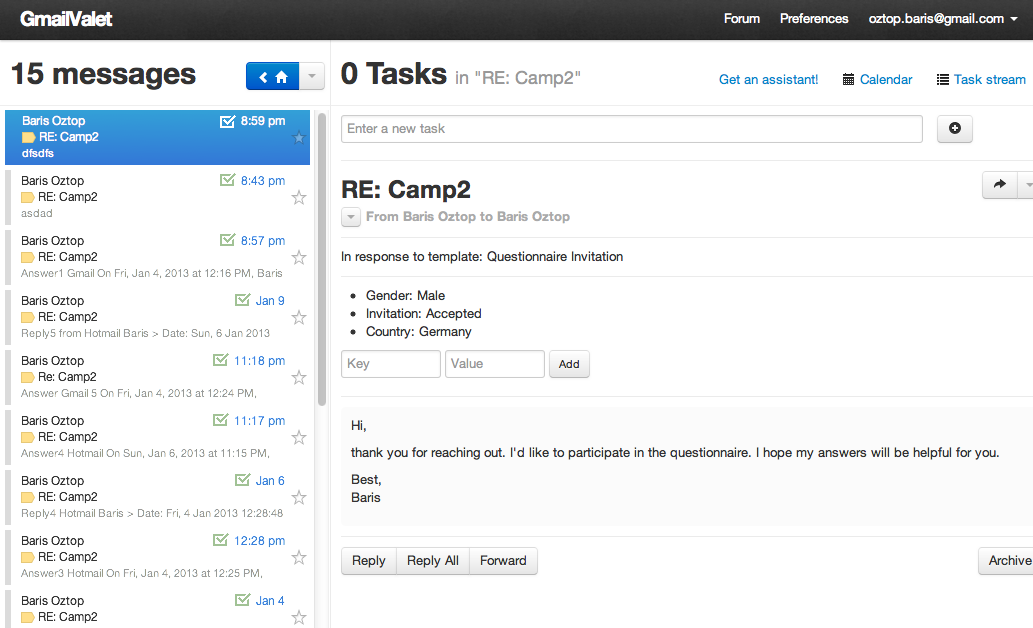
\includegraphics[width=1.00\textwidth]{imgs/GmailValetInbox.png}
	\caption[EmailValet Inbox View and Message Reading Pane]{EmailValet Inbox View and Message Reading Pane}
	\label{fig:GmailValetInbox}
\end{figure}

Starting a campaign is done exactly the same way as in composing an email. However, the corresponding view has two additional input fields to get the campaign's and the template's names from the user. A campaign name will help on identifying groups of conversations from other campaigns, or from regular email conversations in the inbox. A template name will help us identify which respondent's answers correspond to which emails that we sent. For example, in figure \ref{fig:GmailValetInbox}, a recipient's answer is the response to the questionnaire invitation that we sent earlier. A template name will also help us represent the template in a tree structure to pick from and reuse, and show the state of the conversation in the same tree structure.
\vspace{1cm}

The researchers can add their recipients list into the "Merge"\footnote{The word "merge" comes from the term "mail merge", which means a procedure to enable to combine a document with data files consisting a list of names. Therefore, the copies of the document will be different for each person it is sent to \citep{CollinsEnglishDictionary2013}.} input field as shown in figure \ref{fig:ComposePaneWithTemplates}, which corresponds to the "To" field in a regular email client. However, the format should be similar to the shown figure --- first name, last name, and email address written in angle brackets. Hence, those fields can be used dynamically in the salutation of the emails by writing one of the variables of \textit{\{\{first\_name\}\}} and \textit{\{\{last\_name\}\}}. Once the recipients list is entered, and the email is sent, these contacts will be recorded on Gmail's contacts book.
\vspace{1cm}

\begin{figure}[H]
	\centering
	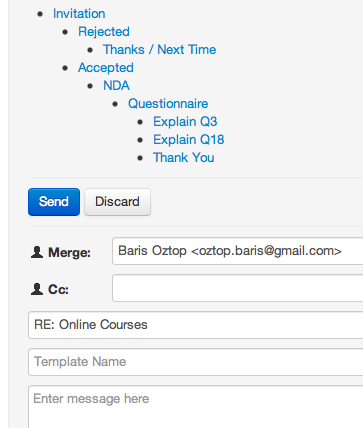
\includegraphics[scale=0.70]{imgs/ComposePaneWithTemplates.png}
	\caption[Email Template Selection to Reuse Earlier Replies]{Email Template Selection to Reuse Earlier Replies}
	\label{fig:ComposePaneWithTemplates}
\end{figure}

Figure \ref{fig:ComposePaneWithTemplates} also shows the template tree used to represent the state of the conversation, and allow users to select a template from. The indentation at the nodes of the tree helps on identifying which templates are used after which one and therefore it gives an idea about the current state and flow of the conversation. According to this sample scenario in the figure, right after we sent the invitation email and started on getting responses, there were two possible answers to give the recipients. For those who rejected the invitation, we can select the "Rejected" node from the tree to reuse an answer we gave before. This can be a motivation email as discussed in section \ref{subsec:4.1.2:ImprReduEffo}. On the same note, the people who accepted the invitation would receive a \ac{NDA}, and afterwards the questionnaire as the conversation with them carries on. After sending the questionnaire, there were cases where some respondents sent an email clarifying some questions found in the questionnaire. According to figure \ref{fig:ComposePaneWithTemplates}, these cases are related to the questions number 3 and 18, and we explained those questions, to clear off the confusion or issues they are having. Again, since the system allow us to reuse our previous answers as a template; we do not need to rewrite our explanation for those questions not clear for future queries. On the other hand, if the researchers wish to create a new template, he or she can simply do so by adding the name of the template into the corresponding input field, and send the email. The next time the researcher fires up the application, he or she will find it in the template tree under the corresponding level of the node. Also, it is possible to select a template, made some modifications on it and save it as a new template. Therefore, a slightly different version of the templates can be reused during the communication as well.
\vspace{1cm}

Finally, there is an option to add \ac{KVP}s while reading the respondents' answers. In the reading pane, two input fields are present, allowing users to enter a key and its value corresponding to the extracted information from those emails while reading them. As shown on figure \ref{fig:EMailKVPs}, as a user adds a new \ac{KVP}, they can also see the existing ones added earlier to that email message.
\vspace{1cm}

In the next section, we will address some implementation details about EmailValet's mass email communication modifications.

\begin{figure}[htbp]
	\centering
	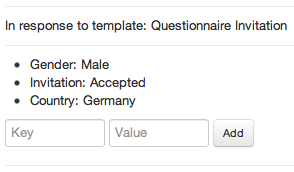
\includegraphics[scale=0.75]{imgs/EMailKVPs.png}
	\caption[Extracted Key-Value Pairs and Input Fields to Add New Ones]{Extracted Key-Value Pairs and Input Fields to Add New Ones}
	\label{fig:EMailKVPs}
\end{figure}

\subsection{Architecture}
\label{subsec:4.2.3:ProtArch}

Even though, we have a ready-to-use email client with EmailValet, there were quite many changes to reflect the requirements that were mentioned in section \ref{subsec:4.2.1:ProtReqiAnal}. Since EmailValet dealt with single email messages, and not a group of them as an email client, there were also some modifications needed to be done in order to make the prototype understand whether a message belongs to the campaign or not. In this section, we will briefly see how the changes for the prototype fit into the existing EmailValet's design, and make a technology overview to fully understand how a mass email communication is done.

\paragraph{Identification of a Campaign Message} \mbox{}\\
An email message consists of a header and body sections as defined by RFC 5322. While a message's header keeps structured information such as "From", "To", "\ac{CC}", Subject, Date, and other information with a special syntax, a message's body contains the content, which is an unstructured text and it is optional to have \citep{rfc5322}. An example email message with its header fields and body can be seen in Appendix \ref{app:EmaiMessForm}.
\vspace{1cm}

One of the fields in an email message's header is called Message-ID\footnote{The message identifier, Message-ID, is enclosed in the angle bracket characters, "<" and ">", an its syntax only permits the dot-atom-text form, which is \verb|1*atext *("." 1*atext)|, on the left-hand side of the "@" and a domain name is recommended for the right-hand side of the "@" \citep{rfc5322}. For example: \verb|<CAF2E4bfH4+GAYHcJFZJ6dTJJ+pux4mTjff2neCS_VR_zVCUY9g@mail.gmail.com>|}, which is a unique message identifier, and set by email clients. The value of a Message-ID is used in another header field, named "In-Reply-To", when a message is a reply to that message.
\vspace{1cm}

EmailValet had already the data model to store an email message's related data when it is synchronized\footnote{Fetching the emails from Gmail is done via the \ac{IMAP} extension that Gmail provides. \ac{IMAP} is a Internet message access standard defined by RFC3501. It allows a client to access and manipulate mail messages on server \citep{rfc3501}. On the other hand, EmailValet uses \ac{SMTP} protocol to connect to the Google's \ac{SMTP} servers to send a composed email in EmailValet. \ac{SMTP} is a mail transport and delivery protocol defined by RFC5321 \citep{rfc5321}.} with Gmail. However, creating a mass email campaign requires to identify if the synchronized email belongs to a mass email campaign created or if it is an answer to a campaign message that was sent before. Because EmailValet's initial design was able to fetch emails from Gmail, then assigning of different properties should follow. The emails composed by EmailValet comes to an existence in the EmailValet database after recipients send a reply to them, since EmailValet fetches them from Gmail's inbox as part of the thread of messages. Therefore, Message-ID and In-Reply-To fields of an email message are leveraged to keep track of a campaign message by setting a Message-ID into it, and store it in a "Campaign" data model as illustrated on \ref{fig:UML_Prototype}. With this, we were able to identify the type of messages during the synchronization with Gmail, whether the message is an initial campaign message, or if it is an answer to a campaign message that was created earlier. Before this, setting a Message-ID was done by EmailValet's "mail" gem\footnote{A Gem or a RubyGem is a software package, containing a packaged Ruby application or library \citep{RubyGemsGuides2013}.} during its execution time without allowing to get its value.

\clearpage

\begin{figure}[htbp]
	\centering
	\begin{pdfpic}
	    %LaTeX with PSTricks extensions
%%Creator: inkscape 0.48.2
%%Please note this file requires PSTricks extensions
\psset{xunit=.5pt,yunit=.5pt,runit=.5pt}
\begin{pspicture}(877.5,587.5)
{
\newrgbcolor{curcolor}{1 1 1}
\pscustom[linestyle=none,fillstyle=solid,fillcolor=curcolor]
{
\newpath
\moveto(0,517.00488125)
\lineto(772.2,517.00488125)
\lineto(772.2,0.00488125)
\lineto(0,0.00488125)
\closepath
}
}
{
\newrgbcolor{curcolor}{1 1 1}
\pscustom[linestyle=none,fillstyle=solid,fillcolor=curcolor]
{
\newpath
\moveto(1.1,468.60488125)
\lineto(240.788284,468.60488125)
\lineto(240.788284,376.20488125)
\lineto(1.1,376.20488125)
\closepath
\moveto(1.1,468.60488125)
}
}
{
\newrgbcolor{curcolor}{0 0 0}
\pscustom[linewidth=2.20000003,linecolor=curcolor]
{
\newpath
\moveto(1.1,468.60488125)
\lineto(240.788284,468.60488125)
\lineto(240.788284,376.20488125)
\lineto(1.1,376.20488125)
\closepath
\moveto(1.1,468.60488125)
}
}
{
\newrgbcolor{curcolor}{0 0 0}
\pscustom[linestyle=none,fillstyle=solid,fillcolor=curcolor]
{
\newpath
\moveto(79.13984375,460.54394375)
\lineto(83.35078125,460.54394375)
\lineto(86.27265625,453.66894375)
\lineto(89.21171875,460.54394375)
\lineto(93.42265625,460.54394375)
\lineto(93.42265625,447.70488125)
\lineto(90.29453125,447.70488125)
\lineto(90.29453125,457.08925625)
\lineto(87.33828125,450.17988125)
\lineto(85.24140625,450.17988125)
\lineto(82.28515625,457.08925625)
\lineto(82.28515625,447.70488125)
\lineto(79.13984375,447.70488125)
\closepath
\moveto(79.13984375,460.54394375)
}
}
{
\newrgbcolor{curcolor}{0 0 0}
\pscustom[linestyle=none,fillstyle=solid,fillcolor=curcolor]
{
\newpath
\moveto(106.11992188,452.55175625)
\lineto(106.11992188,451.67519375)
\lineto(98.93554688,451.67519375)
\curveto(99.00429688,450.95331875)(99.26210938,450.40761535)(99.70898438,450.04238125)
\curveto(100.15585938,449.68574035)(100.77890598,449.50956875)(101.58242188,449.50956875)
\curveto(102.23554687,449.50956875)(102.89726617,449.59980285)(103.57617188,449.78456875)
\curveto(104.25078097,449.97792785)(104.95117188,450.27011535)(105.67304688,450.66113125)
\lineto(105.67304688,448.28925625)
\curveto(104.93828097,448.01425625)(104.20351618,447.80800625)(103.47304688,447.67050625)
\curveto(102.75117187,447.52441305)(102.02929688,447.44706875)(101.30742188,447.44706875)
\curveto(99.56289118,447.44706875)(98.20507758,447.88534945)(97.23398438,448.77050625)
\curveto(96.27148438,449.66425625)(95.79023437,450.91034945)(95.79023437,452.51738125)
\curveto(95.79023437,454.08574035)(96.26289118,455.31894375)(97.21679688,456.21269375)
\curveto(98.16640598,457.11503805)(99.47265598,457.57050625)(101.13554688,457.57050625)
\curveto(102.64804688,457.57050625)(103.85546848,457.11074035)(104.76210938,456.19550625)
\curveto(105.66445257,455.28886535)(106.11992188,454.07284945)(106.11992188,452.55175625)
\closepath
\moveto(102.95742188,453.56581875)
\curveto(102.95742188,454.15019375)(102.78554688,454.61855285)(102.44179688,454.97519375)
\curveto(102.10664118,455.34042785)(101.66835938,455.52519375)(101.11835937,455.52519375)
\curveto(100.52109348,455.52519375)(100.03554688,455.35331875)(99.65742187,455.00956875)
\curveto(99.28789117,454.67441305)(99.06015598,454.19316305)(98.96992187,453.56581875)
\closepath
\moveto(102.95742188,453.56581875)
}
}
{
\newrgbcolor{curcolor}{0 0 0}
\pscustom[linestyle=none,fillstyle=solid,fillcolor=curcolor]
{
\newpath
\moveto(115.98554688,457.03769375)
\lineto(115.98554688,454.70019375)
\curveto(115.31953098,454.97519375)(114.67929688,455.18144375)(114.06054688,455.31894375)
\curveto(113.45039008,455.45644375)(112.87890598,455.52519375)(112.34179688,455.52519375)
\curveto(111.75742188,455.52519375)(111.31914008,455.44784945)(111.03554688,455.30175625)
\curveto(110.74765598,455.15136535)(110.60585938,454.92792785)(110.60585938,454.63144375)
\curveto(110.60585938,454.37792785)(110.71328098,454.18456875)(110.93242188,454.04706875)
\curveto(111.14726508,453.91816305)(111.53398438,453.82792785)(112.08398438,453.77206875)
\lineto(112.63398437,453.68613125)
\curveto(114.20234348,453.48847445)(115.25507868,453.16191305)(115.79648438,452.70644375)
\curveto(116.34648438,452.24667785)(116.62148438,451.52480285)(116.62148438,450.54081875)
\curveto(116.62148438,449.51816305)(116.24335938,448.74472445)(115.48710938,448.22050625)
\curveto(114.73085938,447.70488125)(113.60078098,447.44706875)(112.10117188,447.44706875)
\curveto(111.46953097,447.44706875)(110.81210938,447.49863125)(110.12460938,447.60175625)
\curveto(109.44570368,447.70488125)(108.75390598,447.85956875)(108.04492188,448.06581875)
\lineto(108.04492188,450.40331875)
\curveto(108.65078098,450.10253805)(109.27382868,449.87909945)(109.91835938,449.73300625)
\curveto(110.57148437,449.58261535)(111.22890598,449.50956875)(111.89492188,449.50956875)
\curveto(112.48789008,449.50956875)(112.93476508,449.58691305)(113.23554687,449.75019375)
\curveto(113.54492188,449.92206875)(113.69960938,450.16699035)(113.69960938,450.48925625)
\curveto(113.69960938,450.76425625)(113.59648438,450.97050625)(113.39023438,451.10800625)
\curveto(113.18398438,451.24550625)(112.76289008,451.34863125)(112.13554688,451.41738125)
\lineto(111.60273437,451.48613125)
\curveto(110.22773437,451.65800625)(109.26523438,451.97167785)(108.71523438,452.43144375)
\curveto(108.16523437,452.89980285)(107.89023438,453.60878805)(107.89023438,454.56269375)
\curveto(107.89023438,455.58105285)(108.23828098,456.33730285)(108.93867187,456.83144375)
\curveto(109.63476508,457.32128805)(110.70898438,457.57050625)(112.15273438,457.57050625)
\curveto(112.72421848,457.57050625)(113.32148437,457.52324035)(113.94023438,457.43300625)
\curveto(114.56757868,457.35136535)(115.25078097,457.21816305)(115.98554688,457.03769375)
\closepath
\moveto(115.98554688,457.03769375)
}
}
{
\newrgbcolor{curcolor}{0 0 0}
\pscustom[linestyle=none,fillstyle=solid,fillcolor=curcolor]
{
\newpath
\moveto(126.46992188,457.03769375)
\lineto(126.46992188,454.70019375)
\curveto(125.80390598,454.97519375)(125.16367188,455.18144375)(124.54492188,455.31894375)
\curveto(123.93476508,455.45644375)(123.36328098,455.52519375)(122.82617188,455.52519375)
\curveto(122.24179688,455.52519375)(121.80351508,455.44784945)(121.51992188,455.30175625)
\curveto(121.23203098,455.15136535)(121.09023438,454.92792785)(121.09023438,454.63144375)
\curveto(121.09023438,454.37792785)(121.19765598,454.18456875)(121.41679688,454.04706875)
\curveto(121.63164008,453.91816305)(122.01835938,453.82792785)(122.56835938,453.77206875)
\lineto(123.11835937,453.68613125)
\curveto(124.68671848,453.48847445)(125.73945368,453.16191305)(126.28085938,452.70644375)
\curveto(126.83085938,452.24667785)(127.10585938,451.52480285)(127.10585938,450.54081875)
\curveto(127.10585938,449.51816305)(126.72773438,448.74472445)(125.97148438,448.22050625)
\curveto(125.21523438,447.70488125)(124.08515598,447.44706875)(122.58554688,447.44706875)
\curveto(121.95390597,447.44706875)(121.29648438,447.49863125)(120.60898438,447.60175625)
\curveto(119.93007868,447.70488125)(119.23828098,447.85956875)(118.52929688,448.06581875)
\lineto(118.52929688,450.40331875)
\curveto(119.13515598,450.10253805)(119.75820368,449.87909945)(120.40273438,449.73300625)
\curveto(121.05585937,449.58261535)(121.71328098,449.50956875)(122.37929688,449.50956875)
\curveto(122.97226508,449.50956875)(123.41914008,449.58691305)(123.71992187,449.75019375)
\curveto(124.02929688,449.92206875)(124.18398438,450.16699035)(124.18398438,450.48925625)
\curveto(124.18398438,450.76425625)(124.08085938,450.97050625)(123.87460938,451.10800625)
\curveto(123.66835938,451.24550625)(123.24726508,451.34863125)(122.61992188,451.41738125)
\lineto(122.08710937,451.48613125)
\curveto(120.71210937,451.65800625)(119.74960938,451.97167785)(119.19960938,452.43144375)
\curveto(118.64960937,452.89980285)(118.37460938,453.60878805)(118.37460938,454.56269375)
\curveto(118.37460938,455.58105285)(118.72265598,456.33730285)(119.42304687,456.83144375)
\curveto(120.11914008,457.32128805)(121.19335938,457.57050625)(122.63710938,457.57050625)
\curveto(123.20859348,457.57050625)(123.80585937,457.52324035)(124.42460938,457.43300625)
\curveto(125.05195368,457.35136535)(125.73515597,457.21816305)(126.46992188,457.03769375)
\closepath
\moveto(126.46992188,457.03769375)
}
}
{
\newrgbcolor{curcolor}{0 0 0}
\pscustom[linestyle=none,fillstyle=solid,fillcolor=curcolor]
{
\newpath
\moveto(133.74023438,452.03613125)
\curveto(133.09570368,452.03613125)(132.61445368,451.92441305)(132.29648438,451.70956875)
\curveto(131.97421848,451.49042785)(131.81523438,451.16816305)(131.81523438,450.74706875)
\curveto(131.81523438,450.35605285)(131.93984348,450.05097445)(132.19335938,449.83613125)
\curveto(132.45546848,449.61699035)(132.82070368,449.50956875)(133.29335938,449.50956875)
\curveto(133.86484348,449.50956875)(134.34609348,449.71581875)(134.73710938,450.12831875)
\curveto(135.13671848,450.54081875)(135.33867188,451.06074035)(135.33867188,451.69238125)
\lineto(135.33867188,452.03613125)
\closepath
\moveto(138.44960938,453.20488125)
\lineto(138.44960938,447.70488125)
\lineto(135.33867188,447.70488125)
\lineto(135.33867188,449.13144375)
\curveto(134.92617188,448.54706875)(134.46210938,448.11738125)(133.94648438,447.84238125)
\curveto(133.43085938,447.58027215)(132.80351508,447.44706875)(132.07304688,447.44706875)
\curveto(131.07617188,447.44706875)(130.25976508,447.73925625)(129.63242188,448.32363125)
\curveto(129.01367188,448.90800625)(128.70429688,449.66425625)(128.70429688,450.59238125)
\curveto(128.70429688,451.72675625)(129.09101508,452.55605285)(129.87304688,453.08456875)
\curveto(130.65078098,453.60878805)(131.87109348,453.87519375)(133.53398438,453.87519375)
\lineto(135.33867188,453.87519375)
\lineto(135.33867188,454.11581875)
\curveto(135.33867188,454.59706875)(135.14101508,454.94941305)(134.75429688,455.18144375)
\curveto(134.37617188,455.40917785)(133.77890598,455.52519375)(132.96679688,455.52519375)
\curveto(132.31367188,455.52519375)(131.69921848,455.45644375)(131.12773438,455.31894375)
\curveto(130.56484348,455.19003805)(130.03632868,454.99667785)(129.54648438,454.73456875)
\lineto(129.54648438,457.07206875)
\curveto(130.20820368,457.23105285)(130.87421848,457.35136535)(131.54023438,457.43300625)
\curveto(132.20195368,457.52324035)(132.86796848,457.57050625)(133.53398438,457.57050625)
\curveto(135.26132868,457.57050625)(136.51171848,457.22675625)(137.28085938,456.53925625)
\curveto(138.05859348,455.85175625)(138.44960938,454.73886535)(138.44960938,453.20488125)
\closepath
\moveto(138.44960938,453.20488125)
}
}
{
\newrgbcolor{curcolor}{0 0 0}
\pscustom[linestyle=none,fillstyle=solid,fillcolor=curcolor]
{
\newpath
\moveto(147.85546875,449.33769375)
\curveto(147.43007785,448.77480285)(146.96171875,448.36230285)(146.44609375,448.10019375)
\curveto(145.93906305,447.83378805)(145.35468805,447.70488125)(144.69296875,447.70488125)
\curveto(143.51132785,447.70488125)(142.53593805,448.16894375)(141.77109375,449.09706875)
\curveto(141.00195285,450.02519375)(140.61953125,451.20253805)(140.61953125,452.63769375)
\curveto(140.61953125,454.06855285)(141.00195285,455.24159945)(141.77109375,456.16113125)
\curveto(142.53593805,457.08925625)(143.51132785,457.55331875)(144.69296875,457.55331875)
\curveto(145.35468805,457.55331875)(145.93906305,457.42011535)(146.44609375,457.15800625)
\curveto(146.96171875,456.89159945)(147.43007785,456.47480285)(147.85546875,455.90331875)
\lineto(147.85546875,457.32988125)
\lineto(150.94921875,457.32988125)
\lineto(150.94921875,448.68456875)
\curveto(150.94921875,447.12909945)(150.45937445,445.94316305)(149.48828125,445.12675625)
\curveto(148.51289035,444.31464715)(147.09921875,443.90644375)(145.24296875,443.90644375)
\curveto(144.63281305,443.90644375)(144.04843805,443.95370965)(143.48984375,444.04394375)
\curveto(142.92695285,444.13847445)(142.36406305,444.27597445)(141.80546875,444.45644375)
\lineto(141.80546875,446.86269375)
\curveto(142.34257785,446.55331875)(142.87109375,446.32558465)(143.38671875,446.17519375)
\curveto(143.90234375,446.01620965)(144.41796875,445.93456875)(144.93359375,445.93456875)
\curveto(145.93906305,445.93456875)(146.67812445,446.15800625)(147.15078125,446.60488125)
\curveto(147.61914035,447.04316305)(147.85546875,447.7306625)(147.85546875,448.68456875)
\closepath
\moveto(145.82734375,455.33613125)
\curveto(145.19570285,455.33613125)(144.70156305,455.09980285)(144.34921875,454.63144375)
\curveto(143.99257785,454.15878805)(143.81640625,453.49706875)(143.81640625,452.63769375)
\curveto(143.81640625,451.75253805)(143.98828125,451.08222445)(144.33203125,450.62675625)
\curveto(144.67578125,450.16699035)(145.17421875,449.93925625)(145.82734375,449.93925625)
\curveto(146.46757785,449.93925625)(146.96601535,450.17128805)(147.32265625,450.64394375)
\curveto(147.67499945,451.11230285)(147.85546875,451.77831875)(147.85546875,452.63769375)
\curveto(147.85546875,453.49706875)(147.67499945,454.15878805)(147.32265625,454.63144375)
\curveto(146.96601535,455.09980285)(146.46757785,455.33613125)(145.82734375,455.33613125)
\closepath
\moveto(145.82734375,455.33613125)
}
}
{
\newrgbcolor{curcolor}{0 0 0}
\pscustom[linestyle=none,fillstyle=solid,fillcolor=curcolor]
{
\newpath
\moveto(163.5046875,452.55175625)
\lineto(163.5046875,451.67519375)
\lineto(156.3203125,451.67519375)
\curveto(156.3890625,450.95331875)(156.646875,450.40761535)(157.09375,450.04238125)
\curveto(157.540625,449.68574035)(158.1636716,449.50956875)(158.9671875,449.50956875)
\curveto(159.6203125,449.50956875)(160.2820318,449.59980285)(160.9609375,449.78456875)
\curveto(161.6355466,449.97792785)(162.3359375,450.27011535)(163.0578125,450.66113125)
\lineto(163.0578125,448.28925625)
\curveto(162.3230466,448.01425625)(161.5882818,447.80800625)(160.8578125,447.67050625)
\curveto(160.1359375,447.52441305)(159.4140625,447.44706875)(158.6921875,447.44706875)
\curveto(156.9476568,447.44706875)(155.5898432,447.88534945)(154.61875,448.77050625)
\curveto(153.65625,449.66425625)(153.175,450.91034945)(153.175,452.51738125)
\curveto(153.175,454.08574035)(153.6476568,455.31894375)(154.6015625,456.21269375)
\curveto(155.5511716,457.11503805)(156.8574216,457.57050625)(158.5203125,457.57050625)
\curveto(160.0328125,457.57050625)(161.2402341,457.11074035)(162.146875,456.19550625)
\curveto(163.0492182,455.28886535)(163.5046875,454.07284945)(163.5046875,452.55175625)
\closepath
\moveto(160.3421875,453.56581875)
\curveto(160.3421875,454.15019375)(160.1703125,454.61855285)(159.8265625,454.97519375)
\curveto(159.4914068,455.34042785)(159.053125,455.52519375)(158.503125,455.52519375)
\curveto(157.9058591,455.52519375)(157.4203125,455.35331875)(157.0421875,455.00956875)
\curveto(156.6726568,454.67441305)(156.4449216,454.19316305)(156.3546875,453.56581875)
\closepath
\moveto(160.3421875,453.56581875)
}
}
{
\newrgbcolor{curcolor}{0 0 0}
\pscustom[linestyle=none,fillstyle=solid,fillcolor=curcolor]
{
\newpath
\moveto(18.4679698,439.47206875)
\lineto(24.0367198,439.47206875)
\lineto(23.8476573,438.47519375)
\lineto(19.4648448,438.47519375)
\lineto(18.9492198,435.86269375)
\lineto(23.1601573,435.86269375)
\lineto(22.9710948,434.84863125)
\lineto(18.7601573,434.84863125)
\lineto(18.1414073,431.65175625)
\lineto(22.6273448,431.65175625)
\lineto(22.4382823,430.65488125)
\lineto(16.7492198,430.65488125)
\closepath
\moveto(18.4679698,439.47206875)
}
}
{
\newrgbcolor{curcolor}{0 0 0}
\pscustom[linestyle=none,fillstyle=solid,fillcolor=curcolor]
{
\newpath
\moveto(31.32421875,437.27206875)
\lineto(28.29921875,434.02363125)
\lineto(30.15546875,430.65488125)
\lineto(28.91796875,430.65488125)
\lineto(27.50859375,433.28456875)
\lineto(25.06796875,430.65488125)
\lineto(23.76171875,430.65488125)
\lineto(27.01015625,434.14394375)
\lineto(25.27421875,437.27206875)
\lineto(26.52890625,437.27206875)
\lineto(27.80078125,434.88300625)
\lineto(30.01796875,437.27206875)
\closepath
\moveto(31.32421875,437.27206875)
}
}
{
\newrgbcolor{curcolor}{0 0 0}
\pscustom[linestyle=none,fillstyle=solid,fillcolor=curcolor]
{
\newpath
\moveto(33.44257813,439.85019375)
\lineto(34.52539062,439.85019375)
\lineto(34.26757812,438.47519375)
\lineto(33.16757813,438.47519375)
\closepath
\moveto(32.94414063,437.27206875)
\lineto(34.02695313,437.27206875)
\lineto(32.73789063,430.65488125)
\lineto(31.65507813,430.65488125)
\closepath
\moveto(32.94414063,437.27206875)
}
}
{
\newrgbcolor{curcolor}{0 0 0}
\pscustom[linestyle=none,fillstyle=solid,fillcolor=curcolor]
{
\newpath
\moveto(40.62695312,437.08300625)
\lineto(40.42070313,436.05175625)
\curveto(40.13281223,436.21074035)(39.82773493,436.32675625)(39.50976562,436.39550625)
\curveto(39.18749973,436.47284945)(38.86093723,436.51581875)(38.53007813,436.51581875)
\curveto(37.95429633,436.51581875)(37.50312473,436.41699035)(37.17226563,436.22363125)
\curveto(36.83710993,436.02597445)(36.67382812,435.76386535)(36.67382812,435.43300625)
\curveto(36.67382812,435.04199035)(37.05624973,434.74550625)(37.82539063,434.53925625)
\curveto(37.88124973,434.51347445)(37.92851563,434.50488125)(37.96289062,434.50488125)
\lineto(38.30664062,434.40175625)
\curveto(39.02851563,434.19550625)(39.50976562,433.98066305)(39.75039063,433.76581875)
\curveto(39.99101563,433.54667785)(40.11132812,433.24159945)(40.11132812,432.85488125)
\curveto(40.11132812,432.15449035)(39.82773493,431.58300625)(39.26914063,431.13613125)
\curveto(38.71914063,430.69785)(37.98867133,430.48300625)(37.08632813,430.48300625)
\curveto(36.74257813,430.48300625)(36.37304633,430.51738125)(35.98632812,430.58613125)
\curveto(35.59531223,430.65488125)(35.16992133,430.75800625)(34.71445313,430.89550625)
\lineto(34.92070313,432.01269375)
\curveto(35.32031223,431.81503805)(35.71132813,431.66034945)(36.08945313,431.54863125)
\curveto(36.47617133,431.44550625)(36.84999973,431.39394375)(37.20664063,431.39394375)
\curveto(37.74374973,431.39394375)(38.17773493,431.50566305)(38.51289063,431.73769375)
\curveto(38.84374973,431.96542785)(39.01132813,432.25331875)(39.01132813,432.59706875)
\curveto(39.01132813,432.97519375)(38.57304632,433.28456875)(37.70507812,433.52519375)
\lineto(37.58476563,433.54238125)
\lineto(37.20664063,433.64550625)
\curveto(36.65664063,433.79159945)(36.25273493,433.98066305)(36.00351563,434.21269375)
\curveto(35.74999973,434.45331875)(35.62539063,434.76269375)(35.62539063,435.14081875)
\curveto(35.62539063,435.83691305)(35.88749973,436.39550625)(36.41601562,436.80800625)
\curveto(36.94023493,437.22050625)(37.65781223,437.42675625)(38.56445312,437.42675625)
\curveto(38.92968723,437.42675625)(39.27773493,437.39667785)(39.61289063,437.34081875)
\curveto(39.95664063,437.28066305)(40.29179633,437.19472445)(40.62695312,437.08300625)
\closepath
\moveto(40.62695312,437.08300625)
}
}
{
\newrgbcolor{curcolor}{0 0 0}
\pscustom[linestyle=none,fillstyle=solid,fillcolor=curcolor]
{
\newpath
\moveto(45.99375,437.27206875)
\lineto(45.821875,436.42988125)
\lineto(43.65625,436.42988125)
\lineto(42.9515625,432.83769375)
\curveto(42.9257818,432.70019375)(42.9085932,432.58417785)(42.9,432.49394375)
\curveto(42.8871091,432.39941305)(42.8828125,432.33066305)(42.8828125,432.28769375)
\curveto(42.8828125,432.03417785)(42.9558591,431.84941305)(43.10625,431.73769375)
\curveto(43.2523432,431.62167785)(43.5015625,431.56581875)(43.8453125,431.56581875)
\lineto(44.9453125,431.56581875)
\lineto(44.75625,430.65488125)
\lineto(43.7078125,430.65488125)
\curveto(43.0632818,430.65488125)(42.5820318,430.77949035)(42.2640625,431.03300625)
\curveto(41.9546875,431.28222445)(41.8,431.66894375)(41.8,432.18456875)
\curveto(41.8,432.27480285)(41.8042966,432.37363125)(41.8171875,432.47675625)
\curveto(41.8257818,432.58847445)(41.8429682,432.70878805)(41.86875,432.83769375)
\lineto(42.5734375,436.42988125)
\lineto(41.6453125,436.42988125)
\lineto(41.8171875,437.27206875)
\lineto(42.728125,437.27206875)
\lineto(43.0890625,439.14550625)
\lineto(44.171875,439.14550625)
\lineto(43.8109375,437.27206875)
\closepath
\moveto(45.99375,437.27206875)
}
}
{
\newrgbcolor{curcolor}{0 0 0}
\pscustom[linestyle=none,fillstyle=solid,fillcolor=curcolor]
{
\newpath
\moveto(47.83710938,439.85019375)
\lineto(48.91992188,439.85019375)
\lineto(48.66210938,438.47519375)
\lineto(47.56210938,438.47519375)
\closepath
\moveto(47.33867188,437.27206875)
\lineto(48.42148438,437.27206875)
\lineto(47.13242188,430.65488125)
\lineto(46.04960938,430.65488125)
\closepath
\moveto(47.33867188,437.27206875)
}
}
{
\newrgbcolor{curcolor}{0 0 0}
\pscustom[linestyle=none,fillstyle=solid,fillcolor=curcolor]
{
\newpath
\moveto(55.70898438,434.64238125)
\lineto(54.93554688,430.65488125)
\lineto(53.85273438,430.65488125)
\lineto(54.62617188,434.60800625)
\curveto(54.66054688,434.78847445)(54.68203098,434.95175625)(54.69492188,435.08925625)
\curveto(54.71640598,435.23534945)(54.72929688,435.35136535)(54.72929688,435.43300625)
\curveto(54.72929688,435.76386535)(54.62617188,436.02167785)(54.41992188,436.20644375)
\curveto(54.21367188,436.38691305)(53.92148438,436.48144375)(53.54335938,436.48144375)
\curveto(52.95898438,436.48144375)(52.45195257,436.28378805)(52.03085938,435.89706875)
\curveto(51.61835938,435.51894375)(51.34335938,434.99042785)(51.20585938,434.31581875)
\lineto(50.48398438,430.65488125)
\lineto(49.40117188,430.65488125)
\lineto(50.67304688,437.27206875)
\lineto(51.77304688,437.27206875)
\lineto(51.54960938,436.24081875)
\curveto(51.84609348,436.61894375)(52.20703098,436.91113125)(52.63242188,437.11738125)
\curveto(53.06640598,437.32363125)(53.51757758,437.42675625)(53.99023438,437.42675625)
\curveto(54.56171848,437.42675625)(55.00859348,437.26347445)(55.33085938,436.94550625)
\curveto(55.64882758,436.63613125)(55.81210938,436.19355285)(55.81210938,435.62206875)
\curveto(55.81210938,435.48456875)(55.79921848,435.33417785)(55.77773438,435.17519375)
\curveto(55.76484348,435.01191305)(55.74335938,434.83574035)(55.70898438,434.64238125)
\closepath
\moveto(55.70898438,434.64238125)
}
}
{
\newrgbcolor{curcolor}{0 0 0}
\pscustom[linestyle=none,fillstyle=solid,fillcolor=curcolor]
{
\newpath
\moveto(63.86015625,437.27206875)
\lineto(62.72578125,431.47988125)
\curveto(62.50664035,430.35839715)(62.08984375,429.52050625)(61.47109375,428.97050625)
\curveto(60.86093805,428.42050625)(60.04453125,428.14550625)(59.01328125,428.14550625)
\curveto(58.63515625,428.14550625)(58.27851535,428.17558465)(57.94765625,428.23144375)
\curveto(57.61249945,428.29159945)(57.31171875,428.37753805)(57.03671875,428.48925625)
\lineto(57.22578125,429.53769375)
\curveto(57.50078125,429.36581875)(57.78437445,429.24120965)(58.08515625,429.15956875)
\curveto(58.38164035,429.08222445)(58.70390625,429.03925625)(59.04765625,429.03925625)
\curveto(59.73515625,429.03925625)(60.29374945,429.22831875)(60.73203125,429.60644375)
\curveto(61.17890625,429.97597445)(61.47109375,430.51308465)(61.60859375,431.22206875)
\lineto(61.71171875,431.72050625)
\curveto(61.40234375,431.37675625)(61.04570285,431.11034945)(60.64609375,430.92988125)
\curveto(60.24218805,430.74511557)(59.81249945,430.65488125)(59.35703125,430.65488125)
\curveto(58.67812445,430.65488125)(58.14531305,430.86972445)(57.75859375,431.30800625)
\curveto(57.38046875,431.75488125)(57.19140625,432.36503805)(57.19140625,433.14706875)
\curveto(57.19140625,433.75292785)(57.30312445,434.35019375)(57.53515625,434.93456875)
\curveto(57.77578125,435.51894375)(58.10664035,436.03886535)(58.53203125,436.49863125)
\curveto(58.80703125,436.79511535)(59.12499945,437.02284945)(59.49453125,437.18613125)
\curveto(59.87265625,437.34511535)(60.25937445,437.42675625)(60.66328125,437.42675625)
\curveto(61.11015625,437.42675625)(61.49687445,437.32363125)(61.83203125,437.11738125)
\curveto(62.16289035,436.91113125)(62.40781305,436.61894375)(62.57109375,436.24081875)
\lineto(62.76015625,437.27206875)
\closepath
\moveto(62.22734375,434.84863125)
\curveto(62.22734375,435.37284945)(62.09843805,435.78105285)(61.84921875,436.06894375)
\curveto(61.59570285,436.36542785)(61.23476535,436.51581875)(60.76640625,436.51581875)
\curveto(60.47851535,436.51581875)(60.20351535,436.45566305)(59.94140625,436.34394375)
\curveto(59.67499945,436.22792785)(59.45156305,436.07324035)(59.27109375,435.87988125)
\curveto(58.97031305,435.53613125)(58.73828125,435.13222445)(58.56640625,434.67675625)
\curveto(58.40312445,434.21699035)(58.32578125,433.74003805)(58.32578125,433.25019375)
\curveto(58.32578125,432.70878805)(58.45039035,432.29199035)(58.70390625,431.99550625)
\curveto(58.95312445,431.70761535)(59.32265625,431.56581875)(59.80390625,431.56581875)
\curveto(60.49140625,431.56581875)(61.06289035,431.87519375)(61.52265625,432.49394375)
\curveto(61.99101535,433.12128805)(62.22734375,433.90761535)(62.22734375,434.84863125)
\closepath
\moveto(62.22734375,434.84863125)
}
}
{
\newrgbcolor{curcolor}{0 0 0}
\pscustom[linestyle=none,fillstyle=solid,fillcolor=curcolor]
{
\newpath
\moveto(70.22382812,439.47206875)
\lineto(75.79257813,439.47206875)
\lineto(75.60351562,438.47519375)
\lineto(71.22070312,438.47519375)
\lineto(70.70507812,435.86269375)
\lineto(74.91601562,435.86269375)
\lineto(74.72695313,434.84863125)
\lineto(70.51601563,434.84863125)
\lineto(69.89726563,431.65175625)
\lineto(74.38320313,431.65175625)
\lineto(74.19414063,430.65488125)
\lineto(68.50507812,430.65488125)
\closepath
\moveto(70.22382812,439.47206875)
}
}
{
\newrgbcolor{curcolor}{0 0 0}
\pscustom[linestyle=none,fillstyle=solid,fillcolor=curcolor]
{
\newpath
\moveto(86.68945312,434.64238125)
\lineto(85.91601562,430.65488125)
\lineto(84.83320313,430.65488125)
\lineto(85.58945313,434.60800625)
\curveto(85.62382813,434.77988125)(85.64531222,434.92167785)(85.65820312,435.03769375)
\curveto(85.67968723,435.16230285)(85.69257813,435.26972445)(85.69257813,435.36425625)
\curveto(85.69257813,435.71659945)(85.58945313,435.99159945)(85.38320313,436.18925625)
\curveto(85.18554633,436.38261535)(84.91054632,436.48144375)(84.55820313,436.48144375)
\curveto(84.02968723,436.48144375)(83.56132813,436.27949035)(83.14882813,435.87988125)
\curveto(82.73632812,435.48886535)(82.46992133,434.97753805)(82.35820313,434.35019375)
\lineto(81.61914062,430.65488125)
\lineto(80.53632812,430.65488125)
\lineto(81.30976562,434.60800625)
\curveto(81.34414063,434.75409945)(81.36562473,434.89159945)(81.37851563,435.02050625)
\curveto(81.39999973,435.14511535)(81.41289063,435.25253805)(81.41289063,435.34706875)
\curveto(81.41289063,435.71230285)(81.30976562,435.99159945)(81.10351562,436.18925625)
\curveto(80.90585993,436.38261535)(80.63945313,436.48144375)(80.29570313,436.48144375)
\curveto(79.75429632,436.48144375)(79.28164063,436.27949035)(78.86914062,435.87988125)
\curveto(78.45664063,435.48886535)(78.18593723,434.97753805)(78.06132813,434.35019375)
\lineto(77.33945313,430.65488125)
\lineto(76.25664063,430.65488125)
\lineto(77.54570313,437.27206875)
\lineto(78.62851563,437.27206875)
\lineto(78.42226563,436.24081875)
\curveto(78.71874973,436.62753805)(79.06249973,436.91972445)(79.45351563,437.11738125)
\curveto(79.85312473,437.32363125)(80.28281223,437.42675625)(80.74257813,437.42675625)
\curveto(81.22382812,437.42675625)(81.61914062,437.29784945)(81.92851563,437.04863125)
\curveto(82.23789063,436.79511535)(82.41835993,436.44706875)(82.47851562,436.00019375)
\curveto(82.80937472,436.46855285)(83.19179632,436.82519375)(83.63007812,437.06581875)
\curveto(84.06406223,437.30644375)(84.52382813,437.42675625)(85.00507813,437.42675625)
\curveto(85.57656223,437.42675625)(86.01914063,437.25917785)(86.32851563,436.92831875)
\curveto(86.63789063,436.60605285)(86.79257813,436.14628805)(86.79257813,435.55331875)
\curveto(86.79257813,435.42441305)(86.77968723,435.28261535)(86.75820313,435.12363125)
\curveto(86.74531223,434.96034945)(86.72382813,434.80136535)(86.68945312,434.64238125)
\closepath
\moveto(86.68945312,434.64238125)
}
}
{
\newrgbcolor{curcolor}{0 0 0}
\pscustom[linestyle=none,fillstyle=solid,fillcolor=curcolor]
{
\newpath
\moveto(94.11875,434.43613125)
\lineto(93.3796875,430.65488125)
\lineto(92.296875,430.65488125)
\lineto(92.503125,431.65175625)
\curveto(92.1808591,431.26074035)(91.815625,430.96855285)(91.403125,430.77519375)
\curveto(90.9992182,430.58183443)(90.5480466,430.48300625)(90.0453125,430.48300625)
\curveto(89.4824216,430.48300625)(89.0183591,430.65488125)(88.653125,430.99863125)
\curveto(88.2964841,431.34238125)(88.1203125,431.78066305)(88.1203125,432.32206875)
\curveto(88.1203125,433.09980285)(88.4210932,433.71425625)(89.03125,434.16113125)
\curveto(89.65,434.60800625)(90.5007818,434.83144375)(91.5921875,434.83144375)
\lineto(93.1046875,434.83144375)
\lineto(93.15625,435.12363125)
\curveto(93.1648432,435.15800625)(93.1734375,435.19238125)(93.1734375,435.22675625)
\curveto(93.1820318,435.26113125)(93.190625,435.31699035)(93.190625,435.39863125)
\curveto(93.190625,435.75097445)(93.0445318,436.02597445)(92.7609375,436.22363125)
\curveto(92.4730466,436.41699035)(92.0734375,436.51581875)(91.5578125,436.51581875)
\curveto(91.2011716,436.51581875)(90.8359375,436.46855285)(90.4578125,436.37831875)
\curveto(90.0882818,436.28378805)(89.7101568,436.14628805)(89.3234375,435.96581875)
\lineto(89.5125,436.96269375)
\curveto(89.9121091,437.12167785)(90.3074216,437.23769375)(90.6984375,437.30644375)
\curveto(91.0980466,437.38378805)(91.4804682,437.42675625)(91.85,437.42675625)
\curveto(92.6277341,437.42675625)(93.2164068,437.25488125)(93.6203125,436.91113125)
\curveto(94.0328125,436.57597445)(94.2390625,436.09042785)(94.2390625,435.45019375)
\curveto(94.2390625,435.31269375)(94.2261716,435.15800625)(94.2046875,434.98613125)
\curveto(94.1917966,434.81425625)(94.1617182,434.62949035)(94.11875,434.43613125)
\closepath
\moveto(92.95,433.98925625)
\lineto(91.85,433.98925625)
\curveto(90.9648432,433.98925625)(90.3074216,433.86894375)(89.8734375,433.62831875)
\curveto(89.4480466,433.38769375)(89.2375,433.01386535)(89.2375,432.51113125)
\curveto(89.2375,432.16738125)(89.3449216,431.89667785)(89.5640625,431.70331875)
\curveto(89.7789068,431.50566305)(90.0839841,431.41113125)(90.475,431.41113125)
\curveto(91.0679682,431.41113125)(91.5835932,431.62167785)(92.021875,432.04706875)
\curveto(92.46875,432.46816305)(92.7609375,433.03105285)(92.8984375,433.73144375)
\closepath
\moveto(92.95,433.98925625)
}
}
{
\newrgbcolor{curcolor}{0 0 0}
\pscustom[linestyle=none,fillstyle=solid,fillcolor=curcolor]
{
\newpath
\moveto(97.25117187,439.85019375)
\lineto(98.33398438,439.85019375)
\lineto(98.07617188,438.47519375)
\lineto(96.97617188,438.47519375)
\closepath
\moveto(96.75273438,437.27206875)
\lineto(97.83554688,437.27206875)
\lineto(96.54648438,430.65488125)
\lineto(95.46367188,430.65488125)
\closepath
\moveto(96.75273438,437.27206875)
}
}
{
\newrgbcolor{curcolor}{0 0 0}
\pscustom[linestyle=none,fillstyle=solid,fillcolor=curcolor]
{
\newpath
\moveto(100.60273437,439.85019375)
\lineto(101.68554688,439.85019375)
\lineto(99.89804688,430.65488125)
\lineto(98.81523438,430.65488125)
\closepath
\moveto(100.60273437,439.85019375)
}
}
{
\newrgbcolor{curcolor}{0 0 0}
\pscustom[linestyle=none,fillstyle=solid,fillcolor=curcolor]
{
\newpath
\moveto(104.22929688,430.65488125)
\lineto(102.68242188,439.47206875)
\lineto(103.85117188,439.47206875)
\lineto(105.14023438,431.89238125)
\lineto(109.41992188,439.47206875)
\lineto(110.72617188,439.47206875)
\lineto(105.62148438,430.65488125)
\closepath
\moveto(104.22929688,430.65488125)
}
}
{
\newrgbcolor{curcolor}{0 0 0}
\pscustom[linestyle=none,fillstyle=solid,fillcolor=curcolor]
{
\newpath
\moveto(116.50546875,434.43613125)
\lineto(115.76640625,430.65488125)
\lineto(114.68359375,430.65488125)
\lineto(114.88984375,431.65175625)
\curveto(114.56757785,431.26074035)(114.20234375,430.96855285)(113.78984375,430.77519375)
\curveto(113.38593695,430.58183443)(112.93476535,430.48300625)(112.43203125,430.48300625)
\curveto(111.86914035,430.48300625)(111.40507785,430.65488125)(111.03984375,430.99863125)
\curveto(110.68320285,431.34238125)(110.50703125,431.78066305)(110.50703125,432.32206875)
\curveto(110.50703125,433.09980285)(110.80781195,433.71425625)(111.41796875,434.16113125)
\curveto(112.03671875,434.60800625)(112.88750055,434.83144375)(113.97890625,434.83144375)
\lineto(115.49140625,434.83144375)
\lineto(115.54296875,435.12363125)
\curveto(115.55156195,435.15800625)(115.56015625,435.19238125)(115.56015625,435.22675625)
\curveto(115.56875055,435.26113125)(115.57734375,435.31699035)(115.57734375,435.39863125)
\curveto(115.57734375,435.75097445)(115.43125055,436.02597445)(115.14765625,436.22363125)
\curveto(114.85976535,436.41699035)(114.46015625,436.51581875)(113.94453125,436.51581875)
\curveto(113.58789035,436.51581875)(113.22265625,436.46855285)(112.84453125,436.37831875)
\curveto(112.47500055,436.28378805)(112.09687555,436.14628805)(111.71015625,435.96581875)
\lineto(111.89921875,436.96269375)
\curveto(112.29882785,437.12167785)(112.69414035,437.23769375)(113.08515625,437.30644375)
\curveto(113.48476535,437.38378805)(113.86718695,437.42675625)(114.23671875,437.42675625)
\curveto(115.01445285,437.42675625)(115.60312555,437.25488125)(116.00703125,436.91113125)
\curveto(116.41953125,436.57597445)(116.62578125,436.09042785)(116.62578125,435.45019375)
\curveto(116.62578125,435.31269375)(116.61289035,435.15800625)(116.59140625,434.98613125)
\curveto(116.57851535,434.81425625)(116.54843695,434.62949035)(116.50546875,434.43613125)
\closepath
\moveto(115.33671875,433.98925625)
\lineto(114.23671875,433.98925625)
\curveto(113.35156195,433.98925625)(112.69414035,433.86894375)(112.26015625,433.62831875)
\curveto(111.83476535,433.38769375)(111.62421875,433.01386535)(111.62421875,432.51113125)
\curveto(111.62421875,432.16738125)(111.73164035,431.89667785)(111.95078125,431.70331875)
\curveto(112.16562555,431.50566305)(112.47070285,431.41113125)(112.86171875,431.41113125)
\curveto(113.45468695,431.41113125)(113.97031195,431.62167785)(114.40859375,432.04706875)
\curveto(114.85546875,432.46816305)(115.14765625,433.03105285)(115.28515625,433.73144375)
\closepath
\moveto(115.33671875,433.98925625)
}
}
{
\newrgbcolor{curcolor}{0 0 0}
\pscustom[linestyle=none,fillstyle=solid,fillcolor=curcolor]
{
\newpath
\moveto(119.63789062,439.85019375)
\lineto(120.72070312,439.85019375)
\lineto(118.93320313,430.65488125)
\lineto(117.85039063,430.65488125)
\closepath
\moveto(119.63789062,439.85019375)
}
}
{
\newrgbcolor{curcolor}{0 0 0}
\pscustom[linestyle=none,fillstyle=solid,fillcolor=curcolor]
{
\newpath
\moveto(126.59882812,434.55644375)
\curveto(126.60742243,434.61230285)(126.61601563,434.67675625)(126.61601563,434.74550625)
\curveto(126.62460883,434.81425625)(126.63320313,434.88300625)(126.63320313,434.95175625)
\curveto(126.63320313,435.43300625)(126.48710883,435.81113125)(126.20351563,436.08613125)
\curveto(125.92851563,436.36972445)(125.54179742,436.51581875)(125.05195312,436.51581875)
\curveto(124.51054742,436.51581875)(124.03789063,436.34394375)(123.62539063,436.00019375)
\curveto(123.21289062,435.65644375)(122.89492243,435.17519375)(122.68007813,434.55644375)
\closepath
\moveto(127.54414062,433.69706875)
\lineto(122.47382812,433.69706875)
\curveto(122.44804742,433.54667785)(122.43085883,433.42636535)(122.42226563,433.33613125)
\lineto(122.42226563,433.12988125)
\curveto(122.42226563,432.57988125)(122.58554743,432.15449035)(122.92070313,431.85800625)
\curveto(123.26445313,431.55722445)(123.73710883,431.41113125)(124.34726563,431.41113125)
\curveto(124.82851563,431.41113125)(125.27539062,431.46269375)(125.68789063,431.56581875)
\curveto(126.10898383,431.66894375)(126.50429743,431.82363125)(126.87382813,432.02988125)
\lineto(126.66757813,430.96425625)
\curveto(126.27656223,430.80097445)(125.86835883,430.6806625)(125.44726562,430.60331875)
\curveto(125.03476563,430.52597445)(124.61367243,430.48300625)(124.19257812,430.48300625)
\curveto(123.27304743,430.48300625)(122.56406223,430.69785)(122.06132813,431.13613125)
\curveto(121.56718722,431.58300625)(121.32226562,432.20605285)(121.32226562,433.00956875)
\curveto(121.32226562,433.69706875)(121.44257812,434.33730285)(121.68320313,434.93456875)
\curveto(121.93242242,435.52753805)(122.30195312,436.05605285)(122.78320312,436.51581875)
\curveto(123.09257813,436.81230285)(123.45781222,437.03574035)(123.88320313,437.18613125)
\curveto(124.30429743,437.34511535)(124.75117243,437.42675625)(125.22382812,437.42675625)
\curveto(125.98007813,437.42675625)(126.57304742,437.20331875)(127.01132813,436.75644375)
\curveto(127.45820312,436.30956875)(127.68164062,435.70800625)(127.68164062,434.95175625)
\curveto(127.68164062,434.76699035)(127.66874972,434.57363125)(127.64726563,434.36738125)
\curveto(127.62148382,434.16113125)(127.58710883,433.93769375)(127.54414062,433.69706875)
\closepath
\moveto(127.54414062,433.69706875)
}
}
{
\newrgbcolor{curcolor}{0 0 0}
\pscustom[linestyle=none,fillstyle=solid,fillcolor=curcolor]
{
\newpath
\moveto(133.34921875,437.27206875)
\lineto(133.17734375,436.42988125)
\lineto(131.01171875,436.42988125)
\lineto(130.30703125,432.83769375)
\curveto(130.28125055,432.70019375)(130.26406195,432.58417785)(130.25546875,432.49394375)
\curveto(130.24257785,432.39941305)(130.23828125,432.33066305)(130.23828125,432.28769375)
\curveto(130.23828125,432.03417785)(130.31132785,431.84941305)(130.46171875,431.73769375)
\curveto(130.60781195,431.62167785)(130.85703125,431.56581875)(131.20078125,431.56581875)
\lineto(132.30078125,431.56581875)
\lineto(132.11171875,430.65488125)
\lineto(131.06328125,430.65488125)
\curveto(130.41875055,430.65488125)(129.93750055,430.77949035)(129.61953125,431.03300625)
\curveto(129.31015625,431.28222445)(129.15546875,431.66894375)(129.15546875,432.18456875)
\curveto(129.15546875,432.27480285)(129.15976535,432.37363125)(129.17265625,432.47675625)
\curveto(129.18125055,432.58847445)(129.19843695,432.70878805)(129.22421875,432.83769375)
\lineto(129.92890625,436.42988125)
\lineto(129.00078125,436.42988125)
\lineto(129.17265625,437.27206875)
\lineto(130.08359375,437.27206875)
\lineto(130.44453125,439.14550625)
\lineto(131.52734375,439.14550625)
\lineto(131.16640625,437.27206875)
\closepath
\moveto(133.34921875,437.27206875)
}
}
{
\newrgbcolor{curcolor}{0 0 0}
\pscustom[linestyle=none,fillstyle=solid,fillcolor=curcolor]
{
\newpath
\moveto(135.14101563,439.47206875)
\lineto(135.14101563,436.18925625)
\lineto(134.14414063,436.18925625)
\lineto(134.14414063,439.47206875)
\closepath
\moveto(135.14101563,439.47206875)
}
}
{
\newrgbcolor{curcolor}{0 0 0}
\pscustom[linestyle=none,fillstyle=solid,fillcolor=curcolor]
{
\newpath
\moveto(142.35546875,437.08300625)
\lineto(142.14921875,436.05175625)
\curveto(141.86132785,436.21074035)(141.55625055,436.32675625)(141.23828125,436.39550625)
\curveto(140.91601535,436.47284945)(140.58945285,436.51581875)(140.25859375,436.51581875)
\curveto(139.68281195,436.51581875)(139.23164035,436.41699035)(138.90078125,436.22363125)
\curveto(138.56562555,436.02597445)(138.40234375,435.76386535)(138.40234375,435.43300625)
\curveto(138.40234375,435.04199035)(138.78476535,434.74550625)(139.55390625,434.53925625)
\curveto(139.60976535,434.51347445)(139.65703125,434.50488125)(139.69140625,434.50488125)
\lineto(140.03515625,434.40175625)
\curveto(140.75703125,434.19550625)(141.23828125,433.98066305)(141.47890625,433.76581875)
\curveto(141.71953125,433.54667785)(141.83984375,433.24159945)(141.83984375,432.85488125)
\curveto(141.83984375,432.15449035)(141.55625055,431.58300625)(140.99765625,431.13613125)
\curveto(140.44765625,430.69785)(139.71718695,430.48300625)(138.81484375,430.48300625)
\curveto(138.47109375,430.48300625)(138.10156195,430.51738125)(137.71484375,430.58613125)
\curveto(137.32382785,430.65488125)(136.89843695,430.75800625)(136.44296875,430.89550625)
\lineto(136.64921875,432.01269375)
\curveto(137.04882785,431.81503805)(137.43984375,431.66034945)(137.81796875,431.54863125)
\curveto(138.20468695,431.44550625)(138.57851535,431.39394375)(138.93515625,431.39394375)
\curveto(139.47226535,431.39394375)(139.90625055,431.50566305)(140.24140625,431.73769375)
\curveto(140.57226535,431.96542785)(140.73984375,432.25331875)(140.73984375,432.59706875)
\curveto(140.73984375,432.97519375)(140.30156195,433.28456875)(139.43359375,433.52519375)
\lineto(139.31328125,433.54238125)
\lineto(138.93515625,433.64550625)
\curveto(138.38515625,433.79159945)(137.98125055,433.98066305)(137.73203125,434.21269375)
\curveto(137.47851535,434.45331875)(137.35390625,434.76269375)(137.35390625,435.14081875)
\curveto(137.35390625,435.83691305)(137.61601535,436.39550625)(138.14453125,436.80800625)
\curveto(138.66875055,437.22050625)(139.38632785,437.42675625)(140.29296875,437.42675625)
\curveto(140.65820285,437.42675625)(141.00625055,437.39667785)(141.34140625,437.34081875)
\curveto(141.68515625,437.28066305)(142.02031195,437.19472445)(142.35546875,437.08300625)
\closepath
\moveto(142.35546875,437.08300625)
}
}
{
\newrgbcolor{curcolor}{0 0 0}
\pscustom[linestyle=none,fillstyle=solid,fillcolor=curcolor]
{
\newpath
\moveto(157.30859375,434.64238125)
\lineto(156.53515625,430.65488125)
\lineto(155.45234375,430.65488125)
\lineto(156.20859375,434.60800625)
\curveto(156.24296875,434.77988125)(156.26445285,434.92167785)(156.27734375,435.03769375)
\curveto(156.29882785,435.16230285)(156.31171875,435.26972445)(156.31171875,435.36425625)
\curveto(156.31171875,435.71659945)(156.20859375,435.99159945)(156.00234375,436.18925625)
\curveto(155.80468695,436.38261535)(155.52968695,436.48144375)(155.17734375,436.48144375)
\curveto(154.64882785,436.48144375)(154.18046875,436.27949035)(153.76796875,435.87988125)
\curveto(153.35546875,435.48886535)(153.08906195,434.97753805)(152.97734375,434.35019375)
\lineto(152.23828125,430.65488125)
\lineto(151.15546875,430.65488125)
\lineto(151.92890625,434.60800625)
\curveto(151.96328125,434.75409945)(151.98476535,434.89159945)(151.99765625,435.02050625)
\curveto(152.01914035,435.14511535)(152.03203125,435.25253805)(152.03203125,435.34706875)
\curveto(152.03203125,435.71230285)(151.92890625,435.99159945)(151.72265625,436.18925625)
\curveto(151.52500055,436.38261535)(151.25859375,436.48144375)(150.91484375,436.48144375)
\curveto(150.37343695,436.48144375)(149.90078125,436.27949035)(149.48828125,435.87988125)
\curveto(149.07578125,435.48886535)(148.80507785,434.97753805)(148.68046875,434.35019375)
\lineto(147.95859375,430.65488125)
\lineto(146.87578125,430.65488125)
\lineto(148.16484375,437.27206875)
\lineto(149.24765625,437.27206875)
\lineto(149.04140625,436.24081875)
\curveto(149.33789035,436.62753805)(149.68164035,436.91972445)(150.07265625,437.11738125)
\curveto(150.47226535,437.32363125)(150.90195285,437.42675625)(151.36171875,437.42675625)
\curveto(151.84296875,437.42675625)(152.23828125,437.29784945)(152.54765625,437.04863125)
\curveto(152.85703125,436.79511535)(153.03750055,436.44706875)(153.09765625,436.00019375)
\curveto(153.42851535,436.46855285)(153.81093695,436.82519375)(154.24921875,437.06581875)
\curveto(154.68320285,437.30644375)(155.14296875,437.42675625)(155.62421875,437.42675625)
\curveto(156.19570285,437.42675625)(156.63828125,437.25917785)(156.94765625,436.92831875)
\curveto(157.25703125,436.60605285)(157.41171875,436.14628805)(157.41171875,435.55331875)
\curveto(157.41171875,435.42441305)(157.39882785,435.28261535)(157.37734375,435.12363125)
\curveto(157.36445285,434.96034945)(157.34296875,434.80136535)(157.30859375,434.64238125)
\closepath
\moveto(157.30859375,434.64238125)
}
}
{
\newrgbcolor{curcolor}{0 0 0}
\pscustom[linestyle=none,fillstyle=solid,fillcolor=curcolor]
{
\newpath
\moveto(161.31757813,430.48300625)
\curveto(160.53554743,430.48300625)(159.91679743,430.72363125)(159.46132813,431.20488125)
\curveto(159.01445313,431.68613125)(158.79101563,432.33925625)(158.79101563,433.16425625)
\curveto(158.79101563,433.64550625)(158.86406223,434.13105285)(159.01445313,434.62519375)
\curveto(159.17343723,435.12792785)(159.37968723,435.54472445)(159.63320313,435.87988125)
\curveto(160.01992243,436.40409945)(160.45820313,436.79511535)(160.93945313,437.04863125)
\curveto(161.42070313,437.29784945)(161.96210883,437.42675625)(162.57226563,437.42675625)
\curveto(163.32851563,437.42675625)(163.93437473,437.19042785)(164.39414063,436.72206875)
\curveto(164.84960883,436.24941305)(165.08164063,435.63925625)(165.08164063,434.88300625)
\curveto(165.08164063,434.36738125)(165.00429743,433.84316305)(164.85820313,433.31894375)
\curveto(164.70781223,432.80331875)(164.50585883,432.37363125)(164.25664063,432.02988125)
\curveto(163.86562473,431.50136535)(163.43164063,431.11034945)(162.95039063,430.86113125)
\curveto(162.46914063,430.6119125)(161.92343723,430.48300625)(161.31757813,430.48300625)
\closepath
\moveto(159.92539063,433.19863125)
\curveto(159.92539063,432.60136535)(160.04999973,432.15449035)(160.30351563,431.85800625)
\curveto(160.55273383,431.55722445)(160.93085883,431.41113125)(161.43789063,431.41113125)
\curveto(162.16835883,431.41113125)(162.76992243,431.72480285)(163.24257813,432.35644375)
\curveto(163.72382813,432.99667785)(163.96445313,433.80449035)(163.96445313,434.77988125)
\curveto(163.96445313,435.35136535)(163.83124973,435.78105285)(163.56914063,436.06894375)
\curveto(163.31562473,436.36542785)(162.94179743,436.51581875)(162.45195313,436.51581875)
\curveto(162.03945313,436.51581875)(161.66992243,436.41699035)(161.35195313,436.22363125)
\curveto(161.04257813,436.02597445)(160.75898383,435.73378805)(160.50976563,435.34706875)
\curveto(160.32499973,435.05917785)(160.18320313,434.72831875)(160.08007813,434.35019375)
\curveto(159.97695313,433.98066305)(159.92539063,433.59824035)(159.92539063,433.19863125)
\closepath
\moveto(159.92539063,433.19863125)
}
}
{
\newrgbcolor{curcolor}{0 0 0}
\pscustom[linestyle=none,fillstyle=solid,fillcolor=curcolor]
{
\newpath
\moveto(170.70625,431.65175625)
\curveto(170.4183591,431.26074035)(170.0746091,430.96855285)(169.675,430.77519375)
\curveto(169.2710932,430.58183443)(168.8328125,430.48300625)(168.3515625,430.48300625)
\curveto(167.6855466,430.48300625)(167.1570318,430.70644375)(166.7703125,431.15331875)
\curveto(166.3921875,431.60878805)(166.203125,432.22753805)(166.203125,433.00956875)
\curveto(166.203125,433.66269375)(166.3148432,434.28574035)(166.546875,434.88300625)
\curveto(166.7875,435.47597445)(167.1226568,436.00878805)(167.5609375,436.48144375)
\curveto(167.8574216,436.79081875)(168.1882818,437.02284945)(168.5578125,437.18613125)
\curveto(168.9230466,437.34511535)(169.3054682,437.42675625)(169.709375,437.42675625)
\curveto(170.1304682,437.42675625)(170.5042966,437.32363125)(170.8265625,437.11738125)
\curveto(171.1574216,436.91972445)(171.4109375,436.62753805)(171.5828125,436.24081875)
\lineto(172.2875,439.85019375)
\lineto(173.3875,439.85019375)
\lineto(171.6,430.65488125)
\lineto(170.5,430.65488125)
\closepath
\moveto(167.3375,433.21581875)
\curveto(167.3375,432.64003805)(167.4621091,432.19316305)(167.715625,431.87519375)
\curveto(167.9777341,431.55292785)(168.3386716,431.39394375)(168.7984375,431.39394375)
\curveto(169.1292966,431.39394375)(169.4386716,431.47128805)(169.7265625,431.63456875)
\curveto(170.0230466,431.80644375)(170.2808591,432.04706875)(170.5,432.35644375)
\curveto(170.740625,432.68730285)(170.9210932,433.06972445)(171.05,433.50800625)
\curveto(171.1875,433.94199035)(171.25625,434.37167785)(171.25625,434.79706875)
\curveto(171.25625,435.33417785)(171.1230466,435.75956875)(170.8609375,436.06894375)
\curveto(170.6074216,436.37831875)(170.2507818,436.53300625)(169.7953125,436.53300625)
\curveto(169.4515625,436.53300625)(169.1292966,436.45136535)(168.8328125,436.29238125)
\curveto(168.5449216,436.12909945)(168.3,435.89706875)(168.09375,435.58769375)
\curveto(167.8617182,435.26542785)(167.68125,434.88730285)(167.54375,434.45331875)
\curveto(167.40625,434.01503805)(167.3375,433.60253805)(167.3375,433.21581875)
\closepath
\moveto(167.3375,433.21581875)
}
}
{
\newrgbcolor{curcolor}{0 0 0}
\pscustom[linestyle=none,fillstyle=solid,fillcolor=curcolor]
{
\newpath
\moveto(179.17109375,434.55644375)
\curveto(179.17968805,434.61230285)(179.18828125,434.67675625)(179.18828125,434.74550625)
\curveto(179.19687445,434.81425625)(179.20546875,434.88300625)(179.20546875,434.95175625)
\curveto(179.20546875,435.43300625)(179.05937445,435.81113125)(178.77578125,436.08613125)
\curveto(178.50078125,436.36972445)(178.11406305,436.51581875)(177.62421875,436.51581875)
\curveto(177.08281305,436.51581875)(176.61015625,436.34394375)(176.19765625,436.00019375)
\curveto(175.78515625,435.65644375)(175.46718805,435.17519375)(175.25234375,434.55644375)
\closepath
\moveto(180.11640625,433.69706875)
\lineto(175.04609375,433.69706875)
\curveto(175.02031305,433.54667785)(175.00312445,433.42636535)(174.99453125,433.33613125)
\lineto(174.99453125,433.12988125)
\curveto(174.99453125,432.57988125)(175.15781305,432.15449035)(175.49296875,431.85800625)
\curveto(175.83671875,431.55722445)(176.30937445,431.41113125)(176.91953125,431.41113125)
\curveto(177.40078125,431.41113125)(177.84765625,431.46269375)(178.26015625,431.56581875)
\curveto(178.68124945,431.66894375)(179.07656305,431.82363125)(179.44609375,432.02988125)
\lineto(179.23984375,430.96425625)
\curveto(178.84882785,430.80097445)(178.44062445,430.6806625)(178.01953125,430.60331875)
\curveto(177.60703125,430.52597445)(177.18593805,430.48300625)(176.76484375,430.48300625)
\curveto(175.84531305,430.48300625)(175.13632785,430.69785)(174.63359375,431.13613125)
\curveto(174.13945285,431.58300625)(173.89453125,432.20605285)(173.89453125,433.00956875)
\curveto(173.89453125,433.69706875)(174.01484375,434.33730285)(174.25546875,434.93456875)
\curveto(174.50468805,435.52753805)(174.87421875,436.05605285)(175.35546875,436.51581875)
\curveto(175.66484375,436.81230285)(176.03007785,437.03574035)(176.45546875,437.18613125)
\curveto(176.87656305,437.34511535)(177.32343805,437.42675625)(177.79609375,437.42675625)
\curveto(178.55234375,437.42675625)(179.14531305,437.20331875)(179.58359375,436.75644375)
\curveto(180.03046875,436.30956875)(180.25390625,435.70800625)(180.25390625,434.95175625)
\curveto(180.25390625,434.76699035)(180.24101535,434.57363125)(180.21953125,434.36738125)
\curveto(180.19374945,434.16113125)(180.15937445,433.93769375)(180.11640625,433.69706875)
\closepath
\moveto(180.11640625,433.69706875)
}
}
{
\newrgbcolor{curcolor}{0 0 0}
\pscustom[linestyle=none,fillstyle=solid,fillcolor=curcolor]
{
\newpath
\moveto(183.01679688,439.85019375)
\lineto(184.09960938,439.85019375)
\lineto(182.31210938,430.65488125)
\lineto(181.22929688,430.65488125)
\closepath
\moveto(183.01679688,439.85019375)
}
}
{
\newrgbcolor{curcolor}{0 0 0}
\pscustom[linestyle=none,fillstyle=solid,fillcolor=curcolor]
{
\newpath
\moveto(189.028125,437.27206875)
\lineto(190.09375,437.27206875)
\lineto(190.3859375,431.94394375)
\lineto(192.84375,437.27206875)
\lineto(194.0984375,437.27206875)
\lineto(194.4765625,431.94394375)
\lineto(196.8140625,437.27206875)
\lineto(197.896875,437.27206875)
\lineto(194.871875,430.65488125)
\lineto(193.6171875,430.65488125)
\lineto(193.290625,436.13769375)
\lineto(190.7640625,430.65488125)
\lineto(189.475,430.65488125)
\closepath
\moveto(189.028125,437.27206875)
}
}
{
\newrgbcolor{curcolor}{0 0 0}
\pscustom[linestyle=none,fillstyle=solid,fillcolor=curcolor]
{
\newpath
\moveto(204.63867188,434.64238125)
\lineto(203.86523438,430.65488125)
\lineto(202.78242188,430.65488125)
\lineto(203.55585938,434.60800625)
\curveto(203.59023438,434.78847445)(203.61171848,434.95175625)(203.62460938,435.08925625)
\curveto(203.64609348,435.23534945)(203.65898438,435.35136535)(203.65898438,435.43300625)
\curveto(203.65898438,435.76386535)(203.55585938,436.02167785)(203.34960938,436.20644375)
\curveto(203.14335938,436.38691305)(202.85117188,436.48144375)(202.47304688,436.48144375)
\curveto(201.88867188,436.48144375)(201.38164008,436.28378805)(200.96054688,435.89706875)
\curveto(200.53515598,435.50605285)(200.26015598,434.97753805)(200.13554688,434.31581875)
\lineto(199.41367188,430.65488125)
\lineto(198.33085938,430.65488125)
\lineto(200.11835938,439.85019375)
\lineto(201.20117188,439.85019375)
\lineto(200.49648438,436.24081875)
\curveto(200.77148438,436.60605285)(201.11953098,436.89394375)(201.54492188,437.10019375)
\curveto(201.97890598,437.31503805)(202.43867188,437.42675625)(202.91992188,437.42675625)
\curveto(203.49140598,437.42675625)(203.93828098,437.26347445)(204.26054688,436.94550625)
\curveto(204.57851508,436.63613125)(204.74179688,436.19355285)(204.74179688,435.62206875)
\curveto(204.74179688,435.48456875)(204.72890598,435.33417785)(204.70742188,435.17519375)
\curveto(204.69453098,435.01191305)(204.67304688,434.83574035)(204.63867188,434.64238125)
\closepath
\moveto(204.63867188,434.64238125)
}
}
{
\newrgbcolor{curcolor}{0 0 0}
\pscustom[linestyle=none,fillstyle=solid,fillcolor=curcolor]
{
\newpath
\moveto(211.39765625,434.55644375)
\curveto(211.40625055,434.61230285)(211.41484375,434.67675625)(211.41484375,434.74550625)
\curveto(211.42343695,434.81425625)(211.43203125,434.88300625)(211.43203125,434.95175625)
\curveto(211.43203125,435.43300625)(211.28593695,435.81113125)(211.00234375,436.08613125)
\curveto(210.72734375,436.36972445)(210.34062555,436.51581875)(209.85078125,436.51581875)
\curveto(209.30937555,436.51581875)(208.83671875,436.34394375)(208.42421875,436.00019375)
\curveto(208.01171875,435.65644375)(207.69375055,435.17519375)(207.47890625,434.55644375)
\closepath
\moveto(212.34296875,433.69706875)
\lineto(207.27265625,433.69706875)
\curveto(207.24687555,433.54667785)(207.22968695,433.42636535)(207.22109375,433.33613125)
\lineto(207.22109375,433.12988125)
\curveto(207.22109375,432.57988125)(207.38437555,432.15449035)(207.71953125,431.85800625)
\curveto(208.06328125,431.55722445)(208.53593695,431.41113125)(209.14609375,431.41113125)
\curveto(209.62734375,431.41113125)(210.07421875,431.46269375)(210.48671875,431.56581875)
\curveto(210.90781195,431.66894375)(211.30312555,431.82363125)(211.67265625,432.02988125)
\lineto(211.46640625,430.96425625)
\curveto(211.07539035,430.80097445)(210.66718695,430.6806625)(210.24609375,430.60331875)
\curveto(209.83359375,430.52597445)(209.41250055,430.48300625)(208.99140625,430.48300625)
\curveto(208.07187555,430.48300625)(207.36289035,430.69785)(206.86015625,431.13613125)
\curveto(206.36601535,431.58300625)(206.12109375,432.20605285)(206.12109375,433.00956875)
\curveto(206.12109375,433.69706875)(206.24140625,434.33730285)(206.48203125,434.93456875)
\curveto(206.73125055,435.52753805)(207.10078125,436.05605285)(207.58203125,436.51581875)
\curveto(207.89140625,436.81230285)(208.25664035,437.03574035)(208.68203125,437.18613125)
\curveto(209.10312555,437.34511535)(209.55000055,437.42675625)(210.02265625,437.42675625)
\curveto(210.77890625,437.42675625)(211.37187555,437.20331875)(211.81015625,436.75644375)
\curveto(212.25703125,436.30956875)(212.48046875,435.70800625)(212.48046875,434.95175625)
\curveto(212.48046875,434.76699035)(212.46757785,434.57363125)(212.44609375,434.36738125)
\curveto(212.42031195,434.16113125)(212.38593695,433.93769375)(212.34296875,433.69706875)
\closepath
\moveto(212.34296875,433.69706875)
}
}
{
\newrgbcolor{curcolor}{0 0 0}
\pscustom[linestyle=none,fillstyle=solid,fillcolor=curcolor]
{
\newpath
\moveto(218.42304688,436.27519375)
\curveto(218.30703098,436.33105285)(218.17382868,436.36972445)(218.02773438,436.39550625)
\curveto(217.89023438,436.42988125)(217.73984348,436.44706875)(217.58085938,436.44706875)
\curveto(217.00507868,436.44706875)(216.50234348,436.22792785)(216.06835938,435.79394375)
\curveto(215.63007868,435.35566305)(215.34648438,434.76699035)(215.20898438,434.02363125)
\lineto(214.53867188,430.65488125)
\lineto(213.45585938,430.65488125)
\lineto(214.74492188,437.27206875)
\lineto(215.82773438,437.27206875)
\lineto(215.62148438,436.24081875)
\curveto(215.90507868,436.62753805)(216.24882868,436.91972445)(216.65273438,437.11738125)
\curveto(217.05234348,437.32363125)(217.48203098,437.42675625)(217.94179688,437.42675625)
\curveto(218.05351508,437.42675625)(218.16953098,437.41816305)(218.28554688,437.40956875)
\curveto(218.39726508,437.39667785)(218.51328098,437.37519375)(218.62929688,437.34081875)
\closepath
\moveto(218.42304688,436.27519375)
}
}
{
\newrgbcolor{curcolor}{0 0 0}
\pscustom[linestyle=none,fillstyle=solid,fillcolor=curcolor]
{
\newpath
\moveto(223.83710938,434.55644375)
\curveto(223.84570368,434.61230285)(223.85429688,434.67675625)(223.85429688,434.74550625)
\curveto(223.86289008,434.81425625)(223.87148438,434.88300625)(223.87148438,434.95175625)
\curveto(223.87148438,435.43300625)(223.72539008,435.81113125)(223.44179688,436.08613125)
\curveto(223.16679688,436.36972445)(222.78007868,436.51581875)(222.29023438,436.51581875)
\curveto(221.74882868,436.51581875)(221.27617188,436.34394375)(220.86367188,436.00019375)
\curveto(220.45117188,435.65644375)(220.13320368,435.17519375)(219.91835938,434.55644375)
\closepath
\moveto(224.78242188,433.69706875)
\lineto(219.71210938,433.69706875)
\curveto(219.68632868,433.54667785)(219.66914008,433.42636535)(219.66054688,433.33613125)
\lineto(219.66054688,433.12988125)
\curveto(219.66054688,432.57988125)(219.82382868,432.15449035)(220.15898438,431.85800625)
\curveto(220.50273438,431.55722445)(220.97539008,431.41113125)(221.58554688,431.41113125)
\curveto(222.06679688,431.41113125)(222.51367188,431.46269375)(222.92617188,431.56581875)
\curveto(223.34726508,431.66894375)(223.74257868,431.82363125)(224.11210938,432.02988125)
\lineto(223.90585938,430.96425625)
\curveto(223.51484348,430.80097445)(223.10664008,430.6806625)(222.68554688,430.60331875)
\curveto(222.27304688,430.52597445)(221.85195368,430.48300625)(221.43085938,430.48300625)
\curveto(220.51132868,430.48300625)(219.80234348,430.69785)(219.29960938,431.13613125)
\curveto(218.80546848,431.58300625)(218.56054688,432.20605285)(218.56054688,433.00956875)
\curveto(218.56054688,433.69706875)(218.68085938,434.33730285)(218.92148438,434.93456875)
\curveto(219.17070368,435.52753805)(219.54023438,436.05605285)(220.02148438,436.51581875)
\curveto(220.33085938,436.81230285)(220.69609348,437.03574035)(221.12148438,437.18613125)
\curveto(221.54257868,437.34511535)(221.98945368,437.42675625)(222.46210938,437.42675625)
\curveto(223.21835938,437.42675625)(223.81132868,437.20331875)(224.24960938,436.75644375)
\curveto(224.69648438,436.30956875)(224.91992188,435.70800625)(224.91992188,434.95175625)
\curveto(224.91992188,434.76699035)(224.90703098,434.57363125)(224.88554688,434.36738125)
\curveto(224.85976508,434.16113125)(224.82539008,433.93769375)(224.78242188,433.69706875)
\closepath
\moveto(224.78242188,433.69706875)
}
}
{
\newrgbcolor{curcolor}{0 0 0}
\pscustom[linestyle=none,fillstyle=solid,fillcolor=curcolor]
{
\newpath
\moveto(37.78242188,424.45019375)
\lineto(38.86523438,424.45019375)
\lineto(38.60742188,423.07519375)
\lineto(37.50742188,423.07519375)
\closepath
\moveto(37.28398438,421.87206875)
\lineto(38.36679688,421.87206875)
\lineto(37.07773438,415.25488125)
\lineto(35.99492188,415.25488125)
\closepath
\moveto(37.28398438,421.87206875)
}
}
{
\newrgbcolor{curcolor}{0 0 0}
\pscustom[linestyle=none,fillstyle=solid,fillcolor=curcolor]
{
\newpath
\moveto(44.03867188,421.87206875)
\lineto(43.86679688,421.02988125)
\lineto(41.70117188,421.02988125)
\lineto(40.99648438,417.43769375)
\curveto(40.97070368,417.30019375)(40.95351508,417.18417785)(40.94492188,417.09394375)
\curveto(40.93203098,416.99941305)(40.92773438,416.93066305)(40.92773438,416.88769375)
\curveto(40.92773438,416.63417785)(41.00078098,416.44941305)(41.15117188,416.33769375)
\curveto(41.29726508,416.22167785)(41.54648438,416.16581875)(41.89023438,416.16581875)
\lineto(42.99023438,416.16581875)
\lineto(42.80117188,415.25488125)
\lineto(41.75273438,415.25488125)
\curveto(41.10820368,415.25488125)(40.62695368,415.37949035)(40.30898438,415.63300625)
\curveto(39.99960938,415.88222445)(39.84492188,416.26894375)(39.84492188,416.78456875)
\curveto(39.84492188,416.87480285)(39.84921848,416.97363125)(39.86210938,417.07675625)
\curveto(39.87070368,417.18847445)(39.88789008,417.30878805)(39.91367188,417.43769375)
\lineto(40.61835938,421.02988125)
\lineto(39.69023438,421.02988125)
\lineto(39.86210938,421.87206875)
\lineto(40.77304688,421.87206875)
\lineto(41.13398438,423.74550625)
\lineto(42.21679688,423.74550625)
\lineto(41.85585938,421.87206875)
\closepath
\moveto(44.03867188,421.87206875)
}
}
{
\newrgbcolor{curcolor}{0 0 0}
\pscustom[linestyle=none,fillstyle=solid,fillcolor=curcolor]
{
\newpath
\moveto(54.24804688,419.24238125)
\lineto(53.47460938,415.25488125)
\lineto(52.39179688,415.25488125)
\lineto(53.16523438,419.20800625)
\curveto(53.19960938,419.38847445)(53.22109348,419.55175625)(53.23398438,419.68925625)
\curveto(53.25546848,419.83534945)(53.26835938,419.95136535)(53.26835938,420.03300625)
\curveto(53.26835938,420.36386535)(53.16523438,420.62167785)(52.95898438,420.80644375)
\curveto(52.75273438,420.98691305)(52.46054688,421.08144375)(52.08242188,421.08144375)
\curveto(51.49804688,421.08144375)(50.99101507,420.88378805)(50.56992188,420.49706875)
\curveto(50.14453098,420.10605285)(49.86953098,419.57753805)(49.74492188,418.91581875)
\lineto(49.02304688,415.25488125)
\lineto(47.94023438,415.25488125)
\lineto(49.72773438,424.45019375)
\lineto(50.81054688,424.45019375)
\lineto(50.10585938,420.84081875)
\curveto(50.38085938,421.20605285)(50.72890598,421.49394375)(51.15429688,421.70019375)
\curveto(51.58828098,421.91503805)(52.04804688,422.02675625)(52.52929688,422.02675625)
\curveto(53.10078098,422.02675625)(53.54765598,421.86347445)(53.86992188,421.54550625)
\curveto(54.18789008,421.23613125)(54.35117188,420.79355285)(54.35117188,420.22206875)
\curveto(54.35117188,420.08456875)(54.33828098,419.93417785)(54.31679688,419.77519375)
\curveto(54.30390598,419.61191305)(54.28242188,419.43574035)(54.24804688,419.24238125)
\closepath
\moveto(54.24804688,419.24238125)
}
}
{
\newrgbcolor{curcolor}{0 0 0}
\pscustom[linestyle=none,fillstyle=solid,fillcolor=curcolor]
{
\newpath
\moveto(61.67734375,419.03613125)
\lineto(60.93828125,415.25488125)
\lineto(59.85546875,415.25488125)
\lineto(60.06171875,416.25175625)
\curveto(59.73945285,415.86074035)(59.37421875,415.56855285)(58.96171875,415.37519375)
\curveto(58.55781195,415.18183443)(58.10664035,415.08300625)(57.60390625,415.08300625)
\curveto(57.04101535,415.08300625)(56.57695285,415.25488125)(56.21171875,415.59863125)
\curveto(55.85507785,415.94238125)(55.67890625,416.38066305)(55.67890625,416.92206875)
\curveto(55.67890625,417.69980285)(55.97968695,418.31425625)(56.58984375,418.76113125)
\curveto(57.20859375,419.20800625)(58.05937555,419.43144375)(59.15078125,419.43144375)
\lineto(60.66328125,419.43144375)
\lineto(60.71484375,419.72363125)
\curveto(60.72343695,419.75800625)(60.73203125,419.79238125)(60.73203125,419.82675625)
\curveto(60.74062555,419.86113125)(60.74921875,419.91699035)(60.74921875,419.99863125)
\curveto(60.74921875,420.35097445)(60.60312555,420.62597445)(60.31953125,420.82363125)
\curveto(60.03164035,421.01699035)(59.63203125,421.11581875)(59.11640625,421.11581875)
\curveto(58.75976535,421.11581875)(58.39453125,421.06855285)(58.01640625,420.97831875)
\curveto(57.64687555,420.88378805)(57.26875055,420.74628805)(56.88203125,420.56581875)
\lineto(57.07109375,421.56269375)
\curveto(57.47070285,421.72167785)(57.86601535,421.83769375)(58.25703125,421.90644375)
\curveto(58.65664035,421.98378805)(59.03906195,422.02675625)(59.40859375,422.02675625)
\curveto(60.18632785,422.02675625)(60.77500055,421.85488125)(61.17890625,421.51113125)
\curveto(61.59140625,421.17597445)(61.79765625,420.69042785)(61.79765625,420.05019375)
\curveto(61.79765625,419.91269375)(61.78476535,419.75800625)(61.76328125,419.58613125)
\curveto(61.75039035,419.41425625)(61.72031195,419.22949035)(61.67734375,419.03613125)
\closepath
\moveto(60.50859375,418.58925625)
\lineto(59.40859375,418.58925625)
\curveto(58.52343695,418.58925625)(57.86601535,418.46894375)(57.43203125,418.22831875)
\curveto(57.00664035,417.98769375)(56.79609375,417.61386535)(56.79609375,417.11113125)
\curveto(56.79609375,416.76738125)(56.90351535,416.49667785)(57.12265625,416.30331875)
\curveto(57.33750055,416.10566305)(57.64257785,416.01113125)(58.03359375,416.01113125)
\curveto(58.62656195,416.01113125)(59.14218695,416.22167785)(59.58046875,416.64706875)
\curveto(60.02734375,417.06816305)(60.31953125,417.63105285)(60.45703125,418.33144375)
\closepath
\moveto(60.50859375,418.58925625)
}
}
{
\newrgbcolor{curcolor}{0 0 0}
\pscustom[linestyle=none,fillstyle=solid,fillcolor=curcolor]
{
\newpath
\moveto(68.64257812,421.68300625)
\lineto(68.43632813,420.65175625)
\curveto(68.14843723,420.81074035)(67.84335993,420.92675625)(67.52539062,420.99550625)
\curveto(67.20312473,421.07284945)(66.87656223,421.11581875)(66.54570313,421.11581875)
\curveto(65.96992133,421.11581875)(65.51874973,421.01699035)(65.18789063,420.82363125)
\curveto(64.85273493,420.62597445)(64.68945312,420.36386535)(64.68945312,420.03300625)
\curveto(64.68945312,419.64199035)(65.07187473,419.34550625)(65.84101562,419.13925625)
\curveto(65.89687473,419.11347445)(65.94414063,419.10488125)(65.97851562,419.10488125)
\lineto(66.32226562,419.00175625)
\curveto(67.04414062,418.79550625)(67.52539062,418.58066305)(67.76601563,418.36581875)
\curveto(68.00664063,418.14667785)(68.12695312,417.84159945)(68.12695312,417.45488125)
\curveto(68.12695312,416.75449035)(67.84335993,416.18300625)(67.28476563,415.73613125)
\curveto(66.73476563,415.29785)(66.00429632,415.08300625)(65.10195313,415.08300625)
\curveto(64.75820313,415.08300625)(64.38867133,415.11738125)(64.00195312,415.18613125)
\curveto(63.61093723,415.25488125)(63.18554633,415.35800625)(62.73007813,415.49550625)
\lineto(62.93632813,416.61269375)
\curveto(63.33593723,416.41503805)(63.72695313,416.26034945)(64.10507813,416.14863125)
\curveto(64.49179632,416.04550625)(64.86562473,415.99394375)(65.22226563,415.99394375)
\curveto(65.75937473,415.99394375)(66.19335993,416.10566305)(66.52851562,416.33769375)
\curveto(66.85937473,416.56542785)(67.02695313,416.85331875)(67.02695313,417.19706875)
\curveto(67.02695313,417.57519375)(66.58867133,417.88456875)(65.72070312,418.12519375)
\lineto(65.60039063,418.14238125)
\lineto(65.22226563,418.24550625)
\curveto(64.67226563,418.39159945)(64.26835992,418.58066305)(64.01914063,418.81269375)
\curveto(63.76562473,419.05331875)(63.64101563,419.36269375)(63.64101563,419.74081875)
\curveto(63.64101563,420.43691305)(63.90312473,420.99550625)(64.43164062,421.40800625)
\curveto(64.95585992,421.82050625)(65.67343723,422.02675625)(66.58007812,422.02675625)
\curveto(66.94531223,422.02675625)(67.29335993,421.99667785)(67.62851563,421.94081875)
\curveto(67.97226563,421.88066305)(68.30742133,421.79472445)(68.64257812,421.68300625)
\closepath
\moveto(68.64257812,421.68300625)
}
}
{
\newrgbcolor{curcolor}{0 0 0}
\pscustom[linestyle=none,fillstyle=solid,fillcolor=curcolor]
{
\newpath
\moveto(79.47070312,419.24238125)
\lineto(78.69726562,415.25488125)
\lineto(77.61445312,415.25488125)
\lineto(78.38789062,419.20800625)
\curveto(78.42226563,419.38847445)(78.44374973,419.55175625)(78.45664063,419.68925625)
\curveto(78.47812473,419.83534945)(78.49101563,419.95136535)(78.49101563,420.03300625)
\curveto(78.49101563,420.36386535)(78.38789062,420.62167785)(78.18164062,420.80644375)
\curveto(77.97539063,420.98691305)(77.68320313,421.08144375)(77.30507813,421.08144375)
\curveto(76.72070312,421.08144375)(76.21367133,420.88378805)(75.79257813,420.49706875)
\curveto(75.38007812,420.11894375)(75.10507813,419.59042785)(74.96757813,418.91581875)
\lineto(74.24570313,415.25488125)
\lineto(73.16289063,415.25488125)
\lineto(74.43476562,421.87206875)
\lineto(75.53476563,421.87206875)
\lineto(75.31132813,420.84081875)
\curveto(75.60781223,421.21894375)(75.96874973,421.51113125)(76.39414063,421.71738125)
\curveto(76.82812473,421.92363125)(77.27929633,422.02675625)(77.75195312,422.02675625)
\curveto(78.32343723,422.02675625)(78.77031222,421.86347445)(79.09257813,421.54550625)
\curveto(79.41054632,421.23613125)(79.57382813,420.79355285)(79.57382813,420.22206875)
\curveto(79.57382813,420.08456875)(79.56093723,419.93417785)(79.53945313,419.77519375)
\curveto(79.52656223,419.61191305)(79.50507812,419.43574035)(79.47070312,419.24238125)
\closepath
\moveto(79.47070312,419.24238125)
}
}
{
\newrgbcolor{curcolor}{0 0 0}
\pscustom[linestyle=none,fillstyle=solid,fillcolor=curcolor]
{
\newpath
\moveto(83.4796875,415.08300625)
\curveto(82.6976568,415.08300625)(82.0789068,415.32363125)(81.6234375,415.80488125)
\curveto(81.1765625,416.28613125)(80.953125,416.93925625)(80.953125,417.76425625)
\curveto(80.953125,418.24550625)(81.0261716,418.73105285)(81.1765625,419.22519375)
\curveto(81.3355466,419.72792785)(81.5417966,420.14472445)(81.7953125,420.47988125)
\curveto(82.1820318,421.00409945)(82.6203125,421.39511535)(83.1015625,421.64863125)
\curveto(83.5828125,421.89784945)(84.1242182,422.02675625)(84.734375,422.02675625)
\curveto(85.490625,422.02675625)(86.0964841,421.79042785)(86.55625,421.32206875)
\curveto(87.0117182,420.84941305)(87.24375,420.23925625)(87.24375,419.48300625)
\curveto(87.24375,418.96738125)(87.1664068,418.44316305)(87.0203125,417.91894375)
\curveto(86.8699216,417.40331875)(86.6679682,416.97363125)(86.41875,416.62988125)
\curveto(86.0277341,416.10136535)(85.59375,415.71034945)(85.1125,415.46113125)
\curveto(84.63125,415.2119125)(84.0855466,415.08300625)(83.4796875,415.08300625)
\closepath
\moveto(82.0875,417.79863125)
\curveto(82.0875,417.20136535)(82.2121091,416.75449035)(82.465625,416.45800625)
\curveto(82.7148432,416.15722445)(83.0929682,416.01113125)(83.6,416.01113125)
\curveto(84.3304682,416.01113125)(84.9320318,416.32480285)(85.4046875,416.95644375)
\curveto(85.8859375,417.59667785)(86.1265625,418.40449035)(86.1265625,419.37988125)
\curveto(86.1265625,419.95136535)(85.9933591,420.38105285)(85.73125,420.66894375)
\curveto(85.4777341,420.96542785)(85.1039068,421.11581875)(84.6140625,421.11581875)
\curveto(84.2015625,421.11581875)(83.8320318,421.01699035)(83.5140625,420.82363125)
\curveto(83.2046875,420.62597445)(82.9210932,420.33378805)(82.671875,419.94706875)
\curveto(82.4871091,419.65917785)(82.3453125,419.32831875)(82.2421875,418.95019375)
\curveto(82.1390625,418.58066305)(82.0875,418.19824035)(82.0875,417.79863125)
\closepath
\moveto(82.0875,417.79863125)
}
}
{
\newrgbcolor{curcolor}{0 0 0}
\pscustom[linestyle=none,fillstyle=solid,fillcolor=curcolor]
{
\newpath
\moveto(88.84648438,421.87206875)
\lineto(89.91210938,421.87206875)
\lineto(90.20429687,416.54394375)
\lineto(92.66210938,421.87206875)
\lineto(93.91679688,421.87206875)
\lineto(94.29492188,416.54394375)
\lineto(96.63242188,421.87206875)
\lineto(97.71523438,421.87206875)
\lineto(94.69023438,415.25488125)
\lineto(93.43554688,415.25488125)
\lineto(93.10898438,420.73769375)
\lineto(90.58242188,415.25488125)
\lineto(89.29335938,415.25488125)
\closepath
\moveto(88.84648438,421.87206875)
}
}
{
\newrgbcolor{curcolor}{0 0 0}
\pscustom[linestyle=none,fillstyle=solid,fillcolor=curcolor]
{
\newpath
\moveto(106.96210937,420.87519375)
\curveto(106.84609348,420.93105285)(106.71289118,420.96972445)(106.56679688,420.99550625)
\curveto(106.42929688,421.02988125)(106.27890598,421.04706875)(106.11992188,421.04706875)
\curveto(105.54414118,421.04706875)(105.04140598,420.82792785)(104.60742188,420.39394375)
\curveto(104.16914118,419.95566305)(103.88554688,419.36699035)(103.74804688,418.62363125)
\lineto(103.07773438,415.25488125)
\lineto(101.99492188,415.25488125)
\lineto(103.28398438,421.87206875)
\lineto(104.36679688,421.87206875)
\lineto(104.16054688,420.84081875)
\curveto(104.44414117,421.22753805)(104.78789117,421.51972445)(105.19179688,421.71738125)
\curveto(105.59140598,421.92363125)(106.02109348,422.02675625)(106.48085938,422.02675625)
\curveto(106.59257758,422.02675625)(106.70859348,422.01816305)(106.82460938,422.00956875)
\curveto(106.93632758,421.99667785)(107.05234348,421.97519375)(107.16835938,421.94081875)
\closepath
\moveto(106.96210937,420.87519375)
}
}
{
\newrgbcolor{curcolor}{0 0 0}
\pscustom[linestyle=none,fillstyle=solid,fillcolor=curcolor]
{
\newpath
\moveto(112.37617187,419.15644375)
\curveto(112.38476618,419.21230285)(112.39335938,419.27675625)(112.39335938,419.34550625)
\curveto(112.40195258,419.41425625)(112.41054688,419.48300625)(112.41054688,419.55175625)
\curveto(112.41054688,420.03300625)(112.26445258,420.41113125)(111.98085938,420.68613125)
\curveto(111.70585938,420.96972445)(111.31914117,421.11581875)(110.82929687,421.11581875)
\curveto(110.28789117,421.11581875)(109.81523438,420.94394375)(109.40273438,420.60019375)
\curveto(108.99023438,420.25644375)(108.67226618,419.77519375)(108.45742188,419.15644375)
\closepath
\moveto(113.32148437,418.29706875)
\lineto(108.25117187,418.29706875)
\curveto(108.22539117,418.14667785)(108.20820258,418.02636535)(108.19960938,417.93613125)
\lineto(108.19960938,417.72988125)
\curveto(108.19960938,417.17988125)(108.36289118,416.75449035)(108.69804688,416.45800625)
\curveto(109.04179688,416.15722445)(109.51445258,416.01113125)(110.12460938,416.01113125)
\curveto(110.60585938,416.01113125)(111.05273438,416.06269375)(111.46523438,416.16581875)
\curveto(111.88632758,416.26894375)(112.28164118,416.42363125)(112.65117188,416.62988125)
\lineto(112.44492188,415.56425625)
\curveto(112.05390598,415.40097445)(111.64570258,415.2806625)(111.22460938,415.20331875)
\curveto(110.81210938,415.12597445)(110.39101618,415.08300625)(109.96992187,415.08300625)
\curveto(109.05039118,415.08300625)(108.34140598,415.29785)(107.83867188,415.73613125)
\curveto(107.34453097,416.18300625)(107.09960938,416.80605285)(107.09960938,417.60956875)
\curveto(107.09960938,418.29706875)(107.21992187,418.93730285)(107.46054688,419.53456875)
\curveto(107.70976617,420.12753805)(108.07929687,420.65605285)(108.56054688,421.11581875)
\curveto(108.86992188,421.41230285)(109.23515597,421.63574035)(109.66054688,421.78613125)
\curveto(110.08164118,421.94511535)(110.52851618,422.02675625)(111.00117187,422.02675625)
\curveto(111.75742188,422.02675625)(112.35039117,421.80331875)(112.78867188,421.35644375)
\curveto(113.23554687,420.90956875)(113.45898438,420.30800625)(113.45898438,419.55175625)
\curveto(113.45898438,419.36699035)(113.44609347,419.17363125)(113.42460938,418.96738125)
\curveto(113.39882757,418.76113125)(113.36445258,418.53769375)(113.32148437,418.29706875)
\closepath
\moveto(113.32148437,418.29706875)
}
}
{
\newrgbcolor{curcolor}{0 0 0}
\pscustom[linestyle=none,fillstyle=solid,fillcolor=curcolor]
{
\newpath
\moveto(116.22186661,424.45019375)
\lineto(117.30467911,424.45019375)
\lineto(115.51717911,415.25488125)
\lineto(114.43436661,415.25488125)
\closepath
\moveto(116.22186661,424.45019375)
}
}
{
\newrgbcolor{curcolor}{0 0 0}
\pscustom[linestyle=none,fillstyle=solid,fillcolor=curcolor]
{
\newpath
\moveto(123.853125,419.03613125)
\lineto(123.1140625,415.25488125)
\lineto(122.03125,415.25488125)
\lineto(122.2375,416.25175625)
\curveto(121.9152341,415.86074035)(121.55,415.56855285)(121.1375,415.37519375)
\curveto(120.7335932,415.18183443)(120.2824216,415.08300625)(119.7796875,415.08300625)
\curveto(119.2167966,415.08300625)(118.7527341,415.25488125)(118.3875,415.59863125)
\curveto(118.0308591,415.94238125)(117.8546875,416.38066305)(117.8546875,416.92206875)
\curveto(117.8546875,417.69980285)(118.1554682,418.31425625)(118.765625,418.76113125)
\curveto(119.384375,419.20800625)(120.2351568,419.43144375)(121.3265625,419.43144375)
\lineto(122.8390625,419.43144375)
\lineto(122.890625,419.72363125)
\curveto(122.8992182,419.75800625)(122.9078125,419.79238125)(122.9078125,419.82675625)
\curveto(122.9164068,419.86113125)(122.925,419.91699035)(122.925,419.99863125)
\curveto(122.925,420.35097445)(122.7789068,420.62597445)(122.4953125,420.82363125)
\curveto(122.2074216,421.01699035)(121.8078125,421.11581875)(121.2921875,421.11581875)
\curveto(120.9355466,421.11581875)(120.5703125,421.06855285)(120.1921875,420.97831875)
\curveto(119.8226568,420.88378805)(119.4445318,420.74628805)(119.0578125,420.56581875)
\lineto(119.246875,421.56269375)
\curveto(119.6464841,421.72167785)(120.0417966,421.83769375)(120.4328125,421.90644375)
\curveto(120.8324216,421.98378805)(121.2148432,422.02675625)(121.584375,422.02675625)
\curveto(122.3621091,422.02675625)(122.9507818,421.85488125)(123.3546875,421.51113125)
\curveto(123.7671875,421.17597445)(123.9734375,420.69042785)(123.9734375,420.05019375)
\curveto(123.9734375,419.91269375)(123.9605466,419.75800625)(123.9390625,419.58613125)
\curveto(123.9261716,419.41425625)(123.8960932,419.22949035)(123.853125,419.03613125)
\closepath
\moveto(122.684375,418.58925625)
\lineto(121.584375,418.58925625)
\curveto(120.6992182,418.58925625)(120.0417966,418.46894375)(119.6078125,418.22831875)
\curveto(119.1824216,417.98769375)(118.971875,417.61386535)(118.971875,417.11113125)
\curveto(118.971875,416.76738125)(119.0792966,416.49667785)(119.2984375,416.30331875)
\curveto(119.5132818,416.10566305)(119.8183591,416.01113125)(120.209375,416.01113125)
\curveto(120.8023432,416.01113125)(121.3179682,416.22167785)(121.75625,416.64706875)
\curveto(122.203125,417.06816305)(122.4953125,417.63105285)(122.6328125,418.33144375)
\closepath
\moveto(122.684375,418.58925625)
}
}
{
\newrgbcolor{curcolor}{0 0 0}
\pscustom[linestyle=none,fillstyle=solid,fillcolor=curcolor]
{
\newpath
\moveto(129.89023438,421.87206875)
\lineto(129.71835938,421.02988125)
\lineto(127.55273438,421.02988125)
\lineto(126.84804688,417.43769375)
\curveto(126.82226618,417.30019375)(126.80507758,417.18417785)(126.79648438,417.09394375)
\curveto(126.78359348,416.99941305)(126.77929688,416.93066305)(126.77929688,416.88769375)
\curveto(126.77929688,416.63417785)(126.85234348,416.44941305)(127.00273438,416.33769375)
\curveto(127.14882758,416.22167785)(127.39804688,416.16581875)(127.74179688,416.16581875)
\lineto(128.84179688,416.16581875)
\lineto(128.65273438,415.25488125)
\lineto(127.60429688,415.25488125)
\curveto(126.95976618,415.25488125)(126.47851618,415.37949035)(126.16054688,415.63300625)
\curveto(125.85117188,415.88222445)(125.69648438,416.26894375)(125.69648438,416.78456875)
\curveto(125.69648438,416.87480285)(125.70078098,416.97363125)(125.71367188,417.07675625)
\curveto(125.72226618,417.18847445)(125.73945258,417.30878805)(125.76523438,417.43769375)
\lineto(126.46992188,421.02988125)
\lineto(125.54179688,421.02988125)
\lineto(125.71367188,421.87206875)
\lineto(126.62460938,421.87206875)
\lineto(126.98554688,423.74550625)
\lineto(128.06835938,423.74550625)
\lineto(127.70742188,421.87206875)
\closepath
\moveto(129.89023438,421.87206875)
}
}
{
\newrgbcolor{curcolor}{0 0 0}
\pscustom[linestyle=none,fillstyle=solid,fillcolor=curcolor]
{
\newpath
\moveto(131.73359375,424.45019375)
\lineto(132.81640625,424.45019375)
\lineto(132.55859375,423.07519375)
\lineto(131.45859375,423.07519375)
\closepath
\moveto(131.23515625,421.87206875)
\lineto(132.31796875,421.87206875)
\lineto(131.02890625,415.25488125)
\lineto(129.94609375,415.25488125)
\closepath
\moveto(131.23515625,421.87206875)
}
}
{
\newrgbcolor{curcolor}{0 0 0}
\pscustom[linestyle=none,fillstyle=solid,fillcolor=curcolor]
{
\newpath
\moveto(135.94453125,415.08300625)
\curveto(135.16250055,415.08300625)(134.54375055,415.32363125)(134.08828125,415.80488125)
\curveto(133.64140625,416.28613125)(133.41796875,416.93925625)(133.41796875,417.76425625)
\curveto(133.41796875,418.24550625)(133.49101535,418.73105285)(133.64140625,419.22519375)
\curveto(133.80039035,419.72792785)(134.00664035,420.14472445)(134.26015625,420.47988125)
\curveto(134.64687555,421.00409945)(135.08515625,421.39511535)(135.56640625,421.64863125)
\curveto(136.04765625,421.89784945)(136.58906195,422.02675625)(137.19921875,422.02675625)
\curveto(137.95546875,422.02675625)(138.56132785,421.79042785)(139.02109375,421.32206875)
\curveto(139.47656195,420.84941305)(139.70859375,420.23925625)(139.70859375,419.48300625)
\curveto(139.70859375,418.96738125)(139.63125055,418.44316305)(139.48515625,417.91894375)
\curveto(139.33476535,417.40331875)(139.13281195,416.97363125)(138.88359375,416.62988125)
\curveto(138.49257785,416.10136535)(138.05859375,415.71034945)(137.57734375,415.46113125)
\curveto(137.09609375,415.2119125)(136.55039035,415.08300625)(135.94453125,415.08300625)
\closepath
\moveto(134.55234375,417.79863125)
\curveto(134.55234375,417.20136535)(134.67695285,416.75449035)(134.93046875,416.45800625)
\curveto(135.17968695,416.15722445)(135.55781195,416.01113125)(136.06484375,416.01113125)
\curveto(136.79531195,416.01113125)(137.39687555,416.32480285)(137.86953125,416.95644375)
\curveto(138.35078125,417.59667785)(138.59140625,418.40449035)(138.59140625,419.37988125)
\curveto(138.59140625,419.95136535)(138.45820285,420.38105285)(138.19609375,420.66894375)
\curveto(137.94257785,420.96542785)(137.56875055,421.11581875)(137.07890625,421.11581875)
\curveto(136.66640625,421.11581875)(136.29687555,421.01699035)(135.97890625,420.82363125)
\curveto(135.66953125,420.62597445)(135.38593695,420.33378805)(135.13671875,419.94706875)
\curveto(134.95195285,419.65917785)(134.81015625,419.32831875)(134.70703125,418.95019375)
\curveto(134.60390625,418.58066305)(134.55234375,418.19824035)(134.55234375,417.79863125)
\closepath
\moveto(134.55234375,417.79863125)
}
}
{
\newrgbcolor{curcolor}{0 0 0}
\pscustom[linestyle=none,fillstyle=solid,fillcolor=curcolor]
{
\newpath
\moveto(147.01757813,419.24238125)
\lineto(146.24414063,415.25488125)
\lineto(145.16132813,415.25488125)
\lineto(145.93476563,419.20800625)
\curveto(145.96914063,419.38847445)(145.99062473,419.55175625)(146.00351563,419.68925625)
\curveto(146.02499973,419.83534945)(146.03789063,419.95136535)(146.03789063,420.03300625)
\curveto(146.03789063,420.36386535)(145.93476563,420.62167785)(145.72851563,420.80644375)
\curveto(145.52226563,420.98691305)(145.23007813,421.08144375)(144.85195313,421.08144375)
\curveto(144.26757813,421.08144375)(143.76054633,420.88378805)(143.33945313,420.49706875)
\curveto(142.92695313,420.11894375)(142.65195313,419.59042785)(142.51445313,418.91581875)
\lineto(141.79257813,415.25488125)
\lineto(140.70976563,415.25488125)
\lineto(141.98164063,421.87206875)
\lineto(143.08164063,421.87206875)
\lineto(142.85820313,420.84081875)
\curveto(143.15468723,421.21894375)(143.51562473,421.51113125)(143.94101563,421.71738125)
\curveto(144.37499973,421.92363125)(144.82617133,422.02675625)(145.29882813,422.02675625)
\curveto(145.87031223,422.02675625)(146.31718723,421.86347445)(146.63945313,421.54550625)
\curveto(146.95742133,421.23613125)(147.12070313,420.79355285)(147.12070313,420.22206875)
\curveto(147.12070313,420.08456875)(147.10781223,419.93417785)(147.08632813,419.77519375)
\curveto(147.07343723,419.61191305)(147.05195313,419.43574035)(147.01757813,419.24238125)
\closepath
\moveto(147.01757813,419.24238125)
}
}
{
\newrgbcolor{curcolor}{0 0 0}
\pscustom[linestyle=none,fillstyle=solid,fillcolor=curcolor]
{
\newpath
\moveto(152.82695313,421.87206875)
\lineto(153.89257813,421.87206875)
\lineto(154.18476563,416.54394375)
\lineto(156.64257813,421.87206875)
\lineto(157.89726563,421.87206875)
\lineto(158.27539063,416.54394375)
\lineto(160.61289063,421.87206875)
\lineto(161.69570313,421.87206875)
\lineto(158.67070313,415.25488125)
\lineto(157.41601563,415.25488125)
\lineto(157.08945313,420.73769375)
\lineto(154.56289063,415.25488125)
\lineto(153.27382813,415.25488125)
\closepath
\moveto(152.82695313,421.87206875)
}
}
{
\newrgbcolor{curcolor}{0 0 0}
\pscustom[linestyle=none,fillstyle=solid,fillcolor=curcolor]
{
\newpath
\moveto(163.9171875,424.45019375)
\lineto(165,424.45019375)
\lineto(164.7421875,423.07519375)
\lineto(163.6421875,423.07519375)
\closepath
\moveto(163.41875,421.87206875)
\lineto(164.5015625,421.87206875)
\lineto(163.2125,415.25488125)
\lineto(162.1296875,415.25488125)
\closepath
\moveto(163.41875,421.87206875)
}
}
{
\newrgbcolor{curcolor}{0 0 0}
\pscustom[linestyle=none,fillstyle=solid,fillcolor=curcolor]
{
\newpath
\moveto(170.1734375,421.87206875)
\lineto(170.0015625,421.02988125)
\lineto(167.8359375,421.02988125)
\lineto(167.13125,417.43769375)
\curveto(167.1054693,417.30019375)(167.0882807,417.18417785)(167.0796875,417.09394375)
\curveto(167.0667966,416.99941305)(167.0625,416.93066305)(167.0625,416.88769375)
\curveto(167.0625,416.63417785)(167.1355466,416.44941305)(167.2859375,416.33769375)
\curveto(167.4320307,416.22167785)(167.68125,416.16581875)(168.025,416.16581875)
\lineto(169.125,416.16581875)
\lineto(168.9359375,415.25488125)
\lineto(167.8875,415.25488125)
\curveto(167.2429693,415.25488125)(166.7617193,415.37949035)(166.44375,415.63300625)
\curveto(166.134375,415.88222445)(165.9796875,416.26894375)(165.9796875,416.78456875)
\curveto(165.9796875,416.87480285)(165.9839841,416.97363125)(165.996875,417.07675625)
\curveto(166.0054693,417.18847445)(166.0226557,417.30878805)(166.0484375,417.43769375)
\lineto(166.753125,421.02988125)
\lineto(165.825,421.02988125)
\lineto(165.996875,421.87206875)
\lineto(166.9078125,421.87206875)
\lineto(167.26875,423.74550625)
\lineto(168.3515625,423.74550625)
\lineto(167.990625,421.87206875)
\closepath
\moveto(170.1734375,421.87206875)
}
}
{
\newrgbcolor{curcolor}{0 0 0}
\pscustom[linestyle=none,fillstyle=solid,fillcolor=curcolor]
{
\newpath
\moveto(176.53710938,419.24238125)
\lineto(175.76367188,415.25488125)
\lineto(174.68085938,415.25488125)
\lineto(175.45429688,419.20800625)
\curveto(175.48867188,419.38847445)(175.51015598,419.55175625)(175.52304688,419.68925625)
\curveto(175.54453098,419.83534945)(175.55742188,419.95136535)(175.55742188,420.03300625)
\curveto(175.55742188,420.36386535)(175.45429688,420.62167785)(175.24804688,420.80644375)
\curveto(175.04179688,420.98691305)(174.74960938,421.08144375)(174.37148438,421.08144375)
\curveto(173.78710938,421.08144375)(173.28007758,420.88378805)(172.85898438,420.49706875)
\curveto(172.43359348,420.10605285)(172.15859348,419.57753805)(172.03398438,418.91581875)
\lineto(171.31210938,415.25488125)
\lineto(170.22929688,415.25488125)
\lineto(172.01679688,424.45019375)
\lineto(173.09960938,424.45019375)
\lineto(172.39492188,420.84081875)
\curveto(172.66992188,421.20605285)(173.01796848,421.49394375)(173.44335938,421.70019375)
\curveto(173.87734348,421.91503805)(174.33710938,422.02675625)(174.81835938,422.02675625)
\curveto(175.38984348,422.02675625)(175.83671848,421.86347445)(176.15898438,421.54550625)
\curveto(176.47695258,421.23613125)(176.64023438,420.79355285)(176.64023438,420.22206875)
\curveto(176.64023438,420.08456875)(176.62734348,419.93417785)(176.60585938,419.77519375)
\curveto(176.59296848,419.61191305)(176.57148438,419.43574035)(176.53710938,419.24238125)
\closepath
\moveto(176.53710938,419.24238125)
}
}
{
\newrgbcolor{curcolor}{0 0 0}
\pscustom[linestyle=none,fillstyle=solid,fillcolor=curcolor]
{
\newpath
\moveto(188.05273438,419.24238125)
\lineto(187.27929688,415.25488125)
\lineto(186.19648438,415.25488125)
\lineto(186.96992188,419.20800625)
\curveto(187.00429688,419.38847445)(187.02578098,419.55175625)(187.03867188,419.68925625)
\curveto(187.06015598,419.83534945)(187.07304688,419.95136535)(187.07304688,420.03300625)
\curveto(187.07304688,420.36386535)(186.96992188,420.62167785)(186.76367188,420.80644375)
\curveto(186.55742188,420.98691305)(186.26523438,421.08144375)(185.88710938,421.08144375)
\curveto(185.30273438,421.08144375)(184.79570258,420.88378805)(184.37460938,420.49706875)
\curveto(183.96210938,420.11894375)(183.68710938,419.59042785)(183.54960938,418.91581875)
\lineto(182.82773438,415.25488125)
\lineto(181.74492188,415.25488125)
\lineto(183.01679688,421.87206875)
\lineto(184.11679688,421.87206875)
\lineto(183.89335938,420.84081875)
\curveto(184.18984348,421.21894375)(184.55078098,421.51113125)(184.97617188,421.71738125)
\curveto(185.41015598,421.92363125)(185.86132758,422.02675625)(186.33398438,422.02675625)
\curveto(186.90546848,422.02675625)(187.35234348,421.86347445)(187.67460938,421.54550625)
\curveto(187.99257758,421.23613125)(188.15585938,420.79355285)(188.15585938,420.22206875)
\curveto(188.15585938,420.08456875)(188.14296848,419.93417785)(188.12148438,419.77519375)
\curveto(188.10859348,419.61191305)(188.08710938,419.43574035)(188.05273438,419.24238125)
\closepath
\moveto(188.05273438,419.24238125)
}
}
{
\newrgbcolor{curcolor}{0 0 0}
\pscustom[linestyle=none,fillstyle=solid,fillcolor=curcolor]
{
\newpath
\moveto(194.81171875,419.15644375)
\curveto(194.82031305,419.21230285)(194.82890625,419.27675625)(194.82890625,419.34550625)
\curveto(194.83749945,419.41425625)(194.84609375,419.48300625)(194.84609375,419.55175625)
\curveto(194.84609375,420.03300625)(194.69999945,420.41113125)(194.41640625,420.68613125)
\curveto(194.14140625,420.96972445)(193.75468805,421.11581875)(193.26484375,421.11581875)
\curveto(192.72343805,421.11581875)(192.25078125,420.94394375)(191.83828125,420.60019375)
\curveto(191.42578125,420.25644375)(191.10781305,419.77519375)(190.89296875,419.15644375)
\closepath
\moveto(195.75703125,418.29706875)
\lineto(190.68671875,418.29706875)
\curveto(190.66093805,418.14667785)(190.64374945,418.02636535)(190.63515625,417.93613125)
\lineto(190.63515625,417.72988125)
\curveto(190.63515625,417.17988125)(190.79843805,416.75449035)(191.13359375,416.45800625)
\curveto(191.47734375,416.15722445)(191.94999945,416.01113125)(192.56015625,416.01113125)
\curveto(193.04140625,416.01113125)(193.48828125,416.06269375)(193.90078125,416.16581875)
\curveto(194.32187445,416.26894375)(194.71718805,416.42363125)(195.08671875,416.62988125)
\lineto(194.88046875,415.56425625)
\curveto(194.48945285,415.40097445)(194.08124945,415.2806625)(193.66015625,415.20331875)
\curveto(193.24765625,415.12597445)(192.82656305,415.08300625)(192.40546875,415.08300625)
\curveto(191.48593805,415.08300625)(190.77695285,415.29785)(190.27421875,415.73613125)
\curveto(189.78007785,416.18300625)(189.53515625,416.80605285)(189.53515625,417.60956875)
\curveto(189.53515625,418.29706875)(189.65546875,418.93730285)(189.89609375,419.53456875)
\curveto(190.14531305,420.12753805)(190.51484375,420.65605285)(190.99609375,421.11581875)
\curveto(191.30546875,421.41230285)(191.67070285,421.63574035)(192.09609375,421.78613125)
\curveto(192.51718805,421.94511535)(192.96406305,422.02675625)(193.43671875,422.02675625)
\curveto(194.19296875,422.02675625)(194.78593805,421.80331875)(195.22421875,421.35644375)
\curveto(195.67109375,420.90956875)(195.89453125,420.30800625)(195.89453125,419.55175625)
\curveto(195.89453125,419.36699035)(195.88164035,419.17363125)(195.86015625,418.96738125)
\curveto(195.83437445,418.76113125)(195.79999945,418.53769375)(195.75703125,418.29706875)
\closepath
\moveto(195.75703125,418.29706875)
}
}
{
\newrgbcolor{curcolor}{0 0 0}
\pscustom[linestyle=none,fillstyle=solid,fillcolor=curcolor]
{
\newpath
\moveto(197.47148438,421.87206875)
\lineto(198.53710938,421.87206875)
\lineto(198.82929688,416.54394375)
\lineto(201.28710938,421.87206875)
\lineto(202.54179688,421.87206875)
\lineto(202.91992188,416.54394375)
\lineto(205.25742188,421.87206875)
\lineto(206.34023438,421.87206875)
\lineto(203.31523438,415.25488125)
\lineto(202.06054688,415.25488125)
\lineto(201.73398438,420.73769375)
\lineto(199.20742188,415.25488125)
\lineto(197.91835938,415.25488125)
\closepath
\moveto(197.47148438,421.87206875)
}
}
{
\newrgbcolor{curcolor}{0 0 0}
\pscustom[linestyle=none,fillstyle=solid,fillcolor=curcolor]
{
\newpath
\moveto(61.46679688,403.84238125)
\lineto(60.69335938,399.85488125)
\lineto(59.61054688,399.85488125)
\lineto(60.36679688,403.80800625)
\curveto(60.40117188,403.97988125)(60.42265598,404.12167785)(60.43554688,404.23769375)
\curveto(60.45703098,404.36230285)(60.46992188,404.46972445)(60.46992188,404.56425625)
\curveto(60.46992188,404.91659945)(60.36679688,405.19159945)(60.16054688,405.38925625)
\curveto(59.96289008,405.58261535)(59.68789008,405.68144375)(59.33554688,405.68144375)
\curveto(58.80703098,405.68144375)(58.33867188,405.47949035)(57.92617188,405.07988125)
\curveto(57.51367188,404.68886535)(57.24726508,404.17753805)(57.13554688,403.55019375)
\lineto(56.39648438,399.85488125)
\lineto(55.31367188,399.85488125)
\lineto(56.08710938,403.80800625)
\curveto(56.12148438,403.95409945)(56.14296848,404.09159945)(56.15585938,404.22050625)
\curveto(56.17734348,404.34511535)(56.19023438,404.45253805)(56.19023438,404.54706875)
\curveto(56.19023438,404.91230285)(56.08710938,405.19159945)(55.88085938,405.38925625)
\curveto(55.68320368,405.58261535)(55.41679688,405.68144375)(55.07304688,405.68144375)
\curveto(54.53164008,405.68144375)(54.05898438,405.47949035)(53.64648438,405.07988125)
\curveto(53.23398438,404.68886535)(52.96328098,404.17753805)(52.83867188,403.55019375)
\lineto(52.11679688,399.85488125)
\lineto(51.03398438,399.85488125)
\lineto(52.32304688,406.47206875)
\lineto(53.40585938,406.47206875)
\lineto(53.19960938,405.44081875)
\curveto(53.49609348,405.82753805)(53.83984348,406.11972445)(54.23085938,406.31738125)
\curveto(54.63046848,406.52363125)(55.06015598,406.62675625)(55.51992188,406.62675625)
\curveto(56.00117188,406.62675625)(56.39648438,406.49784945)(56.70585938,406.24863125)
\curveto(57.01523438,405.99511535)(57.19570368,405.64706875)(57.25585938,405.20019375)
\curveto(57.58671848,405.66855285)(57.96914008,406.02519375)(58.40742188,406.26581875)
\curveto(58.84140598,406.50644375)(59.30117188,406.62675625)(59.78242188,406.62675625)
\curveto(60.35390598,406.62675625)(60.79648438,406.45917785)(61.10585938,406.12831875)
\curveto(61.41523438,405.80605285)(61.56992188,405.34628805)(61.56992188,404.75331875)
\curveto(61.56992188,404.62441305)(61.55703098,404.48261535)(61.53554688,404.32363125)
\curveto(61.52265598,404.16034945)(61.50117188,404.00136535)(61.46679688,403.84238125)
\closepath
\moveto(61.46679688,403.84238125)
}
}
{
\newrgbcolor{curcolor}{0 0 0}
\pscustom[linestyle=none,fillstyle=solid,fillcolor=curcolor]
{
\newpath
\moveto(65.47578125,399.68300625)
\curveto(64.69375055,399.68300625)(64.07500055,399.92363125)(63.61953125,400.40488125)
\curveto(63.17265625,400.88613125)(62.94921875,401.53925625)(62.94921875,402.36425625)
\curveto(62.94921875,402.84550625)(63.02226535,403.33105285)(63.17265625,403.82519375)
\curveto(63.33164035,404.32792785)(63.53789035,404.74472445)(63.79140625,405.07988125)
\curveto(64.17812555,405.60409945)(64.61640625,405.99511535)(65.09765625,406.24863125)
\curveto(65.57890625,406.49784945)(66.12031195,406.62675625)(66.73046875,406.62675625)
\curveto(67.48671875,406.62675625)(68.09257785,406.39042785)(68.55234375,405.92206875)
\curveto(69.00781195,405.44941305)(69.23984375,404.83925625)(69.23984375,404.08300625)
\curveto(69.23984375,403.56738125)(69.16250055,403.04316305)(69.01640625,402.51894375)
\curveto(68.86601535,402.00331875)(68.66406195,401.57363125)(68.41484375,401.22988125)
\curveto(68.02382785,400.70136535)(67.58984375,400.31034945)(67.10859375,400.06113125)
\curveto(66.62734375,399.8119125)(66.08164035,399.68300625)(65.47578125,399.68300625)
\closepath
\moveto(64.08359375,402.39863125)
\curveto(64.08359375,401.80136535)(64.20820285,401.35449035)(64.46171875,401.05800625)
\curveto(64.71093695,400.75722445)(65.08906195,400.61113125)(65.59609375,400.61113125)
\curveto(66.32656195,400.61113125)(66.92812555,400.92480285)(67.40078125,401.55644375)
\curveto(67.88203125,402.19667785)(68.12265625,403.00449035)(68.12265625,403.97988125)
\curveto(68.12265625,404.55136535)(67.98945285,404.98105285)(67.72734375,405.26894375)
\curveto(67.47382785,405.56542785)(67.10000055,405.71581875)(66.61015625,405.71581875)
\curveto(66.19765625,405.71581875)(65.82812555,405.61699035)(65.51015625,405.42363125)
\curveto(65.20078125,405.22597445)(64.91718695,404.93378805)(64.66796875,404.54706875)
\curveto(64.48320285,404.25917785)(64.34140625,403.92831875)(64.23828125,403.55019375)
\curveto(64.13515625,403.18066305)(64.08359375,402.79824035)(64.08359375,402.39863125)
\closepath
\moveto(64.08359375,402.39863125)
}
}
{
\newrgbcolor{curcolor}{0 0 0}
\pscustom[linestyle=none,fillstyle=solid,fillcolor=curcolor]
{
\newpath
\moveto(74.86445312,400.85175625)
\curveto(74.57656223,400.46074035)(74.23281223,400.16855285)(73.83320312,399.97519375)
\curveto(73.42929633,399.78183443)(72.99101563,399.68300625)(72.50976562,399.68300625)
\curveto(71.84374973,399.68300625)(71.31523492,399.90644375)(70.92851563,400.35331875)
\curveto(70.55039063,400.80878805)(70.36132812,401.42753805)(70.36132812,402.20956875)
\curveto(70.36132812,402.86269375)(70.47304632,403.48574035)(70.70507812,404.08300625)
\curveto(70.94570313,404.67597445)(71.28085993,405.20878805)(71.71914063,405.68144375)
\curveto(72.01562473,405.99081875)(72.34648492,406.22284945)(72.71601562,406.38613125)
\curveto(73.08124973,406.54511535)(73.46367133,406.62675625)(73.86757813,406.62675625)
\curveto(74.28867133,406.62675625)(74.66249973,406.52363125)(74.98476563,406.31738125)
\curveto(75.31562473,406.11972445)(75.56914063,405.82753805)(75.74101563,405.44081875)
\lineto(76.44570313,409.05019375)
\lineto(77.54570313,409.05019375)
\lineto(75.75820313,399.85488125)
\lineto(74.65820312,399.85488125)
\closepath
\moveto(71.49570313,402.41581875)
\curveto(71.49570313,401.84003805)(71.62031223,401.39316305)(71.87382813,401.07519375)
\curveto(72.13593723,400.75292785)(72.49687472,400.59394375)(72.95664063,400.59394375)
\curveto(73.28749973,400.59394375)(73.59687473,400.67128805)(73.88476562,400.83456875)
\curveto(74.18124973,401.00644375)(74.43906223,401.24706875)(74.65820312,401.55644375)
\curveto(74.89882813,401.88730285)(75.07929633,402.26972445)(75.20820312,402.70800625)
\curveto(75.34570312,403.14199035)(75.41445313,403.57167785)(75.41445313,403.99706875)
\curveto(75.41445313,404.53417785)(75.28124973,404.95956875)(75.01914063,405.26894375)
\curveto(74.76562473,405.57831875)(74.40898492,405.73300625)(73.95351563,405.73300625)
\curveto(73.60976563,405.73300625)(73.28749973,405.65136535)(72.99101563,405.49238125)
\curveto(72.70312473,405.32909945)(72.45820312,405.09706875)(72.25195312,404.78769375)
\curveto(72.01992132,404.46542785)(71.83945313,404.08730285)(71.70195313,403.65331875)
\curveto(71.56445312,403.21503805)(71.49570313,402.80253805)(71.49570313,402.41581875)
\closepath
\moveto(71.49570313,402.41581875)
}
}
{
\newrgbcolor{curcolor}{0 0 0}
\pscustom[linestyle=none,fillstyle=solid,fillcolor=curcolor]
{
\newpath
\moveto(83.32929687,403.75644375)
\curveto(83.33789118,403.81230285)(83.34648438,403.87675625)(83.34648438,403.94550625)
\curveto(83.35507758,404.01425625)(83.36367188,404.08300625)(83.36367188,404.15175625)
\curveto(83.36367188,404.63300625)(83.21757758,405.01113125)(82.93398438,405.28613125)
\curveto(82.65898438,405.56972445)(82.27226617,405.71581875)(81.78242187,405.71581875)
\curveto(81.24101617,405.71581875)(80.76835938,405.54394375)(80.35585938,405.20019375)
\curveto(79.94335938,404.85644375)(79.62539118,404.37519375)(79.41054688,403.75644375)
\closepath
\moveto(84.27460937,402.89706875)
\lineto(79.20429687,402.89706875)
\curveto(79.17851617,402.74667785)(79.16132758,402.62636535)(79.15273438,402.53613125)
\lineto(79.15273438,402.32988125)
\curveto(79.15273438,401.77988125)(79.31601618,401.35449035)(79.65117188,401.05800625)
\curveto(79.99492188,400.75722445)(80.46757758,400.61113125)(81.07773438,400.61113125)
\curveto(81.55898438,400.61113125)(82.00585938,400.66269375)(82.41835938,400.76581875)
\curveto(82.83945258,400.86894375)(83.23476618,401.02363125)(83.60429688,401.22988125)
\lineto(83.39804688,400.16425625)
\curveto(83.00703098,400.00097445)(82.59882758,399.8806625)(82.17773438,399.80331875)
\curveto(81.76523438,399.72597445)(81.34414118,399.68300625)(80.92304687,399.68300625)
\curveto(80.00351618,399.68300625)(79.29453098,399.89785)(78.79179688,400.33613125)
\curveto(78.29765597,400.78300625)(78.05273438,401.40605285)(78.05273438,402.20956875)
\curveto(78.05273438,402.89706875)(78.17304687,403.53730285)(78.41367188,404.13456875)
\curveto(78.66289117,404.72753805)(79.03242187,405.25605285)(79.51367188,405.71581875)
\curveto(79.82304688,406.01230285)(80.18828097,406.23574035)(80.61367188,406.38613125)
\curveto(81.03476618,406.54511535)(81.48164118,406.62675625)(81.95429687,406.62675625)
\curveto(82.71054688,406.62675625)(83.30351617,406.40331875)(83.74179688,405.95644375)
\curveto(84.18867187,405.50956875)(84.41210938,404.90800625)(84.41210938,404.15175625)
\curveto(84.41210938,403.96699035)(84.39921847,403.77363125)(84.37773438,403.56738125)
\curveto(84.35195257,403.36113125)(84.31757758,403.13769375)(84.27460937,402.89706875)
\closepath
\moveto(84.27460937,402.89706875)
}
}
{
\newrgbcolor{curcolor}{0 0 0}
\pscustom[linestyle=none,fillstyle=solid,fillcolor=curcolor]
{
\newpath
\moveto(87.175,409.05019375)
\lineto(88.2578125,409.05019375)
\lineto(86.4703125,399.85488125)
\lineto(85.3875,399.85488125)
\closepath
\moveto(87.175,409.05019375)
}
}
{
\newrgbcolor{curcolor}{0 0 0}
\pscustom[linestyle=none,fillstyle=solid,fillcolor=curcolor]
{
\newpath
\moveto(94.359375,406.28300625)
\lineto(94.153125,405.25175625)
\curveto(93.8652341,405.41074035)(93.5601568,405.52675625)(93.2421875,405.59550625)
\curveto(92.9199216,405.67284945)(92.5933591,405.71581875)(92.2625,405.71581875)
\curveto(91.6867182,405.71581875)(91.2355466,405.61699035)(90.9046875,405.42363125)
\curveto(90.5695318,405.22597445)(90.40625,404.96386535)(90.40625,404.63300625)
\curveto(90.40625,404.24199035)(90.7886716,403.94550625)(91.5578125,403.73925625)
\curveto(91.6136716,403.71347445)(91.6609375,403.70488125)(91.6953125,403.70488125)
\lineto(92.0390625,403.60175625)
\curveto(92.7609375,403.39550625)(93.2421875,403.18066305)(93.4828125,402.96581875)
\curveto(93.7234375,402.74667785)(93.84375,402.44159945)(93.84375,402.05488125)
\curveto(93.84375,401.35449035)(93.5601568,400.78300625)(93.0015625,400.33613125)
\curveto(92.4515625,399.89785)(91.7210932,399.68300625)(90.81875,399.68300625)
\curveto(90.475,399.68300625)(90.1054682,399.71738125)(89.71875,399.78613125)
\curveto(89.3277341,399.85488125)(88.9023432,399.95800625)(88.446875,400.09550625)
\lineto(88.653125,401.21269375)
\curveto(89.0527341,401.01503805)(89.44375,400.86034945)(89.821875,400.74863125)
\curveto(90.2085932,400.64550625)(90.5824216,400.59394375)(90.9390625,400.59394375)
\curveto(91.4761716,400.59394375)(91.9101568,400.70566305)(92.2453125,400.93769375)
\curveto(92.5761716,401.16542785)(92.74375,401.45331875)(92.74375,401.79706875)
\curveto(92.74375,402.17519375)(92.3054682,402.48456875)(91.4375,402.72519375)
\lineto(91.3171875,402.74238125)
\lineto(90.9390625,402.84550625)
\curveto(90.3890625,402.99159945)(89.9851568,403.18066305)(89.7359375,403.41269375)
\curveto(89.4824216,403.65331875)(89.3578125,403.96269375)(89.3578125,404.34081875)
\curveto(89.3578125,405.03691305)(89.6199216,405.59550625)(90.1484375,406.00800625)
\curveto(90.6726568,406.42050625)(91.3902341,406.62675625)(92.296875,406.62675625)
\curveto(92.6621091,406.62675625)(93.0101568,406.59667785)(93.3453125,406.54081875)
\curveto(93.6890625,406.48066305)(94.0242182,406.39472445)(94.359375,406.28300625)
\closepath
\moveto(94.359375,406.28300625)
}
}
{
\newrgbcolor{curcolor}{0 0 0}
\pscustom[linestyle=none,fillstyle=solid,fillcolor=curcolor]
{
\newpath
\moveto(104.2421875,409.05019375)
\lineto(104.0703125,408.13925625)
\lineto(103.021875,408.13925625)
\curveto(102.6308591,408.13925625)(102.3429682,408.05761535)(102.1625,407.89863125)
\curveto(101.9777341,407.74824035)(101.8445318,407.46894375)(101.7671875,407.05644375)
\lineto(101.646875,406.47206875)
\lineto(103.434375,406.47206875)
\lineto(103.2796875,405.62988125)
\lineto(101.4921875,405.62988125)
\lineto(100.3578125,399.85488125)
\lineto(99.275,399.85488125)
\lineto(100.3921875,405.62988125)
\lineto(99.3609375,405.62988125)
\lineto(99.515625,406.47206875)
\lineto(100.546875,406.47206875)
\lineto(100.65,406.93613125)
\curveto(100.7960932,407.71386535)(101.0539068,408.25956875)(101.4234375,408.56894375)
\curveto(101.8015625,408.88691305)(102.3945318,409.05019375)(103.2109375,409.05019375)
\closepath
\moveto(104.2421875,409.05019375)
}
}
{
\newrgbcolor{curcolor}{0 0 0}
\pscustom[linestyle=none,fillstyle=solid,fillcolor=curcolor]
{
\newpath
\moveto(105.78046875,399.68300625)
\curveto(104.99843805,399.68300625)(104.37968805,399.92363125)(103.92421875,400.40488125)
\curveto(103.47734375,400.88613125)(103.25390625,401.53925625)(103.25390625,402.36425625)
\curveto(103.25390625,402.84550625)(103.32695285,403.33105285)(103.47734375,403.82519375)
\curveto(103.63632785,404.32792785)(103.84257785,404.74472445)(104.09609375,405.07988125)
\curveto(104.48281305,405.60409945)(104.92109375,405.99511535)(105.40234375,406.24863125)
\curveto(105.88359375,406.49784945)(106.42499945,406.62675625)(107.03515625,406.62675625)
\curveto(107.79140625,406.62675625)(108.39726535,406.39042785)(108.85703125,405.92206875)
\curveto(109.31249945,405.44941305)(109.54453125,404.83925625)(109.54453125,404.08300625)
\curveto(109.54453125,403.56738125)(109.46718805,403.04316305)(109.32109375,402.51894375)
\curveto(109.17070285,402.00331875)(108.96874945,401.57363125)(108.71953125,401.22988125)
\curveto(108.32851535,400.70136535)(107.89453125,400.31034945)(107.41328125,400.06113125)
\curveto(106.93203125,399.8119125)(106.38632785,399.68300625)(105.78046875,399.68300625)
\closepath
\moveto(104.38828125,402.39863125)
\curveto(104.38828125,401.80136535)(104.51289035,401.35449035)(104.76640625,401.05800625)
\curveto(105.01562445,400.75722445)(105.39374945,400.61113125)(105.90078125,400.61113125)
\curveto(106.63124945,400.61113125)(107.23281305,400.92480285)(107.70546875,401.55644375)
\curveto(108.18671875,402.19667785)(108.42734375,403.00449035)(108.42734375,403.97988125)
\curveto(108.42734375,404.55136535)(108.29414035,404.98105285)(108.03203125,405.26894375)
\curveto(107.77851535,405.56542785)(107.40468805,405.71581875)(106.91484375,405.71581875)
\curveto(106.50234375,405.71581875)(106.13281305,405.61699035)(105.81484375,405.42363125)
\curveto(105.50546875,405.22597445)(105.22187445,404.93378805)(104.97265625,404.54706875)
\curveto(104.78789035,404.25917785)(104.64609375,403.92831875)(104.54296875,403.55019375)
\curveto(104.43984375,403.18066305)(104.38828125,402.79824035)(104.38828125,402.39863125)
\closepath
\moveto(104.38828125,402.39863125)
}
}
{
\newrgbcolor{curcolor}{0 0 0}
\pscustom[linestyle=none,fillstyle=solid,fillcolor=curcolor]
{
\newpath
\moveto(115.51289062,405.47519375)
\curveto(115.39687473,405.53105285)(115.26367243,405.56972445)(115.11757813,405.59550625)
\curveto(114.98007813,405.62988125)(114.82968723,405.64706875)(114.67070313,405.64706875)
\curveto(114.09492243,405.64706875)(113.59218723,405.42792785)(113.15820312,404.99394375)
\curveto(112.71992243,404.55566305)(112.43632813,403.96699035)(112.29882812,403.22363125)
\lineto(111.62851563,399.85488125)
\lineto(110.54570313,399.85488125)
\lineto(111.83476563,406.47206875)
\lineto(112.91757813,406.47206875)
\lineto(112.71132813,405.44081875)
\curveto(112.99492242,405.82753805)(113.33867242,406.11972445)(113.74257813,406.31738125)
\curveto(114.14218723,406.52363125)(114.57187473,406.62675625)(115.03164063,406.62675625)
\curveto(115.14335883,406.62675625)(115.25937473,406.61816305)(115.37539063,406.60956875)
\curveto(115.48710883,406.59667785)(115.60312473,406.57519375)(115.71914063,406.54081875)
\closepath
\moveto(115.51289062,405.47519375)
}
}
{
\newrgbcolor{curcolor}{0 0 0}
\pscustom[linestyle=none,fillstyle=solid,fillcolor=curcolor]
{
\newpath
\moveto(129.80859375,403.84238125)
\lineto(129.03515625,399.85488125)
\lineto(127.95234375,399.85488125)
\lineto(128.70859375,403.80800625)
\curveto(128.74296875,403.97988125)(128.76445285,404.12167785)(128.77734375,404.23769375)
\curveto(128.79882785,404.36230285)(128.81171875,404.46972445)(128.81171875,404.56425625)
\curveto(128.81171875,404.91659945)(128.70859375,405.19159945)(128.50234375,405.38925625)
\curveto(128.30468695,405.58261535)(128.02968695,405.68144375)(127.67734375,405.68144375)
\curveto(127.14882785,405.68144375)(126.68046875,405.47949035)(126.26796875,405.07988125)
\curveto(125.85546875,404.68886535)(125.58906195,404.17753805)(125.47734375,403.55019375)
\lineto(124.73828125,399.85488125)
\lineto(123.65546875,399.85488125)
\lineto(124.42890625,403.80800625)
\curveto(124.46328125,403.95409945)(124.48476535,404.09159945)(124.49765625,404.22050625)
\curveto(124.51914035,404.34511535)(124.53203125,404.45253805)(124.53203125,404.54706875)
\curveto(124.53203125,404.91230285)(124.42890625,405.19159945)(124.22265625,405.38925625)
\curveto(124.02500055,405.58261535)(123.75859375,405.68144375)(123.41484375,405.68144375)
\curveto(122.87343695,405.68144375)(122.40078125,405.47949035)(121.98828125,405.07988125)
\curveto(121.57578125,404.68886535)(121.30507785,404.17753805)(121.18046875,403.55019375)
\lineto(120.45859375,399.85488125)
\lineto(119.37578125,399.85488125)
\lineto(120.66484375,406.47206875)
\lineto(121.74765625,406.47206875)
\lineto(121.54140625,405.44081875)
\curveto(121.83789035,405.82753805)(122.18164035,406.11972445)(122.57265625,406.31738125)
\curveto(122.97226535,406.52363125)(123.40195285,406.62675625)(123.86171875,406.62675625)
\curveto(124.34296875,406.62675625)(124.73828125,406.49784945)(125.04765625,406.24863125)
\curveto(125.35703125,405.99511535)(125.53750055,405.64706875)(125.59765625,405.20019375)
\curveto(125.92851535,405.66855285)(126.31093695,406.02519375)(126.74921875,406.26581875)
\curveto(127.18320285,406.50644375)(127.64296875,406.62675625)(128.12421875,406.62675625)
\curveto(128.69570285,406.62675625)(129.13828125,406.45917785)(129.44765625,406.12831875)
\curveto(129.75703125,405.80605285)(129.91171875,405.34628805)(129.91171875,404.75331875)
\curveto(129.91171875,404.62441305)(129.89882785,404.48261535)(129.87734375,404.32363125)
\curveto(129.86445285,404.16034945)(129.84296875,404.00136535)(129.80859375,403.84238125)
\closepath
\moveto(129.80859375,403.84238125)
}
}
{
\newrgbcolor{curcolor}{0 0 0}
\pscustom[linestyle=none,fillstyle=solid,fillcolor=curcolor]
{
\newpath
\moveto(137.23789063,403.63613125)
\lineto(136.49882813,399.85488125)
\lineto(135.41601563,399.85488125)
\lineto(135.62226563,400.85175625)
\curveto(135.29999973,400.46074035)(134.93476563,400.16855285)(134.52226563,399.97519375)
\curveto(134.11835883,399.78183443)(133.66718723,399.68300625)(133.16445313,399.68300625)
\curveto(132.60156223,399.68300625)(132.13749973,399.85488125)(131.77226563,400.19863125)
\curveto(131.41562473,400.54238125)(131.23945313,400.98066305)(131.23945313,401.52206875)
\curveto(131.23945313,402.29980285)(131.54023383,402.91425625)(132.15039063,403.36113125)
\curveto(132.76914063,403.80800625)(133.61992243,404.03144375)(134.71132813,404.03144375)
\lineto(136.22382813,404.03144375)
\lineto(136.27539063,404.32363125)
\curveto(136.28398383,404.35800625)(136.29257813,404.39238125)(136.29257813,404.42675625)
\curveto(136.30117243,404.46113125)(136.30976563,404.51699035)(136.30976563,404.59863125)
\curveto(136.30976563,404.95097445)(136.16367243,405.22597445)(135.88007813,405.42363125)
\curveto(135.59218723,405.61699035)(135.19257813,405.71581875)(134.67695313,405.71581875)
\curveto(134.32031223,405.71581875)(133.95507813,405.66855285)(133.57695313,405.57831875)
\curveto(133.20742243,405.48378805)(132.82929743,405.34628805)(132.44257813,405.16581875)
\lineto(132.63164063,406.16269375)
\curveto(133.03124973,406.32167785)(133.42656223,406.43769375)(133.81757813,406.50644375)
\curveto(134.21718723,406.58378805)(134.59960883,406.62675625)(134.96914063,406.62675625)
\curveto(135.74687473,406.62675625)(136.33554743,406.45488125)(136.73945313,406.11113125)
\curveto(137.15195313,405.77597445)(137.35820313,405.29042785)(137.35820313,404.65019375)
\curveto(137.35820313,404.51269375)(137.34531223,404.35800625)(137.32382813,404.18613125)
\curveto(137.31093723,404.01425625)(137.28085883,403.82949035)(137.23789063,403.63613125)
\closepath
\moveto(136.06914063,403.18925625)
\lineto(134.96914063,403.18925625)
\curveto(134.08398383,403.18925625)(133.42656223,403.06894375)(132.99257813,402.82831875)
\curveto(132.56718723,402.58769375)(132.35664063,402.21386535)(132.35664063,401.71113125)
\curveto(132.35664063,401.36738125)(132.46406223,401.09667785)(132.68320313,400.90331875)
\curveto(132.89804743,400.70566305)(133.20312473,400.61113125)(133.59414063,400.61113125)
\curveto(134.18710883,400.61113125)(134.70273383,400.82167785)(135.14101563,401.24706875)
\curveto(135.58789063,401.66816305)(135.88007813,402.23105285)(136.01757813,402.93144375)
\closepath
\moveto(136.06914063,403.18925625)
}
}
{
\newrgbcolor{curcolor}{0 0 0}
\pscustom[linestyle=none,fillstyle=solid,fillcolor=curcolor]
{
\newpath
\moveto(144.203125,406.28300625)
\lineto(143.996875,405.25175625)
\curveto(143.7089841,405.41074035)(143.4039068,405.52675625)(143.0859375,405.59550625)
\curveto(142.7636716,405.67284945)(142.4371091,405.71581875)(142.10625,405.71581875)
\curveto(141.5304682,405.71581875)(141.0792966,405.61699035)(140.7484375,405.42363125)
\curveto(140.4132818,405.22597445)(140.25,404.96386535)(140.25,404.63300625)
\curveto(140.25,404.24199035)(140.6324216,403.94550625)(141.4015625,403.73925625)
\curveto(141.4574216,403.71347445)(141.5046875,403.70488125)(141.5390625,403.70488125)
\lineto(141.8828125,403.60175625)
\curveto(142.6046875,403.39550625)(143.0859375,403.18066305)(143.3265625,402.96581875)
\curveto(143.5671875,402.74667785)(143.6875,402.44159945)(143.6875,402.05488125)
\curveto(143.6875,401.35449035)(143.4039068,400.78300625)(142.8453125,400.33613125)
\curveto(142.2953125,399.89785)(141.5648432,399.68300625)(140.6625,399.68300625)
\curveto(140.31875,399.68300625)(139.9492182,399.71738125)(139.5625,399.78613125)
\curveto(139.1714841,399.85488125)(138.7460932,399.95800625)(138.290625,400.09550625)
\lineto(138.496875,401.21269375)
\curveto(138.8964841,401.01503805)(139.2875,400.86034945)(139.665625,400.74863125)
\curveto(140.0523432,400.64550625)(140.4261716,400.59394375)(140.7828125,400.59394375)
\curveto(141.3199216,400.59394375)(141.7539068,400.70566305)(142.0890625,400.93769375)
\curveto(142.4199216,401.16542785)(142.5875,401.45331875)(142.5875,401.79706875)
\curveto(142.5875,402.17519375)(142.1492182,402.48456875)(141.28125,402.72519375)
\lineto(141.1609375,402.74238125)
\lineto(140.7828125,402.84550625)
\curveto(140.2328125,402.99159945)(139.8289068,403.18066305)(139.5796875,403.41269375)
\curveto(139.3261716,403.65331875)(139.2015625,403.96269375)(139.2015625,404.34081875)
\curveto(139.2015625,405.03691305)(139.4636716,405.59550625)(139.9921875,406.00800625)
\curveto(140.5164068,406.42050625)(141.2339841,406.62675625)(142.140625,406.62675625)
\curveto(142.5058591,406.62675625)(142.8539068,406.59667785)(143.1890625,406.54081875)
\curveto(143.5328125,406.48066305)(143.8679682,406.39472445)(144.203125,406.28300625)
\closepath
\moveto(144.203125,406.28300625)
}
}
{
\newrgbcolor{curcolor}{0 0 0}
\pscustom[linestyle=none,fillstyle=solid,fillcolor=curcolor]
{
\newpath
\moveto(150.49804688,406.28300625)
\lineto(150.29179688,405.25175625)
\curveto(150.00390598,405.41074035)(149.69882868,405.52675625)(149.38085938,405.59550625)
\curveto(149.05859348,405.67284945)(148.73203098,405.71581875)(148.40117188,405.71581875)
\curveto(147.82539008,405.71581875)(147.37421848,405.61699035)(147.04335938,405.42363125)
\curveto(146.70820368,405.22597445)(146.54492188,404.96386535)(146.54492188,404.63300625)
\curveto(146.54492188,404.24199035)(146.92734348,403.94550625)(147.69648438,403.73925625)
\curveto(147.75234348,403.71347445)(147.79960938,403.70488125)(147.83398438,403.70488125)
\lineto(148.17773438,403.60175625)
\curveto(148.89960938,403.39550625)(149.38085938,403.18066305)(149.62148438,402.96581875)
\curveto(149.86210938,402.74667785)(149.98242188,402.44159945)(149.98242188,402.05488125)
\curveto(149.98242188,401.35449035)(149.69882868,400.78300625)(149.14023438,400.33613125)
\curveto(148.59023438,399.89785)(147.85976508,399.68300625)(146.95742188,399.68300625)
\curveto(146.61367188,399.68300625)(146.24414008,399.71738125)(145.85742188,399.78613125)
\curveto(145.46640598,399.85488125)(145.04101508,399.95800625)(144.58554688,400.09550625)
\lineto(144.79179688,401.21269375)
\curveto(145.19140598,401.01503805)(145.58242188,400.86034945)(145.96054688,400.74863125)
\curveto(146.34726508,400.64550625)(146.72109348,400.59394375)(147.07773438,400.59394375)
\curveto(147.61484348,400.59394375)(148.04882868,400.70566305)(148.38398438,400.93769375)
\curveto(148.71484348,401.16542785)(148.88242188,401.45331875)(148.88242188,401.79706875)
\curveto(148.88242188,402.17519375)(148.44414008,402.48456875)(147.57617188,402.72519375)
\lineto(147.45585938,402.74238125)
\lineto(147.07773438,402.84550625)
\curveto(146.52773438,402.99159945)(146.12382868,403.18066305)(145.87460938,403.41269375)
\curveto(145.62109348,403.65331875)(145.49648438,403.96269375)(145.49648438,404.34081875)
\curveto(145.49648438,405.03691305)(145.75859348,405.59550625)(146.28710938,406.00800625)
\curveto(146.81132868,406.42050625)(147.52890598,406.62675625)(148.43554688,406.62675625)
\curveto(148.80078098,406.62675625)(149.14882868,406.59667785)(149.48398438,406.54081875)
\curveto(149.82773438,406.48066305)(150.16289008,406.39472445)(150.49804688,406.28300625)
\closepath
\moveto(150.49804688,406.28300625)
}
}
{
\newrgbcolor{curcolor}{0 0 0}
\pscustom[linestyle=none,fillstyle=solid,fillcolor=curcolor]
{
\newpath
\moveto(160.41523438,403.75644375)
\curveto(160.42382868,403.81230285)(160.43242188,403.87675625)(160.43242188,403.94550625)
\curveto(160.44101508,404.01425625)(160.44960938,404.08300625)(160.44960938,404.15175625)
\curveto(160.44960938,404.63300625)(160.30351508,405.01113125)(160.01992188,405.28613125)
\curveto(159.74492188,405.56972445)(159.35820368,405.71581875)(158.86835938,405.71581875)
\curveto(158.32695368,405.71581875)(157.85429688,405.54394375)(157.44179688,405.20019375)
\curveto(157.02929688,404.85644375)(156.71132868,404.37519375)(156.49648438,403.75644375)
\closepath
\moveto(161.36054688,402.89706875)
\lineto(156.29023438,402.89706875)
\curveto(156.26445368,402.74667785)(156.24726508,402.62636535)(156.23867188,402.53613125)
\lineto(156.23867188,402.32988125)
\curveto(156.23867188,401.77988125)(156.40195368,401.35449035)(156.73710938,401.05800625)
\curveto(157.08085938,400.75722445)(157.55351508,400.61113125)(158.16367188,400.61113125)
\curveto(158.64492188,400.61113125)(159.09179688,400.66269375)(159.50429688,400.76581875)
\curveto(159.92539008,400.86894375)(160.32070368,401.02363125)(160.69023438,401.22988125)
\lineto(160.48398438,400.16425625)
\curveto(160.09296848,400.00097445)(159.68476508,399.8806625)(159.26367188,399.80331875)
\curveto(158.85117188,399.72597445)(158.43007868,399.68300625)(158.00898438,399.68300625)
\curveto(157.08945368,399.68300625)(156.38046848,399.89785)(155.87773438,400.33613125)
\curveto(155.38359348,400.78300625)(155.13867188,401.40605285)(155.13867188,402.20956875)
\curveto(155.13867188,402.89706875)(155.25898438,403.53730285)(155.49960938,404.13456875)
\curveto(155.74882868,404.72753805)(156.11835938,405.25605285)(156.59960938,405.71581875)
\curveto(156.90898438,406.01230285)(157.27421848,406.23574035)(157.69960938,406.38613125)
\curveto(158.12070368,406.54511535)(158.56757868,406.62675625)(159.04023438,406.62675625)
\curveto(159.79648438,406.62675625)(160.38945368,406.40331875)(160.82773438,405.95644375)
\curveto(161.27460938,405.50956875)(161.49804688,404.90800625)(161.49804688,404.15175625)
\curveto(161.49804688,403.96699035)(161.48515598,403.77363125)(161.46367188,403.56738125)
\curveto(161.43789008,403.36113125)(161.40351508,403.13769375)(161.36054688,402.89706875)
\closepath
\moveto(161.36054688,402.89706875)
}
}
{
\newrgbcolor{curcolor}{0 0 0}
\pscustom[linestyle=none,fillstyle=solid,fillcolor=curcolor]
{
\newpath
\moveto(172.90625,403.84238125)
\lineto(172.1328125,399.85488125)
\lineto(171.05,399.85488125)
\lineto(171.80625,403.80800625)
\curveto(171.840625,403.97988125)(171.8621091,404.12167785)(171.875,404.23769375)
\curveto(171.8964841,404.36230285)(171.909375,404.46972445)(171.909375,404.56425625)
\curveto(171.909375,404.91659945)(171.80625,405.19159945)(171.6,405.38925625)
\curveto(171.4023432,405.58261535)(171.1273432,405.68144375)(170.775,405.68144375)
\curveto(170.2464841,405.68144375)(169.778125,405.47949035)(169.365625,405.07988125)
\curveto(168.953125,404.68886535)(168.6867182,404.17753805)(168.575,403.55019375)
\lineto(167.8359375,399.85488125)
\lineto(166.753125,399.85488125)
\lineto(167.5265625,403.80800625)
\curveto(167.5609375,403.95409945)(167.5824216,404.09159945)(167.5953125,404.22050625)
\curveto(167.6167966,404.34511535)(167.6296875,404.45253805)(167.6296875,404.54706875)
\curveto(167.6296875,404.91230285)(167.5265625,405.19159945)(167.3203125,405.38925625)
\curveto(167.1226568,405.58261535)(166.85625,405.68144375)(166.5125,405.68144375)
\curveto(165.9710932,405.68144375)(165.4984375,405.47949035)(165.0859375,405.07988125)
\curveto(164.6734375,404.68886535)(164.4027341,404.17753805)(164.278125,403.55019375)
\lineto(163.55625,399.85488125)
\lineto(162.4734375,399.85488125)
\lineto(163.7625,406.47206875)
\lineto(164.8453125,406.47206875)
\lineto(164.6390625,405.44081875)
\curveto(164.9355466,405.82753805)(165.2792966,406.11972445)(165.6703125,406.31738125)
\curveto(166.0699216,406.52363125)(166.4996091,406.62675625)(166.959375,406.62675625)
\curveto(167.440625,406.62675625)(167.8359375,406.49784945)(168.1453125,406.24863125)
\curveto(168.4546875,405.99511535)(168.6351568,405.64706875)(168.6953125,405.20019375)
\curveto(169.0261716,405.66855285)(169.4085932,406.02519375)(169.846875,406.26581875)
\curveto(170.2808591,406.50644375)(170.740625,406.62675625)(171.221875,406.62675625)
\curveto(171.7933591,406.62675625)(172.2359375,406.45917785)(172.5453125,406.12831875)
\curveto(172.8546875,405.80605285)(173.009375,405.34628805)(173.009375,404.75331875)
\curveto(173.009375,404.62441305)(172.9964841,404.48261535)(172.975,404.32363125)
\curveto(172.9621091,404.16034945)(172.940625,404.00136535)(172.90625,403.84238125)
\closepath
\moveto(172.90625,403.84238125)
}
}
{
\newrgbcolor{curcolor}{0 0 0}
\pscustom[linestyle=none,fillstyle=solid,fillcolor=curcolor]
{
\newpath
\moveto(180.33554688,403.63613125)
\lineto(179.59648438,399.85488125)
\lineto(178.51367188,399.85488125)
\lineto(178.71992188,400.85175625)
\curveto(178.39765598,400.46074035)(178.03242188,400.16855285)(177.61992188,399.97519375)
\curveto(177.21601508,399.78183443)(176.76484348,399.68300625)(176.26210938,399.68300625)
\curveto(175.69921848,399.68300625)(175.23515598,399.85488125)(174.86992188,400.19863125)
\curveto(174.51328098,400.54238125)(174.33710938,400.98066305)(174.33710938,401.52206875)
\curveto(174.33710938,402.29980285)(174.63789008,402.91425625)(175.24804688,403.36113125)
\curveto(175.86679688,403.80800625)(176.71757868,404.03144375)(177.80898438,404.03144375)
\lineto(179.32148438,404.03144375)
\lineto(179.37304688,404.32363125)
\curveto(179.38164008,404.35800625)(179.39023438,404.39238125)(179.39023438,404.42675625)
\curveto(179.39882868,404.46113125)(179.40742188,404.51699035)(179.40742188,404.59863125)
\curveto(179.40742188,404.95097445)(179.26132868,405.22597445)(178.97773438,405.42363125)
\curveto(178.68984348,405.61699035)(178.29023438,405.71581875)(177.77460938,405.71581875)
\curveto(177.41796848,405.71581875)(177.05273438,405.66855285)(176.67460938,405.57831875)
\curveto(176.30507868,405.48378805)(175.92695368,405.34628805)(175.54023438,405.16581875)
\lineto(175.72929688,406.16269375)
\curveto(176.12890598,406.32167785)(176.52421848,406.43769375)(176.91523438,406.50644375)
\curveto(177.31484348,406.58378805)(177.69726508,406.62675625)(178.06679688,406.62675625)
\curveto(178.84453098,406.62675625)(179.43320368,406.45488125)(179.83710938,406.11113125)
\curveto(180.24960938,405.77597445)(180.45585938,405.29042785)(180.45585938,404.65019375)
\curveto(180.45585938,404.51269375)(180.44296848,404.35800625)(180.42148438,404.18613125)
\curveto(180.40859348,404.01425625)(180.37851508,403.82949035)(180.33554688,403.63613125)
\closepath
\moveto(179.16679688,403.18925625)
\lineto(178.06679688,403.18925625)
\curveto(177.18164008,403.18925625)(176.52421848,403.06894375)(176.09023438,402.82831875)
\curveto(175.66484348,402.58769375)(175.45429688,402.21386535)(175.45429688,401.71113125)
\curveto(175.45429688,401.36738125)(175.56171848,401.09667785)(175.78085938,400.90331875)
\curveto(175.99570368,400.70566305)(176.30078098,400.61113125)(176.69179688,400.61113125)
\curveto(177.28476508,400.61113125)(177.80039008,400.82167785)(178.23867188,401.24706875)
\curveto(178.68554688,401.66816305)(178.97773438,402.23105285)(179.11523438,402.93144375)
\closepath
\moveto(179.16679688,403.18925625)
}
}
{
\newrgbcolor{curcolor}{0 0 0}
\pscustom[linestyle=none,fillstyle=solid,fillcolor=curcolor]
{
\newpath
\moveto(183.46796875,409.05019375)
\lineto(184.55078125,409.05019375)
\lineto(184.29296875,407.67519375)
\lineto(183.19296875,407.67519375)
\closepath
\moveto(182.96953125,406.47206875)
\lineto(184.05234375,406.47206875)
\lineto(182.76328125,399.85488125)
\lineto(181.68046875,399.85488125)
\closepath
\moveto(182.96953125,406.47206875)
}
}
{
\newrgbcolor{curcolor}{0 0 0}
\pscustom[linestyle=none,fillstyle=solid,fillcolor=curcolor]
{
\newpath
\moveto(186.81953125,409.05019375)
\lineto(187.90234375,409.05019375)
\lineto(186.11484375,399.85488125)
\lineto(185.03203125,399.85488125)
\closepath
\moveto(186.81953125,409.05019375)
}
}
{
\newrgbcolor{curcolor}{0 0 0}
\pscustom[linestyle=none,fillstyle=solid,fillcolor=curcolor]
{
\newpath
\moveto(190.17109375,409.05019375)
\lineto(191.25390625,409.05019375)
\lineto(189.46640625,399.85488125)
\lineto(188.38359375,399.85488125)
\closepath
\moveto(190.17109375,409.05019375)
}
}
{
\newrgbcolor{curcolor}{0 0 0}
\pscustom[linestyle=none,fillstyle=solid,fillcolor=curcolor]
{
\newpath
\moveto(80.63085938,390.81425625)
\lineto(80.42460938,389.74863125)
\curveto(80.15820368,389.92909945)(79.87890598,390.06659945)(79.58242188,390.16113125)
\curveto(79.29453098,390.26425625)(78.98945368,390.31581875)(78.67148438,390.31581875)
\curveto(78.32773438,390.31581875)(77.99257868,390.25136535)(77.67460938,390.12675625)
\curveto(77.36523438,389.99784945)(77.10742188,389.82597445)(76.90117188,389.61113125)
\curveto(76.55742188,389.26738125)(76.29101508,388.85917785)(76.11054687,388.39081875)
\curveto(75.92578098,387.93105285)(75.83554688,387.45409945)(75.83554688,386.96425625)
\curveto(75.83554688,386.37988125)(75.98164008,385.93730285)(76.28242187,385.64081875)
\curveto(76.57890597,385.35292785)(77.03007867,385.21113125)(77.64023438,385.21113125)
\curveto(77.93671848,385.21113125)(78.25039007,385.24980285)(78.58554688,385.33144375)
\curveto(78.92929688,385.42167785)(79.28164007,385.55917785)(79.65117188,385.74394375)
\lineto(79.44492188,384.67831875)
\curveto(79.12265598,384.54081875)(78.79609348,384.4462875)(78.46523438,384.38613125)
\curveto(78.13007868,384.31738125)(77.78632868,384.28300625)(77.43398438,384.28300625)
\curveto(76.56171848,384.28300625)(75.88710938,384.49785)(75.40585938,384.93613125)
\curveto(74.93320368,385.38300625)(74.70117188,386.01034945)(74.70117188,386.82675625)
\curveto(74.70117188,387.51425625)(74.82148437,388.14159945)(75.06210938,388.71738125)
\curveto(75.31132867,389.28886535)(75.68515598,389.80878805)(76.17929688,390.28144375)
\curveto(76.49726508,390.59081875)(76.88398437,390.82284945)(77.33085938,390.98613125)
\curveto(77.77773438,391.14511535)(78.26328098,391.22675625)(78.79179688,391.22675625)
\curveto(79.10117188,391.22675625)(79.40195368,391.19238125)(79.70273438,391.12363125)
\curveto(80.01210938,391.05488125)(80.32148437,390.95175625)(80.63085938,390.81425625)
\closepath
\moveto(80.63085938,390.81425625)
}
}
{
\newrgbcolor{curcolor}{0 0 0}
\pscustom[linestyle=none,fillstyle=solid,fillcolor=curcolor]
{
\newpath
\moveto(83.88789062,384.28300625)
\curveto(83.10585993,384.28300625)(82.48710992,384.52363125)(82.03164063,385.00488125)
\curveto(81.58476563,385.48613125)(81.36132812,386.13925625)(81.36132812,386.96425625)
\curveto(81.36132812,387.44550625)(81.43437472,387.93105285)(81.58476563,388.42519375)
\curveto(81.74374973,388.92792785)(81.94999972,389.34472445)(82.20351563,389.67988125)
\curveto(82.59023493,390.20409945)(83.02851562,390.59511535)(83.50976562,390.84863125)
\curveto(83.99101563,391.09784945)(84.53242133,391.22675625)(85.14257812,391.22675625)
\curveto(85.89882813,391.22675625)(86.50468722,390.99042785)(86.96445313,390.52206875)
\curveto(87.41992133,390.04941305)(87.65195313,389.43925625)(87.65195313,388.68300625)
\curveto(87.65195313,388.16738125)(87.57460993,387.64316305)(87.42851563,387.11894375)
\curveto(87.27812472,386.60331875)(87.07617133,386.17363125)(86.82695313,385.82988125)
\curveto(86.43593723,385.30136535)(86.00195312,384.91034945)(85.52070312,384.66113125)
\curveto(85.03945313,384.4119125)(84.49374973,384.28300625)(83.88789062,384.28300625)
\closepath
\moveto(82.49570313,386.99863125)
\curveto(82.49570313,386.40136535)(82.62031223,385.95449035)(82.87382813,385.65800625)
\curveto(83.12304633,385.35722445)(83.50117133,385.21113125)(84.00820313,385.21113125)
\curveto(84.73867132,385.21113125)(85.34023493,385.52480285)(85.81289063,386.15644375)
\curveto(86.29414062,386.79667785)(86.53476563,387.60449035)(86.53476563,388.57988125)
\curveto(86.53476563,389.15136535)(86.40156223,389.58105285)(86.13945313,389.86894375)
\curveto(85.88593723,390.16542785)(85.51210993,390.31581875)(85.02226563,390.31581875)
\curveto(84.60976563,390.31581875)(84.24023493,390.21699035)(83.92226563,390.02363125)
\curveto(83.61289063,389.82597445)(83.32929633,389.53378805)(83.08007812,389.14706875)
\curveto(82.89531222,388.85917785)(82.75351563,388.52831875)(82.65039062,388.15019375)
\curveto(82.54726563,387.78066305)(82.49570313,387.39824035)(82.49570313,386.99863125)
\closepath
\moveto(82.49570313,386.99863125)
}
}
{
\newrgbcolor{curcolor}{0 0 0}
\pscustom[linestyle=none,fillstyle=solid,fillcolor=curcolor]
{
\newpath
\moveto(99.0859375,388.44238125)
\lineto(98.3125,384.45488125)
\lineto(97.2296875,384.45488125)
\lineto(97.9859375,388.40800625)
\curveto(98.0203125,388.57988125)(98.0417966,388.72167785)(98.0546875,388.83769375)
\curveto(98.0761716,388.96230285)(98.0890625,389.06972445)(98.0890625,389.16425625)
\curveto(98.0890625,389.51659945)(97.9859375,389.79159945)(97.7796875,389.98925625)
\curveto(97.5820307,390.18261535)(97.3070307,390.28144375)(96.9546875,390.28144375)
\curveto(96.4261716,390.28144375)(95.9578125,390.07949035)(95.5453125,389.67988125)
\curveto(95.1328125,389.28886535)(94.8664057,388.77753805)(94.7546875,388.15019375)
\lineto(94.015625,384.45488125)
\lineto(92.9328125,384.45488125)
\lineto(93.70625,388.40800625)
\curveto(93.740625,388.55409945)(93.7621091,388.69159945)(93.775,388.82050625)
\curveto(93.7964841,388.94511535)(93.809375,389.05253805)(93.809375,389.14706875)
\curveto(93.809375,389.51230285)(93.70625,389.79159945)(93.5,389.98925625)
\curveto(93.3023443,390.18261535)(93.0359375,390.28144375)(92.6921875,390.28144375)
\curveto(92.1507807,390.28144375)(91.678125,390.07949035)(91.265625,389.67988125)
\curveto(90.853125,389.28886535)(90.5824216,388.77753805)(90.4578125,388.15019375)
\lineto(89.7359375,384.45488125)
\lineto(88.653125,384.45488125)
\lineto(89.9421875,391.07206875)
\lineto(91.025,391.07206875)
\lineto(90.81875,390.04081875)
\curveto(91.1152341,390.42753805)(91.4589841,390.71972445)(91.85,390.91738125)
\curveto(92.2496091,391.12363125)(92.6792966,391.22675625)(93.1390625,391.22675625)
\curveto(93.6203125,391.22675625)(94.015625,391.09784945)(94.325,390.84863125)
\curveto(94.634375,390.59511535)(94.8148443,390.24706875)(94.875,389.80019375)
\curveto(95.2058591,390.26855285)(95.5882807,390.62519375)(96.0265625,390.86581875)
\curveto(96.4605466,391.10644375)(96.9203125,391.22675625)(97.4015625,391.22675625)
\curveto(97.9730466,391.22675625)(98.415625,391.05917785)(98.725,390.72831875)
\curveto(99.034375,390.40605285)(99.1890625,389.94628805)(99.1890625,389.35331875)
\curveto(99.1890625,389.22441305)(99.1761716,389.08261535)(99.1546875,388.92363125)
\curveto(99.1417966,388.76034945)(99.1203125,388.60136535)(99.0859375,388.44238125)
\closepath
\moveto(99.0859375,388.44238125)
}
}
{
\newrgbcolor{curcolor}{0 0 0}
\pscustom[linestyle=none,fillstyle=solid,fillcolor=curcolor]
{
\newpath
\moveto(110.88085938,388.44238125)
\lineto(110.10742188,384.45488125)
\lineto(109.02460938,384.45488125)
\lineto(109.78085938,388.40800625)
\curveto(109.81523438,388.57988125)(109.83671847,388.72167785)(109.84960938,388.83769375)
\curveto(109.87109348,388.96230285)(109.88398438,389.06972445)(109.88398438,389.16425625)
\curveto(109.88398438,389.51659945)(109.78085938,389.79159945)(109.57460938,389.98925625)
\curveto(109.37695258,390.18261535)(109.10195257,390.28144375)(108.74960938,390.28144375)
\curveto(108.22109348,390.28144375)(107.75273438,390.07949035)(107.34023438,389.67988125)
\curveto(106.92773438,389.28886535)(106.66132758,388.77753805)(106.54960938,388.15019375)
\lineto(105.81054688,384.45488125)
\lineto(104.72773437,384.45488125)
\lineto(105.50117187,388.40800625)
\curveto(105.53554688,388.55409945)(105.55703098,388.69159945)(105.56992188,388.82050625)
\curveto(105.59140598,388.94511535)(105.60429688,389.05253805)(105.60429688,389.14706875)
\curveto(105.60429688,389.51230285)(105.50117187,389.79159945)(105.29492188,389.98925625)
\curveto(105.09726618,390.18261535)(104.83085938,390.28144375)(104.48710938,390.28144375)
\curveto(103.94570257,390.28144375)(103.47304688,390.07949035)(103.06054688,389.67988125)
\curveto(102.64804688,389.28886535)(102.37734348,388.77753805)(102.25273438,388.15019375)
\lineto(101.53085938,384.45488125)
\lineto(100.44804688,384.45488125)
\lineto(101.73710938,391.07206875)
\lineto(102.81992188,391.07206875)
\lineto(102.61367188,390.04081875)
\curveto(102.91015598,390.42753805)(103.25390598,390.71972445)(103.64492188,390.91738125)
\curveto(104.04453098,391.12363125)(104.47421848,391.22675625)(104.93398438,391.22675625)
\curveto(105.41523437,391.22675625)(105.81054688,391.09784945)(106.11992188,390.84863125)
\curveto(106.42929688,390.59511535)(106.60976618,390.24706875)(106.66992188,389.80019375)
\curveto(107.00078097,390.26855285)(107.38320257,390.62519375)(107.82148437,390.86581875)
\curveto(108.25546848,391.10644375)(108.71523438,391.22675625)(109.19648438,391.22675625)
\curveto(109.76796848,391.22675625)(110.21054688,391.05917785)(110.51992188,390.72831875)
\curveto(110.82929688,390.40605285)(110.98398438,389.94628805)(110.98398438,389.35331875)
\curveto(110.98398438,389.22441305)(110.97109348,389.08261535)(110.94960938,388.92363125)
\curveto(110.93671848,388.76034945)(110.91523438,388.60136535)(110.88085938,388.44238125)
\closepath
\moveto(110.88085938,388.44238125)
}
}
{
\newrgbcolor{curcolor}{0 0 0}
\pscustom[linestyle=none,fillstyle=solid,fillcolor=curcolor]
{
\newpath
\moveto(112.62109375,387.08456875)
\lineto(113.39453125,391.07206875)
\lineto(114.49453125,391.07206875)
\lineto(113.72109375,387.11894375)
\curveto(113.67382785,386.92128805)(113.63945285,386.75800625)(113.61796875,386.62050625)
\curveto(113.60507785,386.48300625)(113.60078125,386.36699035)(113.60078125,386.27675625)
\curveto(113.60078125,385.94159945)(113.70390625,385.68378805)(113.91015625,385.50331875)
\curveto(114.11640625,385.31855285)(114.40859375,385.22831875)(114.78671875,385.22831875)
\curveto(115.35820285,385.22831875)(115.85664035,385.42167785)(116.28203125,385.81269375)
\curveto(116.71601535,386.21230285)(116.99531305,386.74511535)(117.12421875,387.41113125)
\lineto(117.84609375,391.07206875)
\lineto(118.94609375,391.07206875)
\lineto(117.65703125,384.45488125)
\lineto(116.57421875,384.45488125)
\lineto(116.78046875,385.50331875)
\curveto(116.47968805,385.11230285)(116.11874945,384.80722445)(115.69765625,384.59238125)
\curveto(115.27226535,384.38613125)(114.82109375,384.28300625)(114.33984375,384.28300625)
\curveto(113.76406305,384.28300625)(113.31289035,384.43769375)(112.98203125,384.74706875)
\curveto(112.65976535,385.06503805)(112.50078125,385.51191305)(112.50078125,386.08769375)
\curveto(112.50078125,386.19941305)(112.50937445,386.34550625)(112.53515625,386.51738125)
\curveto(112.55664035,386.69784945)(112.58671875,386.88691305)(112.62109375,387.08456875)
\closepath
\moveto(112.62109375,387.08456875)
}
}
{
\newrgbcolor{curcolor}{0 0 0}
\pscustom[linestyle=none,fillstyle=solid,fillcolor=curcolor]
{
\newpath
\moveto(126.22070312,388.44238125)
\lineto(125.44726562,384.45488125)
\lineto(124.36445312,384.45488125)
\lineto(125.13789062,388.40800625)
\curveto(125.17226563,388.58847445)(125.19374973,388.75175625)(125.20664063,388.88925625)
\curveto(125.22812473,389.03534945)(125.24101563,389.15136535)(125.24101563,389.23300625)
\curveto(125.24101563,389.56386535)(125.13789062,389.82167785)(124.93164062,390.00644375)
\curveto(124.72539063,390.18691305)(124.43320313,390.28144375)(124.05507813,390.28144375)
\curveto(123.47070312,390.28144375)(122.96367133,390.08378805)(122.54257813,389.69706875)
\curveto(122.13007812,389.31894375)(121.85507813,388.79042785)(121.71757813,388.11581875)
\lineto(120.99570313,384.45488125)
\lineto(119.91289063,384.45488125)
\lineto(121.18476562,391.07206875)
\lineto(122.28476563,391.07206875)
\lineto(122.06132813,390.04081875)
\curveto(122.35781223,390.41894375)(122.71874973,390.71113125)(123.14414063,390.91738125)
\curveto(123.57812473,391.12363125)(124.02929633,391.22675625)(124.50195312,391.22675625)
\curveto(125.07343723,391.22675625)(125.52031222,391.06347445)(125.84257813,390.74550625)
\curveto(126.16054632,390.43613125)(126.32382813,389.99355285)(126.32382813,389.42206875)
\curveto(126.32382813,389.28456875)(126.31093723,389.13417785)(126.28945313,388.97519375)
\curveto(126.27656223,388.81191305)(126.25507812,388.63574035)(126.22070312,388.44238125)
\closepath
\moveto(126.22070312,388.44238125)
}
}
{
\newrgbcolor{curcolor}{0 0 0}
\pscustom[linestyle=none,fillstyle=solid,fillcolor=curcolor]
{
\newpath
\moveto(129.3703125,393.65019375)
\lineto(130.453125,393.65019375)
\lineto(130.1953125,392.27519375)
\lineto(129.0953125,392.27519375)
\closepath
\moveto(128.871875,391.07206875)
\lineto(129.9546875,391.07206875)
\lineto(128.665625,384.45488125)
\lineto(127.5828125,384.45488125)
\closepath
\moveto(128.871875,391.07206875)
}
}
{
\newrgbcolor{curcolor}{0 0 0}
\pscustom[linestyle=none,fillstyle=solid,fillcolor=curcolor]
{
\newpath
\moveto(136.98436661,390.81425625)
\lineto(136.77811661,389.74863125)
\curveto(136.51171091,389.92909945)(136.23241321,390.06659945)(135.93592911,390.16113125)
\curveto(135.64803821,390.26425625)(135.34296091,390.31581875)(135.02499161,390.31581875)
\curveto(134.68124161,390.31581875)(134.34608591,390.25136535)(134.02811661,390.12675625)
\curveto(133.71874161,389.99784945)(133.46092911,389.82597445)(133.25467911,389.61113125)
\curveto(132.91092911,389.26738125)(132.64452231,388.85917785)(132.46405411,388.39081875)
\curveto(132.27928821,387.93105285)(132.18905411,387.45409945)(132.18905411,386.96425625)
\curveto(132.18905411,386.37988125)(132.33514731,385.93730285)(132.63592911,385.64081875)
\curveto(132.93241321,385.35292785)(133.38358591,385.21113125)(133.99374161,385.21113125)
\curveto(134.29022571,385.21113125)(134.60389731,385.24980285)(134.93905411,385.33144375)
\curveto(135.28280411,385.42167785)(135.63514731,385.55917785)(136.00467911,385.74394375)
\lineto(135.79842911,384.67831875)
\curveto(135.47616321,384.54081875)(135.14960071,384.4462875)(134.81874161,384.38613125)
\curveto(134.48358591,384.31738125)(134.13983591,384.28300625)(133.78749161,384.28300625)
\curveto(132.91522571,384.28300625)(132.24061661,384.49785)(131.75936661,384.93613125)
\curveto(131.28671091,385.38300625)(131.05467911,386.01034945)(131.05467911,386.82675625)
\curveto(131.05467911,387.51425625)(131.17499161,388.14159945)(131.41561661,388.71738125)
\curveto(131.66483591,389.28886535)(132.03866321,389.80878805)(132.53280411,390.28144375)
\curveto(132.85077231,390.59081875)(133.23749161,390.82284945)(133.68436661,390.98613125)
\curveto(134.13124161,391.14511535)(134.61678821,391.22675625)(135.14530411,391.22675625)
\curveto(135.45467911,391.22675625)(135.75546091,391.19238125)(136.05624161,391.12363125)
\curveto(136.36561661,391.05488125)(136.67499161,390.95175625)(136.98436661,390.81425625)
\closepath
\moveto(136.98436661,390.81425625)
}
}
{
\newrgbcolor{curcolor}{0 0 0}
\pscustom[linestyle=none,fillstyle=solid,fillcolor=curcolor]
{
\newpath
\moveto(143.66171875,388.23613125)
\lineto(142.92265625,384.45488125)
\lineto(141.83984375,384.45488125)
\lineto(142.04609375,385.45175625)
\curveto(141.72382785,385.06074035)(141.35859375,384.76855285)(140.94609375,384.57519375)
\curveto(140.54218695,384.38183443)(140.09101535,384.28300625)(139.58828125,384.28300625)
\curveto(139.02539035,384.28300625)(138.56132785,384.45488125)(138.19609375,384.79863125)
\curveto(137.83945285,385.14238125)(137.66328125,385.58066305)(137.66328125,386.12206875)
\curveto(137.66328125,386.89980285)(137.96406195,387.51425625)(138.57421875,387.96113125)
\curveto(139.19296875,388.40800625)(140.04375055,388.63144375)(141.13515625,388.63144375)
\lineto(142.64765625,388.63144375)
\lineto(142.69921875,388.92363125)
\curveto(142.70781195,388.95800625)(142.71640625,388.99238125)(142.71640625,389.02675625)
\curveto(142.72500055,389.06113125)(142.73359375,389.11699035)(142.73359375,389.19863125)
\curveto(142.73359375,389.55097445)(142.58750055,389.82597445)(142.30390625,390.02363125)
\curveto(142.01601535,390.21699035)(141.61640625,390.31581875)(141.10078125,390.31581875)
\curveto(140.74414035,390.31581875)(140.37890625,390.26855285)(140.00078125,390.17831875)
\curveto(139.63125055,390.08378805)(139.25312555,389.94628805)(138.86640625,389.76581875)
\lineto(139.05546875,390.76269375)
\curveto(139.45507785,390.92167785)(139.85039035,391.03769375)(140.24140625,391.10644375)
\curveto(140.64101535,391.18378805)(141.02343695,391.22675625)(141.39296875,391.22675625)
\curveto(142.17070285,391.22675625)(142.75937555,391.05488125)(143.16328125,390.71113125)
\curveto(143.57578125,390.37597445)(143.78203125,389.89042785)(143.78203125,389.25019375)
\curveto(143.78203125,389.11269375)(143.76914035,388.95800625)(143.74765625,388.78613125)
\curveto(143.73476535,388.61425625)(143.70468695,388.42949035)(143.66171875,388.23613125)
\closepath
\moveto(142.49296875,387.78925625)
\lineto(141.39296875,387.78925625)
\curveto(140.50781195,387.78925625)(139.85039035,387.66894375)(139.41640625,387.42831875)
\curveto(138.99101535,387.18769375)(138.78046875,386.81386535)(138.78046875,386.31113125)
\curveto(138.78046875,385.96738125)(138.88789035,385.69667785)(139.10703125,385.50331875)
\curveto(139.32187555,385.30566305)(139.62695285,385.21113125)(140.01796875,385.21113125)
\curveto(140.61093695,385.21113125)(141.12656195,385.42167785)(141.56484375,385.84706875)
\curveto(142.01171875,386.26816305)(142.30390625,386.83105285)(142.44140625,387.53144375)
\closepath
\moveto(142.49296875,387.78925625)
}
}
{
\newrgbcolor{curcolor}{0 0 0}
\pscustom[linestyle=none,fillstyle=solid,fillcolor=curcolor]
{
\newpath
\moveto(149.69882813,391.07206875)
\lineto(149.52695313,390.22988125)
\lineto(147.36132813,390.22988125)
\lineto(146.65664063,386.63769375)
\curveto(146.63085993,386.50019375)(146.61367133,386.38417785)(146.60507813,386.29394375)
\curveto(146.59218723,386.19941305)(146.58789063,386.13066305)(146.58789063,386.08769375)
\curveto(146.58789063,385.83417785)(146.66093723,385.64941305)(146.81132813,385.53769375)
\curveto(146.95742133,385.42167785)(147.20664063,385.36581875)(147.55039063,385.36581875)
\lineto(148.65039063,385.36581875)
\lineto(148.46132813,384.45488125)
\lineto(147.41289063,384.45488125)
\curveto(146.76835993,384.45488125)(146.28710993,384.57949035)(145.96914063,384.83300625)
\curveto(145.65976563,385.08222445)(145.50507813,385.46894375)(145.50507813,385.98456875)
\curveto(145.50507813,386.07480285)(145.50937473,386.17363125)(145.52226563,386.27675625)
\curveto(145.53085993,386.38847445)(145.54804633,386.50878805)(145.57382813,386.63769375)
\lineto(146.27851563,390.22988125)
\lineto(145.35039063,390.22988125)
\lineto(145.52226563,391.07206875)
\lineto(146.43320313,391.07206875)
\lineto(146.79414063,392.94550625)
\lineto(147.87695313,392.94550625)
\lineto(147.51601563,391.07206875)
\closepath
\moveto(149.69882813,391.07206875)
}
}
{
\newrgbcolor{curcolor}{0 0 0}
\pscustom[linestyle=none,fillstyle=solid,fillcolor=curcolor]
{
\newpath
\moveto(151.5421875,393.65019375)
\lineto(152.625,393.65019375)
\lineto(152.3671875,392.27519375)
\lineto(151.2671875,392.27519375)
\closepath
\moveto(151.04375,391.07206875)
\lineto(152.1265625,391.07206875)
\lineto(150.8375,384.45488125)
\lineto(149.7546875,384.45488125)
\closepath
\moveto(151.04375,391.07206875)
}
}
{
\newrgbcolor{curcolor}{0 0 0}
\pscustom[linestyle=none,fillstyle=solid,fillcolor=curcolor]
{
\newpath
\moveto(155.753125,384.28300625)
\curveto(154.9710943,384.28300625)(154.3523443,384.52363125)(153.896875,385.00488125)
\curveto(153.45,385.48613125)(153.2265625,386.13925625)(153.2265625,386.96425625)
\curveto(153.2265625,387.44550625)(153.2996091,387.93105285)(153.45,388.42519375)
\curveto(153.6089841,388.92792785)(153.8152341,389.34472445)(154.06875,389.67988125)
\curveto(154.4554693,390.20409945)(154.89375,390.59511535)(155.375,390.84863125)
\curveto(155.85625,391.09784945)(156.3976557,391.22675625)(157.0078125,391.22675625)
\curveto(157.7640625,391.22675625)(158.3699216,390.99042785)(158.8296875,390.52206875)
\curveto(159.2851557,390.04941305)(159.5171875,389.43925625)(159.5171875,388.68300625)
\curveto(159.5171875,388.16738125)(159.4398443,387.64316305)(159.29375,387.11894375)
\curveto(159.1433591,386.60331875)(158.9414057,386.17363125)(158.6921875,385.82988125)
\curveto(158.3011716,385.30136535)(157.8671875,384.91034945)(157.3859375,384.66113125)
\curveto(156.9046875,384.4119125)(156.3589841,384.28300625)(155.753125,384.28300625)
\closepath
\moveto(154.3609375,386.99863125)
\curveto(154.3609375,386.40136535)(154.4855466,385.95449035)(154.7390625,385.65800625)
\curveto(154.9882807,385.35722445)(155.3664057,385.21113125)(155.8734375,385.21113125)
\curveto(156.6039057,385.21113125)(157.2054693,385.52480285)(157.678125,386.15644375)
\curveto(158.159375,386.79667785)(158.4,387.60449035)(158.4,388.57988125)
\curveto(158.4,389.15136535)(158.2667966,389.58105285)(158.0046875,389.86894375)
\curveto(157.7511716,390.16542785)(157.3773443,390.31581875)(156.8875,390.31581875)
\curveto(156.475,390.31581875)(156.1054693,390.21699035)(155.7875,390.02363125)
\curveto(155.478125,389.82597445)(155.1945307,389.53378805)(154.9453125,389.14706875)
\curveto(154.7605466,388.85917785)(154.61875,388.52831875)(154.515625,388.15019375)
\curveto(154.4125,387.78066305)(154.3609375,387.39824035)(154.3609375,386.99863125)
\closepath
\moveto(154.3609375,386.99863125)
}
}
{
\newrgbcolor{curcolor}{0 0 0}
\pscustom[linestyle=none,fillstyle=solid,fillcolor=curcolor]
{
\newpath
\moveto(166.82617188,388.44238125)
\lineto(166.05273438,384.45488125)
\lineto(164.96992188,384.45488125)
\lineto(165.74335938,388.40800625)
\curveto(165.77773438,388.58847445)(165.79921848,388.75175625)(165.81210938,388.88925625)
\curveto(165.83359348,389.03534945)(165.84648438,389.15136535)(165.84648438,389.23300625)
\curveto(165.84648438,389.56386535)(165.74335938,389.82167785)(165.53710938,390.00644375)
\curveto(165.33085938,390.18691305)(165.03867188,390.28144375)(164.66054688,390.28144375)
\curveto(164.07617188,390.28144375)(163.56914008,390.08378805)(163.14804688,389.69706875)
\curveto(162.73554688,389.31894375)(162.46054688,388.79042785)(162.32304688,388.11581875)
\lineto(161.60117188,384.45488125)
\lineto(160.51835938,384.45488125)
\lineto(161.79023438,391.07206875)
\lineto(162.89023438,391.07206875)
\lineto(162.66679688,390.04081875)
\curveto(162.96328098,390.41894375)(163.32421848,390.71113125)(163.74960938,390.91738125)
\curveto(164.18359348,391.12363125)(164.63476508,391.22675625)(165.10742188,391.22675625)
\curveto(165.67890598,391.22675625)(166.12578098,391.06347445)(166.44804688,390.74550625)
\curveto(166.76601508,390.43613125)(166.92929688,389.99355285)(166.92929688,389.42206875)
\curveto(166.92929688,389.28456875)(166.91640598,389.13417785)(166.89492188,388.97519375)
\curveto(166.88203098,388.81191305)(166.86054688,388.63574035)(166.82617188,388.44238125)
\closepath
\moveto(166.82617188,388.44238125)
}
}
{
\newrgbcolor{curcolor}{1 1 1}
\pscustom[linestyle=none,fillstyle=solid,fillcolor=curcolor]
{
\newpath
\moveto(1.1,376.20488125)
\lineto(240.788284,376.20488125)
\lineto(240.788284,2.20488125)
\lineto(1.1,2.20488125)
\closepath
\moveto(1.1,376.20488125)
}
}
{
\newrgbcolor{curcolor}{0 0 0}
\pscustom[linewidth=2.20000003,linecolor=curcolor]
{
\newpath
\moveto(1.1,376.20488125)
\lineto(240.788284,376.20488125)
\lineto(240.788284,2.20488125)
\lineto(1.1,2.20488125)
\closepath
\moveto(1.1,376.20488125)
}
}
{
\newrgbcolor{curcolor}{0 0 0}
\pscustom[linestyle=none,fillstyle=solid,fillcolor=curcolor]
{
\newpath
\moveto(17.91367187,364.74081875)
\lineto(17.48398437,364.74081875)
\curveto(16.73632758,364.74081875)(16.17773438,364.60761535)(15.79960938,364.34550625)
\curveto(15.42148438,364.07909945)(15.23242188,363.68378805)(15.23242188,363.15956875)
\curveto(15.23242188,362.68691305)(15.36992188,362.32167785)(15.64492188,362.05956875)
\curveto(15.92851618,361.80605285)(16.32382757,361.68144375)(16.83085937,361.68144375)
\curveto(17.53984348,361.68144375)(18.09414118,361.92636535)(18.49804688,362.42050625)
\curveto(18.91054688,362.91034945)(19.11679688,363.58925625)(19.11679688,364.44863125)
\lineto(19.11679688,364.74081875)
\closepath
\moveto(20.40585938,365.27363125)
\lineto(20.40585938,360.80488125)
\lineto(19.11679688,360.80488125)
\lineto(19.11679688,361.95644375)
\curveto(18.84179688,361.49667785)(18.48945258,361.15292785)(18.06835938,360.92519375)
\curveto(17.65585937,360.71035)(17.14882757,360.59863125)(16.55585938,360.59863125)
\curveto(15.76523438,360.59863125)(15.12929688,360.82206875)(14.64804688,361.26894375)
\curveto(14.17539118,361.72441305)(13.94335938,362.32597445)(13.94335938,363.07363125)
\curveto(13.94335938,363.94159945)(14.23554688,364.60331875)(14.81992188,365.05019375)
\curveto(15.40429688,365.50566305)(16.26367188,365.73769375)(17.39804687,365.73769375)
\lineto(19.11679688,365.73769375)
\lineto(19.11679688,365.94394375)
\curveto(19.11679688,366.56269375)(18.95351618,367.01386535)(18.63554688,367.30175625)
\curveto(18.32617188,367.58534945)(17.83203098,367.73144375)(17.15742188,367.73144375)
\curveto(16.71054688,367.73144375)(16.26367188,367.66699035)(15.81679688,367.54238125)
\curveto(15.36992188,367.41347445)(14.93164118,367.23300625)(14.51054688,366.99238125)
\lineto(14.51054688,368.26425625)
\curveto(14.99179688,368.44472445)(15.44726618,368.58222445)(15.88554688,368.67675625)
\curveto(16.31953097,368.76699035)(16.74492187,368.81425625)(17.15742188,368.81425625)
\curveto(17.79765598,368.81425625)(18.34765598,368.71542785)(18.80742188,368.52206875)
\curveto(19.26289118,368.33730285)(19.63671848,368.04941305)(19.92460938,367.66269375)
\curveto(20.09648438,367.43066305)(20.21679688,367.14706875)(20.28554688,366.80331875)
\curveto(20.36289118,366.45956875)(20.40585938,365.94824035)(20.40585938,365.27363125)
\closepath
\moveto(20.40585938,365.27363125)
}
}
{
\newrgbcolor{curcolor}{0 0 0}
\pscustom[linestyle=none,fillstyle=solid,fillcolor=curcolor]
{
\newpath
\moveto(25.91015625,370.84238125)
\lineto(25.91015625,368.62519375)
\lineto(28.83203125,368.62519375)
\lineto(28.83203125,367.62831875)
\lineto(25.91015625,367.62831875)
\lineto(25.91015625,363.38300625)
\curveto(25.91015625,362.80722445)(26.01757785,362.40761535)(26.23671875,362.17988125)
\curveto(26.46445285,361.94784945)(26.84687555,361.83613125)(27.38828125,361.83613125)
\lineto(28.83203125,361.83613125)
\lineto(28.83203125,360.80488125)
\lineto(27.26796875,360.80488125)
\curveto(26.30546875,360.80488125)(25.62226535,360.99394375)(25.22265625,361.37206875)
\curveto(24.83164035,361.75878805)(24.63828125,362.42909945)(24.63828125,363.38300625)
\lineto(24.63828125,367.62831875)
\lineto(22.54140625,367.62831875)
\lineto(22.54140625,368.62519375)
\lineto(24.63828125,368.62519375)
\lineto(24.63828125,370.84238125)
\closepath
\moveto(25.91015625,370.84238125)
}
}
{
\newrgbcolor{curcolor}{0 0 0}
\pscustom[linestyle=none,fillstyle=solid,fillcolor=curcolor]
{
\newpath
\moveto(34.52539062,370.84238125)
\lineto(34.52539062,368.62519375)
\lineto(37.44726562,368.62519375)
\lineto(37.44726562,367.62831875)
\lineto(34.52539062,367.62831875)
\lineto(34.52539062,363.38300625)
\curveto(34.52539062,362.80722445)(34.63281223,362.40761535)(34.85195313,362.17988125)
\curveto(35.07968723,361.94784945)(35.46210993,361.83613125)(36.00351563,361.83613125)
\lineto(37.44726562,361.83613125)
\lineto(37.44726562,360.80488125)
\lineto(35.88320313,360.80488125)
\curveto(34.92070313,360.80488125)(34.23749973,360.99394375)(33.83789062,361.37206875)
\curveto(33.44687473,361.75878805)(33.25351563,362.42909945)(33.25351563,363.38300625)
\lineto(33.25351563,367.62831875)
\lineto(31.15664063,367.62831875)
\lineto(31.15664063,368.62519375)
\lineto(33.25351563,368.62519375)
\lineto(33.25351563,370.84238125)
\closepath
\moveto(34.52539062,370.84238125)
}
}
{
\newrgbcolor{curcolor}{0 0 0}
\pscustom[linestyle=none,fillstyle=solid,fillcolor=curcolor]
{
\newpath
\moveto(43.759375,364.74081875)
\lineto(43.3296875,364.74081875)
\curveto(42.5820307,364.74081875)(42.0234375,364.60761535)(41.6453125,364.34550625)
\curveto(41.2671875,364.07909945)(41.078125,363.68378805)(41.078125,363.15956875)
\curveto(41.078125,362.68691305)(41.215625,362.32167785)(41.490625,362.05956875)
\curveto(41.7742193,361.80605285)(42.1695307,361.68144375)(42.6765625,361.68144375)
\curveto(43.3855466,361.68144375)(43.9398443,361.92636535)(44.34375,362.42050625)
\curveto(44.75625,362.91034945)(44.9625,363.58925625)(44.9625,364.44863125)
\lineto(44.9625,364.74081875)
\closepath
\moveto(46.2515625,365.27363125)
\lineto(46.2515625,360.80488125)
\lineto(44.9625,360.80488125)
\lineto(44.9625,361.95644375)
\curveto(44.6875,361.49667785)(44.3351557,361.15292785)(43.9140625,360.92519375)
\curveto(43.5015625,360.71035)(42.9945307,360.59863125)(42.4015625,360.59863125)
\curveto(41.6109375,360.59863125)(40.975,360.82206875)(40.49375,361.26894375)
\curveto(40.0210943,361.72441305)(39.7890625,362.32597445)(39.7890625,363.07363125)
\curveto(39.7890625,363.94159945)(40.08125,364.60331875)(40.665625,365.05019375)
\curveto(41.25,365.50566305)(42.109375,365.73769375)(43.24375,365.73769375)
\lineto(44.9625,365.73769375)
\lineto(44.9625,365.94394375)
\curveto(44.9625,366.56269375)(44.7992193,367.01386535)(44.48125,367.30175625)
\curveto(44.171875,367.58534945)(43.6777341,367.73144375)(43.003125,367.73144375)
\curveto(42.55625,367.73144375)(42.109375,367.66699035)(41.6625,367.54238125)
\curveto(41.215625,367.41347445)(40.7773443,367.23300625)(40.35625,366.99238125)
\lineto(40.35625,368.26425625)
\curveto(40.8375,368.44472445)(41.2929693,368.58222445)(41.73125,368.67675625)
\curveto(42.1652341,368.76699035)(42.590625,368.81425625)(43.003125,368.81425625)
\curveto(43.6433591,368.81425625)(44.1933591,368.71542785)(44.653125,368.52206875)
\curveto(45.1085943,368.33730285)(45.4824216,368.04941305)(45.7703125,367.66269375)
\curveto(45.9421875,367.43066305)(46.0625,367.14706875)(46.13125,366.80331875)
\curveto(46.2085943,366.45956875)(46.2515625,365.94824035)(46.2515625,365.27363125)
\closepath
\moveto(46.2515625,365.27363125)
}
}
{
\newrgbcolor{curcolor}{0 0 0}
\pscustom[linestyle=none,fillstyle=solid,fillcolor=curcolor]
{
\newpath
\moveto(54.88398438,361.20019375)
\curveto(54.54023438,361.00253805)(54.18359348,360.85644375)(53.81835938,360.75331875)
\curveto(53.44882868,360.65019375)(53.07929688,360.59863125)(52.70117188,360.59863125)
\curveto(51.48515598,360.59863125)(50.53554688,360.95956875)(49.84804688,361.68144375)
\curveto(49.16914008,362.41191305)(48.83398438,363.42167785)(48.83398438,364.70644375)
\curveto(48.83398438,365.98691305)(49.16914008,366.99238125)(49.84804688,367.71425625)
\curveto(50.53554688,368.44472445)(51.48515598,368.81425625)(52.70117188,368.81425625)
\curveto(53.07929688,368.81425625)(53.44453098,368.76269375)(53.80117188,368.65956875)
\curveto(54.15351508,368.56503805)(54.51445368,368.41894375)(54.88398438,368.21269375)
\lineto(54.88398438,366.87206875)
\curveto(54.54023438,367.16855285)(54.19648438,367.38769375)(53.85273438,367.52519375)
\curveto(53.51757868,367.66269375)(53.13515598,367.73144375)(52.70117188,367.73144375)
\curveto(51.89765598,367.73144375)(51.27890598,367.46503805)(50.84492188,366.94081875)
\curveto(50.40664008,366.42519375)(50.19179688,365.67753805)(50.19179688,364.70644375)
\curveto(50.19179688,363.74394375)(50.40664008,362.99628805)(50.84492188,362.47206875)
\curveto(51.27890598,361.95644375)(51.89765598,361.69863125)(52.70117188,361.69863125)
\curveto(53.14804688,361.69863125)(53.54765598,361.76738125)(53.90429688,361.90488125)
\curveto(54.25664008,362.04238125)(54.58320368,362.25292785)(54.88398438,362.54081875)
\closepath
\moveto(54.88398438,361.20019375)
}
}
{
\newrgbcolor{curcolor}{0 0 0}
\pscustom[linestyle=none,fillstyle=solid,fillcolor=curcolor]
{
\newpath
\moveto(63.43046875,365.65175625)
\lineto(63.43046875,360.80488125)
\lineto(62.14140625,360.80488125)
\lineto(62.14140625,365.65175625)
\curveto(62.14140625,366.34784945)(62.01249945,366.86347445)(61.76328125,367.19863125)
\curveto(61.52265625,367.52949035)(61.13593805,367.69706875)(60.61171875,367.69706875)
\curveto(60.00156305,367.69706875)(59.53749945,367.48222445)(59.21953125,367.06113125)
\curveto(58.89726535,366.63574035)(58.73828125,366.02128805)(58.73828125,365.22206875)
\lineto(58.73828125,360.80488125)
\lineto(57.44921875,360.80488125)
\lineto(57.44921875,371.66738125)
\lineto(58.73828125,371.66738125)
\lineto(58.73828125,367.45644375)
\curveto(58.96601535,367.90331875)(59.27539035,368.23847445)(59.66640625,368.47050625)
\curveto(60.05312445,368.69824035)(60.51718805,368.81425625)(61.05859375,368.81425625)
\curveto(61.84921875,368.81425625)(62.43789035,368.54784945)(62.82890625,368.02363125)
\curveto(63.22851535,367.50800625)(63.43046875,366.71738125)(63.43046875,365.65175625)
\closepath
\moveto(63.43046875,365.65175625)
}
}
{
\newrgbcolor{curcolor}{0 0 0}
\pscustom[linestyle=none,fillstyle=solid,fillcolor=curcolor]
{
\newpath
\moveto(69.43320313,367.83456875)
\curveto(69.57929743,368.16542785)(69.77695313,368.41034945)(70.01757812,368.57363125)
\curveto(70.26679743,368.73261535)(70.56757813,368.81425625)(70.91132813,368.81425625)
\curveto(71.53867243,368.81425625)(71.98124973,368.56503805)(72.23476563,368.07519375)
\curveto(72.49687473,367.59394375)(72.63007813,366.68300625)(72.63007813,365.34238125)
\lineto(72.63007813,360.80488125)
\lineto(71.46132813,360.80488125)
\lineto(71.46132813,365.27363125)
\curveto(71.46132813,366.38222445)(71.39687473,367.06972445)(71.27226563,367.33613125)
\curveto(71.14335883,367.59824035)(70.91992243,367.73144375)(70.60195313,367.73144375)
\curveto(70.22382813,367.73144375)(69.96601563,367.58534945)(69.82851563,367.30175625)
\curveto(69.69101563,367.01386535)(69.62226563,366.33925625)(69.62226563,365.27363125)
\lineto(69.62226563,360.80488125)
\lineto(68.45351563,360.80488125)
\lineto(68.45351563,365.27363125)
\curveto(68.45351563,366.39511535)(68.38476562,367.08261535)(68.24726563,367.33613125)
\curveto(68.11835883,367.59824035)(67.88632813,367.73144375)(67.54257813,367.73144375)
\curveto(67.19882813,367.73144375)(66.95820313,367.58534945)(66.82070313,367.30175625)
\curveto(66.69179743,367.01386535)(66.63164063,366.33925625)(66.63164063,365.27363125)
\lineto(66.63164063,360.80488125)
\lineto(65.46289062,360.80488125)
\lineto(65.46289062,368.62519375)
\lineto(66.63164063,368.62519375)
\lineto(66.63164063,367.95488125)
\curveto(66.79062473,368.22988125)(66.98398383,368.44042785)(67.21601563,368.59081875)
\curveto(67.44374973,368.73691305)(67.70156223,368.81425625)(67.98945313,368.81425625)
\curveto(68.34179743,368.81425625)(68.63398383,368.73261535)(68.86601563,368.57363125)
\curveto(69.10664063,368.41034945)(69.29570313,368.16542785)(69.43320313,367.83456875)
\closepath
\moveto(69.43320313,367.83456875)
}
}
{
\newrgbcolor{curcolor}{0 0 0}
\pscustom[linestyle=none,fillstyle=solid,fillcolor=curcolor]
{
\newpath
\moveto(81.090625,365.03300625)
\lineto(81.090625,364.41425625)
\lineto(75.521875,364.41425625)
\lineto(75.521875,364.36269375)
\curveto(75.521875,363.51191305)(75.7453125,362.85449035)(76.1921875,362.38613125)
\curveto(76.6390625,361.92636535)(77.2621091,361.69863125)(78.065625,361.69863125)
\curveto(78.478125,361.69863125)(78.9078125,361.75878805)(79.3546875,361.88769375)
\curveto(79.8015625,362.01230285)(80.2742182,362.21425625)(80.78125,362.48925625)
\lineto(80.78125,361.20019375)
\curveto(80.3,361.00253805)(79.8273432,360.85644375)(79.371875,360.75331875)
\curveto(78.9121091,360.65019375)(78.4695318,360.59863125)(78.0484375,360.59863125)
\curveto(76.8324216,360.59863125)(75.8828125,360.95956875)(75.1953125,361.68144375)
\curveto(74.5164068,362.41191305)(74.18125,363.42167785)(74.18125,364.70644375)
\curveto(74.18125,365.95253805)(74.5121091,366.94941305)(75.178125,367.69706875)
\curveto(75.8527341,368.44042785)(76.7464841,368.81425625)(77.859375,368.81425625)
\curveto(78.85625,368.81425625)(79.6382818,368.47480285)(80.2140625,367.80019375)
\curveto(80.7984375,367.12128805)(81.090625,366.20175625)(81.090625,365.03300625)
\closepath
\moveto(79.8015625,365.41113125)
\curveto(79.7757818,366.16738125)(79.5953125,366.73886535)(79.2515625,367.12988125)
\curveto(78.9164068,367.52949035)(78.4351568,367.73144375)(77.8078125,367.73144375)
\curveto(77.1890625,367.73144375)(76.6777341,367.52519375)(76.278125,367.11269375)
\curveto(75.8742182,366.70019375)(75.6421875,366.13300625)(75.5734375,365.41113125)
\closepath
\moveto(79.8015625,365.41113125)
}
}
{
\newrgbcolor{curcolor}{0 0 0}
\pscustom[linestyle=none,fillstyle=solid,fillcolor=curcolor]
{
\newpath
\moveto(89.27617188,365.65175625)
\lineto(89.27617188,360.80488125)
\lineto(87.98710938,360.80488125)
\lineto(87.98710938,365.65175625)
\curveto(87.98710938,366.34784945)(87.85820258,366.86347445)(87.60898438,367.19863125)
\curveto(87.36835938,367.52949035)(86.98164118,367.69706875)(86.45742188,367.69706875)
\curveto(85.84726618,367.69706875)(85.38320258,367.48222445)(85.06523438,367.06113125)
\curveto(84.74296848,366.63574035)(84.58398438,366.02128805)(84.58398438,365.22206875)
\lineto(84.58398438,360.80488125)
\lineto(83.29492188,360.80488125)
\lineto(83.29492188,368.62519375)
\lineto(84.58398438,368.62519375)
\lineto(84.58398438,367.45644375)
\curveto(84.81171848,367.90331875)(85.12109348,368.23847445)(85.51210938,368.47050625)
\curveto(85.89882758,368.69824035)(86.36289118,368.81425625)(86.90429688,368.81425625)
\curveto(87.69492188,368.81425625)(88.28359348,368.54784945)(88.67460938,368.02363125)
\curveto(89.07421848,367.50800625)(89.27617188,366.71738125)(89.27617188,365.65175625)
\closepath
\moveto(89.27617188,365.65175625)
}
}
{
\newrgbcolor{curcolor}{0 0 0}
\pscustom[linestyle=none,fillstyle=solid,fillcolor=curcolor]
{
\newpath
\moveto(94.83203125,370.84238125)
\lineto(94.83203125,368.62519375)
\lineto(97.75390625,368.62519375)
\lineto(97.75390625,367.62831875)
\lineto(94.83203125,367.62831875)
\lineto(94.83203125,363.38300625)
\curveto(94.83203125,362.80722445)(94.93945285,362.40761535)(95.15859375,362.17988125)
\curveto(95.38632785,361.94784945)(95.76875055,361.83613125)(96.31015625,361.83613125)
\lineto(97.75390625,361.83613125)
\lineto(97.75390625,360.80488125)
\lineto(96.18984375,360.80488125)
\curveto(95.22734375,360.80488125)(94.54414035,360.99394375)(94.14453125,361.37206875)
\curveto(93.75351535,361.75878805)(93.56015625,362.42909945)(93.56015625,363.38300625)
\lineto(93.56015625,367.62831875)
\lineto(91.46328125,367.62831875)
\lineto(91.46328125,368.62519375)
\lineto(93.56015625,368.62519375)
\lineto(93.56015625,370.84238125)
\closepath
\moveto(94.83203125,370.84238125)
}
}
{
\newrgbcolor{curcolor}{0 0 0}
\pscustom[linestyle=none,fillstyle=solid,fillcolor=curcolor]
{
\newpath
\moveto(105.95664063,368.35019375)
\lineto(105.95664063,367.09550625)
\curveto(105.58710993,367.31034945)(105.21757813,367.47363125)(104.83945313,367.57675625)
\curveto(104.46992133,367.67988125)(104.09179633,367.73144375)(103.70507812,367.73144375)
\curveto(103.12929633,367.73144375)(102.69960993,367.63691305)(102.41601562,367.45644375)
\curveto(102.12812473,367.27167785)(101.98632812,366.98378805)(101.98632812,366.59706875)
\curveto(101.98632812,366.24042785)(102.08945313,365.97831875)(102.29570313,365.80644375)
\curveto(102.51054633,365.63456875)(103.04335993,365.46699035)(103.89414063,365.30800625)
\lineto(104.42695313,365.20488125)
\curveto(105.05429633,365.08886535)(105.53124973,364.84824035)(105.85351562,364.48300625)
\curveto(106.18437473,364.11347445)(106.35195313,363.64511535)(106.35195313,363.07363125)
\curveto(106.35195313,362.29159945)(106.07695313,361.68574035)(105.52695313,361.25175625)
\curveto(104.98554633,360.813475)(104.22499973,360.59863125)(103.24101563,360.59863125)
\curveto(102.86289063,360.59863125)(102.45898493,360.64159945)(102.03789063,360.71894375)
\curveto(101.61249973,360.80058437)(101.15273493,360.92519375)(100.66289063,361.09706875)
\lineto(100.66289063,362.42050625)
\curveto(101.13124973,362.16699035)(101.58242133,361.97792785)(102.02070313,361.85331875)
\curveto(102.46757813,361.73730285)(102.88437473,361.68144375)(103.27539062,361.68144375)
\curveto(103.83398493,361.68144375)(104.27226563,361.79316305)(104.58164063,362.02519375)
\curveto(104.89960993,362.25292785)(105.06289063,362.57519375)(105.06289063,362.98769375)
\curveto(105.06289063,363.58066305)(104.48710992,363.99316305)(103.34414063,364.22519375)
\lineto(103.29257813,364.24238125)
\lineto(102.81132813,364.34550625)
\curveto(102.06367133,364.48300625)(101.52226563,364.72363125)(101.17851563,365.06738125)
\curveto(100.84335993,365.41113125)(100.68007813,365.87519375)(100.68007813,366.45956875)
\curveto(100.68007813,367.21581875)(100.92929633,367.79159945)(101.43632813,368.19550625)
\curveto(101.95195313,368.60800625)(102.67812473,368.81425625)(103.61914062,368.81425625)
\curveto(104.03164063,368.81425625)(104.43124973,368.77128805)(104.82226562,368.69394375)
\curveto(105.20898493,368.62519375)(105.58710993,368.50917785)(105.95664063,368.35019375)
\closepath
\moveto(105.95664063,368.35019375)
}
}
{
\newrgbcolor{curcolor}{0 0 0}
\pscustom[linestyle=none,fillstyle=solid,fillcolor=curcolor]
{
\newpath
\moveto(111.203125,368.22988125)
\lineto(112.95625,368.22988125)
\lineto(112.95625,366.11581875)
\lineto(111.203125,366.11581875)
\closepath
\moveto(111.203125,362.93613125)
\lineto(112.95625,362.93613125)
\lineto(112.95625,360.80488125)
\lineto(111.203125,360.80488125)
\closepath
\moveto(111.203125,362.93613125)
}
}
{
\newrgbcolor{curcolor}{0 0 0}
\pscustom[linestyle=none,fillstyle=solid,fillcolor=curcolor]
{
\newpath
\moveto(129.31015625,369.98300625)
\lineto(127.83203125,364.65488125)
\lineto(130.80546875,364.65488125)
\closepath
\moveto(128.46796875,371.23769375)
\lineto(130.16953125,371.23769375)
\lineto(133.36640625,360.80488125)
\lineto(131.90546875,360.80488125)
\lineto(131.13203125,363.52050625)
\lineto(127.48828125,363.52050625)
\lineto(126.73203125,360.80488125)
\lineto(125.27109375,360.80488125)
\closepath
\moveto(128.46796875,371.23769375)
}
}
{
\newrgbcolor{curcolor}{0 0 0}
\pscustom[linestyle=none,fillstyle=solid,fillcolor=curcolor]
{
\newpath
\moveto(137.90820312,370.84238125)
\lineto(137.90820312,368.62519375)
\lineto(140.83007812,368.62519375)
\lineto(140.83007812,367.62831875)
\lineto(137.90820312,367.62831875)
\lineto(137.90820312,363.38300625)
\curveto(137.90820312,362.80722445)(138.01562473,362.40761535)(138.23476562,362.17988125)
\curveto(138.46249973,361.94784945)(138.84492242,361.83613125)(139.38632813,361.83613125)
\lineto(140.83007812,361.83613125)
\lineto(140.83007812,360.80488125)
\lineto(139.26601562,360.80488125)
\curveto(138.30351563,360.80488125)(137.62031223,360.99394375)(137.22070312,361.37206875)
\curveto(136.82968723,361.75878805)(136.63632813,362.42909945)(136.63632813,363.38300625)
\lineto(136.63632813,367.62831875)
\lineto(134.53945312,367.62831875)
\lineto(134.53945312,368.62519375)
\lineto(136.63632813,368.62519375)
\lineto(136.63632813,370.84238125)
\closepath
\moveto(137.90820312,370.84238125)
}
}
{
\newrgbcolor{curcolor}{0 0 0}
\pscustom[linestyle=none,fillstyle=solid,fillcolor=curcolor]
{
\newpath
\moveto(146.5234375,370.84238125)
\lineto(146.5234375,368.62519375)
\lineto(149.4453125,368.62519375)
\lineto(149.4453125,367.62831875)
\lineto(146.5234375,367.62831875)
\lineto(146.5234375,363.38300625)
\curveto(146.5234375,362.80722445)(146.6308591,362.40761535)(146.85,362.17988125)
\curveto(147.0777341,361.94784945)(147.4601568,361.83613125)(148.0015625,361.83613125)
\lineto(149.4453125,361.83613125)
\lineto(149.4453125,360.80488125)
\lineto(147.88125,360.80488125)
\curveto(146.91875,360.80488125)(146.2355466,360.99394375)(145.8359375,361.37206875)
\curveto(145.4449216,361.75878805)(145.2515625,362.42909945)(145.2515625,363.38300625)
\lineto(145.2515625,367.62831875)
\lineto(143.1546875,367.62831875)
\lineto(143.1546875,368.62519375)
\lineto(145.2515625,368.62519375)
\lineto(145.2515625,370.84238125)
\closepath
\moveto(146.5234375,370.84238125)
}
}
{
\newrgbcolor{curcolor}{0 0 0}
\pscustom[linestyle=none,fillstyle=solid,fillcolor=curcolor]
{
\newpath
\moveto(155.75742188,364.74081875)
\lineto(155.32773438,364.74081875)
\curveto(154.58007758,364.74081875)(154.02148438,364.60761535)(153.64335938,364.34550625)
\curveto(153.26523438,364.07909945)(153.07617188,363.68378805)(153.07617188,363.15956875)
\curveto(153.07617188,362.68691305)(153.21367188,362.32167785)(153.48867187,362.05956875)
\curveto(153.77226617,361.80605285)(154.16757757,361.68144375)(154.67460938,361.68144375)
\curveto(155.38359347,361.68144375)(155.93789118,361.92636535)(156.34179688,362.42050625)
\curveto(156.75429687,362.91034945)(156.96054688,363.58925625)(156.96054688,364.44863125)
\lineto(156.96054688,364.74081875)
\closepath
\moveto(158.24960938,365.27363125)
\lineto(158.24960938,360.80488125)
\lineto(156.96054688,360.80488125)
\lineto(156.96054688,361.95644375)
\curveto(156.68554688,361.49667785)(156.33320258,361.15292785)(155.91210938,360.92519375)
\curveto(155.49960938,360.71035)(154.99257758,360.59863125)(154.39960938,360.59863125)
\curveto(153.60898438,360.59863125)(152.97304687,360.82206875)(152.49179688,361.26894375)
\curveto(152.01914118,361.72441305)(151.78710938,362.32597445)(151.78710938,363.07363125)
\curveto(151.78710938,363.94159945)(152.07929688,364.60331875)(152.66367188,365.05019375)
\curveto(153.24804688,365.50566305)(154.10742188,365.73769375)(155.24179688,365.73769375)
\lineto(156.96054688,365.73769375)
\lineto(156.96054688,365.94394375)
\curveto(156.96054688,366.56269375)(156.79726618,367.01386535)(156.47929688,367.30175625)
\curveto(156.16992188,367.58534945)(155.67578098,367.73144375)(155.00117188,367.73144375)
\curveto(154.55429688,367.73144375)(154.10742188,367.66699035)(153.66054687,367.54238125)
\curveto(153.21367188,367.41347445)(152.77539118,367.23300625)(152.35429688,366.99238125)
\lineto(152.35429688,368.26425625)
\curveto(152.83554688,368.44472445)(153.29101618,368.58222445)(153.72929688,368.67675625)
\curveto(154.16328098,368.76699035)(154.58867188,368.81425625)(155.00117188,368.81425625)
\curveto(155.64140597,368.81425625)(156.19140598,368.71542785)(156.65117188,368.52206875)
\curveto(157.10664117,368.33730285)(157.48046848,368.04941305)(157.76835938,367.66269375)
\curveto(157.94023438,367.43066305)(158.06054688,367.14706875)(158.12929687,366.80331875)
\curveto(158.20664118,366.45956875)(158.24960938,365.94824035)(158.24960938,365.27363125)
\closepath
\moveto(158.24960938,365.27363125)
}
}
{
\newrgbcolor{curcolor}{0 0 0}
\pscustom[linestyle=none,fillstyle=solid,fillcolor=curcolor]
{
\newpath
\moveto(166.88203125,361.20019375)
\curveto(166.53828125,361.00253805)(166.18164035,360.85644375)(165.81640625,360.75331875)
\curveto(165.44687555,360.65019375)(165.07734375,360.59863125)(164.69921875,360.59863125)
\curveto(163.48320285,360.59863125)(162.53359375,360.95956875)(161.84609375,361.68144375)
\curveto(161.16718695,362.41191305)(160.83203125,363.42167785)(160.83203125,364.70644375)
\curveto(160.83203125,365.98691305)(161.16718695,366.99238125)(161.84609375,367.71425625)
\curveto(162.53359375,368.44472445)(163.48320285,368.81425625)(164.69921875,368.81425625)
\curveto(165.07734375,368.81425625)(165.44257785,368.76269375)(165.79921875,368.65956875)
\curveto(166.15156195,368.56503805)(166.51250055,368.41894375)(166.88203125,368.21269375)
\lineto(166.88203125,366.87206875)
\curveto(166.53828125,367.16855285)(166.19453125,367.38769375)(165.85078125,367.52519375)
\curveto(165.51562555,367.66269375)(165.13320285,367.73144375)(164.69921875,367.73144375)
\curveto(163.89570285,367.73144375)(163.27695285,367.46503805)(162.84296875,366.94081875)
\curveto(162.40468695,366.42519375)(162.18984375,365.67753805)(162.18984375,364.70644375)
\curveto(162.18984375,363.74394375)(162.40468695,362.99628805)(162.84296875,362.47206875)
\curveto(163.27695285,361.95644375)(163.89570285,361.69863125)(164.69921875,361.69863125)
\curveto(165.14609375,361.69863125)(165.54570285,361.76738125)(165.90234375,361.90488125)
\curveto(166.25468695,362.04238125)(166.58125055,362.25292785)(166.88203125,362.54081875)
\closepath
\moveto(166.88203125,361.20019375)
}
}
{
\newrgbcolor{curcolor}{0 0 0}
\pscustom[linestyle=none,fillstyle=solid,fillcolor=curcolor]
{
\newpath
\moveto(175.42851563,365.65175625)
\lineto(175.42851563,360.80488125)
\lineto(174.13945313,360.80488125)
\lineto(174.13945313,365.65175625)
\curveto(174.13945313,366.34784945)(174.01054633,366.86347445)(173.76132813,367.19863125)
\curveto(173.52070313,367.52949035)(173.13398492,367.69706875)(172.60976562,367.69706875)
\curveto(171.99960993,367.69706875)(171.53554633,367.48222445)(171.21757813,367.06113125)
\curveto(170.89531222,366.63574035)(170.73632812,366.02128805)(170.73632812,365.22206875)
\lineto(170.73632812,360.80488125)
\lineto(169.44726562,360.80488125)
\lineto(169.44726562,371.66738125)
\lineto(170.73632812,371.66738125)
\lineto(170.73632812,367.45644375)
\curveto(170.96406222,367.90331875)(171.27343723,368.23847445)(171.66445312,368.47050625)
\curveto(172.05117133,368.69824035)(172.51523493,368.81425625)(173.05664062,368.81425625)
\curveto(173.84726563,368.81425625)(174.43593723,368.54784945)(174.82695313,368.02363125)
\curveto(175.22656223,367.50800625)(175.42851563,366.71738125)(175.42851563,365.65175625)
\closepath
\moveto(175.42851563,365.65175625)
}
}
{
\newrgbcolor{curcolor}{0 0 0}
\pscustom[linestyle=none,fillstyle=solid,fillcolor=curcolor]
{
\newpath
\moveto(181.43125,367.83456875)
\curveto(181.5773443,368.16542785)(181.775,368.41034945)(182.015625,368.57363125)
\curveto(182.2648443,368.73261535)(182.565625,368.81425625)(182.909375,368.81425625)
\curveto(183.5367193,368.81425625)(183.9792966,368.56503805)(184.2328125,368.07519375)
\curveto(184.4949216,367.59394375)(184.628125,366.68300625)(184.628125,365.34238125)
\lineto(184.628125,360.80488125)
\lineto(183.459375,360.80488125)
\lineto(183.459375,365.27363125)
\curveto(183.459375,366.38222445)(183.3949216,367.06972445)(183.2703125,367.33613125)
\curveto(183.1414057,367.59824035)(182.9179693,367.73144375)(182.6,367.73144375)
\curveto(182.221875,367.73144375)(181.9640625,367.58534945)(181.8265625,367.30175625)
\curveto(181.6890625,367.01386535)(181.6203125,366.33925625)(181.6203125,365.27363125)
\lineto(181.6203125,360.80488125)
\lineto(180.4515625,360.80488125)
\lineto(180.4515625,365.27363125)
\curveto(180.4515625,366.39511535)(180.3828125,367.08261535)(180.2453125,367.33613125)
\curveto(180.1164057,367.59824035)(179.884375,367.73144375)(179.540625,367.73144375)
\curveto(179.196875,367.73144375)(178.95625,367.58534945)(178.81875,367.30175625)
\curveto(178.6898443,367.01386535)(178.6296875,366.33925625)(178.6296875,365.27363125)
\lineto(178.6296875,360.80488125)
\lineto(177.4609375,360.80488125)
\lineto(177.4609375,368.62519375)
\lineto(178.6296875,368.62519375)
\lineto(178.6296875,367.95488125)
\curveto(178.7886716,368.22988125)(178.9820307,368.44042785)(179.2140625,368.59081875)
\curveto(179.4417966,368.73691305)(179.6996091,368.81425625)(179.9875,368.81425625)
\curveto(180.3398443,368.81425625)(180.6320307,368.73261535)(180.8640625,368.57363125)
\curveto(181.1046875,368.41034945)(181.29375,368.16542785)(181.43125,367.83456875)
\closepath
\moveto(181.43125,367.83456875)
}
}
{
\newrgbcolor{curcolor}{0 0 0}
\pscustom[linestyle=none,fillstyle=solid,fillcolor=curcolor]
{
\newpath
\moveto(193.08867188,365.03300625)
\lineto(193.08867188,364.41425625)
\lineto(187.51992187,364.41425625)
\lineto(187.51992187,364.36269375)
\curveto(187.51992187,363.51191305)(187.74335938,362.85449035)(188.19023438,362.38613125)
\curveto(188.63710937,361.92636535)(189.26015598,361.69863125)(190.06367188,361.69863125)
\curveto(190.47617188,361.69863125)(190.90585938,361.75878805)(191.35273438,361.88769375)
\curveto(191.79960938,362.01230285)(192.27226508,362.21425625)(192.77929688,362.48925625)
\lineto(192.77929688,361.20019375)
\curveto(192.29804688,361.00253805)(191.82539008,360.85644375)(191.36992188,360.75331875)
\curveto(190.91015598,360.65019375)(190.46757867,360.59863125)(190.04648438,360.59863125)
\curveto(188.83046848,360.59863125)(187.88085938,360.95956875)(187.19335938,361.68144375)
\curveto(186.51445367,362.41191305)(186.17929688,363.42167785)(186.17929688,364.70644375)
\curveto(186.17929688,365.95253805)(186.51015598,366.94941305)(187.17617187,367.69706875)
\curveto(187.85078097,368.44042785)(188.74453098,368.81425625)(189.85742188,368.81425625)
\curveto(190.85429688,368.81425625)(191.63632868,368.47480285)(192.21210938,367.80019375)
\curveto(192.79648438,367.12128805)(193.08867188,366.20175625)(193.08867188,365.03300625)
\closepath
\moveto(191.79960938,365.41113125)
\curveto(191.77382868,366.16738125)(191.59335938,366.73886535)(191.24960938,367.12988125)
\curveto(190.91445368,367.52949035)(190.43320368,367.73144375)(189.80585938,367.73144375)
\curveto(189.18710938,367.73144375)(188.67578098,367.52519375)(188.27617188,367.11269375)
\curveto(187.87226508,366.70019375)(187.64023438,366.13300625)(187.57148438,365.41113125)
\closepath
\moveto(191.79960938,365.41113125)
}
}
{
\newrgbcolor{curcolor}{0 0 0}
\pscustom[linestyle=none,fillstyle=solid,fillcolor=curcolor]
{
\newpath
\moveto(201.27421875,365.65175625)
\lineto(201.27421875,360.80488125)
\lineto(199.98515625,360.80488125)
\lineto(199.98515625,365.65175625)
\curveto(199.98515625,366.34784945)(199.85624945,366.86347445)(199.60703125,367.19863125)
\curveto(199.36640625,367.52949035)(198.97968805,367.69706875)(198.45546875,367.69706875)
\curveto(197.84531305,367.69706875)(197.38124945,367.48222445)(197.06328125,367.06113125)
\curveto(196.74101535,366.63574035)(196.58203125,366.02128805)(196.58203125,365.22206875)
\lineto(196.58203125,360.80488125)
\lineto(195.29296875,360.80488125)
\lineto(195.29296875,368.62519375)
\lineto(196.58203125,368.62519375)
\lineto(196.58203125,367.45644375)
\curveto(196.80976535,367.90331875)(197.11914035,368.23847445)(197.51015625,368.47050625)
\curveto(197.89687445,368.69824035)(198.36093805,368.81425625)(198.90234375,368.81425625)
\curveto(199.69296875,368.81425625)(200.28164035,368.54784945)(200.67265625,368.02363125)
\curveto(201.07226535,367.50800625)(201.27421875,366.71738125)(201.27421875,365.65175625)
\closepath
\moveto(201.27421875,365.65175625)
}
}
{
\newrgbcolor{curcolor}{0 0 0}
\pscustom[linestyle=none,fillstyle=solid,fillcolor=curcolor]
{
\newpath
\moveto(206.83007812,370.84238125)
\lineto(206.83007812,368.62519375)
\lineto(209.75195312,368.62519375)
\lineto(209.75195312,367.62831875)
\lineto(206.83007812,367.62831875)
\lineto(206.83007812,363.38300625)
\curveto(206.83007812,362.80722445)(206.93749973,362.40761535)(207.15664062,362.17988125)
\curveto(207.38437473,361.94784945)(207.76679742,361.83613125)(208.30820313,361.83613125)
\lineto(209.75195312,361.83613125)
\lineto(209.75195312,360.80488125)
\lineto(208.18789062,360.80488125)
\curveto(207.22539063,360.80488125)(206.54218723,360.99394375)(206.14257812,361.37206875)
\curveto(205.75156223,361.75878805)(205.55820313,362.42909945)(205.55820313,363.38300625)
\lineto(205.55820313,367.62831875)
\lineto(203.46132812,367.62831875)
\lineto(203.46132812,368.62519375)
\lineto(205.55820313,368.62519375)
\lineto(205.55820313,370.84238125)
\closepath
\moveto(206.83007812,370.84238125)
}
}
{
\newrgbcolor{curcolor}{0 0 0}
\pscustom[linestyle=none,fillstyle=solid,fillcolor=curcolor]
{
\newpath
\moveto(20.42304688,343.60019375)
\curveto(20.07929688,343.40253805)(19.72265598,343.25644375)(19.35742188,343.15331875)
\curveto(18.98789118,343.05019375)(18.61835938,342.99863125)(18.24023438,342.99863125)
\curveto(17.02421848,342.99863125)(16.07460938,343.35956875)(15.38710938,344.08144375)
\curveto(14.70820258,344.81191305)(14.37304688,345.82167785)(14.37304688,347.10644375)
\curveto(14.37304688,348.38691305)(14.70820258,349.39238125)(15.38710938,350.11425625)
\curveto(16.07460938,350.84472445)(17.02421848,351.21425625)(18.24023438,351.21425625)
\curveto(18.61835938,351.21425625)(18.98359347,351.16269375)(19.34023438,351.05956875)
\curveto(19.69257758,350.96503805)(20.05351617,350.81894375)(20.42304688,350.61269375)
\lineto(20.42304688,349.27206875)
\curveto(20.07929688,349.56855285)(19.73554688,349.78769375)(19.39179688,349.92519375)
\curveto(19.05664117,350.06269375)(18.67421847,350.13144375)(18.24023438,350.13144375)
\curveto(17.43671847,350.13144375)(16.81796848,349.86503805)(16.38398438,349.34081875)
\curveto(15.94570258,348.82519375)(15.73085938,348.07753805)(15.73085938,347.10644375)
\curveto(15.73085938,346.14394375)(15.94570258,345.39628805)(16.38398438,344.87206875)
\curveto(16.81796848,344.35644375)(17.43671847,344.09863125)(18.24023438,344.09863125)
\curveto(18.68710938,344.09863125)(19.08671848,344.16738125)(19.44335938,344.30488125)
\curveto(19.79570257,344.44238125)(20.12226618,344.65292785)(20.42304688,344.94081875)
\closepath
\moveto(20.42304688,343.60019375)
}
}
{
\newrgbcolor{curcolor}{0 0 0}
\pscustom[linestyle=none,fillstyle=solid,fillcolor=curcolor]
{
\newpath
\moveto(26.52890625,347.14081875)
\lineto(26.09921875,347.14081875)
\curveto(25.35156195,347.14081875)(24.79296875,347.00761535)(24.41484375,346.74550625)
\curveto(24.03671875,346.47909945)(23.84765625,346.08378805)(23.84765625,345.55956875)
\curveto(23.84765625,345.08691305)(23.98515625,344.72167785)(24.26015625,344.45956875)
\curveto(24.54375055,344.20605285)(24.93906195,344.08144375)(25.44609375,344.08144375)
\curveto(26.15507785,344.08144375)(26.70937555,344.32636535)(27.11328125,344.82050625)
\curveto(27.52578125,345.31034945)(27.73203125,345.98925625)(27.73203125,346.84863125)
\lineto(27.73203125,347.14081875)
\closepath
\moveto(29.02109375,347.67363125)
\lineto(29.02109375,343.20488125)
\lineto(27.73203125,343.20488125)
\lineto(27.73203125,344.35644375)
\curveto(27.45703125,343.89667785)(27.10468695,343.55292785)(26.68359375,343.32519375)
\curveto(26.27109375,343.11035)(25.76406195,342.99863125)(25.17109375,342.99863125)
\curveto(24.38046875,342.99863125)(23.74453125,343.22206875)(23.26328125,343.66894375)
\curveto(22.79062555,344.12441305)(22.55859375,344.72597445)(22.55859375,345.47363125)
\curveto(22.55859375,346.34159945)(22.85078125,347.00331875)(23.43515625,347.45019375)
\curveto(24.01953125,347.90566305)(24.87890625,348.13769375)(26.01328125,348.13769375)
\lineto(27.73203125,348.13769375)
\lineto(27.73203125,348.34394375)
\curveto(27.73203125,348.96269375)(27.56875055,349.41386535)(27.25078125,349.70175625)
\curveto(26.94140625,349.98534945)(26.44726535,350.13144375)(25.77265625,350.13144375)
\curveto(25.32578125,350.13144375)(24.87890625,350.06699035)(24.43203125,349.94238125)
\curveto(23.98515625,349.81347445)(23.54687555,349.63300625)(23.12578125,349.39238125)
\lineto(23.12578125,350.66425625)
\curveto(23.60703125,350.84472445)(24.06250055,350.98222445)(24.50078125,351.07675625)
\curveto(24.93476535,351.16699035)(25.36015625,351.21425625)(25.77265625,351.21425625)
\curveto(26.41289035,351.21425625)(26.96289035,351.11542785)(27.42265625,350.92206875)
\curveto(27.87812555,350.73730285)(28.25195285,350.44941305)(28.53984375,350.06269375)
\curveto(28.71171875,349.83066305)(28.83203125,349.54706875)(28.90078125,349.20331875)
\curveto(28.97812555,348.85956875)(29.02109375,348.34824035)(29.02109375,347.67363125)
\closepath
\moveto(29.02109375,347.67363125)
}
}
{
\newrgbcolor{curcolor}{0 0 0}
\pscustom[linestyle=none,fillstyle=solid,fillcolor=curcolor]
{
\newpath
\moveto(34.97226563,350.23456875)
\curveto(35.11835993,350.56542785)(35.31601563,350.81034945)(35.55664062,350.97363125)
\curveto(35.80585993,351.13261535)(36.10664063,351.21425625)(36.45039063,351.21425625)
\curveto(37.07773493,351.21425625)(37.52031223,350.96503805)(37.77382813,350.47519375)
\curveto(38.03593723,349.99394375)(38.16914063,349.08300625)(38.16914063,347.74238125)
\lineto(38.16914063,343.20488125)
\lineto(37.00039063,343.20488125)
\lineto(37.00039063,347.67363125)
\curveto(37.00039063,348.78222445)(36.93593723,349.46972445)(36.81132813,349.73613125)
\curveto(36.68242132,349.99824035)(36.45898493,350.13144375)(36.14101563,350.13144375)
\curveto(35.76289063,350.13144375)(35.50507813,349.98534945)(35.36757813,349.70175625)
\curveto(35.23007813,349.41386535)(35.16132813,348.73925625)(35.16132813,347.67363125)
\lineto(35.16132813,343.20488125)
\lineto(33.99257813,343.20488125)
\lineto(33.99257813,347.67363125)
\curveto(33.99257813,348.79511535)(33.92382812,349.48261535)(33.78632813,349.73613125)
\curveto(33.65742133,349.99824035)(33.42539063,350.13144375)(33.08164063,350.13144375)
\curveto(32.73789063,350.13144375)(32.49726563,349.98534945)(32.35976563,349.70175625)
\curveto(32.23085993,349.41386535)(32.17070313,348.73925625)(32.17070313,347.67363125)
\lineto(32.17070313,343.20488125)
\lineto(31.00195313,343.20488125)
\lineto(31.00195313,351.02519375)
\lineto(32.17070313,351.02519375)
\lineto(32.17070313,350.35488125)
\curveto(32.32968723,350.62988125)(32.52304633,350.84042785)(32.75507813,350.99081875)
\curveto(32.98281223,351.13691305)(33.24062473,351.21425625)(33.52851563,351.21425625)
\curveto(33.88085993,351.21425625)(34.17304633,351.13261535)(34.40507813,350.97363125)
\curveto(34.64570313,350.81034945)(34.83476563,350.56542785)(34.97226563,350.23456875)
\closepath
\moveto(34.97226563,350.23456875)
}
}
{
\newrgbcolor{curcolor}{0 0 0}
\pscustom[linestyle=none,fillstyle=solid,fillcolor=curcolor]
{
\newpath
\moveto(41.4734375,344.18456875)
\lineto(41.4734375,340.23144375)
\lineto(40.184375,340.23144375)
\lineto(40.184375,351.02519375)
\lineto(41.4734375,351.02519375)
\lineto(41.4734375,350.02831875)
\curveto(41.6882807,350.41503805)(41.9761716,350.70722445)(42.3328125,350.90488125)
\curveto(42.6851557,351.11113125)(43.0976557,351.21425625)(43.5703125,351.21425625)
\curveto(44.5070307,351.21425625)(45.2460943,350.84472445)(45.7875,350.11425625)
\curveto(46.3246091,349.37949035)(46.5953125,348.36542785)(46.5953125,347.07206875)
\curveto(46.5953125,345.80878805)(46.3246091,344.81191305)(45.7875,344.08144375)
\curveto(45.2460943,343.35956875)(44.5070307,342.99863125)(43.5703125,342.99863125)
\curveto(43.0890625,342.99863125)(42.6679693,343.10175625)(42.315625,343.30800625)
\curveto(41.9589841,343.51425625)(41.6796875,343.80644375)(41.4734375,344.18456875)
\closepath
\moveto(45.2546875,347.10644375)
\curveto(45.2546875,348.10331875)(45.0914057,348.85097445)(44.7734375,349.35800625)
\curveto(44.4640625,349.87363125)(44,350.13144375)(43.38125,350.13144375)
\curveto(42.7496091,350.13144375)(42.2726557,349.87363125)(41.9546875,349.35800625)
\curveto(41.6324216,348.85097445)(41.4734375,348.10331875)(41.4734375,347.10644375)
\curveto(41.4734375,346.11816305)(41.6324216,345.37050625)(41.9546875,344.85488125)
\curveto(42.2726557,344.34784945)(42.7496091,344.09863125)(43.38125,344.09863125)
\curveto(44,344.09863125)(44.4640625,344.34784945)(44.7734375,344.85488125)
\curveto(45.0914057,345.35761535)(45.2546875,346.10956875)(45.2546875,347.10644375)
\closepath
\moveto(45.2546875,347.10644375)
}
}
{
\newrgbcolor{curcolor}{0 0 0}
\pscustom[linestyle=none,fillstyle=solid,fillcolor=curcolor]
{
\newpath
\moveto(52.37460938,347.14081875)
\lineto(51.94492188,347.14081875)
\curveto(51.19726508,347.14081875)(50.63867188,347.00761535)(50.26054688,346.74550625)
\curveto(49.88242188,346.47909945)(49.69335938,346.08378805)(49.69335938,345.55956875)
\curveto(49.69335938,345.08691305)(49.83085938,344.72167785)(50.10585938,344.45956875)
\curveto(50.38945368,344.20605285)(50.78476508,344.08144375)(51.29179688,344.08144375)
\curveto(52.00078098,344.08144375)(52.55507868,344.32636535)(52.95898438,344.82050625)
\curveto(53.37148438,345.31034945)(53.57773438,345.98925625)(53.57773438,346.84863125)
\lineto(53.57773438,347.14081875)
\closepath
\moveto(54.86679688,347.67363125)
\lineto(54.86679688,343.20488125)
\lineto(53.57773438,343.20488125)
\lineto(53.57773438,344.35644375)
\curveto(53.30273438,343.89667785)(52.95039008,343.55292785)(52.52929688,343.32519375)
\curveto(52.11679688,343.11035)(51.60976508,342.99863125)(51.01679688,342.99863125)
\curveto(50.22617188,342.99863125)(49.59023438,343.22206875)(49.10898438,343.66894375)
\curveto(48.63632868,344.12441305)(48.40429688,344.72597445)(48.40429688,345.47363125)
\curveto(48.40429688,346.34159945)(48.69648438,347.00331875)(49.28085938,347.45019375)
\curveto(49.86523438,347.90566305)(50.72460938,348.13769375)(51.85898438,348.13769375)
\lineto(53.57773438,348.13769375)
\lineto(53.57773438,348.34394375)
\curveto(53.57773438,348.96269375)(53.41445368,349.41386535)(53.09648438,349.70175625)
\curveto(52.78710938,349.98534945)(52.29296848,350.13144375)(51.61835938,350.13144375)
\curveto(51.17148438,350.13144375)(50.72460938,350.06699035)(50.27773438,349.94238125)
\curveto(49.83085938,349.81347445)(49.39257868,349.63300625)(48.97148438,349.39238125)
\lineto(48.97148438,350.66425625)
\curveto(49.45273438,350.84472445)(49.90820368,350.98222445)(50.34648438,351.07675625)
\curveto(50.78046848,351.16699035)(51.20585938,351.21425625)(51.61835938,351.21425625)
\curveto(52.25859348,351.21425625)(52.80859348,351.11542785)(53.26835938,350.92206875)
\curveto(53.72382868,350.73730285)(54.09765598,350.44941305)(54.38554688,350.06269375)
\curveto(54.55742188,349.83066305)(54.67773438,349.54706875)(54.74648438,349.20331875)
\curveto(54.82382868,348.85956875)(54.86679688,348.34824035)(54.86679688,347.67363125)
\closepath
\moveto(54.86679688,347.67363125)
}
}
{
\newrgbcolor{curcolor}{0 0 0}
\pscustom[linestyle=none,fillstyle=solid,fillcolor=curcolor]
{
\newpath
\moveto(57.87890625,351.02519375)
\lineto(61.16171875,351.02519375)
\lineto(61.16171875,344.20175625)
\lineto(63.72265625,344.20175625)
\lineto(63.72265625,343.20488125)
\lineto(57.32890625,343.20488125)
\lineto(57.32890625,344.20175625)
\lineto(59.88984375,344.20175625)
\lineto(59.88984375,350.02831875)
\lineto(57.87890625,350.02831875)
\closepath
\moveto(59.88984375,354.06738125)
\lineto(61.16171875,354.06738125)
\lineto(61.16171875,352.43456875)
\lineto(59.88984375,352.43456875)
\closepath
\moveto(59.88984375,354.06738125)
}
}
{
\newrgbcolor{curcolor}{0 0 0}
\pscustom[linestyle=none,fillstyle=solid,fillcolor=curcolor]
{
\newpath
\moveto(70.70507812,347.17519375)
\curveto(70.70507812,348.13769375)(70.54179742,348.86816305)(70.22382813,349.37519375)
\curveto(69.91445313,349.87792785)(69.45468723,350.13144375)(68.84882813,350.13144375)
\curveto(68.21718723,350.13144375)(67.73593723,349.87792785)(67.40507813,349.37519375)
\curveto(67.08281223,348.86816305)(66.92382812,348.13769375)(66.92382812,347.17519375)
\curveto(66.92382812,346.21269375)(67.08710883,345.47792785)(67.42226563,344.97519375)
\curveto(67.75312473,344.46816305)(68.23437473,344.21894375)(68.86601563,344.21894375)
\curveto(69.45898383,344.21894375)(69.91445313,344.46816305)(70.22382813,344.97519375)
\curveto(70.54179742,345.47792785)(70.70507812,346.21269375)(70.70507812,347.17519375)
\closepath
\moveto(71.97695313,343.70331875)
\curveto(71.97695313,342.53456875)(71.70195313,341.64941305)(71.15195313,341.03925625)
\curveto(70.60195313,340.43339715)(69.78554743,340.12831875)(68.71132813,340.12831875)
\curveto(68.35468723,340.12831875)(67.98085883,340.16269375)(67.59414063,340.23144375)
\curveto(67.20312473,340.30019375)(66.82070313,340.39902215)(66.44257813,340.52363125)
\lineto(66.44257813,341.79550625)
\curveto(66.89804743,341.58066305)(67.31054743,341.41738125)(67.68007813,341.31425625)
\curveto(68.05820313,341.21113125)(68.40195313,341.15956875)(68.71132813,341.15956875)
\curveto(69.39882813,341.15956875)(69.90156223,341.34863125)(70.22382813,341.72675625)
\curveto(70.54179742,342.10488125)(70.70507812,342.70214715)(70.70507812,343.51425625)
\lineto(70.70507812,344.44238125)
\curveto(70.49882813,344.00409945)(70.21523383,343.67753805)(69.86289063,343.46269375)
\curveto(69.50624973,343.25644375)(69.07656223,343.15331875)(68.57382813,343.15331875)
\curveto(67.65429743,343.15331875)(66.92382812,343.51425625)(66.37382813,344.23613125)
\curveto(65.83242243,344.96659945)(65.56601563,345.94628805)(65.56601563,347.17519375)
\curveto(65.56601563,348.39980285)(65.83242243,349.37949035)(66.37382813,350.11425625)
\curveto(66.92382812,350.84472445)(67.65429743,351.21425625)(68.57382813,351.21425625)
\curveto(69.07656223,351.21425625)(69.50195312,351.11113125)(69.84570312,350.90488125)
\curveto(70.18945312,350.70722445)(70.47304743,350.39784945)(70.70507812,349.97675625)
\lineto(70.70507812,350.99081875)
\lineto(71.97695313,350.99081875)
\closepath
\moveto(71.97695313,343.70331875)
}
}
{
\newrgbcolor{curcolor}{0 0 0}
\pscustom[linestyle=none,fillstyle=solid,fillcolor=curcolor]
{
\newpath
\moveto(80.6609375,348.05175625)
\lineto(80.6609375,343.20488125)
\lineto(79.371875,343.20488125)
\lineto(79.371875,348.05175625)
\curveto(79.371875,348.74784945)(79.2429682,349.26347445)(78.99375,349.59863125)
\curveto(78.753125,349.92949035)(78.3664068,350.09706875)(77.8421875,350.09706875)
\curveto(77.2320318,350.09706875)(76.7679682,349.88222445)(76.45,349.46113125)
\curveto(76.1277341,349.03574035)(75.96875,348.42128805)(75.96875,347.62206875)
\lineto(75.96875,343.20488125)
\lineto(74.6796875,343.20488125)
\lineto(74.6796875,351.02519375)
\lineto(75.96875,351.02519375)
\lineto(75.96875,349.85644375)
\curveto(76.1964841,350.30331875)(76.5058591,350.63847445)(76.896875,350.87050625)
\curveto(77.2835932,351.09824035)(77.7476568,351.21425625)(78.2890625,351.21425625)
\curveto(79.0796875,351.21425625)(79.6683591,350.94784945)(80.059375,350.42363125)
\curveto(80.4589841,349.90800625)(80.6609375,349.11738125)(80.6609375,348.05175625)
\closepath
\moveto(80.6609375,348.05175625)
}
}
{
\newrgbcolor{curcolor}{0 0 0}
\pscustom[linestyle=none,fillstyle=solid,fillcolor=curcolor]
{
\newpath
\moveto(85.35742188,350.62988125)
\lineto(87.11054688,350.62988125)
\lineto(87.11054688,348.51581875)
\lineto(85.35742188,348.51581875)
\closepath
\moveto(85.35742188,345.33613125)
\lineto(87.11054688,345.33613125)
\lineto(87.11054688,343.20488125)
\lineto(85.35742188,343.20488125)
\closepath
\moveto(85.35742188,345.33613125)
}
}
{
\newrgbcolor{curcolor}{0 0 0}
\pscustom[linestyle=none,fillstyle=solid,fillcolor=curcolor]
{
\newpath
\moveto(106.66132813,343.58300625)
\curveto(106.30468723,343.38534945)(105.93945312,343.24355307)(105.56132813,343.15331875)
\curveto(105.18320313,343.05019375)(104.77929633,342.99863125)(104.35820313,342.99863125)
\curveto(103.01757812,342.99863125)(101.97343723,343.46699035)(101.23007813,344.40800625)
\curveto(100.49531223,345.35761535)(100.13007813,346.69394375)(100.13007813,348.41269375)
\curveto(100.13007813,350.10566305)(100.49960993,351.42909945)(101.24726563,352.38300625)
\curveto(101.99062473,353.34550625)(103.02617133,353.82675625)(104.35820313,353.82675625)
\curveto(104.77929633,353.82675625)(105.18320313,353.77519375)(105.56132813,353.67206875)
\curveto(105.93945312,353.57753805)(106.30468723,353.43574035)(106.66132813,353.24238125)
\lineto(106.66132813,351.79863125)
\curveto(106.31757813,352.08222445)(105.94374973,352.30136535)(105.54414063,352.45175625)
\curveto(105.15312473,352.59784945)(104.75781223,352.67519375)(104.35820313,352.67519375)
\curveto(103.43867133,352.67519375)(102.75117133,352.31855285)(102.29570313,351.60956875)
\curveto(101.83593723,350.89628805)(101.60820313,349.83066305)(101.60820313,348.41269375)
\curveto(101.60820313,346.97753805)(101.83593723,345.90761535)(102.29570313,345.19863125)
\curveto(102.75117133,344.49824035)(103.43867133,344.15019375)(104.35820313,344.15019375)
\curveto(104.77070313,344.15019375)(105.17031223,344.22324035)(105.56132813,344.37363125)
\curveto(105.94804633,344.51972445)(106.31757813,344.73886535)(106.66132813,345.02675625)
\closepath
\moveto(106.66132813,343.58300625)
}
}
{
\newrgbcolor{curcolor}{0 0 0}
\pscustom[linestyle=none,fillstyle=solid,fillcolor=curcolor]
{
\newpath
\moveto(112.68125,347.14081875)
\lineto(112.2515625,347.14081875)
\curveto(111.5039057,347.14081875)(110.9453125,347.00761535)(110.5671875,346.74550625)
\curveto(110.1890625,346.47909945)(110,346.08378805)(110,345.55956875)
\curveto(110,345.08691305)(110.1375,344.72167785)(110.4125,344.45956875)
\curveto(110.6960943,344.20605285)(111.0914057,344.08144375)(111.5984375,344.08144375)
\curveto(112.3074216,344.08144375)(112.8617193,344.32636535)(113.265625,344.82050625)
\curveto(113.678125,345.31034945)(113.884375,345.98925625)(113.884375,346.84863125)
\lineto(113.884375,347.14081875)
\closepath
\moveto(115.1734375,347.67363125)
\lineto(115.1734375,343.20488125)
\lineto(113.884375,343.20488125)
\lineto(113.884375,344.35644375)
\curveto(113.609375,343.89667785)(113.2570307,343.55292785)(112.8359375,343.32519375)
\curveto(112.4234375,343.11035)(111.9164057,342.99863125)(111.3234375,342.99863125)
\curveto(110.5328125,342.99863125)(109.896875,343.22206875)(109.415625,343.66894375)
\curveto(108.9429693,344.12441305)(108.7109375,344.72597445)(108.7109375,345.47363125)
\curveto(108.7109375,346.34159945)(109.003125,347.00331875)(109.5875,347.45019375)
\curveto(110.171875,347.90566305)(111.03125,348.13769375)(112.165625,348.13769375)
\lineto(113.884375,348.13769375)
\lineto(113.884375,348.34394375)
\curveto(113.884375,348.96269375)(113.7210943,349.41386535)(113.403125,349.70175625)
\curveto(113.09375,349.98534945)(112.5996091,350.13144375)(111.925,350.13144375)
\curveto(111.478125,350.13144375)(111.03125,350.06699035)(110.584375,349.94238125)
\curveto(110.1375,349.81347445)(109.6992193,349.63300625)(109.278125,349.39238125)
\lineto(109.278125,350.66425625)
\curveto(109.759375,350.84472445)(110.2148443,350.98222445)(110.653125,351.07675625)
\curveto(111.0871091,351.16699035)(111.5125,351.21425625)(111.925,351.21425625)
\curveto(112.5652341,351.21425625)(113.1152341,351.11542785)(113.575,350.92206875)
\curveto(114.0304693,350.73730285)(114.4042966,350.44941305)(114.6921875,350.06269375)
\curveto(114.8640625,349.83066305)(114.984375,349.54706875)(115.053125,349.20331875)
\curveto(115.1304693,348.85956875)(115.1734375,348.34824035)(115.1734375,347.67363125)
\closepath
\moveto(115.1734375,347.67363125)
}
}
{
\newrgbcolor{curcolor}{0 0 0}
\pscustom[linestyle=none,fillstyle=solid,fillcolor=curcolor]
{
\newpath
\moveto(121.12460938,350.23456875)
\curveto(121.27070368,350.56542785)(121.46835938,350.81034945)(121.70898438,350.97363125)
\curveto(121.95820368,351.13261535)(122.25898438,351.21425625)(122.60273438,351.21425625)
\curveto(123.23007868,351.21425625)(123.67265598,350.96503805)(123.92617188,350.47519375)
\curveto(124.18828098,349.99394375)(124.32148438,349.08300625)(124.32148438,347.74238125)
\lineto(124.32148438,343.20488125)
\lineto(123.15273438,343.20488125)
\lineto(123.15273438,347.67363125)
\curveto(123.15273438,348.78222445)(123.08828098,349.46972445)(122.96367188,349.73613125)
\curveto(122.83476508,349.99824035)(122.61132868,350.13144375)(122.29335938,350.13144375)
\curveto(121.91523438,350.13144375)(121.65742188,349.98534945)(121.51992188,349.70175625)
\curveto(121.38242188,349.41386535)(121.31367188,348.73925625)(121.31367188,347.67363125)
\lineto(121.31367188,343.20488125)
\lineto(120.14492188,343.20488125)
\lineto(120.14492188,347.67363125)
\curveto(120.14492188,348.79511535)(120.07617188,349.48261535)(119.93867188,349.73613125)
\curveto(119.80976508,349.99824035)(119.57773438,350.13144375)(119.23398438,350.13144375)
\curveto(118.89023438,350.13144375)(118.64960938,349.98534945)(118.51210938,349.70175625)
\curveto(118.38320368,349.41386535)(118.32304688,348.73925625)(118.32304688,347.67363125)
\lineto(118.32304688,343.20488125)
\lineto(117.15429688,343.20488125)
\lineto(117.15429688,351.02519375)
\lineto(118.32304688,351.02519375)
\lineto(118.32304688,350.35488125)
\curveto(118.48203098,350.62988125)(118.67539008,350.84042785)(118.90742188,350.99081875)
\curveto(119.13515598,351.13691305)(119.39296848,351.21425625)(119.68085938,351.21425625)
\curveto(120.03320368,351.21425625)(120.32539008,351.13261535)(120.55742188,350.97363125)
\curveto(120.79804688,350.81034945)(120.98710938,350.56542785)(121.12460938,350.23456875)
\closepath
\moveto(121.12460938,350.23456875)
}
}
{
\newrgbcolor{curcolor}{0 0 0}
\pscustom[linestyle=none,fillstyle=solid,fillcolor=curcolor]
{
\newpath
\moveto(127.62578125,344.18456875)
\lineto(127.62578125,340.23144375)
\lineto(126.33671875,340.23144375)
\lineto(126.33671875,351.02519375)
\lineto(127.62578125,351.02519375)
\lineto(127.62578125,350.02831875)
\curveto(127.84062445,350.41503805)(128.12851535,350.70722445)(128.48515625,350.90488125)
\curveto(128.83749945,351.11113125)(129.24999945,351.21425625)(129.72265625,351.21425625)
\curveto(130.65937445,351.21425625)(131.39843805,350.84472445)(131.93984375,350.11425625)
\curveto(132.47695285,349.37949035)(132.74765625,348.36542785)(132.74765625,347.07206875)
\curveto(132.74765625,345.80878805)(132.47695285,344.81191305)(131.93984375,344.08144375)
\curveto(131.39843805,343.35956875)(130.65937445,342.99863125)(129.72265625,342.99863125)
\curveto(129.24140625,342.99863125)(128.82031305,343.10175625)(128.46796875,343.30800625)
\curveto(128.11132785,343.51425625)(127.83203125,343.80644375)(127.62578125,344.18456875)
\closepath
\moveto(131.40703125,347.10644375)
\curveto(131.40703125,348.10331875)(131.24374945,348.85097445)(130.92578125,349.35800625)
\curveto(130.61640625,349.87363125)(130.15234375,350.13144375)(129.53359375,350.13144375)
\curveto(128.90195285,350.13144375)(128.42499945,349.87363125)(128.10703125,349.35800625)
\curveto(127.78476535,348.85097445)(127.62578125,348.10331875)(127.62578125,347.10644375)
\curveto(127.62578125,346.11816305)(127.78476535,345.37050625)(128.10703125,344.85488125)
\curveto(128.42499945,344.34784945)(128.90195285,344.09863125)(129.53359375,344.09863125)
\curveto(130.15234375,344.09863125)(130.61640625,344.34784945)(130.92578125,344.85488125)
\curveto(131.24374945,345.35761535)(131.40703125,346.10956875)(131.40703125,347.10644375)
\closepath
\moveto(131.40703125,347.10644375)
}
}
{
\newrgbcolor{curcolor}{0 0 0}
\pscustom[linestyle=none,fillstyle=solid,fillcolor=curcolor]
{
\newpath
\moveto(138.52695313,347.14081875)
\lineto(138.09726563,347.14081875)
\curveto(137.34960883,347.14081875)(136.79101562,347.00761535)(136.41289063,346.74550625)
\curveto(136.03476563,346.47909945)(135.84570312,346.08378805)(135.84570312,345.55956875)
\curveto(135.84570312,345.08691305)(135.98320313,344.72167785)(136.25820312,344.45956875)
\curveto(136.54179742,344.20605285)(136.93710882,344.08144375)(137.44414063,344.08144375)
\curveto(138.15312472,344.08144375)(138.70742243,344.32636535)(139.11132812,344.82050625)
\curveto(139.52382812,345.31034945)(139.73007813,345.98925625)(139.73007813,346.84863125)
\lineto(139.73007813,347.14081875)
\closepath
\moveto(141.01914063,347.67363125)
\lineto(141.01914063,343.20488125)
\lineto(139.73007813,343.20488125)
\lineto(139.73007813,344.35644375)
\curveto(139.45507812,343.89667785)(139.10273383,343.55292785)(138.68164062,343.32519375)
\curveto(138.26914063,343.11035)(137.76210883,342.99863125)(137.16914063,342.99863125)
\curveto(136.37851563,342.99863125)(135.74257812,343.22206875)(135.26132813,343.66894375)
\curveto(134.78867243,344.12441305)(134.55664062,344.72597445)(134.55664062,345.47363125)
\curveto(134.55664062,346.34159945)(134.84882813,347.00331875)(135.43320313,347.45019375)
\curveto(136.01757812,347.90566305)(136.87695312,348.13769375)(138.01132813,348.13769375)
\lineto(139.73007813,348.13769375)
\lineto(139.73007813,348.34394375)
\curveto(139.73007813,348.96269375)(139.56679743,349.41386535)(139.24882813,349.70175625)
\curveto(138.93945312,349.98534945)(138.44531223,350.13144375)(137.77070313,350.13144375)
\curveto(137.32382813,350.13144375)(136.87695312,350.06699035)(136.43007812,349.94238125)
\curveto(135.98320313,349.81347445)(135.54492243,349.63300625)(135.12382813,349.39238125)
\lineto(135.12382813,350.66425625)
\curveto(135.60507813,350.84472445)(136.06054743,350.98222445)(136.49882813,351.07675625)
\curveto(136.93281223,351.16699035)(137.35820313,351.21425625)(137.77070313,351.21425625)
\curveto(138.41093722,351.21425625)(138.96093723,351.11542785)(139.42070313,350.92206875)
\curveto(139.87617242,350.73730285)(140.24999973,350.44941305)(140.53789063,350.06269375)
\curveto(140.70976563,349.83066305)(140.83007812,349.54706875)(140.89882812,349.20331875)
\curveto(140.97617243,348.85956875)(141.01914063,348.34824035)(141.01914063,347.67363125)
\closepath
\moveto(141.01914063,347.67363125)
}
}
{
\newrgbcolor{curcolor}{0 0 0}
\pscustom[linestyle=none,fillstyle=solid,fillcolor=curcolor]
{
\newpath
\moveto(144.03125,351.02519375)
\lineto(147.3140625,351.02519375)
\lineto(147.3140625,344.20175625)
\lineto(149.875,344.20175625)
\lineto(149.875,343.20488125)
\lineto(143.48125,343.20488125)
\lineto(143.48125,344.20175625)
\lineto(146.0421875,344.20175625)
\lineto(146.0421875,350.02831875)
\lineto(144.03125,350.02831875)
\closepath
\moveto(146.0421875,354.06738125)
\lineto(147.3140625,354.06738125)
\lineto(147.3140625,352.43456875)
\lineto(146.0421875,352.43456875)
\closepath
\moveto(146.0421875,354.06738125)
}
}
{
\newrgbcolor{curcolor}{0 0 0}
\pscustom[linestyle=none,fillstyle=solid,fillcolor=curcolor]
{
\newpath
\moveto(156.85742188,347.17519375)
\curveto(156.85742188,348.13769375)(156.69414117,348.86816305)(156.37617188,349.37519375)
\curveto(156.06679687,349.87792785)(155.60703098,350.13144375)(155.00117188,350.13144375)
\curveto(154.36953098,350.13144375)(153.88828098,349.87792785)(153.55742188,349.37519375)
\curveto(153.23515597,348.86816305)(153.07617188,348.13769375)(153.07617188,347.17519375)
\curveto(153.07617188,346.21269375)(153.23945258,345.47792785)(153.57460937,344.97519375)
\curveto(153.90546847,344.46816305)(154.38671848,344.21894375)(155.01835938,344.21894375)
\curveto(155.61132758,344.21894375)(156.06679687,344.46816305)(156.37617188,344.97519375)
\curveto(156.69414117,345.47792785)(156.85742188,346.21269375)(156.85742188,347.17519375)
\closepath
\moveto(158.12929687,343.70331875)
\curveto(158.12929687,342.53456875)(157.85429688,341.64941305)(157.30429688,341.03925625)
\curveto(156.75429687,340.43339715)(155.93789118,340.12831875)(154.86367187,340.12831875)
\curveto(154.50703098,340.12831875)(154.13320258,340.16269375)(153.74648437,340.23144375)
\curveto(153.35546848,340.30019375)(152.97304687,340.39902215)(152.59492188,340.52363125)
\lineto(152.59492188,341.79550625)
\curveto(153.05039118,341.58066305)(153.46289118,341.41738125)(153.83242187,341.31425625)
\curveto(154.21054688,341.21113125)(154.55429688,341.15956875)(154.86367187,341.15956875)
\curveto(155.55117187,341.15956875)(156.05390597,341.34863125)(156.37617188,341.72675625)
\curveto(156.69414117,342.10488125)(156.85742188,342.70214715)(156.85742188,343.51425625)
\lineto(156.85742188,344.44238125)
\curveto(156.65117188,344.00409945)(156.36757758,343.67753805)(156.01523438,343.46269375)
\curveto(155.65859348,343.25644375)(155.22890598,343.15331875)(154.72617188,343.15331875)
\curveto(153.80664118,343.15331875)(153.07617188,343.51425625)(152.52617188,344.23613125)
\curveto(151.98476618,344.96659945)(151.71835938,345.94628805)(151.71835938,347.17519375)
\curveto(151.71835938,348.39980285)(151.98476618,349.37949035)(152.52617188,350.11425625)
\curveto(153.07617188,350.84472445)(153.80664118,351.21425625)(154.72617188,351.21425625)
\curveto(155.22890598,351.21425625)(155.65429688,351.11113125)(155.99804688,350.90488125)
\curveto(156.34179688,350.70722445)(156.62539118,350.39784945)(156.85742188,349.97675625)
\lineto(156.85742188,350.99081875)
\lineto(158.12929687,350.99081875)
\closepath
\moveto(158.12929687,343.70331875)
}
}
{
\newrgbcolor{curcolor}{0 0 0}
\pscustom[linestyle=none,fillstyle=solid,fillcolor=curcolor]
{
\newpath
\moveto(166.81328125,348.05175625)
\lineto(166.81328125,343.20488125)
\lineto(165.52421875,343.20488125)
\lineto(165.52421875,348.05175625)
\curveto(165.52421875,348.74784945)(165.39531195,349.26347445)(165.14609375,349.59863125)
\curveto(164.90546875,349.92949035)(164.51875055,350.09706875)(163.99453125,350.09706875)
\curveto(163.38437555,350.09706875)(162.92031195,349.88222445)(162.60234375,349.46113125)
\curveto(162.28007785,349.03574035)(162.12109375,348.42128805)(162.12109375,347.62206875)
\lineto(162.12109375,343.20488125)
\lineto(160.83203125,343.20488125)
\lineto(160.83203125,351.02519375)
\lineto(162.12109375,351.02519375)
\lineto(162.12109375,349.85644375)
\curveto(162.34882785,350.30331875)(162.65820285,350.63847445)(163.04921875,350.87050625)
\curveto(163.43593695,351.09824035)(163.90000055,351.21425625)(164.44140625,351.21425625)
\curveto(165.23203125,351.21425625)(165.82070285,350.94784945)(166.21171875,350.42363125)
\curveto(166.61132785,349.90800625)(166.81328125,349.11738125)(166.81328125,348.05175625)
\closepath
\moveto(166.81328125,348.05175625)
}
}
{
\newrgbcolor{curcolor}{0 0 0}
\pscustom[linestyle=none,fillstyle=solid,fillcolor=curcolor]
{
\newpath
\moveto(20.42304688,326.00019375)
\curveto(20.07929688,325.80253805)(19.72265598,325.65644375)(19.35742188,325.55331875)
\curveto(18.98789118,325.45019375)(18.61835938,325.39863125)(18.24023438,325.39863125)
\curveto(17.02421848,325.39863125)(16.07460938,325.75956875)(15.38710938,326.48144375)
\curveto(14.70820258,327.21191305)(14.37304688,328.22167785)(14.37304688,329.50644375)
\curveto(14.37304688,330.78691305)(14.70820258,331.79238125)(15.38710938,332.51425625)
\curveto(16.07460938,333.24472445)(17.02421848,333.61425625)(18.24023438,333.61425625)
\curveto(18.61835938,333.61425625)(18.98359347,333.56269375)(19.34023438,333.45956875)
\curveto(19.69257758,333.36503805)(20.05351617,333.21894375)(20.42304688,333.01269375)
\lineto(20.42304688,331.67206875)
\curveto(20.07929688,331.96855285)(19.73554688,332.18769375)(19.39179688,332.32519375)
\curveto(19.05664117,332.46269375)(18.67421847,332.53144375)(18.24023438,332.53144375)
\curveto(17.43671847,332.53144375)(16.81796848,332.26503805)(16.38398438,331.74081875)
\curveto(15.94570258,331.22519375)(15.73085938,330.47753805)(15.73085938,329.50644375)
\curveto(15.73085938,328.54394375)(15.94570258,327.79628805)(16.38398438,327.27206875)
\curveto(16.81796848,326.75644375)(17.43671847,326.49863125)(18.24023438,326.49863125)
\curveto(18.68710938,326.49863125)(19.08671848,326.56738125)(19.44335938,326.70488125)
\curveto(19.79570257,326.84238125)(20.12226618,327.05292785)(20.42304688,327.34081875)
\closepath
\moveto(20.42304688,326.00019375)
}
}
{
\newrgbcolor{curcolor}{0 0 0}
\pscustom[linestyle=none,fillstyle=solid,fillcolor=curcolor]
{
\newpath
\moveto(25.92734375,332.53144375)
\curveto(25.27421875,332.53144375)(24.78007785,332.27363125)(24.44921875,331.75800625)
\curveto(24.11406195,331.25097445)(23.95078125,330.50331875)(23.95078125,329.50644375)
\curveto(23.95078125,328.51816305)(24.11406195,327.77050625)(24.44921875,327.25488125)
\curveto(24.78007785,326.74784945)(25.27421875,326.49863125)(25.92734375,326.49863125)
\curveto(26.58906195,326.49863125)(27.08750055,326.74784945)(27.42265625,327.25488125)
\curveto(27.75351535,327.77050625)(27.92109375,328.51816305)(27.92109375,329.50644375)
\curveto(27.92109375,330.50331875)(27.75351535,331.25097445)(27.42265625,331.75800625)
\curveto(27.08750055,332.27363125)(26.58906195,332.53144375)(25.92734375,332.53144375)
\closepath
\moveto(25.92734375,333.61425625)
\curveto(27.01445285,333.61425625)(27.84375055,333.25761535)(28.41953125,332.54863125)
\curveto(28.99101535,331.84824035)(29.27890625,330.83417785)(29.27890625,329.50644375)
\curveto(29.27890625,328.17441305)(28.99101535,327.15605285)(28.41953125,326.44706875)
\curveto(27.84375055,325.74667785)(27.01445285,325.39863125)(25.92734375,325.39863125)
\curveto(24.84882785,325.39863125)(24.02382785,325.74667785)(23.45234375,326.44706875)
\curveto(22.87656195,327.15605285)(22.59296875,328.17441305)(22.59296875,329.50644375)
\curveto(22.59296875,330.83417785)(22.87656195,331.84824035)(23.45234375,332.54863125)
\curveto(24.02382785,333.25761535)(24.84882785,333.61425625)(25.92734375,333.61425625)
\closepath
\moveto(25.92734375,333.61425625)
}
}
{
\newrgbcolor{curcolor}{0 0 0}
\pscustom[linestyle=none,fillstyle=solid,fillcolor=curcolor]
{
\newpath
\moveto(37.58476563,330.45175625)
\lineto(37.58476563,325.60488125)
\lineto(36.29570313,325.60488125)
\lineto(36.29570313,330.45175625)
\curveto(36.29570313,331.14784945)(36.16679632,331.66347445)(35.91757813,331.99863125)
\curveto(35.67695313,332.32949035)(35.29023493,332.49706875)(34.76601563,332.49706875)
\curveto(34.15585993,332.49706875)(33.69179633,332.28222445)(33.37382813,331.86113125)
\curveto(33.05156223,331.43574035)(32.89257812,330.82128805)(32.89257812,330.02206875)
\lineto(32.89257812,325.60488125)
\lineto(31.60351563,325.60488125)
\lineto(31.60351563,333.42519375)
\lineto(32.89257812,333.42519375)
\lineto(32.89257812,332.25644375)
\curveto(33.12031222,332.70331875)(33.42968723,333.03847445)(33.82070313,333.27050625)
\curveto(34.20742133,333.49824035)(34.67148493,333.61425625)(35.21289062,333.61425625)
\curveto(36.00351563,333.61425625)(36.59218723,333.34784945)(36.98320313,332.82363125)
\curveto(37.38281223,332.30800625)(37.58476563,331.51738125)(37.58476563,330.45175625)
\closepath
\moveto(37.58476563,330.45175625)
}
}
{
\newrgbcolor{curcolor}{0 0 0}
\pscustom[linestyle=none,fillstyle=solid,fillcolor=curcolor]
{
\newpath
\moveto(39.565625,333.42519375)
\lineto(40.8890625,333.42519375)
\lineto(43.1578125,326.85956875)
\lineto(45.44375,333.42519375)
\lineto(46.7671875,333.42519375)
\lineto(44,325.60488125)
\lineto(42.3328125,325.60488125)
\closepath
\moveto(39.565625,333.42519375)
}
}
{
\newrgbcolor{curcolor}{0 0 0}
\pscustom[linestyle=none,fillstyle=solid,fillcolor=curcolor]
{
\newpath
\moveto(55.24492188,329.83300625)
\lineto(55.24492188,329.21425625)
\lineto(49.67617188,329.21425625)
\lineto(49.67617188,329.16269375)
\curveto(49.67617188,328.31191305)(49.89960938,327.65449035)(50.34648438,327.18613125)
\curveto(50.79335938,326.72636535)(51.41640598,326.49863125)(52.21992188,326.49863125)
\curveto(52.63242188,326.49863125)(53.06210938,326.55878805)(53.50898438,326.68769375)
\curveto(53.95585938,326.81230285)(54.42851508,327.01425625)(54.93554688,327.28925625)
\lineto(54.93554688,326.00019375)
\curveto(54.45429688,325.80253805)(53.98164008,325.65644375)(53.52617188,325.55331875)
\curveto(53.06640598,325.45019375)(52.62382868,325.39863125)(52.20273438,325.39863125)
\curveto(50.98671848,325.39863125)(50.03710938,325.75956875)(49.34960938,326.48144375)
\curveto(48.67070368,327.21191305)(48.33554688,328.22167785)(48.33554688,329.50644375)
\curveto(48.33554688,330.75253805)(48.66640598,331.74941305)(49.33242188,332.49706875)
\curveto(50.00703098,333.24042785)(50.90078098,333.61425625)(52.01367188,333.61425625)
\curveto(53.01054688,333.61425625)(53.79257868,333.27480285)(54.36835938,332.60019375)
\curveto(54.95273438,331.92128805)(55.24492188,331.00175625)(55.24492188,329.83300625)
\closepath
\moveto(53.95585938,330.21113125)
\curveto(53.93007868,330.96738125)(53.74960938,331.53886535)(53.40585938,331.92988125)
\curveto(53.07070368,332.32949035)(52.58945368,332.53144375)(51.96210938,332.53144375)
\curveto(51.34335938,332.53144375)(50.83203098,332.32519375)(50.43242188,331.91269375)
\curveto(50.02851508,331.50019375)(49.79648438,330.93300625)(49.72773438,330.21113125)
\closepath
\moveto(53.95585938,330.21113125)
}
}
{
\newrgbcolor{curcolor}{0 0 0}
\pscustom[linestyle=none,fillstyle=solid,fillcolor=curcolor]
{
\newpath
\moveto(64.15234375,331.80956875)
\curveto(63.87734375,332.02441305)(63.59374945,332.17909945)(63.31015625,332.27363125)
\curveto(63.03515625,332.37675625)(62.72578125,332.42831875)(62.38203125,332.42831875)
\curveto(61.57851535,332.42831875)(60.96406305,332.17480285)(60.54296875,331.67206875)
\curveto(60.11757785,331.16503805)(59.90703125,330.43886535)(59.90703125,329.48925625)
\lineto(59.90703125,325.60488125)
\lineto(58.61796875,325.60488125)
\lineto(58.61796875,333.42519375)
\lineto(59.90703125,333.42519375)
\lineto(59.90703125,331.89550625)
\curveto(60.12187445,332.44550625)(60.45703125,332.86659945)(60.90390625,333.16738125)
\curveto(61.35078125,333.46386535)(61.87499945,333.61425625)(62.48515625,333.61425625)
\curveto(62.79453125,333.61425625)(63.08671875,333.57128805)(63.36171875,333.49394375)
\curveto(63.63671875,333.41230285)(63.89882785,333.29199035)(64.15234375,333.13300625)
\closepath
\moveto(64.15234375,331.80956875)
}
}
{
\newrgbcolor{curcolor}{0 0 0}
\pscustom[linestyle=none,fillstyle=solid,fillcolor=curcolor]
{
\newpath
\moveto(71.49570313,333.15019375)
\lineto(71.49570313,331.89550625)
\curveto(71.12617243,332.11034945)(70.75664063,332.27363125)(70.37851563,332.37675625)
\curveto(70.00898383,332.47988125)(69.63085883,332.53144375)(69.24414062,332.53144375)
\curveto(68.66835883,332.53144375)(68.23867243,332.43691305)(67.95507812,332.25644375)
\curveto(67.66718723,332.07167785)(67.52539062,331.78378805)(67.52539062,331.39706875)
\curveto(67.52539062,331.04042785)(67.62851563,330.77831875)(67.83476563,330.60644375)
\curveto(68.04960883,330.43456875)(68.58242243,330.26699035)(69.43320313,330.10800625)
\lineto(69.96601563,330.00488125)
\curveto(70.59335883,329.88886535)(71.07031223,329.64824035)(71.39257812,329.28300625)
\curveto(71.72343723,328.91347445)(71.89101563,328.44511535)(71.89101563,327.87363125)
\curveto(71.89101563,327.09159945)(71.61601563,326.48574035)(71.06601563,326.05175625)
\curveto(70.52460883,325.613475)(69.76406223,325.39863125)(68.78007813,325.39863125)
\curveto(68.40195313,325.39863125)(67.99804743,325.44159945)(67.57695313,325.51894375)
\curveto(67.15156223,325.60058438)(66.69179743,325.72519375)(66.20195313,325.89706875)
\lineto(66.20195313,327.22050625)
\curveto(66.67031223,326.96699035)(67.12148383,326.77792785)(67.55976563,326.65331875)
\curveto(68.00664063,326.53730285)(68.42343723,326.48144375)(68.81445312,326.48144375)
\curveto(69.37304743,326.48144375)(69.81132813,326.59316305)(70.12070313,326.82519375)
\curveto(70.43867243,327.05292785)(70.60195313,327.37519375)(70.60195313,327.78769375)
\curveto(70.60195313,328.38066305)(70.02617242,328.79316305)(68.88320313,329.02519375)
\lineto(68.83164063,329.04238125)
\lineto(68.35039063,329.14550625)
\curveto(67.60273383,329.28300625)(67.06132813,329.52363125)(66.71757813,329.86738125)
\curveto(66.38242243,330.21113125)(66.21914063,330.67519375)(66.21914063,331.25956875)
\curveto(66.21914063,332.01581875)(66.46835883,332.59159945)(66.97539063,332.99550625)
\curveto(67.49101563,333.40800625)(68.21718723,333.61425625)(69.15820312,333.61425625)
\curveto(69.57070313,333.61425625)(69.97031223,333.57128805)(70.36132812,333.49394375)
\curveto(70.74804743,333.42519375)(71.12617243,333.30917785)(71.49570313,333.15019375)
\closepath
\moveto(71.49570313,333.15019375)
}
}
{
\newrgbcolor{curcolor}{0 0 0}
\pscustom[linestyle=none,fillstyle=solid,fillcolor=curcolor]
{
\newpath
\moveto(78.2203125,329.54081875)
\lineto(77.790625,329.54081875)
\curveto(77.0429682,329.54081875)(76.484375,329.40761535)(76.10625,329.14550625)
\curveto(75.728125,328.87909945)(75.5390625,328.48378805)(75.5390625,327.95956875)
\curveto(75.5390625,327.48691305)(75.6765625,327.12167785)(75.9515625,326.85956875)
\curveto(76.2351568,326.60605285)(76.6304682,326.48144375)(77.1375,326.48144375)
\curveto(77.8464841,326.48144375)(78.4007818,326.72636535)(78.8046875,327.22050625)
\curveto(79.2171875,327.71034945)(79.4234375,328.38925625)(79.4234375,329.24863125)
\lineto(79.4234375,329.54081875)
\closepath
\moveto(80.7125,330.07363125)
\lineto(80.7125,325.60488125)
\lineto(79.4234375,325.60488125)
\lineto(79.4234375,326.75644375)
\curveto(79.1484375,326.29667785)(78.7960932,325.95292785)(78.375,325.72519375)
\curveto(77.9625,325.51035)(77.4554682,325.39863125)(76.8625,325.39863125)
\curveto(76.071875,325.39863125)(75.4359375,325.62206875)(74.9546875,326.06894375)
\curveto(74.4820318,326.52441305)(74.25,327.12597445)(74.25,327.87363125)
\curveto(74.25,328.74159945)(74.5421875,329.40331875)(75.1265625,329.85019375)
\curveto(75.7109375,330.30566305)(76.5703125,330.53769375)(77.7046875,330.53769375)
\lineto(79.4234375,330.53769375)
\lineto(79.4234375,330.74394375)
\curveto(79.4234375,331.36269375)(79.2601568,331.81386535)(78.9421875,332.10175625)
\curveto(78.6328125,332.38534945)(78.1386716,332.53144375)(77.4640625,332.53144375)
\curveto(77.0171875,332.53144375)(76.5703125,332.46699035)(76.1234375,332.34238125)
\curveto(75.6765625,332.21347445)(75.2382818,332.03300625)(74.8171875,331.79238125)
\lineto(74.8171875,333.06425625)
\curveto(75.2984375,333.24472445)(75.7539068,333.38222445)(76.1921875,333.47675625)
\curveto(76.6261716,333.56699035)(77.0515625,333.61425625)(77.4640625,333.61425625)
\curveto(78.1042966,333.61425625)(78.6542966,333.51542785)(79.1140625,333.32206875)
\curveto(79.5695318,333.13730285)(79.9433591,332.84941305)(80.23125,332.46269375)
\curveto(80.403125,332.23066305)(80.5234375,331.94706875)(80.5921875,331.60331875)
\curveto(80.6695318,331.25956875)(80.7125,330.74824035)(80.7125,330.07363125)
\closepath
\moveto(80.7125,330.07363125)
}
}
{
\newrgbcolor{curcolor}{0 0 0}
\pscustom[linestyle=none,fillstyle=solid,fillcolor=curcolor]
{
\newpath
\moveto(86.21679688,335.64238125)
\lineto(86.21679688,333.42519375)
\lineto(89.13867188,333.42519375)
\lineto(89.13867188,332.42831875)
\lineto(86.21679688,332.42831875)
\lineto(86.21679688,328.18300625)
\curveto(86.21679688,327.60722445)(86.32421848,327.20761535)(86.54335938,326.97988125)
\curveto(86.77109348,326.74784945)(87.15351618,326.63613125)(87.69492188,326.63613125)
\lineto(89.13867188,326.63613125)
\lineto(89.13867188,325.60488125)
\lineto(87.57460938,325.60488125)
\curveto(86.61210938,325.60488125)(85.92890598,325.79394375)(85.52929688,326.17206875)
\curveto(85.13828098,326.55878805)(84.94492188,327.22909945)(84.94492188,328.18300625)
\lineto(84.94492188,332.42831875)
\lineto(82.84804688,332.42831875)
\lineto(82.84804688,333.42519375)
\lineto(84.94492188,333.42519375)
\lineto(84.94492188,335.64238125)
\closepath
\moveto(86.21679688,335.64238125)
}
}
{
\newrgbcolor{curcolor}{0 0 0}
\pscustom[linestyle=none,fillstyle=solid,fillcolor=curcolor]
{
\newpath
\moveto(92.33984375,333.42519375)
\lineto(95.62265625,333.42519375)
\lineto(95.62265625,326.60175625)
\lineto(98.18359375,326.60175625)
\lineto(98.18359375,325.60488125)
\lineto(91.78984375,325.60488125)
\lineto(91.78984375,326.60175625)
\lineto(94.35078125,326.60175625)
\lineto(94.35078125,332.42831875)
\lineto(92.33984375,332.42831875)
\closepath
\moveto(94.35078125,336.46738125)
\lineto(95.62265625,336.46738125)
\lineto(95.62265625,334.83456875)
\lineto(94.35078125,334.83456875)
\closepath
\moveto(94.35078125,336.46738125)
}
}
{
\newrgbcolor{curcolor}{0 0 0}
\pscustom[linestyle=none,fillstyle=solid,fillcolor=curcolor]
{
\newpath
\moveto(103.46445313,332.53144375)
\curveto(102.81132813,332.53144375)(102.31718723,332.27363125)(101.98632812,331.75800625)
\curveto(101.65117133,331.25097445)(101.48789063,330.50331875)(101.48789063,329.50644375)
\curveto(101.48789063,328.51816305)(101.65117133,327.77050625)(101.98632812,327.25488125)
\curveto(102.31718723,326.74784945)(102.81132813,326.49863125)(103.46445313,326.49863125)
\curveto(104.12617133,326.49863125)(104.62460993,326.74784945)(104.95976563,327.25488125)
\curveto(105.29062473,327.77050625)(105.45820313,328.51816305)(105.45820313,329.50644375)
\curveto(105.45820313,330.50331875)(105.29062473,331.25097445)(104.95976563,331.75800625)
\curveto(104.62460993,332.27363125)(104.12617133,332.53144375)(103.46445313,332.53144375)
\closepath
\moveto(103.46445313,333.61425625)
\curveto(104.55156223,333.61425625)(105.38085993,333.25761535)(105.95664063,332.54863125)
\curveto(106.52812473,331.84824035)(106.81601563,330.83417785)(106.81601563,329.50644375)
\curveto(106.81601563,328.17441305)(106.52812473,327.15605285)(105.95664063,326.44706875)
\curveto(105.38085993,325.74667785)(104.55156223,325.39863125)(103.46445313,325.39863125)
\curveto(102.38593723,325.39863125)(101.56093723,325.74667785)(100.98945313,326.44706875)
\curveto(100.41367133,327.15605285)(100.13007813,328.17441305)(100.13007813,329.50644375)
\curveto(100.13007813,330.83417785)(100.41367133,331.84824035)(100.98945313,332.54863125)
\curveto(101.56093723,333.25761535)(102.38593723,333.61425625)(103.46445313,333.61425625)
\closepath
\moveto(103.46445313,333.61425625)
}
}
{
\newrgbcolor{curcolor}{0 0 0}
\pscustom[linestyle=none,fillstyle=solid,fillcolor=curcolor]
{
\newpath
\moveto(115.121875,330.45175625)
\lineto(115.121875,325.60488125)
\lineto(113.8328125,325.60488125)
\lineto(113.8328125,330.45175625)
\curveto(113.8328125,331.14784945)(113.7039057,331.66347445)(113.4546875,331.99863125)
\curveto(113.2140625,332.32949035)(112.8273443,332.49706875)(112.303125,332.49706875)
\curveto(111.6929693,332.49706875)(111.2289057,332.28222445)(110.9109375,331.86113125)
\curveto(110.5886716,331.43574035)(110.4296875,330.82128805)(110.4296875,330.02206875)
\lineto(110.4296875,325.60488125)
\lineto(109.140625,325.60488125)
\lineto(109.140625,333.42519375)
\lineto(110.4296875,333.42519375)
\lineto(110.4296875,332.25644375)
\curveto(110.6574216,332.70331875)(110.9667966,333.03847445)(111.3578125,333.27050625)
\curveto(111.7445307,333.49824035)(112.2085943,333.61425625)(112.75,333.61425625)
\curveto(113.540625,333.61425625)(114.1292966,333.34784945)(114.5203125,332.82363125)
\curveto(114.9199216,332.30800625)(115.121875,331.51738125)(115.121875,330.45175625)
\closepath
\moveto(115.121875,330.45175625)
}
}
{
\newrgbcolor{curcolor}{0 0 0}
\pscustom[linestyle=none,fillstyle=solid,fillcolor=curcolor]
{
\newpath
\moveto(119.81835938,333.02988125)
\lineto(121.57148438,333.02988125)
\lineto(121.57148438,330.91581875)
\lineto(119.81835938,330.91581875)
\closepath
\moveto(119.81835938,327.73613125)
\lineto(121.57148438,327.73613125)
\lineto(121.57148438,325.60488125)
\lineto(119.81835938,325.60488125)
\closepath
\moveto(119.81835938,327.73613125)
}
}
{
\newrgbcolor{curcolor}{0 0 0}
\pscustom[linestyle=none,fillstyle=solid,fillcolor=curcolor]
{
\newpath
\moveto(141.12226563,325.98300625)
\curveto(140.76562473,325.78534945)(140.40039062,325.64355307)(140.02226563,325.55331875)
\curveto(139.64414063,325.45019375)(139.24023383,325.39863125)(138.81914063,325.39863125)
\curveto(137.47851562,325.39863125)(136.43437472,325.86699035)(135.69101563,326.80800625)
\curveto(134.95624972,327.75761535)(134.59101563,329.09394375)(134.59101563,330.81269375)
\curveto(134.59101563,332.50566305)(134.96054743,333.82909945)(135.70820313,334.78300625)
\curveto(136.45156223,335.74550625)(137.48710883,336.22675625)(138.81914063,336.22675625)
\curveto(139.24023383,336.22675625)(139.64414063,336.17519375)(140.02226563,336.07206875)
\curveto(140.40039062,335.97753805)(140.76562473,335.83574035)(141.12226563,335.64238125)
\lineto(141.12226563,334.19863125)
\curveto(140.77851563,334.48222445)(140.40468723,334.70136535)(140.00507813,334.85175625)
\curveto(139.61406222,334.99784945)(139.21874973,335.07519375)(138.81914063,335.07519375)
\curveto(137.89960883,335.07519375)(137.21210883,334.71855285)(136.75664063,334.00956875)
\curveto(136.29687473,333.29628805)(136.06914063,332.23066305)(136.06914063,330.81269375)
\curveto(136.06914063,329.37753805)(136.29687473,328.30761535)(136.75664063,327.59863125)
\curveto(137.21210883,326.89824035)(137.89960883,326.55019375)(138.81914063,326.55019375)
\curveto(139.23164063,326.55019375)(139.63124973,326.62324035)(140.02226563,326.77363125)
\curveto(140.40898383,326.91972445)(140.77851563,327.13886535)(141.12226563,327.42675625)
\closepath
\moveto(141.12226563,325.98300625)
}
}
{
\newrgbcolor{curcolor}{0 0 0}
\pscustom[linestyle=none,fillstyle=solid,fillcolor=curcolor]
{
\newpath
\moveto(146.540625,332.53144375)
\curveto(145.8875,332.53144375)(145.3933591,332.27363125)(145.0625,331.75800625)
\curveto(144.7273432,331.25097445)(144.5640625,330.50331875)(144.5640625,329.50644375)
\curveto(144.5640625,328.51816305)(144.7273432,327.77050625)(145.0625,327.25488125)
\curveto(145.3933591,326.74784945)(145.8875,326.49863125)(146.540625,326.49863125)
\curveto(147.2023432,326.49863125)(147.7007818,326.74784945)(148.0359375,327.25488125)
\curveto(148.3667966,327.77050625)(148.534375,328.51816305)(148.534375,329.50644375)
\curveto(148.534375,330.50331875)(148.3667966,331.25097445)(148.0359375,331.75800625)
\curveto(147.7007818,332.27363125)(147.2023432,332.53144375)(146.540625,332.53144375)
\closepath
\moveto(146.540625,333.61425625)
\curveto(147.6277341,333.61425625)(148.4570318,333.25761535)(149.0328125,332.54863125)
\curveto(149.6042966,331.84824035)(149.8921875,330.83417785)(149.8921875,329.50644375)
\curveto(149.8921875,328.17441305)(149.6042966,327.15605285)(149.0328125,326.44706875)
\curveto(148.4570318,325.74667785)(147.6277341,325.39863125)(146.540625,325.39863125)
\curveto(145.4621091,325.39863125)(144.6371091,325.74667785)(144.065625,326.44706875)
\curveto(143.4898432,327.15605285)(143.20625,328.17441305)(143.20625,329.50644375)
\curveto(143.20625,330.83417785)(143.4898432,331.84824035)(144.065625,332.54863125)
\curveto(144.6371091,333.25761535)(145.4621091,333.61425625)(146.540625,333.61425625)
\closepath
\moveto(146.540625,333.61425625)
}
}
{
\newrgbcolor{curcolor}{0 0 0}
\pscustom[linestyle=none,fillstyle=solid,fillcolor=curcolor]
{
\newpath
\moveto(158.19804688,330.45175625)
\lineto(158.19804688,325.60488125)
\lineto(156.90898438,325.60488125)
\lineto(156.90898438,330.45175625)
\curveto(156.90898438,331.14784945)(156.78007758,331.66347445)(156.53085938,331.99863125)
\curveto(156.29023438,332.32949035)(155.90351617,332.49706875)(155.37929687,332.49706875)
\curveto(154.76914118,332.49706875)(154.30507758,332.28222445)(153.98710938,331.86113125)
\curveto(153.66484347,331.43574035)(153.50585938,330.82128805)(153.50585938,330.02206875)
\lineto(153.50585938,325.60488125)
\lineto(152.21679688,325.60488125)
\lineto(152.21679688,333.42519375)
\lineto(153.50585938,333.42519375)
\lineto(153.50585938,332.25644375)
\curveto(153.73359347,332.70331875)(154.04296848,333.03847445)(154.43398437,333.27050625)
\curveto(154.82070258,333.49824035)(155.28476618,333.61425625)(155.82617188,333.61425625)
\curveto(156.61679688,333.61425625)(157.20546848,333.34784945)(157.59648438,332.82363125)
\curveto(157.99609348,332.30800625)(158.19804688,331.51738125)(158.19804688,330.45175625)
\closepath
\moveto(158.19804688,330.45175625)
}
}
{
\newrgbcolor{curcolor}{0 0 0}
\pscustom[linestyle=none,fillstyle=solid,fillcolor=curcolor]
{
\newpath
\moveto(160.17890625,333.42519375)
\lineto(161.50234375,333.42519375)
\lineto(163.77109375,326.85956875)
\lineto(166.05703125,333.42519375)
\lineto(167.38046875,333.42519375)
\lineto(164.61328125,325.60488125)
\lineto(162.94609375,325.60488125)
\closepath
\moveto(160.17890625,333.42519375)
}
}
{
\newrgbcolor{curcolor}{0 0 0}
\pscustom[linestyle=none,fillstyle=solid,fillcolor=curcolor]
{
\newpath
\moveto(175.85820313,329.83300625)
\lineto(175.85820313,329.21425625)
\lineto(170.28945312,329.21425625)
\lineto(170.28945312,329.16269375)
\curveto(170.28945312,328.31191305)(170.51289063,327.65449035)(170.95976563,327.18613125)
\curveto(171.40664062,326.72636535)(172.02968723,326.49863125)(172.83320313,326.49863125)
\curveto(173.24570313,326.49863125)(173.67539063,326.55878805)(174.12226563,326.68769375)
\curveto(174.56914063,326.81230285)(175.04179633,327.01425625)(175.54882812,327.28925625)
\lineto(175.54882812,326.00019375)
\curveto(175.06757813,325.80253805)(174.59492133,325.65644375)(174.13945313,325.55331875)
\curveto(173.67968723,325.45019375)(173.23710992,325.39863125)(172.81601563,325.39863125)
\curveto(171.59999973,325.39863125)(170.65039062,325.75956875)(169.96289062,326.48144375)
\curveto(169.28398492,327.21191305)(168.94882813,328.22167785)(168.94882813,329.50644375)
\curveto(168.94882813,330.75253805)(169.27968723,331.74941305)(169.94570312,332.49706875)
\curveto(170.62031222,333.24042785)(171.51406223,333.61425625)(172.62695312,333.61425625)
\curveto(173.62382813,333.61425625)(174.40585993,333.27480285)(174.98164063,332.60019375)
\curveto(175.56601563,331.92128805)(175.85820313,331.00175625)(175.85820313,329.83300625)
\closepath
\moveto(174.56914063,330.21113125)
\curveto(174.54335993,330.96738125)(174.36289063,331.53886535)(174.01914063,331.92988125)
\curveto(173.68398493,332.32949035)(173.20273493,332.53144375)(172.57539063,332.53144375)
\curveto(171.95664063,332.53144375)(171.44531223,332.32519375)(171.04570313,331.91269375)
\curveto(170.64179633,331.50019375)(170.40976563,330.93300625)(170.34101563,330.21113125)
\closepath
\moveto(174.56914063,330.21113125)
}
}
{
\newrgbcolor{curcolor}{0 0 0}
\pscustom[linestyle=none,fillstyle=solid,fillcolor=curcolor]
{
\newpath
\moveto(184.765625,331.80956875)
\curveto(184.490625,332.02441305)(184.2070307,332.17909945)(183.9234375,332.27363125)
\curveto(183.6484375,332.37675625)(183.3390625,332.42831875)(182.9953125,332.42831875)
\curveto(182.1917966,332.42831875)(181.5773443,332.17480285)(181.15625,331.67206875)
\curveto(180.7308591,331.16503805)(180.5203125,330.43886535)(180.5203125,329.48925625)
\lineto(180.5203125,325.60488125)
\lineto(179.23125,325.60488125)
\lineto(179.23125,333.42519375)
\lineto(180.5203125,333.42519375)
\lineto(180.5203125,331.89550625)
\curveto(180.7351557,332.44550625)(181.0703125,332.86659945)(181.5171875,333.16738125)
\curveto(181.9640625,333.46386535)(182.4882807,333.61425625)(183.0984375,333.61425625)
\curveto(183.4078125,333.61425625)(183.7,333.57128805)(183.975,333.49394375)
\curveto(184.25,333.41230285)(184.5121091,333.29199035)(184.765625,333.13300625)
\closepath
\moveto(184.765625,331.80956875)
}
}
{
\newrgbcolor{curcolor}{0 0 0}
\pscustom[linestyle=none,fillstyle=solid,fillcolor=curcolor]
{
\newpath
\moveto(192.10898438,333.15019375)
\lineto(192.10898438,331.89550625)
\curveto(191.73945367,332.11034945)(191.36992188,332.27363125)(190.99179688,332.37675625)
\curveto(190.62226508,332.47988125)(190.24414008,332.53144375)(189.85742188,332.53144375)
\curveto(189.28164008,332.53144375)(188.85195368,332.43691305)(188.56835938,332.25644375)
\curveto(188.28046847,332.07167785)(188.13867188,331.78378805)(188.13867188,331.39706875)
\curveto(188.13867188,331.04042785)(188.24179688,330.77831875)(188.44804688,330.60644375)
\curveto(188.66289008,330.43456875)(189.19570368,330.26699035)(190.04648438,330.10800625)
\lineto(190.57929688,330.00488125)
\curveto(191.20664007,329.88886535)(191.68359348,329.64824035)(192.00585938,329.28300625)
\curveto(192.33671847,328.91347445)(192.50429687,328.44511535)(192.50429687,327.87363125)
\curveto(192.50429687,327.09159945)(192.22929688,326.48574035)(191.67929688,326.05175625)
\curveto(191.13789008,325.613475)(190.37734348,325.39863125)(189.39335938,325.39863125)
\curveto(189.01523438,325.39863125)(188.61132868,325.44159945)(188.19023438,325.51894375)
\curveto(187.76484347,325.60058438)(187.30507868,325.72519375)(186.81523438,325.89706875)
\lineto(186.81523438,327.22050625)
\curveto(187.28359348,326.96699035)(187.73476508,326.77792785)(188.17304688,326.65331875)
\curveto(188.61992188,326.53730285)(189.03671848,326.48144375)(189.42773438,326.48144375)
\curveto(189.98632868,326.48144375)(190.42460938,326.59316305)(190.73398438,326.82519375)
\curveto(191.05195367,327.05292785)(191.21523437,327.37519375)(191.21523437,327.78769375)
\curveto(191.21523437,328.38066305)(190.63945367,328.79316305)(189.49648437,329.02519375)
\lineto(189.44492188,329.04238125)
\lineto(188.96367188,329.14550625)
\curveto(188.21601508,329.28300625)(187.67460938,329.52363125)(187.33085938,329.86738125)
\curveto(186.99570368,330.21113125)(186.83242187,330.67519375)(186.83242187,331.25956875)
\curveto(186.83242187,332.01581875)(187.08164007,332.59159945)(187.58867188,332.99550625)
\curveto(188.10429688,333.40800625)(188.83046848,333.61425625)(189.77148438,333.61425625)
\curveto(190.18398437,333.61425625)(190.58359348,333.57128805)(190.97460938,333.49394375)
\curveto(191.36132868,333.42519375)(191.73945367,333.30917785)(192.10898438,333.15019375)
\closepath
\moveto(192.10898438,333.15019375)
}
}
{
\newrgbcolor{curcolor}{0 0 0}
\pscustom[linestyle=none,fillstyle=solid,fillcolor=curcolor]
{
\newpath
\moveto(198.83359375,329.54081875)
\lineto(198.40390625,329.54081875)
\curveto(197.65624945,329.54081875)(197.09765625,329.40761535)(196.71953125,329.14550625)
\curveto(196.34140625,328.87909945)(196.15234375,328.48378805)(196.15234375,327.95956875)
\curveto(196.15234375,327.48691305)(196.28984375,327.12167785)(196.56484375,326.85956875)
\curveto(196.84843805,326.60605285)(197.24374945,326.48144375)(197.75078125,326.48144375)
\curveto(198.45976535,326.48144375)(199.01406305,326.72636535)(199.41796875,327.22050625)
\curveto(199.83046875,327.71034945)(200.03671875,328.38925625)(200.03671875,329.24863125)
\lineto(200.03671875,329.54081875)
\closepath
\moveto(201.32578125,330.07363125)
\lineto(201.32578125,325.60488125)
\lineto(200.03671875,325.60488125)
\lineto(200.03671875,326.75644375)
\curveto(199.76171875,326.29667785)(199.40937445,325.95292785)(198.98828125,325.72519375)
\curveto(198.57578125,325.51035)(198.06874945,325.39863125)(197.47578125,325.39863125)
\curveto(196.68515625,325.39863125)(196.04921875,325.62206875)(195.56796875,326.06894375)
\curveto(195.09531305,326.52441305)(194.86328125,327.12597445)(194.86328125,327.87363125)
\curveto(194.86328125,328.74159945)(195.15546875,329.40331875)(195.73984375,329.85019375)
\curveto(196.32421875,330.30566305)(197.18359375,330.53769375)(198.31796875,330.53769375)
\lineto(200.03671875,330.53769375)
\lineto(200.03671875,330.74394375)
\curveto(200.03671875,331.36269375)(199.87343805,331.81386535)(199.55546875,332.10175625)
\curveto(199.24609375,332.38534945)(198.75195285,332.53144375)(198.07734375,332.53144375)
\curveto(197.63046875,332.53144375)(197.18359375,332.46699035)(196.73671875,332.34238125)
\curveto(196.28984375,332.21347445)(195.85156305,332.03300625)(195.43046875,331.79238125)
\lineto(195.43046875,333.06425625)
\curveto(195.91171875,333.24472445)(196.36718805,333.38222445)(196.80546875,333.47675625)
\curveto(197.23945285,333.56699035)(197.66484375,333.61425625)(198.07734375,333.61425625)
\curveto(198.71757785,333.61425625)(199.26757785,333.51542785)(199.72734375,333.32206875)
\curveto(200.18281305,333.13730285)(200.55664035,332.84941305)(200.84453125,332.46269375)
\curveto(201.01640625,332.23066305)(201.13671875,331.94706875)(201.20546875,331.60331875)
\curveto(201.28281305,331.25956875)(201.32578125,330.74824035)(201.32578125,330.07363125)
\closepath
\moveto(201.32578125,330.07363125)
}
}
{
\newrgbcolor{curcolor}{0 0 0}
\pscustom[linestyle=none,fillstyle=solid,fillcolor=curcolor]
{
\newpath
\moveto(206.83007812,335.64238125)
\lineto(206.83007812,333.42519375)
\lineto(209.75195312,333.42519375)
\lineto(209.75195312,332.42831875)
\lineto(206.83007812,332.42831875)
\lineto(206.83007812,328.18300625)
\curveto(206.83007812,327.60722445)(206.93749973,327.20761535)(207.15664062,326.97988125)
\curveto(207.38437473,326.74784945)(207.76679742,326.63613125)(208.30820313,326.63613125)
\lineto(209.75195312,326.63613125)
\lineto(209.75195312,325.60488125)
\lineto(208.18789062,325.60488125)
\curveto(207.22539063,325.60488125)(206.54218723,325.79394375)(206.14257812,326.17206875)
\curveto(205.75156223,326.55878805)(205.55820313,327.22909945)(205.55820313,328.18300625)
\lineto(205.55820313,332.42831875)
\lineto(203.46132812,332.42831875)
\lineto(203.46132812,333.42519375)
\lineto(205.55820313,333.42519375)
\lineto(205.55820313,335.64238125)
\closepath
\moveto(206.83007812,335.64238125)
}
}
{
\newrgbcolor{curcolor}{0 0 0}
\pscustom[linestyle=none,fillstyle=solid,fillcolor=curcolor]
{
\newpath
\moveto(212.953125,333.42519375)
\lineto(216.2359375,333.42519375)
\lineto(216.2359375,326.60175625)
\lineto(218.796875,326.60175625)
\lineto(218.796875,325.60488125)
\lineto(212.403125,325.60488125)
\lineto(212.403125,326.60175625)
\lineto(214.9640625,326.60175625)
\lineto(214.9640625,332.42831875)
\lineto(212.953125,332.42831875)
\closepath
\moveto(214.9640625,336.46738125)
\lineto(216.2359375,336.46738125)
\lineto(216.2359375,334.83456875)
\lineto(214.9640625,334.83456875)
\closepath
\moveto(214.9640625,336.46738125)
}
}
{
\newrgbcolor{curcolor}{0 0 0}
\pscustom[linestyle=none,fillstyle=solid,fillcolor=curcolor]
{
\newpath
\moveto(224.07773438,332.53144375)
\curveto(223.42460938,332.53144375)(222.93046847,332.27363125)(222.59960938,331.75800625)
\curveto(222.26445258,331.25097445)(222.10117188,330.50331875)(222.10117188,329.50644375)
\curveto(222.10117188,328.51816305)(222.26445258,327.77050625)(222.59960938,327.25488125)
\curveto(222.93046847,326.74784945)(223.42460938,326.49863125)(224.07773438,326.49863125)
\curveto(224.73945258,326.49863125)(225.23789118,326.74784945)(225.57304688,327.25488125)
\curveto(225.90390598,327.77050625)(226.07148438,328.51816305)(226.07148438,329.50644375)
\curveto(226.07148438,330.50331875)(225.90390598,331.25097445)(225.57304688,331.75800625)
\curveto(225.23789118,332.27363125)(224.73945258,332.53144375)(224.07773438,332.53144375)
\closepath
\moveto(224.07773438,333.61425625)
\curveto(225.16484347,333.61425625)(225.99414118,333.25761535)(226.56992188,332.54863125)
\curveto(227.14140597,331.84824035)(227.42929688,330.83417785)(227.42929688,329.50644375)
\curveto(227.42929688,328.17441305)(227.14140597,327.15605285)(226.56992188,326.44706875)
\curveto(225.99414118,325.74667785)(225.16484347,325.39863125)(224.07773438,325.39863125)
\curveto(222.99921847,325.39863125)(222.17421848,325.74667785)(221.60273438,326.44706875)
\curveto(221.02695257,327.15605285)(220.74335938,328.17441305)(220.74335938,329.50644375)
\curveto(220.74335938,330.83417785)(221.02695257,331.84824035)(221.60273438,332.54863125)
\curveto(222.17421848,333.25761535)(222.99921847,333.61425625)(224.07773438,333.61425625)
\closepath
\moveto(224.07773438,333.61425625)
}
}
{
\newrgbcolor{curcolor}{0 0 0}
\pscustom[linestyle=none,fillstyle=solid,fillcolor=curcolor]
{
\newpath
\moveto(235.73515625,330.45175625)
\lineto(235.73515625,325.60488125)
\lineto(234.44609375,325.60488125)
\lineto(234.44609375,330.45175625)
\curveto(234.44609375,331.14784945)(234.31718695,331.66347445)(234.06796875,331.99863125)
\curveto(233.82734375,332.32949035)(233.44062555,332.49706875)(232.91640625,332.49706875)
\curveto(232.30625055,332.49706875)(231.84218695,332.28222445)(231.52421875,331.86113125)
\curveto(231.20195285,331.43574035)(231.04296875,330.82128805)(231.04296875,330.02206875)
\lineto(231.04296875,325.60488125)
\lineto(229.75390625,325.60488125)
\lineto(229.75390625,333.42519375)
\lineto(231.04296875,333.42519375)
\lineto(231.04296875,332.25644375)
\curveto(231.27070285,332.70331875)(231.58007785,333.03847445)(231.97109375,333.27050625)
\curveto(232.35781195,333.49824035)(232.82187555,333.61425625)(233.36328125,333.61425625)
\curveto(234.15390625,333.61425625)(234.74257785,333.34784945)(235.13359375,332.82363125)
\curveto(235.53320285,332.30800625)(235.73515625,331.51738125)(235.73515625,330.45175625)
\closepath
\moveto(235.73515625,330.45175625)
}
}
{
\newrgbcolor{curcolor}{0 0 0}
\pscustom[linestyle=none,fillstyle=solid,fillcolor=curcolor]
{
\newpath
\moveto(17.29492188,318.04238125)
\lineto(17.29492188,315.82519375)
\lineto(20.21679688,315.82519375)
\lineto(20.21679688,314.82831875)
\lineto(17.29492188,314.82831875)
\lineto(17.29492188,310.58300625)
\curveto(17.29492188,310.00722445)(17.40234348,309.60761535)(17.62148438,309.37988125)
\curveto(17.84921848,309.14784945)(18.23164118,309.03613125)(18.77304688,309.03613125)
\lineto(20.21679688,309.03613125)
\lineto(20.21679688,308.00488125)
\lineto(18.65273438,308.00488125)
\curveto(17.69023438,308.00488125)(17.00703097,308.19394375)(16.60742188,308.57206875)
\curveto(16.21640598,308.95878805)(16.02304688,309.62909945)(16.02304688,310.58300625)
\lineto(16.02304688,314.82831875)
\lineto(13.92617187,314.82831875)
\lineto(13.92617187,315.82519375)
\lineto(16.02304688,315.82519375)
\lineto(16.02304688,318.04238125)
\closepath
\moveto(17.29492188,318.04238125)
}
}
{
\newrgbcolor{curcolor}{0 0 0}
\pscustom[linestyle=none,fillstyle=solid,fillcolor=curcolor]
{
\newpath
\moveto(26.52890625,311.94081875)
\lineto(26.09921875,311.94081875)
\curveto(25.35156195,311.94081875)(24.79296875,311.80761535)(24.41484375,311.54550625)
\curveto(24.03671875,311.27909945)(23.84765625,310.88378805)(23.84765625,310.35956875)
\curveto(23.84765625,309.88691305)(23.98515625,309.52167785)(24.26015625,309.25956875)
\curveto(24.54375055,309.00605285)(24.93906195,308.88144375)(25.44609375,308.88144375)
\curveto(26.15507785,308.88144375)(26.70937555,309.12636535)(27.11328125,309.62050625)
\curveto(27.52578125,310.11034945)(27.73203125,310.78925625)(27.73203125,311.64863125)
\lineto(27.73203125,311.94081875)
\closepath
\moveto(29.02109375,312.47363125)
\lineto(29.02109375,308.00488125)
\lineto(27.73203125,308.00488125)
\lineto(27.73203125,309.15644375)
\curveto(27.45703125,308.69667785)(27.10468695,308.35292785)(26.68359375,308.12519375)
\curveto(26.27109375,307.91035)(25.76406195,307.79863125)(25.17109375,307.79863125)
\curveto(24.38046875,307.79863125)(23.74453125,308.02206875)(23.26328125,308.46894375)
\curveto(22.79062555,308.92441305)(22.55859375,309.52597445)(22.55859375,310.27363125)
\curveto(22.55859375,311.14159945)(22.85078125,311.80331875)(23.43515625,312.25019375)
\curveto(24.01953125,312.70566305)(24.87890625,312.93769375)(26.01328125,312.93769375)
\lineto(27.73203125,312.93769375)
\lineto(27.73203125,313.14394375)
\curveto(27.73203125,313.76269375)(27.56875055,314.21386535)(27.25078125,314.50175625)
\curveto(26.94140625,314.78534945)(26.44726535,314.93144375)(25.77265625,314.93144375)
\curveto(25.32578125,314.93144375)(24.87890625,314.86699035)(24.43203125,314.74238125)
\curveto(23.98515625,314.61347445)(23.54687555,314.43300625)(23.12578125,314.19238125)
\lineto(23.12578125,315.46425625)
\curveto(23.60703125,315.64472445)(24.06250055,315.78222445)(24.50078125,315.87675625)
\curveto(24.93476535,315.96699035)(25.36015625,316.01425625)(25.77265625,316.01425625)
\curveto(26.41289035,316.01425625)(26.96289035,315.91542785)(27.42265625,315.72206875)
\curveto(27.87812555,315.53730285)(28.25195285,315.24941305)(28.53984375,314.86269375)
\curveto(28.71171875,314.63066305)(28.83203125,314.34706875)(28.90078125,314.00331875)
\curveto(28.97812555,313.65956875)(29.02109375,313.14824035)(29.02109375,312.47363125)
\closepath
\moveto(29.02109375,312.47363125)
}
}
{
\newrgbcolor{curcolor}{0 0 0}
\pscustom[linestyle=none,fillstyle=solid,fillcolor=curcolor]
{
\newpath
\moveto(37.03476563,315.55019375)
\lineto(37.03476563,314.29550625)
\curveto(36.66523493,314.51034945)(36.29570313,314.67363125)(35.91757813,314.77675625)
\curveto(35.54804633,314.87988125)(35.16992133,314.93144375)(34.78320312,314.93144375)
\curveto(34.20742133,314.93144375)(33.77773493,314.83691305)(33.49414062,314.65644375)
\curveto(33.20624972,314.47167785)(33.06445312,314.18378805)(33.06445312,313.79706875)
\curveto(33.06445312,313.44042785)(33.16757813,313.17831875)(33.37382813,313.00644375)
\curveto(33.58867132,312.83456875)(34.12148493,312.66699035)(34.97226563,312.50800625)
\lineto(35.50507813,312.40488125)
\curveto(36.13242133,312.28886535)(36.60937473,312.04824035)(36.93164062,311.68300625)
\curveto(37.26249973,311.31347445)(37.43007813,310.84511535)(37.43007813,310.27363125)
\curveto(37.43007813,309.49159945)(37.15507813,308.88574035)(36.60507813,308.45175625)
\curveto(36.06367133,308.013475)(35.30312473,307.79863125)(34.31914063,307.79863125)
\curveto(33.94101563,307.79863125)(33.53710993,307.84159945)(33.11601563,307.91894375)
\curveto(32.69062472,308.00058438)(32.23085993,308.12519375)(31.74101563,308.29706875)
\lineto(31.74101563,309.62050625)
\curveto(32.20937473,309.36699035)(32.66054632,309.17792785)(33.09882813,309.05331875)
\curveto(33.54570313,308.93730285)(33.96249973,308.88144375)(34.35351562,308.88144375)
\curveto(34.91210993,308.88144375)(35.35039063,308.99316305)(35.65976563,309.22519375)
\curveto(35.97773493,309.45292785)(36.14101563,309.77519375)(36.14101563,310.18769375)
\curveto(36.14101563,310.78066305)(35.56523492,311.19316305)(34.42226563,311.42519375)
\lineto(34.37070313,311.44238125)
\lineto(33.88945313,311.54550625)
\curveto(33.14179633,311.68300625)(32.60039063,311.92363125)(32.25664063,312.26738125)
\curveto(31.92148493,312.61113125)(31.75820313,313.07519375)(31.75820313,313.65956875)
\curveto(31.75820313,314.41581875)(32.00742133,314.99159945)(32.51445313,315.39550625)
\curveto(33.03007813,315.80800625)(33.75624973,316.01425625)(34.69726562,316.01425625)
\curveto(35.10976563,316.01425625)(35.50937473,315.97128805)(35.90039062,315.89394375)
\curveto(36.28710993,315.82519375)(36.66523493,315.70917785)(37.03476563,315.55019375)
\closepath
\moveto(37.03476563,315.55019375)
}
}
{
\newrgbcolor{curcolor}{0 0 0}
\pscustom[linestyle=none,fillstyle=solid,fillcolor=curcolor]
{
\newpath
\moveto(40.5109375,318.86738125)
\lineto(41.834375,318.86738125)
\lineto(41.834375,312.57675625)
\lineto(45.203125,315.82519375)
\lineto(46.7671875,315.82519375)
\lineto(43.690625,312.88613125)
\lineto(47.2484375,308.00488125)
\lineto(45.684375,308.00488125)
\lineto(42.796875,312.04394375)
\lineto(41.834375,311.13300625)
\lineto(41.834375,308.00488125)
\lineto(40.5109375,308.00488125)
\closepath
\moveto(40.5109375,318.86738125)
}
}
{
\newrgbcolor{curcolor}{0 0 0}
\pscustom[linestyle=none,fillstyle=solid,fillcolor=curcolor]
{
\newpath
\moveto(54.26523438,315.55019375)
\lineto(54.26523438,314.29550625)
\curveto(53.89570368,314.51034945)(53.52617188,314.67363125)(53.14804688,314.77675625)
\curveto(52.77851508,314.87988125)(52.40039008,314.93144375)(52.01367188,314.93144375)
\curveto(51.43789008,314.93144375)(51.00820368,314.83691305)(50.72460938,314.65644375)
\curveto(50.43671848,314.47167785)(50.29492188,314.18378805)(50.29492188,313.79706875)
\curveto(50.29492188,313.44042785)(50.39804688,313.17831875)(50.60429688,313.00644375)
\curveto(50.81914008,312.83456875)(51.35195368,312.66699035)(52.20273438,312.50800625)
\lineto(52.73554688,312.40488125)
\curveto(53.36289008,312.28886535)(53.83984348,312.04824035)(54.16210938,311.68300625)
\curveto(54.49296848,311.31347445)(54.66054688,310.84511535)(54.66054688,310.27363125)
\curveto(54.66054688,309.49159945)(54.38554688,308.88574035)(53.83554688,308.45175625)
\curveto(53.29414008,308.013475)(52.53359348,307.79863125)(51.54960938,307.79863125)
\curveto(51.17148438,307.79863125)(50.76757868,307.84159945)(50.34648438,307.91894375)
\curveto(49.92109348,308.00058438)(49.46132868,308.12519375)(48.97148438,308.29706875)
\lineto(48.97148438,309.62050625)
\curveto(49.43984348,309.36699035)(49.89101508,309.17792785)(50.32929688,309.05331875)
\curveto(50.77617188,308.93730285)(51.19296848,308.88144375)(51.58398438,308.88144375)
\curveto(52.14257868,308.88144375)(52.58085938,308.99316305)(52.89023438,309.22519375)
\curveto(53.20820368,309.45292785)(53.37148438,309.77519375)(53.37148438,310.18769375)
\curveto(53.37148438,310.78066305)(52.79570368,311.19316305)(51.65273438,311.42519375)
\lineto(51.60117188,311.44238125)
\lineto(51.11992188,311.54550625)
\curveto(50.37226508,311.68300625)(49.83085938,311.92363125)(49.48710938,312.26738125)
\curveto(49.15195368,312.61113125)(48.98867188,313.07519375)(48.98867188,313.65956875)
\curveto(48.98867188,314.41581875)(49.23789008,314.99159945)(49.74492188,315.39550625)
\curveto(50.26054688,315.80800625)(50.98671848,316.01425625)(51.92773438,316.01425625)
\curveto(52.34023438,316.01425625)(52.73984348,315.97128805)(53.13085938,315.89394375)
\curveto(53.51757868,315.82519375)(53.89570368,315.70917785)(54.26523438,315.55019375)
\closepath
\moveto(54.26523438,315.55019375)
}
}
{
\newrgbcolor{curcolor}{0 0 0}
\pscustom[linestyle=none,fillstyle=solid,fillcolor=curcolor]
{
\newpath
\moveto(59.51171875,315.42988125)
\lineto(61.26484375,315.42988125)
\lineto(61.26484375,313.31581875)
\lineto(59.51171875,313.31581875)
\closepath
\moveto(59.51171875,310.13613125)
\lineto(61.26484375,310.13613125)
\lineto(61.26484375,308.00488125)
\lineto(59.51171875,308.00488125)
\closepath
\moveto(59.51171875,310.13613125)
}
}
{
\newrgbcolor{curcolor}{0 0 0}
\pscustom[linestyle=none,fillstyle=solid,fillcolor=curcolor]
{
\newpath
\moveto(73.6484375,318.43769375)
\lineto(81.60625,318.43769375)
\lineto(81.60625,317.23456875)
\lineto(78.340625,317.23456875)
\lineto(78.340625,308.00488125)
\lineto(76.93125,308.00488125)
\lineto(76.93125,317.23456875)
\lineto(73.6484375,317.23456875)
\closepath
\moveto(73.6484375,318.43769375)
}
}
{
\newrgbcolor{curcolor}{0 0 0}
\pscustom[linestyle=none,fillstyle=solid,fillcolor=curcolor]
{
\newpath
\moveto(86.83554688,311.94081875)
\lineto(86.40585938,311.94081875)
\curveto(85.65820258,311.94081875)(85.09960938,311.80761535)(84.72148438,311.54550625)
\curveto(84.34335938,311.27909945)(84.15429688,310.88378805)(84.15429688,310.35956875)
\curveto(84.15429688,309.88691305)(84.29179688,309.52167785)(84.56679688,309.25956875)
\curveto(84.85039118,309.00605285)(85.24570258,308.88144375)(85.75273438,308.88144375)
\curveto(86.46171848,308.88144375)(87.01601618,309.12636535)(87.41992188,309.62050625)
\curveto(87.83242188,310.11034945)(88.03867188,310.78925625)(88.03867188,311.64863125)
\lineto(88.03867188,311.94081875)
\closepath
\moveto(89.32773438,312.47363125)
\lineto(89.32773438,308.00488125)
\lineto(88.03867188,308.00488125)
\lineto(88.03867188,309.15644375)
\curveto(87.76367188,308.69667785)(87.41132758,308.35292785)(86.99023438,308.12519375)
\curveto(86.57773438,307.91035)(86.07070258,307.79863125)(85.47773438,307.79863125)
\curveto(84.68710938,307.79863125)(84.05117188,308.02206875)(83.56992188,308.46894375)
\curveto(83.09726618,308.92441305)(82.86523438,309.52597445)(82.86523438,310.27363125)
\curveto(82.86523438,311.14159945)(83.15742188,311.80331875)(83.74179688,312.25019375)
\curveto(84.32617188,312.70566305)(85.18554688,312.93769375)(86.31992188,312.93769375)
\lineto(88.03867188,312.93769375)
\lineto(88.03867188,313.14394375)
\curveto(88.03867188,313.76269375)(87.87539118,314.21386535)(87.55742188,314.50175625)
\curveto(87.24804688,314.78534945)(86.75390598,314.93144375)(86.07929688,314.93144375)
\curveto(85.63242188,314.93144375)(85.18554688,314.86699035)(84.73867188,314.74238125)
\curveto(84.29179688,314.61347445)(83.85351618,314.43300625)(83.43242188,314.19238125)
\lineto(83.43242188,315.46425625)
\curveto(83.91367188,315.64472445)(84.36914118,315.78222445)(84.80742188,315.87675625)
\curveto(85.24140598,315.96699035)(85.66679688,316.01425625)(86.07929688,316.01425625)
\curveto(86.71953098,316.01425625)(87.26953098,315.91542785)(87.72929688,315.72206875)
\curveto(88.18476618,315.53730285)(88.55859348,315.24941305)(88.84648438,314.86269375)
\curveto(89.01835938,314.63066305)(89.13867188,314.34706875)(89.20742188,314.00331875)
\curveto(89.28476618,313.65956875)(89.32773438,313.14824035)(89.32773438,312.47363125)
\closepath
\moveto(89.32773438,312.47363125)
}
}
{
\newrgbcolor{curcolor}{0 0 0}
\pscustom[linestyle=none,fillstyle=solid,fillcolor=curcolor]
{
\newpath
\moveto(97.34140625,315.55019375)
\lineto(97.34140625,314.29550625)
\curveto(96.97187555,314.51034945)(96.60234375,314.67363125)(96.22421875,314.77675625)
\curveto(95.85468695,314.87988125)(95.47656195,314.93144375)(95.08984375,314.93144375)
\curveto(94.51406195,314.93144375)(94.08437555,314.83691305)(93.80078125,314.65644375)
\curveto(93.51289035,314.47167785)(93.37109375,314.18378805)(93.37109375,313.79706875)
\curveto(93.37109375,313.44042785)(93.47421875,313.17831875)(93.68046875,313.00644375)
\curveto(93.89531195,312.83456875)(94.42812555,312.66699035)(95.27890625,312.50800625)
\lineto(95.81171875,312.40488125)
\curveto(96.43906195,312.28886535)(96.91601535,312.04824035)(97.23828125,311.68300625)
\curveto(97.56914035,311.31347445)(97.73671875,310.84511535)(97.73671875,310.27363125)
\curveto(97.73671875,309.49159945)(97.46171875,308.88574035)(96.91171875,308.45175625)
\curveto(96.37031195,308.013475)(95.60976535,307.79863125)(94.62578125,307.79863125)
\curveto(94.24765625,307.79863125)(93.84375055,307.84159945)(93.42265625,307.91894375)
\curveto(92.99726535,308.00058438)(92.53750055,308.12519375)(92.04765625,308.29706875)
\lineto(92.04765625,309.62050625)
\curveto(92.51601535,309.36699035)(92.96718695,309.17792785)(93.40546875,309.05331875)
\curveto(93.85234375,308.93730285)(94.26914035,308.88144375)(94.66015625,308.88144375)
\curveto(95.21875055,308.88144375)(95.65703125,308.99316305)(95.96640625,309.22519375)
\curveto(96.28437555,309.45292785)(96.44765625,309.77519375)(96.44765625,310.18769375)
\curveto(96.44765625,310.78066305)(95.87187555,311.19316305)(94.72890625,311.42519375)
\lineto(94.67734375,311.44238125)
\lineto(94.19609375,311.54550625)
\curveto(93.44843695,311.68300625)(92.90703125,311.92363125)(92.56328125,312.26738125)
\curveto(92.22812555,312.61113125)(92.06484375,313.07519375)(92.06484375,313.65956875)
\curveto(92.06484375,314.41581875)(92.31406195,314.99159945)(92.82109375,315.39550625)
\curveto(93.33671875,315.80800625)(94.06289035,316.01425625)(95.00390625,316.01425625)
\curveto(95.41640625,316.01425625)(95.81601535,315.97128805)(96.20703125,315.89394375)
\curveto(96.59375055,315.82519375)(96.97187555,315.70917785)(97.34140625,315.55019375)
\closepath
\moveto(97.34140625,315.55019375)
}
}
{
\newrgbcolor{curcolor}{0 0 0}
\pscustom[linestyle=none,fillstyle=solid,fillcolor=curcolor]
{
\newpath
\moveto(100.81757813,318.86738125)
\lineto(102.14101563,318.86738125)
\lineto(102.14101563,312.57675625)
\lineto(105.50976562,315.82519375)
\lineto(107.07382813,315.82519375)
\lineto(103.99726563,312.88613125)
\lineto(107.55507813,308.00488125)
\lineto(105.99101563,308.00488125)
\lineto(103.10351562,312.04394375)
\lineto(102.14101563,311.13300625)
\lineto(102.14101563,308.00488125)
\lineto(100.81757813,308.00488125)
\closepath
\moveto(100.81757813,318.86738125)
}
}
{
\newrgbcolor{curcolor}{0 0 0}
\pscustom[linestyle=none,fillstyle=solid,fillcolor=curcolor]
{
\newpath
\moveto(17.29492188,300.44238125)
\lineto(17.29492188,298.22519375)
\lineto(20.21679688,298.22519375)
\lineto(20.21679688,297.22831875)
\lineto(17.29492188,297.22831875)
\lineto(17.29492188,292.98300625)
\curveto(17.29492188,292.40722445)(17.40234348,292.00761535)(17.62148438,291.77988125)
\curveto(17.84921848,291.54784945)(18.23164118,291.43613125)(18.77304688,291.43613125)
\lineto(20.21679688,291.43613125)
\lineto(20.21679688,290.40488125)
\lineto(18.65273438,290.40488125)
\curveto(17.69023438,290.40488125)(17.00703097,290.59394375)(16.60742188,290.97206875)
\curveto(16.21640598,291.35878805)(16.02304688,292.02909945)(16.02304688,292.98300625)
\lineto(16.02304688,297.22831875)
\lineto(13.92617187,297.22831875)
\lineto(13.92617187,298.22519375)
\lineto(16.02304688,298.22519375)
\lineto(16.02304688,300.44238125)
\closepath
\moveto(17.29492188,300.44238125)
}
}
{
\newrgbcolor{curcolor}{0 0 0}
\pscustom[linestyle=none,fillstyle=solid,fillcolor=curcolor]
{
\newpath
\moveto(29.39921875,294.63300625)
\lineto(29.39921875,294.01425625)
\lineto(23.83046875,294.01425625)
\lineto(23.83046875,293.96269375)
\curveto(23.83046875,293.11191305)(24.05390625,292.45449035)(24.50078125,291.98613125)
\curveto(24.94765625,291.52636535)(25.57070285,291.29863125)(26.37421875,291.29863125)
\curveto(26.78671875,291.29863125)(27.21640625,291.35878805)(27.66328125,291.48769375)
\curveto(28.11015625,291.61230285)(28.58281195,291.81425625)(29.08984375,292.08925625)
\lineto(29.08984375,290.80019375)
\curveto(28.60859375,290.60253805)(28.13593695,290.45644375)(27.68046875,290.35331875)
\curveto(27.22070285,290.25019375)(26.77812555,290.19863125)(26.35703125,290.19863125)
\curveto(25.14101535,290.19863125)(24.19140625,290.55956875)(23.50390625,291.28144375)
\curveto(22.82500055,292.01191305)(22.48984375,293.02167785)(22.48984375,294.30644375)
\curveto(22.48984375,295.55253805)(22.82070285,296.54941305)(23.48671875,297.29706875)
\curveto(24.16132785,298.04042785)(25.05507785,298.41425625)(26.16796875,298.41425625)
\curveto(27.16484375,298.41425625)(27.94687555,298.07480285)(28.52265625,297.40019375)
\curveto(29.10703125,296.72128805)(29.39921875,295.80175625)(29.39921875,294.63300625)
\closepath
\moveto(28.11015625,295.01113125)
\curveto(28.08437555,295.76738125)(27.90390625,296.33886535)(27.56015625,296.72988125)
\curveto(27.22500055,297.12949035)(26.74375055,297.33144375)(26.11640625,297.33144375)
\curveto(25.49765625,297.33144375)(24.98632785,297.12519375)(24.58671875,296.71269375)
\curveto(24.18281195,296.30019375)(23.95078125,295.73300625)(23.88203125,295.01113125)
\closepath
\moveto(28.11015625,295.01113125)
}
}
{
\newrgbcolor{curcolor}{0 0 0}
\pscustom[linestyle=none,fillstyle=solid,fillcolor=curcolor]
{
\newpath
\moveto(34.97226563,297.43456875)
\curveto(35.11835993,297.76542785)(35.31601563,298.01034945)(35.55664062,298.17363125)
\curveto(35.80585993,298.33261535)(36.10664063,298.41425625)(36.45039063,298.41425625)
\curveto(37.07773493,298.41425625)(37.52031223,298.16503805)(37.77382813,297.67519375)
\curveto(38.03593723,297.19394375)(38.16914063,296.28300625)(38.16914063,294.94238125)
\lineto(38.16914063,290.40488125)
\lineto(37.00039063,290.40488125)
\lineto(37.00039063,294.87363125)
\curveto(37.00039063,295.98222445)(36.93593723,296.66972445)(36.81132813,296.93613125)
\curveto(36.68242132,297.19824035)(36.45898493,297.33144375)(36.14101563,297.33144375)
\curveto(35.76289063,297.33144375)(35.50507813,297.18534945)(35.36757813,296.90175625)
\curveto(35.23007813,296.61386535)(35.16132813,295.93925625)(35.16132813,294.87363125)
\lineto(35.16132813,290.40488125)
\lineto(33.99257813,290.40488125)
\lineto(33.99257813,294.87363125)
\curveto(33.99257813,295.99511535)(33.92382812,296.68261535)(33.78632813,296.93613125)
\curveto(33.65742133,297.19824035)(33.42539063,297.33144375)(33.08164063,297.33144375)
\curveto(32.73789063,297.33144375)(32.49726563,297.18534945)(32.35976563,296.90175625)
\curveto(32.23085993,296.61386535)(32.17070313,295.93925625)(32.17070313,294.87363125)
\lineto(32.17070313,290.40488125)
\lineto(31.00195313,290.40488125)
\lineto(31.00195313,298.22519375)
\lineto(32.17070313,298.22519375)
\lineto(32.17070313,297.55488125)
\curveto(32.32968723,297.82988125)(32.52304633,298.04042785)(32.75507813,298.19081875)
\curveto(32.98281223,298.33691305)(33.24062473,298.41425625)(33.52851563,298.41425625)
\curveto(33.88085993,298.41425625)(34.17304633,298.33261535)(34.40507813,298.17363125)
\curveto(34.64570313,298.01034945)(34.83476563,297.76542785)(34.97226563,297.43456875)
\closepath
\moveto(34.97226563,297.43456875)
}
}
{
\newrgbcolor{curcolor}{0 0 0}
\pscustom[linestyle=none,fillstyle=solid,fillcolor=curcolor]
{
\newpath
\moveto(41.4734375,291.38456875)
\lineto(41.4734375,287.43144375)
\lineto(40.184375,287.43144375)
\lineto(40.184375,298.22519375)
\lineto(41.4734375,298.22519375)
\lineto(41.4734375,297.22831875)
\curveto(41.6882807,297.61503805)(41.9761716,297.90722445)(42.3328125,298.10488125)
\curveto(42.6851557,298.31113125)(43.0976557,298.41425625)(43.5703125,298.41425625)
\curveto(44.5070307,298.41425625)(45.2460943,298.04472445)(45.7875,297.31425625)
\curveto(46.3246091,296.57949035)(46.5953125,295.56542785)(46.5953125,294.27206875)
\curveto(46.5953125,293.00878805)(46.3246091,292.01191305)(45.7875,291.28144375)
\curveto(45.2460943,290.55956875)(44.5070307,290.19863125)(43.5703125,290.19863125)
\curveto(43.0890625,290.19863125)(42.6679693,290.30175625)(42.315625,290.50800625)
\curveto(41.9589841,290.71425625)(41.6796875,291.00644375)(41.4734375,291.38456875)
\closepath
\moveto(45.2546875,294.30644375)
\curveto(45.2546875,295.30331875)(45.0914057,296.05097445)(44.7734375,296.55800625)
\curveto(44.4640625,297.07363125)(44,297.33144375)(43.38125,297.33144375)
\curveto(42.7496091,297.33144375)(42.2726557,297.07363125)(41.9546875,296.55800625)
\curveto(41.6324216,296.05097445)(41.4734375,295.30331875)(41.4734375,294.30644375)
\curveto(41.4734375,293.31816305)(41.6324216,292.57050625)(41.9546875,292.05488125)
\curveto(42.2726557,291.54784945)(42.7496091,291.29863125)(43.38125,291.29863125)
\curveto(44,291.29863125)(44.4640625,291.54784945)(44.7734375,292.05488125)
\curveto(45.0914057,292.55761535)(45.2546875,293.30956875)(45.2546875,294.30644375)
\closepath
\moveto(45.2546875,294.30644375)
}
}
{
\newrgbcolor{curcolor}{0 0 0}
\pscustom[linestyle=none,fillstyle=solid,fillcolor=curcolor]
{
\newpath
\moveto(51.94492188,293.24081875)
\curveto(51.94492188,292.66503805)(52.04804688,292.23105285)(52.25429688,291.93456875)
\curveto(52.46914008,291.63378805)(52.78710938,291.48769375)(53.19960938,291.48769375)
\lineto(54.69492188,291.48769375)
\lineto(54.69492188,290.40488125)
\lineto(53.06210938,290.40488125)
\curveto(52.29296848,290.40488125)(51.69570368,290.64980285)(51.27460938,291.14394375)
\curveto(50.86210938,291.63378805)(50.65585938,292.33417785)(50.65585938,293.24081875)
\lineto(50.65585938,300.33925625)
\lineto(48.59335938,300.33925625)
\lineto(48.59335938,301.35331875)
\lineto(51.94492188,301.35331875)
\closepath
\moveto(51.94492188,293.24081875)
}
}
{
\newrgbcolor{curcolor}{0 0 0}
\pscustom[linestyle=none,fillstyle=solid,fillcolor=curcolor]
{
\newpath
\moveto(60.98984375,294.34081875)
\lineto(60.56015625,294.34081875)
\curveto(59.81249945,294.34081875)(59.25390625,294.20761535)(58.87578125,293.94550625)
\curveto(58.49765625,293.67909945)(58.30859375,293.28378805)(58.30859375,292.75956875)
\curveto(58.30859375,292.28691305)(58.44609375,291.92167785)(58.72109375,291.65956875)
\curveto(59.00468805,291.40605285)(59.39999945,291.28144375)(59.90703125,291.28144375)
\curveto(60.61601535,291.28144375)(61.17031305,291.52636535)(61.57421875,292.02050625)
\curveto(61.98671875,292.51034945)(62.19296875,293.18925625)(62.19296875,294.04863125)
\lineto(62.19296875,294.34081875)
\closepath
\moveto(63.48203125,294.87363125)
\lineto(63.48203125,290.40488125)
\lineto(62.19296875,290.40488125)
\lineto(62.19296875,291.55644375)
\curveto(61.91796875,291.09667785)(61.56562445,290.75292785)(61.14453125,290.52519375)
\curveto(60.73203125,290.31035)(60.22499945,290.19863125)(59.63203125,290.19863125)
\curveto(58.84140625,290.19863125)(58.20546875,290.42206875)(57.72421875,290.86894375)
\curveto(57.25156305,291.32441305)(57.01953125,291.92597445)(57.01953125,292.67363125)
\curveto(57.01953125,293.54159945)(57.31171875,294.20331875)(57.89609375,294.65019375)
\curveto(58.48046875,295.10566305)(59.33984375,295.33769375)(60.47421875,295.33769375)
\lineto(62.19296875,295.33769375)
\lineto(62.19296875,295.54394375)
\curveto(62.19296875,296.16269375)(62.02968805,296.61386535)(61.71171875,296.90175625)
\curveto(61.40234375,297.18534945)(60.90820285,297.33144375)(60.23359375,297.33144375)
\curveto(59.78671875,297.33144375)(59.33984375,297.26699035)(58.89296875,297.14238125)
\curveto(58.44609375,297.01347445)(58.00781305,296.83300625)(57.58671875,296.59238125)
\lineto(57.58671875,297.86425625)
\curveto(58.06796875,298.04472445)(58.52343805,298.18222445)(58.96171875,298.27675625)
\curveto(59.39570285,298.36699035)(59.82109375,298.41425625)(60.23359375,298.41425625)
\curveto(60.87382785,298.41425625)(61.42382785,298.31542785)(61.88359375,298.12206875)
\curveto(62.33906305,297.93730285)(62.71289035,297.64941305)(63.00078125,297.26269375)
\curveto(63.17265625,297.03066305)(63.29296875,296.74706875)(63.36171875,296.40331875)
\curveto(63.43906305,296.05956875)(63.48203125,295.54824035)(63.48203125,294.87363125)
\closepath
\moveto(63.48203125,294.87363125)
}
}
{
\newrgbcolor{curcolor}{0 0 0}
\pscustom[linestyle=none,fillstyle=solid,fillcolor=curcolor]
{
\newpath
\moveto(68.98632812,300.44238125)
\lineto(68.98632812,298.22519375)
\lineto(71.90820312,298.22519375)
\lineto(71.90820312,297.22831875)
\lineto(68.98632812,297.22831875)
\lineto(68.98632812,292.98300625)
\curveto(68.98632812,292.40722445)(69.09374973,292.00761535)(69.31289063,291.77988125)
\curveto(69.54062473,291.54784945)(69.92304743,291.43613125)(70.46445313,291.43613125)
\lineto(71.90820312,291.43613125)
\lineto(71.90820312,290.40488125)
\lineto(70.34414063,290.40488125)
\curveto(69.38164063,290.40488125)(68.69843723,290.59394375)(68.29882812,290.97206875)
\curveto(67.90781223,291.35878805)(67.71445313,292.02909945)(67.71445313,292.98300625)
\lineto(67.71445313,297.22831875)
\lineto(65.61757813,297.22831875)
\lineto(65.61757813,298.22519375)
\lineto(67.71445313,298.22519375)
\lineto(67.71445313,300.44238125)
\closepath
\moveto(68.98632812,300.44238125)
}
}
{
\newrgbcolor{curcolor}{0 0 0}
\pscustom[linestyle=none,fillstyle=solid,fillcolor=curcolor]
{
\newpath
\moveto(81.090625,294.63300625)
\lineto(81.090625,294.01425625)
\lineto(75.521875,294.01425625)
\lineto(75.521875,293.96269375)
\curveto(75.521875,293.11191305)(75.7453125,292.45449035)(76.1921875,291.98613125)
\curveto(76.6390625,291.52636535)(77.2621091,291.29863125)(78.065625,291.29863125)
\curveto(78.478125,291.29863125)(78.9078125,291.35878805)(79.3546875,291.48769375)
\curveto(79.8015625,291.61230285)(80.2742182,291.81425625)(80.78125,292.08925625)
\lineto(80.78125,290.80019375)
\curveto(80.3,290.60253805)(79.8273432,290.45644375)(79.371875,290.35331875)
\curveto(78.9121091,290.25019375)(78.4695318,290.19863125)(78.0484375,290.19863125)
\curveto(76.8324216,290.19863125)(75.8828125,290.55956875)(75.1953125,291.28144375)
\curveto(74.5164068,292.01191305)(74.18125,293.02167785)(74.18125,294.30644375)
\curveto(74.18125,295.55253805)(74.5121091,296.54941305)(75.178125,297.29706875)
\curveto(75.8527341,298.04042785)(76.7464841,298.41425625)(77.859375,298.41425625)
\curveto(78.85625,298.41425625)(79.6382818,298.07480285)(80.2140625,297.40019375)
\curveto(80.7984375,296.72128805)(81.090625,295.80175625)(81.090625,294.63300625)
\closepath
\moveto(79.8015625,295.01113125)
\curveto(79.7757818,295.76738125)(79.5953125,296.33886535)(79.2515625,296.72988125)
\curveto(78.9164068,297.12949035)(78.4351568,297.33144375)(77.8078125,297.33144375)
\curveto(77.1890625,297.33144375)(76.6777341,297.12519375)(76.278125,296.71269375)
\curveto(75.8742182,296.30019375)(75.6421875,295.73300625)(75.5734375,295.01113125)
\closepath
\moveto(79.8015625,295.01113125)
}
}
{
\newrgbcolor{curcolor}{0 0 0}
\pscustom[linestyle=none,fillstyle=solid,fillcolor=curcolor]
{
\newpath
\moveto(85.35742188,297.82988125)
\lineto(87.11054688,297.82988125)
\lineto(87.11054688,295.71581875)
\lineto(85.35742188,295.71581875)
\closepath
\moveto(85.35742188,292.53613125)
\lineto(87.11054688,292.53613125)
\lineto(87.11054688,290.40488125)
\lineto(85.35742188,290.40488125)
\closepath
\moveto(85.35742188,292.53613125)
}
}
{
\newrgbcolor{curcolor}{0 0 0}
\pscustom[linestyle=none,fillstyle=solid,fillcolor=curcolor]
{
\newpath
\moveto(99.49414062,300.83769375)
\lineto(107.45195313,300.83769375)
\lineto(107.45195313,299.63456875)
\lineto(104.18632813,299.63456875)
\lineto(104.18632813,290.40488125)
\lineto(102.77695313,290.40488125)
\lineto(102.77695313,299.63456875)
\lineto(99.49414062,299.63456875)
\closepath
\moveto(99.49414062,300.83769375)
}
}
{
\newrgbcolor{curcolor}{0 0 0}
\pscustom[linestyle=none,fillstyle=solid,fillcolor=curcolor]
{
\newpath
\moveto(115.5515625,294.63300625)
\lineto(115.5515625,294.01425625)
\lineto(109.9828125,294.01425625)
\lineto(109.9828125,293.96269375)
\curveto(109.9828125,293.11191305)(110.20625,292.45449035)(110.653125,291.98613125)
\curveto(111.1,291.52636535)(111.7230466,291.29863125)(112.5265625,291.29863125)
\curveto(112.9390625,291.29863125)(113.36875,291.35878805)(113.815625,291.48769375)
\curveto(114.2625,291.61230285)(114.7351557,291.81425625)(115.2421875,292.08925625)
\lineto(115.2421875,290.80019375)
\curveto(114.7609375,290.60253805)(114.2882807,290.45644375)(113.8328125,290.35331875)
\curveto(113.3730466,290.25019375)(112.9304693,290.19863125)(112.509375,290.19863125)
\curveto(111.2933591,290.19863125)(110.34375,290.55956875)(109.65625,291.28144375)
\curveto(108.9773443,292.01191305)(108.6421875,293.02167785)(108.6421875,294.30644375)
\curveto(108.6421875,295.55253805)(108.9730466,296.54941305)(109.6390625,297.29706875)
\curveto(110.3136716,298.04042785)(111.2074216,298.41425625)(112.3203125,298.41425625)
\curveto(113.3171875,298.41425625)(114.0992193,298.07480285)(114.675,297.40019375)
\curveto(115.259375,296.72128805)(115.5515625,295.80175625)(115.5515625,294.63300625)
\closepath
\moveto(114.2625,295.01113125)
\curveto(114.2367193,295.76738125)(114.05625,296.33886535)(113.7125,296.72988125)
\curveto(113.3773443,297.12949035)(112.8960943,297.33144375)(112.26875,297.33144375)
\curveto(111.65,297.33144375)(111.1386716,297.12519375)(110.7390625,296.71269375)
\curveto(110.3351557,296.30019375)(110.103125,295.73300625)(110.034375,295.01113125)
\closepath
\moveto(114.2625,295.01113125)
}
}
{
\newrgbcolor{curcolor}{0 0 0}
\pscustom[linestyle=none,fillstyle=solid,fillcolor=curcolor]
{
\newpath
\moveto(121.12460938,297.43456875)
\curveto(121.27070368,297.76542785)(121.46835938,298.01034945)(121.70898438,298.17363125)
\curveto(121.95820368,298.33261535)(122.25898438,298.41425625)(122.60273438,298.41425625)
\curveto(123.23007868,298.41425625)(123.67265598,298.16503805)(123.92617188,297.67519375)
\curveto(124.18828098,297.19394375)(124.32148438,296.28300625)(124.32148438,294.94238125)
\lineto(124.32148438,290.40488125)
\lineto(123.15273438,290.40488125)
\lineto(123.15273438,294.87363125)
\curveto(123.15273438,295.98222445)(123.08828098,296.66972445)(122.96367188,296.93613125)
\curveto(122.83476508,297.19824035)(122.61132868,297.33144375)(122.29335938,297.33144375)
\curveto(121.91523438,297.33144375)(121.65742188,297.18534945)(121.51992188,296.90175625)
\curveto(121.38242188,296.61386535)(121.31367188,295.93925625)(121.31367188,294.87363125)
\lineto(121.31367188,290.40488125)
\lineto(120.14492188,290.40488125)
\lineto(120.14492188,294.87363125)
\curveto(120.14492188,295.99511535)(120.07617188,296.68261535)(119.93867188,296.93613125)
\curveto(119.80976508,297.19824035)(119.57773438,297.33144375)(119.23398438,297.33144375)
\curveto(118.89023438,297.33144375)(118.64960938,297.18534945)(118.51210938,296.90175625)
\curveto(118.38320368,296.61386535)(118.32304688,295.93925625)(118.32304688,294.87363125)
\lineto(118.32304688,290.40488125)
\lineto(117.15429688,290.40488125)
\lineto(117.15429688,298.22519375)
\lineto(118.32304688,298.22519375)
\lineto(118.32304688,297.55488125)
\curveto(118.48203098,297.82988125)(118.67539008,298.04042785)(118.90742188,298.19081875)
\curveto(119.13515598,298.33691305)(119.39296848,298.41425625)(119.68085938,298.41425625)
\curveto(120.03320368,298.41425625)(120.32539008,298.33261535)(120.55742188,298.17363125)
\curveto(120.79804688,298.01034945)(120.98710938,297.76542785)(121.12460938,297.43456875)
\closepath
\moveto(121.12460938,297.43456875)
}
}
{
\newrgbcolor{curcolor}{0 0 0}
\pscustom[linestyle=none,fillstyle=solid,fillcolor=curcolor]
{
\newpath
\moveto(127.62578125,291.38456875)
\lineto(127.62578125,287.43144375)
\lineto(126.33671875,287.43144375)
\lineto(126.33671875,298.22519375)
\lineto(127.62578125,298.22519375)
\lineto(127.62578125,297.22831875)
\curveto(127.84062445,297.61503805)(128.12851535,297.90722445)(128.48515625,298.10488125)
\curveto(128.83749945,298.31113125)(129.24999945,298.41425625)(129.72265625,298.41425625)
\curveto(130.65937445,298.41425625)(131.39843805,298.04472445)(131.93984375,297.31425625)
\curveto(132.47695285,296.57949035)(132.74765625,295.56542785)(132.74765625,294.27206875)
\curveto(132.74765625,293.00878805)(132.47695285,292.01191305)(131.93984375,291.28144375)
\curveto(131.39843805,290.55956875)(130.65937445,290.19863125)(129.72265625,290.19863125)
\curveto(129.24140625,290.19863125)(128.82031305,290.30175625)(128.46796875,290.50800625)
\curveto(128.11132785,290.71425625)(127.83203125,291.00644375)(127.62578125,291.38456875)
\closepath
\moveto(131.40703125,294.30644375)
\curveto(131.40703125,295.30331875)(131.24374945,296.05097445)(130.92578125,296.55800625)
\curveto(130.61640625,297.07363125)(130.15234375,297.33144375)(129.53359375,297.33144375)
\curveto(128.90195285,297.33144375)(128.42499945,297.07363125)(128.10703125,296.55800625)
\curveto(127.78476535,296.05097445)(127.62578125,295.30331875)(127.62578125,294.30644375)
\curveto(127.62578125,293.31816305)(127.78476535,292.57050625)(128.10703125,292.05488125)
\curveto(128.42499945,291.54784945)(128.90195285,291.29863125)(129.53359375,291.29863125)
\curveto(130.15234375,291.29863125)(130.61640625,291.54784945)(130.92578125,292.05488125)
\curveto(131.24374945,292.55761535)(131.40703125,293.30956875)(131.40703125,294.30644375)
\closepath
\moveto(131.40703125,294.30644375)
}
}
{
\newrgbcolor{curcolor}{0 0 0}
\pscustom[linestyle=none,fillstyle=solid,fillcolor=curcolor]
{
\newpath
\moveto(138.09726563,293.24081875)
\curveto(138.09726563,292.66503805)(138.20039063,292.23105285)(138.40664062,291.93456875)
\curveto(138.62148383,291.63378805)(138.93945312,291.48769375)(139.35195312,291.48769375)
\lineto(140.84726563,291.48769375)
\lineto(140.84726563,290.40488125)
\lineto(139.21445313,290.40488125)
\curveto(138.44531223,290.40488125)(137.84804743,290.64980285)(137.42695313,291.14394375)
\curveto(137.01445313,291.63378805)(136.80820313,292.33417785)(136.80820313,293.24081875)
\lineto(136.80820313,300.33925625)
\lineto(134.74570313,300.33925625)
\lineto(134.74570313,301.35331875)
\lineto(138.09726563,301.35331875)
\closepath
\moveto(138.09726563,293.24081875)
}
}
{
\newrgbcolor{curcolor}{0 0 0}
\pscustom[linestyle=none,fillstyle=solid,fillcolor=curcolor]
{
\newpath
\moveto(147.1421875,294.34081875)
\lineto(146.7125,294.34081875)
\curveto(145.9648432,294.34081875)(145.40625,294.20761535)(145.028125,293.94550625)
\curveto(144.65,293.67909945)(144.4609375,293.28378805)(144.4609375,292.75956875)
\curveto(144.4609375,292.28691305)(144.5984375,291.92167785)(144.8734375,291.65956875)
\curveto(145.1570318,291.40605285)(145.5523432,291.28144375)(146.059375,291.28144375)
\curveto(146.7683591,291.28144375)(147.3226568,291.52636535)(147.7265625,292.02050625)
\curveto(148.1390625,292.51034945)(148.3453125,293.18925625)(148.3453125,294.04863125)
\lineto(148.3453125,294.34081875)
\closepath
\moveto(149.634375,294.87363125)
\lineto(149.634375,290.40488125)
\lineto(148.3453125,290.40488125)
\lineto(148.3453125,291.55644375)
\curveto(148.0703125,291.09667785)(147.7179682,290.75292785)(147.296875,290.52519375)
\curveto(146.884375,290.31035)(146.3773432,290.19863125)(145.784375,290.19863125)
\curveto(144.99375,290.19863125)(144.3578125,290.42206875)(143.8765625,290.86894375)
\curveto(143.4039068,291.32441305)(143.171875,291.92597445)(143.171875,292.67363125)
\curveto(143.171875,293.54159945)(143.4640625,294.20331875)(144.0484375,294.65019375)
\curveto(144.6328125,295.10566305)(145.4921875,295.33769375)(146.6265625,295.33769375)
\lineto(148.3453125,295.33769375)
\lineto(148.3453125,295.54394375)
\curveto(148.3453125,296.16269375)(148.1820318,296.61386535)(147.8640625,296.90175625)
\curveto(147.5546875,297.18534945)(147.0605466,297.33144375)(146.3859375,297.33144375)
\curveto(145.9390625,297.33144375)(145.4921875,297.26699035)(145.0453125,297.14238125)
\curveto(144.5984375,297.01347445)(144.1601568,296.83300625)(143.7390625,296.59238125)
\lineto(143.7390625,297.86425625)
\curveto(144.2203125,298.04472445)(144.6757818,298.18222445)(145.1140625,298.27675625)
\curveto(145.5480466,298.36699035)(145.9734375,298.41425625)(146.3859375,298.41425625)
\curveto(147.0261716,298.41425625)(147.5761716,298.31542785)(148.0359375,298.12206875)
\curveto(148.4914068,297.93730285)(148.8652341,297.64941305)(149.153125,297.26269375)
\curveto(149.325,297.03066305)(149.4453125,296.74706875)(149.5140625,296.40331875)
\curveto(149.5914068,296.05956875)(149.634375,295.54824035)(149.634375,294.87363125)
\closepath
\moveto(149.634375,294.87363125)
}
}
{
\newrgbcolor{curcolor}{0 0 0}
\pscustom[linestyle=none,fillstyle=solid,fillcolor=curcolor]
{
\newpath
\moveto(155.13867188,300.44238125)
\lineto(155.13867188,298.22519375)
\lineto(158.06054688,298.22519375)
\lineto(158.06054688,297.22831875)
\lineto(155.13867188,297.22831875)
\lineto(155.13867188,292.98300625)
\curveto(155.13867188,292.40722445)(155.24609348,292.00761535)(155.46523437,291.77988125)
\curveto(155.69296848,291.54784945)(156.07539117,291.43613125)(156.61679688,291.43613125)
\lineto(158.06054688,291.43613125)
\lineto(158.06054688,290.40488125)
\lineto(156.49648437,290.40488125)
\curveto(155.53398438,290.40488125)(154.85078098,290.59394375)(154.45117188,290.97206875)
\curveto(154.06015598,291.35878805)(153.86679688,292.02909945)(153.86679688,292.98300625)
\lineto(153.86679688,297.22831875)
\lineto(151.76992187,297.22831875)
\lineto(151.76992187,298.22519375)
\lineto(153.86679688,298.22519375)
\lineto(153.86679688,300.44238125)
\closepath
\moveto(155.13867188,300.44238125)
}
}
{
\newrgbcolor{curcolor}{0 0 0}
\pscustom[linestyle=none,fillstyle=solid,fillcolor=curcolor]
{
\newpath
\moveto(167.24296875,294.63300625)
\lineto(167.24296875,294.01425625)
\lineto(161.67421875,294.01425625)
\lineto(161.67421875,293.96269375)
\curveto(161.67421875,293.11191305)(161.89765625,292.45449035)(162.34453125,291.98613125)
\curveto(162.79140625,291.52636535)(163.41445285,291.29863125)(164.21796875,291.29863125)
\curveto(164.63046875,291.29863125)(165.06015625,291.35878805)(165.50703125,291.48769375)
\curveto(165.95390625,291.61230285)(166.42656195,291.81425625)(166.93359375,292.08925625)
\lineto(166.93359375,290.80019375)
\curveto(166.45234375,290.60253805)(165.97968695,290.45644375)(165.52421875,290.35331875)
\curveto(165.06445285,290.25019375)(164.62187555,290.19863125)(164.20078125,290.19863125)
\curveto(162.98476535,290.19863125)(162.03515625,290.55956875)(161.34765625,291.28144375)
\curveto(160.66875055,292.01191305)(160.33359375,293.02167785)(160.33359375,294.30644375)
\curveto(160.33359375,295.55253805)(160.66445285,296.54941305)(161.33046875,297.29706875)
\curveto(162.00507785,298.04042785)(162.89882785,298.41425625)(164.01171875,298.41425625)
\curveto(165.00859375,298.41425625)(165.79062555,298.07480285)(166.36640625,297.40019375)
\curveto(166.95078125,296.72128805)(167.24296875,295.80175625)(167.24296875,294.63300625)
\closepath
\moveto(165.95390625,295.01113125)
\curveto(165.92812555,295.76738125)(165.74765625,296.33886535)(165.40390625,296.72988125)
\curveto(165.06875055,297.12949035)(164.58750055,297.33144375)(163.96015625,297.33144375)
\curveto(163.34140625,297.33144375)(162.83007785,297.12519375)(162.43046875,296.71269375)
\curveto(162.02656195,296.30019375)(161.79453125,295.73300625)(161.72578125,295.01113125)
\closepath
\moveto(165.95390625,295.01113125)
}
}
{
\newrgbcolor{curcolor}{0 0 0}
\pscustom[linestyle=none,fillstyle=solid,fillcolor=curcolor]
{
\newpath
\moveto(13.71992188,280.62519375)
\lineto(15.04335938,280.62519375)
\lineto(17.31210937,274.05956875)
\lineto(19.59804688,280.62519375)
\lineto(20.92148438,280.62519375)
\lineto(18.15429688,272.80488125)
\lineto(16.48710937,272.80488125)
\closepath
\moveto(13.71992188,280.62519375)
}
}
{
\newrgbcolor{curcolor}{0 0 0}
\pscustom[linestyle=none,fillstyle=solid,fillcolor=curcolor]
{
\newpath
\moveto(26.52890625,276.74081875)
\lineto(26.09921875,276.74081875)
\curveto(25.35156195,276.74081875)(24.79296875,276.60761535)(24.41484375,276.34550625)
\curveto(24.03671875,276.07909945)(23.84765625,275.68378805)(23.84765625,275.15956875)
\curveto(23.84765625,274.68691305)(23.98515625,274.32167785)(24.26015625,274.05956875)
\curveto(24.54375055,273.80605285)(24.93906195,273.68144375)(25.44609375,273.68144375)
\curveto(26.15507785,273.68144375)(26.70937555,273.92636535)(27.11328125,274.42050625)
\curveto(27.52578125,274.91034945)(27.73203125,275.58925625)(27.73203125,276.44863125)
\lineto(27.73203125,276.74081875)
\closepath
\moveto(29.02109375,277.27363125)
\lineto(29.02109375,272.80488125)
\lineto(27.73203125,272.80488125)
\lineto(27.73203125,273.95644375)
\curveto(27.45703125,273.49667785)(27.10468695,273.15292785)(26.68359375,272.92519375)
\curveto(26.27109375,272.71035)(25.76406195,272.59863125)(25.17109375,272.59863125)
\curveto(24.38046875,272.59863125)(23.74453125,272.82206875)(23.26328125,273.26894375)
\curveto(22.79062555,273.72441305)(22.55859375,274.32597445)(22.55859375,275.07363125)
\curveto(22.55859375,275.94159945)(22.85078125,276.60331875)(23.43515625,277.05019375)
\curveto(24.01953125,277.50566305)(24.87890625,277.73769375)(26.01328125,277.73769375)
\lineto(27.73203125,277.73769375)
\lineto(27.73203125,277.94394375)
\curveto(27.73203125,278.56269375)(27.56875055,279.01386535)(27.25078125,279.30175625)
\curveto(26.94140625,279.58534945)(26.44726535,279.73144375)(25.77265625,279.73144375)
\curveto(25.32578125,279.73144375)(24.87890625,279.66699035)(24.43203125,279.54238125)
\curveto(23.98515625,279.41347445)(23.54687555,279.23300625)(23.12578125,278.99238125)
\lineto(23.12578125,280.26425625)
\curveto(23.60703125,280.44472445)(24.06250055,280.58222445)(24.50078125,280.67675625)
\curveto(24.93476535,280.76699035)(25.36015625,280.81425625)(25.77265625,280.81425625)
\curveto(26.41289035,280.81425625)(26.96289035,280.71542785)(27.42265625,280.52206875)
\curveto(27.87812555,280.33730285)(28.25195285,280.04941305)(28.53984375,279.66269375)
\curveto(28.71171875,279.43066305)(28.83203125,279.14706875)(28.90078125,278.80331875)
\curveto(28.97812555,278.45956875)(29.02109375,277.94824035)(29.02109375,277.27363125)
\closepath
\moveto(29.02109375,277.27363125)
}
}
{
\newrgbcolor{curcolor}{0 0 0}
\pscustom[linestyle=none,fillstyle=solid,fillcolor=curcolor]
{
\newpath
\moveto(34.71445313,275.64081875)
\curveto(34.71445313,275.06503805)(34.81757813,274.63105285)(35.02382813,274.33456875)
\curveto(35.23867133,274.03378805)(35.55664062,273.88769375)(35.96914063,273.88769375)
\lineto(37.46445313,273.88769375)
\lineto(37.46445313,272.80488125)
\lineto(35.83164063,272.80488125)
\curveto(35.06249973,272.80488125)(34.46523493,273.04980285)(34.04414063,273.54394375)
\curveto(33.63164063,274.03378805)(33.42539063,274.73417785)(33.42539063,275.64081875)
\lineto(33.42539063,282.73925625)
\lineto(31.36289063,282.73925625)
\lineto(31.36289063,283.75331875)
\lineto(34.71445313,283.75331875)
\closepath
\moveto(34.71445313,275.64081875)
}
}
{
\newrgbcolor{curcolor}{0 0 0}
\pscustom[linestyle=none,fillstyle=solid,fillcolor=curcolor]
{
\newpath
\moveto(40.21875,275.76113125)
\lineto(40.21875,280.60800625)
\lineto(41.5078125,280.60800625)
\lineto(41.5078125,275.76113125)
\curveto(41.5078125,275.06074035)(41.628125,274.54511535)(41.86875,274.21425625)
\curveto(42.1179693,273.87909945)(42.5089841,273.71581875)(43.0375,273.71581875)
\curveto(43.6433591,273.71581875)(44.1074216,273.92636535)(44.4296875,274.35175625)
\curveto(44.7476557,274.78574035)(44.9109375,275.40019375)(44.9109375,276.19081875)
\lineto(44.9109375,280.60800625)
\lineto(46.2,280.60800625)
\lineto(46.2,272.80488125)
\lineto(44.9109375,272.80488125)
\lineto(44.9109375,273.97363125)
\curveto(44.6789057,273.52675625)(44.3652341,273.18300625)(43.965625,272.94238125)
\curveto(43.5746091,272.71464693)(43.1148443,272.59863125)(42.590625,272.59863125)
\curveto(41.7871091,272.59863125)(41.1898443,272.86074057)(40.803125,273.38925625)
\curveto(40.4121091,273.91347445)(40.21875,274.70409945)(40.21875,275.76113125)
\closepath
\moveto(40.21875,275.76113125)
}
}
{
\newrgbcolor{curcolor}{0 0 0}
\pscustom[linestyle=none,fillstyle=solid,fillcolor=curcolor]
{
\newpath
\moveto(55.24492188,277.03300625)
\lineto(55.24492188,276.41425625)
\lineto(49.67617188,276.41425625)
\lineto(49.67617188,276.36269375)
\curveto(49.67617188,275.51191305)(49.89960938,274.85449035)(50.34648438,274.38613125)
\curveto(50.79335938,273.92636535)(51.41640598,273.69863125)(52.21992188,273.69863125)
\curveto(52.63242188,273.69863125)(53.06210938,273.75878805)(53.50898438,273.88769375)
\curveto(53.95585938,274.01230285)(54.42851508,274.21425625)(54.93554688,274.48925625)
\lineto(54.93554688,273.20019375)
\curveto(54.45429688,273.00253805)(53.98164008,272.85644375)(53.52617188,272.75331875)
\curveto(53.06640598,272.65019375)(52.62382868,272.59863125)(52.20273438,272.59863125)
\curveto(50.98671848,272.59863125)(50.03710938,272.95956875)(49.34960938,273.68144375)
\curveto(48.67070368,274.41191305)(48.33554688,275.42167785)(48.33554688,276.70644375)
\curveto(48.33554688,277.95253805)(48.66640598,278.94941305)(49.33242188,279.69706875)
\curveto(50.00703098,280.44042785)(50.90078098,280.81425625)(52.01367188,280.81425625)
\curveto(53.01054688,280.81425625)(53.79257868,280.47480285)(54.36835938,279.80019375)
\curveto(54.95273438,279.12128805)(55.24492188,278.20175625)(55.24492188,277.03300625)
\closepath
\moveto(53.95585938,277.41113125)
\curveto(53.93007868,278.16738125)(53.74960938,278.73886535)(53.40585938,279.12988125)
\curveto(53.07070368,279.52949035)(52.58945368,279.73144375)(51.96210938,279.73144375)
\curveto(51.34335938,279.73144375)(50.83203098,279.52519375)(50.43242188,279.11269375)
\curveto(50.02851508,278.70019375)(49.79648438,278.13300625)(49.72773438,277.41113125)
\closepath
\moveto(53.95585938,277.41113125)
}
}
{
\newrgbcolor{curcolor}{0 0 0}
\pscustom[linestyle=none,fillstyle=solid,fillcolor=curcolor]
{
\newpath
\moveto(62.88046875,280.35019375)
\lineto(62.88046875,279.09550625)
\curveto(62.51093805,279.31034945)(62.14140625,279.47363125)(61.76328125,279.57675625)
\curveto(61.39374945,279.67988125)(61.01562445,279.73144375)(60.62890625,279.73144375)
\curveto(60.05312445,279.73144375)(59.62343805,279.63691305)(59.33984375,279.45644375)
\curveto(59.05195285,279.27167785)(58.91015625,278.98378805)(58.91015625,278.59706875)
\curveto(58.91015625,278.24042785)(59.01328125,277.97831875)(59.21953125,277.80644375)
\curveto(59.43437445,277.63456875)(59.96718805,277.46699035)(60.81796875,277.30800625)
\lineto(61.35078125,277.20488125)
\curveto(61.97812445,277.08886535)(62.45507785,276.84824035)(62.77734375,276.48300625)
\curveto(63.10820285,276.11347445)(63.27578125,275.64511535)(63.27578125,275.07363125)
\curveto(63.27578125,274.29159945)(63.00078125,273.68574035)(62.45078125,273.25175625)
\curveto(61.90937445,272.813475)(61.14882785,272.59863125)(60.16484375,272.59863125)
\curveto(59.78671875,272.59863125)(59.38281305,272.64159945)(58.96171875,272.71894375)
\curveto(58.53632785,272.80058437)(58.07656305,272.92519375)(57.58671875,273.09706875)
\lineto(57.58671875,274.42050625)
\curveto(58.05507785,274.16699035)(58.50624945,273.97792785)(58.94453125,273.85331875)
\curveto(59.39140625,273.73730285)(59.80820285,273.68144375)(60.19921875,273.68144375)
\curveto(60.75781305,273.68144375)(61.19609375,273.79316305)(61.50546875,274.02519375)
\curveto(61.82343805,274.25292785)(61.98671875,274.57519375)(61.98671875,274.98769375)
\curveto(61.98671875,275.58066305)(61.41093805,275.99316305)(60.26796875,276.22519375)
\lineto(60.21640625,276.24238125)
\lineto(59.73515625,276.34550625)
\curveto(58.98749945,276.48300625)(58.44609375,276.72363125)(58.10234375,277.06738125)
\curveto(57.76718805,277.41113125)(57.60390625,277.87519375)(57.60390625,278.45956875)
\curveto(57.60390625,279.21581875)(57.85312445,279.79159945)(58.36015625,280.19550625)
\curveto(58.87578125,280.60800625)(59.60195285,280.81425625)(60.54296875,280.81425625)
\curveto(60.95546875,280.81425625)(61.35507785,280.77128805)(61.74609375,280.69394375)
\curveto(62.13281305,280.62519375)(62.51093805,280.50917785)(62.88046875,280.35019375)
\closepath
\moveto(62.88046875,280.35019375)
}
}
{
\newrgbcolor{curcolor}{0 0 0}
\pscustom[linestyle=none,fillstyle=solid,fillcolor=curcolor]
{
\newpath
\moveto(68.12695312,280.22988125)
\lineto(69.88007813,280.22988125)
\lineto(69.88007813,278.11581875)
\lineto(68.12695312,278.11581875)
\closepath
\moveto(68.12695312,274.93613125)
\lineto(69.88007813,274.93613125)
\lineto(69.88007813,272.80488125)
\lineto(68.12695312,272.80488125)
\closepath
\moveto(68.12695312,274.93613125)
}
}
{
\newrgbcolor{curcolor}{0 0 0}
\pscustom[linestyle=none,fillstyle=solid,fillcolor=curcolor]
{
\newpath
\moveto(86.23398438,273.99081875)
\lineto(88.69179688,283.23769375)
\lineto(90.15273438,283.23769375)
\lineto(87.09335938,272.80488125)
\lineto(85.39179688,272.80488125)
\lineto(82.33242188,283.23769375)
\lineto(83.79335938,283.23769375)
\closepath
\moveto(86.23398438,273.99081875)
}
}
{
\newrgbcolor{curcolor}{0 0 0}
\pscustom[linestyle=none,fillstyle=solid,fillcolor=curcolor]
{
\newpath
\moveto(95.45078125,276.74081875)
\lineto(95.02109375,276.74081875)
\curveto(94.27343695,276.74081875)(93.71484375,276.60761535)(93.33671875,276.34550625)
\curveto(92.95859375,276.07909945)(92.76953125,275.68378805)(92.76953125,275.15956875)
\curveto(92.76953125,274.68691305)(92.90703125,274.32167785)(93.18203125,274.05956875)
\curveto(93.46562555,273.80605285)(93.86093695,273.68144375)(94.36796875,273.68144375)
\curveto(95.07695285,273.68144375)(95.63125055,273.92636535)(96.03515625,274.42050625)
\curveto(96.44765625,274.91034945)(96.65390625,275.58925625)(96.65390625,276.44863125)
\lineto(96.65390625,276.74081875)
\closepath
\moveto(97.94296875,277.27363125)
\lineto(97.94296875,272.80488125)
\lineto(96.65390625,272.80488125)
\lineto(96.65390625,273.95644375)
\curveto(96.37890625,273.49667785)(96.02656195,273.15292785)(95.60546875,272.92519375)
\curveto(95.19296875,272.71035)(94.68593695,272.59863125)(94.09296875,272.59863125)
\curveto(93.30234375,272.59863125)(92.66640625,272.82206875)(92.18515625,273.26894375)
\curveto(91.71250055,273.72441305)(91.48046875,274.32597445)(91.48046875,275.07363125)
\curveto(91.48046875,275.94159945)(91.77265625,276.60331875)(92.35703125,277.05019375)
\curveto(92.94140625,277.50566305)(93.80078125,277.73769375)(94.93515625,277.73769375)
\lineto(96.65390625,277.73769375)
\lineto(96.65390625,277.94394375)
\curveto(96.65390625,278.56269375)(96.49062555,279.01386535)(96.17265625,279.30175625)
\curveto(95.86328125,279.58534945)(95.36914035,279.73144375)(94.69453125,279.73144375)
\curveto(94.24765625,279.73144375)(93.80078125,279.66699035)(93.35390625,279.54238125)
\curveto(92.90703125,279.41347445)(92.46875055,279.23300625)(92.04765625,278.99238125)
\lineto(92.04765625,280.26425625)
\curveto(92.52890625,280.44472445)(92.98437555,280.58222445)(93.42265625,280.67675625)
\curveto(93.85664035,280.76699035)(94.28203125,280.81425625)(94.69453125,280.81425625)
\curveto(95.33476535,280.81425625)(95.88476535,280.71542785)(96.34453125,280.52206875)
\curveto(96.80000055,280.33730285)(97.17382785,280.04941305)(97.46171875,279.66269375)
\curveto(97.63359375,279.43066305)(97.75390625,279.14706875)(97.82265625,278.80331875)
\curveto(97.90000055,278.45956875)(97.94296875,277.94824035)(97.94296875,277.27363125)
\closepath
\moveto(97.94296875,277.27363125)
}
}
{
\newrgbcolor{curcolor}{0 0 0}
\pscustom[linestyle=none,fillstyle=solid,fillcolor=curcolor]
{
\newpath
\moveto(103.63632813,275.64081875)
\curveto(103.63632813,275.06503805)(103.73945313,274.63105285)(103.94570313,274.33456875)
\curveto(104.16054633,274.03378805)(104.47851562,273.88769375)(104.89101563,273.88769375)
\lineto(106.38632813,273.88769375)
\lineto(106.38632813,272.80488125)
\lineto(104.75351563,272.80488125)
\curveto(103.98437473,272.80488125)(103.38710993,273.04980285)(102.96601563,273.54394375)
\curveto(102.55351563,274.03378805)(102.34726563,274.73417785)(102.34726563,275.64081875)
\lineto(102.34726563,282.73925625)
\lineto(100.28476563,282.73925625)
\lineto(100.28476563,283.75331875)
\lineto(103.63632813,283.75331875)
\closepath
\moveto(103.63632813,275.64081875)
}
}
{
\newrgbcolor{curcolor}{0 0 0}
\pscustom[linestyle=none,fillstyle=solid,fillcolor=curcolor]
{
\newpath
\moveto(109.140625,275.76113125)
\lineto(109.140625,280.60800625)
\lineto(110.4296875,280.60800625)
\lineto(110.4296875,275.76113125)
\curveto(110.4296875,275.06074035)(110.55,274.54511535)(110.790625,274.21425625)
\curveto(111.0398443,273.87909945)(111.4308591,273.71581875)(111.959375,273.71581875)
\curveto(112.5652341,273.71581875)(113.0292966,273.92636535)(113.3515625,274.35175625)
\curveto(113.6695307,274.78574035)(113.8328125,275.40019375)(113.8328125,276.19081875)
\lineto(113.8328125,280.60800625)
\lineto(115.121875,280.60800625)
\lineto(115.121875,272.80488125)
\lineto(113.8328125,272.80488125)
\lineto(113.8328125,273.97363125)
\curveto(113.6007807,273.52675625)(113.2871091,273.18300625)(112.8875,272.94238125)
\curveto(112.4964841,272.71464693)(112.0367193,272.59863125)(111.5125,272.59863125)
\curveto(110.7089841,272.59863125)(110.1117193,272.86074057)(109.725,273.38925625)
\curveto(109.3339841,273.91347445)(109.140625,274.70409945)(109.140625,275.76113125)
\closepath
\moveto(109.140625,275.76113125)
}
}
{
\newrgbcolor{curcolor}{0 0 0}
\pscustom[linestyle=none,fillstyle=solid,fillcolor=curcolor]
{
\newpath
\moveto(124.16679688,277.03300625)
\lineto(124.16679688,276.41425625)
\lineto(118.59804688,276.41425625)
\lineto(118.59804688,276.36269375)
\curveto(118.59804688,275.51191305)(118.82148438,274.85449035)(119.26835938,274.38613125)
\curveto(119.71523438,273.92636535)(120.33828098,273.69863125)(121.14179688,273.69863125)
\curveto(121.55429688,273.69863125)(121.98398438,273.75878805)(122.43085938,273.88769375)
\curveto(122.87773438,274.01230285)(123.35039008,274.21425625)(123.85742188,274.48925625)
\lineto(123.85742188,273.20019375)
\curveto(123.37617188,273.00253805)(122.90351508,272.85644375)(122.44804688,272.75331875)
\curveto(121.98828098,272.65019375)(121.54570367,272.59863125)(121.12460938,272.59863125)
\curveto(119.90859348,272.59863125)(118.95898438,272.95956875)(118.27148438,273.68144375)
\curveto(117.59257868,274.41191305)(117.25742188,275.42167785)(117.25742188,276.70644375)
\curveto(117.25742188,277.95253805)(117.58828098,278.94941305)(118.25429688,279.69706875)
\curveto(118.92890598,280.44042785)(119.82265598,280.81425625)(120.93554688,280.81425625)
\curveto(121.93242188,280.81425625)(122.71445368,280.47480285)(123.29023438,279.80019375)
\curveto(123.87460938,279.12128805)(124.16679688,278.20175625)(124.16679688,277.03300625)
\closepath
\moveto(122.87773438,277.41113125)
\curveto(122.85195368,278.16738125)(122.67148438,278.73886535)(122.32773438,279.12988125)
\curveto(121.99257868,279.52949035)(121.51132868,279.73144375)(120.88398438,279.73144375)
\curveto(120.26523438,279.73144375)(119.75390598,279.52519375)(119.35429688,279.11269375)
\curveto(118.95039008,278.70019375)(118.71835938,278.13300625)(118.64960938,277.41113125)
\closepath
\moveto(122.87773438,277.41113125)
}
}
{
\newrgbcolor{curcolor}{0 0 0}
\pscustom[linestyle=none,fillstyle=solid,fillcolor=curcolor]
{
\newpath
\moveto(17.91367187,259.14081875)
\lineto(17.48398437,259.14081875)
\curveto(16.73632758,259.14081875)(16.17773438,259.00761535)(15.79960938,258.74550625)
\curveto(15.42148438,258.47909945)(15.23242188,258.08378805)(15.23242188,257.55956875)
\curveto(15.23242188,257.08691305)(15.36992188,256.72167785)(15.64492188,256.45956875)
\curveto(15.92851618,256.20605285)(16.32382757,256.08144375)(16.83085937,256.08144375)
\curveto(17.53984348,256.08144375)(18.09414118,256.32636535)(18.49804688,256.82050625)
\curveto(18.91054688,257.31034945)(19.11679688,257.98925625)(19.11679688,258.84863125)
\lineto(19.11679688,259.14081875)
\closepath
\moveto(20.40585938,259.67363125)
\lineto(20.40585938,255.20488125)
\lineto(19.11679688,255.20488125)
\lineto(19.11679688,256.35644375)
\curveto(18.84179688,255.89667785)(18.48945258,255.55292785)(18.06835938,255.32519375)
\curveto(17.65585937,255.11035)(17.14882757,254.99863125)(16.55585938,254.99863125)
\curveto(15.76523438,254.99863125)(15.12929688,255.22206875)(14.64804688,255.66894375)
\curveto(14.17539118,256.12441305)(13.94335938,256.72597445)(13.94335938,257.47363125)
\curveto(13.94335938,258.34159945)(14.23554688,259.00331875)(14.81992188,259.45019375)
\curveto(15.40429688,259.90566305)(16.26367188,260.13769375)(17.39804687,260.13769375)
\lineto(19.11679688,260.13769375)
\lineto(19.11679688,260.34394375)
\curveto(19.11679688,260.96269375)(18.95351618,261.41386535)(18.63554688,261.70175625)
\curveto(18.32617188,261.98534945)(17.83203098,262.13144375)(17.15742188,262.13144375)
\curveto(16.71054688,262.13144375)(16.26367188,262.06699035)(15.81679688,261.94238125)
\curveto(15.36992188,261.81347445)(14.93164118,261.63300625)(14.51054688,261.39238125)
\lineto(14.51054688,262.66425625)
\curveto(14.99179688,262.84472445)(15.44726618,262.98222445)(15.88554688,263.07675625)
\curveto(16.31953097,263.16699035)(16.74492187,263.21425625)(17.15742188,263.21425625)
\curveto(17.79765598,263.21425625)(18.34765598,263.11542785)(18.80742188,262.92206875)
\curveto(19.26289118,262.73730285)(19.63671848,262.44941305)(19.92460938,262.06269375)
\curveto(20.09648438,261.83066305)(20.21679688,261.54706875)(20.28554688,261.20331875)
\curveto(20.36289118,260.85956875)(20.40585938,260.34824035)(20.40585938,259.67363125)
\closepath
\moveto(20.40585938,259.67363125)
}
}
{
\newrgbcolor{curcolor}{0 0 0}
\pscustom[linestyle=none,fillstyle=solid,fillcolor=curcolor]
{
\newpath
\moveto(29.69140625,261.40956875)
\curveto(29.41640625,261.62441305)(29.13281195,261.77909945)(28.84921875,261.87363125)
\curveto(28.57421875,261.97675625)(28.26484375,262.02831875)(27.92109375,262.02831875)
\curveto(27.11757785,262.02831875)(26.50312555,261.77480285)(26.08203125,261.27206875)
\curveto(25.65664035,260.76503805)(25.44609375,260.03886535)(25.44609375,259.08925625)
\lineto(25.44609375,255.20488125)
\lineto(24.15703125,255.20488125)
\lineto(24.15703125,263.02519375)
\lineto(25.44609375,263.02519375)
\lineto(25.44609375,261.49550625)
\curveto(25.66093695,262.04550625)(25.99609375,262.46659945)(26.44296875,262.76738125)
\curveto(26.88984375,263.06386535)(27.41406195,263.21425625)(28.02421875,263.21425625)
\curveto(28.33359375,263.21425625)(28.62578125,263.17128805)(28.90078125,263.09394375)
\curveto(29.17578125,263.01230285)(29.43789035,262.89199035)(29.69140625,262.73300625)
\closepath
\moveto(29.69140625,261.40956875)
}
}
{
\newrgbcolor{curcolor}{0 0 0}
\pscustom[linestyle=none,fillstyle=solid,fillcolor=curcolor]
{
\newpath
\moveto(37.65351563,255.60019375)
\curveto(37.30976563,255.40253805)(36.95312473,255.25644375)(36.58789062,255.15331875)
\curveto(36.21835993,255.05019375)(35.84882813,254.99863125)(35.47070312,254.99863125)
\curveto(34.25468723,254.99863125)(33.30507813,255.35956875)(32.61757813,256.08144375)
\curveto(31.93867133,256.81191305)(31.60351563,257.82167785)(31.60351563,259.10644375)
\curveto(31.60351563,260.38691305)(31.93867133,261.39238125)(32.61757813,262.11425625)
\curveto(33.30507813,262.84472445)(34.25468723,263.21425625)(35.47070312,263.21425625)
\curveto(35.84882813,263.21425625)(36.21406222,263.16269375)(36.57070313,263.05956875)
\curveto(36.92304633,262.96503805)(37.28398492,262.81894375)(37.65351563,262.61269375)
\lineto(37.65351563,261.27206875)
\curveto(37.30976563,261.56855285)(36.96601563,261.78769375)(36.62226563,261.92519375)
\curveto(36.28710993,262.06269375)(35.90468723,262.13144375)(35.47070312,262.13144375)
\curveto(34.66718722,262.13144375)(34.04843723,261.86503805)(33.61445313,261.34081875)
\curveto(33.17617132,260.82519375)(32.96132813,260.07753805)(32.96132813,259.10644375)
\curveto(32.96132813,258.14394375)(33.17617132,257.39628805)(33.61445313,256.87206875)
\curveto(34.04843723,256.35644375)(34.66718722,256.09863125)(35.47070312,256.09863125)
\curveto(35.91757813,256.09863125)(36.31718723,256.16738125)(36.67382812,256.30488125)
\curveto(37.02617133,256.44238125)(37.35273493,256.65292785)(37.65351563,256.94081875)
\closepath
\moveto(37.65351563,255.60019375)
}
}
{
\newrgbcolor{curcolor}{0 0 0}
\pscustom[linestyle=none,fillstyle=solid,fillcolor=curcolor]
{
\newpath
\moveto(46.2,260.05175625)
\lineto(46.2,255.20488125)
\lineto(44.9109375,255.20488125)
\lineto(44.9109375,260.05175625)
\curveto(44.9109375,260.74784945)(44.7820307,261.26347445)(44.5328125,261.59863125)
\curveto(44.2921875,261.92949035)(43.9054693,262.09706875)(43.38125,262.09706875)
\curveto(42.7710943,262.09706875)(42.3070307,261.88222445)(41.9890625,261.46113125)
\curveto(41.6667966,261.03574035)(41.5078125,260.42128805)(41.5078125,259.62206875)
\lineto(41.5078125,255.20488125)
\lineto(40.21875,255.20488125)
\lineto(40.21875,266.06738125)
\lineto(41.5078125,266.06738125)
\lineto(41.5078125,261.85644375)
\curveto(41.7355466,262.30331875)(42.0449216,262.63847445)(42.4359375,262.87050625)
\curveto(42.8226557,263.09824035)(43.2867193,263.21425625)(43.828125,263.21425625)
\curveto(44.61875,263.21425625)(45.2074216,262.94784945)(45.5984375,262.42363125)
\curveto(45.9980466,261.90800625)(46.2,261.11738125)(46.2,260.05175625)
\closepath
\moveto(46.2,260.05175625)
}
}
{
\newrgbcolor{curcolor}{0 0 0}
\pscustom[linestyle=none,fillstyle=solid,fillcolor=curcolor]
{
\newpath
\moveto(49.26367188,263.02519375)
\lineto(52.54648438,263.02519375)
\lineto(52.54648438,256.20175625)
\lineto(55.10742188,256.20175625)
\lineto(55.10742188,255.20488125)
\lineto(48.71367188,255.20488125)
\lineto(48.71367188,256.20175625)
\lineto(51.27460938,256.20175625)
\lineto(51.27460938,262.02831875)
\lineto(49.26367188,262.02831875)
\closepath
\moveto(51.27460938,266.06738125)
\lineto(52.54648438,266.06738125)
\lineto(52.54648438,264.43456875)
\lineto(51.27460938,264.43456875)
\closepath
\moveto(51.27460938,266.06738125)
}
}
{
\newrgbcolor{curcolor}{0 0 0}
\pscustom[linestyle=none,fillstyle=solid,fillcolor=curcolor]
{
\newpath
\moveto(56.79609375,263.02519375)
\lineto(58.11953125,263.02519375)
\lineto(60.38828125,256.45956875)
\lineto(62.67421875,263.02519375)
\lineto(63.99765625,263.02519375)
\lineto(61.23046875,255.20488125)
\lineto(59.56328125,255.20488125)
\closepath
\moveto(56.79609375,263.02519375)
}
}
{
\newrgbcolor{curcolor}{0 0 0}
\pscustom[linestyle=none,fillstyle=solid,fillcolor=curcolor]
{
\newpath
\moveto(72.47539063,259.43300625)
\lineto(72.47539063,258.81425625)
\lineto(66.90664063,258.81425625)
\lineto(66.90664063,258.76269375)
\curveto(66.90664063,257.91191305)(67.13007813,257.25449035)(67.57695313,256.78613125)
\curveto(68.02382813,256.32636535)(68.64687473,256.09863125)(69.45039063,256.09863125)
\curveto(69.86289063,256.09863125)(70.29257813,256.15878805)(70.73945313,256.28769375)
\curveto(71.18632813,256.41230285)(71.65898383,256.61425625)(72.16601562,256.88925625)
\lineto(72.16601562,255.60019375)
\curveto(71.68476563,255.40253805)(71.21210883,255.25644375)(70.75664063,255.15331875)
\curveto(70.29687473,255.05019375)(69.85429742,254.99863125)(69.43320313,254.99863125)
\curveto(68.21718723,254.99863125)(67.26757812,255.35956875)(66.58007812,256.08144375)
\curveto(65.90117243,256.81191305)(65.56601563,257.82167785)(65.56601563,259.10644375)
\curveto(65.56601563,260.35253805)(65.89687473,261.34941305)(66.56289063,262.09706875)
\curveto(67.23749973,262.84042785)(68.13124973,263.21425625)(69.24414062,263.21425625)
\curveto(70.24101563,263.21425625)(71.02304743,262.87480285)(71.59882813,262.20019375)
\curveto(72.18320313,261.52128805)(72.47539063,260.60175625)(72.47539063,259.43300625)
\closepath
\moveto(71.18632813,259.81113125)
\curveto(71.16054743,260.56738125)(70.98007813,261.13886535)(70.63632813,261.52988125)
\curveto(70.30117243,261.92949035)(69.81992243,262.13144375)(69.19257813,262.13144375)
\curveto(68.57382813,262.13144375)(68.06249973,261.92519375)(67.66289063,261.51269375)
\curveto(67.25898383,261.10019375)(67.02695313,260.53300625)(66.95820313,259.81113125)
\closepath
\moveto(71.18632813,259.81113125)
}
}
{
\newrgbcolor{curcolor}{0 0 0}
\pscustom[linestyle=none,fillstyle=solid,fillcolor=curcolor]
{
\newpath
\moveto(79.3203125,262.02831875)
\lineto(79.3203125,266.06738125)
\lineto(80.5921875,266.06738125)
\lineto(80.5921875,255.20488125)
\lineto(79.3203125,255.20488125)
\lineto(79.3203125,256.18456875)
\curveto(79.1011716,255.80644375)(78.8132818,255.51425625)(78.4609375,255.30800625)
\curveto(78.1042966,255.10175625)(77.6917966,254.99863125)(77.2234375,254.99863125)
\curveto(76.2824216,254.99863125)(75.5390625,255.36386535)(74.9890625,256.09863125)
\curveto(74.4476568,256.82909945)(74.18125,257.84316305)(74.18125,259.14081875)
\curveto(74.18125,260.41269375)(74.4476568,261.40956875)(74.9890625,262.13144375)
\curveto(75.5390625,262.85331875)(76.2824216,263.21425625)(77.2234375,263.21425625)
\curveto(77.6917966,263.21425625)(78.1042966,263.11113125)(78.4609375,262.90488125)
\curveto(78.8261716,262.70722445)(79.1140625,262.41503805)(79.3203125,262.02831875)
\closepath
\moveto(75.5390625,259.10644375)
\curveto(75.5390625,258.10956875)(75.69375,257.35761535)(76.003125,256.85488125)
\curveto(76.3210932,256.34784945)(76.79375,256.09863125)(77.4125,256.09863125)
\curveto(78.03125,256.09863125)(78.4996091,256.34784945)(78.821875,256.85488125)
\curveto(79.1527341,257.37050625)(79.3203125,258.11816305)(79.3203125,259.10644375)
\curveto(79.3203125,260.10331875)(79.1527341,260.85097445)(78.821875,261.35800625)
\curveto(78.4996091,261.87363125)(78.03125,262.13144375)(77.4125,262.13144375)
\curveto(76.79375,262.13144375)(76.3210932,261.87363125)(76.003125,261.35800625)
\curveto(75.69375,260.85097445)(75.5390625,260.10331875)(75.5390625,259.10644375)
\closepath
\moveto(75.5390625,259.10644375)
}
}
{
\newrgbcolor{curcolor}{0 0 0}
\pscustom[linestyle=none,fillstyle=solid,fillcolor=curcolor]
{
\newpath
\moveto(85.35742188,262.62988125)
\lineto(87.11054688,262.62988125)
\lineto(87.11054688,260.51581875)
\lineto(85.35742188,260.51581875)
\closepath
\moveto(85.35742188,257.33613125)
\lineto(87.11054688,257.33613125)
\lineto(87.11054688,255.20488125)
\lineto(85.35742188,255.20488125)
\closepath
\moveto(85.35742188,257.33613125)
}
}
{
\newrgbcolor{curcolor}{0 0 0}
\pscustom[linestyle=none,fillstyle=solid,fillcolor=curcolor]
{
\newpath
\moveto(105.16601562,262.02831875)
\lineto(105.16601562,266.06738125)
\lineto(106.43789063,266.06738125)
\lineto(106.43789063,255.20488125)
\lineto(105.16601562,255.20488125)
\lineto(105.16601562,256.18456875)
\curveto(104.94687473,255.80644375)(104.65898492,255.51425625)(104.30664062,255.30800625)
\curveto(103.94999973,255.10175625)(103.53749973,254.99863125)(103.06914063,254.99863125)
\curveto(102.12812473,254.99863125)(101.38476562,255.36386535)(100.83476563,256.09863125)
\curveto(100.29335993,256.82909945)(100.02695313,257.84316305)(100.02695313,259.14081875)
\curveto(100.02695313,260.41269375)(100.29335993,261.40956875)(100.83476563,262.13144375)
\curveto(101.38476562,262.85331875)(102.12812473,263.21425625)(103.06914063,263.21425625)
\curveto(103.53749973,263.21425625)(103.94999973,263.11113125)(104.30664062,262.90488125)
\curveto(104.67187473,262.70722445)(104.95976563,262.41503805)(105.16601562,262.02831875)
\closepath
\moveto(101.38476562,259.10644375)
\curveto(101.38476562,258.10956875)(101.53945313,257.35761535)(101.84882813,256.85488125)
\curveto(102.16679633,256.34784945)(102.63945313,256.09863125)(103.25820313,256.09863125)
\curveto(103.87695312,256.09863125)(104.34531223,256.34784945)(104.66757813,256.85488125)
\curveto(104.99843723,257.37050625)(105.16601562,258.11816305)(105.16601562,259.10644375)
\curveto(105.16601562,260.10331875)(104.99843723,260.85097445)(104.66757813,261.35800625)
\curveto(104.34531223,261.87363125)(103.87695312,262.13144375)(103.25820313,262.13144375)
\curveto(102.63945313,262.13144375)(102.16679633,261.87363125)(101.84882813,261.35800625)
\curveto(101.53945313,260.85097445)(101.38476562,260.10331875)(101.38476562,259.10644375)
\closepath
\moveto(101.38476562,259.10644375)
}
}
{
\newrgbcolor{curcolor}{0 0 0}
\pscustom[linestyle=none,fillstyle=solid,fillcolor=curcolor]
{
\newpath
\moveto(112.68125,259.14081875)
\lineto(112.2515625,259.14081875)
\curveto(111.5039057,259.14081875)(110.9453125,259.00761535)(110.5671875,258.74550625)
\curveto(110.1890625,258.47909945)(110,258.08378805)(110,257.55956875)
\curveto(110,257.08691305)(110.1375,256.72167785)(110.4125,256.45956875)
\curveto(110.6960943,256.20605285)(111.0914057,256.08144375)(111.5984375,256.08144375)
\curveto(112.3074216,256.08144375)(112.8617193,256.32636535)(113.265625,256.82050625)
\curveto(113.678125,257.31034945)(113.884375,257.98925625)(113.884375,258.84863125)
\lineto(113.884375,259.14081875)
\closepath
\moveto(115.1734375,259.67363125)
\lineto(115.1734375,255.20488125)
\lineto(113.884375,255.20488125)
\lineto(113.884375,256.35644375)
\curveto(113.609375,255.89667785)(113.2570307,255.55292785)(112.8359375,255.32519375)
\curveto(112.4234375,255.11035)(111.9164057,254.99863125)(111.3234375,254.99863125)
\curveto(110.5328125,254.99863125)(109.896875,255.22206875)(109.415625,255.66894375)
\curveto(108.9429693,256.12441305)(108.7109375,256.72597445)(108.7109375,257.47363125)
\curveto(108.7109375,258.34159945)(109.003125,259.00331875)(109.5875,259.45019375)
\curveto(110.171875,259.90566305)(111.03125,260.13769375)(112.165625,260.13769375)
\lineto(113.884375,260.13769375)
\lineto(113.884375,260.34394375)
\curveto(113.884375,260.96269375)(113.7210943,261.41386535)(113.403125,261.70175625)
\curveto(113.09375,261.98534945)(112.5996091,262.13144375)(111.925,262.13144375)
\curveto(111.478125,262.13144375)(111.03125,262.06699035)(110.584375,261.94238125)
\curveto(110.1375,261.81347445)(109.6992193,261.63300625)(109.278125,261.39238125)
\lineto(109.278125,262.66425625)
\curveto(109.759375,262.84472445)(110.2148443,262.98222445)(110.653125,263.07675625)
\curveto(111.0871091,263.16699035)(111.5125,263.21425625)(111.925,263.21425625)
\curveto(112.5652341,263.21425625)(113.1152341,263.11542785)(113.575,262.92206875)
\curveto(114.0304693,262.73730285)(114.4042966,262.44941305)(114.6921875,262.06269375)
\curveto(114.8640625,261.83066305)(114.984375,261.54706875)(115.053125,261.20331875)
\curveto(115.1304693,260.85956875)(115.1734375,260.34824035)(115.1734375,259.67363125)
\closepath
\moveto(115.1734375,259.67363125)
}
}
{
\newrgbcolor{curcolor}{0 0 0}
\pscustom[linestyle=none,fillstyle=solid,fillcolor=curcolor]
{
\newpath
\moveto(120.67773438,265.24238125)
\lineto(120.67773438,263.02519375)
\lineto(123.59960938,263.02519375)
\lineto(123.59960938,262.02831875)
\lineto(120.67773438,262.02831875)
\lineto(120.67773438,257.78300625)
\curveto(120.67773438,257.20722445)(120.78515598,256.80761535)(121.00429688,256.57988125)
\curveto(121.23203098,256.34784945)(121.61445368,256.23613125)(122.15585938,256.23613125)
\lineto(123.59960938,256.23613125)
\lineto(123.59960938,255.20488125)
\lineto(122.03554688,255.20488125)
\curveto(121.07304688,255.20488125)(120.38984348,255.39394375)(119.99023438,255.77206875)
\curveto(119.59921848,256.15878805)(119.40585938,256.82909945)(119.40585938,257.78300625)
\lineto(119.40585938,262.02831875)
\lineto(117.30898438,262.02831875)
\lineto(117.30898438,263.02519375)
\lineto(119.40585938,263.02519375)
\lineto(119.40585938,265.24238125)
\closepath
\moveto(120.67773438,265.24238125)
}
}
{
\newrgbcolor{curcolor}{0 0 0}
\pscustom[linestyle=none,fillstyle=solid,fillcolor=curcolor]
{
\newpath
\moveto(132.78203125,259.43300625)
\lineto(132.78203125,258.81425625)
\lineto(127.21328125,258.81425625)
\lineto(127.21328125,258.76269375)
\curveto(127.21328125,257.91191305)(127.43671875,257.25449035)(127.88359375,256.78613125)
\curveto(128.33046875,256.32636535)(128.95351535,256.09863125)(129.75703125,256.09863125)
\curveto(130.16953125,256.09863125)(130.59921875,256.15878805)(131.04609375,256.28769375)
\curveto(131.49296875,256.41230285)(131.96562445,256.61425625)(132.47265625,256.88925625)
\lineto(132.47265625,255.60019375)
\curveto(131.99140625,255.40253805)(131.51874945,255.25644375)(131.06328125,255.15331875)
\curveto(130.60351535,255.05019375)(130.16093805,254.99863125)(129.73984375,254.99863125)
\curveto(128.52382785,254.99863125)(127.57421875,255.35956875)(126.88671875,256.08144375)
\curveto(126.20781305,256.81191305)(125.87265625,257.82167785)(125.87265625,259.10644375)
\curveto(125.87265625,260.35253805)(126.20351535,261.34941305)(126.86953125,262.09706875)
\curveto(127.54414035,262.84042785)(128.43789035,263.21425625)(129.55078125,263.21425625)
\curveto(130.54765625,263.21425625)(131.32968805,262.87480285)(131.90546875,262.20019375)
\curveto(132.48984375,261.52128805)(132.78203125,260.60175625)(132.78203125,259.43300625)
\closepath
\moveto(131.49296875,259.81113125)
\curveto(131.46718805,260.56738125)(131.28671875,261.13886535)(130.94296875,261.52988125)
\curveto(130.60781305,261.92949035)(130.12656305,262.13144375)(129.49921875,262.13144375)
\curveto(128.88046875,262.13144375)(128.36914035,261.92519375)(127.96953125,261.51269375)
\curveto(127.56562445,261.10019375)(127.33359375,260.53300625)(127.26484375,259.81113125)
\closepath
\moveto(131.49296875,259.81113125)
}
}
{
\newrgbcolor{curcolor}{0 0 0}
\pscustom[linestyle=none,fillstyle=solid,fillcolor=curcolor]
{
\newpath
\moveto(137.90820312,265.24238125)
\lineto(137.90820312,263.02519375)
\lineto(140.83007812,263.02519375)
\lineto(140.83007812,262.02831875)
\lineto(137.90820312,262.02831875)
\lineto(137.90820312,257.78300625)
\curveto(137.90820312,257.20722445)(138.01562473,256.80761535)(138.23476562,256.57988125)
\curveto(138.46249973,256.34784945)(138.84492242,256.23613125)(139.38632813,256.23613125)
\lineto(140.83007812,256.23613125)
\lineto(140.83007812,255.20488125)
\lineto(139.26601562,255.20488125)
\curveto(138.30351563,255.20488125)(137.62031223,255.39394375)(137.22070312,255.77206875)
\curveto(136.82968723,256.15878805)(136.63632813,256.82909945)(136.63632813,257.78300625)
\lineto(136.63632813,262.02831875)
\lineto(134.53945312,262.02831875)
\lineto(134.53945312,263.02519375)
\lineto(136.63632813,263.02519375)
\lineto(136.63632813,265.24238125)
\closepath
\moveto(137.90820312,265.24238125)
}
}
{
\newrgbcolor{curcolor}{0 0 0}
\pscustom[linestyle=none,fillstyle=solid,fillcolor=curcolor]
{
\newpath
\moveto(144.03125,263.02519375)
\lineto(147.3140625,263.02519375)
\lineto(147.3140625,256.20175625)
\lineto(149.875,256.20175625)
\lineto(149.875,255.20488125)
\lineto(143.48125,255.20488125)
\lineto(143.48125,256.20175625)
\lineto(146.0421875,256.20175625)
\lineto(146.0421875,262.02831875)
\lineto(144.03125,262.02831875)
\closepath
\moveto(146.0421875,266.06738125)
\lineto(147.3140625,266.06738125)
\lineto(147.3140625,264.43456875)
\lineto(146.0421875,264.43456875)
\closepath
\moveto(146.0421875,266.06738125)
}
}
{
\newrgbcolor{curcolor}{0 0 0}
\pscustom[linestyle=none,fillstyle=solid,fillcolor=curcolor]
{
\newpath
\moveto(155.58554688,262.23456875)
\curveto(155.73164117,262.56542785)(155.92929688,262.81034945)(156.16992188,262.97363125)
\curveto(156.41914117,263.13261535)(156.71992188,263.21425625)(157.06367188,263.21425625)
\curveto(157.69101618,263.21425625)(158.13359347,262.96503805)(158.38710937,262.47519375)
\curveto(158.64921847,261.99394375)(158.78242188,261.08300625)(158.78242188,259.74238125)
\lineto(158.78242188,255.20488125)
\lineto(157.61367187,255.20488125)
\lineto(157.61367187,259.67363125)
\curveto(157.61367187,260.78222445)(157.54921848,261.46972445)(157.42460938,261.73613125)
\curveto(157.29570258,261.99824035)(157.07226618,262.13144375)(156.75429687,262.13144375)
\curveto(156.37617188,262.13144375)(156.11835938,261.98534945)(155.98085937,261.70175625)
\curveto(155.84335938,261.41386535)(155.77460938,260.73925625)(155.77460938,259.67363125)
\lineto(155.77460938,255.20488125)
\lineto(154.60585937,255.20488125)
\lineto(154.60585937,259.67363125)
\curveto(154.60585937,260.79511535)(154.53710938,261.48261535)(154.39960938,261.73613125)
\curveto(154.27070258,261.99824035)(154.03867188,262.13144375)(153.69492188,262.13144375)
\curveto(153.35117188,262.13144375)(153.11054688,261.98534945)(152.97304687,261.70175625)
\curveto(152.84414118,261.41386535)(152.78398438,260.73925625)(152.78398438,259.67363125)
\lineto(152.78398438,255.20488125)
\lineto(151.61523438,255.20488125)
\lineto(151.61523438,263.02519375)
\lineto(152.78398438,263.02519375)
\lineto(152.78398438,262.35488125)
\curveto(152.94296848,262.62988125)(153.13632757,262.84042785)(153.36835938,262.99081875)
\curveto(153.59609348,263.13691305)(153.85390598,263.21425625)(154.14179688,263.21425625)
\curveto(154.49414118,263.21425625)(154.78632758,263.13261535)(155.01835938,262.97363125)
\curveto(155.25898438,262.81034945)(155.44804688,262.56542785)(155.58554688,262.23456875)
\closepath
\moveto(155.58554688,262.23456875)
}
}
{
\newrgbcolor{curcolor}{0 0 0}
\pscustom[linestyle=none,fillstyle=solid,fillcolor=curcolor]
{
\newpath
\moveto(167.24296875,259.43300625)
\lineto(167.24296875,258.81425625)
\lineto(161.67421875,258.81425625)
\lineto(161.67421875,258.76269375)
\curveto(161.67421875,257.91191305)(161.89765625,257.25449035)(162.34453125,256.78613125)
\curveto(162.79140625,256.32636535)(163.41445285,256.09863125)(164.21796875,256.09863125)
\curveto(164.63046875,256.09863125)(165.06015625,256.15878805)(165.50703125,256.28769375)
\curveto(165.95390625,256.41230285)(166.42656195,256.61425625)(166.93359375,256.88925625)
\lineto(166.93359375,255.60019375)
\curveto(166.45234375,255.40253805)(165.97968695,255.25644375)(165.52421875,255.15331875)
\curveto(165.06445285,255.05019375)(164.62187555,254.99863125)(164.20078125,254.99863125)
\curveto(162.98476535,254.99863125)(162.03515625,255.35956875)(161.34765625,256.08144375)
\curveto(160.66875055,256.81191305)(160.33359375,257.82167785)(160.33359375,259.10644375)
\curveto(160.33359375,260.35253805)(160.66445285,261.34941305)(161.33046875,262.09706875)
\curveto(162.00507785,262.84042785)(162.89882785,263.21425625)(164.01171875,263.21425625)
\curveto(165.00859375,263.21425625)(165.79062555,262.87480285)(166.36640625,262.20019375)
\curveto(166.95078125,261.52128805)(167.24296875,260.60175625)(167.24296875,259.43300625)
\closepath
\moveto(165.95390625,259.81113125)
\curveto(165.92812555,260.56738125)(165.74765625,261.13886535)(165.40390625,261.52988125)
\curveto(165.06875055,261.92949035)(164.58750055,262.13144375)(163.96015625,262.13144375)
\curveto(163.34140625,262.13144375)(162.83007785,261.92519375)(162.43046875,261.51269375)
\curveto(162.02656195,261.10019375)(161.79453125,260.53300625)(161.72578125,259.81113125)
\closepath
\moveto(165.95390625,259.81113125)
}
}
{
\newrgbcolor{curcolor}{0 0 0}
\pscustom[linestyle=none,fillstyle=solid,fillcolor=curcolor]
{
\newpath
\moveto(17.91367187,241.54081875)
\lineto(17.48398437,241.54081875)
\curveto(16.73632758,241.54081875)(16.17773438,241.40761535)(15.79960938,241.14550625)
\curveto(15.42148438,240.87909945)(15.23242188,240.48378805)(15.23242188,239.95956875)
\curveto(15.23242188,239.48691305)(15.36992188,239.12167785)(15.64492188,238.85956875)
\curveto(15.92851618,238.60605285)(16.32382757,238.48144375)(16.83085937,238.48144375)
\curveto(17.53984348,238.48144375)(18.09414118,238.72636535)(18.49804688,239.22050625)
\curveto(18.91054688,239.71034945)(19.11679688,240.38925625)(19.11679688,241.24863125)
\lineto(19.11679688,241.54081875)
\closepath
\moveto(20.40585938,242.07363125)
\lineto(20.40585938,237.60488125)
\lineto(19.11679688,237.60488125)
\lineto(19.11679688,238.75644375)
\curveto(18.84179688,238.29667785)(18.48945258,237.95292785)(18.06835938,237.72519375)
\curveto(17.65585937,237.51035)(17.14882757,237.39863125)(16.55585938,237.39863125)
\curveto(15.76523438,237.39863125)(15.12929688,237.62206875)(14.64804688,238.06894375)
\curveto(14.17539118,238.52441305)(13.94335938,239.12597445)(13.94335938,239.87363125)
\curveto(13.94335938,240.74159945)(14.23554688,241.40331875)(14.81992188,241.85019375)
\curveto(15.40429688,242.30566305)(16.26367188,242.53769375)(17.39804687,242.53769375)
\lineto(19.11679688,242.53769375)
\lineto(19.11679688,242.74394375)
\curveto(19.11679688,243.36269375)(18.95351618,243.81386535)(18.63554688,244.10175625)
\curveto(18.32617188,244.38534945)(17.83203098,244.53144375)(17.15742188,244.53144375)
\curveto(16.71054688,244.53144375)(16.26367188,244.46699035)(15.81679688,244.34238125)
\curveto(15.36992188,244.21347445)(14.93164118,244.03300625)(14.51054688,243.79238125)
\lineto(14.51054688,245.06425625)
\curveto(14.99179688,245.24472445)(15.44726618,245.38222445)(15.88554688,245.47675625)
\curveto(16.31953097,245.56699035)(16.74492187,245.61425625)(17.15742188,245.61425625)
\curveto(17.79765598,245.61425625)(18.34765598,245.51542785)(18.80742188,245.32206875)
\curveto(19.26289118,245.13730285)(19.63671848,244.84941305)(19.92460938,244.46269375)
\curveto(20.09648438,244.23066305)(20.21679688,243.94706875)(20.28554688,243.60331875)
\curveto(20.36289118,243.25956875)(20.40585938,242.74824035)(20.40585938,242.07363125)
\closepath
\moveto(20.40585938,242.07363125)
}
}
{
\newrgbcolor{curcolor}{0 0 0}
\pscustom[linestyle=none,fillstyle=solid,fillcolor=curcolor]
{
\newpath
\moveto(28.41953125,245.15019375)
\lineto(28.41953125,243.89550625)
\curveto(28.05000055,244.11034945)(27.68046875,244.27363125)(27.30234375,244.37675625)
\curveto(26.93281195,244.47988125)(26.55468695,244.53144375)(26.16796875,244.53144375)
\curveto(25.59218695,244.53144375)(25.16250055,244.43691305)(24.87890625,244.25644375)
\curveto(24.59101535,244.07167785)(24.44921875,243.78378805)(24.44921875,243.39706875)
\curveto(24.44921875,243.04042785)(24.55234375,242.77831875)(24.75859375,242.60644375)
\curveto(24.97343695,242.43456875)(25.50625055,242.26699035)(26.35703125,242.10800625)
\lineto(26.88984375,242.00488125)
\curveto(27.51718695,241.88886535)(27.99414035,241.64824035)(28.31640625,241.28300625)
\curveto(28.64726535,240.91347445)(28.81484375,240.44511535)(28.81484375,239.87363125)
\curveto(28.81484375,239.09159945)(28.53984375,238.48574035)(27.98984375,238.05175625)
\curveto(27.44843695,237.613475)(26.68789035,237.39863125)(25.70390625,237.39863125)
\curveto(25.32578125,237.39863125)(24.92187555,237.44159945)(24.50078125,237.51894375)
\curveto(24.07539035,237.60058438)(23.61562555,237.72519375)(23.12578125,237.89706875)
\lineto(23.12578125,239.22050625)
\curveto(23.59414035,238.96699035)(24.04531195,238.77792785)(24.48359375,238.65331875)
\curveto(24.93046875,238.53730285)(25.34726535,238.48144375)(25.73828125,238.48144375)
\curveto(26.29687555,238.48144375)(26.73515625,238.59316305)(27.04453125,238.82519375)
\curveto(27.36250055,239.05292785)(27.52578125,239.37519375)(27.52578125,239.78769375)
\curveto(27.52578125,240.38066305)(26.95000055,240.79316305)(25.80703125,241.02519375)
\lineto(25.75546875,241.04238125)
\lineto(25.27421875,241.14550625)
\curveto(24.52656195,241.28300625)(23.98515625,241.52363125)(23.64140625,241.86738125)
\curveto(23.30625055,242.21113125)(23.14296875,242.67519375)(23.14296875,243.25956875)
\curveto(23.14296875,244.01581875)(23.39218695,244.59159945)(23.89921875,244.99550625)
\curveto(24.41484375,245.40800625)(25.14101535,245.61425625)(26.08203125,245.61425625)
\curveto(26.49453125,245.61425625)(26.89414035,245.57128805)(27.28515625,245.49394375)
\curveto(27.67187555,245.42519375)(28.05000055,245.30917785)(28.41953125,245.15019375)
\closepath
\moveto(28.41953125,245.15019375)
}
}
{
\newrgbcolor{curcolor}{0 0 0}
\pscustom[linestyle=none,fillstyle=solid,fillcolor=curcolor]
{
\newpath
\moveto(37.03476563,245.15019375)
\lineto(37.03476563,243.89550625)
\curveto(36.66523493,244.11034945)(36.29570313,244.27363125)(35.91757813,244.37675625)
\curveto(35.54804633,244.47988125)(35.16992133,244.53144375)(34.78320312,244.53144375)
\curveto(34.20742133,244.53144375)(33.77773493,244.43691305)(33.49414062,244.25644375)
\curveto(33.20624972,244.07167785)(33.06445312,243.78378805)(33.06445312,243.39706875)
\curveto(33.06445312,243.04042785)(33.16757813,242.77831875)(33.37382813,242.60644375)
\curveto(33.58867132,242.43456875)(34.12148493,242.26699035)(34.97226563,242.10800625)
\lineto(35.50507813,242.00488125)
\curveto(36.13242133,241.88886535)(36.60937473,241.64824035)(36.93164062,241.28300625)
\curveto(37.26249973,240.91347445)(37.43007813,240.44511535)(37.43007813,239.87363125)
\curveto(37.43007813,239.09159945)(37.15507813,238.48574035)(36.60507813,238.05175625)
\curveto(36.06367133,237.613475)(35.30312473,237.39863125)(34.31914063,237.39863125)
\curveto(33.94101563,237.39863125)(33.53710993,237.44159945)(33.11601563,237.51894375)
\curveto(32.69062472,237.60058438)(32.23085993,237.72519375)(31.74101563,237.89706875)
\lineto(31.74101563,239.22050625)
\curveto(32.20937473,238.96699035)(32.66054632,238.77792785)(33.09882813,238.65331875)
\curveto(33.54570313,238.53730285)(33.96249973,238.48144375)(34.35351562,238.48144375)
\curveto(34.91210993,238.48144375)(35.35039063,238.59316305)(35.65976563,238.82519375)
\curveto(35.97773493,239.05292785)(36.14101563,239.37519375)(36.14101563,239.78769375)
\curveto(36.14101563,240.38066305)(35.56523492,240.79316305)(34.42226563,241.02519375)
\lineto(34.37070313,241.04238125)
\lineto(33.88945313,241.14550625)
\curveto(33.14179633,241.28300625)(32.60039063,241.52363125)(32.25664063,241.86738125)
\curveto(31.92148493,242.21113125)(31.75820313,242.67519375)(31.75820313,243.25956875)
\curveto(31.75820313,244.01581875)(32.00742133,244.59159945)(32.51445313,244.99550625)
\curveto(33.03007813,245.40800625)(33.75624973,245.61425625)(34.69726562,245.61425625)
\curveto(35.10976563,245.61425625)(35.50937473,245.57128805)(35.90039062,245.49394375)
\curveto(36.28710993,245.42519375)(36.66523493,245.30917785)(37.03476563,245.15019375)
\closepath
\moveto(37.03476563,245.15019375)
}
}
{
\newrgbcolor{curcolor}{0 0 0}
\pscustom[linestyle=none,fillstyle=solid,fillcolor=curcolor]
{
\newpath
\moveto(40.6484375,245.42519375)
\lineto(43.93125,245.42519375)
\lineto(43.93125,238.60175625)
\lineto(46.4921875,238.60175625)
\lineto(46.4921875,237.60488125)
\lineto(40.0984375,237.60488125)
\lineto(40.0984375,238.60175625)
\lineto(42.659375,238.60175625)
\lineto(42.659375,244.42831875)
\lineto(40.6484375,244.42831875)
\closepath
\moveto(42.659375,248.46738125)
\lineto(43.93125,248.46738125)
\lineto(43.93125,246.83456875)
\lineto(42.659375,246.83456875)
\closepath
\moveto(42.659375,248.46738125)
}
}
{
\newrgbcolor{curcolor}{0 0 0}
\pscustom[linestyle=none,fillstyle=solid,fillcolor=curcolor]
{
\newpath
\moveto(54.26523438,245.15019375)
\lineto(54.26523438,243.89550625)
\curveto(53.89570368,244.11034945)(53.52617188,244.27363125)(53.14804688,244.37675625)
\curveto(52.77851508,244.47988125)(52.40039008,244.53144375)(52.01367188,244.53144375)
\curveto(51.43789008,244.53144375)(51.00820368,244.43691305)(50.72460938,244.25644375)
\curveto(50.43671848,244.07167785)(50.29492188,243.78378805)(50.29492188,243.39706875)
\curveto(50.29492188,243.04042785)(50.39804688,242.77831875)(50.60429688,242.60644375)
\curveto(50.81914008,242.43456875)(51.35195368,242.26699035)(52.20273438,242.10800625)
\lineto(52.73554688,242.00488125)
\curveto(53.36289008,241.88886535)(53.83984348,241.64824035)(54.16210938,241.28300625)
\curveto(54.49296848,240.91347445)(54.66054688,240.44511535)(54.66054688,239.87363125)
\curveto(54.66054688,239.09159945)(54.38554688,238.48574035)(53.83554688,238.05175625)
\curveto(53.29414008,237.613475)(52.53359348,237.39863125)(51.54960938,237.39863125)
\curveto(51.17148438,237.39863125)(50.76757868,237.44159945)(50.34648438,237.51894375)
\curveto(49.92109348,237.60058438)(49.46132868,237.72519375)(48.97148438,237.89706875)
\lineto(48.97148438,239.22050625)
\curveto(49.43984348,238.96699035)(49.89101508,238.77792785)(50.32929688,238.65331875)
\curveto(50.77617188,238.53730285)(51.19296848,238.48144375)(51.58398438,238.48144375)
\curveto(52.14257868,238.48144375)(52.58085938,238.59316305)(52.89023438,238.82519375)
\curveto(53.20820368,239.05292785)(53.37148438,239.37519375)(53.37148438,239.78769375)
\curveto(53.37148438,240.38066305)(52.79570368,240.79316305)(51.65273438,241.02519375)
\lineto(51.60117188,241.04238125)
\lineto(51.11992188,241.14550625)
\curveto(50.37226508,241.28300625)(49.83085938,241.52363125)(49.48710938,241.86738125)
\curveto(49.15195368,242.21113125)(48.98867188,242.67519375)(48.98867188,243.25956875)
\curveto(48.98867188,244.01581875)(49.23789008,244.59159945)(49.74492188,244.99550625)
\curveto(50.26054688,245.40800625)(50.98671848,245.61425625)(51.92773438,245.61425625)
\curveto(52.34023438,245.61425625)(52.73984348,245.57128805)(53.13085938,245.49394375)
\curveto(53.51757868,245.42519375)(53.89570368,245.30917785)(54.26523438,245.15019375)
\closepath
\moveto(54.26523438,245.15019375)
}
}
{
\newrgbcolor{curcolor}{0 0 0}
\pscustom[linestyle=none,fillstyle=solid,fillcolor=curcolor]
{
\newpath
\moveto(60.37109375,247.64238125)
\lineto(60.37109375,245.42519375)
\lineto(63.29296875,245.42519375)
\lineto(63.29296875,244.42831875)
\lineto(60.37109375,244.42831875)
\lineto(60.37109375,240.18300625)
\curveto(60.37109375,239.60722445)(60.47851535,239.20761535)(60.69765625,238.97988125)
\curveto(60.92539035,238.74784945)(61.30781305,238.63613125)(61.84921875,238.63613125)
\lineto(63.29296875,238.63613125)
\lineto(63.29296875,237.60488125)
\lineto(61.72890625,237.60488125)
\curveto(60.76640625,237.60488125)(60.08320285,237.79394375)(59.68359375,238.17206875)
\curveto(59.29257785,238.55878805)(59.09921875,239.22909945)(59.09921875,240.18300625)
\lineto(59.09921875,244.42831875)
\lineto(57.00234375,244.42831875)
\lineto(57.00234375,245.42519375)
\lineto(59.09921875,245.42519375)
\lineto(59.09921875,247.64238125)
\closepath
\moveto(60.37109375,247.64238125)
}
}
{
\newrgbcolor{curcolor}{0 0 0}
\pscustom[linestyle=none,fillstyle=solid,fillcolor=curcolor]
{
\newpath
\moveto(69.60507813,241.54081875)
\lineto(69.17539063,241.54081875)
\curveto(68.42773383,241.54081875)(67.86914062,241.40761535)(67.49101563,241.14550625)
\curveto(67.11289063,240.87909945)(66.92382812,240.48378805)(66.92382812,239.95956875)
\curveto(66.92382812,239.48691305)(67.06132813,239.12167785)(67.33632813,238.85956875)
\curveto(67.61992243,238.60605285)(68.01523383,238.48144375)(68.52226563,238.48144375)
\curveto(69.23124973,238.48144375)(69.78554743,238.72636535)(70.18945312,239.22050625)
\curveto(70.60195313,239.71034945)(70.80820313,240.38925625)(70.80820313,241.24863125)
\lineto(70.80820313,241.54081875)
\closepath
\moveto(72.09726563,242.07363125)
\lineto(72.09726563,237.60488125)
\lineto(70.80820313,237.60488125)
\lineto(70.80820313,238.75644375)
\curveto(70.53320312,238.29667785)(70.18085883,237.95292785)(69.75976562,237.72519375)
\curveto(69.34726563,237.51035)(68.84023383,237.39863125)(68.24726563,237.39863125)
\curveto(67.45664063,237.39863125)(66.82070313,237.62206875)(66.33945313,238.06894375)
\curveto(65.86679743,238.52441305)(65.63476562,239.12597445)(65.63476562,239.87363125)
\curveto(65.63476562,240.74159945)(65.92695313,241.40331875)(66.51132813,241.85019375)
\curveto(67.09570312,242.30566305)(67.95507812,242.53769375)(69.08945313,242.53769375)
\lineto(70.80820313,242.53769375)
\lineto(70.80820313,242.74394375)
\curveto(70.80820313,243.36269375)(70.64492243,243.81386535)(70.32695313,244.10175625)
\curveto(70.01757812,244.38534945)(69.52343723,244.53144375)(68.84882813,244.53144375)
\curveto(68.40195313,244.53144375)(67.95507812,244.46699035)(67.50820313,244.34238125)
\curveto(67.06132813,244.21347445)(66.62304743,244.03300625)(66.20195313,243.79238125)
\lineto(66.20195313,245.06425625)
\curveto(66.68320313,245.24472445)(67.13867243,245.38222445)(67.57695313,245.47675625)
\curveto(68.01093723,245.56699035)(68.43632813,245.61425625)(68.84882813,245.61425625)
\curveto(69.48906223,245.61425625)(70.03906223,245.51542785)(70.49882813,245.32206875)
\curveto(70.95429743,245.13730285)(71.32812473,244.84941305)(71.61601563,244.46269375)
\curveto(71.78789063,244.23066305)(71.90820312,243.94706875)(71.97695313,243.60331875)
\curveto(72.05429743,243.25956875)(72.09726563,242.74824035)(72.09726563,242.07363125)
\closepath
\moveto(72.09726563,242.07363125)
}
}
{
\newrgbcolor{curcolor}{0 0 0}
\pscustom[linestyle=none,fillstyle=solid,fillcolor=curcolor]
{
\newpath
\moveto(80.6609375,242.45175625)
\lineto(80.6609375,237.60488125)
\lineto(79.371875,237.60488125)
\lineto(79.371875,242.45175625)
\curveto(79.371875,243.14784945)(79.2429682,243.66347445)(78.99375,243.99863125)
\curveto(78.753125,244.32949035)(78.3664068,244.49706875)(77.8421875,244.49706875)
\curveto(77.2320318,244.49706875)(76.7679682,244.28222445)(76.45,243.86113125)
\curveto(76.1277341,243.43574035)(75.96875,242.82128805)(75.96875,242.02206875)
\lineto(75.96875,237.60488125)
\lineto(74.6796875,237.60488125)
\lineto(74.6796875,245.42519375)
\lineto(75.96875,245.42519375)
\lineto(75.96875,244.25644375)
\curveto(76.1964841,244.70331875)(76.5058591,245.03847445)(76.896875,245.27050625)
\curveto(77.2835932,245.49824035)(77.7476568,245.61425625)(78.2890625,245.61425625)
\curveto(79.0796875,245.61425625)(79.6683591,245.34784945)(80.059375,244.82363125)
\curveto(80.4589841,244.30800625)(80.6609375,243.51738125)(80.6609375,242.45175625)
\closepath
\moveto(80.6609375,242.45175625)
}
}
{
\newrgbcolor{curcolor}{0 0 0}
\pscustom[linestyle=none,fillstyle=solid,fillcolor=curcolor]
{
\newpath
\moveto(86.21679688,247.64238125)
\lineto(86.21679688,245.42519375)
\lineto(89.13867188,245.42519375)
\lineto(89.13867188,244.42831875)
\lineto(86.21679688,244.42831875)
\lineto(86.21679688,240.18300625)
\curveto(86.21679688,239.60722445)(86.32421848,239.20761535)(86.54335938,238.97988125)
\curveto(86.77109348,238.74784945)(87.15351618,238.63613125)(87.69492188,238.63613125)
\lineto(89.13867188,238.63613125)
\lineto(89.13867188,237.60488125)
\lineto(87.57460938,237.60488125)
\curveto(86.61210938,237.60488125)(85.92890598,237.79394375)(85.52929688,238.17206875)
\curveto(85.13828098,238.55878805)(84.94492188,239.22909945)(84.94492188,240.18300625)
\lineto(84.94492188,244.42831875)
\lineto(82.84804688,244.42831875)
\lineto(82.84804688,245.42519375)
\lineto(84.94492188,245.42519375)
\lineto(84.94492188,247.64238125)
\closepath
\moveto(86.21679688,247.64238125)
}
}
{
\newrgbcolor{curcolor}{0 0 0}
\pscustom[linestyle=none,fillstyle=solid,fillcolor=curcolor]
{
\newpath
\moveto(97.70234375,234.78613125)
\lineto(97.70234375,234.23613125)
\lineto(90.55234375,234.23613125)
\lineto(90.55234375,234.78613125)
\closepath
\moveto(97.70234375,234.78613125)
}
}
{
\newrgbcolor{curcolor}{0 0 0}
\pscustom[linestyle=none,fillstyle=solid,fillcolor=curcolor]
{
\newpath
\moveto(105.95664063,245.15019375)
\lineto(105.95664063,243.89550625)
\curveto(105.58710993,244.11034945)(105.21757813,244.27363125)(104.83945313,244.37675625)
\curveto(104.46992133,244.47988125)(104.09179633,244.53144375)(103.70507812,244.53144375)
\curveto(103.12929633,244.53144375)(102.69960993,244.43691305)(102.41601562,244.25644375)
\curveto(102.12812473,244.07167785)(101.98632812,243.78378805)(101.98632812,243.39706875)
\curveto(101.98632812,243.04042785)(102.08945313,242.77831875)(102.29570313,242.60644375)
\curveto(102.51054633,242.43456875)(103.04335993,242.26699035)(103.89414063,242.10800625)
\lineto(104.42695313,242.00488125)
\curveto(105.05429633,241.88886535)(105.53124973,241.64824035)(105.85351562,241.28300625)
\curveto(106.18437473,240.91347445)(106.35195313,240.44511535)(106.35195313,239.87363125)
\curveto(106.35195313,239.09159945)(106.07695313,238.48574035)(105.52695313,238.05175625)
\curveto(104.98554633,237.613475)(104.22499973,237.39863125)(103.24101563,237.39863125)
\curveto(102.86289063,237.39863125)(102.45898493,237.44159945)(102.03789063,237.51894375)
\curveto(101.61249973,237.60058438)(101.15273493,237.72519375)(100.66289063,237.89706875)
\lineto(100.66289063,239.22050625)
\curveto(101.13124973,238.96699035)(101.58242133,238.77792785)(102.02070313,238.65331875)
\curveto(102.46757813,238.53730285)(102.88437473,238.48144375)(103.27539062,238.48144375)
\curveto(103.83398493,238.48144375)(104.27226563,238.59316305)(104.58164063,238.82519375)
\curveto(104.89960993,239.05292785)(105.06289063,239.37519375)(105.06289063,239.78769375)
\curveto(105.06289063,240.38066305)(104.48710992,240.79316305)(103.34414063,241.02519375)
\lineto(103.29257813,241.04238125)
\lineto(102.81132813,241.14550625)
\curveto(102.06367133,241.28300625)(101.52226563,241.52363125)(101.17851563,241.86738125)
\curveto(100.84335993,242.21113125)(100.68007813,242.67519375)(100.68007813,243.25956875)
\curveto(100.68007813,244.01581875)(100.92929633,244.59159945)(101.43632813,244.99550625)
\curveto(101.95195313,245.40800625)(102.67812473,245.61425625)(103.61914062,245.61425625)
\curveto(104.03164063,245.61425625)(104.43124973,245.57128805)(104.82226562,245.49394375)
\curveto(105.20898493,245.42519375)(105.58710993,245.30917785)(105.95664063,245.15019375)
\closepath
\moveto(105.95664063,245.15019375)
}
}
{
\newrgbcolor{curcolor}{0 0 0}
\pscustom[linestyle=none,fillstyle=solid,fillcolor=curcolor]
{
\newpath
\moveto(115.5515625,241.83300625)
\lineto(115.5515625,241.21425625)
\lineto(109.9828125,241.21425625)
\lineto(109.9828125,241.16269375)
\curveto(109.9828125,240.31191305)(110.20625,239.65449035)(110.653125,239.18613125)
\curveto(111.1,238.72636535)(111.7230466,238.49863125)(112.5265625,238.49863125)
\curveto(112.9390625,238.49863125)(113.36875,238.55878805)(113.815625,238.68769375)
\curveto(114.2625,238.81230285)(114.7351557,239.01425625)(115.2421875,239.28925625)
\lineto(115.2421875,238.00019375)
\curveto(114.7609375,237.80253805)(114.2882807,237.65644375)(113.8328125,237.55331875)
\curveto(113.3730466,237.45019375)(112.9304693,237.39863125)(112.509375,237.39863125)
\curveto(111.2933591,237.39863125)(110.34375,237.75956875)(109.65625,238.48144375)
\curveto(108.9773443,239.21191305)(108.6421875,240.22167785)(108.6421875,241.50644375)
\curveto(108.6421875,242.75253805)(108.9730466,243.74941305)(109.6390625,244.49706875)
\curveto(110.3136716,245.24042785)(111.2074216,245.61425625)(112.3203125,245.61425625)
\curveto(113.3171875,245.61425625)(114.0992193,245.27480285)(114.675,244.60019375)
\curveto(115.259375,243.92128805)(115.5515625,243.00175625)(115.5515625,241.83300625)
\closepath
\moveto(114.2625,242.21113125)
\curveto(114.2367193,242.96738125)(114.05625,243.53886535)(113.7125,243.92988125)
\curveto(113.3773443,244.32949035)(112.8960943,244.53144375)(112.26875,244.53144375)
\curveto(111.65,244.53144375)(111.1386716,244.32519375)(110.7390625,243.91269375)
\curveto(110.3351557,243.50019375)(110.103125,242.93300625)(110.034375,242.21113125)
\closepath
\moveto(114.2625,242.21113125)
}
}
{
\newrgbcolor{curcolor}{0 0 0}
\pscustom[linestyle=none,fillstyle=solid,fillcolor=curcolor]
{
\newpath
\moveto(124.16679688,241.83300625)
\lineto(124.16679688,241.21425625)
\lineto(118.59804688,241.21425625)
\lineto(118.59804688,241.16269375)
\curveto(118.59804688,240.31191305)(118.82148438,239.65449035)(119.26835938,239.18613125)
\curveto(119.71523438,238.72636535)(120.33828098,238.49863125)(121.14179688,238.49863125)
\curveto(121.55429688,238.49863125)(121.98398438,238.55878805)(122.43085938,238.68769375)
\curveto(122.87773438,238.81230285)(123.35039008,239.01425625)(123.85742188,239.28925625)
\lineto(123.85742188,238.00019375)
\curveto(123.37617188,237.80253805)(122.90351508,237.65644375)(122.44804688,237.55331875)
\curveto(121.98828098,237.45019375)(121.54570367,237.39863125)(121.12460938,237.39863125)
\curveto(119.90859348,237.39863125)(118.95898438,237.75956875)(118.27148438,238.48144375)
\curveto(117.59257868,239.21191305)(117.25742188,240.22167785)(117.25742188,241.50644375)
\curveto(117.25742188,242.75253805)(117.58828098,243.74941305)(118.25429688,244.49706875)
\curveto(118.92890598,245.24042785)(119.82265598,245.61425625)(120.93554688,245.61425625)
\curveto(121.93242188,245.61425625)(122.71445368,245.27480285)(123.29023438,244.60019375)
\curveto(123.87460938,243.92128805)(124.16679688,243.00175625)(124.16679688,241.83300625)
\closepath
\moveto(122.87773438,242.21113125)
\curveto(122.85195368,242.96738125)(122.67148438,243.53886535)(122.32773438,243.92988125)
\curveto(121.99257868,244.32949035)(121.51132868,244.53144375)(120.88398438,244.53144375)
\curveto(120.26523438,244.53144375)(119.75390598,244.32519375)(119.35429688,243.91269375)
\curveto(118.95039008,243.50019375)(118.71835938,242.93300625)(118.64960938,242.21113125)
\closepath
\moveto(122.87773438,242.21113125)
}
}
{
\newrgbcolor{curcolor}{0 0 0}
\pscustom[linestyle=none,fillstyle=solid,fillcolor=curcolor]
{
\newpath
\moveto(132.35234375,242.45175625)
\lineto(132.35234375,237.60488125)
\lineto(131.06328125,237.60488125)
\lineto(131.06328125,242.45175625)
\curveto(131.06328125,243.14784945)(130.93437445,243.66347445)(130.68515625,243.99863125)
\curveto(130.44453125,244.32949035)(130.05781305,244.49706875)(129.53359375,244.49706875)
\curveto(128.92343805,244.49706875)(128.45937445,244.28222445)(128.14140625,243.86113125)
\curveto(127.81914035,243.43574035)(127.66015625,242.82128805)(127.66015625,242.02206875)
\lineto(127.66015625,237.60488125)
\lineto(126.37109375,237.60488125)
\lineto(126.37109375,245.42519375)
\lineto(127.66015625,245.42519375)
\lineto(127.66015625,244.25644375)
\curveto(127.88789035,244.70331875)(128.19726535,245.03847445)(128.58828125,245.27050625)
\curveto(128.97499945,245.49824035)(129.43906305,245.61425625)(129.98046875,245.61425625)
\curveto(130.77109375,245.61425625)(131.35976535,245.34784945)(131.75078125,244.82363125)
\curveto(132.15039035,244.30800625)(132.35234375,243.51738125)(132.35234375,242.45175625)
\closepath
\moveto(132.35234375,242.45175625)
}
}
{
\newrgbcolor{curcolor}{0 0 0}
\pscustom[linestyle=none,fillstyle=solid,fillcolor=curcolor]
{
\newpath
\moveto(137.04882812,245.02988125)
\lineto(138.80195313,245.02988125)
\lineto(138.80195313,242.91581875)
\lineto(137.04882812,242.91581875)
\closepath
\moveto(137.04882812,239.73613125)
\lineto(138.80195313,239.73613125)
\lineto(138.80195313,237.60488125)
\lineto(137.04882812,237.60488125)
\closepath
\moveto(137.04882812,239.73613125)
}
}
{
\newrgbcolor{curcolor}{0 0 0}
\pscustom[linestyle=none,fillstyle=solid,fillcolor=curcolor]
{
\newpath
\moveto(156.85742188,244.42831875)
\lineto(156.85742188,248.46738125)
\lineto(158.12929687,248.46738125)
\lineto(158.12929687,237.60488125)
\lineto(156.85742188,237.60488125)
\lineto(156.85742188,238.58456875)
\curveto(156.63828098,238.20644375)(156.35039117,237.91425625)(155.99804688,237.70800625)
\curveto(155.64140597,237.50175625)(155.22890598,237.39863125)(154.76054688,237.39863125)
\curveto(153.81953097,237.39863125)(153.07617188,237.76386535)(152.52617188,238.49863125)
\curveto(151.98476618,239.22909945)(151.71835938,240.24316305)(151.71835938,241.54081875)
\curveto(151.71835938,242.81269375)(151.98476618,243.80956875)(152.52617188,244.53144375)
\curveto(153.07617188,245.25331875)(153.81953097,245.61425625)(154.76054688,245.61425625)
\curveto(155.22890598,245.61425625)(155.64140597,245.51113125)(155.99804688,245.30488125)
\curveto(156.36328098,245.10722445)(156.65117188,244.81503805)(156.85742188,244.42831875)
\closepath
\moveto(153.07617188,241.50644375)
\curveto(153.07617188,240.50956875)(153.23085937,239.75761535)(153.54023438,239.25488125)
\curveto(153.85820258,238.74784945)(154.33085938,238.49863125)(154.94960937,238.49863125)
\curveto(155.56835938,238.49863125)(156.03671848,238.74784945)(156.35898438,239.25488125)
\curveto(156.68984348,239.77050625)(156.85742188,240.51816305)(156.85742188,241.50644375)
\curveto(156.85742188,242.50331875)(156.68984348,243.25097445)(156.35898438,243.75800625)
\curveto(156.03671848,244.27363125)(155.56835938,244.53144375)(154.94960937,244.53144375)
\curveto(154.33085938,244.53144375)(153.85820258,244.27363125)(153.54023438,243.75800625)
\curveto(153.23085937,243.25097445)(153.07617188,242.50331875)(153.07617188,241.50644375)
\closepath
\moveto(153.07617188,241.50644375)
}
}
{
\newrgbcolor{curcolor}{0 0 0}
\pscustom[linestyle=none,fillstyle=solid,fillcolor=curcolor]
{
\newpath
\moveto(164.37265625,241.54081875)
\lineto(163.94296875,241.54081875)
\curveto(163.19531195,241.54081875)(162.63671875,241.40761535)(162.25859375,241.14550625)
\curveto(161.88046875,240.87909945)(161.69140625,240.48378805)(161.69140625,239.95956875)
\curveto(161.69140625,239.48691305)(161.82890625,239.12167785)(162.10390625,238.85956875)
\curveto(162.38750055,238.60605285)(162.78281195,238.48144375)(163.28984375,238.48144375)
\curveto(163.99882785,238.48144375)(164.55312555,238.72636535)(164.95703125,239.22050625)
\curveto(165.36953125,239.71034945)(165.57578125,240.38925625)(165.57578125,241.24863125)
\lineto(165.57578125,241.54081875)
\closepath
\moveto(166.86484375,242.07363125)
\lineto(166.86484375,237.60488125)
\lineto(165.57578125,237.60488125)
\lineto(165.57578125,238.75644375)
\curveto(165.30078125,238.29667785)(164.94843695,237.95292785)(164.52734375,237.72519375)
\curveto(164.11484375,237.51035)(163.60781195,237.39863125)(163.01484375,237.39863125)
\curveto(162.22421875,237.39863125)(161.58828125,237.62206875)(161.10703125,238.06894375)
\curveto(160.63437555,238.52441305)(160.40234375,239.12597445)(160.40234375,239.87363125)
\curveto(160.40234375,240.74159945)(160.69453125,241.40331875)(161.27890625,241.85019375)
\curveto(161.86328125,242.30566305)(162.72265625,242.53769375)(163.85703125,242.53769375)
\lineto(165.57578125,242.53769375)
\lineto(165.57578125,242.74394375)
\curveto(165.57578125,243.36269375)(165.41250055,243.81386535)(165.09453125,244.10175625)
\curveto(164.78515625,244.38534945)(164.29101535,244.53144375)(163.61640625,244.53144375)
\curveto(163.16953125,244.53144375)(162.72265625,244.46699035)(162.27578125,244.34238125)
\curveto(161.82890625,244.21347445)(161.39062555,244.03300625)(160.96953125,243.79238125)
\lineto(160.96953125,245.06425625)
\curveto(161.45078125,245.24472445)(161.90625055,245.38222445)(162.34453125,245.47675625)
\curveto(162.77851535,245.56699035)(163.20390625,245.61425625)(163.61640625,245.61425625)
\curveto(164.25664035,245.61425625)(164.80664035,245.51542785)(165.26640625,245.32206875)
\curveto(165.72187555,245.13730285)(166.09570285,244.84941305)(166.38359375,244.46269375)
\curveto(166.55546875,244.23066305)(166.67578125,243.94706875)(166.74453125,243.60331875)
\curveto(166.82187555,243.25956875)(166.86484375,242.74824035)(166.86484375,242.07363125)
\closepath
\moveto(166.86484375,242.07363125)
}
}
{
\newrgbcolor{curcolor}{0 0 0}
\pscustom[linestyle=none,fillstyle=solid,fillcolor=curcolor]
{
\newpath
\moveto(172.36914062,247.64238125)
\lineto(172.36914062,245.42519375)
\lineto(175.29101562,245.42519375)
\lineto(175.29101562,244.42831875)
\lineto(172.36914062,244.42831875)
\lineto(172.36914062,240.18300625)
\curveto(172.36914062,239.60722445)(172.47656223,239.20761535)(172.69570312,238.97988125)
\curveto(172.92343723,238.74784945)(173.30585992,238.63613125)(173.84726563,238.63613125)
\lineto(175.29101562,238.63613125)
\lineto(175.29101562,237.60488125)
\lineto(173.72695312,237.60488125)
\curveto(172.76445313,237.60488125)(172.08124973,237.79394375)(171.68164062,238.17206875)
\curveto(171.29062473,238.55878805)(171.09726563,239.22909945)(171.09726563,240.18300625)
\lineto(171.09726563,244.42831875)
\lineto(169.00039062,244.42831875)
\lineto(169.00039062,245.42519375)
\lineto(171.09726563,245.42519375)
\lineto(171.09726563,247.64238125)
\closepath
\moveto(172.36914062,247.64238125)
}
}
{
\newrgbcolor{curcolor}{0 0 0}
\pscustom[linestyle=none,fillstyle=solid,fillcolor=curcolor]
{
\newpath
\moveto(184.4734375,241.83300625)
\lineto(184.4734375,241.21425625)
\lineto(178.9046875,241.21425625)
\lineto(178.9046875,241.16269375)
\curveto(178.9046875,240.31191305)(179.128125,239.65449035)(179.575,239.18613125)
\curveto(180.021875,238.72636535)(180.6449216,238.49863125)(181.4484375,238.49863125)
\curveto(181.8609375,238.49863125)(182.290625,238.55878805)(182.7375,238.68769375)
\curveto(183.184375,238.81230285)(183.6570307,239.01425625)(184.1640625,239.28925625)
\lineto(184.1640625,238.00019375)
\curveto(183.6828125,237.80253805)(183.2101557,237.65644375)(182.7546875,237.55331875)
\curveto(182.2949216,237.45019375)(181.8523443,237.39863125)(181.43125,237.39863125)
\curveto(180.2152341,237.39863125)(179.265625,237.75956875)(178.578125,238.48144375)
\curveto(177.8992193,239.21191305)(177.5640625,240.22167785)(177.5640625,241.50644375)
\curveto(177.5640625,242.75253805)(177.8949216,243.74941305)(178.5609375,244.49706875)
\curveto(179.2355466,245.24042785)(180.1292966,245.61425625)(181.2421875,245.61425625)
\curveto(182.2390625,245.61425625)(183.0210943,245.27480285)(183.596875,244.60019375)
\curveto(184.18125,243.92128805)(184.4734375,243.00175625)(184.4734375,241.83300625)
\closepath
\moveto(183.184375,242.21113125)
\curveto(183.1585943,242.96738125)(182.978125,243.53886535)(182.634375,243.92988125)
\curveto(182.2992193,244.32949035)(181.8179693,244.53144375)(181.190625,244.53144375)
\curveto(180.571875,244.53144375)(180.0605466,244.32519375)(179.6609375,243.91269375)
\curveto(179.2570307,243.50019375)(179.025,242.93300625)(178.95625,242.21113125)
\closepath
\moveto(183.184375,242.21113125)
}
}
{
\newrgbcolor{curcolor}{0 0 0}
\pscustom[linestyle=none,fillstyle=solid,fillcolor=curcolor]
{
\newpath
\moveto(189.59960938,247.64238125)
\lineto(189.59960938,245.42519375)
\lineto(192.52148438,245.42519375)
\lineto(192.52148438,244.42831875)
\lineto(189.59960938,244.42831875)
\lineto(189.59960938,240.18300625)
\curveto(189.59960938,239.60722445)(189.70703098,239.20761535)(189.92617187,238.97988125)
\curveto(190.15390598,238.74784945)(190.53632867,238.63613125)(191.07773438,238.63613125)
\lineto(192.52148438,238.63613125)
\lineto(192.52148438,237.60488125)
\lineto(190.95742187,237.60488125)
\curveto(189.99492188,237.60488125)(189.31171848,237.79394375)(188.91210938,238.17206875)
\curveto(188.52109348,238.55878805)(188.32773438,239.22909945)(188.32773438,240.18300625)
\lineto(188.32773438,244.42831875)
\lineto(186.23085937,244.42831875)
\lineto(186.23085937,245.42519375)
\lineto(188.32773438,245.42519375)
\lineto(188.32773438,247.64238125)
\closepath
\moveto(189.59960938,247.64238125)
}
}
{
\newrgbcolor{curcolor}{0 0 0}
\pscustom[linestyle=none,fillstyle=solid,fillcolor=curcolor]
{
\newpath
\moveto(195.72265625,245.42519375)
\lineto(199.00546875,245.42519375)
\lineto(199.00546875,238.60175625)
\lineto(201.56640625,238.60175625)
\lineto(201.56640625,237.60488125)
\lineto(195.17265625,237.60488125)
\lineto(195.17265625,238.60175625)
\lineto(197.73359375,238.60175625)
\lineto(197.73359375,244.42831875)
\lineto(195.72265625,244.42831875)
\closepath
\moveto(197.73359375,248.46738125)
\lineto(199.00546875,248.46738125)
\lineto(199.00546875,246.83456875)
\lineto(197.73359375,246.83456875)
\closepath
\moveto(197.73359375,248.46738125)
}
}
{
\newrgbcolor{curcolor}{0 0 0}
\pscustom[linestyle=none,fillstyle=solid,fillcolor=curcolor]
{
\newpath
\moveto(207.27695313,244.63456875)
\curveto(207.42304742,244.96542785)(207.62070313,245.21034945)(207.86132812,245.37363125)
\curveto(208.11054742,245.53261535)(208.41132813,245.61425625)(208.75507813,245.61425625)
\curveto(209.38242243,245.61425625)(209.82499972,245.36503805)(210.07851562,244.87519375)
\curveto(210.34062472,244.39394375)(210.47382813,243.48300625)(210.47382813,242.14238125)
\lineto(210.47382813,237.60488125)
\lineto(209.30507812,237.60488125)
\lineto(209.30507812,242.07363125)
\curveto(209.30507812,243.18222445)(209.24062473,243.86972445)(209.11601563,244.13613125)
\curveto(208.98710883,244.39824035)(208.76367243,244.53144375)(208.44570312,244.53144375)
\curveto(208.06757813,244.53144375)(207.80976563,244.38534945)(207.67226562,244.10175625)
\curveto(207.53476563,243.81386535)(207.46601563,243.13925625)(207.46601563,242.07363125)
\lineto(207.46601563,237.60488125)
\lineto(206.29726562,237.60488125)
\lineto(206.29726562,242.07363125)
\curveto(206.29726562,243.19511535)(206.22851562,243.88261535)(206.09101563,244.13613125)
\curveto(205.96210883,244.39824035)(205.73007813,244.53144375)(205.38632813,244.53144375)
\curveto(205.04257813,244.53144375)(204.80195313,244.38534945)(204.66445312,244.10175625)
\curveto(204.53554743,243.81386535)(204.47539063,243.13925625)(204.47539063,242.07363125)
\lineto(204.47539063,237.60488125)
\lineto(203.30664062,237.60488125)
\lineto(203.30664062,245.42519375)
\lineto(204.47539063,245.42519375)
\lineto(204.47539063,244.75488125)
\curveto(204.63437473,245.02988125)(204.82773382,245.24042785)(205.05976563,245.39081875)
\curveto(205.28749973,245.53691305)(205.54531223,245.61425625)(205.83320313,245.61425625)
\curveto(206.18554743,245.61425625)(206.47773383,245.53261535)(206.70976563,245.37363125)
\curveto(206.95039063,245.21034945)(207.13945313,244.96542785)(207.27695313,244.63456875)
\closepath
\moveto(207.27695313,244.63456875)
}
}
{
\newrgbcolor{curcolor}{0 0 0}
\pscustom[linestyle=none,fillstyle=solid,fillcolor=curcolor]
{
\newpath
\moveto(218.934375,241.83300625)
\lineto(218.934375,241.21425625)
\lineto(213.365625,241.21425625)
\lineto(213.365625,241.16269375)
\curveto(213.365625,240.31191305)(213.5890625,239.65449035)(214.0359375,239.18613125)
\curveto(214.4828125,238.72636535)(215.1058591,238.49863125)(215.909375,238.49863125)
\curveto(216.321875,238.49863125)(216.7515625,238.55878805)(217.1984375,238.68769375)
\curveto(217.6453125,238.81230285)(218.1179682,239.01425625)(218.625,239.28925625)
\lineto(218.625,238.00019375)
\curveto(218.14375,237.80253805)(217.6710932,237.65644375)(217.215625,237.55331875)
\curveto(216.7558591,237.45019375)(216.3132818,237.39863125)(215.8921875,237.39863125)
\curveto(214.6761716,237.39863125)(213.7265625,237.75956875)(213.0390625,238.48144375)
\curveto(212.3601568,239.21191305)(212.025,240.22167785)(212.025,241.50644375)
\curveto(212.025,242.75253805)(212.3558591,243.74941305)(213.021875,244.49706875)
\curveto(213.6964841,245.24042785)(214.5902341,245.61425625)(215.703125,245.61425625)
\curveto(216.7,245.61425625)(217.4820318,245.27480285)(218.0578125,244.60019375)
\curveto(218.6421875,243.92128805)(218.934375,243.00175625)(218.934375,241.83300625)
\closepath
\moveto(217.6453125,242.21113125)
\curveto(217.6195318,242.96738125)(217.4390625,243.53886535)(217.0953125,243.92988125)
\curveto(216.7601568,244.32949035)(216.2789068,244.53144375)(215.6515625,244.53144375)
\curveto(215.0328125,244.53144375)(214.5214841,244.32519375)(214.121875,243.91269375)
\curveto(213.7179682,243.50019375)(213.4859375,242.93300625)(213.4171875,242.21113125)
\closepath
\moveto(217.6453125,242.21113125)
}
}
{
\newrgbcolor{curcolor}{0 0 0}
\pscustom[linestyle=none,fillstyle=solid,fillcolor=curcolor]
{
\newpath
\moveto(19.42617188,223.90644375)
\curveto(19.42617188,224.90331875)(19.26289118,225.65097445)(18.94492188,226.15800625)
\curveto(18.63554688,226.67363125)(18.17148437,226.93144375)(17.55273438,226.93144375)
\curveto(16.92109347,226.93144375)(16.44414118,226.67363125)(16.12617188,226.15800625)
\curveto(15.80390598,225.65097445)(15.64492188,224.90331875)(15.64492188,223.90644375)
\curveto(15.64492188,222.91816305)(15.80390598,222.17050625)(16.12617188,221.65488125)
\curveto(16.44414118,221.14784945)(16.92109347,220.89863125)(17.55273438,220.89863125)
\curveto(18.17148437,220.89863125)(18.63554688,221.14784945)(18.94492188,221.65488125)
\curveto(19.26289118,222.15761535)(19.42617188,222.90956875)(19.42617188,223.90644375)
\closepath
\moveto(15.64492188,226.82831875)
\curveto(15.85117188,227.20644375)(16.13046848,227.49863125)(16.48710937,227.70488125)
\curveto(16.85234348,227.91113125)(17.26914118,228.01425625)(17.74179687,228.01425625)
\curveto(18.69140598,228.01425625)(19.43476618,227.65331875)(19.97617188,226.93144375)
\curveto(20.51328098,226.20956875)(20.78398438,225.21269375)(20.78398438,223.94081875)
\curveto(20.78398438,222.64316305)(20.50898438,221.62909945)(19.95898438,220.89863125)
\curveto(19.41757758,220.16386535)(18.67851617,219.79863125)(17.74179687,219.79863125)
\curveto(17.26914118,219.79863125)(16.85664118,219.90175625)(16.50429688,220.10800625)
\curveto(16.14765597,220.31425625)(15.85976618,220.60644375)(15.64492188,220.98456875)
\lineto(15.64492188,220.00488125)
\lineto(14.35585938,220.00488125)
\lineto(14.35585938,230.86738125)
\lineto(15.64492188,230.86738125)
\closepath
\moveto(15.64492188,226.82831875)
}
}
{
\newrgbcolor{curcolor}{0 0 0}
\pscustom[linestyle=none,fillstyle=solid,fillcolor=curcolor]
{
\newpath
\moveto(25.92734375,226.93144375)
\curveto(25.27421875,226.93144375)(24.78007785,226.67363125)(24.44921875,226.15800625)
\curveto(24.11406195,225.65097445)(23.95078125,224.90331875)(23.95078125,223.90644375)
\curveto(23.95078125,222.91816305)(24.11406195,222.17050625)(24.44921875,221.65488125)
\curveto(24.78007785,221.14784945)(25.27421875,220.89863125)(25.92734375,220.89863125)
\curveto(26.58906195,220.89863125)(27.08750055,221.14784945)(27.42265625,221.65488125)
\curveto(27.75351535,222.17050625)(27.92109375,222.91816305)(27.92109375,223.90644375)
\curveto(27.92109375,224.90331875)(27.75351535,225.65097445)(27.42265625,226.15800625)
\curveto(27.08750055,226.67363125)(26.58906195,226.93144375)(25.92734375,226.93144375)
\closepath
\moveto(25.92734375,228.01425625)
\curveto(27.01445285,228.01425625)(27.84375055,227.65761535)(28.41953125,226.94863125)
\curveto(28.99101535,226.24824035)(29.27890625,225.23417785)(29.27890625,223.90644375)
\curveto(29.27890625,222.57441305)(28.99101535,221.55605285)(28.41953125,220.84706875)
\curveto(27.84375055,220.14667785)(27.01445285,219.79863125)(25.92734375,219.79863125)
\curveto(24.84882785,219.79863125)(24.02382785,220.14667785)(23.45234375,220.84706875)
\curveto(22.87656195,221.55605285)(22.59296875,222.57441305)(22.59296875,223.90644375)
\curveto(22.59296875,225.23417785)(22.87656195,226.24824035)(23.45234375,226.94863125)
\curveto(24.02382785,227.65761535)(24.84882785,228.01425625)(25.92734375,228.01425625)
\closepath
\moveto(25.92734375,228.01425625)
}
}
{
\newrgbcolor{curcolor}{0 0 0}
\pscustom[linestyle=none,fillstyle=solid,fillcolor=curcolor]
{
\newpath
\moveto(36.24414062,226.82831875)
\lineto(36.24414062,230.86738125)
\lineto(37.51601563,230.86738125)
\lineto(37.51601563,220.00488125)
\lineto(36.24414062,220.00488125)
\lineto(36.24414062,220.98456875)
\curveto(36.02499973,220.60644375)(35.73710992,220.31425625)(35.38476562,220.10800625)
\curveto(35.02812473,219.90175625)(34.61562473,219.79863125)(34.14726563,219.79863125)
\curveto(33.20624972,219.79863125)(32.46289062,220.16386535)(31.91289063,220.89863125)
\curveto(31.37148493,221.62909945)(31.10507813,222.64316305)(31.10507813,223.94081875)
\curveto(31.10507813,225.21269375)(31.37148493,226.20956875)(31.91289063,226.93144375)
\curveto(32.46289062,227.65331875)(33.20624972,228.01425625)(34.14726563,228.01425625)
\curveto(34.61562473,228.01425625)(35.02812473,227.91113125)(35.38476562,227.70488125)
\curveto(35.74999973,227.50722445)(36.03789063,227.21503805)(36.24414062,226.82831875)
\closepath
\moveto(32.46289062,223.90644375)
\curveto(32.46289062,222.90956875)(32.61757813,222.15761535)(32.92695313,221.65488125)
\curveto(33.24492132,221.14784945)(33.71757813,220.89863125)(34.33632813,220.89863125)
\curveto(34.95507812,220.89863125)(35.42343723,221.14784945)(35.74570313,221.65488125)
\curveto(36.07656223,222.17050625)(36.24414062,222.91816305)(36.24414062,223.90644375)
\curveto(36.24414062,224.90331875)(36.07656223,225.65097445)(35.74570313,226.15800625)
\curveto(35.42343723,226.67363125)(34.95507812,226.93144375)(34.33632813,226.93144375)
\curveto(33.71757813,226.93144375)(33.24492132,226.67363125)(32.92695313,226.15800625)
\curveto(32.61757813,225.65097445)(32.46289062,224.90331875)(32.46289062,223.90644375)
\closepath
\moveto(32.46289062,223.90644375)
}
}
{
\newrgbcolor{curcolor}{0 0 0}
\pscustom[linestyle=none,fillstyle=solid,fillcolor=curcolor]
{
\newpath
\moveto(44.859375,222.51425625)
\curveto(44.6402341,221.97284945)(44.3652341,221.25956875)(44.034375,220.36581875)
\curveto(43.5746091,219.14120965)(43.2652341,218.38925625)(43.10625,218.11425625)
\curveto(42.8871091,217.76191305)(42.6164057,217.49120965)(42.2984375,217.30644375)
\curveto(41.9761716,217.12597445)(41.6023443,217.03144375)(41.18125,217.03144375)
\lineto(40.15,217.03144375)
\lineto(40.15,218.09706875)
\lineto(40.90625,218.09706875)
\curveto(41.284375,218.09706875)(41.5765625,218.21308465)(41.7828125,218.44081875)
\curveto(41.9976557,218.65995965)(42.2726557,219.22284945)(42.6078125,220.12519375)
\lineto(39.5828125,227.82519375)
\lineto(40.940625,227.82519375)
\lineto(43.2609375,221.70644375)
\lineto(45.546875,227.82519375)
\lineto(46.9046875,227.82519375)
\closepath
\moveto(44.859375,222.51425625)
}
}
{
\newrgbcolor{curcolor}{0 0 0}
\pscustom[linestyle=none,fillstyle=solid,fillcolor=curcolor]
{
\newpath
\moveto(54.62617188,217.18613125)
\lineto(54.62617188,216.63613125)
\lineto(47.47617188,216.63613125)
\lineto(47.47617188,217.18613125)
\closepath
\moveto(54.62617188,217.18613125)
}
}
{
\newrgbcolor{curcolor}{0 0 0}
\pscustom[linestyle=none,fillstyle=solid,fillcolor=curcolor]
{
\newpath
\moveto(63.43046875,224.85175625)
\lineto(63.43046875,220.00488125)
\lineto(62.14140625,220.00488125)
\lineto(62.14140625,224.85175625)
\curveto(62.14140625,225.54784945)(62.01249945,226.06347445)(61.76328125,226.39863125)
\curveto(61.52265625,226.72949035)(61.13593805,226.89706875)(60.61171875,226.89706875)
\curveto(60.00156305,226.89706875)(59.53749945,226.68222445)(59.21953125,226.26113125)
\curveto(58.89726535,225.83574035)(58.73828125,225.22128805)(58.73828125,224.42206875)
\lineto(58.73828125,220.00488125)
\lineto(57.44921875,220.00488125)
\lineto(57.44921875,230.86738125)
\lineto(58.73828125,230.86738125)
\lineto(58.73828125,226.65644375)
\curveto(58.96601535,227.10331875)(59.27539035,227.43847445)(59.66640625,227.67050625)
\curveto(60.05312445,227.89824035)(60.51718805,228.01425625)(61.05859375,228.01425625)
\curveto(61.84921875,228.01425625)(62.43789035,227.74784945)(62.82890625,227.22363125)
\curveto(63.22851535,226.70800625)(63.43046875,225.91738125)(63.43046875,224.85175625)
\closepath
\moveto(63.43046875,224.85175625)
}
}
{
\newrgbcolor{curcolor}{0 0 0}
\pscustom[linestyle=none,fillstyle=solid,fillcolor=curcolor]
{
\newpath
\moveto(68.98632812,230.04238125)
\lineto(68.98632812,227.82519375)
\lineto(71.90820312,227.82519375)
\lineto(71.90820312,226.82831875)
\lineto(68.98632812,226.82831875)
\lineto(68.98632812,222.58300625)
\curveto(68.98632812,222.00722445)(69.09374973,221.60761535)(69.31289063,221.37988125)
\curveto(69.54062473,221.14784945)(69.92304743,221.03613125)(70.46445313,221.03613125)
\lineto(71.90820312,221.03613125)
\lineto(71.90820312,220.00488125)
\lineto(70.34414063,220.00488125)
\curveto(69.38164063,220.00488125)(68.69843723,220.19394375)(68.29882812,220.57206875)
\curveto(67.90781223,220.95878805)(67.71445313,221.62909945)(67.71445313,222.58300625)
\lineto(67.71445313,226.82831875)
\lineto(65.61757813,226.82831875)
\lineto(65.61757813,227.82519375)
\lineto(67.71445313,227.82519375)
\lineto(67.71445313,230.04238125)
\closepath
\moveto(68.98632812,230.04238125)
}
}
{
\newrgbcolor{curcolor}{0 0 0}
\pscustom[linestyle=none,fillstyle=solid,fillcolor=curcolor]
{
\newpath
\moveto(78.0484375,227.03456875)
\curveto(78.1945318,227.36542785)(78.3921875,227.61034945)(78.6328125,227.77363125)
\curveto(78.8820318,227.93261535)(79.1828125,228.01425625)(79.5265625,228.01425625)
\curveto(80.1539068,228.01425625)(80.5964841,227.76503805)(80.85,227.27519375)
\curveto(81.1121091,226.79394375)(81.2453125,225.88300625)(81.2453125,224.54238125)
\lineto(81.2453125,220.00488125)
\lineto(80.0765625,220.00488125)
\lineto(80.0765625,224.47363125)
\curveto(80.0765625,225.58222445)(80.0121091,226.26972445)(79.8875,226.53613125)
\curveto(79.7585932,226.79824035)(79.5351568,226.93144375)(79.2171875,226.93144375)
\curveto(78.8390625,226.93144375)(78.58125,226.78534945)(78.44375,226.50175625)
\curveto(78.30625,226.21386535)(78.2375,225.53925625)(78.2375,224.47363125)
\lineto(78.2375,220.00488125)
\lineto(77.06875,220.00488125)
\lineto(77.06875,224.47363125)
\curveto(77.06875,225.59511535)(77,226.28261535)(76.8625,226.53613125)
\curveto(76.7335932,226.79824035)(76.5015625,226.93144375)(76.1578125,226.93144375)
\curveto(75.8140625,226.93144375)(75.5734375,226.78534945)(75.4359375,226.50175625)
\curveto(75.3070318,226.21386535)(75.246875,225.53925625)(75.246875,224.47363125)
\lineto(75.246875,220.00488125)
\lineto(74.078125,220.00488125)
\lineto(74.078125,227.82519375)
\lineto(75.246875,227.82519375)
\lineto(75.246875,227.15488125)
\curveto(75.4058591,227.42988125)(75.5992182,227.64042785)(75.83125,227.79081875)
\curveto(76.0589841,227.93691305)(76.3167966,228.01425625)(76.6046875,228.01425625)
\curveto(76.9570318,228.01425625)(77.2492182,227.93261535)(77.48125,227.77363125)
\curveto(77.721875,227.61034945)(77.9109375,227.36542785)(78.0484375,227.03456875)
\closepath
\moveto(78.0484375,227.03456875)
}
}
{
\newrgbcolor{curcolor}{0 0 0}
\pscustom[linestyle=none,fillstyle=solid,fillcolor=curcolor]
{
\newpath
\moveto(86.40585938,222.84081875)
\curveto(86.40585938,222.26503805)(86.50898438,221.83105285)(86.71523438,221.53456875)
\curveto(86.93007758,221.23378805)(87.24804688,221.08769375)(87.66054688,221.08769375)
\lineto(89.15585938,221.08769375)
\lineto(89.15585938,220.00488125)
\lineto(87.52304688,220.00488125)
\curveto(86.75390598,220.00488125)(86.15664118,220.24980285)(85.73554688,220.74394375)
\curveto(85.32304688,221.23378805)(85.11679688,221.93417785)(85.11679688,222.84081875)
\lineto(85.11679688,229.93925625)
\lineto(83.05429688,229.93925625)
\lineto(83.05429688,230.95331875)
\lineto(86.40585938,230.95331875)
\closepath
\moveto(86.40585938,222.84081875)
}
}
{
\newrgbcolor{curcolor}{0 0 0}
\pscustom[linestyle=none,fillstyle=solid,fillcolor=curcolor]
{
\newpath
\moveto(93.97265625,227.42988125)
\lineto(95.72578125,227.42988125)
\lineto(95.72578125,225.31581875)
\lineto(93.97265625,225.31581875)
\closepath
\moveto(93.97265625,222.13613125)
\lineto(95.72578125,222.13613125)
\lineto(95.72578125,220.00488125)
\lineto(93.97265625,220.00488125)
\closepath
\moveto(93.97265625,222.13613125)
}
}
{
\newrgbcolor{curcolor}{0 0 0}
\pscustom[linestyle=none,fillstyle=solid,fillcolor=curcolor]
{
\newpath
\moveto(112.0625,230.04238125)
\lineto(112.0625,227.82519375)
\lineto(114.984375,227.82519375)
\lineto(114.984375,226.82831875)
\lineto(112.0625,226.82831875)
\lineto(112.0625,222.58300625)
\curveto(112.0625,222.00722445)(112.1699216,221.60761535)(112.3890625,221.37988125)
\curveto(112.6167966,221.14784945)(112.9992193,221.03613125)(113.540625,221.03613125)
\lineto(114.984375,221.03613125)
\lineto(114.984375,220.00488125)
\lineto(113.4203125,220.00488125)
\curveto(112.4578125,220.00488125)(111.7746091,220.19394375)(111.375,220.57206875)
\curveto(110.9839841,220.95878805)(110.790625,221.62909945)(110.790625,222.58300625)
\lineto(110.790625,226.82831875)
\lineto(108.69375,226.82831875)
\lineto(108.69375,227.82519375)
\lineto(110.790625,227.82519375)
\lineto(110.790625,230.04238125)
\closepath
\moveto(112.0625,230.04238125)
}
}
{
\newrgbcolor{curcolor}{0 0 0}
\pscustom[linestyle=none,fillstyle=solid,fillcolor=curcolor]
{
\newpath
\moveto(124.16679688,224.23300625)
\lineto(124.16679688,223.61425625)
\lineto(118.59804688,223.61425625)
\lineto(118.59804688,223.56269375)
\curveto(118.59804688,222.71191305)(118.82148438,222.05449035)(119.26835938,221.58613125)
\curveto(119.71523438,221.12636535)(120.33828098,220.89863125)(121.14179688,220.89863125)
\curveto(121.55429688,220.89863125)(121.98398438,220.95878805)(122.43085938,221.08769375)
\curveto(122.87773438,221.21230285)(123.35039008,221.41425625)(123.85742188,221.68925625)
\lineto(123.85742188,220.40019375)
\curveto(123.37617188,220.20253805)(122.90351508,220.05644375)(122.44804688,219.95331875)
\curveto(121.98828098,219.85019375)(121.54570367,219.79863125)(121.12460938,219.79863125)
\curveto(119.90859348,219.79863125)(118.95898438,220.15956875)(118.27148438,220.88144375)
\curveto(117.59257868,221.61191305)(117.25742188,222.62167785)(117.25742188,223.90644375)
\curveto(117.25742188,225.15253805)(117.58828098,226.14941305)(118.25429688,226.89706875)
\curveto(118.92890598,227.64042785)(119.82265598,228.01425625)(120.93554688,228.01425625)
\curveto(121.93242188,228.01425625)(122.71445368,227.67480285)(123.29023438,227.00019375)
\curveto(123.87460938,226.32128805)(124.16679688,225.40175625)(124.16679688,224.23300625)
\closepath
\moveto(122.87773438,224.61113125)
\curveto(122.85195368,225.36738125)(122.67148438,225.93886535)(122.32773438,226.32988125)
\curveto(121.99257868,226.72949035)(121.51132868,226.93144375)(120.88398438,226.93144375)
\curveto(120.26523438,226.93144375)(119.75390598,226.72519375)(119.35429688,226.31269375)
\curveto(118.95039008,225.90019375)(118.71835938,225.33300625)(118.64960938,224.61113125)
\closepath
\moveto(122.87773438,224.61113125)
}
}
{
\newrgbcolor{curcolor}{0 0 0}
\pscustom[linestyle=none,fillstyle=solid,fillcolor=curcolor]
{
\newpath
\moveto(132.81640625,227.82519375)
\lineto(130.01484375,224.07831875)
\lineto(133.09140625,220.00488125)
\lineto(131.61328125,220.00488125)
\lineto(129.31015625,223.13300625)
\lineto(127.02421875,220.00488125)
\lineto(125.54609375,220.00488125)
\lineto(128.62265625,224.07831875)
\lineto(125.82109375,227.82519375)
\lineto(127.24765625,227.82519375)
\lineto(129.31015625,224.98925625)
\lineto(131.37265625,227.82519375)
\closepath
\moveto(132.81640625,227.82519375)
}
}
{
\newrgbcolor{curcolor}{0 0 0}
\pscustom[linestyle=none,fillstyle=solid,fillcolor=curcolor]
{
\newpath
\moveto(137.90820312,230.04238125)
\lineto(137.90820312,227.82519375)
\lineto(140.83007812,227.82519375)
\lineto(140.83007812,226.82831875)
\lineto(137.90820312,226.82831875)
\lineto(137.90820312,222.58300625)
\curveto(137.90820312,222.00722445)(138.01562473,221.60761535)(138.23476562,221.37988125)
\curveto(138.46249973,221.14784945)(138.84492242,221.03613125)(139.38632813,221.03613125)
\lineto(140.83007812,221.03613125)
\lineto(140.83007812,220.00488125)
\lineto(139.26601562,220.00488125)
\curveto(138.30351563,220.00488125)(137.62031223,220.19394375)(137.22070312,220.57206875)
\curveto(136.82968723,220.95878805)(136.63632813,221.62909945)(136.63632813,222.58300625)
\lineto(136.63632813,226.82831875)
\lineto(134.53945312,226.82831875)
\lineto(134.53945312,227.82519375)
\lineto(136.63632813,227.82519375)
\lineto(136.63632813,230.04238125)
\closepath
\moveto(137.90820312,230.04238125)
}
}
{
\newrgbcolor{curcolor}{0 0 0}
\pscustom[linestyle=none,fillstyle=solid,fillcolor=curcolor]
{
\newpath
\moveto(19.42617188,206.30644375)
\curveto(19.42617188,207.30331875)(19.26289118,208.05097445)(18.94492188,208.55800625)
\curveto(18.63554688,209.07363125)(18.17148437,209.33144375)(17.55273438,209.33144375)
\curveto(16.92109347,209.33144375)(16.44414118,209.07363125)(16.12617188,208.55800625)
\curveto(15.80390598,208.05097445)(15.64492188,207.30331875)(15.64492188,206.30644375)
\curveto(15.64492188,205.31816305)(15.80390598,204.57050625)(16.12617188,204.05488125)
\curveto(16.44414118,203.54784945)(16.92109347,203.29863125)(17.55273438,203.29863125)
\curveto(18.17148437,203.29863125)(18.63554688,203.54784945)(18.94492188,204.05488125)
\curveto(19.26289118,204.55761535)(19.42617188,205.30956875)(19.42617188,206.30644375)
\closepath
\moveto(15.64492188,209.22831875)
\curveto(15.85117188,209.60644375)(16.13046848,209.89863125)(16.48710937,210.10488125)
\curveto(16.85234348,210.31113125)(17.26914118,210.41425625)(17.74179687,210.41425625)
\curveto(18.69140598,210.41425625)(19.43476618,210.05331875)(19.97617188,209.33144375)
\curveto(20.51328098,208.60956875)(20.78398438,207.61269375)(20.78398438,206.34081875)
\curveto(20.78398438,205.04316305)(20.50898438,204.02909945)(19.95898438,203.29863125)
\curveto(19.41757758,202.56386535)(18.67851617,202.19863125)(17.74179687,202.19863125)
\curveto(17.26914118,202.19863125)(16.85664118,202.30175625)(16.50429688,202.50800625)
\curveto(16.14765597,202.71425625)(15.85976618,203.00644375)(15.64492188,203.38456875)
\lineto(15.64492188,202.40488125)
\lineto(14.35585938,202.40488125)
\lineto(14.35585938,213.26738125)
\lineto(15.64492188,213.26738125)
\closepath
\moveto(15.64492188,209.22831875)
}
}
{
\newrgbcolor{curcolor}{0 0 0}
\pscustom[linestyle=none,fillstyle=solid,fillcolor=curcolor]
{
\newpath
\moveto(25.92734375,209.33144375)
\curveto(25.27421875,209.33144375)(24.78007785,209.07363125)(24.44921875,208.55800625)
\curveto(24.11406195,208.05097445)(23.95078125,207.30331875)(23.95078125,206.30644375)
\curveto(23.95078125,205.31816305)(24.11406195,204.57050625)(24.44921875,204.05488125)
\curveto(24.78007785,203.54784945)(25.27421875,203.29863125)(25.92734375,203.29863125)
\curveto(26.58906195,203.29863125)(27.08750055,203.54784945)(27.42265625,204.05488125)
\curveto(27.75351535,204.57050625)(27.92109375,205.31816305)(27.92109375,206.30644375)
\curveto(27.92109375,207.30331875)(27.75351535,208.05097445)(27.42265625,208.55800625)
\curveto(27.08750055,209.07363125)(26.58906195,209.33144375)(25.92734375,209.33144375)
\closepath
\moveto(25.92734375,210.41425625)
\curveto(27.01445285,210.41425625)(27.84375055,210.05761535)(28.41953125,209.34863125)
\curveto(28.99101535,208.64824035)(29.27890625,207.63417785)(29.27890625,206.30644375)
\curveto(29.27890625,204.97441305)(28.99101535,203.95605285)(28.41953125,203.24706875)
\curveto(27.84375055,202.54667785)(27.01445285,202.19863125)(25.92734375,202.19863125)
\curveto(24.84882785,202.19863125)(24.02382785,202.54667785)(23.45234375,203.24706875)
\curveto(22.87656195,203.95605285)(22.59296875,204.97441305)(22.59296875,206.30644375)
\curveto(22.59296875,207.63417785)(22.87656195,208.64824035)(23.45234375,209.34863125)
\curveto(24.02382785,210.05761535)(24.84882785,210.41425625)(25.92734375,210.41425625)
\closepath
\moveto(25.92734375,210.41425625)
}
}
{
\newrgbcolor{curcolor}{0 0 0}
\pscustom[linestyle=none,fillstyle=solid,fillcolor=curcolor]
{
\newpath
\moveto(36.24414062,209.22831875)
\lineto(36.24414062,213.26738125)
\lineto(37.51601563,213.26738125)
\lineto(37.51601563,202.40488125)
\lineto(36.24414062,202.40488125)
\lineto(36.24414062,203.38456875)
\curveto(36.02499973,203.00644375)(35.73710992,202.71425625)(35.38476562,202.50800625)
\curveto(35.02812473,202.30175625)(34.61562473,202.19863125)(34.14726563,202.19863125)
\curveto(33.20624972,202.19863125)(32.46289062,202.56386535)(31.91289063,203.29863125)
\curveto(31.37148493,204.02909945)(31.10507813,205.04316305)(31.10507813,206.34081875)
\curveto(31.10507813,207.61269375)(31.37148493,208.60956875)(31.91289063,209.33144375)
\curveto(32.46289062,210.05331875)(33.20624972,210.41425625)(34.14726563,210.41425625)
\curveto(34.61562473,210.41425625)(35.02812473,210.31113125)(35.38476562,210.10488125)
\curveto(35.74999973,209.90722445)(36.03789063,209.61503805)(36.24414062,209.22831875)
\closepath
\moveto(32.46289062,206.30644375)
\curveto(32.46289062,205.30956875)(32.61757813,204.55761535)(32.92695313,204.05488125)
\curveto(33.24492132,203.54784945)(33.71757813,203.29863125)(34.33632813,203.29863125)
\curveto(34.95507812,203.29863125)(35.42343723,203.54784945)(35.74570313,204.05488125)
\curveto(36.07656223,204.57050625)(36.24414062,205.31816305)(36.24414062,206.30644375)
\curveto(36.24414062,207.30331875)(36.07656223,208.05097445)(35.74570313,208.55800625)
\curveto(35.42343723,209.07363125)(34.95507812,209.33144375)(34.33632813,209.33144375)
\curveto(33.71757813,209.33144375)(33.24492132,209.07363125)(32.92695313,208.55800625)
\curveto(32.61757813,208.05097445)(32.46289062,207.30331875)(32.46289062,206.30644375)
\closepath
\moveto(32.46289062,206.30644375)
}
}
{
\newrgbcolor{curcolor}{0 0 0}
\pscustom[linestyle=none,fillstyle=solid,fillcolor=curcolor]
{
\newpath
\moveto(44.859375,204.91425625)
\curveto(44.6402341,204.37284945)(44.3652341,203.65956875)(44.034375,202.76581875)
\curveto(43.5746091,201.54120965)(43.2652341,200.78925625)(43.10625,200.51425625)
\curveto(42.8871091,200.16191305)(42.6164057,199.89120965)(42.2984375,199.70644375)
\curveto(41.9761716,199.52597445)(41.6023443,199.43144375)(41.18125,199.43144375)
\lineto(40.15,199.43144375)
\lineto(40.15,200.49706875)
\lineto(40.90625,200.49706875)
\curveto(41.284375,200.49706875)(41.5765625,200.61308465)(41.7828125,200.84081875)
\curveto(41.9976557,201.05995965)(42.2726557,201.62284945)(42.6078125,202.52519375)
\lineto(39.5828125,210.22519375)
\lineto(40.940625,210.22519375)
\lineto(43.2609375,204.10644375)
\lineto(45.546875,210.22519375)
\lineto(46.9046875,210.22519375)
\closepath
\moveto(44.859375,204.91425625)
}
}
{
\newrgbcolor{curcolor}{0 0 0}
\pscustom[linestyle=none,fillstyle=solid,fillcolor=curcolor]
{
\newpath
\moveto(54.62617188,199.58613125)
\lineto(54.62617188,199.03613125)
\lineto(47.47617188,199.03613125)
\lineto(47.47617188,199.58613125)
\closepath
\moveto(54.62617188,199.58613125)
}
}
{
\newrgbcolor{curcolor}{0 0 0}
\pscustom[linestyle=none,fillstyle=solid,fillcolor=curcolor]
{
\newpath
\moveto(58.70390625,203.38456875)
\lineto(58.70390625,199.43144375)
\lineto(57.41484375,199.43144375)
\lineto(57.41484375,210.22519375)
\lineto(58.70390625,210.22519375)
\lineto(58.70390625,209.22831875)
\curveto(58.91874945,209.61503805)(59.20664035,209.90722445)(59.56328125,210.10488125)
\curveto(59.91562445,210.31113125)(60.32812445,210.41425625)(60.80078125,210.41425625)
\curveto(61.73749945,210.41425625)(62.47656305,210.04472445)(63.01796875,209.31425625)
\curveto(63.55507785,208.57949035)(63.82578125,207.56542785)(63.82578125,206.27206875)
\curveto(63.82578125,205.00878805)(63.55507785,204.01191305)(63.01796875,203.28144375)
\curveto(62.47656305,202.55956875)(61.73749945,202.19863125)(60.80078125,202.19863125)
\curveto(60.31953125,202.19863125)(59.89843805,202.30175625)(59.54609375,202.50800625)
\curveto(59.18945285,202.71425625)(58.91015625,203.00644375)(58.70390625,203.38456875)
\closepath
\moveto(62.48515625,206.30644375)
\curveto(62.48515625,207.30331875)(62.32187445,208.05097445)(62.00390625,208.55800625)
\curveto(61.69453125,209.07363125)(61.23046875,209.33144375)(60.61171875,209.33144375)
\curveto(59.98007785,209.33144375)(59.50312445,209.07363125)(59.18515625,208.55800625)
\curveto(58.86289035,208.05097445)(58.70390625,207.30331875)(58.70390625,206.30644375)
\curveto(58.70390625,205.31816305)(58.86289035,204.57050625)(59.18515625,204.05488125)
\curveto(59.50312445,203.54784945)(59.98007785,203.29863125)(60.61171875,203.29863125)
\curveto(61.23046875,203.29863125)(61.69453125,203.54784945)(62.00390625,204.05488125)
\curveto(62.32187445,204.55761535)(62.48515625,205.30956875)(62.48515625,206.30644375)
\closepath
\moveto(62.48515625,206.30644375)
}
}
{
\newrgbcolor{curcolor}{0 0 0}
\pscustom[linestyle=none,fillstyle=solid,fillcolor=curcolor]
{
\newpath
\moveto(69.17539063,205.24081875)
\curveto(69.17539063,204.66503805)(69.27851563,204.23105285)(69.48476563,203.93456875)
\curveto(69.69960883,203.63378805)(70.01757812,203.48769375)(70.43007813,203.48769375)
\lineto(71.92539063,203.48769375)
\lineto(71.92539063,202.40488125)
\lineto(70.29257813,202.40488125)
\curveto(69.52343723,202.40488125)(68.92617243,202.64980285)(68.50507813,203.14394375)
\curveto(68.09257813,203.63378805)(67.88632813,204.33417785)(67.88632813,205.24081875)
\lineto(67.88632813,212.33925625)
\lineto(65.82382813,212.33925625)
\lineto(65.82382813,213.35331875)
\lineto(69.17539063,213.35331875)
\closepath
\moveto(69.17539063,205.24081875)
}
}
{
\newrgbcolor{curcolor}{0 0 0}
\pscustom[linestyle=none,fillstyle=solid,fillcolor=curcolor]
{
\newpath
\moveto(78.2203125,206.34081875)
\lineto(77.790625,206.34081875)
\curveto(77.0429682,206.34081875)(76.484375,206.20761535)(76.10625,205.94550625)
\curveto(75.728125,205.67909945)(75.5390625,205.28378805)(75.5390625,204.75956875)
\curveto(75.5390625,204.28691305)(75.6765625,203.92167785)(75.9515625,203.65956875)
\curveto(76.2351568,203.40605285)(76.6304682,203.28144375)(77.1375,203.28144375)
\curveto(77.8464841,203.28144375)(78.4007818,203.52636535)(78.8046875,204.02050625)
\curveto(79.2171875,204.51034945)(79.4234375,205.18925625)(79.4234375,206.04863125)
\lineto(79.4234375,206.34081875)
\closepath
\moveto(80.7125,206.87363125)
\lineto(80.7125,202.40488125)
\lineto(79.4234375,202.40488125)
\lineto(79.4234375,203.55644375)
\curveto(79.1484375,203.09667785)(78.7960932,202.75292785)(78.375,202.52519375)
\curveto(77.9625,202.31035)(77.4554682,202.19863125)(76.8625,202.19863125)
\curveto(76.071875,202.19863125)(75.4359375,202.42206875)(74.9546875,202.86894375)
\curveto(74.4820318,203.32441305)(74.25,203.92597445)(74.25,204.67363125)
\curveto(74.25,205.54159945)(74.5421875,206.20331875)(75.1265625,206.65019375)
\curveto(75.7109375,207.10566305)(76.5703125,207.33769375)(77.7046875,207.33769375)
\lineto(79.4234375,207.33769375)
\lineto(79.4234375,207.54394375)
\curveto(79.4234375,208.16269375)(79.2601568,208.61386535)(78.9421875,208.90175625)
\curveto(78.6328125,209.18534945)(78.1386716,209.33144375)(77.4640625,209.33144375)
\curveto(77.0171875,209.33144375)(76.5703125,209.26699035)(76.1234375,209.14238125)
\curveto(75.6765625,209.01347445)(75.2382818,208.83300625)(74.8171875,208.59238125)
\lineto(74.8171875,209.86425625)
\curveto(75.2984375,210.04472445)(75.7539068,210.18222445)(76.1921875,210.27675625)
\curveto(76.6261716,210.36699035)(77.0515625,210.41425625)(77.4640625,210.41425625)
\curveto(78.1042966,210.41425625)(78.6542966,210.31542785)(79.1140625,210.12206875)
\curveto(79.5695318,209.93730285)(79.9433591,209.64941305)(80.23125,209.26269375)
\curveto(80.403125,209.03066305)(80.5234375,208.74706875)(80.5921875,208.40331875)
\curveto(80.6695318,208.05956875)(80.7125,207.54824035)(80.7125,206.87363125)
\closepath
\moveto(80.7125,206.87363125)
}
}
{
\newrgbcolor{curcolor}{0 0 0}
\pscustom[linestyle=none,fillstyle=solid,fillcolor=curcolor]
{
\newpath
\moveto(83.72460938,210.22519375)
\lineto(87.00742188,210.22519375)
\lineto(87.00742188,203.40175625)
\lineto(89.56835938,203.40175625)
\lineto(89.56835938,202.40488125)
\lineto(83.17460938,202.40488125)
\lineto(83.17460938,203.40175625)
\lineto(85.73554688,203.40175625)
\lineto(85.73554688,209.22831875)
\lineto(83.72460938,209.22831875)
\closepath
\moveto(85.73554688,213.26738125)
\lineto(87.00742188,213.26738125)
\lineto(87.00742188,211.63456875)
\lineto(85.73554688,211.63456875)
\closepath
\moveto(85.73554688,213.26738125)
}
}
{
\newrgbcolor{curcolor}{0 0 0}
\pscustom[linestyle=none,fillstyle=solid,fillcolor=curcolor]
{
\newpath
\moveto(97.89140625,207.25175625)
\lineto(97.89140625,202.40488125)
\lineto(96.60234375,202.40488125)
\lineto(96.60234375,207.25175625)
\curveto(96.60234375,207.94784945)(96.47343695,208.46347445)(96.22421875,208.79863125)
\curveto(95.98359375,209.12949035)(95.59687555,209.29706875)(95.07265625,209.29706875)
\curveto(94.46250055,209.29706875)(93.99843695,209.08222445)(93.68046875,208.66113125)
\curveto(93.35820285,208.23574035)(93.19921875,207.62128805)(93.19921875,206.82206875)
\lineto(93.19921875,202.40488125)
\lineto(91.91015625,202.40488125)
\lineto(91.91015625,210.22519375)
\lineto(93.19921875,210.22519375)
\lineto(93.19921875,209.05644375)
\curveto(93.42695285,209.50331875)(93.73632785,209.83847445)(94.12734375,210.07050625)
\curveto(94.51406195,210.29824035)(94.97812555,210.41425625)(95.51953125,210.41425625)
\curveto(96.31015625,210.41425625)(96.89882785,210.14784945)(97.28984375,209.62363125)
\curveto(97.68945285,209.10800625)(97.89140625,208.31738125)(97.89140625,207.25175625)
\closepath
\moveto(97.89140625,207.25175625)
}
}
{
\newrgbcolor{curcolor}{0 0 0}
\pscustom[linestyle=none,fillstyle=solid,fillcolor=curcolor]
{
\newpath
\moveto(103.44726562,212.44238125)
\lineto(103.44726562,210.22519375)
\lineto(106.36914062,210.22519375)
\lineto(106.36914062,209.22831875)
\lineto(103.44726562,209.22831875)
\lineto(103.44726562,204.98300625)
\curveto(103.44726562,204.40722445)(103.55468723,204.00761535)(103.77382813,203.77988125)
\curveto(104.00156223,203.54784945)(104.38398493,203.43613125)(104.92539063,203.43613125)
\lineto(106.36914062,203.43613125)
\lineto(106.36914062,202.40488125)
\lineto(104.80507813,202.40488125)
\curveto(103.84257813,202.40488125)(103.15937473,202.59394375)(102.75976562,202.97206875)
\curveto(102.36874973,203.35878805)(102.17539063,204.02909945)(102.17539063,204.98300625)
\lineto(102.17539063,209.22831875)
\lineto(100.07851563,209.22831875)
\lineto(100.07851563,210.22519375)
\lineto(102.17539063,210.22519375)
\lineto(102.17539063,212.44238125)
\closepath
\moveto(103.44726562,212.44238125)
}
}
{
\newrgbcolor{curcolor}{0 0 0}
\pscustom[linestyle=none,fillstyle=solid,fillcolor=curcolor]
{
\newpath
\moveto(115.5515625,206.63300625)
\lineto(115.5515625,206.01425625)
\lineto(109.9828125,206.01425625)
\lineto(109.9828125,205.96269375)
\curveto(109.9828125,205.11191305)(110.20625,204.45449035)(110.653125,203.98613125)
\curveto(111.1,203.52636535)(111.7230466,203.29863125)(112.5265625,203.29863125)
\curveto(112.9390625,203.29863125)(113.36875,203.35878805)(113.815625,203.48769375)
\curveto(114.2625,203.61230285)(114.7351557,203.81425625)(115.2421875,204.08925625)
\lineto(115.2421875,202.80019375)
\curveto(114.7609375,202.60253805)(114.2882807,202.45644375)(113.8328125,202.35331875)
\curveto(113.3730466,202.25019375)(112.9304693,202.19863125)(112.509375,202.19863125)
\curveto(111.2933591,202.19863125)(110.34375,202.55956875)(109.65625,203.28144375)
\curveto(108.9773443,204.01191305)(108.6421875,205.02167785)(108.6421875,206.30644375)
\curveto(108.6421875,207.55253805)(108.9730466,208.54941305)(109.6390625,209.29706875)
\curveto(110.3136716,210.04042785)(111.2074216,210.41425625)(112.3203125,210.41425625)
\curveto(113.3171875,210.41425625)(114.0992193,210.07480285)(114.675,209.40019375)
\curveto(115.259375,208.72128805)(115.5515625,207.80175625)(115.5515625,206.63300625)
\closepath
\moveto(114.2625,207.01113125)
\curveto(114.2367193,207.76738125)(114.05625,208.33886535)(113.7125,208.72988125)
\curveto(113.3773443,209.12949035)(112.8960943,209.33144375)(112.26875,209.33144375)
\curveto(111.65,209.33144375)(111.1386716,209.12519375)(110.7390625,208.71269375)
\curveto(110.3351557,208.30019375)(110.103125,207.73300625)(110.034375,207.01113125)
\closepath
\moveto(114.2625,207.01113125)
}
}
{
\newrgbcolor{curcolor}{0 0 0}
\pscustom[linestyle=none,fillstyle=solid,fillcolor=curcolor]
{
\newpath
\moveto(124.20117188,210.22519375)
\lineto(121.39960938,206.47831875)
\lineto(124.47617188,202.40488125)
\lineto(122.99804688,202.40488125)
\lineto(120.69492188,205.53300625)
\lineto(118.40898438,202.40488125)
\lineto(116.93085938,202.40488125)
\lineto(120.00742188,206.47831875)
\lineto(117.20585938,210.22519375)
\lineto(118.63242188,210.22519375)
\lineto(120.69492188,207.38925625)
\lineto(122.75742188,210.22519375)
\closepath
\moveto(124.20117188,210.22519375)
}
}
{
\newrgbcolor{curcolor}{0 0 0}
\pscustom[linestyle=none,fillstyle=solid,fillcolor=curcolor]
{
\newpath
\moveto(129.29296875,212.44238125)
\lineto(129.29296875,210.22519375)
\lineto(132.21484375,210.22519375)
\lineto(132.21484375,209.22831875)
\lineto(129.29296875,209.22831875)
\lineto(129.29296875,204.98300625)
\curveto(129.29296875,204.40722445)(129.40039035,204.00761535)(129.61953125,203.77988125)
\curveto(129.84726535,203.54784945)(130.22968805,203.43613125)(130.77109375,203.43613125)
\lineto(132.21484375,203.43613125)
\lineto(132.21484375,202.40488125)
\lineto(130.65078125,202.40488125)
\curveto(129.68828125,202.40488125)(129.00507785,202.59394375)(128.60546875,202.97206875)
\curveto(128.21445285,203.35878805)(128.02109375,204.02909945)(128.02109375,204.98300625)
\lineto(128.02109375,209.22831875)
\lineto(125.92421875,209.22831875)
\lineto(125.92421875,210.22519375)
\lineto(128.02109375,210.22519375)
\lineto(128.02109375,212.44238125)
\closepath
\moveto(129.29296875,212.44238125)
}
}
{
\newrgbcolor{curcolor}{0 0 0}
\pscustom[linestyle=none,fillstyle=solid,fillcolor=curcolor]
{
\newpath
\moveto(20.42304688,185.20019375)
\curveto(20.07929688,185.00253805)(19.72265598,184.85644375)(19.35742188,184.75331875)
\curveto(18.98789118,184.65019375)(18.61835938,184.59863125)(18.24023438,184.59863125)
\curveto(17.02421848,184.59863125)(16.07460938,184.95956875)(15.38710938,185.68144375)
\curveto(14.70820258,186.41191305)(14.37304688,187.42167785)(14.37304688,188.70644375)
\curveto(14.37304688,189.98691305)(14.70820258,190.99238125)(15.38710938,191.71425625)
\curveto(16.07460938,192.44472445)(17.02421848,192.81425625)(18.24023438,192.81425625)
\curveto(18.61835938,192.81425625)(18.98359347,192.76269375)(19.34023438,192.65956875)
\curveto(19.69257758,192.56503805)(20.05351617,192.41894375)(20.42304688,192.21269375)
\lineto(20.42304688,190.87206875)
\curveto(20.07929688,191.16855285)(19.73554688,191.38769375)(19.39179688,191.52519375)
\curveto(19.05664117,191.66269375)(18.67421847,191.73144375)(18.24023438,191.73144375)
\curveto(17.43671847,191.73144375)(16.81796848,191.46503805)(16.38398438,190.94081875)
\curveto(15.94570258,190.42519375)(15.73085938,189.67753805)(15.73085938,188.70644375)
\curveto(15.73085938,187.74394375)(15.94570258,186.99628805)(16.38398438,186.47206875)
\curveto(16.81796848,185.95644375)(17.43671847,185.69863125)(18.24023438,185.69863125)
\curveto(18.68710938,185.69863125)(19.08671848,185.76738125)(19.44335938,185.90488125)
\curveto(19.79570257,186.04238125)(20.12226618,186.25292785)(20.42304688,186.54081875)
\closepath
\moveto(20.42304688,185.20019375)
}
}
{
\newrgbcolor{curcolor}{0 0 0}
\pscustom[linestyle=none,fillstyle=solid,fillcolor=curcolor]
{
\newpath
\moveto(29.03828125,185.20019375)
\curveto(28.69453125,185.00253805)(28.33789035,184.85644375)(27.97265625,184.75331875)
\curveto(27.60312555,184.65019375)(27.23359375,184.59863125)(26.85546875,184.59863125)
\curveto(25.63945285,184.59863125)(24.68984375,184.95956875)(24.00234375,185.68144375)
\curveto(23.32343695,186.41191305)(22.98828125,187.42167785)(22.98828125,188.70644375)
\curveto(22.98828125,189.98691305)(23.32343695,190.99238125)(24.00234375,191.71425625)
\curveto(24.68984375,192.44472445)(25.63945285,192.81425625)(26.85546875,192.81425625)
\curveto(27.23359375,192.81425625)(27.59882785,192.76269375)(27.95546875,192.65956875)
\curveto(28.30781195,192.56503805)(28.66875055,192.41894375)(29.03828125,192.21269375)
\lineto(29.03828125,190.87206875)
\curveto(28.69453125,191.16855285)(28.35078125,191.38769375)(28.00703125,191.52519375)
\curveto(27.67187555,191.66269375)(27.28945285,191.73144375)(26.85546875,191.73144375)
\curveto(26.05195285,191.73144375)(25.43320285,191.46503805)(24.99921875,190.94081875)
\curveto(24.56093695,190.42519375)(24.34609375,189.67753805)(24.34609375,188.70644375)
\curveto(24.34609375,187.74394375)(24.56093695,186.99628805)(24.99921875,186.47206875)
\curveto(25.43320285,185.95644375)(26.05195285,185.69863125)(26.85546875,185.69863125)
\curveto(27.30234375,185.69863125)(27.70195285,185.76738125)(28.05859375,185.90488125)
\curveto(28.41093695,186.04238125)(28.73750055,186.25292785)(29.03828125,186.54081875)
\closepath
\moveto(29.03828125,185.20019375)
}
}
{
\newrgbcolor{curcolor}{0 0 0}
\pscustom[linestyle=none,fillstyle=solid,fillcolor=curcolor]
{
\newpath
\moveto(33.66601562,192.22988125)
\lineto(35.41914063,192.22988125)
\lineto(35.41914063,190.11581875)
\lineto(33.66601562,190.11581875)
\closepath
\moveto(33.66601562,186.93613125)
\lineto(35.41914063,186.93613125)
\lineto(35.41914063,184.80488125)
\lineto(33.66601562,184.80488125)
\closepath
\moveto(33.66601562,186.93613125)
}
}
{
\newrgbcolor{curcolor}{0 0 0}
\pscustom[linestyle=none,fillstyle=solid,fillcolor=curcolor]
{
\newpath
\moveto(51.75585938,194.84238125)
\lineto(51.75585938,192.62519375)
\lineto(54.67773438,192.62519375)
\lineto(54.67773438,191.62831875)
\lineto(51.75585938,191.62831875)
\lineto(51.75585938,187.38300625)
\curveto(51.75585938,186.80722445)(51.86328098,186.40761535)(52.08242188,186.17988125)
\curveto(52.31015598,185.94784945)(52.69257868,185.83613125)(53.23398438,185.83613125)
\lineto(54.67773438,185.83613125)
\lineto(54.67773438,184.80488125)
\lineto(53.11367188,184.80488125)
\curveto(52.15117188,184.80488125)(51.46796848,184.99394375)(51.06835938,185.37206875)
\curveto(50.67734348,185.75878805)(50.48398438,186.42909945)(50.48398438,187.38300625)
\lineto(50.48398438,191.62831875)
\lineto(48.38710938,191.62831875)
\lineto(48.38710938,192.62519375)
\lineto(50.48398438,192.62519375)
\lineto(50.48398438,194.84238125)
\closepath
\moveto(51.75585938,194.84238125)
}
}
{
\newrgbcolor{curcolor}{0 0 0}
\pscustom[linestyle=none,fillstyle=solid,fillcolor=curcolor]
{
\newpath
\moveto(63.86015625,189.03300625)
\lineto(63.86015625,188.41425625)
\lineto(58.29140625,188.41425625)
\lineto(58.29140625,188.36269375)
\curveto(58.29140625,187.51191305)(58.51484375,186.85449035)(58.96171875,186.38613125)
\curveto(59.40859375,185.92636535)(60.03164035,185.69863125)(60.83515625,185.69863125)
\curveto(61.24765625,185.69863125)(61.67734375,185.75878805)(62.12421875,185.88769375)
\curveto(62.57109375,186.01230285)(63.04374945,186.21425625)(63.55078125,186.48925625)
\lineto(63.55078125,185.20019375)
\curveto(63.06953125,185.00253805)(62.59687445,184.85644375)(62.14140625,184.75331875)
\curveto(61.68164035,184.65019375)(61.23906305,184.59863125)(60.81796875,184.59863125)
\curveto(59.60195285,184.59863125)(58.65234375,184.95956875)(57.96484375,185.68144375)
\curveto(57.28593805,186.41191305)(56.95078125,187.42167785)(56.95078125,188.70644375)
\curveto(56.95078125,189.95253805)(57.28164035,190.94941305)(57.94765625,191.69706875)
\curveto(58.62226535,192.44042785)(59.51601535,192.81425625)(60.62890625,192.81425625)
\curveto(61.62578125,192.81425625)(62.40781305,192.47480285)(62.98359375,191.80019375)
\curveto(63.56796875,191.12128805)(63.86015625,190.20175625)(63.86015625,189.03300625)
\closepath
\moveto(62.57109375,189.41113125)
\curveto(62.54531305,190.16738125)(62.36484375,190.73886535)(62.02109375,191.12988125)
\curveto(61.68593805,191.52949035)(61.20468805,191.73144375)(60.57734375,191.73144375)
\curveto(59.95859375,191.73144375)(59.44726535,191.52519375)(59.04765625,191.11269375)
\curveto(58.64374945,190.70019375)(58.41171875,190.13300625)(58.34296875,189.41113125)
\closepath
\moveto(62.57109375,189.41113125)
}
}
{
\newrgbcolor{curcolor}{0 0 0}
\pscustom[linestyle=none,fillstyle=solid,fillcolor=curcolor]
{
\newpath
\moveto(72.50976562,192.62519375)
\lineto(69.70820313,188.87831875)
\lineto(72.78476563,184.80488125)
\lineto(71.30664062,184.80488125)
\lineto(69.00351563,187.93300625)
\lineto(66.71757813,184.80488125)
\lineto(65.23945313,184.80488125)
\lineto(68.31601563,188.87831875)
\lineto(65.51445313,192.62519375)
\lineto(66.94101563,192.62519375)
\lineto(69.00351563,189.78925625)
\lineto(71.06601563,192.62519375)
\closepath
\moveto(72.50976562,192.62519375)
}
}
{
\newrgbcolor{curcolor}{0 0 0}
\pscustom[linestyle=none,fillstyle=solid,fillcolor=curcolor]
{
\newpath
\moveto(77.6015625,194.84238125)
\lineto(77.6015625,192.62519375)
\lineto(80.5234375,192.62519375)
\lineto(80.5234375,191.62831875)
\lineto(77.6015625,191.62831875)
\lineto(77.6015625,187.38300625)
\curveto(77.6015625,186.80722445)(77.7089841,186.40761535)(77.928125,186.17988125)
\curveto(78.1558591,185.94784945)(78.5382818,185.83613125)(79.0796875,185.83613125)
\lineto(80.5234375,185.83613125)
\lineto(80.5234375,184.80488125)
\lineto(78.959375,184.80488125)
\curveto(77.996875,184.80488125)(77.3136716,184.99394375)(76.9140625,185.37206875)
\curveto(76.5230466,185.75878805)(76.3296875,186.42909945)(76.3296875,187.38300625)
\lineto(76.3296875,191.62831875)
\lineto(74.2328125,191.62831875)
\lineto(74.2328125,192.62519375)
\lineto(76.3296875,192.62519375)
\lineto(76.3296875,194.84238125)
\closepath
\moveto(77.6015625,194.84238125)
}
}
{
\newrgbcolor{curcolor}{0 0 0}
\pscustom[linestyle=none,fillstyle=solid,fillcolor=curcolor]
{
\newpath
\moveto(19.01367188,174.02831875)
\lineto(19.01367188,178.06738125)
\lineto(20.28554688,178.06738125)
\lineto(20.28554688,167.20488125)
\lineto(19.01367188,167.20488125)
\lineto(19.01367188,168.18456875)
\curveto(18.79453098,167.80644375)(18.50664117,167.51425625)(18.15429688,167.30800625)
\curveto(17.79765598,167.10175625)(17.38515597,166.99863125)(16.91679687,166.99863125)
\curveto(15.97578098,166.99863125)(15.23242188,167.36386535)(14.68242188,168.09863125)
\curveto(14.14101618,168.82909945)(13.87460938,169.84316305)(13.87460938,171.14081875)
\curveto(13.87460938,172.41269375)(14.14101618,173.40956875)(14.68242188,174.13144375)
\curveto(15.23242188,174.85331875)(15.97578098,175.21425625)(16.91679687,175.21425625)
\curveto(17.38515597,175.21425625)(17.79765598,175.11113125)(18.15429688,174.90488125)
\curveto(18.51953098,174.70722445)(18.80742188,174.41503805)(19.01367188,174.02831875)
\closepath
\moveto(15.23242188,171.10644375)
\curveto(15.23242188,170.10956875)(15.38710938,169.35761535)(15.69648438,168.85488125)
\curveto(16.01445257,168.34784945)(16.48710937,168.09863125)(17.10585938,168.09863125)
\curveto(17.72460938,168.09863125)(18.19296848,168.34784945)(18.51523437,168.85488125)
\curveto(18.84609347,169.37050625)(19.01367188,170.11816305)(19.01367188,171.10644375)
\curveto(19.01367188,172.10331875)(18.84609347,172.85097445)(18.51523437,173.35800625)
\curveto(18.19296848,173.87363125)(17.72460938,174.13144375)(17.10585938,174.13144375)
\curveto(16.48710937,174.13144375)(16.01445257,173.87363125)(15.69648438,173.35800625)
\curveto(15.38710938,172.85097445)(15.23242188,172.10331875)(15.23242188,171.10644375)
\closepath
\moveto(15.23242188,171.10644375)
}
}
{
\newrgbcolor{curcolor}{0 0 0}
\pscustom[linestyle=none,fillstyle=solid,fillcolor=curcolor]
{
\newpath
\moveto(25.92734375,174.13144375)
\curveto(25.27421875,174.13144375)(24.78007785,173.87363125)(24.44921875,173.35800625)
\curveto(24.11406195,172.85097445)(23.95078125,172.10331875)(23.95078125,171.10644375)
\curveto(23.95078125,170.11816305)(24.11406195,169.37050625)(24.44921875,168.85488125)
\curveto(24.78007785,168.34784945)(25.27421875,168.09863125)(25.92734375,168.09863125)
\curveto(26.58906195,168.09863125)(27.08750055,168.34784945)(27.42265625,168.85488125)
\curveto(27.75351535,169.37050625)(27.92109375,170.11816305)(27.92109375,171.10644375)
\curveto(27.92109375,172.10331875)(27.75351535,172.85097445)(27.42265625,173.35800625)
\curveto(27.08750055,173.87363125)(26.58906195,174.13144375)(25.92734375,174.13144375)
\closepath
\moveto(25.92734375,175.21425625)
\curveto(27.01445285,175.21425625)(27.84375055,174.85761535)(28.41953125,174.14863125)
\curveto(28.99101535,173.44824035)(29.27890625,172.43417785)(29.27890625,171.10644375)
\curveto(29.27890625,169.77441305)(28.99101535,168.75605285)(28.41953125,168.04706875)
\curveto(27.84375055,167.34667785)(27.01445285,166.99863125)(25.92734375,166.99863125)
\curveto(24.84882785,166.99863125)(24.02382785,167.34667785)(23.45234375,168.04706875)
\curveto(22.87656195,168.75605285)(22.59296875,169.77441305)(22.59296875,171.10644375)
\curveto(22.59296875,172.43417785)(22.87656195,173.44824035)(23.45234375,174.14863125)
\curveto(24.02382785,174.85761535)(24.84882785,175.21425625)(25.92734375,175.21425625)
\closepath
\moveto(25.92734375,175.21425625)
}
}
{
\newrgbcolor{curcolor}{0 0 0}
\pscustom[linestyle=none,fillstyle=solid,fillcolor=curcolor]
{
\newpath
\moveto(30.24570313,175.02519375)
\lineto(31.51757813,175.02519375)
\lineto(32.87539063,168.70019375)
\lineto(33.99257813,172.73925625)
\lineto(35.09257813,172.73925625)
\lineto(36.22695313,168.70019375)
\lineto(37.58476563,175.02519375)
\lineto(38.85664063,175.02519375)
\lineto(37.01757812,167.20488125)
\lineto(35.79726563,167.20488125)
\lineto(34.54257813,171.48456875)
\lineto(33.30507813,167.20488125)
\lineto(32.06757813,167.20488125)
\closepath
\moveto(30.24570313,175.02519375)
}
}
{
\newrgbcolor{curcolor}{0 0 0}
\pscustom[linestyle=none,fillstyle=solid,fillcolor=curcolor]
{
\newpath
\moveto(46.2,172.05175625)
\lineto(46.2,167.20488125)
\lineto(44.9109375,167.20488125)
\lineto(44.9109375,172.05175625)
\curveto(44.9109375,172.74784945)(44.7820307,173.26347445)(44.5328125,173.59863125)
\curveto(44.2921875,173.92949035)(43.9054693,174.09706875)(43.38125,174.09706875)
\curveto(42.7710943,174.09706875)(42.3070307,173.88222445)(41.9890625,173.46113125)
\curveto(41.6667966,173.03574035)(41.5078125,172.42128805)(41.5078125,171.62206875)
\lineto(41.5078125,167.20488125)
\lineto(40.21875,167.20488125)
\lineto(40.21875,175.02519375)
\lineto(41.5078125,175.02519375)
\lineto(41.5078125,173.85644375)
\curveto(41.7355466,174.30331875)(42.0449216,174.63847445)(42.4359375,174.87050625)
\curveto(42.8226557,175.09824035)(43.2867193,175.21425625)(43.828125,175.21425625)
\curveto(44.61875,175.21425625)(45.2074216,174.94784945)(45.5984375,174.42363125)
\curveto(45.9980466,173.90800625)(46.2,173.11738125)(46.2,172.05175625)
\closepath
\moveto(46.2,172.05175625)
}
}
{
\newrgbcolor{curcolor}{0 0 0}
\pscustom[linestyle=none,fillstyle=solid,fillcolor=curcolor]
{
\newpath
\moveto(51.94492188,170.04081875)
\curveto(51.94492188,169.46503805)(52.04804688,169.03105285)(52.25429688,168.73456875)
\curveto(52.46914008,168.43378805)(52.78710938,168.28769375)(53.19960938,168.28769375)
\lineto(54.69492188,168.28769375)
\lineto(54.69492188,167.20488125)
\lineto(53.06210938,167.20488125)
\curveto(52.29296848,167.20488125)(51.69570368,167.44980285)(51.27460938,167.94394375)
\curveto(50.86210938,168.43378805)(50.65585938,169.13417785)(50.65585938,170.04081875)
\lineto(50.65585938,177.13925625)
\lineto(48.59335938,177.13925625)
\lineto(48.59335938,178.15331875)
\lineto(51.94492188,178.15331875)
\closepath
\moveto(51.94492188,170.04081875)
}
}
{
\newrgbcolor{curcolor}{0 0 0}
\pscustom[linestyle=none,fillstyle=solid,fillcolor=curcolor]
{
\newpath
\moveto(60.38828125,174.13144375)
\curveto(59.73515625,174.13144375)(59.24101535,173.87363125)(58.91015625,173.35800625)
\curveto(58.57499945,172.85097445)(58.41171875,172.10331875)(58.41171875,171.10644375)
\curveto(58.41171875,170.11816305)(58.57499945,169.37050625)(58.91015625,168.85488125)
\curveto(59.24101535,168.34784945)(59.73515625,168.09863125)(60.38828125,168.09863125)
\curveto(61.04999945,168.09863125)(61.54843805,168.34784945)(61.88359375,168.85488125)
\curveto(62.21445285,169.37050625)(62.38203125,170.11816305)(62.38203125,171.10644375)
\curveto(62.38203125,172.10331875)(62.21445285,172.85097445)(61.88359375,173.35800625)
\curveto(61.54843805,173.87363125)(61.04999945,174.13144375)(60.38828125,174.13144375)
\closepath
\moveto(60.38828125,175.21425625)
\curveto(61.47539035,175.21425625)(62.30468805,174.85761535)(62.88046875,174.14863125)
\curveto(63.45195285,173.44824035)(63.73984375,172.43417785)(63.73984375,171.10644375)
\curveto(63.73984375,169.77441305)(63.45195285,168.75605285)(62.88046875,168.04706875)
\curveto(62.30468805,167.34667785)(61.47539035,166.99863125)(60.38828125,166.99863125)
\curveto(59.30976535,166.99863125)(58.48476535,167.34667785)(57.91328125,168.04706875)
\curveto(57.33749945,168.75605285)(57.05390625,169.77441305)(57.05390625,171.10644375)
\curveto(57.05390625,172.43417785)(57.33749945,173.44824035)(57.91328125,174.14863125)
\curveto(58.48476535,174.85761535)(59.30976535,175.21425625)(60.38828125,175.21425625)
\closepath
\moveto(60.38828125,175.21425625)
}
}
{
\newrgbcolor{curcolor}{0 0 0}
\pscustom[linestyle=none,fillstyle=solid,fillcolor=curcolor]
{
\newpath
\moveto(69.60507813,171.14081875)
\lineto(69.17539063,171.14081875)
\curveto(68.42773383,171.14081875)(67.86914062,171.00761535)(67.49101563,170.74550625)
\curveto(67.11289063,170.47909945)(66.92382812,170.08378805)(66.92382812,169.55956875)
\curveto(66.92382812,169.08691305)(67.06132813,168.72167785)(67.33632813,168.45956875)
\curveto(67.61992243,168.20605285)(68.01523383,168.08144375)(68.52226563,168.08144375)
\curveto(69.23124973,168.08144375)(69.78554743,168.32636535)(70.18945312,168.82050625)
\curveto(70.60195313,169.31034945)(70.80820313,169.98925625)(70.80820313,170.84863125)
\lineto(70.80820313,171.14081875)
\closepath
\moveto(72.09726563,171.67363125)
\lineto(72.09726563,167.20488125)
\lineto(70.80820313,167.20488125)
\lineto(70.80820313,168.35644375)
\curveto(70.53320312,167.89667785)(70.18085883,167.55292785)(69.75976562,167.32519375)
\curveto(69.34726563,167.11035)(68.84023383,166.99863125)(68.24726563,166.99863125)
\curveto(67.45664063,166.99863125)(66.82070313,167.22206875)(66.33945313,167.66894375)
\curveto(65.86679743,168.12441305)(65.63476562,168.72597445)(65.63476562,169.47363125)
\curveto(65.63476562,170.34159945)(65.92695313,171.00331875)(66.51132813,171.45019375)
\curveto(67.09570312,171.90566305)(67.95507812,172.13769375)(69.08945313,172.13769375)
\lineto(70.80820313,172.13769375)
\lineto(70.80820313,172.34394375)
\curveto(70.80820313,172.96269375)(70.64492243,173.41386535)(70.32695313,173.70175625)
\curveto(70.01757812,173.98534945)(69.52343723,174.13144375)(68.84882813,174.13144375)
\curveto(68.40195313,174.13144375)(67.95507812,174.06699035)(67.50820313,173.94238125)
\curveto(67.06132813,173.81347445)(66.62304743,173.63300625)(66.20195313,173.39238125)
\lineto(66.20195313,174.66425625)
\curveto(66.68320313,174.84472445)(67.13867243,174.98222445)(67.57695313,175.07675625)
\curveto(68.01093723,175.16699035)(68.43632813,175.21425625)(68.84882813,175.21425625)
\curveto(69.48906223,175.21425625)(70.03906223,175.11542785)(70.49882813,174.92206875)
\curveto(70.95429743,174.73730285)(71.32812473,174.44941305)(71.61601563,174.06269375)
\curveto(71.78789063,173.83066305)(71.90820312,173.54706875)(71.97695313,173.20331875)
\curveto(72.05429743,172.85956875)(72.09726563,172.34824035)(72.09726563,171.67363125)
\closepath
\moveto(72.09726563,171.67363125)
}
}
{
\newrgbcolor{curcolor}{0 0 0}
\pscustom[linestyle=none,fillstyle=solid,fillcolor=curcolor]
{
\newpath
\moveto(79.3203125,174.02831875)
\lineto(79.3203125,178.06738125)
\lineto(80.5921875,178.06738125)
\lineto(80.5921875,167.20488125)
\lineto(79.3203125,167.20488125)
\lineto(79.3203125,168.18456875)
\curveto(79.1011716,167.80644375)(78.8132818,167.51425625)(78.4609375,167.30800625)
\curveto(78.1042966,167.10175625)(77.6917966,166.99863125)(77.2234375,166.99863125)
\curveto(76.2824216,166.99863125)(75.5390625,167.36386535)(74.9890625,168.09863125)
\curveto(74.4476568,168.82909945)(74.18125,169.84316305)(74.18125,171.14081875)
\curveto(74.18125,172.41269375)(74.4476568,173.40956875)(74.9890625,174.13144375)
\curveto(75.5390625,174.85331875)(76.2824216,175.21425625)(77.2234375,175.21425625)
\curveto(77.6917966,175.21425625)(78.1042966,175.11113125)(78.4609375,174.90488125)
\curveto(78.8261716,174.70722445)(79.1140625,174.41503805)(79.3203125,174.02831875)
\closepath
\moveto(75.5390625,171.10644375)
\curveto(75.5390625,170.10956875)(75.69375,169.35761535)(76.003125,168.85488125)
\curveto(76.3210932,168.34784945)(76.79375,168.09863125)(77.4125,168.09863125)
\curveto(78.03125,168.09863125)(78.4996091,168.34784945)(78.821875,168.85488125)
\curveto(79.1527341,169.37050625)(79.3203125,170.11816305)(79.3203125,171.10644375)
\curveto(79.3203125,172.10331875)(79.1527341,172.85097445)(78.821875,173.35800625)
\curveto(78.4996091,173.87363125)(78.03125,174.13144375)(77.4125,174.13144375)
\curveto(76.79375,174.13144375)(76.3210932,173.87363125)(76.003125,173.35800625)
\curveto(75.69375,172.85097445)(75.5390625,172.10331875)(75.5390625,171.10644375)
\closepath
\moveto(75.5390625,171.10644375)
}
}
{
\newrgbcolor{curcolor}{0 0 0}
\pscustom[linestyle=none,fillstyle=solid,fillcolor=curcolor]
{
\newpath
\moveto(89.70585938,171.43300625)
\lineto(89.70585938,170.81425625)
\lineto(84.13710938,170.81425625)
\lineto(84.13710938,170.76269375)
\curveto(84.13710938,169.91191305)(84.36054688,169.25449035)(84.80742188,168.78613125)
\curveto(85.25429688,168.32636535)(85.87734348,168.09863125)(86.68085938,168.09863125)
\curveto(87.09335938,168.09863125)(87.52304688,168.15878805)(87.96992188,168.28769375)
\curveto(88.41679688,168.41230285)(88.88945258,168.61425625)(89.39648438,168.88925625)
\lineto(89.39648438,167.60019375)
\curveto(88.91523438,167.40253805)(88.44257758,167.25644375)(87.98710938,167.15331875)
\curveto(87.52734348,167.05019375)(87.08476617,166.99863125)(86.66367188,166.99863125)
\curveto(85.44765598,166.99863125)(84.49804688,167.35956875)(83.81054688,168.08144375)
\curveto(83.13164118,168.81191305)(82.79648438,169.82167785)(82.79648438,171.10644375)
\curveto(82.79648438,172.35253805)(83.12734348,173.34941305)(83.79335938,174.09706875)
\curveto(84.46796848,174.84042785)(85.36171848,175.21425625)(86.47460938,175.21425625)
\curveto(87.47148438,175.21425625)(88.25351618,174.87480285)(88.82929688,174.20019375)
\curveto(89.41367188,173.52128805)(89.70585938,172.60175625)(89.70585938,171.43300625)
\closepath
\moveto(88.41679688,171.81113125)
\curveto(88.39101618,172.56738125)(88.21054688,173.13886535)(87.86679688,173.52988125)
\curveto(87.53164118,173.92949035)(87.05039118,174.13144375)(86.42304688,174.13144375)
\curveto(85.80429688,174.13144375)(85.29296848,173.92519375)(84.89335938,173.51269375)
\curveto(84.48945258,173.10019375)(84.25742188,172.53300625)(84.18867188,171.81113125)
\closepath
\moveto(88.41679688,171.81113125)
}
}
{
\newrgbcolor{curcolor}{0 0 0}
\pscustom[linestyle=none,fillstyle=solid,fillcolor=curcolor]
{
\newpath
\moveto(96.55078125,174.02831875)
\lineto(96.55078125,178.06738125)
\lineto(97.82265625,178.06738125)
\lineto(97.82265625,167.20488125)
\lineto(96.55078125,167.20488125)
\lineto(96.55078125,168.18456875)
\curveto(96.33164035,167.80644375)(96.04375055,167.51425625)(95.69140625,167.30800625)
\curveto(95.33476535,167.10175625)(94.92226535,166.99863125)(94.45390625,166.99863125)
\curveto(93.51289035,166.99863125)(92.76953125,167.36386535)(92.21953125,168.09863125)
\curveto(91.67812555,168.82909945)(91.41171875,169.84316305)(91.41171875,171.14081875)
\curveto(91.41171875,172.41269375)(91.67812555,173.40956875)(92.21953125,174.13144375)
\curveto(92.76953125,174.85331875)(93.51289035,175.21425625)(94.45390625,175.21425625)
\curveto(94.92226535,175.21425625)(95.33476535,175.11113125)(95.69140625,174.90488125)
\curveto(96.05664035,174.70722445)(96.34453125,174.41503805)(96.55078125,174.02831875)
\closepath
\moveto(92.76953125,171.10644375)
\curveto(92.76953125,170.10956875)(92.92421875,169.35761535)(93.23359375,168.85488125)
\curveto(93.55156195,168.34784945)(94.02421875,168.09863125)(94.64296875,168.09863125)
\curveto(95.26171875,168.09863125)(95.73007785,168.34784945)(96.05234375,168.85488125)
\curveto(96.38320285,169.37050625)(96.55078125,170.11816305)(96.55078125,171.10644375)
\curveto(96.55078125,172.10331875)(96.38320285,172.85097445)(96.05234375,173.35800625)
\curveto(95.73007785,173.87363125)(95.26171875,174.13144375)(94.64296875,174.13144375)
\curveto(94.02421875,174.13144375)(93.55156195,173.87363125)(93.23359375,173.35800625)
\curveto(92.92421875,172.85097445)(92.76953125,172.10331875)(92.76953125,171.10644375)
\closepath
\moveto(92.76953125,171.10644375)
}
}
{
\newrgbcolor{curcolor}{0 0 0}
\pscustom[linestyle=none,fillstyle=solid,fillcolor=curcolor]
{
\newpath
\moveto(102.58789062,174.62988125)
\lineto(104.34101563,174.62988125)
\lineto(104.34101563,172.51581875)
\lineto(102.58789062,172.51581875)
\closepath
\moveto(102.58789062,169.33613125)
\lineto(104.34101563,169.33613125)
\lineto(104.34101563,167.20488125)
\lineto(102.58789062,167.20488125)
\closepath
\moveto(102.58789062,169.33613125)
}
}
{
\newrgbcolor{curcolor}{0 0 0}
\pscustom[linestyle=none,fillstyle=solid,fillcolor=curcolor]
{
\newpath
\moveto(122.80898438,171.10644375)
\curveto(122.80898438,172.10331875)(122.64570368,172.85097445)(122.32773438,173.35800625)
\curveto(122.01835938,173.87363125)(121.55429688,174.13144375)(120.93554688,174.13144375)
\curveto(120.30390598,174.13144375)(119.82695368,173.87363125)(119.50898438,173.35800625)
\curveto(119.18671848,172.85097445)(119.02773438,172.10331875)(119.02773438,171.10644375)
\curveto(119.02773438,170.11816305)(119.18671848,169.37050625)(119.50898438,168.85488125)
\curveto(119.82695368,168.34784945)(120.30390598,168.09863125)(120.93554688,168.09863125)
\curveto(121.55429688,168.09863125)(122.01835938,168.34784945)(122.32773438,168.85488125)
\curveto(122.64570368,169.35761535)(122.80898438,170.10956875)(122.80898438,171.10644375)
\closepath
\moveto(119.02773438,174.02831875)
\curveto(119.23398438,174.40644375)(119.51328098,174.69863125)(119.86992188,174.90488125)
\curveto(120.23515598,175.11113125)(120.65195368,175.21425625)(121.12460938,175.21425625)
\curveto(122.07421848,175.21425625)(122.81757868,174.85331875)(123.35898438,174.13144375)
\curveto(123.89609348,173.40956875)(124.16679688,172.41269375)(124.16679688,171.14081875)
\curveto(124.16679688,169.84316305)(123.89179688,168.82909945)(123.34179688,168.09863125)
\curveto(122.80039008,167.36386535)(122.06132867,166.99863125)(121.12460938,166.99863125)
\curveto(120.65195368,166.99863125)(120.23945368,167.10175625)(119.88710938,167.30800625)
\curveto(119.53046848,167.51425625)(119.24257868,167.80644375)(119.02773438,168.18456875)
\lineto(119.02773438,167.20488125)
\lineto(117.73867188,167.20488125)
\lineto(117.73867188,178.06738125)
\lineto(119.02773438,178.06738125)
\closepath
\moveto(119.02773438,174.02831875)
}
}
{
\newrgbcolor{curcolor}{0 0 0}
\pscustom[linestyle=none,fillstyle=solid,fillcolor=curcolor]
{
\newpath
\moveto(129.31015625,174.13144375)
\curveto(128.65703125,174.13144375)(128.16289035,173.87363125)(127.83203125,173.35800625)
\curveto(127.49687445,172.85097445)(127.33359375,172.10331875)(127.33359375,171.10644375)
\curveto(127.33359375,170.11816305)(127.49687445,169.37050625)(127.83203125,168.85488125)
\curveto(128.16289035,168.34784945)(128.65703125,168.09863125)(129.31015625,168.09863125)
\curveto(129.97187445,168.09863125)(130.47031305,168.34784945)(130.80546875,168.85488125)
\curveto(131.13632785,169.37050625)(131.30390625,170.11816305)(131.30390625,171.10644375)
\curveto(131.30390625,172.10331875)(131.13632785,172.85097445)(130.80546875,173.35800625)
\curveto(130.47031305,173.87363125)(129.97187445,174.13144375)(129.31015625,174.13144375)
\closepath
\moveto(129.31015625,175.21425625)
\curveto(130.39726535,175.21425625)(131.22656305,174.85761535)(131.80234375,174.14863125)
\curveto(132.37382785,173.44824035)(132.66171875,172.43417785)(132.66171875,171.10644375)
\curveto(132.66171875,169.77441305)(132.37382785,168.75605285)(131.80234375,168.04706875)
\curveto(131.22656305,167.34667785)(130.39726535,166.99863125)(129.31015625,166.99863125)
\curveto(128.23164035,166.99863125)(127.40664035,167.34667785)(126.83515625,168.04706875)
\curveto(126.25937445,168.75605285)(125.97578125,169.77441305)(125.97578125,171.10644375)
\curveto(125.97578125,172.43417785)(126.25937445,173.44824035)(126.83515625,174.14863125)
\curveto(127.40664035,174.85761535)(128.23164035,175.21425625)(129.31015625,175.21425625)
\closepath
\moveto(129.31015625,175.21425625)
}
}
{
\newrgbcolor{curcolor}{0 0 0}
\pscustom[linestyle=none,fillstyle=solid,fillcolor=curcolor]
{
\newpath
\moveto(137.92539063,174.13144375)
\curveto(137.27226563,174.13144375)(136.77812472,173.87363125)(136.44726562,173.35800625)
\curveto(136.11210883,172.85097445)(135.94882813,172.10331875)(135.94882813,171.10644375)
\curveto(135.94882813,170.11816305)(136.11210883,169.37050625)(136.44726562,168.85488125)
\curveto(136.77812472,168.34784945)(137.27226563,168.09863125)(137.92539063,168.09863125)
\curveto(138.58710883,168.09863125)(139.08554743,168.34784945)(139.42070313,168.85488125)
\curveto(139.75156223,169.37050625)(139.91914063,170.11816305)(139.91914063,171.10644375)
\curveto(139.91914063,172.10331875)(139.75156223,172.85097445)(139.42070313,173.35800625)
\curveto(139.08554743,173.87363125)(138.58710883,174.13144375)(137.92539063,174.13144375)
\closepath
\moveto(137.92539063,175.21425625)
\curveto(139.01249972,175.21425625)(139.84179743,174.85761535)(140.41757813,174.14863125)
\curveto(140.98906222,173.44824035)(141.27695313,172.43417785)(141.27695313,171.10644375)
\curveto(141.27695313,169.77441305)(140.98906222,168.75605285)(140.41757813,168.04706875)
\curveto(139.84179743,167.34667785)(139.01249972,166.99863125)(137.92539063,166.99863125)
\curveto(136.84687472,166.99863125)(136.02187473,167.34667785)(135.45039063,168.04706875)
\curveto(134.87460882,168.75605285)(134.59101563,169.77441305)(134.59101563,171.10644375)
\curveto(134.59101563,172.43417785)(134.87460882,173.44824035)(135.45039063,174.14863125)
\curveto(136.02187473,174.85761535)(136.84687472,175.21425625)(137.92539063,175.21425625)
\closepath
\moveto(137.92539063,175.21425625)
}
}
{
\newrgbcolor{curcolor}{0 0 0}
\pscustom[linestyle=none,fillstyle=solid,fillcolor=curcolor]
{
\newpath
\moveto(146.7125,170.04081875)
\curveto(146.7125,169.46503805)(146.815625,169.03105285)(147.021875,168.73456875)
\curveto(147.2367182,168.43378805)(147.5546875,168.28769375)(147.9671875,168.28769375)
\lineto(149.4625,168.28769375)
\lineto(149.4625,167.20488125)
\lineto(147.8296875,167.20488125)
\curveto(147.0605466,167.20488125)(146.4632818,167.44980285)(146.0421875,167.94394375)
\curveto(145.6296875,168.43378805)(145.4234375,169.13417785)(145.4234375,170.04081875)
\lineto(145.4234375,177.13925625)
\lineto(143.3609375,177.13925625)
\lineto(143.3609375,178.15331875)
\lineto(146.7125,178.15331875)
\closepath
\moveto(146.7125,170.04081875)
}
}
{
\newrgbcolor{curcolor}{0 0 0}
\pscustom[linestyle=none,fillstyle=solid,fillcolor=curcolor]
{
\newpath
\moveto(158.62773438,171.43300625)
\lineto(158.62773438,170.81425625)
\lineto(153.05898437,170.81425625)
\lineto(153.05898437,170.76269375)
\curveto(153.05898437,169.91191305)(153.28242188,169.25449035)(153.72929688,168.78613125)
\curveto(154.17617187,168.32636535)(154.79921848,168.09863125)(155.60273438,168.09863125)
\curveto(156.01523438,168.09863125)(156.44492188,168.15878805)(156.89179688,168.28769375)
\curveto(157.33867188,168.41230285)(157.81132758,168.61425625)(158.31835938,168.88925625)
\lineto(158.31835938,167.60019375)
\curveto(157.83710938,167.40253805)(157.36445258,167.25644375)(156.90898438,167.15331875)
\curveto(156.44921848,167.05019375)(156.00664117,166.99863125)(155.58554688,166.99863125)
\curveto(154.36953098,166.99863125)(153.41992188,167.35956875)(152.73242188,168.08144375)
\curveto(152.05351617,168.81191305)(151.71835938,169.82167785)(151.71835938,171.10644375)
\curveto(151.71835938,172.35253805)(152.04921848,173.34941305)(152.71523437,174.09706875)
\curveto(153.38984347,174.84042785)(154.28359348,175.21425625)(155.39648438,175.21425625)
\curveto(156.39335938,175.21425625)(157.17539118,174.87480285)(157.75117188,174.20019375)
\curveto(158.33554688,173.52128805)(158.62773438,172.60175625)(158.62773438,171.43300625)
\closepath
\moveto(157.33867188,171.81113125)
\curveto(157.31289118,172.56738125)(157.13242188,173.13886535)(156.78867188,173.52988125)
\curveto(156.45351618,173.92949035)(155.97226618,174.13144375)(155.34492188,174.13144375)
\curveto(154.72617188,174.13144375)(154.21484348,173.92519375)(153.81523438,173.51269375)
\curveto(153.41132758,173.10019375)(153.17929688,172.53300625)(153.11054688,171.81113125)
\closepath
\moveto(157.33867188,171.81113125)
}
}
{
\newrgbcolor{curcolor}{0 0 0}
\pscustom[linestyle=none,fillstyle=solid,fillcolor=curcolor]
{
\newpath
\moveto(164.37265625,171.14081875)
\lineto(163.94296875,171.14081875)
\curveto(163.19531195,171.14081875)(162.63671875,171.00761535)(162.25859375,170.74550625)
\curveto(161.88046875,170.47909945)(161.69140625,170.08378805)(161.69140625,169.55956875)
\curveto(161.69140625,169.08691305)(161.82890625,168.72167785)(162.10390625,168.45956875)
\curveto(162.38750055,168.20605285)(162.78281195,168.08144375)(163.28984375,168.08144375)
\curveto(163.99882785,168.08144375)(164.55312555,168.32636535)(164.95703125,168.82050625)
\curveto(165.36953125,169.31034945)(165.57578125,169.98925625)(165.57578125,170.84863125)
\lineto(165.57578125,171.14081875)
\closepath
\moveto(166.86484375,171.67363125)
\lineto(166.86484375,167.20488125)
\lineto(165.57578125,167.20488125)
\lineto(165.57578125,168.35644375)
\curveto(165.30078125,167.89667785)(164.94843695,167.55292785)(164.52734375,167.32519375)
\curveto(164.11484375,167.11035)(163.60781195,166.99863125)(163.01484375,166.99863125)
\curveto(162.22421875,166.99863125)(161.58828125,167.22206875)(161.10703125,167.66894375)
\curveto(160.63437555,168.12441305)(160.40234375,168.72597445)(160.40234375,169.47363125)
\curveto(160.40234375,170.34159945)(160.69453125,171.00331875)(161.27890625,171.45019375)
\curveto(161.86328125,171.90566305)(162.72265625,172.13769375)(163.85703125,172.13769375)
\lineto(165.57578125,172.13769375)
\lineto(165.57578125,172.34394375)
\curveto(165.57578125,172.96269375)(165.41250055,173.41386535)(165.09453125,173.70175625)
\curveto(164.78515625,173.98534945)(164.29101535,174.13144375)(163.61640625,174.13144375)
\curveto(163.16953125,174.13144375)(162.72265625,174.06699035)(162.27578125,173.94238125)
\curveto(161.82890625,173.81347445)(161.39062555,173.63300625)(160.96953125,173.39238125)
\lineto(160.96953125,174.66425625)
\curveto(161.45078125,174.84472445)(161.90625055,174.98222445)(162.34453125,175.07675625)
\curveto(162.77851535,175.16699035)(163.20390625,175.21425625)(163.61640625,175.21425625)
\curveto(164.25664035,175.21425625)(164.80664035,175.11542785)(165.26640625,174.92206875)
\curveto(165.72187555,174.73730285)(166.09570285,174.44941305)(166.38359375,174.06269375)
\curveto(166.55546875,173.83066305)(166.67578125,173.54706875)(166.74453125,173.20331875)
\curveto(166.82187555,172.85956875)(166.86484375,172.34824035)(166.86484375,171.67363125)
\closepath
\moveto(166.86484375,171.67363125)
}
}
{
\newrgbcolor{curcolor}{0 0 0}
\pscustom[linestyle=none,fillstyle=solid,fillcolor=curcolor]
{
\newpath
\moveto(175.42851563,172.05175625)
\lineto(175.42851563,167.20488125)
\lineto(174.13945313,167.20488125)
\lineto(174.13945313,172.05175625)
\curveto(174.13945313,172.74784945)(174.01054633,173.26347445)(173.76132813,173.59863125)
\curveto(173.52070313,173.92949035)(173.13398492,174.09706875)(172.60976562,174.09706875)
\curveto(171.99960993,174.09706875)(171.53554633,173.88222445)(171.21757813,173.46113125)
\curveto(170.89531222,173.03574035)(170.73632812,172.42128805)(170.73632812,171.62206875)
\lineto(170.73632812,167.20488125)
\lineto(169.44726562,167.20488125)
\lineto(169.44726562,175.02519375)
\lineto(170.73632812,175.02519375)
\lineto(170.73632812,173.85644375)
\curveto(170.96406222,174.30331875)(171.27343723,174.63847445)(171.66445312,174.87050625)
\curveto(172.05117133,175.09824035)(172.51523493,175.21425625)(173.05664062,175.21425625)
\curveto(173.84726563,175.21425625)(174.43593723,174.94784945)(174.82695313,174.42363125)
\curveto(175.22656223,173.90800625)(175.42851563,173.11738125)(175.42851563,172.05175625)
\closepath
\moveto(175.42851563,172.05175625)
}
}
{
\newrgbcolor{curcolor}{0 0 0}
\pscustom[linestyle=none,fillstyle=solid,fillcolor=curcolor]
{
\newpath
\moveto(20.44023438,160.46738125)
\lineto(20.44023438,159.40175625)
\lineto(18.97929688,159.40175625)
\curveto(18.51953098,159.40175625)(18.19726617,159.30292785)(18.01679688,159.10956875)
\curveto(17.83203098,158.92480285)(17.74179687,158.59394375)(17.74179687,158.11269375)
\lineto(17.74179687,157.42519375)
\lineto(20.44023438,157.42519375)
\lineto(20.44023438,156.42831875)
\lineto(17.74179687,156.42831875)
\lineto(17.74179687,149.60488125)
\lineto(16.46992188,149.60488125)
\lineto(16.46992188,156.42831875)
\lineto(14.37304688,156.42831875)
\lineto(14.37304688,157.42519375)
\lineto(16.46992188,157.42519375)
\lineto(16.46992188,157.97519375)
\curveto(16.46992188,158.82167785)(16.66328097,159.44472445)(17.05429687,159.84863125)
\curveto(17.44101618,160.26113125)(18.05546848,160.46738125)(18.89335938,160.46738125)
\closepath
\moveto(20.44023438,160.46738125)
}
}
{
\newrgbcolor{curcolor}{0 0 0}
\pscustom[linestyle=none,fillstyle=solid,fillcolor=curcolor]
{
\newpath
\moveto(29.69140625,155.80956875)
\curveto(29.41640625,156.02441305)(29.13281195,156.17909945)(28.84921875,156.27363125)
\curveto(28.57421875,156.37675625)(28.26484375,156.42831875)(27.92109375,156.42831875)
\curveto(27.11757785,156.42831875)(26.50312555,156.17480285)(26.08203125,155.67206875)
\curveto(25.65664035,155.16503805)(25.44609375,154.43886535)(25.44609375,153.48925625)
\lineto(25.44609375,149.60488125)
\lineto(24.15703125,149.60488125)
\lineto(24.15703125,157.42519375)
\lineto(25.44609375,157.42519375)
\lineto(25.44609375,155.89550625)
\curveto(25.66093695,156.44550625)(25.99609375,156.86659945)(26.44296875,157.16738125)
\curveto(26.88984375,157.46386535)(27.41406195,157.61425625)(28.02421875,157.61425625)
\curveto(28.33359375,157.61425625)(28.62578125,157.57128805)(28.90078125,157.49394375)
\curveto(29.17578125,157.41230285)(29.43789035,157.29199035)(29.69140625,157.13300625)
\closepath
\moveto(29.69140625,155.80956875)
}
}
{
\newrgbcolor{curcolor}{0 0 0}
\pscustom[linestyle=none,fillstyle=solid,fillcolor=curcolor]
{
\newpath
\moveto(34.54257813,156.53144375)
\curveto(33.88945313,156.53144375)(33.39531223,156.27363125)(33.06445312,155.75800625)
\curveto(32.72929632,155.25097445)(32.56601563,154.50331875)(32.56601563,153.50644375)
\curveto(32.56601563,152.51816305)(32.72929632,151.77050625)(33.06445312,151.25488125)
\curveto(33.39531223,150.74784945)(33.88945313,150.49863125)(34.54257813,150.49863125)
\curveto(35.20429633,150.49863125)(35.70273493,150.74784945)(36.03789063,151.25488125)
\curveto(36.36874973,151.77050625)(36.53632813,152.51816305)(36.53632813,153.50644375)
\curveto(36.53632813,154.50331875)(36.36874973,155.25097445)(36.03789063,155.75800625)
\curveto(35.70273493,156.27363125)(35.20429633,156.53144375)(34.54257813,156.53144375)
\closepath
\moveto(34.54257813,157.61425625)
\curveto(35.62968723,157.61425625)(36.45898493,157.25761535)(37.03476563,156.54863125)
\curveto(37.60624973,155.84824035)(37.89414063,154.83417785)(37.89414063,153.50644375)
\curveto(37.89414063,152.17441305)(37.60624973,151.15605285)(37.03476563,150.44706875)
\curveto(36.45898493,149.74667785)(35.62968723,149.39863125)(34.54257813,149.39863125)
\curveto(33.46406222,149.39863125)(32.63906223,149.74667785)(32.06757813,150.44706875)
\curveto(31.49179633,151.15605285)(31.20820313,152.17441305)(31.20820313,153.50644375)
\curveto(31.20820313,154.83417785)(31.49179633,155.84824035)(32.06757813,156.54863125)
\curveto(32.63906223,157.25761535)(33.46406222,157.61425625)(34.54257813,157.61425625)
\closepath
\moveto(34.54257813,157.61425625)
}
}
{
\newrgbcolor{curcolor}{0 0 0}
\pscustom[linestyle=none,fillstyle=solid,fillcolor=curcolor]
{
\newpath
\moveto(43.5875,156.63456875)
\curveto(43.7335943,156.96542785)(43.93125,157.21034945)(44.171875,157.37363125)
\curveto(44.4210943,157.53261535)(44.721875,157.61425625)(45.065625,157.61425625)
\curveto(45.6929693,157.61425625)(46.1355466,157.36503805)(46.3890625,156.87519375)
\curveto(46.6511716,156.39394375)(46.784375,155.48300625)(46.784375,154.14238125)
\lineto(46.784375,149.60488125)
\lineto(45.615625,149.60488125)
\lineto(45.615625,154.07363125)
\curveto(45.615625,155.18222445)(45.5511716,155.86972445)(45.4265625,156.13613125)
\curveto(45.2976557,156.39824035)(45.0742193,156.53144375)(44.75625,156.53144375)
\curveto(44.378125,156.53144375)(44.1203125,156.38534945)(43.9828125,156.10175625)
\curveto(43.8453125,155.81386535)(43.7765625,155.13925625)(43.7765625,154.07363125)
\lineto(43.7765625,149.60488125)
\lineto(42.6078125,149.60488125)
\lineto(42.6078125,154.07363125)
\curveto(42.6078125,155.19511535)(42.5390625,155.88261535)(42.4015625,156.13613125)
\curveto(42.2726557,156.39824035)(42.040625,156.53144375)(41.696875,156.53144375)
\curveto(41.353125,156.53144375)(41.1125,156.38534945)(40.975,156.10175625)
\curveto(40.8460943,155.81386535)(40.7859375,155.13925625)(40.7859375,154.07363125)
\lineto(40.7859375,149.60488125)
\lineto(39.6171875,149.60488125)
\lineto(39.6171875,157.42519375)
\lineto(40.7859375,157.42519375)
\lineto(40.7859375,156.75488125)
\curveto(40.9449216,157.02988125)(41.1382807,157.24042785)(41.3703125,157.39081875)
\curveto(41.5980466,157.53691305)(41.8558591,157.61425625)(42.14375,157.61425625)
\curveto(42.4960943,157.61425625)(42.7882807,157.53261535)(43.0203125,157.37363125)
\curveto(43.2609375,157.21034945)(43.45,156.96542785)(43.5875,156.63456875)
\closepath
\moveto(43.5875,156.63456875)
}
}
{
\newrgbcolor{curcolor}{0 0 0}
\pscustom[linestyle=none,fillstyle=solid,fillcolor=curcolor]
{
\newpath
\moveto(50.89648438,157.02988125)
\lineto(52.64960938,157.02988125)
\lineto(52.64960938,154.91581875)
\lineto(50.89648438,154.91581875)
\closepath
\moveto(50.89648438,151.73613125)
\lineto(52.64960938,151.73613125)
\lineto(52.64960938,149.60488125)
\lineto(50.89648438,149.60488125)
\closepath
\moveto(50.89648438,151.73613125)
}
}
{
\newrgbcolor{curcolor}{0 0 0}
\pscustom[linestyle=none,fillstyle=solid,fillcolor=curcolor]
{
\newpath
\moveto(71.49570313,157.15019375)
\lineto(71.49570313,155.89550625)
\curveto(71.12617243,156.11034945)(70.75664063,156.27363125)(70.37851563,156.37675625)
\curveto(70.00898383,156.47988125)(69.63085883,156.53144375)(69.24414062,156.53144375)
\curveto(68.66835883,156.53144375)(68.23867243,156.43691305)(67.95507812,156.25644375)
\curveto(67.66718723,156.07167785)(67.52539062,155.78378805)(67.52539062,155.39706875)
\curveto(67.52539062,155.04042785)(67.62851563,154.77831875)(67.83476563,154.60644375)
\curveto(68.04960883,154.43456875)(68.58242243,154.26699035)(69.43320313,154.10800625)
\lineto(69.96601563,154.00488125)
\curveto(70.59335883,153.88886535)(71.07031223,153.64824035)(71.39257812,153.28300625)
\curveto(71.72343723,152.91347445)(71.89101563,152.44511535)(71.89101563,151.87363125)
\curveto(71.89101563,151.09159945)(71.61601563,150.48574035)(71.06601563,150.05175625)
\curveto(70.52460883,149.613475)(69.76406223,149.39863125)(68.78007813,149.39863125)
\curveto(68.40195313,149.39863125)(67.99804743,149.44159945)(67.57695313,149.51894375)
\curveto(67.15156223,149.60058438)(66.69179743,149.72519375)(66.20195313,149.89706875)
\lineto(66.20195313,151.22050625)
\curveto(66.67031223,150.96699035)(67.12148383,150.77792785)(67.55976563,150.65331875)
\curveto(68.00664063,150.53730285)(68.42343723,150.48144375)(68.81445312,150.48144375)
\curveto(69.37304743,150.48144375)(69.81132813,150.59316305)(70.12070313,150.82519375)
\curveto(70.43867243,151.05292785)(70.60195313,151.37519375)(70.60195313,151.78769375)
\curveto(70.60195313,152.38066305)(70.02617242,152.79316305)(68.88320313,153.02519375)
\lineto(68.83164063,153.04238125)
\lineto(68.35039063,153.14550625)
\curveto(67.60273383,153.28300625)(67.06132813,153.52363125)(66.71757813,153.86738125)
\curveto(66.38242243,154.21113125)(66.21914063,154.67519375)(66.21914063,155.25956875)
\curveto(66.21914063,156.01581875)(66.46835883,156.59159945)(66.97539063,156.99550625)
\curveto(67.49101563,157.40800625)(68.21718723,157.61425625)(69.15820312,157.61425625)
\curveto(69.57070313,157.61425625)(69.97031223,157.57128805)(70.36132812,157.49394375)
\curveto(70.74804743,157.42519375)(71.12617243,157.30917785)(71.49570313,157.15019375)
\closepath
\moveto(71.49570313,157.15019375)
}
}
{
\newrgbcolor{curcolor}{0 0 0}
\pscustom[linestyle=none,fillstyle=solid,fillcolor=curcolor]
{
\newpath
\moveto(77.6015625,159.64238125)
\lineto(77.6015625,157.42519375)
\lineto(80.5234375,157.42519375)
\lineto(80.5234375,156.42831875)
\lineto(77.6015625,156.42831875)
\lineto(77.6015625,152.18300625)
\curveto(77.6015625,151.60722445)(77.7089841,151.20761535)(77.928125,150.97988125)
\curveto(78.1558591,150.74784945)(78.5382818,150.63613125)(79.0796875,150.63613125)
\lineto(80.5234375,150.63613125)
\lineto(80.5234375,149.60488125)
\lineto(78.959375,149.60488125)
\curveto(77.996875,149.60488125)(77.3136716,149.79394375)(76.9140625,150.17206875)
\curveto(76.5230466,150.55878805)(76.3296875,151.22909945)(76.3296875,152.18300625)
\lineto(76.3296875,156.42831875)
\lineto(74.2328125,156.42831875)
\lineto(74.2328125,157.42519375)
\lineto(76.3296875,157.42519375)
\lineto(76.3296875,159.64238125)
\closepath
\moveto(77.6015625,159.64238125)
}
}
{
\newrgbcolor{curcolor}{0 0 0}
\pscustom[linestyle=none,fillstyle=solid,fillcolor=curcolor]
{
\newpath
\moveto(89.99804688,155.80956875)
\curveto(89.72304688,156.02441305)(89.43945258,156.17909945)(89.15585938,156.27363125)
\curveto(88.88085938,156.37675625)(88.57148438,156.42831875)(88.22773438,156.42831875)
\curveto(87.42421848,156.42831875)(86.80976618,156.17480285)(86.38867188,155.67206875)
\curveto(85.96328098,155.16503805)(85.75273438,154.43886535)(85.75273438,153.48925625)
\lineto(85.75273438,149.60488125)
\lineto(84.46367188,149.60488125)
\lineto(84.46367188,157.42519375)
\lineto(85.75273438,157.42519375)
\lineto(85.75273438,155.89550625)
\curveto(85.96757758,156.44550625)(86.30273438,156.86659945)(86.74960938,157.16738125)
\curveto(87.19648438,157.46386535)(87.72070258,157.61425625)(88.33085938,157.61425625)
\curveto(88.64023438,157.61425625)(88.93242188,157.57128805)(89.20742188,157.49394375)
\curveto(89.48242188,157.41230285)(89.74453098,157.29199035)(89.99804688,157.13300625)
\closepath
\moveto(89.99804688,155.80956875)
}
}
{
\newrgbcolor{curcolor}{0 0 0}
\pscustom[linestyle=none,fillstyle=solid,fillcolor=curcolor]
{
\newpath
\moveto(92.33984375,157.42519375)
\lineto(95.62265625,157.42519375)
\lineto(95.62265625,150.60175625)
\lineto(98.18359375,150.60175625)
\lineto(98.18359375,149.60488125)
\lineto(91.78984375,149.60488125)
\lineto(91.78984375,150.60175625)
\lineto(94.35078125,150.60175625)
\lineto(94.35078125,156.42831875)
\lineto(92.33984375,156.42831875)
\closepath
\moveto(94.35078125,160.46738125)
\lineto(95.62265625,160.46738125)
\lineto(95.62265625,158.83456875)
\lineto(94.35078125,158.83456875)
\closepath
\moveto(94.35078125,160.46738125)
}
}
{
\newrgbcolor{curcolor}{0 0 0}
\pscustom[linestyle=none,fillstyle=solid,fillcolor=curcolor]
{
\newpath
\moveto(106.50664063,154.45175625)
\lineto(106.50664063,149.60488125)
\lineto(105.21757813,149.60488125)
\lineto(105.21757813,154.45175625)
\curveto(105.21757813,155.14784945)(105.08867133,155.66347445)(104.83945313,155.99863125)
\curveto(104.59882813,156.32949035)(104.21210993,156.49706875)(103.68789063,156.49706875)
\curveto(103.07773493,156.49706875)(102.61367133,156.28222445)(102.29570313,155.86113125)
\curveto(101.97343723,155.43574035)(101.81445312,154.82128805)(101.81445312,154.02206875)
\lineto(101.81445312,149.60488125)
\lineto(100.52539062,149.60488125)
\lineto(100.52539062,157.42519375)
\lineto(101.81445312,157.42519375)
\lineto(101.81445312,156.25644375)
\curveto(102.04218723,156.70331875)(102.35156223,157.03847445)(102.74257813,157.27050625)
\curveto(103.12929633,157.49824035)(103.59335993,157.61425625)(104.13476562,157.61425625)
\curveto(104.92539063,157.61425625)(105.51406223,157.34784945)(105.90507813,156.82363125)
\curveto(106.30468723,156.30800625)(106.50664063,155.51738125)(106.50664063,154.45175625)
\closepath
\moveto(106.50664063,154.45175625)
}
}
{
\newrgbcolor{curcolor}{0 0 0}
\pscustom[linestyle=none,fillstyle=solid,fillcolor=curcolor]
{
\newpath
\moveto(113.78125,153.57519375)
\curveto(113.78125,154.53769375)(113.6179693,155.26816305)(113.3,155.77519375)
\curveto(112.990625,156.27792785)(112.5308591,156.53144375)(111.925,156.53144375)
\curveto(111.2933591,156.53144375)(110.8121091,156.27792785)(110.48125,155.77519375)
\curveto(110.1589841,155.26816305)(110,154.53769375)(110,153.57519375)
\curveto(110,152.61269375)(110.1632807,151.87792785)(110.4984375,151.37519375)
\curveto(110.8292966,150.86816305)(111.3105466,150.61894375)(111.9421875,150.61894375)
\curveto(112.5351557,150.61894375)(112.990625,150.86816305)(113.3,151.37519375)
\curveto(113.6179693,151.87792785)(113.78125,152.61269375)(113.78125,153.57519375)
\closepath
\moveto(115.053125,150.10331875)
\curveto(115.053125,148.93456875)(114.778125,148.04941305)(114.228125,147.43925625)
\curveto(113.678125,146.83339715)(112.8617193,146.52831875)(111.7875,146.52831875)
\curveto(111.4308591,146.52831875)(111.0570307,146.56269375)(110.6703125,146.63144375)
\curveto(110.2792966,146.70019375)(109.896875,146.79902215)(109.51875,146.92363125)
\lineto(109.51875,148.19550625)
\curveto(109.9742193,147.98066305)(110.3867193,147.81738125)(110.75625,147.71425625)
\curveto(111.134375,147.61113125)(111.478125,147.55956875)(111.7875,147.55956875)
\curveto(112.475,147.55956875)(112.9777341,147.74863125)(113.3,148.12675625)
\curveto(113.6179693,148.50488125)(113.78125,149.10214715)(113.78125,149.91425625)
\lineto(113.78125,150.84238125)
\curveto(113.575,150.40409945)(113.2914057,150.07753805)(112.9390625,149.86269375)
\curveto(112.5824216,149.65644375)(112.1527341,149.55331875)(111.65,149.55331875)
\curveto(110.7304693,149.55331875)(110,149.91425625)(109.45,150.63613125)
\curveto(108.9085943,151.36659945)(108.6421875,152.34628805)(108.6421875,153.57519375)
\curveto(108.6421875,154.79980285)(108.9085943,155.77949035)(109.45,156.51425625)
\curveto(110,157.24472445)(110.7304693,157.61425625)(111.65,157.61425625)
\curveto(112.1527341,157.61425625)(112.578125,157.51113125)(112.921875,157.30488125)
\curveto(113.265625,157.10722445)(113.5492193,156.79784945)(113.78125,156.37675625)
\lineto(113.78125,157.39081875)
\lineto(115.053125,157.39081875)
\closepath
\moveto(115.053125,150.10331875)
}
}
{
\newrgbcolor{curcolor}{0 0 0}
\pscustom[linestyle=none,fillstyle=solid,fillcolor=curcolor]
{
\newpath
\moveto(14.80273438,139.82519375)
\lineto(18.08554687,139.82519375)
\lineto(18.08554687,133.00175625)
\lineto(20.64648438,133.00175625)
\lineto(20.64648438,132.00488125)
\lineto(14.25273438,132.00488125)
\lineto(14.25273438,133.00175625)
\lineto(16.81367188,133.00175625)
\lineto(16.81367188,138.82831875)
\lineto(14.80273438,138.82831875)
\closepath
\moveto(16.81367188,142.86738125)
\lineto(18.08554687,142.86738125)
\lineto(18.08554687,141.23456875)
\lineto(16.81367188,141.23456875)
\closepath
\moveto(16.81367188,142.86738125)
}
}
{
\newrgbcolor{curcolor}{0 0 0}
\pscustom[linestyle=none,fillstyle=solid,fillcolor=curcolor]
{
\newpath
\moveto(28.96953125,136.85175625)
\lineto(28.96953125,132.00488125)
\lineto(27.68046875,132.00488125)
\lineto(27.68046875,136.85175625)
\curveto(27.68046875,137.54784945)(27.55156195,138.06347445)(27.30234375,138.39863125)
\curveto(27.06171875,138.72949035)(26.67500055,138.89706875)(26.15078125,138.89706875)
\curveto(25.54062555,138.89706875)(25.07656195,138.68222445)(24.75859375,138.26113125)
\curveto(24.43632785,137.83574035)(24.27734375,137.22128805)(24.27734375,136.42206875)
\lineto(24.27734375,132.00488125)
\lineto(22.98828125,132.00488125)
\lineto(22.98828125,139.82519375)
\lineto(24.27734375,139.82519375)
\lineto(24.27734375,138.65644375)
\curveto(24.50507785,139.10331875)(24.81445285,139.43847445)(25.20546875,139.67050625)
\curveto(25.59218695,139.89824035)(26.05625055,140.01425625)(26.59765625,140.01425625)
\curveto(27.38828125,140.01425625)(27.97695285,139.74784945)(28.36796875,139.22363125)
\curveto(28.76757785,138.70800625)(28.96953125,137.91738125)(28.96953125,136.85175625)
\closepath
\moveto(28.96953125,136.85175625)
}
}
{
\newrgbcolor{curcolor}{0 0 0}
\pscustom[linestyle=none,fillstyle=solid,fillcolor=curcolor]
{
\newpath
\moveto(37.39570313,129.18613125)
\lineto(37.39570313,128.63613125)
\lineto(30.24570313,128.63613125)
\lineto(30.24570313,129.18613125)
\closepath
\moveto(37.39570313,129.18613125)
}
}
{
\newrgbcolor{curcolor}{0 0 0}
\pscustom[linestyle=none,fillstyle=solid,fillcolor=curcolor]
{
\newpath
\moveto(46.921875,138.20956875)
\curveto(46.646875,138.42441305)(46.3632807,138.57909945)(46.0796875,138.67363125)
\curveto(45.8046875,138.77675625)(45.4953125,138.82831875)(45.1515625,138.82831875)
\curveto(44.3480466,138.82831875)(43.7335943,138.57480285)(43.3125,138.07206875)
\curveto(42.8871091,137.56503805)(42.6765625,136.83886535)(42.6765625,135.88925625)
\lineto(42.6765625,132.00488125)
\lineto(41.3875,132.00488125)
\lineto(41.3875,139.82519375)
\lineto(42.6765625,139.82519375)
\lineto(42.6765625,138.29550625)
\curveto(42.8914057,138.84550625)(43.2265625,139.26659945)(43.6734375,139.56738125)
\curveto(44.1203125,139.86386535)(44.6445307,140.01425625)(45.2546875,140.01425625)
\curveto(45.5640625,140.01425625)(45.85625,139.97128805)(46.13125,139.89394375)
\curveto(46.40625,139.81230285)(46.6683591,139.69199035)(46.921875,139.53300625)
\closepath
\moveto(46.921875,138.20956875)
}
}
{
\newrgbcolor{curcolor}{0 0 0}
\pscustom[linestyle=none,fillstyle=solid,fillcolor=curcolor]
{
\newpath
\moveto(55.24492188,136.23300625)
\lineto(55.24492188,135.61425625)
\lineto(49.67617188,135.61425625)
\lineto(49.67617188,135.56269375)
\curveto(49.67617188,134.71191305)(49.89960938,134.05449035)(50.34648438,133.58613125)
\curveto(50.79335938,133.12636535)(51.41640598,132.89863125)(52.21992188,132.89863125)
\curveto(52.63242188,132.89863125)(53.06210938,132.95878805)(53.50898438,133.08769375)
\curveto(53.95585938,133.21230285)(54.42851508,133.41425625)(54.93554688,133.68925625)
\lineto(54.93554688,132.40019375)
\curveto(54.45429688,132.20253805)(53.98164008,132.05644375)(53.52617188,131.95331875)
\curveto(53.06640598,131.85019375)(52.62382868,131.79863125)(52.20273438,131.79863125)
\curveto(50.98671848,131.79863125)(50.03710938,132.15956875)(49.34960938,132.88144375)
\curveto(48.67070368,133.61191305)(48.33554688,134.62167785)(48.33554688,135.90644375)
\curveto(48.33554688,137.15253805)(48.66640598,138.14941305)(49.33242188,138.89706875)
\curveto(50.00703098,139.64042785)(50.90078098,140.01425625)(52.01367188,140.01425625)
\curveto(53.01054688,140.01425625)(53.79257868,139.67480285)(54.36835938,139.00019375)
\curveto(54.95273438,138.32128805)(55.24492188,137.40175625)(55.24492188,136.23300625)
\closepath
\moveto(53.95585938,136.61113125)
\curveto(53.93007868,137.36738125)(53.74960938,137.93886535)(53.40585938,138.32988125)
\curveto(53.07070368,138.72949035)(52.58945368,138.93144375)(51.96210938,138.93144375)
\curveto(51.34335938,138.93144375)(50.83203098,138.72519375)(50.43242188,138.31269375)
\curveto(50.02851508,137.90019375)(49.79648438,137.33300625)(49.72773438,136.61113125)
\closepath
\moveto(53.95585938,136.61113125)
}
}
{
\newrgbcolor{curcolor}{0 0 0}
\pscustom[linestyle=none,fillstyle=solid,fillcolor=curcolor]
{
\newpath
\moveto(58.70390625,132.98456875)
\lineto(58.70390625,129.03144375)
\lineto(57.41484375,129.03144375)
\lineto(57.41484375,139.82519375)
\lineto(58.70390625,139.82519375)
\lineto(58.70390625,138.82831875)
\curveto(58.91874945,139.21503805)(59.20664035,139.50722445)(59.56328125,139.70488125)
\curveto(59.91562445,139.91113125)(60.32812445,140.01425625)(60.80078125,140.01425625)
\curveto(61.73749945,140.01425625)(62.47656305,139.64472445)(63.01796875,138.91425625)
\curveto(63.55507785,138.17949035)(63.82578125,137.16542785)(63.82578125,135.87206875)
\curveto(63.82578125,134.60878805)(63.55507785,133.61191305)(63.01796875,132.88144375)
\curveto(62.47656305,132.15956875)(61.73749945,131.79863125)(60.80078125,131.79863125)
\curveto(60.31953125,131.79863125)(59.89843805,131.90175625)(59.54609375,132.10800625)
\curveto(59.18945285,132.31425625)(58.91015625,132.60644375)(58.70390625,132.98456875)
\closepath
\moveto(62.48515625,135.90644375)
\curveto(62.48515625,136.90331875)(62.32187445,137.65097445)(62.00390625,138.15800625)
\curveto(61.69453125,138.67363125)(61.23046875,138.93144375)(60.61171875,138.93144375)
\curveto(59.98007785,138.93144375)(59.50312445,138.67363125)(59.18515625,138.15800625)
\curveto(58.86289035,137.65097445)(58.70390625,136.90331875)(58.70390625,135.90644375)
\curveto(58.70390625,134.91816305)(58.86289035,134.17050625)(59.18515625,133.65488125)
\curveto(59.50312445,133.14784945)(59.98007785,132.89863125)(60.61171875,132.89863125)
\curveto(61.23046875,132.89863125)(61.69453125,133.14784945)(62.00390625,133.65488125)
\curveto(62.32187445,134.15761535)(62.48515625,134.90956875)(62.48515625,135.90644375)
\closepath
\moveto(62.48515625,135.90644375)
}
}
{
\newrgbcolor{curcolor}{0 0 0}
\pscustom[linestyle=none,fillstyle=solid,fillcolor=curcolor]
{
\newpath
\moveto(69.17539063,134.84081875)
\curveto(69.17539063,134.26503805)(69.27851563,133.83105285)(69.48476563,133.53456875)
\curveto(69.69960883,133.23378805)(70.01757812,133.08769375)(70.43007813,133.08769375)
\lineto(71.92539063,133.08769375)
\lineto(71.92539063,132.00488125)
\lineto(70.29257813,132.00488125)
\curveto(69.52343723,132.00488125)(68.92617243,132.24980285)(68.50507813,132.74394375)
\curveto(68.09257813,133.23378805)(67.88632813,133.93417785)(67.88632813,134.84081875)
\lineto(67.88632813,141.93925625)
\lineto(65.82382813,141.93925625)
\lineto(65.82382813,142.95331875)
\lineto(69.17539063,142.95331875)
\closepath
\moveto(69.17539063,134.84081875)
}
}
{
\newrgbcolor{curcolor}{0 0 0}
\pscustom[linestyle=none,fillstyle=solid,fillcolor=curcolor]
{
\newpath
\moveto(79.3203125,134.51425625)
\curveto(79.1011716,133.97284945)(78.8261716,133.25956875)(78.4953125,132.36581875)
\curveto(78.0355466,131.14120965)(77.7261716,130.38925625)(77.5671875,130.11425625)
\curveto(77.3480466,129.76191305)(77.0773432,129.49120965)(76.759375,129.30644375)
\curveto(76.4371091,129.12597445)(76.0632818,129.03144375)(75.6421875,129.03144375)
\lineto(74.6109375,129.03144375)
\lineto(74.6109375,130.09706875)
\lineto(75.3671875,130.09706875)
\curveto(75.7453125,130.09706875)(76.0375,130.21308465)(76.24375,130.44081875)
\curveto(76.4585932,130.65995965)(76.7335932,131.22284945)(77.06875,132.12519375)
\lineto(74.04375,139.82519375)
\lineto(75.4015625,139.82519375)
\lineto(77.721875,133.70644375)
\lineto(80.0078125,139.82519375)
\lineto(81.365625,139.82519375)
\closepath
\moveto(79.3203125,134.51425625)
}
}
{
\newrgbcolor{curcolor}{0 0 0}
\pscustom[linestyle=none,fillstyle=solid,fillcolor=curcolor]
{
\newpath
\moveto(89.08710938,129.18613125)
\lineto(89.08710938,128.63613125)
\lineto(81.93710938,128.63613125)
\lineto(81.93710938,129.18613125)
\closepath
\moveto(89.08710938,129.18613125)
}
}
{
\newrgbcolor{curcolor}{0 0 0}
\pscustom[linestyle=none,fillstyle=solid,fillcolor=curcolor]
{
\newpath
\moveto(94.83203125,142.04238125)
\lineto(94.83203125,139.82519375)
\lineto(97.75390625,139.82519375)
\lineto(97.75390625,138.82831875)
\lineto(94.83203125,138.82831875)
\lineto(94.83203125,134.58300625)
\curveto(94.83203125,134.00722445)(94.93945285,133.60761535)(95.15859375,133.37988125)
\curveto(95.38632785,133.14784945)(95.76875055,133.03613125)(96.31015625,133.03613125)
\lineto(97.75390625,133.03613125)
\lineto(97.75390625,132.00488125)
\lineto(96.18984375,132.00488125)
\curveto(95.22734375,132.00488125)(94.54414035,132.19394375)(94.14453125,132.57206875)
\curveto(93.75351535,132.95878805)(93.56015625,133.62909945)(93.56015625,134.58300625)
\lineto(93.56015625,138.82831875)
\lineto(91.46328125,138.82831875)
\lineto(91.46328125,139.82519375)
\lineto(93.56015625,139.82519375)
\lineto(93.56015625,142.04238125)
\closepath
\moveto(94.83203125,142.04238125)
}
}
{
\newrgbcolor{curcolor}{0 0 0}
\pscustom[linestyle=none,fillstyle=solid,fillcolor=curcolor]
{
\newpath
\moveto(103.46445313,138.93144375)
\curveto(102.81132813,138.93144375)(102.31718723,138.67363125)(101.98632812,138.15800625)
\curveto(101.65117133,137.65097445)(101.48789063,136.90331875)(101.48789063,135.90644375)
\curveto(101.48789063,134.91816305)(101.65117133,134.17050625)(101.98632812,133.65488125)
\curveto(102.31718723,133.14784945)(102.81132813,132.89863125)(103.46445313,132.89863125)
\curveto(104.12617133,132.89863125)(104.62460993,133.14784945)(104.95976563,133.65488125)
\curveto(105.29062473,134.17050625)(105.45820313,134.91816305)(105.45820313,135.90644375)
\curveto(105.45820313,136.90331875)(105.29062473,137.65097445)(104.95976563,138.15800625)
\curveto(104.62460993,138.67363125)(104.12617133,138.93144375)(103.46445313,138.93144375)
\closepath
\moveto(103.46445313,140.01425625)
\curveto(104.55156223,140.01425625)(105.38085993,139.65761535)(105.95664063,138.94863125)
\curveto(106.52812473,138.24824035)(106.81601563,137.23417785)(106.81601563,135.90644375)
\curveto(106.81601563,134.57441305)(106.52812473,133.55605285)(105.95664063,132.84706875)
\curveto(105.38085993,132.14667785)(104.55156223,131.79863125)(103.46445313,131.79863125)
\curveto(102.38593723,131.79863125)(101.56093723,132.14667785)(100.98945313,132.84706875)
\curveto(100.41367133,133.55605285)(100.13007813,134.57441305)(100.13007813,135.90644375)
\curveto(100.13007813,137.23417785)(100.41367133,138.24824035)(100.98945313,138.94863125)
\curveto(101.56093723,139.65761535)(102.38593723,140.01425625)(103.46445313,140.01425625)
\closepath
\moveto(103.46445313,140.01425625)
}
}
{
\newrgbcolor{curcolor}{0 0 0}
\pscustom[linestyle=none,fillstyle=solid,fillcolor=curcolor]
{
\newpath
\moveto(111.203125,139.42988125)
\lineto(112.95625,139.42988125)
\lineto(112.95625,137.31581875)
\lineto(111.203125,137.31581875)
\closepath
\moveto(111.203125,134.13613125)
\lineto(112.95625,134.13613125)
\lineto(112.95625,132.00488125)
\lineto(111.203125,132.00488125)
\closepath
\moveto(111.203125,134.13613125)
}
}
{
\newrgbcolor{curcolor}{0 0 0}
\pscustom[linestyle=none,fillstyle=solid,fillcolor=curcolor]
{
\newpath
\moveto(131.80234375,139.55019375)
\lineto(131.80234375,138.29550625)
\curveto(131.43281305,138.51034945)(131.06328125,138.67363125)(130.68515625,138.77675625)
\curveto(130.31562445,138.87988125)(129.93749945,138.93144375)(129.55078125,138.93144375)
\curveto(128.97499945,138.93144375)(128.54531305,138.83691305)(128.26171875,138.65644375)
\curveto(127.97382785,138.47167785)(127.83203125,138.18378805)(127.83203125,137.79706875)
\curveto(127.83203125,137.44042785)(127.93515625,137.17831875)(128.14140625,137.00644375)
\curveto(128.35624945,136.83456875)(128.88906305,136.66699035)(129.73984375,136.50800625)
\lineto(130.27265625,136.40488125)
\curveto(130.89999945,136.28886535)(131.37695285,136.04824035)(131.69921875,135.68300625)
\curveto(132.03007785,135.31347445)(132.19765625,134.84511535)(132.19765625,134.27363125)
\curveto(132.19765625,133.49159945)(131.92265625,132.88574035)(131.37265625,132.45175625)
\curveto(130.83124945,132.013475)(130.07070285,131.79863125)(129.08671875,131.79863125)
\curveto(128.70859375,131.79863125)(128.30468805,131.84159945)(127.88359375,131.91894375)
\curveto(127.45820285,132.00058437)(126.99843805,132.12519375)(126.50859375,132.29706875)
\lineto(126.50859375,133.62050625)
\curveto(126.97695285,133.36699035)(127.42812445,133.17792785)(127.86640625,133.05331875)
\curveto(128.31328125,132.93730285)(128.73007785,132.88144375)(129.12109375,132.88144375)
\curveto(129.67968805,132.88144375)(130.11796875,132.99316305)(130.42734375,133.22519375)
\curveto(130.74531305,133.45292785)(130.90859375,133.77519375)(130.90859375,134.18769375)
\curveto(130.90859375,134.78066305)(130.33281305,135.19316305)(129.18984375,135.42519375)
\lineto(129.13828125,135.44238125)
\lineto(128.65703125,135.54550625)
\curveto(127.90937445,135.68300625)(127.36796875,135.92363125)(127.02421875,136.26738125)
\curveto(126.68906305,136.61113125)(126.52578125,137.07519375)(126.52578125,137.65956875)
\curveto(126.52578125,138.41581875)(126.77499945,138.99159945)(127.28203125,139.39550625)
\curveto(127.79765625,139.80800625)(128.52382785,140.01425625)(129.46484375,140.01425625)
\curveto(129.87734375,140.01425625)(130.27695285,139.97128805)(130.66796875,139.89394375)
\curveto(131.05468805,139.82519375)(131.43281305,139.70917785)(131.80234375,139.55019375)
\closepath
\moveto(131.80234375,139.55019375)
}
}
{
\newrgbcolor{curcolor}{0 0 0}
\pscustom[linestyle=none,fillstyle=solid,fillcolor=curcolor]
{
\newpath
\moveto(137.90820312,142.04238125)
\lineto(137.90820312,139.82519375)
\lineto(140.83007812,139.82519375)
\lineto(140.83007812,138.82831875)
\lineto(137.90820312,138.82831875)
\lineto(137.90820312,134.58300625)
\curveto(137.90820312,134.00722445)(138.01562473,133.60761535)(138.23476562,133.37988125)
\curveto(138.46249973,133.14784945)(138.84492242,133.03613125)(139.38632813,133.03613125)
\lineto(140.83007812,133.03613125)
\lineto(140.83007812,132.00488125)
\lineto(139.26601562,132.00488125)
\curveto(138.30351563,132.00488125)(137.62031223,132.19394375)(137.22070312,132.57206875)
\curveto(136.82968723,132.95878805)(136.63632813,133.62909945)(136.63632813,134.58300625)
\lineto(136.63632813,138.82831875)
\lineto(134.53945312,138.82831875)
\lineto(134.53945312,139.82519375)
\lineto(136.63632813,139.82519375)
\lineto(136.63632813,142.04238125)
\closepath
\moveto(137.90820312,142.04238125)
}
}
{
\newrgbcolor{curcolor}{0 0 0}
\pscustom[linestyle=none,fillstyle=solid,fillcolor=curcolor]
{
\newpath
\moveto(150.3046875,138.20956875)
\curveto(150.0296875,138.42441305)(149.7460932,138.57909945)(149.4625,138.67363125)
\curveto(149.1875,138.77675625)(148.878125,138.82831875)(148.534375,138.82831875)
\curveto(147.7308591,138.82831875)(147.1164068,138.57480285)(146.6953125,138.07206875)
\curveto(146.2699216,137.56503805)(146.059375,136.83886535)(146.059375,135.88925625)
\lineto(146.059375,132.00488125)
\lineto(144.7703125,132.00488125)
\lineto(144.7703125,139.82519375)
\lineto(146.059375,139.82519375)
\lineto(146.059375,138.29550625)
\curveto(146.2742182,138.84550625)(146.609375,139.26659945)(147.05625,139.56738125)
\curveto(147.503125,139.86386535)(148.0273432,140.01425625)(148.6375,140.01425625)
\curveto(148.946875,140.01425625)(149.2390625,139.97128805)(149.5140625,139.89394375)
\curveto(149.7890625,139.81230285)(150.0511716,139.69199035)(150.3046875,139.53300625)
\closepath
\moveto(150.3046875,138.20956875)
}
}
{
\newrgbcolor{curcolor}{0 0 0}
\pscustom[linestyle=none,fillstyle=solid,fillcolor=curcolor]
{
\newpath
\moveto(152.64648438,139.82519375)
\lineto(155.92929688,139.82519375)
\lineto(155.92929688,133.00175625)
\lineto(158.49023438,133.00175625)
\lineto(158.49023438,132.00488125)
\lineto(152.09648438,132.00488125)
\lineto(152.09648438,133.00175625)
\lineto(154.65742188,133.00175625)
\lineto(154.65742188,138.82831875)
\lineto(152.64648438,138.82831875)
\closepath
\moveto(154.65742188,142.86738125)
\lineto(155.92929688,142.86738125)
\lineto(155.92929688,141.23456875)
\lineto(154.65742188,141.23456875)
\closepath
\moveto(154.65742188,142.86738125)
}
}
{
\newrgbcolor{curcolor}{0 0 0}
\pscustom[linestyle=none,fillstyle=solid,fillcolor=curcolor]
{
\newpath
\moveto(166.81328125,136.85175625)
\lineto(166.81328125,132.00488125)
\lineto(165.52421875,132.00488125)
\lineto(165.52421875,136.85175625)
\curveto(165.52421875,137.54784945)(165.39531195,138.06347445)(165.14609375,138.39863125)
\curveto(164.90546875,138.72949035)(164.51875055,138.89706875)(163.99453125,138.89706875)
\curveto(163.38437555,138.89706875)(162.92031195,138.68222445)(162.60234375,138.26113125)
\curveto(162.28007785,137.83574035)(162.12109375,137.22128805)(162.12109375,136.42206875)
\lineto(162.12109375,132.00488125)
\lineto(160.83203125,132.00488125)
\lineto(160.83203125,139.82519375)
\lineto(162.12109375,139.82519375)
\lineto(162.12109375,138.65644375)
\curveto(162.34882785,139.10331875)(162.65820285,139.43847445)(163.04921875,139.67050625)
\curveto(163.43593695,139.89824035)(163.90000055,140.01425625)(164.44140625,140.01425625)
\curveto(165.23203125,140.01425625)(165.82070285,139.74784945)(166.21171875,139.22363125)
\curveto(166.61132785,138.70800625)(166.81328125,137.91738125)(166.81328125,136.85175625)
\closepath
\moveto(166.81328125,136.85175625)
}
}
{
\newrgbcolor{curcolor}{0 0 0}
\pscustom[linestyle=none,fillstyle=solid,fillcolor=curcolor]
{
\newpath
\moveto(174.08789062,135.97519375)
\curveto(174.08789062,136.93769375)(173.92460992,137.66816305)(173.60664063,138.17519375)
\curveto(173.29726562,138.67792785)(172.83749973,138.93144375)(172.23164063,138.93144375)
\curveto(171.59999973,138.93144375)(171.11874973,138.67792785)(170.78789063,138.17519375)
\curveto(170.46562472,137.66816305)(170.30664062,136.93769375)(170.30664062,135.97519375)
\curveto(170.30664062,135.01269375)(170.46992133,134.27792785)(170.80507812,133.77519375)
\curveto(171.13593722,133.26816305)(171.61718723,133.01894375)(172.24882813,133.01894375)
\curveto(172.84179633,133.01894375)(173.29726562,133.26816305)(173.60664063,133.77519375)
\curveto(173.92460992,134.27792785)(174.08789062,135.01269375)(174.08789062,135.97519375)
\closepath
\moveto(175.35976562,132.50331875)
\curveto(175.35976562,131.33456875)(175.08476563,130.44941305)(174.53476563,129.83925625)
\curveto(173.98476562,129.23339715)(173.16835993,128.92831875)(172.09414062,128.92831875)
\curveto(171.73749973,128.92831875)(171.36367133,128.96269375)(170.97695312,129.03144375)
\curveto(170.58593723,129.10019375)(170.20351562,129.19902215)(169.82539063,129.32363125)
\lineto(169.82539063,130.59550625)
\curveto(170.28085993,130.38066305)(170.69335993,130.21738125)(171.06289062,130.11425625)
\curveto(171.44101563,130.01113125)(171.78476563,129.95956875)(172.09414062,129.95956875)
\curveto(172.78164062,129.95956875)(173.28437472,130.14863125)(173.60664063,130.52675625)
\curveto(173.92460992,130.90488125)(174.08789062,131.50214715)(174.08789062,132.31425625)
\lineto(174.08789062,133.24238125)
\curveto(173.88164063,132.80409945)(173.59804633,132.47753805)(173.24570313,132.26269375)
\curveto(172.88906223,132.05644375)(172.45937473,131.95331875)(171.95664063,131.95331875)
\curveto(171.03710993,131.95331875)(170.30664062,132.31425625)(169.75664063,133.03613125)
\curveto(169.21523493,133.76659945)(168.94882813,134.74628805)(168.94882813,135.97519375)
\curveto(168.94882813,137.19980285)(169.21523493,138.17949035)(169.75664063,138.91425625)
\curveto(170.30664062,139.64472445)(171.03710993,140.01425625)(171.95664063,140.01425625)
\curveto(172.45937473,140.01425625)(172.88476562,139.91113125)(173.22851562,139.70488125)
\curveto(173.57226562,139.50722445)(173.85585993,139.19784945)(174.08789062,138.77675625)
\lineto(174.08789062,139.79081875)
\lineto(175.35976562,139.79081875)
\closepath
\moveto(175.35976562,132.50331875)
}
}
{
\newrgbcolor{curcolor}{0 0 0}
\pscustom[linestyle=none,fillstyle=solid,fillcolor=curcolor]
{
\newpath
\moveto(21.07617188,120.60956875)
\curveto(20.80117188,120.82441305)(20.51757758,120.97909945)(20.23398438,121.07363125)
\curveto(19.95898438,121.17675625)(19.64960938,121.22831875)(19.30585938,121.22831875)
\curveto(18.50234347,121.22831875)(17.88789118,120.97480285)(17.46679688,120.47206875)
\curveto(17.04140597,119.96503805)(16.83085937,119.23886535)(16.83085937,118.28925625)
\lineto(16.83085937,114.40488125)
\lineto(15.54179688,114.40488125)
\lineto(15.54179688,122.22519375)
\lineto(16.83085937,122.22519375)
\lineto(16.83085937,120.69550625)
\curveto(17.04570257,121.24550625)(17.38085938,121.66659945)(17.82773437,121.96738125)
\curveto(18.27460938,122.26386535)(18.79882758,122.41425625)(19.40898438,122.41425625)
\curveto(19.71835938,122.41425625)(20.01054688,122.37128805)(20.28554688,122.29394375)
\curveto(20.56054688,122.21230285)(20.82265597,122.09199035)(21.07617188,121.93300625)
\closepath
\moveto(21.07617188,120.60956875)
}
}
{
\newrgbcolor{curcolor}{0 0 0}
\pscustom[linestyle=none,fillstyle=solid,fillcolor=curcolor]
{
\newpath
\moveto(29.39921875,118.63300625)
\lineto(29.39921875,118.01425625)
\lineto(23.83046875,118.01425625)
\lineto(23.83046875,117.96269375)
\curveto(23.83046875,117.11191305)(24.05390625,116.45449035)(24.50078125,115.98613125)
\curveto(24.94765625,115.52636535)(25.57070285,115.29863125)(26.37421875,115.29863125)
\curveto(26.78671875,115.29863125)(27.21640625,115.35878805)(27.66328125,115.48769375)
\curveto(28.11015625,115.61230285)(28.58281195,115.81425625)(29.08984375,116.08925625)
\lineto(29.08984375,114.80019375)
\curveto(28.60859375,114.60253805)(28.13593695,114.45644375)(27.68046875,114.35331875)
\curveto(27.22070285,114.25019375)(26.77812555,114.19863125)(26.35703125,114.19863125)
\curveto(25.14101535,114.19863125)(24.19140625,114.55956875)(23.50390625,115.28144375)
\curveto(22.82500055,116.01191305)(22.48984375,117.02167785)(22.48984375,118.30644375)
\curveto(22.48984375,119.55253805)(22.82070285,120.54941305)(23.48671875,121.29706875)
\curveto(24.16132785,122.04042785)(25.05507785,122.41425625)(26.16796875,122.41425625)
\curveto(27.16484375,122.41425625)(27.94687555,122.07480285)(28.52265625,121.40019375)
\curveto(29.10703125,120.72128805)(29.39921875,119.80175625)(29.39921875,118.63300625)
\closepath
\moveto(28.11015625,119.01113125)
\curveto(28.08437555,119.76738125)(27.90390625,120.33886535)(27.56015625,120.72988125)
\curveto(27.22500055,121.12949035)(26.74375055,121.33144375)(26.11640625,121.33144375)
\curveto(25.49765625,121.33144375)(24.98632785,121.12519375)(24.58671875,120.71269375)
\curveto(24.18281195,120.30019375)(23.95078125,119.73300625)(23.88203125,119.01113125)
\closepath
\moveto(28.11015625,119.01113125)
}
}
{
\newrgbcolor{curcolor}{0 0 0}
\pscustom[linestyle=none,fillstyle=solid,fillcolor=curcolor]
{
\newpath
\moveto(37.65351563,114.80019375)
\curveto(37.30976563,114.60253805)(36.95312473,114.45644375)(36.58789062,114.35331875)
\curveto(36.21835993,114.25019375)(35.84882813,114.19863125)(35.47070312,114.19863125)
\curveto(34.25468723,114.19863125)(33.30507813,114.55956875)(32.61757813,115.28144375)
\curveto(31.93867133,116.01191305)(31.60351563,117.02167785)(31.60351563,118.30644375)
\curveto(31.60351563,119.58691305)(31.93867133,120.59238125)(32.61757813,121.31425625)
\curveto(33.30507813,122.04472445)(34.25468723,122.41425625)(35.47070312,122.41425625)
\curveto(35.84882813,122.41425625)(36.21406222,122.36269375)(36.57070313,122.25956875)
\curveto(36.92304633,122.16503805)(37.28398492,122.01894375)(37.65351563,121.81269375)
\lineto(37.65351563,120.47206875)
\curveto(37.30976563,120.76855285)(36.96601563,120.98769375)(36.62226563,121.12519375)
\curveto(36.28710993,121.26269375)(35.90468723,121.33144375)(35.47070312,121.33144375)
\curveto(34.66718722,121.33144375)(34.04843723,121.06503805)(33.61445313,120.54081875)
\curveto(33.17617132,120.02519375)(32.96132813,119.27753805)(32.96132813,118.30644375)
\curveto(32.96132813,117.34394375)(33.17617132,116.59628805)(33.61445313,116.07206875)
\curveto(34.04843723,115.55644375)(34.66718722,115.29863125)(35.47070312,115.29863125)
\curveto(35.91757813,115.29863125)(36.31718723,115.36738125)(36.67382812,115.50488125)
\curveto(37.02617133,115.64238125)(37.35273493,115.85292785)(37.65351563,116.14081875)
\closepath
\moveto(37.65351563,114.80019375)
}
}
{
\newrgbcolor{curcolor}{0 0 0}
\pscustom[linestyle=none,fillstyle=solid,fillcolor=curcolor]
{
\newpath
\moveto(46.6296875,118.63300625)
\lineto(46.6296875,118.01425625)
\lineto(41.0609375,118.01425625)
\lineto(41.0609375,117.96269375)
\curveto(41.0609375,117.11191305)(41.284375,116.45449035)(41.73125,115.98613125)
\curveto(42.178125,115.52636535)(42.8011716,115.29863125)(43.6046875,115.29863125)
\curveto(44.0171875,115.29863125)(44.446875,115.35878805)(44.89375,115.48769375)
\curveto(45.340625,115.61230285)(45.8132807,115.81425625)(46.3203125,116.08925625)
\lineto(46.3203125,114.80019375)
\curveto(45.8390625,114.60253805)(45.3664057,114.45644375)(44.9109375,114.35331875)
\curveto(44.4511716,114.25019375)(44.0085943,114.19863125)(43.5875,114.19863125)
\curveto(42.3714841,114.19863125)(41.421875,114.55956875)(40.734375,115.28144375)
\curveto(40.0554693,116.01191305)(39.7203125,117.02167785)(39.7203125,118.30644375)
\curveto(39.7203125,119.55253805)(40.0511716,120.54941305)(40.7171875,121.29706875)
\curveto(41.3917966,122.04042785)(42.2855466,122.41425625)(43.3984375,122.41425625)
\curveto(44.3953125,122.41425625)(45.1773443,122.07480285)(45.753125,121.40019375)
\curveto(46.3375,120.72128805)(46.6296875,119.80175625)(46.6296875,118.63300625)
\closepath
\moveto(45.340625,119.01113125)
\curveto(45.3148443,119.76738125)(45.134375,120.33886535)(44.790625,120.72988125)
\curveto(44.4554693,121.12949035)(43.9742193,121.33144375)(43.346875,121.33144375)
\curveto(42.728125,121.33144375)(42.2167966,121.12519375)(41.8171875,120.71269375)
\curveto(41.4132807,120.30019375)(41.18125,119.73300625)(41.1125,119.01113125)
\closepath
\moveto(45.340625,119.01113125)
}
}
{
\newrgbcolor{curcolor}{0 0 0}
\pscustom[linestyle=none,fillstyle=solid,fillcolor=curcolor]
{
\newpath
\moveto(49.26367188,122.22519375)
\lineto(52.54648438,122.22519375)
\lineto(52.54648438,115.40175625)
\lineto(55.10742188,115.40175625)
\lineto(55.10742188,114.40488125)
\lineto(48.71367188,114.40488125)
\lineto(48.71367188,115.40175625)
\lineto(51.27460938,115.40175625)
\lineto(51.27460938,121.22831875)
\lineto(49.26367188,121.22831875)
\closepath
\moveto(51.27460938,125.26738125)
\lineto(52.54648438,125.26738125)
\lineto(52.54648438,123.63456875)
\lineto(51.27460938,123.63456875)
\closepath
\moveto(51.27460938,125.26738125)
}
}
{
\newrgbcolor{curcolor}{0 0 0}
\pscustom[linestyle=none,fillstyle=solid,fillcolor=curcolor]
{
\newpath
\moveto(56.79609375,122.22519375)
\lineto(58.11953125,122.22519375)
\lineto(60.38828125,115.65956875)
\lineto(62.67421875,122.22519375)
\lineto(63.99765625,122.22519375)
\lineto(61.23046875,114.40488125)
\lineto(59.56328125,114.40488125)
\closepath
\moveto(56.79609375,122.22519375)
}
}
{
\newrgbcolor{curcolor}{0 0 0}
\pscustom[linestyle=none,fillstyle=solid,fillcolor=curcolor]
{
\newpath
\moveto(72.47539063,118.63300625)
\lineto(72.47539063,118.01425625)
\lineto(66.90664063,118.01425625)
\lineto(66.90664063,117.96269375)
\curveto(66.90664063,117.11191305)(67.13007813,116.45449035)(67.57695313,115.98613125)
\curveto(68.02382813,115.52636535)(68.64687473,115.29863125)(69.45039063,115.29863125)
\curveto(69.86289063,115.29863125)(70.29257813,115.35878805)(70.73945313,115.48769375)
\curveto(71.18632813,115.61230285)(71.65898383,115.81425625)(72.16601562,116.08925625)
\lineto(72.16601562,114.80019375)
\curveto(71.68476563,114.60253805)(71.21210883,114.45644375)(70.75664063,114.35331875)
\curveto(70.29687473,114.25019375)(69.85429742,114.19863125)(69.43320313,114.19863125)
\curveto(68.21718723,114.19863125)(67.26757812,114.55956875)(66.58007812,115.28144375)
\curveto(65.90117243,116.01191305)(65.56601563,117.02167785)(65.56601563,118.30644375)
\curveto(65.56601563,119.55253805)(65.89687473,120.54941305)(66.56289063,121.29706875)
\curveto(67.23749973,122.04042785)(68.13124973,122.41425625)(69.24414062,122.41425625)
\curveto(70.24101563,122.41425625)(71.02304743,122.07480285)(71.59882813,121.40019375)
\curveto(72.18320313,120.72128805)(72.47539063,119.80175625)(72.47539063,118.63300625)
\closepath
\moveto(71.18632813,119.01113125)
\curveto(71.16054743,119.76738125)(70.98007813,120.33886535)(70.63632813,120.72988125)
\curveto(70.30117243,121.12949035)(69.81992243,121.33144375)(69.19257813,121.33144375)
\curveto(68.57382813,121.33144375)(68.06249973,121.12519375)(67.66289063,120.71269375)
\curveto(67.25898383,120.30019375)(67.02695313,119.73300625)(66.95820313,119.01113125)
\closepath
\moveto(71.18632813,119.01113125)
}
}
{
\newrgbcolor{curcolor}{0 0 0}
\pscustom[linestyle=none,fillstyle=solid,fillcolor=curcolor]
{
\newpath
\moveto(79.3203125,121.22831875)
\lineto(79.3203125,125.26738125)
\lineto(80.5921875,125.26738125)
\lineto(80.5921875,114.40488125)
\lineto(79.3203125,114.40488125)
\lineto(79.3203125,115.38456875)
\curveto(79.1011716,115.00644375)(78.8132818,114.71425625)(78.4609375,114.50800625)
\curveto(78.1042966,114.30175625)(77.6917966,114.19863125)(77.2234375,114.19863125)
\curveto(76.2824216,114.19863125)(75.5390625,114.56386535)(74.9890625,115.29863125)
\curveto(74.4476568,116.02909945)(74.18125,117.04316305)(74.18125,118.34081875)
\curveto(74.18125,119.61269375)(74.4476568,120.60956875)(74.9890625,121.33144375)
\curveto(75.5390625,122.05331875)(76.2824216,122.41425625)(77.2234375,122.41425625)
\curveto(77.6917966,122.41425625)(78.1042966,122.31113125)(78.4609375,122.10488125)
\curveto(78.8261716,121.90722445)(79.1140625,121.61503805)(79.3203125,121.22831875)
\closepath
\moveto(75.5390625,118.30644375)
\curveto(75.5390625,117.30956875)(75.69375,116.55761535)(76.003125,116.05488125)
\curveto(76.3210932,115.54784945)(76.79375,115.29863125)(77.4125,115.29863125)
\curveto(78.03125,115.29863125)(78.4996091,115.54784945)(78.821875,116.05488125)
\curveto(79.1527341,116.57050625)(79.3203125,117.31816305)(79.3203125,118.30644375)
\curveto(79.3203125,119.30331875)(79.1527341,120.05097445)(78.821875,120.55800625)
\curveto(78.4996091,121.07363125)(78.03125,121.33144375)(77.4125,121.33144375)
\curveto(76.79375,121.33144375)(76.3210932,121.07363125)(76.003125,120.55800625)
\curveto(75.69375,120.05097445)(75.5390625,119.30331875)(75.5390625,118.30644375)
\closepath
\moveto(75.5390625,118.30644375)
}
}
{
\newrgbcolor{curcolor}{0 0 0}
\pscustom[linestyle=none,fillstyle=solid,fillcolor=curcolor]
{
\newpath
\moveto(89.08710938,111.58613125)
\lineto(89.08710938,111.03613125)
\lineto(81.93710938,111.03613125)
\lineto(81.93710938,111.58613125)
\closepath
\moveto(89.08710938,111.58613125)
}
}
{
\newrgbcolor{curcolor}{0 0 0}
\pscustom[linestyle=none,fillstyle=solid,fillcolor=curcolor]
{
\newpath
\moveto(95.45078125,118.34081875)
\lineto(95.02109375,118.34081875)
\curveto(94.27343695,118.34081875)(93.71484375,118.20761535)(93.33671875,117.94550625)
\curveto(92.95859375,117.67909945)(92.76953125,117.28378805)(92.76953125,116.75956875)
\curveto(92.76953125,116.28691305)(92.90703125,115.92167785)(93.18203125,115.65956875)
\curveto(93.46562555,115.40605285)(93.86093695,115.28144375)(94.36796875,115.28144375)
\curveto(95.07695285,115.28144375)(95.63125055,115.52636535)(96.03515625,116.02050625)
\curveto(96.44765625,116.51034945)(96.65390625,117.18925625)(96.65390625,118.04863125)
\lineto(96.65390625,118.34081875)
\closepath
\moveto(97.94296875,118.87363125)
\lineto(97.94296875,114.40488125)
\lineto(96.65390625,114.40488125)
\lineto(96.65390625,115.55644375)
\curveto(96.37890625,115.09667785)(96.02656195,114.75292785)(95.60546875,114.52519375)
\curveto(95.19296875,114.31035)(94.68593695,114.19863125)(94.09296875,114.19863125)
\curveto(93.30234375,114.19863125)(92.66640625,114.42206875)(92.18515625,114.86894375)
\curveto(91.71250055,115.32441305)(91.48046875,115.92597445)(91.48046875,116.67363125)
\curveto(91.48046875,117.54159945)(91.77265625,118.20331875)(92.35703125,118.65019375)
\curveto(92.94140625,119.10566305)(93.80078125,119.33769375)(94.93515625,119.33769375)
\lineto(96.65390625,119.33769375)
\lineto(96.65390625,119.54394375)
\curveto(96.65390625,120.16269375)(96.49062555,120.61386535)(96.17265625,120.90175625)
\curveto(95.86328125,121.18534945)(95.36914035,121.33144375)(94.69453125,121.33144375)
\curveto(94.24765625,121.33144375)(93.80078125,121.26699035)(93.35390625,121.14238125)
\curveto(92.90703125,121.01347445)(92.46875055,120.83300625)(92.04765625,120.59238125)
\lineto(92.04765625,121.86425625)
\curveto(92.52890625,122.04472445)(92.98437555,122.18222445)(93.42265625,122.27675625)
\curveto(93.85664035,122.36699035)(94.28203125,122.41425625)(94.69453125,122.41425625)
\curveto(95.33476535,122.41425625)(95.88476535,122.31542785)(96.34453125,122.12206875)
\curveto(96.80000055,121.93730285)(97.17382785,121.64941305)(97.46171875,121.26269375)
\curveto(97.63359375,121.03066305)(97.75390625,120.74706875)(97.82265625,120.40331875)
\curveto(97.90000055,120.05956875)(97.94296875,119.54824035)(97.94296875,118.87363125)
\closepath
\moveto(97.94296875,118.87363125)
}
}
{
\newrgbcolor{curcolor}{0 0 0}
\pscustom[linestyle=none,fillstyle=solid,fillcolor=curcolor]
{
\newpath
\moveto(103.44726562,124.44238125)
\lineto(103.44726562,122.22519375)
\lineto(106.36914062,122.22519375)
\lineto(106.36914062,121.22831875)
\lineto(103.44726562,121.22831875)
\lineto(103.44726562,116.98300625)
\curveto(103.44726562,116.40722445)(103.55468723,116.00761535)(103.77382813,115.77988125)
\curveto(104.00156223,115.54784945)(104.38398493,115.43613125)(104.92539063,115.43613125)
\lineto(106.36914062,115.43613125)
\lineto(106.36914062,114.40488125)
\lineto(104.80507813,114.40488125)
\curveto(103.84257813,114.40488125)(103.15937473,114.59394375)(102.75976562,114.97206875)
\curveto(102.36874973,115.35878805)(102.17539063,116.02909945)(102.17539063,116.98300625)
\lineto(102.17539063,121.22831875)
\lineto(100.07851563,121.22831875)
\lineto(100.07851563,122.22519375)
\lineto(102.17539063,122.22519375)
\lineto(102.17539063,124.44238125)
\closepath
\moveto(103.44726562,124.44238125)
}
}
{
\newrgbcolor{curcolor}{0 0 0}
\pscustom[linestyle=none,fillstyle=solid,fillcolor=curcolor]
{
\newpath
\moveto(111.203125,121.82988125)
\lineto(112.95625,121.82988125)
\lineto(112.95625,119.71581875)
\lineto(111.203125,119.71581875)
\closepath
\moveto(111.203125,116.53613125)
\lineto(112.95625,116.53613125)
\lineto(112.95625,114.40488125)
\lineto(111.203125,114.40488125)
\closepath
\moveto(111.203125,116.53613125)
}
}
{
\newrgbcolor{curcolor}{0 0 0}
\pscustom[linestyle=none,fillstyle=solid,fillcolor=curcolor]
{
\newpath
\moveto(131.01171875,121.22831875)
\lineto(131.01171875,125.26738125)
\lineto(132.28359375,125.26738125)
\lineto(132.28359375,114.40488125)
\lineto(131.01171875,114.40488125)
\lineto(131.01171875,115.38456875)
\curveto(130.79257785,115.00644375)(130.50468805,114.71425625)(130.15234375,114.50800625)
\curveto(129.79570285,114.30175625)(129.38320285,114.19863125)(128.91484375,114.19863125)
\curveto(127.97382785,114.19863125)(127.23046875,114.56386535)(126.68046875,115.29863125)
\curveto(126.13906305,116.02909945)(125.87265625,117.04316305)(125.87265625,118.34081875)
\curveto(125.87265625,119.61269375)(126.13906305,120.60956875)(126.68046875,121.33144375)
\curveto(127.23046875,122.05331875)(127.97382785,122.41425625)(128.91484375,122.41425625)
\curveto(129.38320285,122.41425625)(129.79570285,122.31113125)(130.15234375,122.10488125)
\curveto(130.51757785,121.90722445)(130.80546875,121.61503805)(131.01171875,121.22831875)
\closepath
\moveto(127.23046875,118.30644375)
\curveto(127.23046875,117.30956875)(127.38515625,116.55761535)(127.69453125,116.05488125)
\curveto(128.01249945,115.54784945)(128.48515625,115.29863125)(129.10390625,115.29863125)
\curveto(129.72265625,115.29863125)(130.19101535,115.54784945)(130.51328125,116.05488125)
\curveto(130.84414035,116.57050625)(131.01171875,117.31816305)(131.01171875,118.30644375)
\curveto(131.01171875,119.30331875)(130.84414035,120.05097445)(130.51328125,120.55800625)
\curveto(130.19101535,121.07363125)(129.72265625,121.33144375)(129.10390625,121.33144375)
\curveto(128.48515625,121.33144375)(128.01249945,121.07363125)(127.69453125,120.55800625)
\curveto(127.38515625,120.05097445)(127.23046875,119.30331875)(127.23046875,118.30644375)
\closepath
\moveto(127.23046875,118.30644375)
}
}
{
\newrgbcolor{curcolor}{0 0 0}
\pscustom[linestyle=none,fillstyle=solid,fillcolor=curcolor]
{
\newpath
\moveto(138.52695313,118.34081875)
\lineto(138.09726563,118.34081875)
\curveto(137.34960883,118.34081875)(136.79101562,118.20761535)(136.41289063,117.94550625)
\curveto(136.03476563,117.67909945)(135.84570312,117.28378805)(135.84570312,116.75956875)
\curveto(135.84570312,116.28691305)(135.98320313,115.92167785)(136.25820312,115.65956875)
\curveto(136.54179742,115.40605285)(136.93710882,115.28144375)(137.44414063,115.28144375)
\curveto(138.15312472,115.28144375)(138.70742243,115.52636535)(139.11132812,116.02050625)
\curveto(139.52382812,116.51034945)(139.73007813,117.18925625)(139.73007813,118.04863125)
\lineto(139.73007813,118.34081875)
\closepath
\moveto(141.01914063,118.87363125)
\lineto(141.01914063,114.40488125)
\lineto(139.73007813,114.40488125)
\lineto(139.73007813,115.55644375)
\curveto(139.45507812,115.09667785)(139.10273383,114.75292785)(138.68164062,114.52519375)
\curveto(138.26914063,114.31035)(137.76210883,114.19863125)(137.16914063,114.19863125)
\curveto(136.37851563,114.19863125)(135.74257812,114.42206875)(135.26132813,114.86894375)
\curveto(134.78867243,115.32441305)(134.55664062,115.92597445)(134.55664062,116.67363125)
\curveto(134.55664062,117.54159945)(134.84882813,118.20331875)(135.43320313,118.65019375)
\curveto(136.01757812,119.10566305)(136.87695312,119.33769375)(138.01132813,119.33769375)
\lineto(139.73007813,119.33769375)
\lineto(139.73007813,119.54394375)
\curveto(139.73007813,120.16269375)(139.56679743,120.61386535)(139.24882813,120.90175625)
\curveto(138.93945312,121.18534945)(138.44531223,121.33144375)(137.77070313,121.33144375)
\curveto(137.32382813,121.33144375)(136.87695312,121.26699035)(136.43007812,121.14238125)
\curveto(135.98320313,121.01347445)(135.54492243,120.83300625)(135.12382813,120.59238125)
\lineto(135.12382813,121.86425625)
\curveto(135.60507813,122.04472445)(136.06054743,122.18222445)(136.49882813,122.27675625)
\curveto(136.93281223,122.36699035)(137.35820313,122.41425625)(137.77070313,122.41425625)
\curveto(138.41093722,122.41425625)(138.96093723,122.31542785)(139.42070313,122.12206875)
\curveto(139.87617242,121.93730285)(140.24999973,121.64941305)(140.53789063,121.26269375)
\curveto(140.70976563,121.03066305)(140.83007812,120.74706875)(140.89882812,120.40331875)
\curveto(140.97617243,120.05956875)(141.01914063,119.54824035)(141.01914063,118.87363125)
\closepath
\moveto(141.01914063,118.87363125)
}
}
{
\newrgbcolor{curcolor}{0 0 0}
\pscustom[linestyle=none,fillstyle=solid,fillcolor=curcolor]
{
\newpath
\moveto(146.5234375,124.44238125)
\lineto(146.5234375,122.22519375)
\lineto(149.4453125,122.22519375)
\lineto(149.4453125,121.22831875)
\lineto(146.5234375,121.22831875)
\lineto(146.5234375,116.98300625)
\curveto(146.5234375,116.40722445)(146.6308591,116.00761535)(146.85,115.77988125)
\curveto(147.0777341,115.54784945)(147.4601568,115.43613125)(148.0015625,115.43613125)
\lineto(149.4453125,115.43613125)
\lineto(149.4453125,114.40488125)
\lineto(147.88125,114.40488125)
\curveto(146.91875,114.40488125)(146.2355466,114.59394375)(145.8359375,114.97206875)
\curveto(145.4449216,115.35878805)(145.2515625,116.02909945)(145.2515625,116.98300625)
\lineto(145.2515625,121.22831875)
\lineto(143.1546875,121.22831875)
\lineto(143.1546875,122.22519375)
\lineto(145.2515625,122.22519375)
\lineto(145.2515625,124.44238125)
\closepath
\moveto(146.5234375,124.44238125)
}
}
{
\newrgbcolor{curcolor}{0 0 0}
\pscustom[linestyle=none,fillstyle=solid,fillcolor=curcolor]
{
\newpath
\moveto(158.62773438,118.63300625)
\lineto(158.62773438,118.01425625)
\lineto(153.05898437,118.01425625)
\lineto(153.05898437,117.96269375)
\curveto(153.05898437,117.11191305)(153.28242188,116.45449035)(153.72929688,115.98613125)
\curveto(154.17617187,115.52636535)(154.79921848,115.29863125)(155.60273438,115.29863125)
\curveto(156.01523438,115.29863125)(156.44492188,115.35878805)(156.89179688,115.48769375)
\curveto(157.33867188,115.61230285)(157.81132758,115.81425625)(158.31835938,116.08925625)
\lineto(158.31835938,114.80019375)
\curveto(157.83710938,114.60253805)(157.36445258,114.45644375)(156.90898438,114.35331875)
\curveto(156.44921848,114.25019375)(156.00664117,114.19863125)(155.58554688,114.19863125)
\curveto(154.36953098,114.19863125)(153.41992188,114.55956875)(152.73242188,115.28144375)
\curveto(152.05351617,116.01191305)(151.71835938,117.02167785)(151.71835938,118.30644375)
\curveto(151.71835938,119.55253805)(152.04921848,120.54941305)(152.71523437,121.29706875)
\curveto(153.38984347,122.04042785)(154.28359348,122.41425625)(155.39648438,122.41425625)
\curveto(156.39335938,122.41425625)(157.17539118,122.07480285)(157.75117188,121.40019375)
\curveto(158.33554688,120.72128805)(158.62773438,119.80175625)(158.62773438,118.63300625)
\closepath
\moveto(157.33867188,119.01113125)
\curveto(157.31289118,119.76738125)(157.13242188,120.33886535)(156.78867188,120.72988125)
\curveto(156.45351618,121.12949035)(155.97226618,121.33144375)(155.34492188,121.33144375)
\curveto(154.72617188,121.33144375)(154.21484348,121.12519375)(153.81523438,120.71269375)
\curveto(153.41132758,120.30019375)(153.17929688,119.73300625)(153.11054688,119.01113125)
\closepath
\moveto(157.33867188,119.01113125)
}
}
{
\newrgbcolor{curcolor}{0 0 0}
\pscustom[linestyle=none,fillstyle=solid,fillcolor=curcolor]
{
\newpath
\moveto(163.75390625,124.44238125)
\lineto(163.75390625,122.22519375)
\lineto(166.67578125,122.22519375)
\lineto(166.67578125,121.22831875)
\lineto(163.75390625,121.22831875)
\lineto(163.75390625,116.98300625)
\curveto(163.75390625,116.40722445)(163.86132785,116.00761535)(164.08046875,115.77988125)
\curveto(164.30820285,115.54784945)(164.69062555,115.43613125)(165.23203125,115.43613125)
\lineto(166.67578125,115.43613125)
\lineto(166.67578125,114.40488125)
\lineto(165.11171875,114.40488125)
\curveto(164.14921875,114.40488125)(163.46601535,114.59394375)(163.06640625,114.97206875)
\curveto(162.67539035,115.35878805)(162.48203125,116.02909945)(162.48203125,116.98300625)
\lineto(162.48203125,121.22831875)
\lineto(160.38515625,121.22831875)
\lineto(160.38515625,122.22519375)
\lineto(162.48203125,122.22519375)
\lineto(162.48203125,124.44238125)
\closepath
\moveto(163.75390625,124.44238125)
}
}
{
\newrgbcolor{curcolor}{0 0 0}
\pscustom[linestyle=none,fillstyle=solid,fillcolor=curcolor]
{
\newpath
\moveto(169.87695312,122.22519375)
\lineto(173.15976563,122.22519375)
\lineto(173.15976563,115.40175625)
\lineto(175.72070312,115.40175625)
\lineto(175.72070312,114.40488125)
\lineto(169.32695313,114.40488125)
\lineto(169.32695313,115.40175625)
\lineto(171.88789063,115.40175625)
\lineto(171.88789063,121.22831875)
\lineto(169.87695312,121.22831875)
\closepath
\moveto(171.88789063,125.26738125)
\lineto(173.15976563,125.26738125)
\lineto(173.15976563,123.63456875)
\lineto(171.88789063,123.63456875)
\closepath
\moveto(171.88789063,125.26738125)
}
}
{
\newrgbcolor{curcolor}{0 0 0}
\pscustom[linestyle=none,fillstyle=solid,fillcolor=curcolor]
{
\newpath
\moveto(181.43125,121.43456875)
\curveto(181.5773443,121.76542785)(181.775,122.01034945)(182.015625,122.17363125)
\curveto(182.2648443,122.33261535)(182.565625,122.41425625)(182.909375,122.41425625)
\curveto(183.5367193,122.41425625)(183.9792966,122.16503805)(184.2328125,121.67519375)
\curveto(184.4949216,121.19394375)(184.628125,120.28300625)(184.628125,118.94238125)
\lineto(184.628125,114.40488125)
\lineto(183.459375,114.40488125)
\lineto(183.459375,118.87363125)
\curveto(183.459375,119.98222445)(183.3949216,120.66972445)(183.2703125,120.93613125)
\curveto(183.1414057,121.19824035)(182.9179693,121.33144375)(182.6,121.33144375)
\curveto(182.221875,121.33144375)(181.9640625,121.18534945)(181.8265625,120.90175625)
\curveto(181.6890625,120.61386535)(181.6203125,119.93925625)(181.6203125,118.87363125)
\lineto(181.6203125,114.40488125)
\lineto(180.4515625,114.40488125)
\lineto(180.4515625,118.87363125)
\curveto(180.4515625,119.99511535)(180.3828125,120.68261535)(180.2453125,120.93613125)
\curveto(180.1164057,121.19824035)(179.884375,121.33144375)(179.540625,121.33144375)
\curveto(179.196875,121.33144375)(178.95625,121.18534945)(178.81875,120.90175625)
\curveto(178.6898443,120.61386535)(178.6296875,119.93925625)(178.6296875,118.87363125)
\lineto(178.6296875,114.40488125)
\lineto(177.4609375,114.40488125)
\lineto(177.4609375,122.22519375)
\lineto(178.6296875,122.22519375)
\lineto(178.6296875,121.55488125)
\curveto(178.7886716,121.82988125)(178.9820307,122.04042785)(179.2140625,122.19081875)
\curveto(179.4417966,122.33691305)(179.6996091,122.41425625)(179.9875,122.41425625)
\curveto(180.3398443,122.41425625)(180.6320307,122.33261535)(180.8640625,122.17363125)
\curveto(181.1046875,122.01034945)(181.29375,121.76542785)(181.43125,121.43456875)
\closepath
\moveto(181.43125,121.43456875)
}
}
{
\newrgbcolor{curcolor}{0 0 0}
\pscustom[linestyle=none,fillstyle=solid,fillcolor=curcolor]
{
\newpath
\moveto(193.08867188,118.63300625)
\lineto(193.08867188,118.01425625)
\lineto(187.51992187,118.01425625)
\lineto(187.51992187,117.96269375)
\curveto(187.51992187,117.11191305)(187.74335938,116.45449035)(188.19023438,115.98613125)
\curveto(188.63710937,115.52636535)(189.26015598,115.29863125)(190.06367188,115.29863125)
\curveto(190.47617188,115.29863125)(190.90585938,115.35878805)(191.35273438,115.48769375)
\curveto(191.79960938,115.61230285)(192.27226508,115.81425625)(192.77929688,116.08925625)
\lineto(192.77929688,114.80019375)
\curveto(192.29804688,114.60253805)(191.82539008,114.45644375)(191.36992188,114.35331875)
\curveto(190.91015598,114.25019375)(190.46757867,114.19863125)(190.04648438,114.19863125)
\curveto(188.83046848,114.19863125)(187.88085938,114.55956875)(187.19335938,115.28144375)
\curveto(186.51445367,116.01191305)(186.17929688,117.02167785)(186.17929688,118.30644375)
\curveto(186.17929688,119.55253805)(186.51015598,120.54941305)(187.17617187,121.29706875)
\curveto(187.85078097,122.04042785)(188.74453098,122.41425625)(189.85742188,122.41425625)
\curveto(190.85429688,122.41425625)(191.63632868,122.07480285)(192.21210938,121.40019375)
\curveto(192.79648438,120.72128805)(193.08867188,119.80175625)(193.08867188,118.63300625)
\closepath
\moveto(191.79960938,119.01113125)
\curveto(191.77382868,119.76738125)(191.59335938,120.33886535)(191.24960938,120.72988125)
\curveto(190.91445368,121.12949035)(190.43320368,121.33144375)(189.80585938,121.33144375)
\curveto(189.18710938,121.33144375)(188.67578098,121.12519375)(188.27617188,120.71269375)
\curveto(187.87226508,120.30019375)(187.64023438,119.73300625)(187.57148438,119.01113125)
\closepath
\moveto(191.79960938,119.01113125)
}
}
{
\newrgbcolor{curcolor}{0 0 0}
\pscustom[linestyle=none,fillstyle=solid,fillcolor=curcolor]
{
\newpath
\moveto(21.07617188,103.00956875)
\curveto(20.80117188,103.22441305)(20.51757758,103.37909945)(20.23398438,103.47363125)
\curveto(19.95898438,103.57675625)(19.64960938,103.62831875)(19.30585938,103.62831875)
\curveto(18.50234347,103.62831875)(17.88789118,103.37480285)(17.46679688,102.87206875)
\curveto(17.04140597,102.36503805)(16.83085937,101.63886535)(16.83085937,100.68925625)
\lineto(16.83085937,96.80488125)
\lineto(15.54179688,96.80488125)
\lineto(15.54179688,104.62519375)
\lineto(16.83085937,104.62519375)
\lineto(16.83085937,103.09550625)
\curveto(17.04570257,103.64550625)(17.38085938,104.06659945)(17.82773437,104.36738125)
\curveto(18.27460938,104.66386535)(18.79882758,104.81425625)(19.40898438,104.81425625)
\curveto(19.71835938,104.81425625)(20.01054688,104.77128805)(20.28554688,104.69394375)
\curveto(20.56054688,104.61230285)(20.82265597,104.49199035)(21.07617188,104.33300625)
\closepath
\moveto(21.07617188,103.00956875)
}
}
{
\newrgbcolor{curcolor}{0 0 0}
\pscustom[linestyle=none,fillstyle=solid,fillcolor=curcolor]
{
\newpath
\moveto(29.39921875,101.03300625)
\lineto(29.39921875,100.41425625)
\lineto(23.83046875,100.41425625)
\lineto(23.83046875,100.36269375)
\curveto(23.83046875,99.51191305)(24.05390625,98.85449035)(24.50078125,98.38613125)
\curveto(24.94765625,97.92636535)(25.57070285,97.69863125)(26.37421875,97.69863125)
\curveto(26.78671875,97.69863125)(27.21640625,97.75878805)(27.66328125,97.88769375)
\curveto(28.11015625,98.01230285)(28.58281195,98.21425625)(29.08984375,98.48925625)
\lineto(29.08984375,97.20019375)
\curveto(28.60859375,97.00253805)(28.13593695,96.85644375)(27.68046875,96.75331875)
\curveto(27.22070285,96.65019375)(26.77812555,96.59863125)(26.35703125,96.59863125)
\curveto(25.14101535,96.59863125)(24.19140625,96.95956875)(23.50390625,97.68144375)
\curveto(22.82500055,98.41191305)(22.48984375,99.42167785)(22.48984375,100.70644375)
\curveto(22.48984375,101.95253805)(22.82070285,102.94941305)(23.48671875,103.69706875)
\curveto(24.16132785,104.44042785)(25.05507785,104.81425625)(26.16796875,104.81425625)
\curveto(27.16484375,104.81425625)(27.94687555,104.47480285)(28.52265625,103.80019375)
\curveto(29.10703125,103.12128805)(29.39921875,102.20175625)(29.39921875,101.03300625)
\closepath
\moveto(28.11015625,101.41113125)
\curveto(28.08437555,102.16738125)(27.90390625,102.73886535)(27.56015625,103.12988125)
\curveto(27.22500055,103.52949035)(26.74375055,103.73144375)(26.11640625,103.73144375)
\curveto(25.49765625,103.73144375)(24.98632785,103.52519375)(24.58671875,103.11269375)
\curveto(24.18281195,102.70019375)(23.95078125,102.13300625)(23.88203125,101.41113125)
\closepath
\moveto(28.11015625,101.41113125)
}
}
{
\newrgbcolor{curcolor}{0 0 0}
\pscustom[linestyle=none,fillstyle=solid,fillcolor=curcolor]
{
\newpath
\moveto(32.85820313,97.78456875)
\lineto(32.85820313,93.83144375)
\lineto(31.56914063,93.83144375)
\lineto(31.56914063,104.62519375)
\lineto(32.85820313,104.62519375)
\lineto(32.85820313,103.62831875)
\curveto(33.07304632,104.01503805)(33.36093723,104.30722445)(33.71757813,104.50488125)
\curveto(34.06992133,104.71113125)(34.48242133,104.81425625)(34.95507812,104.81425625)
\curveto(35.89179633,104.81425625)(36.63085993,104.44472445)(37.17226563,103.71425625)
\curveto(37.70937473,102.97949035)(37.98007813,101.96542785)(37.98007813,100.67206875)
\curveto(37.98007813,99.40878805)(37.70937473,98.41191305)(37.17226563,97.68144375)
\curveto(36.63085993,96.95956875)(35.89179633,96.59863125)(34.95507812,96.59863125)
\curveto(34.47382813,96.59863125)(34.05273493,96.70175625)(33.70039063,96.90800625)
\curveto(33.34374973,97.11425625)(33.06445312,97.40644375)(32.85820313,97.78456875)
\closepath
\moveto(36.63945313,100.70644375)
\curveto(36.63945313,101.70331875)(36.47617133,102.45097445)(36.15820312,102.95800625)
\curveto(35.84882813,103.47363125)(35.38476562,103.73144375)(34.76601563,103.73144375)
\curveto(34.13437473,103.73144375)(33.65742133,103.47363125)(33.33945313,102.95800625)
\curveto(33.01718723,102.45097445)(32.85820313,101.70331875)(32.85820313,100.70644375)
\curveto(32.85820313,99.71816305)(33.01718723,98.97050625)(33.33945313,98.45488125)
\curveto(33.65742133,97.94784945)(34.13437473,97.69863125)(34.76601563,97.69863125)
\curveto(35.38476562,97.69863125)(35.84882813,97.94784945)(36.15820312,98.45488125)
\curveto(36.47617133,98.95761535)(36.63945313,99.70956875)(36.63945313,100.70644375)
\closepath
\moveto(36.63945313,100.70644375)
}
}
{
\newrgbcolor{curcolor}{0 0 0}
\pscustom[linestyle=none,fillstyle=solid,fillcolor=curcolor]
{
\newpath
\moveto(43.3296875,99.64081875)
\curveto(43.3296875,99.06503805)(43.4328125,98.63105285)(43.6390625,98.33456875)
\curveto(43.8539057,98.03378805)(44.171875,97.88769375)(44.584375,97.88769375)
\lineto(46.0796875,97.88769375)
\lineto(46.0796875,96.80488125)
\lineto(44.446875,96.80488125)
\curveto(43.6777341,96.80488125)(43.0804693,97.04980285)(42.659375,97.54394375)
\curveto(42.246875,98.03378805)(42.040625,98.73417785)(42.040625,99.64081875)
\lineto(42.040625,106.73925625)
\lineto(39.978125,106.73925625)
\lineto(39.978125,107.75331875)
\lineto(43.3296875,107.75331875)
\closepath
\moveto(43.3296875,99.64081875)
}
}
{
\newrgbcolor{curcolor}{0 0 0}
\pscustom[linestyle=none,fillstyle=solid,fillcolor=curcolor]
{
\newpath
\moveto(53.47460938,99.31425625)
\curveto(53.25546848,98.77284945)(52.98046848,98.05956875)(52.64960938,97.16581875)
\curveto(52.18984348,95.94120965)(51.88046848,95.18925625)(51.72148438,94.91425625)
\curveto(51.50234348,94.56191305)(51.23164008,94.29120965)(50.91367188,94.10644375)
\curveto(50.59140598,93.92597445)(50.21757868,93.83144375)(49.79648438,93.83144375)
\lineto(48.76523438,93.83144375)
\lineto(48.76523438,94.89706875)
\lineto(49.52148438,94.89706875)
\curveto(49.89960938,94.89706875)(50.19179688,95.01308465)(50.39804688,95.24081875)
\curveto(50.61289008,95.45995965)(50.88789008,96.02284945)(51.22304688,96.92519375)
\lineto(48.19804688,104.62519375)
\lineto(49.55585938,104.62519375)
\lineto(51.87617188,98.50644375)
\lineto(54.16210938,104.62519375)
\lineto(55.51992188,104.62519375)
\closepath
\moveto(53.47460938,99.31425625)
}
}
{
\newrgbcolor{curcolor}{0 0 0}
\pscustom[linestyle=none,fillstyle=solid,fillcolor=curcolor]
{
\newpath
\moveto(63.24140625,93.98613125)
\lineto(63.24140625,93.43613125)
\lineto(56.09140625,93.43613125)
\lineto(56.09140625,93.98613125)
\closepath
\moveto(63.24140625,93.98613125)
}
}
{
\newrgbcolor{curcolor}{0 0 0}
\pscustom[linestyle=none,fillstyle=solid,fillcolor=curcolor]
{
\newpath
\moveto(68.98632812,106.84238125)
\lineto(68.98632812,104.62519375)
\lineto(71.90820312,104.62519375)
\lineto(71.90820312,103.62831875)
\lineto(68.98632812,103.62831875)
\lineto(68.98632812,99.38300625)
\curveto(68.98632812,98.80722445)(69.09374973,98.40761535)(69.31289063,98.17988125)
\curveto(69.54062473,97.94784945)(69.92304743,97.83613125)(70.46445313,97.83613125)
\lineto(71.90820312,97.83613125)
\lineto(71.90820312,96.80488125)
\lineto(70.34414063,96.80488125)
\curveto(69.38164063,96.80488125)(68.69843723,96.99394375)(68.29882812,97.37206875)
\curveto(67.90781223,97.75878805)(67.71445313,98.42909945)(67.71445313,99.38300625)
\lineto(67.71445313,103.62831875)
\lineto(65.61757813,103.62831875)
\lineto(65.61757813,104.62519375)
\lineto(67.71445313,104.62519375)
\lineto(67.71445313,106.84238125)
\closepath
\moveto(68.98632812,106.84238125)
}
}
{
\newrgbcolor{curcolor}{0 0 0}
\pscustom[linestyle=none,fillstyle=solid,fillcolor=curcolor]
{
\newpath
\moveto(77.61875,103.73144375)
\curveto(76.965625,103.73144375)(76.4714841,103.47363125)(76.140625,102.95800625)
\curveto(75.8054682,102.45097445)(75.6421875,101.70331875)(75.6421875,100.70644375)
\curveto(75.6421875,99.71816305)(75.8054682,98.97050625)(76.140625,98.45488125)
\curveto(76.4714841,97.94784945)(76.965625,97.69863125)(77.61875,97.69863125)
\curveto(78.2804682,97.69863125)(78.7789068,97.94784945)(79.1140625,98.45488125)
\curveto(79.4449216,98.97050625)(79.6125,99.71816305)(79.6125,100.70644375)
\curveto(79.6125,101.70331875)(79.4449216,102.45097445)(79.1140625,102.95800625)
\curveto(78.7789068,103.47363125)(78.2804682,103.73144375)(77.61875,103.73144375)
\closepath
\moveto(77.61875,104.81425625)
\curveto(78.7058591,104.81425625)(79.5351568,104.45761535)(80.1109375,103.74863125)
\curveto(80.6824216,103.04824035)(80.9703125,102.03417785)(80.9703125,100.70644375)
\curveto(80.9703125,99.37441305)(80.6824216,98.35605285)(80.1109375,97.64706875)
\curveto(79.5351568,96.94667785)(78.7058591,96.59863125)(77.61875,96.59863125)
\curveto(76.5402341,96.59863125)(75.7152341,96.94667785)(75.14375,97.64706875)
\curveto(74.5679682,98.35605285)(74.284375,99.37441305)(74.284375,100.70644375)
\curveto(74.284375,102.03417785)(74.5679682,103.04824035)(75.14375,103.74863125)
\curveto(75.7152341,104.45761535)(76.5402341,104.81425625)(77.61875,104.81425625)
\closepath
\moveto(77.61875,104.81425625)
}
}
{
\newrgbcolor{curcolor}{0 0 0}
\pscustom[linestyle=none,fillstyle=solid,fillcolor=curcolor]
{
\newpath
\moveto(85.35742188,104.22988125)
\lineto(87.11054688,104.22988125)
\lineto(87.11054688,102.11581875)
\lineto(85.35742188,102.11581875)
\closepath
\moveto(85.35742188,98.93613125)
\lineto(87.11054688,98.93613125)
\lineto(87.11054688,96.80488125)
\lineto(85.35742188,96.80488125)
\closepath
\moveto(85.35742188,98.93613125)
}
}
{
\newrgbcolor{curcolor}{0 0 0}
\pscustom[linestyle=none,fillstyle=solid,fillcolor=curcolor]
{
\newpath
\moveto(105.95664063,104.35019375)
\lineto(105.95664063,103.09550625)
\curveto(105.58710993,103.31034945)(105.21757813,103.47363125)(104.83945313,103.57675625)
\curveto(104.46992133,103.67988125)(104.09179633,103.73144375)(103.70507812,103.73144375)
\curveto(103.12929633,103.73144375)(102.69960993,103.63691305)(102.41601562,103.45644375)
\curveto(102.12812473,103.27167785)(101.98632812,102.98378805)(101.98632812,102.59706875)
\curveto(101.98632812,102.24042785)(102.08945313,101.97831875)(102.29570313,101.80644375)
\curveto(102.51054633,101.63456875)(103.04335993,101.46699035)(103.89414063,101.30800625)
\lineto(104.42695313,101.20488125)
\curveto(105.05429633,101.08886535)(105.53124973,100.84824035)(105.85351562,100.48300625)
\curveto(106.18437473,100.11347445)(106.35195313,99.64511535)(106.35195313,99.07363125)
\curveto(106.35195313,98.29159945)(106.07695313,97.68574035)(105.52695313,97.25175625)
\curveto(104.98554633,96.813475)(104.22499973,96.59863125)(103.24101563,96.59863125)
\curveto(102.86289063,96.59863125)(102.45898493,96.64159945)(102.03789063,96.71894375)
\curveto(101.61249973,96.80058437)(101.15273493,96.92519375)(100.66289063,97.09706875)
\lineto(100.66289063,98.42050625)
\curveto(101.13124973,98.16699035)(101.58242133,97.97792785)(102.02070313,97.85331875)
\curveto(102.46757813,97.73730285)(102.88437473,97.68144375)(103.27539062,97.68144375)
\curveto(103.83398493,97.68144375)(104.27226563,97.79316305)(104.58164063,98.02519375)
\curveto(104.89960993,98.25292785)(105.06289063,98.57519375)(105.06289063,98.98769375)
\curveto(105.06289063,99.58066305)(104.48710992,99.99316305)(103.34414063,100.22519375)
\lineto(103.29257813,100.24238125)
\lineto(102.81132813,100.34550625)
\curveto(102.06367133,100.48300625)(101.52226563,100.72363125)(101.17851563,101.06738125)
\curveto(100.84335993,101.41113125)(100.68007813,101.87519375)(100.68007813,102.45956875)
\curveto(100.68007813,103.21581875)(100.92929633,103.79159945)(101.43632813,104.19550625)
\curveto(101.95195313,104.60800625)(102.67812473,104.81425625)(103.61914062,104.81425625)
\curveto(104.03164063,104.81425625)(104.43124973,104.77128805)(104.82226562,104.69394375)
\curveto(105.20898493,104.62519375)(105.58710993,104.50917785)(105.95664063,104.35019375)
\closepath
\moveto(105.95664063,104.35019375)
}
}
{
\newrgbcolor{curcolor}{0 0 0}
\pscustom[linestyle=none,fillstyle=solid,fillcolor=curcolor]
{
\newpath
\moveto(112.0625,106.84238125)
\lineto(112.0625,104.62519375)
\lineto(114.984375,104.62519375)
\lineto(114.984375,103.62831875)
\lineto(112.0625,103.62831875)
\lineto(112.0625,99.38300625)
\curveto(112.0625,98.80722445)(112.1699216,98.40761535)(112.3890625,98.17988125)
\curveto(112.6167966,97.94784945)(112.9992193,97.83613125)(113.540625,97.83613125)
\lineto(114.984375,97.83613125)
\lineto(114.984375,96.80488125)
\lineto(113.4203125,96.80488125)
\curveto(112.4578125,96.80488125)(111.7746091,96.99394375)(111.375,97.37206875)
\curveto(110.9839841,97.75878805)(110.790625,98.42909945)(110.790625,99.38300625)
\lineto(110.790625,103.62831875)
\lineto(108.69375,103.62831875)
\lineto(108.69375,104.62519375)
\lineto(110.790625,104.62519375)
\lineto(110.790625,106.84238125)
\closepath
\moveto(112.0625,106.84238125)
}
}
{
\newrgbcolor{curcolor}{0 0 0}
\pscustom[linestyle=none,fillstyle=solid,fillcolor=curcolor]
{
\newpath
\moveto(124.45898438,103.00956875)
\curveto(124.18398438,103.22441305)(123.90039008,103.37909945)(123.61679688,103.47363125)
\curveto(123.34179688,103.57675625)(123.03242188,103.62831875)(122.68867188,103.62831875)
\curveto(121.88515598,103.62831875)(121.27070368,103.37480285)(120.84960938,102.87206875)
\curveto(120.42421848,102.36503805)(120.21367188,101.63886535)(120.21367188,100.68925625)
\lineto(120.21367188,96.80488125)
\lineto(118.92460938,96.80488125)
\lineto(118.92460938,104.62519375)
\lineto(120.21367188,104.62519375)
\lineto(120.21367188,103.09550625)
\curveto(120.42851508,103.64550625)(120.76367188,104.06659945)(121.21054688,104.36738125)
\curveto(121.65742188,104.66386535)(122.18164008,104.81425625)(122.79179688,104.81425625)
\curveto(123.10117188,104.81425625)(123.39335938,104.77128805)(123.66835938,104.69394375)
\curveto(123.94335938,104.61230285)(124.20546848,104.49199035)(124.45898438,104.33300625)
\closepath
\moveto(124.45898438,103.00956875)
}
}
{
\newrgbcolor{curcolor}{0 0 0}
\pscustom[linestyle=none,fillstyle=solid,fillcolor=curcolor]
{
\newpath
\moveto(126.80078125,104.62519375)
\lineto(130.08359375,104.62519375)
\lineto(130.08359375,97.80175625)
\lineto(132.64453125,97.80175625)
\lineto(132.64453125,96.80488125)
\lineto(126.25078125,96.80488125)
\lineto(126.25078125,97.80175625)
\lineto(128.81171875,97.80175625)
\lineto(128.81171875,103.62831875)
\lineto(126.80078125,103.62831875)
\closepath
\moveto(128.81171875,107.66738125)
\lineto(130.08359375,107.66738125)
\lineto(130.08359375,106.03456875)
\lineto(128.81171875,106.03456875)
\closepath
\moveto(128.81171875,107.66738125)
}
}
{
\newrgbcolor{curcolor}{0 0 0}
\pscustom[linestyle=none,fillstyle=solid,fillcolor=curcolor]
{
\newpath
\moveto(140.96757813,101.65175625)
\lineto(140.96757813,96.80488125)
\lineto(139.67851563,96.80488125)
\lineto(139.67851563,101.65175625)
\curveto(139.67851563,102.34784945)(139.54960883,102.86347445)(139.30039063,103.19863125)
\curveto(139.05976563,103.52949035)(138.67304742,103.69706875)(138.14882812,103.69706875)
\curveto(137.53867243,103.69706875)(137.07460883,103.48222445)(136.75664063,103.06113125)
\curveto(136.43437472,102.63574035)(136.27539062,102.02128805)(136.27539062,101.22206875)
\lineto(136.27539062,96.80488125)
\lineto(134.98632812,96.80488125)
\lineto(134.98632812,104.62519375)
\lineto(136.27539062,104.62519375)
\lineto(136.27539062,103.45644375)
\curveto(136.50312472,103.90331875)(136.81249973,104.23847445)(137.20351562,104.47050625)
\curveto(137.59023383,104.69824035)(138.05429743,104.81425625)(138.59570312,104.81425625)
\curveto(139.38632813,104.81425625)(139.97499973,104.54784945)(140.36601563,104.02363125)
\curveto(140.76562473,103.50800625)(140.96757813,102.71738125)(140.96757813,101.65175625)
\closepath
\moveto(140.96757813,101.65175625)
}
}
{
\newrgbcolor{curcolor}{0 0 0}
\pscustom[linestyle=none,fillstyle=solid,fillcolor=curcolor]
{
\newpath
\moveto(148.2421875,100.77519375)
\curveto(148.2421875,101.73769375)(148.0789068,102.46816305)(147.7609375,102.97519375)
\curveto(147.4515625,103.47792785)(146.9917966,103.73144375)(146.3859375,103.73144375)
\curveto(145.7542966,103.73144375)(145.2730466,103.47792785)(144.9421875,102.97519375)
\curveto(144.6199216,102.46816305)(144.4609375,101.73769375)(144.4609375,100.77519375)
\curveto(144.4609375,99.81269375)(144.6242182,99.07792785)(144.959375,98.57519375)
\curveto(145.2902341,98.06816305)(145.7714841,97.81894375)(146.403125,97.81894375)
\curveto(146.9960932,97.81894375)(147.4515625,98.06816305)(147.7609375,98.57519375)
\curveto(148.0789068,99.07792785)(148.2421875,99.81269375)(148.2421875,100.77519375)
\closepath
\moveto(149.5140625,97.30331875)
\curveto(149.5140625,96.13456875)(149.2390625,95.24941305)(148.6890625,94.63925625)
\curveto(148.1390625,94.03339715)(147.3226568,93.72831875)(146.2484375,93.72831875)
\curveto(145.8917966,93.72831875)(145.5179682,93.76269375)(145.13125,93.83144375)
\curveto(144.7402341,93.90019375)(144.3578125,93.99902215)(143.9796875,94.12363125)
\lineto(143.9796875,95.39550625)
\curveto(144.4351568,95.18066305)(144.8476568,95.01738125)(145.2171875,94.91425625)
\curveto(145.5953125,94.81113125)(145.9390625,94.75956875)(146.2484375,94.75956875)
\curveto(146.9359375,94.75956875)(147.4386716,94.94863125)(147.7609375,95.32675625)
\curveto(148.0789068,95.70488125)(148.2421875,96.30214715)(148.2421875,97.11425625)
\lineto(148.2421875,98.04238125)
\curveto(148.0359375,97.60409945)(147.7523432,97.27753805)(147.4,97.06269375)
\curveto(147.0433591,96.85644375)(146.6136716,96.75331875)(146.1109375,96.75331875)
\curveto(145.1914068,96.75331875)(144.4609375,97.11425625)(143.9109375,97.83613125)
\curveto(143.3695318,98.56659945)(143.103125,99.54628805)(143.103125,100.77519375)
\curveto(143.103125,101.99980285)(143.3695318,102.97949035)(143.9109375,103.71425625)
\curveto(144.4609375,104.44472445)(145.1914068,104.81425625)(146.1109375,104.81425625)
\curveto(146.6136716,104.81425625)(147.0390625,104.71113125)(147.3828125,104.50488125)
\curveto(147.7265625,104.30722445)(148.0101568,103.99784945)(148.2421875,103.57675625)
\lineto(148.2421875,104.59081875)
\lineto(149.5140625,104.59081875)
\closepath
\moveto(149.5140625,97.30331875)
}
}
{
\newrgbcolor{curcolor}{0 0 0}
\pscustom[linestyle=none,fillstyle=solid,fillcolor=curcolor]
{
\newpath
\moveto(19.80429688,86.75019375)
\lineto(19.80429688,85.49550625)
\curveto(19.43476618,85.71034945)(19.06523438,85.87363125)(18.68710938,85.97675625)
\curveto(18.31757758,86.07988125)(17.93945258,86.13144375)(17.55273438,86.13144375)
\curveto(16.97695258,86.13144375)(16.54726618,86.03691305)(16.26367188,85.85644375)
\curveto(15.97578098,85.67167785)(15.83398438,85.38378805)(15.83398438,84.99706875)
\curveto(15.83398438,84.64042785)(15.93710938,84.37831875)(16.14335937,84.20644375)
\curveto(16.35820257,84.03456875)(16.89101618,83.86699035)(17.74179687,83.70800625)
\lineto(18.27460938,83.60488125)
\curveto(18.90195258,83.48886535)(19.37890598,83.24824035)(19.70117188,82.88300625)
\curveto(20.03203098,82.51347445)(20.19960938,82.04511535)(20.19960938,81.47363125)
\curveto(20.19960938,80.69159945)(19.92460938,80.08574035)(19.37460938,79.65175625)
\curveto(18.83320258,79.213475)(18.07265597,78.99863125)(17.08867188,78.99863125)
\curveto(16.71054688,78.99863125)(16.30664117,79.04159945)(15.88554688,79.11894375)
\curveto(15.46015598,79.20058438)(15.00039118,79.32519375)(14.51054688,79.49706875)
\lineto(14.51054688,80.82050625)
\curveto(14.97890597,80.56699035)(15.43007758,80.37792785)(15.86835938,80.25331875)
\curveto(16.31523437,80.13730285)(16.73203098,80.08144375)(17.12304688,80.08144375)
\curveto(17.68164117,80.08144375)(18.11992188,80.19316305)(18.42929687,80.42519375)
\curveto(18.74726618,80.65292785)(18.91054688,80.97519375)(18.91054688,81.38769375)
\curveto(18.91054688,81.98066305)(18.33476617,82.39316305)(17.19179688,82.62519375)
\lineto(17.14023437,82.64238125)
\lineto(16.65898437,82.74550625)
\curveto(15.91132758,82.88300625)(15.36992188,83.12363125)(15.02617188,83.46738125)
\curveto(14.69101618,83.81113125)(14.52773438,84.27519375)(14.52773438,84.85956875)
\curveto(14.52773438,85.61581875)(14.77695258,86.19159945)(15.28398438,86.59550625)
\curveto(15.79960938,87.00800625)(16.52578097,87.21425625)(17.46679688,87.21425625)
\curveto(17.87929688,87.21425625)(18.27890598,87.17128805)(18.66992188,87.09394375)
\curveto(19.05664117,87.02519375)(19.43476618,86.90917785)(19.80429688,86.75019375)
\closepath
\moveto(19.80429688,86.75019375)
}
}
{
\newrgbcolor{curcolor}{0 0 0}
\pscustom[linestyle=none,fillstyle=solid,fillcolor=curcolor]
{
\newpath
\moveto(29.39921875,83.43300625)
\lineto(29.39921875,82.81425625)
\lineto(23.83046875,82.81425625)
\lineto(23.83046875,82.76269375)
\curveto(23.83046875,81.91191305)(24.05390625,81.25449035)(24.50078125,80.78613125)
\curveto(24.94765625,80.32636535)(25.57070285,80.09863125)(26.37421875,80.09863125)
\curveto(26.78671875,80.09863125)(27.21640625,80.15878805)(27.66328125,80.28769375)
\curveto(28.11015625,80.41230285)(28.58281195,80.61425625)(29.08984375,80.88925625)
\lineto(29.08984375,79.60019375)
\curveto(28.60859375,79.40253805)(28.13593695,79.25644375)(27.68046875,79.15331875)
\curveto(27.22070285,79.05019375)(26.77812555,78.99863125)(26.35703125,78.99863125)
\curveto(25.14101535,78.99863125)(24.19140625,79.35956875)(23.50390625,80.08144375)
\curveto(22.82500055,80.81191305)(22.48984375,81.82167785)(22.48984375,83.10644375)
\curveto(22.48984375,84.35253805)(22.82070285,85.34941305)(23.48671875,86.09706875)
\curveto(24.16132785,86.84042785)(25.05507785,87.21425625)(26.16796875,87.21425625)
\curveto(27.16484375,87.21425625)(27.94687555,86.87480285)(28.52265625,86.20019375)
\curveto(29.10703125,85.52128805)(29.39921875,84.60175625)(29.39921875,83.43300625)
\closepath
\moveto(28.11015625,83.81113125)
\curveto(28.08437555,84.56738125)(27.90390625,85.13886535)(27.56015625,85.52988125)
\curveto(27.22500055,85.92949035)(26.74375055,86.13144375)(26.11640625,86.13144375)
\curveto(25.49765625,86.13144375)(24.98632785,85.92519375)(24.58671875,85.51269375)
\curveto(24.18281195,85.10019375)(23.95078125,84.53300625)(23.88203125,83.81113125)
\closepath
\moveto(28.11015625,83.81113125)
}
}
{
\newrgbcolor{curcolor}{0 0 0}
\pscustom[linestyle=none,fillstyle=solid,fillcolor=curcolor]
{
\newpath
\moveto(38.01445313,83.43300625)
\lineto(38.01445313,82.81425625)
\lineto(32.44570313,82.81425625)
\lineto(32.44570313,82.76269375)
\curveto(32.44570313,81.91191305)(32.66914063,81.25449035)(33.11601563,80.78613125)
\curveto(33.56289063,80.32636535)(34.18593723,80.09863125)(34.98945313,80.09863125)
\curveto(35.40195313,80.09863125)(35.83164063,80.15878805)(36.27851563,80.28769375)
\curveto(36.72539063,80.41230285)(37.19804633,80.61425625)(37.70507812,80.88925625)
\lineto(37.70507812,79.60019375)
\curveto(37.22382813,79.40253805)(36.75117133,79.25644375)(36.29570313,79.15331875)
\curveto(35.83593723,79.05019375)(35.39335992,78.99863125)(34.97226563,78.99863125)
\curveto(33.75624973,78.99863125)(32.80664062,79.35956875)(32.11914062,80.08144375)
\curveto(31.44023493,80.81191305)(31.10507813,81.82167785)(31.10507813,83.10644375)
\curveto(31.10507813,84.35253805)(31.43593723,85.34941305)(32.10195313,86.09706875)
\curveto(32.77656222,86.84042785)(33.67031223,87.21425625)(34.78320312,87.21425625)
\curveto(35.78007813,87.21425625)(36.56210993,86.87480285)(37.13789063,86.20019375)
\curveto(37.72226563,85.52128805)(38.01445313,84.60175625)(38.01445313,83.43300625)
\closepath
\moveto(36.72539063,83.81113125)
\curveto(36.69960993,84.56738125)(36.51914063,85.13886535)(36.17539063,85.52988125)
\curveto(35.84023493,85.92949035)(35.35898493,86.13144375)(34.73164063,86.13144375)
\curveto(34.11289063,86.13144375)(33.60156223,85.92519375)(33.20195313,85.51269375)
\curveto(32.79804633,85.10019375)(32.56601563,84.53300625)(32.49726563,83.81113125)
\closepath
\moveto(36.72539063,83.81113125)
}
}
{
\newrgbcolor{curcolor}{0 0 0}
\pscustom[linestyle=none,fillstyle=solid,fillcolor=curcolor]
{
\newpath
\moveto(46.2,84.05175625)
\lineto(46.2,79.20488125)
\lineto(44.9109375,79.20488125)
\lineto(44.9109375,84.05175625)
\curveto(44.9109375,84.74784945)(44.7820307,85.26347445)(44.5328125,85.59863125)
\curveto(44.2921875,85.92949035)(43.9054693,86.09706875)(43.38125,86.09706875)
\curveto(42.7710943,86.09706875)(42.3070307,85.88222445)(41.9890625,85.46113125)
\curveto(41.6667966,85.03574035)(41.5078125,84.42128805)(41.5078125,83.62206875)
\lineto(41.5078125,79.20488125)
\lineto(40.21875,79.20488125)
\lineto(40.21875,87.02519375)
\lineto(41.5078125,87.02519375)
\lineto(41.5078125,85.85644375)
\curveto(41.7355466,86.30331875)(42.0449216,86.63847445)(42.4359375,86.87050625)
\curveto(42.8226557,87.09824035)(43.2867193,87.21425625)(43.828125,87.21425625)
\curveto(44.61875,87.21425625)(45.2074216,86.94784945)(45.5984375,86.42363125)
\curveto(45.9980466,85.90800625)(46.2,85.11738125)(46.2,84.05175625)
\closepath
\moveto(46.2,84.05175625)
}
}
{
\newrgbcolor{curcolor}{0 0 0}
\pscustom[linestyle=none,fillstyle=solid,fillcolor=curcolor]
{
\newpath
\moveto(50.89648438,86.62988125)
\lineto(52.64960938,86.62988125)
\lineto(52.64960938,84.51581875)
\lineto(50.89648438,84.51581875)
\closepath
\moveto(50.89648438,81.33613125)
\lineto(52.64960938,81.33613125)
\lineto(52.64960938,79.20488125)
\lineto(50.89648438,79.20488125)
\closepath
\moveto(50.89648438,81.33613125)
}
}
{
\newrgbcolor{curcolor}{0 0 0}
\pscustom[linestyle=none,fillstyle=solid,fillcolor=curcolor]
{
\newpath
\moveto(71.11757813,83.10644375)
\curveto(71.11757813,84.10331875)(70.95429743,84.85097445)(70.63632813,85.35800625)
\curveto(70.32695313,85.87363125)(69.86289063,86.13144375)(69.24414062,86.13144375)
\curveto(68.61249973,86.13144375)(68.13554743,85.87363125)(67.81757813,85.35800625)
\curveto(67.49531223,84.85097445)(67.33632813,84.10331875)(67.33632813,83.10644375)
\curveto(67.33632813,82.11816305)(67.49531223,81.37050625)(67.81757813,80.85488125)
\curveto(68.13554743,80.34784945)(68.61249973,80.09863125)(69.24414062,80.09863125)
\curveto(69.86289063,80.09863125)(70.32695313,80.34784945)(70.63632813,80.85488125)
\curveto(70.95429743,81.35761535)(71.11757813,82.10956875)(71.11757813,83.10644375)
\closepath
\moveto(67.33632813,86.02831875)
\curveto(67.54257813,86.40644375)(67.82187473,86.69863125)(68.17851563,86.90488125)
\curveto(68.54374973,87.11113125)(68.96054743,87.21425625)(69.43320313,87.21425625)
\curveto(70.38281223,87.21425625)(71.12617243,86.85331875)(71.66757813,86.13144375)
\curveto(72.20468723,85.40956875)(72.47539063,84.41269375)(72.47539063,83.14081875)
\curveto(72.47539063,81.84316305)(72.20039063,80.82909945)(71.65039062,80.09863125)
\curveto(71.10898383,79.36386535)(70.36992242,78.99863125)(69.43320313,78.99863125)
\curveto(68.96054743,78.99863125)(68.54804743,79.10175625)(68.19570313,79.30800625)
\curveto(67.83906223,79.51425625)(67.55117243,79.80644375)(67.33632813,80.18456875)
\lineto(67.33632813,79.20488125)
\lineto(66.04726563,79.20488125)
\lineto(66.04726563,90.06738125)
\lineto(67.33632813,90.06738125)
\closepath
\moveto(67.33632813,86.02831875)
}
}
{
\newrgbcolor{curcolor}{0 0 0}
\pscustom[linestyle=none,fillstyle=solid,fillcolor=curcolor]
{
\newpath
\moveto(77.61875,86.13144375)
\curveto(76.965625,86.13144375)(76.4714841,85.87363125)(76.140625,85.35800625)
\curveto(75.8054682,84.85097445)(75.6421875,84.10331875)(75.6421875,83.10644375)
\curveto(75.6421875,82.11816305)(75.8054682,81.37050625)(76.140625,80.85488125)
\curveto(76.4714841,80.34784945)(76.965625,80.09863125)(77.61875,80.09863125)
\curveto(78.2804682,80.09863125)(78.7789068,80.34784945)(79.1140625,80.85488125)
\curveto(79.4449216,81.37050625)(79.6125,82.11816305)(79.6125,83.10644375)
\curveto(79.6125,84.10331875)(79.4449216,84.85097445)(79.1140625,85.35800625)
\curveto(78.7789068,85.87363125)(78.2804682,86.13144375)(77.61875,86.13144375)
\closepath
\moveto(77.61875,87.21425625)
\curveto(78.7058591,87.21425625)(79.5351568,86.85761535)(80.1109375,86.14863125)
\curveto(80.6824216,85.44824035)(80.9703125,84.43417785)(80.9703125,83.10644375)
\curveto(80.9703125,81.77441305)(80.6824216,80.75605285)(80.1109375,80.04706875)
\curveto(79.5351568,79.34667785)(78.7058591,78.99863125)(77.61875,78.99863125)
\curveto(76.5402341,78.99863125)(75.7152341,79.34667785)(75.14375,80.04706875)
\curveto(74.5679682,80.75605285)(74.284375,81.77441305)(74.284375,83.10644375)
\curveto(74.284375,84.43417785)(74.5679682,85.44824035)(75.14375,86.14863125)
\curveto(75.7152341,86.85761535)(76.5402341,87.21425625)(77.61875,87.21425625)
\closepath
\moveto(77.61875,87.21425625)
}
}
{
\newrgbcolor{curcolor}{0 0 0}
\pscustom[linestyle=none,fillstyle=solid,fillcolor=curcolor]
{
\newpath
\moveto(86.23398438,86.13144375)
\curveto(85.58085938,86.13144375)(85.08671848,85.87363125)(84.75585938,85.35800625)
\curveto(84.42070258,84.85097445)(84.25742188,84.10331875)(84.25742188,83.10644375)
\curveto(84.25742188,82.11816305)(84.42070258,81.37050625)(84.75585938,80.85488125)
\curveto(85.08671848,80.34784945)(85.58085938,80.09863125)(86.23398438,80.09863125)
\curveto(86.89570258,80.09863125)(87.39414118,80.34784945)(87.72929688,80.85488125)
\curveto(88.06015598,81.37050625)(88.22773438,82.11816305)(88.22773438,83.10644375)
\curveto(88.22773438,84.10331875)(88.06015598,84.85097445)(87.72929688,85.35800625)
\curveto(87.39414118,85.87363125)(86.89570258,86.13144375)(86.23398438,86.13144375)
\closepath
\moveto(86.23398438,87.21425625)
\curveto(87.32109348,87.21425625)(88.15039118,86.85761535)(88.72617188,86.14863125)
\curveto(89.29765598,85.44824035)(89.58554688,84.43417785)(89.58554688,83.10644375)
\curveto(89.58554688,81.77441305)(89.29765598,80.75605285)(88.72617188,80.04706875)
\curveto(88.15039118,79.34667785)(87.32109348,78.99863125)(86.23398438,78.99863125)
\curveto(85.15546848,78.99863125)(84.33046848,79.34667785)(83.75898438,80.04706875)
\curveto(83.18320258,80.75605285)(82.89960938,81.77441305)(82.89960938,83.10644375)
\curveto(82.89960938,84.43417785)(83.18320258,85.44824035)(83.75898438,86.14863125)
\curveto(84.33046848,86.85761535)(85.15546848,87.21425625)(86.23398438,87.21425625)
\closepath
\moveto(86.23398438,87.21425625)
}
}
{
\newrgbcolor{curcolor}{0 0 0}
\pscustom[linestyle=none,fillstyle=solid,fillcolor=curcolor]
{
\newpath
\moveto(95.02109375,82.04081875)
\curveto(95.02109375,81.46503805)(95.12421875,81.03105285)(95.33046875,80.73456875)
\curveto(95.54531195,80.43378805)(95.86328125,80.28769375)(96.27578125,80.28769375)
\lineto(97.77109375,80.28769375)
\lineto(97.77109375,79.20488125)
\lineto(96.13828125,79.20488125)
\curveto(95.36914035,79.20488125)(94.77187555,79.44980285)(94.35078125,79.94394375)
\curveto(93.93828125,80.43378805)(93.73203125,81.13417785)(93.73203125,82.04081875)
\lineto(93.73203125,89.13925625)
\lineto(91.66953125,89.13925625)
\lineto(91.66953125,90.15331875)
\lineto(95.02109375,90.15331875)
\closepath
\moveto(95.02109375,82.04081875)
}
}
{
\newrgbcolor{curcolor}{0 0 0}
\pscustom[linestyle=none,fillstyle=solid,fillcolor=curcolor]
{
\newpath
\moveto(106.93632813,83.43300625)
\lineto(106.93632813,82.81425625)
\lineto(101.36757813,82.81425625)
\lineto(101.36757813,82.76269375)
\curveto(101.36757813,81.91191305)(101.59101563,81.25449035)(102.03789063,80.78613125)
\curveto(102.48476563,80.32636535)(103.10781223,80.09863125)(103.91132813,80.09863125)
\curveto(104.32382813,80.09863125)(104.75351563,80.15878805)(105.20039063,80.28769375)
\curveto(105.64726563,80.41230285)(106.11992133,80.61425625)(106.62695312,80.88925625)
\lineto(106.62695312,79.60019375)
\curveto(106.14570313,79.40253805)(105.67304633,79.25644375)(105.21757813,79.15331875)
\curveto(104.75781223,79.05019375)(104.31523492,78.99863125)(103.89414063,78.99863125)
\curveto(102.67812473,78.99863125)(101.72851562,79.35956875)(101.04101562,80.08144375)
\curveto(100.36210993,80.81191305)(100.02695313,81.82167785)(100.02695313,83.10644375)
\curveto(100.02695313,84.35253805)(100.35781223,85.34941305)(101.02382813,86.09706875)
\curveto(101.69843723,86.84042785)(102.59218723,87.21425625)(103.70507812,87.21425625)
\curveto(104.70195313,87.21425625)(105.48398493,86.87480285)(106.05976563,86.20019375)
\curveto(106.64414063,85.52128805)(106.93632813,84.60175625)(106.93632813,83.43300625)
\closepath
\moveto(105.64726563,83.81113125)
\curveto(105.62148493,84.56738125)(105.44101563,85.13886535)(105.09726563,85.52988125)
\curveto(104.76210993,85.92949035)(104.28085993,86.13144375)(103.65351563,86.13144375)
\curveto(103.03476563,86.13144375)(102.52343723,85.92519375)(102.12382813,85.51269375)
\curveto(101.71992133,85.10019375)(101.48789063,84.53300625)(101.41914063,83.81113125)
\closepath
\moveto(105.64726563,83.81113125)
}
}
{
\newrgbcolor{curcolor}{0 0 0}
\pscustom[linestyle=none,fillstyle=solid,fillcolor=curcolor]
{
\newpath
\moveto(112.68125,83.14081875)
\lineto(112.2515625,83.14081875)
\curveto(111.5039057,83.14081875)(110.9453125,83.00761535)(110.5671875,82.74550625)
\curveto(110.1890625,82.47909945)(110,82.08378805)(110,81.55956875)
\curveto(110,81.08691305)(110.1375,80.72167785)(110.4125,80.45956875)
\curveto(110.6960943,80.20605285)(111.0914057,80.08144375)(111.5984375,80.08144375)
\curveto(112.3074216,80.08144375)(112.8617193,80.32636535)(113.265625,80.82050625)
\curveto(113.678125,81.31034945)(113.884375,81.98925625)(113.884375,82.84863125)
\lineto(113.884375,83.14081875)
\closepath
\moveto(115.1734375,83.67363125)
\lineto(115.1734375,79.20488125)
\lineto(113.884375,79.20488125)
\lineto(113.884375,80.35644375)
\curveto(113.609375,79.89667785)(113.2570307,79.55292785)(112.8359375,79.32519375)
\curveto(112.4234375,79.11035)(111.9164057,78.99863125)(111.3234375,78.99863125)
\curveto(110.5328125,78.99863125)(109.896875,79.22206875)(109.415625,79.66894375)
\curveto(108.9429693,80.12441305)(108.7109375,80.72597445)(108.7109375,81.47363125)
\curveto(108.7109375,82.34159945)(109.003125,83.00331875)(109.5875,83.45019375)
\curveto(110.171875,83.90566305)(111.03125,84.13769375)(112.165625,84.13769375)
\lineto(113.884375,84.13769375)
\lineto(113.884375,84.34394375)
\curveto(113.884375,84.96269375)(113.7210943,85.41386535)(113.403125,85.70175625)
\curveto(113.09375,85.98534945)(112.5996091,86.13144375)(111.925,86.13144375)
\curveto(111.478125,86.13144375)(111.03125,86.06699035)(110.584375,85.94238125)
\curveto(110.1375,85.81347445)(109.6992193,85.63300625)(109.278125,85.39238125)
\lineto(109.278125,86.66425625)
\curveto(109.759375,86.84472445)(110.2148443,86.98222445)(110.653125,87.07675625)
\curveto(111.0871091,87.16699035)(111.5125,87.21425625)(111.925,87.21425625)
\curveto(112.5652341,87.21425625)(113.1152341,87.11542785)(113.575,86.92206875)
\curveto(114.0304693,86.73730285)(114.4042966,86.44941305)(114.6921875,86.06269375)
\curveto(114.8640625,85.83066305)(114.984375,85.54706875)(115.053125,85.20331875)
\curveto(115.1304693,84.85956875)(115.1734375,84.34824035)(115.1734375,83.67363125)
\closepath
\moveto(115.1734375,83.67363125)
}
}
{
\newrgbcolor{curcolor}{0 0 0}
\pscustom[linestyle=none,fillstyle=solid,fillcolor=curcolor]
{
\newpath
\moveto(123.73710938,84.05175625)
\lineto(123.73710938,79.20488125)
\lineto(122.44804688,79.20488125)
\lineto(122.44804688,84.05175625)
\curveto(122.44804688,84.74784945)(122.31914008,85.26347445)(122.06992188,85.59863125)
\curveto(121.82929688,85.92949035)(121.44257868,86.09706875)(120.91835938,86.09706875)
\curveto(120.30820368,86.09706875)(119.84414008,85.88222445)(119.52617188,85.46113125)
\curveto(119.20390598,85.03574035)(119.04492188,84.42128805)(119.04492188,83.62206875)
\lineto(119.04492188,79.20488125)
\lineto(117.75585938,79.20488125)
\lineto(117.75585938,87.02519375)
\lineto(119.04492188,87.02519375)
\lineto(119.04492188,85.85644375)
\curveto(119.27265598,86.30331875)(119.58203098,86.63847445)(119.97304688,86.87050625)
\curveto(120.35976508,87.09824035)(120.82382868,87.21425625)(121.36523438,87.21425625)
\curveto(122.15585938,87.21425625)(122.74453098,86.94784945)(123.13554688,86.42363125)
\curveto(123.53515598,85.90800625)(123.73710938,85.11738125)(123.73710938,84.05175625)
\closepath
\moveto(123.73710938,84.05175625)
}
}
{
\newrgbcolor{curcolor}{0 0 0}
\pscustom[linestyle=none,fillstyle=solid,fillcolor=curcolor]
{
\newpath
\moveto(19.80429688,69.15019375)
\lineto(19.80429688,67.89550625)
\curveto(19.43476618,68.11034945)(19.06523438,68.27363125)(18.68710938,68.37675625)
\curveto(18.31757758,68.47988125)(17.93945258,68.53144375)(17.55273438,68.53144375)
\curveto(16.97695258,68.53144375)(16.54726618,68.43691305)(16.26367188,68.25644375)
\curveto(15.97578098,68.07167785)(15.83398438,67.78378805)(15.83398438,67.39706875)
\curveto(15.83398438,67.04042785)(15.93710938,66.77831875)(16.14335937,66.60644375)
\curveto(16.35820257,66.43456875)(16.89101618,66.26699035)(17.74179687,66.10800625)
\lineto(18.27460938,66.00488125)
\curveto(18.90195258,65.88886535)(19.37890598,65.64824035)(19.70117188,65.28300625)
\curveto(20.03203098,64.91347445)(20.19960938,64.44511535)(20.19960938,63.87363125)
\curveto(20.19960938,63.09159945)(19.92460938,62.48574035)(19.37460938,62.05175625)
\curveto(18.83320258,61.613475)(18.07265597,61.39863125)(17.08867188,61.39863125)
\curveto(16.71054688,61.39863125)(16.30664117,61.44159945)(15.88554688,61.51894375)
\curveto(15.46015598,61.60058438)(15.00039118,61.72519375)(14.51054688,61.89706875)
\lineto(14.51054688,63.22050625)
\curveto(14.97890597,62.96699035)(15.43007758,62.77792785)(15.86835938,62.65331875)
\curveto(16.31523437,62.53730285)(16.73203098,62.48144375)(17.12304688,62.48144375)
\curveto(17.68164117,62.48144375)(18.11992188,62.59316305)(18.42929687,62.82519375)
\curveto(18.74726618,63.05292785)(18.91054688,63.37519375)(18.91054688,63.78769375)
\curveto(18.91054688,64.38066305)(18.33476617,64.79316305)(17.19179688,65.02519375)
\lineto(17.14023437,65.04238125)
\lineto(16.65898437,65.14550625)
\curveto(15.91132758,65.28300625)(15.36992188,65.52363125)(15.02617188,65.86738125)
\curveto(14.69101618,66.21113125)(14.52773438,66.67519375)(14.52773438,67.25956875)
\curveto(14.52773438,68.01581875)(14.77695258,68.59159945)(15.28398438,68.99550625)
\curveto(15.79960938,69.40800625)(16.52578097,69.61425625)(17.46679688,69.61425625)
\curveto(17.87929688,69.61425625)(18.27890598,69.57128805)(18.66992188,69.49394375)
\curveto(19.05664117,69.42519375)(19.43476618,69.30917785)(19.80429688,69.15019375)
\closepath
\moveto(19.80429688,69.15019375)
}
}
{
\newrgbcolor{curcolor}{0 0 0}
\pscustom[linestyle=none,fillstyle=solid,fillcolor=curcolor]
{
\newpath
\moveto(25.91015625,71.64238125)
\lineto(25.91015625,69.42519375)
\lineto(28.83203125,69.42519375)
\lineto(28.83203125,68.42831875)
\lineto(25.91015625,68.42831875)
\lineto(25.91015625,64.18300625)
\curveto(25.91015625,63.60722445)(26.01757785,63.20761535)(26.23671875,62.97988125)
\curveto(26.46445285,62.74784945)(26.84687555,62.63613125)(27.38828125,62.63613125)
\lineto(28.83203125,62.63613125)
\lineto(28.83203125,61.60488125)
\lineto(27.26796875,61.60488125)
\curveto(26.30546875,61.60488125)(25.62226535,61.79394375)(25.22265625,62.17206875)
\curveto(24.83164035,62.55878805)(24.63828125,63.22909945)(24.63828125,64.18300625)
\lineto(24.63828125,68.42831875)
\lineto(22.54140625,68.42831875)
\lineto(22.54140625,69.42519375)
\lineto(24.63828125,69.42519375)
\lineto(24.63828125,71.64238125)
\closepath
\moveto(25.91015625,71.64238125)
}
}
{
\newrgbcolor{curcolor}{0 0 0}
\pscustom[linestyle=none,fillstyle=solid,fillcolor=curcolor]
{
\newpath
\moveto(35.14414063,65.54081875)
\lineto(34.71445313,65.54081875)
\curveto(33.96679633,65.54081875)(33.40820312,65.40761535)(33.03007813,65.14550625)
\curveto(32.65195313,64.87909945)(32.46289062,64.48378805)(32.46289062,63.95956875)
\curveto(32.46289062,63.48691305)(32.60039063,63.12167785)(32.87539063,62.85956875)
\curveto(33.15898493,62.60605285)(33.55429633,62.48144375)(34.06132813,62.48144375)
\curveto(34.77031223,62.48144375)(35.32460993,62.72636535)(35.72851562,63.22050625)
\curveto(36.14101563,63.71034945)(36.34726563,64.38925625)(36.34726563,65.24863125)
\lineto(36.34726563,65.54081875)
\closepath
\moveto(37.63632813,66.07363125)
\lineto(37.63632813,61.60488125)
\lineto(36.34726563,61.60488125)
\lineto(36.34726563,62.75644375)
\curveto(36.07226562,62.29667785)(35.71992133,61.95292785)(35.29882812,61.72519375)
\curveto(34.88632813,61.51035)(34.37929632,61.39863125)(33.78632813,61.39863125)
\curveto(32.99570313,61.39863125)(32.35976563,61.62206875)(31.87851563,62.06894375)
\curveto(31.40585993,62.52441305)(31.17382813,63.12597445)(31.17382813,63.87363125)
\curveto(31.17382813,64.74159945)(31.46601563,65.40331875)(32.05039063,65.85019375)
\curveto(32.63476562,66.30566305)(33.49414062,66.53769375)(34.62851563,66.53769375)
\lineto(36.34726563,66.53769375)
\lineto(36.34726563,66.74394375)
\curveto(36.34726563,67.36269375)(36.18398493,67.81386535)(35.86601563,68.10175625)
\curveto(35.55664062,68.38534945)(35.06249973,68.53144375)(34.38789063,68.53144375)
\curveto(33.94101563,68.53144375)(33.49414062,68.46699035)(33.04726563,68.34238125)
\curveto(32.60039063,68.21347445)(32.16210993,68.03300625)(31.74101563,67.79238125)
\lineto(31.74101563,69.06425625)
\curveto(32.22226563,69.24472445)(32.67773493,69.38222445)(33.11601563,69.47675625)
\curveto(33.54999973,69.56699035)(33.97539063,69.61425625)(34.38789063,69.61425625)
\curveto(35.02812473,69.61425625)(35.57812473,69.51542785)(36.03789063,69.32206875)
\curveto(36.49335993,69.13730285)(36.86718723,68.84941305)(37.15507813,68.46269375)
\curveto(37.32695313,68.23066305)(37.44726562,67.94706875)(37.51601563,67.60331875)
\curveto(37.59335993,67.25956875)(37.63632813,66.74824035)(37.63632813,66.07363125)
\closepath
\moveto(37.63632813,66.07363125)
}
}
{
\newrgbcolor{curcolor}{0 0 0}
\pscustom[linestyle=none,fillstyle=solid,fillcolor=curcolor]
{
\newpath
\moveto(46.921875,67.80956875)
\curveto(46.646875,68.02441305)(46.3632807,68.17909945)(46.0796875,68.27363125)
\curveto(45.8046875,68.37675625)(45.4953125,68.42831875)(45.1515625,68.42831875)
\curveto(44.3480466,68.42831875)(43.7335943,68.17480285)(43.3125,67.67206875)
\curveto(42.8871091,67.16503805)(42.6765625,66.43886535)(42.6765625,65.48925625)
\lineto(42.6765625,61.60488125)
\lineto(41.3875,61.60488125)
\lineto(41.3875,69.42519375)
\lineto(42.6765625,69.42519375)
\lineto(42.6765625,67.89550625)
\curveto(42.8914057,68.44550625)(43.2265625,68.86659945)(43.6734375,69.16738125)
\curveto(44.1203125,69.46386535)(44.6445307,69.61425625)(45.2546875,69.61425625)
\curveto(45.5640625,69.61425625)(45.85625,69.57128805)(46.13125,69.49394375)
\curveto(46.40625,69.41230285)(46.6683591,69.29199035)(46.921875,69.13300625)
\closepath
\moveto(46.921875,67.80956875)
}
}
{
\newrgbcolor{curcolor}{0 0 0}
\pscustom[linestyle=none,fillstyle=solid,fillcolor=curcolor]
{
\newpath
\moveto(51.75585938,71.64238125)
\lineto(51.75585938,69.42519375)
\lineto(54.67773438,69.42519375)
\lineto(54.67773438,68.42831875)
\lineto(51.75585938,68.42831875)
\lineto(51.75585938,64.18300625)
\curveto(51.75585938,63.60722445)(51.86328098,63.20761535)(52.08242188,62.97988125)
\curveto(52.31015598,62.74784945)(52.69257868,62.63613125)(53.23398438,62.63613125)
\lineto(54.67773438,62.63613125)
\lineto(54.67773438,61.60488125)
\lineto(53.11367188,61.60488125)
\curveto(52.15117188,61.60488125)(51.46796848,61.79394375)(51.06835938,62.17206875)
\curveto(50.67734348,62.55878805)(50.48398438,63.22909945)(50.48398438,64.18300625)
\lineto(50.48398438,68.42831875)
\lineto(48.38710938,68.42831875)
\lineto(48.38710938,69.42519375)
\lineto(50.48398438,69.42519375)
\lineto(50.48398438,71.64238125)
\closepath
\moveto(51.75585938,71.64238125)
}
}
{
\newrgbcolor{curcolor}{0 0 0}
\pscustom[linestyle=none,fillstyle=solid,fillcolor=curcolor]
{
\newpath
\moveto(63.86015625,65.83300625)
\lineto(63.86015625,65.21425625)
\lineto(58.29140625,65.21425625)
\lineto(58.29140625,65.16269375)
\curveto(58.29140625,64.31191305)(58.51484375,63.65449035)(58.96171875,63.18613125)
\curveto(59.40859375,62.72636535)(60.03164035,62.49863125)(60.83515625,62.49863125)
\curveto(61.24765625,62.49863125)(61.67734375,62.55878805)(62.12421875,62.68769375)
\curveto(62.57109375,62.81230285)(63.04374945,63.01425625)(63.55078125,63.28925625)
\lineto(63.55078125,62.00019375)
\curveto(63.06953125,61.80253805)(62.59687445,61.65644375)(62.14140625,61.55331875)
\curveto(61.68164035,61.45019375)(61.23906305,61.39863125)(60.81796875,61.39863125)
\curveto(59.60195285,61.39863125)(58.65234375,61.75956875)(57.96484375,62.48144375)
\curveto(57.28593805,63.21191305)(56.95078125,64.22167785)(56.95078125,65.50644375)
\curveto(56.95078125,66.75253805)(57.28164035,67.74941305)(57.94765625,68.49706875)
\curveto(58.62226535,69.24042785)(59.51601535,69.61425625)(60.62890625,69.61425625)
\curveto(61.62578125,69.61425625)(62.40781305,69.27480285)(62.98359375,68.60019375)
\curveto(63.56796875,67.92128805)(63.86015625,67.00175625)(63.86015625,65.83300625)
\closepath
\moveto(62.57109375,66.21113125)
\curveto(62.54531305,66.96738125)(62.36484375,67.53886535)(62.02109375,67.92988125)
\curveto(61.68593805,68.32949035)(61.20468805,68.53144375)(60.57734375,68.53144375)
\curveto(59.95859375,68.53144375)(59.44726535,68.32519375)(59.04765625,67.91269375)
\curveto(58.64374945,67.50019375)(58.41171875,66.93300625)(58.34296875,66.21113125)
\closepath
\moveto(62.57109375,66.21113125)
}
}
{
\newrgbcolor{curcolor}{0 0 0}
\pscustom[linestyle=none,fillstyle=solid,fillcolor=curcolor]
{
\newpath
\moveto(70.70507812,68.42831875)
\lineto(70.70507812,72.46738125)
\lineto(71.97695313,72.46738125)
\lineto(71.97695313,61.60488125)
\lineto(70.70507812,61.60488125)
\lineto(70.70507812,62.58456875)
\curveto(70.48593723,62.20644375)(70.19804742,61.91425625)(69.84570312,61.70800625)
\curveto(69.48906223,61.50175625)(69.07656223,61.39863125)(68.60820313,61.39863125)
\curveto(67.66718723,61.39863125)(66.92382812,61.76386535)(66.37382813,62.49863125)
\curveto(65.83242243,63.22909945)(65.56601563,64.24316305)(65.56601563,65.54081875)
\curveto(65.56601563,66.81269375)(65.83242243,67.80956875)(66.37382813,68.53144375)
\curveto(66.92382812,69.25331875)(67.66718723,69.61425625)(68.60820313,69.61425625)
\curveto(69.07656223,69.61425625)(69.48906223,69.51113125)(69.84570312,69.30488125)
\curveto(70.21093723,69.10722445)(70.49882813,68.81503805)(70.70507812,68.42831875)
\closepath
\moveto(66.92382812,65.50644375)
\curveto(66.92382812,64.50956875)(67.07851563,63.75761535)(67.38789063,63.25488125)
\curveto(67.70585883,62.74784945)(68.17851563,62.49863125)(68.79726563,62.49863125)
\curveto(69.41601562,62.49863125)(69.88437473,62.74784945)(70.20664063,63.25488125)
\curveto(70.53749973,63.77050625)(70.70507812,64.51816305)(70.70507812,65.50644375)
\curveto(70.70507812,66.50331875)(70.53749973,67.25097445)(70.20664063,67.75800625)
\curveto(69.88437473,68.27363125)(69.41601562,68.53144375)(68.79726563,68.53144375)
\curveto(68.17851563,68.53144375)(67.70585883,68.27363125)(67.38789063,67.75800625)
\curveto(67.07851563,67.25097445)(66.92382812,66.50331875)(66.92382812,65.50644375)
\closepath
\moveto(66.92382812,65.50644375)
}
}
{
\newrgbcolor{curcolor}{0 0 0}
\pscustom[linestyle=none,fillstyle=solid,fillcolor=curcolor]
{
\newpath
\moveto(76.7421875,69.02988125)
\lineto(78.4953125,69.02988125)
\lineto(78.4953125,66.91581875)
\lineto(76.7421875,66.91581875)
\closepath
\moveto(76.7421875,63.73613125)
\lineto(78.4953125,63.73613125)
\lineto(78.4953125,61.60488125)
\lineto(76.7421875,61.60488125)
\closepath
\moveto(76.7421875,63.73613125)
}
}
{
\newrgbcolor{curcolor}{0 0 0}
\pscustom[linestyle=none,fillstyle=solid,fillcolor=curcolor]
{
\newpath
\moveto(96.96328125,65.50644375)
\curveto(96.96328125,66.50331875)(96.80000055,67.25097445)(96.48203125,67.75800625)
\curveto(96.17265625,68.27363125)(95.70859375,68.53144375)(95.08984375,68.53144375)
\curveto(94.45820285,68.53144375)(93.98125055,68.27363125)(93.66328125,67.75800625)
\curveto(93.34101535,67.25097445)(93.18203125,66.50331875)(93.18203125,65.50644375)
\curveto(93.18203125,64.51816305)(93.34101535,63.77050625)(93.66328125,63.25488125)
\curveto(93.98125055,62.74784945)(94.45820285,62.49863125)(95.08984375,62.49863125)
\curveto(95.70859375,62.49863125)(96.17265625,62.74784945)(96.48203125,63.25488125)
\curveto(96.80000055,63.75761535)(96.96328125,64.50956875)(96.96328125,65.50644375)
\closepath
\moveto(93.18203125,68.42831875)
\curveto(93.38828125,68.80644375)(93.66757785,69.09863125)(94.02421875,69.30488125)
\curveto(94.38945285,69.51113125)(94.80625055,69.61425625)(95.27890625,69.61425625)
\curveto(96.22851535,69.61425625)(96.97187555,69.25331875)(97.51328125,68.53144375)
\curveto(98.05039035,67.80956875)(98.32109375,66.81269375)(98.32109375,65.54081875)
\curveto(98.32109375,64.24316305)(98.04609375,63.22909945)(97.49609375,62.49863125)
\curveto(96.95468695,61.76386535)(96.21562555,61.39863125)(95.27890625,61.39863125)
\curveto(94.80625055,61.39863125)(94.39375055,61.50175625)(94.04140625,61.70800625)
\curveto(93.68476535,61.91425625)(93.39687555,62.20644375)(93.18203125,62.58456875)
\lineto(93.18203125,61.60488125)
\lineto(91.89296875,61.60488125)
\lineto(91.89296875,72.46738125)
\lineto(93.18203125,72.46738125)
\closepath
\moveto(93.18203125,68.42831875)
}
}
{
\newrgbcolor{curcolor}{0 0 0}
\pscustom[linestyle=none,fillstyle=solid,fillcolor=curcolor]
{
\newpath
\moveto(103.46445313,68.53144375)
\curveto(102.81132813,68.53144375)(102.31718723,68.27363125)(101.98632812,67.75800625)
\curveto(101.65117133,67.25097445)(101.48789063,66.50331875)(101.48789063,65.50644375)
\curveto(101.48789063,64.51816305)(101.65117133,63.77050625)(101.98632812,63.25488125)
\curveto(102.31718723,62.74784945)(102.81132813,62.49863125)(103.46445313,62.49863125)
\curveto(104.12617133,62.49863125)(104.62460993,62.74784945)(104.95976563,63.25488125)
\curveto(105.29062473,63.77050625)(105.45820313,64.51816305)(105.45820313,65.50644375)
\curveto(105.45820313,66.50331875)(105.29062473,67.25097445)(104.95976563,67.75800625)
\curveto(104.62460993,68.27363125)(104.12617133,68.53144375)(103.46445313,68.53144375)
\closepath
\moveto(103.46445313,69.61425625)
\curveto(104.55156223,69.61425625)(105.38085993,69.25761535)(105.95664063,68.54863125)
\curveto(106.52812473,67.84824035)(106.81601563,66.83417785)(106.81601563,65.50644375)
\curveto(106.81601563,64.17441305)(106.52812473,63.15605285)(105.95664063,62.44706875)
\curveto(105.38085993,61.74667785)(104.55156223,61.39863125)(103.46445313,61.39863125)
\curveto(102.38593723,61.39863125)(101.56093723,61.74667785)(100.98945313,62.44706875)
\curveto(100.41367133,63.15605285)(100.13007813,64.17441305)(100.13007813,65.50644375)
\curveto(100.13007813,66.83417785)(100.41367133,67.84824035)(100.98945313,68.54863125)
\curveto(101.56093723,69.25761535)(102.38593723,69.61425625)(103.46445313,69.61425625)
\closepath
\moveto(103.46445313,69.61425625)
}
}
{
\newrgbcolor{curcolor}{0 0 0}
\pscustom[linestyle=none,fillstyle=solid,fillcolor=curcolor]
{
\newpath
\moveto(112.0796875,68.53144375)
\curveto(111.4265625,68.53144375)(110.9324216,68.27363125)(110.6015625,67.75800625)
\curveto(110.2664057,67.25097445)(110.103125,66.50331875)(110.103125,65.50644375)
\curveto(110.103125,64.51816305)(110.2664057,63.77050625)(110.6015625,63.25488125)
\curveto(110.9324216,62.74784945)(111.4265625,62.49863125)(112.0796875,62.49863125)
\curveto(112.7414057,62.49863125)(113.2398443,62.74784945)(113.575,63.25488125)
\curveto(113.9058591,63.77050625)(114.0734375,64.51816305)(114.0734375,65.50644375)
\curveto(114.0734375,66.50331875)(113.9058591,67.25097445)(113.575,67.75800625)
\curveto(113.2398443,68.27363125)(112.7414057,68.53144375)(112.0796875,68.53144375)
\closepath
\moveto(112.0796875,69.61425625)
\curveto(113.1667966,69.61425625)(113.9960943,69.25761535)(114.571875,68.54863125)
\curveto(115.1433591,67.84824035)(115.43125,66.83417785)(115.43125,65.50644375)
\curveto(115.43125,64.17441305)(115.1433591,63.15605285)(114.571875,62.44706875)
\curveto(113.9960943,61.74667785)(113.1667966,61.39863125)(112.0796875,61.39863125)
\curveto(111.0011716,61.39863125)(110.1761716,61.74667785)(109.6046875,62.44706875)
\curveto(109.0289057,63.15605285)(108.7453125,64.17441305)(108.7453125,65.50644375)
\curveto(108.7453125,66.83417785)(109.0289057,67.84824035)(109.6046875,68.54863125)
\curveto(110.1761716,69.25761535)(111.0011716,69.61425625)(112.0796875,69.61425625)
\closepath
\moveto(112.0796875,69.61425625)
}
}
{
\newrgbcolor{curcolor}{0 0 0}
\pscustom[linestyle=none,fillstyle=solid,fillcolor=curcolor]
{
\newpath
\moveto(120.86679688,64.44081875)
\curveto(120.86679688,63.86503805)(120.96992188,63.43105285)(121.17617188,63.13456875)
\curveto(121.39101508,62.83378805)(121.70898438,62.68769375)(122.12148438,62.68769375)
\lineto(123.61679688,62.68769375)
\lineto(123.61679688,61.60488125)
\lineto(121.98398438,61.60488125)
\curveto(121.21484348,61.60488125)(120.61757868,61.84980285)(120.19648438,62.34394375)
\curveto(119.78398438,62.83378805)(119.57773438,63.53417785)(119.57773438,64.44081875)
\lineto(119.57773438,71.53925625)
\lineto(117.51523438,71.53925625)
\lineto(117.51523438,72.55331875)
\lineto(120.86679688,72.55331875)
\closepath
\moveto(120.86679688,64.44081875)
}
}
{
\newrgbcolor{curcolor}{0 0 0}
\pscustom[linestyle=none,fillstyle=solid,fillcolor=curcolor]
{
\newpath
\moveto(132.78203125,65.83300625)
\lineto(132.78203125,65.21425625)
\lineto(127.21328125,65.21425625)
\lineto(127.21328125,65.16269375)
\curveto(127.21328125,64.31191305)(127.43671875,63.65449035)(127.88359375,63.18613125)
\curveto(128.33046875,62.72636535)(128.95351535,62.49863125)(129.75703125,62.49863125)
\curveto(130.16953125,62.49863125)(130.59921875,62.55878805)(131.04609375,62.68769375)
\curveto(131.49296875,62.81230285)(131.96562445,63.01425625)(132.47265625,63.28925625)
\lineto(132.47265625,62.00019375)
\curveto(131.99140625,61.80253805)(131.51874945,61.65644375)(131.06328125,61.55331875)
\curveto(130.60351535,61.45019375)(130.16093805,61.39863125)(129.73984375,61.39863125)
\curveto(128.52382785,61.39863125)(127.57421875,61.75956875)(126.88671875,62.48144375)
\curveto(126.20781305,63.21191305)(125.87265625,64.22167785)(125.87265625,65.50644375)
\curveto(125.87265625,66.75253805)(126.20351535,67.74941305)(126.86953125,68.49706875)
\curveto(127.54414035,69.24042785)(128.43789035,69.61425625)(129.55078125,69.61425625)
\curveto(130.54765625,69.61425625)(131.32968805,69.27480285)(131.90546875,68.60019375)
\curveto(132.48984375,67.92128805)(132.78203125,67.00175625)(132.78203125,65.83300625)
\closepath
\moveto(131.49296875,66.21113125)
\curveto(131.46718805,66.96738125)(131.28671875,67.53886535)(130.94296875,67.92988125)
\curveto(130.60781305,68.32949035)(130.12656305,68.53144375)(129.49921875,68.53144375)
\curveto(128.88046875,68.53144375)(128.36914035,68.32519375)(127.96953125,67.91269375)
\curveto(127.56562445,67.50019375)(127.33359375,66.93300625)(127.26484375,66.21113125)
\closepath
\moveto(131.49296875,66.21113125)
}
}
{
\newrgbcolor{curcolor}{0 0 0}
\pscustom[linestyle=none,fillstyle=solid,fillcolor=curcolor]
{
\newpath
\moveto(138.52695313,65.54081875)
\lineto(138.09726563,65.54081875)
\curveto(137.34960883,65.54081875)(136.79101562,65.40761535)(136.41289063,65.14550625)
\curveto(136.03476563,64.87909945)(135.84570312,64.48378805)(135.84570312,63.95956875)
\curveto(135.84570312,63.48691305)(135.98320313,63.12167785)(136.25820312,62.85956875)
\curveto(136.54179742,62.60605285)(136.93710882,62.48144375)(137.44414063,62.48144375)
\curveto(138.15312472,62.48144375)(138.70742243,62.72636535)(139.11132812,63.22050625)
\curveto(139.52382812,63.71034945)(139.73007813,64.38925625)(139.73007813,65.24863125)
\lineto(139.73007813,65.54081875)
\closepath
\moveto(141.01914063,66.07363125)
\lineto(141.01914063,61.60488125)
\lineto(139.73007813,61.60488125)
\lineto(139.73007813,62.75644375)
\curveto(139.45507812,62.29667785)(139.10273383,61.95292785)(138.68164062,61.72519375)
\curveto(138.26914063,61.51035)(137.76210883,61.39863125)(137.16914063,61.39863125)
\curveto(136.37851563,61.39863125)(135.74257812,61.62206875)(135.26132813,62.06894375)
\curveto(134.78867243,62.52441305)(134.55664062,63.12597445)(134.55664062,63.87363125)
\curveto(134.55664062,64.74159945)(134.84882813,65.40331875)(135.43320313,65.85019375)
\curveto(136.01757812,66.30566305)(136.87695312,66.53769375)(138.01132813,66.53769375)
\lineto(139.73007813,66.53769375)
\lineto(139.73007813,66.74394375)
\curveto(139.73007813,67.36269375)(139.56679743,67.81386535)(139.24882813,68.10175625)
\curveto(138.93945312,68.38534945)(138.44531223,68.53144375)(137.77070313,68.53144375)
\curveto(137.32382813,68.53144375)(136.87695312,68.46699035)(136.43007812,68.34238125)
\curveto(135.98320313,68.21347445)(135.54492243,68.03300625)(135.12382813,67.79238125)
\lineto(135.12382813,69.06425625)
\curveto(135.60507813,69.24472445)(136.06054743,69.38222445)(136.49882813,69.47675625)
\curveto(136.93281223,69.56699035)(137.35820313,69.61425625)(137.77070313,69.61425625)
\curveto(138.41093722,69.61425625)(138.96093723,69.51542785)(139.42070313,69.32206875)
\curveto(139.87617242,69.13730285)(140.24999973,68.84941305)(140.53789063,68.46269375)
\curveto(140.70976563,68.23066305)(140.83007812,67.94706875)(140.89882812,67.60331875)
\curveto(140.97617243,67.25956875)(141.01914063,66.74824035)(141.01914063,66.07363125)
\closepath
\moveto(141.01914063,66.07363125)
}
}
{
\newrgbcolor{curcolor}{0 0 0}
\pscustom[linestyle=none,fillstyle=solid,fillcolor=curcolor]
{
\newpath
\moveto(149.5828125,66.45175625)
\lineto(149.5828125,61.60488125)
\lineto(148.29375,61.60488125)
\lineto(148.29375,66.45175625)
\curveto(148.29375,67.14784945)(148.1648432,67.66347445)(147.915625,67.99863125)
\curveto(147.675,68.32949035)(147.2882818,68.49706875)(146.7640625,68.49706875)
\curveto(146.1539068,68.49706875)(145.6898432,68.28222445)(145.371875,67.86113125)
\curveto(145.0496091,67.43574035)(144.890625,66.82128805)(144.890625,66.02206875)
\lineto(144.890625,61.60488125)
\lineto(143.6015625,61.60488125)
\lineto(143.6015625,69.42519375)
\lineto(144.890625,69.42519375)
\lineto(144.890625,68.25644375)
\curveto(145.1183591,68.70331875)(145.4277341,69.03847445)(145.81875,69.27050625)
\curveto(146.2054682,69.49824035)(146.6695318,69.61425625)(147.2109375,69.61425625)
\curveto(148.0015625,69.61425625)(148.5902341,69.34784945)(148.98125,68.82363125)
\curveto(149.3808591,68.30800625)(149.5828125,67.51738125)(149.5828125,66.45175625)
\closepath
\moveto(149.5828125,66.45175625)
}
}
{
\newrgbcolor{curcolor}{0 0 0}
\pscustom[linestyle=none,fillstyle=solid,fillcolor=curcolor]
{
\newpath
\moveto(19.80429688,51.55019375)
\lineto(19.80429688,50.29550625)
\curveto(19.43476618,50.51034945)(19.06523438,50.67363125)(18.68710938,50.77675625)
\curveto(18.31757758,50.87988125)(17.93945258,50.93144375)(17.55273438,50.93144375)
\curveto(16.97695258,50.93144375)(16.54726618,50.83691305)(16.26367188,50.65644375)
\curveto(15.97578098,50.47167785)(15.83398438,50.18378805)(15.83398438,49.79706875)
\curveto(15.83398438,49.44042785)(15.93710938,49.17831875)(16.14335937,49.00644375)
\curveto(16.35820257,48.83456875)(16.89101618,48.66699035)(17.74179687,48.50800625)
\lineto(18.27460938,48.40488125)
\curveto(18.90195258,48.28886535)(19.37890598,48.04824035)(19.70117188,47.68300625)
\curveto(20.03203098,47.31347445)(20.19960938,46.84511535)(20.19960938,46.27363125)
\curveto(20.19960938,45.49159945)(19.92460938,44.88574035)(19.37460938,44.45175625)
\curveto(18.83320258,44.013475)(18.07265597,43.79863125)(17.08867188,43.79863125)
\curveto(16.71054688,43.79863125)(16.30664117,43.84159945)(15.88554688,43.91894375)
\curveto(15.46015598,44.00058437)(15.00039118,44.12519375)(14.51054688,44.29706875)
\lineto(14.51054688,45.62050625)
\curveto(14.97890597,45.36699035)(15.43007758,45.17792785)(15.86835938,45.05331875)
\curveto(16.31523437,44.93730285)(16.73203098,44.88144375)(17.12304688,44.88144375)
\curveto(17.68164117,44.88144375)(18.11992188,44.99316305)(18.42929687,45.22519375)
\curveto(18.74726618,45.45292785)(18.91054688,45.77519375)(18.91054688,46.18769375)
\curveto(18.91054688,46.78066305)(18.33476617,47.19316305)(17.19179688,47.42519375)
\lineto(17.14023437,47.44238125)
\lineto(16.65898437,47.54550625)
\curveto(15.91132758,47.68300625)(15.36992188,47.92363125)(15.02617188,48.26738125)
\curveto(14.69101618,48.61113125)(14.52773438,49.07519375)(14.52773438,49.65956875)
\curveto(14.52773438,50.41581875)(14.77695258,50.99159945)(15.28398438,51.39550625)
\curveto(15.79960938,51.80800625)(16.52578097,52.01425625)(17.46679688,52.01425625)
\curveto(17.87929688,52.01425625)(18.27890598,51.97128805)(18.66992188,51.89394375)
\curveto(19.05664117,51.82519375)(19.43476618,51.70917785)(19.80429688,51.55019375)
\closepath
\moveto(19.80429688,51.55019375)
}
}
{
\newrgbcolor{curcolor}{0 0 0}
\pscustom[linestyle=none,fillstyle=solid,fillcolor=curcolor]
{
\newpath
\moveto(22.98828125,46.96113125)
\lineto(22.98828125,51.80800625)
\lineto(24.27734375,51.80800625)
\lineto(24.27734375,46.96113125)
\curveto(24.27734375,46.26074035)(24.39765625,45.74511535)(24.63828125,45.41425625)
\curveto(24.88750055,45.07909945)(25.27851535,44.91581875)(25.80703125,44.91581875)
\curveto(26.41289035,44.91581875)(26.87695285,45.12636535)(27.19921875,45.55175625)
\curveto(27.51718695,45.98574035)(27.68046875,46.60019375)(27.68046875,47.39081875)
\lineto(27.68046875,51.80800625)
\lineto(28.96953125,51.80800625)
\lineto(28.96953125,44.00488125)
\lineto(27.68046875,44.00488125)
\lineto(27.68046875,45.17363125)
\curveto(27.44843695,44.72675625)(27.13476535,44.38300625)(26.73515625,44.14238125)
\curveto(26.34414035,43.91464693)(25.88437555,43.79863125)(25.36015625,43.79863125)
\curveto(24.55664035,43.79863125)(23.95937555,44.06074057)(23.57265625,44.58925625)
\curveto(23.18164035,45.11347445)(22.98828125,45.90409945)(22.98828125,46.96113125)
\closepath
\moveto(22.98828125,46.96113125)
}
}
{
\newrgbcolor{curcolor}{0 0 0}
\pscustom[linestyle=none,fillstyle=solid,fillcolor=curcolor]
{
\newpath
\moveto(36.65664063,47.90644375)
\curveto(36.65664063,48.90331875)(36.49335993,49.65097445)(36.17539063,50.15800625)
\curveto(35.86601563,50.67363125)(35.40195313,50.93144375)(34.78320312,50.93144375)
\curveto(34.15156223,50.93144375)(33.67460993,50.67363125)(33.35664063,50.15800625)
\curveto(33.03437472,49.65097445)(32.87539063,48.90331875)(32.87539063,47.90644375)
\curveto(32.87539063,46.91816305)(33.03437472,46.17050625)(33.35664063,45.65488125)
\curveto(33.67460993,45.14784945)(34.15156223,44.89863125)(34.78320312,44.89863125)
\curveto(35.40195313,44.89863125)(35.86601563,45.14784945)(36.17539063,45.65488125)
\curveto(36.49335993,46.15761535)(36.65664063,46.90956875)(36.65664063,47.90644375)
\closepath
\moveto(32.87539063,50.82831875)
\curveto(33.08164063,51.20644375)(33.36093723,51.49863125)(33.71757813,51.70488125)
\curveto(34.08281223,51.91113125)(34.49960993,52.01425625)(34.97226563,52.01425625)
\curveto(35.92187473,52.01425625)(36.66523493,51.65331875)(37.20664063,50.93144375)
\curveto(37.74374973,50.20956875)(38.01445313,49.21269375)(38.01445313,47.94081875)
\curveto(38.01445313,46.64316305)(37.73945313,45.62909945)(37.18945312,44.89863125)
\curveto(36.64804633,44.16386535)(35.90898492,43.79863125)(34.97226563,43.79863125)
\curveto(34.49960993,43.79863125)(34.08710993,43.90175625)(33.73476563,44.10800625)
\curveto(33.37812472,44.31425625)(33.09023493,44.60644375)(32.87539063,44.98456875)
\lineto(32.87539063,44.00488125)
\lineto(31.58632813,44.00488125)
\lineto(31.58632813,54.86738125)
\lineto(32.87539063,54.86738125)
\closepath
\moveto(32.87539063,50.82831875)
}
}
{
\newrgbcolor{curcolor}{0 0 0}
\pscustom[linestyle=none,fillstyle=solid,fillcolor=curcolor]
{
\newpath
\moveto(43.0546875,43.86738125)
\lineto(43.0546875,50.82831875)
\lineto(40.8375,50.82831875)
\lineto(40.8375,51.82519375)
\lineto(44.34375,51.82519375)
\lineto(44.34375,43.86738125)
\curveto(44.34375,42.96503805)(44.1289057,42.26464715)(43.7078125,41.77050625)
\curveto(43.2953125,41.28066305)(42.7023443,41.03144375)(41.9375,41.03144375)
\lineto(40.1671875,41.03144375)
\lineto(40.1671875,42.11425625)
\lineto(41.8,42.11425625)
\curveto(42.2125,42.11425625)(42.521875,42.26464715)(42.728125,42.56113125)
\curveto(42.9429693,42.84902215)(43.0546875,43.28300625)(43.0546875,43.86738125)
\closepath
\moveto(43.0546875,54.86738125)
\lineto(44.34375,54.86738125)
\lineto(44.34375,53.23456875)
\lineto(43.0546875,53.23456875)
\closepath
\moveto(43.0546875,54.86738125)
}
}
{
\newrgbcolor{curcolor}{0 0 0}
\pscustom[linestyle=none,fillstyle=solid,fillcolor=curcolor]
{
\newpath
\moveto(55.24492188,48.23300625)
\lineto(55.24492188,47.61425625)
\lineto(49.67617188,47.61425625)
\lineto(49.67617188,47.56269375)
\curveto(49.67617188,46.71191305)(49.89960938,46.05449035)(50.34648438,45.58613125)
\curveto(50.79335938,45.12636535)(51.41640598,44.89863125)(52.21992188,44.89863125)
\curveto(52.63242188,44.89863125)(53.06210938,44.95878805)(53.50898438,45.08769375)
\curveto(53.95585938,45.21230285)(54.42851508,45.41425625)(54.93554688,45.68925625)
\lineto(54.93554688,44.40019375)
\curveto(54.45429688,44.20253805)(53.98164008,44.05644375)(53.52617188,43.95331875)
\curveto(53.06640598,43.85019375)(52.62382868,43.79863125)(52.20273438,43.79863125)
\curveto(50.98671848,43.79863125)(50.03710938,44.15956875)(49.34960938,44.88144375)
\curveto(48.67070368,45.61191305)(48.33554688,46.62167785)(48.33554688,47.90644375)
\curveto(48.33554688,49.15253805)(48.66640598,50.14941305)(49.33242188,50.89706875)
\curveto(50.00703098,51.64042785)(50.90078098,52.01425625)(52.01367188,52.01425625)
\curveto(53.01054688,52.01425625)(53.79257868,51.67480285)(54.36835938,51.00019375)
\curveto(54.95273438,50.32128805)(55.24492188,49.40175625)(55.24492188,48.23300625)
\closepath
\moveto(53.95585938,48.61113125)
\curveto(53.93007868,49.36738125)(53.74960938,49.93886535)(53.40585938,50.32988125)
\curveto(53.07070368,50.72949035)(52.58945368,50.93144375)(51.96210938,50.93144375)
\curveto(51.34335938,50.93144375)(50.83203098,50.72519375)(50.43242188,50.31269375)
\curveto(50.02851508,49.90019375)(49.79648438,49.33300625)(49.72773438,48.61113125)
\closepath
\moveto(53.95585938,48.61113125)
}
}
{
\newrgbcolor{curcolor}{0 0 0}
\pscustom[linestyle=none,fillstyle=solid,fillcolor=curcolor]
{
\newpath
\moveto(63.49921875,44.40019375)
\curveto(63.15546875,44.20253805)(62.79882785,44.05644375)(62.43359375,43.95331875)
\curveto(62.06406305,43.85019375)(61.69453125,43.79863125)(61.31640625,43.79863125)
\curveto(60.10039035,43.79863125)(59.15078125,44.15956875)(58.46328125,44.88144375)
\curveto(57.78437445,45.61191305)(57.44921875,46.62167785)(57.44921875,47.90644375)
\curveto(57.44921875,49.18691305)(57.78437445,50.19238125)(58.46328125,50.91425625)
\curveto(59.15078125,51.64472445)(60.10039035,52.01425625)(61.31640625,52.01425625)
\curveto(61.69453125,52.01425625)(62.05976535,51.96269375)(62.41640625,51.85956875)
\curveto(62.76874945,51.76503805)(63.12968805,51.61894375)(63.49921875,51.41269375)
\lineto(63.49921875,50.07206875)
\curveto(63.15546875,50.36855285)(62.81171875,50.58769375)(62.46796875,50.72519375)
\curveto(62.13281305,50.86269375)(61.75039035,50.93144375)(61.31640625,50.93144375)
\curveto(60.51289035,50.93144375)(59.89414035,50.66503805)(59.46015625,50.14081875)
\curveto(59.02187445,49.62519375)(58.80703125,48.87753805)(58.80703125,47.90644375)
\curveto(58.80703125,46.94394375)(59.02187445,46.19628805)(59.46015625,45.67206875)
\curveto(59.89414035,45.15644375)(60.51289035,44.89863125)(61.31640625,44.89863125)
\curveto(61.76328125,44.89863125)(62.16289035,44.96738125)(62.51953125,45.10488125)
\curveto(62.87187445,45.24238125)(63.19843805,45.45292785)(63.49921875,45.74081875)
\closepath
\moveto(63.49921875,44.40019375)
}
}
{
\newrgbcolor{curcolor}{0 0 0}
\pscustom[linestyle=none,fillstyle=solid,fillcolor=curcolor]
{
\newpath
\moveto(68.98632812,54.04238125)
\lineto(68.98632812,51.82519375)
\lineto(71.90820312,51.82519375)
\lineto(71.90820312,50.82831875)
\lineto(68.98632812,50.82831875)
\lineto(68.98632812,46.58300625)
\curveto(68.98632812,46.00722445)(69.09374973,45.60761535)(69.31289063,45.37988125)
\curveto(69.54062473,45.14784945)(69.92304743,45.03613125)(70.46445313,45.03613125)
\lineto(71.90820312,45.03613125)
\lineto(71.90820312,44.00488125)
\lineto(70.34414063,44.00488125)
\curveto(69.38164063,44.00488125)(68.69843723,44.19394375)(68.29882812,44.57206875)
\curveto(67.90781223,44.95878805)(67.71445313,45.62909945)(67.71445313,46.58300625)
\lineto(67.71445313,50.82831875)
\lineto(65.61757813,50.82831875)
\lineto(65.61757813,51.82519375)
\lineto(67.71445313,51.82519375)
\lineto(67.71445313,54.04238125)
\closepath
\moveto(68.98632812,54.04238125)
}
}
{
\newrgbcolor{curcolor}{0 0 0}
\pscustom[linestyle=none,fillstyle=solid,fillcolor=curcolor]
{
\newpath
\moveto(76.7421875,51.42988125)
\lineto(78.4953125,51.42988125)
\lineto(78.4953125,49.31581875)
\lineto(76.7421875,49.31581875)
\closepath
\moveto(76.7421875,46.13613125)
\lineto(78.4953125,46.13613125)
\lineto(78.4953125,44.00488125)
\lineto(76.7421875,44.00488125)
\closepath
\moveto(76.7421875,46.13613125)
}
}
{
\newrgbcolor{curcolor}{0 0 0}
\pscustom[linestyle=none,fillstyle=solid,fillcolor=curcolor]
{
\newpath
\moveto(97.34140625,51.55019375)
\lineto(97.34140625,50.29550625)
\curveto(96.97187555,50.51034945)(96.60234375,50.67363125)(96.22421875,50.77675625)
\curveto(95.85468695,50.87988125)(95.47656195,50.93144375)(95.08984375,50.93144375)
\curveto(94.51406195,50.93144375)(94.08437555,50.83691305)(93.80078125,50.65644375)
\curveto(93.51289035,50.47167785)(93.37109375,50.18378805)(93.37109375,49.79706875)
\curveto(93.37109375,49.44042785)(93.47421875,49.17831875)(93.68046875,49.00644375)
\curveto(93.89531195,48.83456875)(94.42812555,48.66699035)(95.27890625,48.50800625)
\lineto(95.81171875,48.40488125)
\curveto(96.43906195,48.28886535)(96.91601535,48.04824035)(97.23828125,47.68300625)
\curveto(97.56914035,47.31347445)(97.73671875,46.84511535)(97.73671875,46.27363125)
\curveto(97.73671875,45.49159945)(97.46171875,44.88574035)(96.91171875,44.45175625)
\curveto(96.37031195,44.013475)(95.60976535,43.79863125)(94.62578125,43.79863125)
\curveto(94.24765625,43.79863125)(93.84375055,43.84159945)(93.42265625,43.91894375)
\curveto(92.99726535,44.00058437)(92.53750055,44.12519375)(92.04765625,44.29706875)
\lineto(92.04765625,45.62050625)
\curveto(92.51601535,45.36699035)(92.96718695,45.17792785)(93.40546875,45.05331875)
\curveto(93.85234375,44.93730285)(94.26914035,44.88144375)(94.66015625,44.88144375)
\curveto(95.21875055,44.88144375)(95.65703125,44.99316305)(95.96640625,45.22519375)
\curveto(96.28437555,45.45292785)(96.44765625,45.77519375)(96.44765625,46.18769375)
\curveto(96.44765625,46.78066305)(95.87187555,47.19316305)(94.72890625,47.42519375)
\lineto(94.67734375,47.44238125)
\lineto(94.19609375,47.54550625)
\curveto(93.44843695,47.68300625)(92.90703125,47.92363125)(92.56328125,48.26738125)
\curveto(92.22812555,48.61113125)(92.06484375,49.07519375)(92.06484375,49.65956875)
\curveto(92.06484375,50.41581875)(92.31406195,50.99159945)(92.82109375,51.39550625)
\curveto(93.33671875,51.80800625)(94.06289035,52.01425625)(95.00390625,52.01425625)
\curveto(95.41640625,52.01425625)(95.81601535,51.97128805)(96.20703125,51.89394375)
\curveto(96.59375055,51.82519375)(96.97187555,51.70917785)(97.34140625,51.55019375)
\closepath
\moveto(97.34140625,51.55019375)
}
}
{
\newrgbcolor{curcolor}{0 0 0}
\pscustom[linestyle=none,fillstyle=solid,fillcolor=curcolor]
{
\newpath
\moveto(103.44726562,54.04238125)
\lineto(103.44726562,51.82519375)
\lineto(106.36914062,51.82519375)
\lineto(106.36914062,50.82831875)
\lineto(103.44726562,50.82831875)
\lineto(103.44726562,46.58300625)
\curveto(103.44726562,46.00722445)(103.55468723,45.60761535)(103.77382813,45.37988125)
\curveto(104.00156223,45.14784945)(104.38398493,45.03613125)(104.92539063,45.03613125)
\lineto(106.36914062,45.03613125)
\lineto(106.36914062,44.00488125)
\lineto(104.80507813,44.00488125)
\curveto(103.84257813,44.00488125)(103.15937473,44.19394375)(102.75976562,44.57206875)
\curveto(102.36874973,44.95878805)(102.17539063,45.62909945)(102.17539063,46.58300625)
\lineto(102.17539063,50.82831875)
\lineto(100.07851563,50.82831875)
\lineto(100.07851563,51.82519375)
\lineto(102.17539063,51.82519375)
\lineto(102.17539063,54.04238125)
\closepath
\moveto(103.44726562,54.04238125)
}
}
{
\newrgbcolor{curcolor}{0 0 0}
\pscustom[linestyle=none,fillstyle=solid,fillcolor=curcolor]
{
\newpath
\moveto(115.84375,50.20956875)
\curveto(115.56875,50.42441305)(115.2851557,50.57909945)(115.0015625,50.67363125)
\curveto(114.7265625,50.77675625)(114.4171875,50.82831875)(114.0734375,50.82831875)
\curveto(113.2699216,50.82831875)(112.6554693,50.57480285)(112.234375,50.07206875)
\curveto(111.8089841,49.56503805)(111.5984375,48.83886535)(111.5984375,47.88925625)
\lineto(111.5984375,44.00488125)
\lineto(110.309375,44.00488125)
\lineto(110.309375,51.82519375)
\lineto(111.5984375,51.82519375)
\lineto(111.5984375,50.29550625)
\curveto(111.8132807,50.84550625)(112.1484375,51.26659945)(112.5953125,51.56738125)
\curveto(113.0421875,51.86386535)(113.5664057,52.01425625)(114.1765625,52.01425625)
\curveto(114.4859375,52.01425625)(114.778125,51.97128805)(115.053125,51.89394375)
\curveto(115.328125,51.81230285)(115.5902341,51.69199035)(115.84375,51.53300625)
\closepath
\moveto(115.84375,50.20956875)
}
}
{
\newrgbcolor{curcolor}{0 0 0}
\pscustom[linestyle=none,fillstyle=solid,fillcolor=curcolor]
{
\newpath
\moveto(118.18554688,51.82519375)
\lineto(121.46835938,51.82519375)
\lineto(121.46835938,45.00175625)
\lineto(124.02929688,45.00175625)
\lineto(124.02929688,44.00488125)
\lineto(117.63554688,44.00488125)
\lineto(117.63554688,45.00175625)
\lineto(120.19648438,45.00175625)
\lineto(120.19648438,50.82831875)
\lineto(118.18554688,50.82831875)
\closepath
\moveto(120.19648438,54.86738125)
\lineto(121.46835938,54.86738125)
\lineto(121.46835938,53.23456875)
\lineto(120.19648438,53.23456875)
\closepath
\moveto(120.19648438,54.86738125)
}
}
{
\newrgbcolor{curcolor}{0 0 0}
\pscustom[linestyle=none,fillstyle=solid,fillcolor=curcolor]
{
\newpath
\moveto(132.35234375,48.85175625)
\lineto(132.35234375,44.00488125)
\lineto(131.06328125,44.00488125)
\lineto(131.06328125,48.85175625)
\curveto(131.06328125,49.54784945)(130.93437445,50.06347445)(130.68515625,50.39863125)
\curveto(130.44453125,50.72949035)(130.05781305,50.89706875)(129.53359375,50.89706875)
\curveto(128.92343805,50.89706875)(128.45937445,50.68222445)(128.14140625,50.26113125)
\curveto(127.81914035,49.83574035)(127.66015625,49.22128805)(127.66015625,48.42206875)
\lineto(127.66015625,44.00488125)
\lineto(126.37109375,44.00488125)
\lineto(126.37109375,51.82519375)
\lineto(127.66015625,51.82519375)
\lineto(127.66015625,50.65644375)
\curveto(127.88789035,51.10331875)(128.19726535,51.43847445)(128.58828125,51.67050625)
\curveto(128.97499945,51.89824035)(129.43906305,52.01425625)(129.98046875,52.01425625)
\curveto(130.77109375,52.01425625)(131.35976535,51.74784945)(131.75078125,51.22363125)
\curveto(132.15039035,50.70800625)(132.35234375,49.91738125)(132.35234375,48.85175625)
\closepath
\moveto(132.35234375,48.85175625)
}
}
{
\newrgbcolor{curcolor}{0 0 0}
\pscustom[linestyle=none,fillstyle=solid,fillcolor=curcolor]
{
\newpath
\moveto(139.62695312,47.97519375)
\curveto(139.62695312,48.93769375)(139.46367242,49.66816305)(139.14570313,50.17519375)
\curveto(138.83632812,50.67792785)(138.37656223,50.93144375)(137.77070313,50.93144375)
\curveto(137.13906223,50.93144375)(136.65781223,50.67792785)(136.32695313,50.17519375)
\curveto(136.00468722,49.66816305)(135.84570312,48.93769375)(135.84570312,47.97519375)
\curveto(135.84570312,47.01269375)(136.00898383,46.27792785)(136.34414062,45.77519375)
\curveto(136.67499972,45.26816305)(137.15624973,45.01894375)(137.78789063,45.01894375)
\curveto(138.38085883,45.01894375)(138.83632812,45.26816305)(139.14570313,45.77519375)
\curveto(139.46367242,46.27792785)(139.62695312,47.01269375)(139.62695312,47.97519375)
\closepath
\moveto(140.89882812,44.50331875)
\curveto(140.89882812,43.33456875)(140.62382813,42.44941305)(140.07382813,41.83925625)
\curveto(139.52382812,41.23339715)(138.70742243,40.92831875)(137.63320312,40.92831875)
\curveto(137.27656223,40.92831875)(136.90273383,40.96269375)(136.51601562,41.03144375)
\curveto(136.12499973,41.10019375)(135.74257812,41.19902215)(135.36445313,41.32363125)
\lineto(135.36445313,42.59550625)
\curveto(135.81992243,42.38066305)(136.23242243,42.21738125)(136.60195312,42.11425625)
\curveto(136.98007813,42.01113125)(137.32382813,41.95956875)(137.63320312,41.95956875)
\curveto(138.32070312,41.95956875)(138.82343722,42.14863125)(139.14570313,42.52675625)
\curveto(139.46367242,42.90488125)(139.62695312,43.50214715)(139.62695312,44.31425625)
\lineto(139.62695312,45.24238125)
\curveto(139.42070313,44.80409945)(139.13710883,44.47753805)(138.78476563,44.26269375)
\curveto(138.42812473,44.05644375)(137.99843723,43.95331875)(137.49570313,43.95331875)
\curveto(136.57617243,43.95331875)(135.84570312,44.31425625)(135.29570313,45.03613125)
\curveto(134.75429743,45.76659945)(134.48789063,46.74628805)(134.48789063,47.97519375)
\curveto(134.48789063,49.19980285)(134.75429743,50.17949035)(135.29570313,50.91425625)
\curveto(135.84570312,51.64472445)(136.57617243,52.01425625)(137.49570313,52.01425625)
\curveto(137.99843723,52.01425625)(138.42382812,51.91113125)(138.76757812,51.70488125)
\curveto(139.11132812,51.50722445)(139.39492243,51.19784945)(139.62695312,50.77675625)
\lineto(139.62695312,51.79081875)
\lineto(140.89882812,51.79081875)
\closepath
\moveto(140.89882812,44.50331875)
}
}
{
\newrgbcolor{curcolor}{0 0 0}
\pscustom[linestyle=none,fillstyle=solid,fillcolor=curcolor]
{
\newpath
\moveto(17.29492188,36.44238125)
\lineto(17.29492188,34.22519375)
\lineto(20.21679688,34.22519375)
\lineto(20.21679688,33.22831875)
\lineto(17.29492188,33.22831875)
\lineto(17.29492188,28.98300625)
\curveto(17.29492188,28.40722445)(17.40234348,28.00761535)(17.62148438,27.77988125)
\curveto(17.84921848,27.54784945)(18.23164118,27.43613125)(18.77304688,27.43613125)
\lineto(20.21679688,27.43613125)
\lineto(20.21679688,26.40488125)
\lineto(18.65273438,26.40488125)
\curveto(17.69023438,26.40488125)(17.00703097,26.59394375)(16.60742188,26.97206875)
\curveto(16.21640598,27.35878805)(16.02304688,28.02909945)(16.02304688,28.98300625)
\lineto(16.02304688,33.22831875)
\lineto(13.92617187,33.22831875)
\lineto(13.92617187,34.22519375)
\lineto(16.02304688,34.22519375)
\lineto(16.02304688,36.44238125)
\closepath
\moveto(17.29492188,36.44238125)
}
}
{
\newrgbcolor{curcolor}{0 0 0}
\pscustom[linestyle=none,fillstyle=solid,fillcolor=curcolor]
{
\newpath
\moveto(25.92734375,33.33144375)
\curveto(25.27421875,33.33144375)(24.78007785,33.07363125)(24.44921875,32.55800625)
\curveto(24.11406195,32.05097445)(23.95078125,31.30331875)(23.95078125,30.30644375)
\curveto(23.95078125,29.31816305)(24.11406195,28.57050625)(24.44921875,28.05488125)
\curveto(24.78007785,27.54784945)(25.27421875,27.29863125)(25.92734375,27.29863125)
\curveto(26.58906195,27.29863125)(27.08750055,27.54784945)(27.42265625,28.05488125)
\curveto(27.75351535,28.57050625)(27.92109375,29.31816305)(27.92109375,30.30644375)
\curveto(27.92109375,31.30331875)(27.75351535,32.05097445)(27.42265625,32.55800625)
\curveto(27.08750055,33.07363125)(26.58906195,33.33144375)(25.92734375,33.33144375)
\closepath
\moveto(25.92734375,34.41425625)
\curveto(27.01445285,34.41425625)(27.84375055,34.05761535)(28.41953125,33.34863125)
\curveto(28.99101535,32.64824035)(29.27890625,31.63417785)(29.27890625,30.30644375)
\curveto(29.27890625,28.97441305)(28.99101535,27.95605285)(28.41953125,27.24706875)
\curveto(27.84375055,26.54667785)(27.01445285,26.19863125)(25.92734375,26.19863125)
\curveto(24.84882785,26.19863125)(24.02382785,26.54667785)(23.45234375,27.24706875)
\curveto(22.87656195,27.95605285)(22.59296875,28.97441305)(22.59296875,30.30644375)
\curveto(22.59296875,31.63417785)(22.87656195,32.64824035)(23.45234375,33.34863125)
\curveto(24.02382785,34.05761535)(24.84882785,34.41425625)(25.92734375,34.41425625)
\closepath
\moveto(25.92734375,34.41425625)
}
}
{
\newrgbcolor{curcolor}{0 0 0}
\pscustom[linestyle=none,fillstyle=solid,fillcolor=curcolor]
{
\newpath
\moveto(33.66601562,33.82988125)
\lineto(35.41914063,33.82988125)
\lineto(35.41914063,31.71581875)
\lineto(33.66601562,31.71581875)
\closepath
\moveto(33.66601562,28.53613125)
\lineto(35.41914063,28.53613125)
\lineto(35.41914063,26.40488125)
\lineto(33.66601562,26.40488125)
\closepath
\moveto(33.66601562,28.53613125)
}
}
{
\newrgbcolor{curcolor}{0 0 0}
\pscustom[linestyle=none,fillstyle=solid,fillcolor=curcolor]
{
\newpath
\moveto(51.75585938,36.44238125)
\lineto(51.75585938,34.22519375)
\lineto(54.67773438,34.22519375)
\lineto(54.67773438,33.22831875)
\lineto(51.75585938,33.22831875)
\lineto(51.75585938,28.98300625)
\curveto(51.75585938,28.40722445)(51.86328098,28.00761535)(52.08242188,27.77988125)
\curveto(52.31015598,27.54784945)(52.69257868,27.43613125)(53.23398438,27.43613125)
\lineto(54.67773438,27.43613125)
\lineto(54.67773438,26.40488125)
\lineto(53.11367188,26.40488125)
\curveto(52.15117188,26.40488125)(51.46796848,26.59394375)(51.06835938,26.97206875)
\curveto(50.67734348,27.35878805)(50.48398438,28.02909945)(50.48398438,28.98300625)
\lineto(50.48398438,33.22831875)
\lineto(48.38710938,33.22831875)
\lineto(48.38710938,34.22519375)
\lineto(50.48398438,34.22519375)
\lineto(50.48398438,36.44238125)
\closepath
\moveto(51.75585938,36.44238125)
}
}
{
\newrgbcolor{curcolor}{0 0 0}
\pscustom[linestyle=none,fillstyle=solid,fillcolor=curcolor]
{
\newpath
\moveto(63.86015625,30.63300625)
\lineto(63.86015625,30.01425625)
\lineto(58.29140625,30.01425625)
\lineto(58.29140625,29.96269375)
\curveto(58.29140625,29.11191305)(58.51484375,28.45449035)(58.96171875,27.98613125)
\curveto(59.40859375,27.52636535)(60.03164035,27.29863125)(60.83515625,27.29863125)
\curveto(61.24765625,27.29863125)(61.67734375,27.35878805)(62.12421875,27.48769375)
\curveto(62.57109375,27.61230285)(63.04374945,27.81425625)(63.55078125,28.08925625)
\lineto(63.55078125,26.80019375)
\curveto(63.06953125,26.60253805)(62.59687445,26.45644375)(62.14140625,26.35331875)
\curveto(61.68164035,26.25019375)(61.23906305,26.19863125)(60.81796875,26.19863125)
\curveto(59.60195285,26.19863125)(58.65234375,26.55956875)(57.96484375,27.28144375)
\curveto(57.28593805,28.01191305)(56.95078125,29.02167785)(56.95078125,30.30644375)
\curveto(56.95078125,31.55253805)(57.28164035,32.54941305)(57.94765625,33.29706875)
\curveto(58.62226535,34.04042785)(59.51601535,34.41425625)(60.62890625,34.41425625)
\curveto(61.62578125,34.41425625)(62.40781305,34.07480285)(62.98359375,33.40019375)
\curveto(63.56796875,32.72128805)(63.86015625,31.80175625)(63.86015625,30.63300625)
\closepath
\moveto(62.57109375,31.01113125)
\curveto(62.54531305,31.76738125)(62.36484375,32.33886535)(62.02109375,32.72988125)
\curveto(61.68593805,33.12949035)(61.20468805,33.33144375)(60.57734375,33.33144375)
\curveto(59.95859375,33.33144375)(59.44726535,33.12519375)(59.04765625,32.71269375)
\curveto(58.64374945,32.30019375)(58.41171875,31.73300625)(58.34296875,31.01113125)
\closepath
\moveto(62.57109375,31.01113125)
}
}
{
\newrgbcolor{curcolor}{0 0 0}
\pscustom[linestyle=none,fillstyle=solid,fillcolor=curcolor]
{
\newpath
\moveto(72.50976562,34.22519375)
\lineto(69.70820313,30.47831875)
\lineto(72.78476563,26.40488125)
\lineto(71.30664062,26.40488125)
\lineto(69.00351563,29.53300625)
\lineto(66.71757813,26.40488125)
\lineto(65.23945313,26.40488125)
\lineto(68.31601563,30.47831875)
\lineto(65.51445313,34.22519375)
\lineto(66.94101563,34.22519375)
\lineto(69.00351563,31.38925625)
\lineto(71.06601563,34.22519375)
\closepath
\moveto(72.50976562,34.22519375)
}
}
{
\newrgbcolor{curcolor}{0 0 0}
\pscustom[linestyle=none,fillstyle=solid,fillcolor=curcolor]
{
\newpath
\moveto(77.6015625,36.44238125)
\lineto(77.6015625,34.22519375)
\lineto(80.5234375,34.22519375)
\lineto(80.5234375,33.22831875)
\lineto(77.6015625,33.22831875)
\lineto(77.6015625,28.98300625)
\curveto(77.6015625,28.40722445)(77.7089841,28.00761535)(77.928125,27.77988125)
\curveto(78.1558591,27.54784945)(78.5382818,27.43613125)(79.0796875,27.43613125)
\lineto(80.5234375,27.43613125)
\lineto(80.5234375,26.40488125)
\lineto(78.959375,26.40488125)
\curveto(77.996875,26.40488125)(77.3136716,26.59394375)(76.9140625,26.97206875)
\curveto(76.5230466,27.35878805)(76.3296875,28.02909945)(76.3296875,28.98300625)
\lineto(76.3296875,33.22831875)
\lineto(74.2328125,33.22831875)
\lineto(74.2328125,34.22519375)
\lineto(76.3296875,34.22519375)
\lineto(76.3296875,36.44238125)
\closepath
\moveto(77.6015625,36.44238125)
}
}
{
\newrgbcolor{curcolor}{0 0 0}
\pscustom[linestyle=none,fillstyle=solid,fillcolor=curcolor]
{
\newpath
\moveto(14.37304688,11.76113125)
\lineto(14.37304688,16.60800625)
\lineto(15.66210938,16.60800625)
\lineto(15.66210938,11.76113125)
\curveto(15.66210938,11.06074035)(15.78242188,10.54511535)(16.02304688,10.21425625)
\curveto(16.27226618,9.87909945)(16.66328097,9.71581875)(17.19179688,9.71581875)
\curveto(17.79765598,9.71581875)(18.26171848,9.92636535)(18.58398438,10.35175625)
\curveto(18.90195258,10.78574035)(19.06523438,11.40019375)(19.06523438,12.19081875)
\lineto(19.06523438,16.60800625)
\lineto(20.35429688,16.60800625)
\lineto(20.35429688,8.80488125)
\lineto(19.06523438,8.80488125)
\lineto(19.06523438,9.97363125)
\curveto(18.83320258,9.52675625)(18.51953098,9.18300625)(18.11992188,8.94238125)
\curveto(17.72890597,8.71464693)(17.26914118,8.59863125)(16.74492187,8.59863125)
\curveto(15.94140598,8.59863125)(15.34414118,8.86074057)(14.95742188,9.38925625)
\curveto(14.56640598,9.91347445)(14.37304688,10.70409945)(14.37304688,11.76113125)
\closepath
\moveto(14.37304688,11.76113125)
}
}
{
\newrgbcolor{curcolor}{0 0 0}
\pscustom[linestyle=none,fillstyle=solid,fillcolor=curcolor]
{
\newpath
\moveto(23.41796875,16.62519375)
\lineto(26.70078125,16.62519375)
\lineto(26.70078125,9.80175625)
\lineto(29.26171875,9.80175625)
\lineto(29.26171875,8.80488125)
\lineto(22.86796875,8.80488125)
\lineto(22.86796875,9.80175625)
\lineto(25.42890625,9.80175625)
\lineto(25.42890625,15.62831875)
\lineto(23.41796875,15.62831875)
\closepath
\moveto(25.42890625,19.66738125)
\lineto(26.70078125,19.66738125)
\lineto(26.70078125,18.03456875)
\lineto(25.42890625,18.03456875)
\closepath
\moveto(25.42890625,19.66738125)
}
}
{
\newrgbcolor{curcolor}{0 0 0}
\pscustom[linestyle=none,fillstyle=solid,fillcolor=curcolor]
{
\newpath
\moveto(36.24414062,15.62831875)
\lineto(36.24414062,19.66738125)
\lineto(37.51601563,19.66738125)
\lineto(37.51601563,8.80488125)
\lineto(36.24414062,8.80488125)
\lineto(36.24414062,9.78456875)
\curveto(36.02499973,9.40644375)(35.73710992,9.11425625)(35.38476562,8.90800625)
\curveto(35.02812473,8.70175625)(34.61562473,8.59863125)(34.14726563,8.59863125)
\curveto(33.20624972,8.59863125)(32.46289062,8.96386535)(31.91289063,9.69863125)
\curveto(31.37148493,10.42909945)(31.10507813,11.44316305)(31.10507813,12.74081875)
\curveto(31.10507813,14.01269375)(31.37148493,15.00956875)(31.91289063,15.73144375)
\curveto(32.46289062,16.45331875)(33.20624972,16.81425625)(34.14726563,16.81425625)
\curveto(34.61562473,16.81425625)(35.02812473,16.71113125)(35.38476562,16.50488125)
\curveto(35.74999973,16.30722445)(36.03789063,16.01503805)(36.24414062,15.62831875)
\closepath
\moveto(32.46289062,12.70644375)
\curveto(32.46289062,11.70956875)(32.61757813,10.95761535)(32.92695313,10.45488125)
\curveto(33.24492132,9.94784945)(33.71757813,9.69863125)(34.33632813,9.69863125)
\curveto(34.95507812,9.69863125)(35.42343723,9.94784945)(35.74570313,10.45488125)
\curveto(36.07656223,10.97050625)(36.24414062,11.71816305)(36.24414062,12.70644375)
\curveto(36.24414062,13.70331875)(36.07656223,14.45097445)(35.74570313,14.95800625)
\curveto(35.42343723,15.47363125)(34.95507812,15.73144375)(34.33632813,15.73144375)
\curveto(33.71757813,15.73144375)(33.24492132,15.47363125)(32.92695313,14.95800625)
\curveto(32.61757813,14.45097445)(32.46289062,13.70331875)(32.46289062,12.70644375)
\closepath
\moveto(32.46289062,12.70644375)
}
}
{
\newrgbcolor{curcolor}{0 0 0}
\pscustom[linestyle=none,fillstyle=solid,fillcolor=curcolor]
{
\newpath
\moveto(42.28125,16.22988125)
\lineto(44.034375,16.22988125)
\lineto(44.034375,14.11581875)
\lineto(42.28125,14.11581875)
\closepath
\moveto(42.28125,10.93613125)
\lineto(44.034375,10.93613125)
\lineto(44.034375,8.80488125)
\lineto(42.28125,8.80488125)
\closepath
\moveto(42.28125,10.93613125)
}
}
{
\newrgbcolor{curcolor}{0 0 0}
\pscustom[linestyle=none,fillstyle=solid,fillcolor=curcolor]
{
\newpath
\moveto(57.87890625,16.62519375)
\lineto(61.16171875,16.62519375)
\lineto(61.16171875,9.80175625)
\lineto(63.72265625,9.80175625)
\lineto(63.72265625,8.80488125)
\lineto(57.32890625,8.80488125)
\lineto(57.32890625,9.80175625)
\lineto(59.88984375,9.80175625)
\lineto(59.88984375,15.62831875)
\lineto(57.87890625,15.62831875)
\closepath
\moveto(59.88984375,19.66738125)
\lineto(61.16171875,19.66738125)
\lineto(61.16171875,18.03456875)
\lineto(59.88984375,18.03456875)
\closepath
\moveto(59.88984375,19.66738125)
}
}
{
\newrgbcolor{curcolor}{0 0 0}
\pscustom[linestyle=none,fillstyle=solid,fillcolor=curcolor]
{
\newpath
\moveto(72.04570313,13.65175625)
\lineto(72.04570313,8.80488125)
\lineto(70.75664063,8.80488125)
\lineto(70.75664063,13.65175625)
\curveto(70.75664063,14.34784945)(70.62773383,14.86347445)(70.37851563,15.19863125)
\curveto(70.13789063,15.52949035)(69.75117243,15.69706875)(69.22695313,15.69706875)
\curveto(68.61679743,15.69706875)(68.15273383,15.48222445)(67.83476563,15.06113125)
\curveto(67.51249973,14.63574035)(67.35351562,14.02128805)(67.35351562,13.22206875)
\lineto(67.35351562,8.80488125)
\lineto(66.06445312,8.80488125)
\lineto(66.06445312,16.62519375)
\lineto(67.35351562,16.62519375)
\lineto(67.35351562,15.45644375)
\curveto(67.58124973,15.90331875)(67.89062473,16.23847445)(68.28164063,16.47050625)
\curveto(68.66835883,16.69824035)(69.13242243,16.81425625)(69.67382812,16.81425625)
\curveto(70.46445313,16.81425625)(71.05312473,16.54784945)(71.44414063,16.02363125)
\curveto(71.84374973,15.50800625)(72.04570313,14.71738125)(72.04570313,13.65175625)
\closepath
\moveto(72.04570313,13.65175625)
}
}
{
\newrgbcolor{curcolor}{0 0 0}
\pscustom[linestyle=none,fillstyle=solid,fillcolor=curcolor]
{
\newpath
\moveto(77.6015625,18.84238125)
\lineto(77.6015625,16.62519375)
\lineto(80.5234375,16.62519375)
\lineto(80.5234375,15.62831875)
\lineto(77.6015625,15.62831875)
\lineto(77.6015625,11.38300625)
\curveto(77.6015625,10.80722445)(77.7089841,10.40761535)(77.928125,10.17988125)
\curveto(78.1558591,9.94784945)(78.5382818,9.83613125)(79.0796875,9.83613125)
\lineto(80.5234375,9.83613125)
\lineto(80.5234375,8.80488125)
\lineto(78.959375,8.80488125)
\curveto(77.996875,8.80488125)(77.3136716,8.99394375)(76.9140625,9.37206875)
\curveto(76.5230466,9.75878805)(76.3296875,10.42909945)(76.3296875,11.38300625)
\lineto(76.3296875,15.62831875)
\lineto(74.2328125,15.62831875)
\lineto(74.2328125,16.62519375)
\lineto(76.3296875,16.62519375)
\lineto(76.3296875,18.84238125)
\closepath
\moveto(77.6015625,18.84238125)
}
}
{
\newrgbcolor{curcolor}{0 0 0}
\pscustom[linestyle=none,fillstyle=solid,fillcolor=curcolor]
{
\newpath
\moveto(89.70585938,13.03300625)
\lineto(89.70585938,12.41425625)
\lineto(84.13710938,12.41425625)
\lineto(84.13710938,12.36269375)
\curveto(84.13710938,11.51191305)(84.36054688,10.85449035)(84.80742188,10.38613125)
\curveto(85.25429688,9.92636535)(85.87734348,9.69863125)(86.68085938,9.69863125)
\curveto(87.09335938,9.69863125)(87.52304688,9.75878805)(87.96992188,9.88769375)
\curveto(88.41679688,10.01230285)(88.88945258,10.21425625)(89.39648438,10.48925625)
\lineto(89.39648438,9.20019375)
\curveto(88.91523438,9.00253805)(88.44257758,8.85644375)(87.98710938,8.75331875)
\curveto(87.52734348,8.65019375)(87.08476617,8.59863125)(86.66367188,8.59863125)
\curveto(85.44765598,8.59863125)(84.49804688,8.95956875)(83.81054688,9.68144375)
\curveto(83.13164118,10.41191305)(82.79648438,11.42167785)(82.79648438,12.70644375)
\curveto(82.79648438,13.95253805)(83.12734348,14.94941305)(83.79335938,15.69706875)
\curveto(84.46796848,16.44042785)(85.36171848,16.81425625)(86.47460938,16.81425625)
\curveto(87.47148438,16.81425625)(88.25351618,16.47480285)(88.82929688,15.80019375)
\curveto(89.41367188,15.12128805)(89.70585938,14.20175625)(89.70585938,13.03300625)
\closepath
\moveto(88.41679688,13.41113125)
\curveto(88.39101618,14.16738125)(88.21054688,14.73886535)(87.86679688,15.12988125)
\curveto(87.53164118,15.52949035)(87.05039118,15.73144375)(86.42304688,15.73144375)
\curveto(85.80429688,15.73144375)(85.29296848,15.52519375)(84.89335938,15.11269375)
\curveto(84.48945258,14.70019375)(84.25742188,14.13300625)(84.18867188,13.41113125)
\closepath
\moveto(88.41679688,13.41113125)
}
}
{
\newrgbcolor{curcolor}{0 0 0}
\pscustom[linestyle=none,fillstyle=solid,fillcolor=curcolor]
{
\newpath
\moveto(96.55078125,12.77519375)
\curveto(96.55078125,13.73769375)(96.38750055,14.46816305)(96.06953125,14.97519375)
\curveto(95.76015625,15.47792785)(95.30039035,15.73144375)(94.69453125,15.73144375)
\curveto(94.06289035,15.73144375)(93.58164035,15.47792785)(93.25078125,14.97519375)
\curveto(92.92851535,14.46816305)(92.76953125,13.73769375)(92.76953125,12.77519375)
\curveto(92.76953125,11.81269375)(92.93281195,11.07792785)(93.26796875,10.57519375)
\curveto(93.59882785,10.06816305)(94.08007785,9.81894375)(94.71171875,9.81894375)
\curveto(95.30468695,9.81894375)(95.76015625,10.06816305)(96.06953125,10.57519375)
\curveto(96.38750055,11.07792785)(96.55078125,11.81269375)(96.55078125,12.77519375)
\closepath
\moveto(97.82265625,9.30331875)
\curveto(97.82265625,8.13456875)(97.54765625,7.24941305)(96.99765625,6.63925625)
\curveto(96.44765625,6.03339715)(95.63125055,5.72831875)(94.55703125,5.72831875)
\curveto(94.20039035,5.72831875)(93.82656195,5.76269375)(93.43984375,5.83144375)
\curveto(93.04882785,5.90019375)(92.66640625,5.99902215)(92.28828125,6.12363125)
\lineto(92.28828125,7.39550625)
\curveto(92.74375055,7.18066305)(93.15625055,7.01738125)(93.52578125,6.91425625)
\curveto(93.90390625,6.81113125)(94.24765625,6.75956875)(94.55703125,6.75956875)
\curveto(95.24453125,6.75956875)(95.74726535,6.94863125)(96.06953125,7.32675625)
\curveto(96.38750055,7.70488125)(96.55078125,8.30214715)(96.55078125,9.11425625)
\lineto(96.55078125,10.04238125)
\curveto(96.34453125,9.60409945)(96.06093695,9.27753805)(95.70859375,9.06269375)
\curveto(95.35195285,8.85644375)(94.92226535,8.75331875)(94.41953125,8.75331875)
\curveto(93.50000055,8.75331875)(92.76953125,9.11425625)(92.21953125,9.83613125)
\curveto(91.67812555,10.56659945)(91.41171875,11.54628805)(91.41171875,12.77519375)
\curveto(91.41171875,13.99980285)(91.67812555,14.97949035)(92.21953125,15.71425625)
\curveto(92.76953125,16.44472445)(93.50000055,16.81425625)(94.41953125,16.81425625)
\curveto(94.92226535,16.81425625)(95.34765625,16.71113125)(95.69140625,16.50488125)
\curveto(96.03515625,16.30722445)(96.31875055,15.99784945)(96.55078125,15.57675625)
\lineto(96.55078125,16.59081875)
\lineto(97.82265625,16.59081875)
\closepath
\moveto(97.82265625,9.30331875)
}
}
{
\newrgbcolor{curcolor}{0 0 0}
\pscustom[linestyle=none,fillstyle=solid,fillcolor=curcolor]
{
\newpath
\moveto(106.93632813,13.03300625)
\lineto(106.93632813,12.41425625)
\lineto(101.36757813,12.41425625)
\lineto(101.36757813,12.36269375)
\curveto(101.36757813,11.51191305)(101.59101563,10.85449035)(102.03789063,10.38613125)
\curveto(102.48476563,9.92636535)(103.10781223,9.69863125)(103.91132813,9.69863125)
\curveto(104.32382813,9.69863125)(104.75351563,9.75878805)(105.20039063,9.88769375)
\curveto(105.64726563,10.01230285)(106.11992133,10.21425625)(106.62695312,10.48925625)
\lineto(106.62695312,9.20019375)
\curveto(106.14570313,9.00253805)(105.67304633,8.85644375)(105.21757813,8.75331875)
\curveto(104.75781223,8.65019375)(104.31523492,8.59863125)(103.89414063,8.59863125)
\curveto(102.67812473,8.59863125)(101.72851562,8.95956875)(101.04101562,9.68144375)
\curveto(100.36210993,10.41191305)(100.02695313,11.42167785)(100.02695313,12.70644375)
\curveto(100.02695313,13.95253805)(100.35781223,14.94941305)(101.02382813,15.69706875)
\curveto(101.69843723,16.44042785)(102.59218723,16.81425625)(103.70507812,16.81425625)
\curveto(104.70195313,16.81425625)(105.48398493,16.47480285)(106.05976563,15.80019375)
\curveto(106.64414063,15.12128805)(106.93632813,14.20175625)(106.93632813,13.03300625)
\closepath
\moveto(105.64726563,13.41113125)
\curveto(105.62148493,14.16738125)(105.44101563,14.73886535)(105.09726563,15.12988125)
\curveto(104.76210993,15.52949035)(104.28085993,15.73144375)(103.65351563,15.73144375)
\curveto(103.03476563,15.73144375)(102.52343723,15.52519375)(102.12382813,15.11269375)
\curveto(101.71992133,14.70019375)(101.48789063,14.13300625)(101.41914063,13.41113125)
\closepath
\moveto(105.64726563,13.41113125)
}
}
{
\newrgbcolor{curcolor}{0 0 0}
\pscustom[linestyle=none,fillstyle=solid,fillcolor=curcolor]
{
\newpath
\moveto(115.84375,15.00956875)
\curveto(115.56875,15.22441305)(115.2851557,15.37909945)(115.0015625,15.47363125)
\curveto(114.7265625,15.57675625)(114.4171875,15.62831875)(114.0734375,15.62831875)
\curveto(113.2699216,15.62831875)(112.6554693,15.37480285)(112.234375,14.87206875)
\curveto(111.8089841,14.36503805)(111.5984375,13.63886535)(111.5984375,12.68925625)
\lineto(111.5984375,8.80488125)
\lineto(110.309375,8.80488125)
\lineto(110.309375,16.62519375)
\lineto(111.5984375,16.62519375)
\lineto(111.5984375,15.09550625)
\curveto(111.8132807,15.64550625)(112.1484375,16.06659945)(112.5953125,16.36738125)
\curveto(113.0421875,16.66386535)(113.5664057,16.81425625)(114.1765625,16.81425625)
\curveto(114.4859375,16.81425625)(114.778125,16.77128805)(115.053125,16.69394375)
\curveto(115.328125,16.61230285)(115.5902341,16.49199035)(115.84375,16.33300625)
\closepath
\moveto(115.84375,15.00956875)
}
}
{
\newrgbcolor{curcolor}{1 1 1}
\pscustom[linestyle=none,fillstyle=solid,fillcolor=curcolor]
{
\newpath
\moveto(398.2,499.40488125)
\lineto(570.130858,499.40488125)
\lineto(570.130858,468.60488125)
\lineto(398.2,468.60488125)
\closepath
\moveto(398.2,499.40488125)
}
}
{
\newrgbcolor{curcolor}{0 0 0}
\pscustom[linewidth=2.20000003,linecolor=curcolor]
{
\newpath
\moveto(398.2,499.40488125)
\lineto(570.130858,499.40488125)
\lineto(570.130858,468.60488125)
\lineto(398.2,468.60488125)
\closepath
\moveto(398.2,499.40488125)
}
}
{
\newrgbcolor{curcolor}{0 0 0}
\pscustom[linestyle=none,fillstyle=solid,fillcolor=curcolor]
{
\newpath
\moveto(438.20820313,491.34394375)
\lineto(450.03320312,491.34394375)
\lineto(450.03320312,488.83456875)
\lineto(445.78789062,488.83456875)
\lineto(445.78789062,478.50488125)
\lineto(442.47070312,478.50488125)
\lineto(442.47070312,488.83456875)
\lineto(438.20820313,488.83456875)
\closepath
\moveto(438.20820313,491.34394375)
}
}
{
\newrgbcolor{curcolor}{0 0 0}
\pscustom[linestyle=none,fillstyle=solid,fillcolor=curcolor]
{
\newpath
\moveto(460.12226563,483.35175625)
\lineto(460.12226563,482.47519375)
\lineto(452.93789063,482.47519375)
\curveto(453.00664062,481.75331875)(453.26445312,481.20761535)(453.71132813,480.84238125)
\curveto(454.15820312,480.48574035)(454.78124973,480.30956875)(455.58476562,480.30956875)
\curveto(456.23789063,480.30956875)(456.89960992,480.39980285)(457.57851563,480.58456875)
\curveto(458.25312473,480.77792785)(458.95351563,481.07011535)(459.67539063,481.46113125)
\lineto(459.67539063,479.08925625)
\curveto(458.94062473,478.81425625)(458.20585993,478.60800625)(457.47539062,478.47050625)
\curveto(456.75351563,478.32441305)(456.03164063,478.24706875)(455.30976563,478.24706875)
\curveto(453.56523493,478.24706875)(452.20742132,478.68534945)(451.23632812,479.57050625)
\curveto(450.27382813,480.46425625)(449.79257813,481.71034945)(449.79257813,483.31738125)
\curveto(449.79257813,484.88574035)(450.26523493,486.11894375)(451.21914063,487.01269375)
\curveto(452.16874972,487.91503805)(453.47499973,488.37050625)(455.13789063,488.37050625)
\curveto(456.65039062,488.37050625)(457.85781223,487.91074035)(458.76445312,486.99550625)
\curveto(459.66679633,486.08886535)(460.12226563,484.87284945)(460.12226563,483.35175625)
\closepath
\moveto(456.95976562,484.36581875)
\curveto(456.95976562,484.95019375)(456.78789062,485.41855285)(456.44414062,485.77519375)
\curveto(456.10898493,486.14042785)(455.67070312,486.32519375)(455.12070313,486.32519375)
\curveto(454.52343723,486.32519375)(454.03789062,486.15331875)(453.65976563,485.80956875)
\curveto(453.29023492,485.47441305)(453.06249973,484.99316305)(452.97226563,484.36581875)
\closepath
\moveto(456.95976562,484.36581875)
}
}
{
\newrgbcolor{curcolor}{0 0 0}
\pscustom[linestyle=none,fillstyle=solid,fillcolor=curcolor]
{
\newpath
\moveto(471.38007813,486.53144375)
\curveto(471.76679742,487.12441305)(472.23085882,487.57988125)(472.77226562,487.88925625)
\curveto(473.30937472,488.20722445)(473.89804743,488.37050625)(474.54257813,488.37050625)
\curveto(475.64257812,488.37050625)(476.47617243,488.02675625)(477.05195313,487.33925625)
\curveto(477.63632813,486.66034945)(477.92851562,485.67206875)(477.92851562,484.36581875)
\lineto(477.92851562,478.50488125)
\lineto(474.83476562,478.50488125)
\lineto(474.83476562,483.52363125)
\curveto(474.84335882,483.60097445)(474.85195313,483.68261535)(474.85195313,483.76425625)
\lineto(474.85195313,484.10800625)
\curveto(474.85195313,484.78261535)(474.74882812,485.27675625)(474.54257813,485.58613125)
\curveto(474.34492242,485.89550625)(474.02695313,486.05019375)(473.58007812,486.05019375)
\curveto(472.99570313,486.05019375)(472.54023383,485.80956875)(472.22226563,485.32831875)
\curveto(471.91289062,484.84706875)(471.74960882,484.14667785)(471.74101562,483.23144375)
\lineto(471.74101562,478.50488125)
\lineto(468.64726562,478.50488125)
\lineto(468.64726562,483.52363125)
\curveto(468.64726562,484.58925625)(468.55273383,485.27675625)(468.37226563,485.58613125)
\curveto(468.18749973,485.89550625)(467.86093722,486.05019375)(467.39257812,486.05019375)
\curveto(466.79531223,486.05019375)(466.33554743,485.80097445)(466.01757812,485.31113125)
\curveto(465.69531223,484.82988125)(465.53632813,484.14238125)(465.53632813,483.24863125)
\lineto(465.53632813,478.50488125)
\lineto(462.44257813,478.50488125)
\lineto(462.44257813,488.12988125)
\lineto(465.53632813,488.12988125)
\lineto(465.53632813,486.72050625)
\curveto(465.91445313,487.27050625)(466.34843722,487.68300625)(466.84257812,487.95800625)
\curveto(467.33242243,488.23300625)(467.87382812,488.37050625)(468.45820313,488.37050625)
\curveto(469.11992243,488.37050625)(469.70429742,488.20722445)(470.21132813,487.88925625)
\curveto(470.72695313,487.56699035)(471.11367243,487.11581875)(471.38007813,486.53144375)
\closepath
\moveto(471.38007813,486.53144375)
}
}
{
\newrgbcolor{curcolor}{0 0 0}
\pscustom[linestyle=none,fillstyle=solid,fillcolor=curcolor]
{
\newpath
\moveto(483.88398438,479.89706875)
\lineto(483.88398438,474.84394375)
\lineto(480.80742187,474.84394375)
\lineto(480.80742187,488.12988125)
\lineto(483.88398438,488.12988125)
\lineto(483.88398438,486.72050625)
\curveto(484.30507868,487.27909945)(484.77773438,487.69159945)(485.29335938,487.95800625)
\curveto(485.80898438,488.23300625)(486.40195368,488.37050625)(487.08085937,488.37050625)
\curveto(488.25820368,488.37050625)(489.22929687,487.89355285)(489.98554688,486.94394375)
\curveto(490.75039007,486.00292785)(491.13710938,484.79550625)(491.13710938,483.31738125)
\curveto(491.13710938,481.82636535)(490.75039007,480.60605285)(489.98554688,479.65644375)
\curveto(489.22929687,478.71542785)(488.25820368,478.24706875)(487.08085937,478.24706875)
\curveto(486.40195368,478.24706875)(485.80898438,478.38027215)(485.29335938,478.64238125)
\curveto(484.77773438,478.91738125)(484.30507868,479.33417785)(483.88398438,479.89706875)
\closepath
\moveto(485.92929688,486.13613125)
\curveto(485.27617187,486.13613125)(484.76914007,485.88691305)(484.41679687,485.39706875)
\curveto(484.06015597,484.91581875)(483.88398438,484.21972445)(483.88398438,483.31738125)
\curveto(483.88398438,482.39784945)(484.06015597,481.70175625)(484.41679687,481.22050625)
\curveto(484.76914007,480.73925625)(485.27617187,480.49863125)(485.92929688,480.49863125)
\curveto(486.59101508,480.49863125)(487.09804688,480.73925625)(487.44179688,481.22050625)
\curveto(487.78554688,481.70175625)(487.95742188,482.39784945)(487.95742188,483.31738125)
\curveto(487.95742188,484.23261535)(487.78554688,484.93300625)(487.44179688,485.41425625)
\curveto(487.09804688,485.89550625)(486.59101508,486.13613125)(485.92929688,486.13613125)
\closepath
\moveto(485.92929688,486.13613125)
}
}
{
\newrgbcolor{curcolor}{0 0 0}
\pscustom[linestyle=none,fillstyle=solid,fillcolor=curcolor]
{
\newpath
\moveto(493.39726562,491.87675625)
\lineto(496.47382813,491.87675625)
\lineto(496.47382813,478.50488125)
\lineto(493.39726562,478.50488125)
\closepath
\moveto(493.39726562,491.87675625)
}
}
{
\newrgbcolor{curcolor}{0 0 0}
\pscustom[linestyle=none,fillstyle=solid,fillcolor=curcolor]
{
\newpath
\moveto(503.7484375,482.83613125)
\curveto(503.1039068,482.83613125)(502.6226568,482.72441305)(502.3046875,482.50956875)
\curveto(501.9824216,482.29042785)(501.8234375,481.96816305)(501.8234375,481.54706875)
\curveto(501.8234375,481.15605285)(501.9480466,480.85097445)(502.2015625,480.63613125)
\curveto(502.4636716,480.41699035)(502.8289068,480.30956875)(503.3015625,480.30956875)
\curveto(503.8730466,480.30956875)(504.3542966,480.51581875)(504.7453125,480.92831875)
\curveto(505.1449216,481.34081875)(505.346875,481.86074035)(505.346875,482.49238125)
\lineto(505.346875,482.83613125)
\closepath
\moveto(508.4578125,484.00488125)
\lineto(508.4578125,478.50488125)
\lineto(505.346875,478.50488125)
\lineto(505.346875,479.93144375)
\curveto(504.934375,479.34706875)(504.4703125,478.91738125)(503.9546875,478.64238125)
\curveto(503.4390625,478.38027215)(502.8117182,478.24706875)(502.08125,478.24706875)
\curveto(501.084375,478.24706875)(500.2679682,478.53925625)(499.640625,479.12363125)
\curveto(499.021875,479.70800625)(498.7125,480.46425625)(498.7125,481.39238125)
\curveto(498.7125,482.52675625)(499.0992182,483.35605285)(499.88125,483.88456875)
\curveto(500.6589841,484.40878805)(501.8792966,484.67519375)(503.5421875,484.67519375)
\lineto(505.346875,484.67519375)
\lineto(505.346875,484.91581875)
\curveto(505.346875,485.39706875)(505.1492182,485.74941305)(504.7625,485.98144375)
\curveto(504.384375,486.20917785)(503.7871091,486.32519375)(502.975,486.32519375)
\curveto(502.321875,486.32519375)(501.7074216,486.25644375)(501.1359375,486.11894375)
\curveto(500.5730466,485.99003805)(500.0445318,485.79667785)(499.5546875,485.53456875)
\lineto(499.5546875,487.87206875)
\curveto(500.2164068,488.03105285)(500.8824216,488.15136535)(501.5484375,488.23300625)
\curveto(502.2101568,488.32324035)(502.8761716,488.37050625)(503.5421875,488.37050625)
\curveto(505.2695318,488.37050625)(506.5199216,488.02675625)(507.2890625,487.33925625)
\curveto(508.0667966,486.65175625)(508.4578125,485.53886535)(508.4578125,484.00488125)
\closepath
\moveto(508.4578125,484.00488125)
}
}
{
\newrgbcolor{curcolor}{0 0 0}
\pscustom[linestyle=none,fillstyle=solid,fillcolor=curcolor]
{
\newpath
\moveto(514.68398438,490.86269375)
\lineto(514.68398438,488.12988125)
\lineto(517.84648438,488.12988125)
\lineto(517.84648438,485.92988125)
\lineto(514.68398438,485.92988125)
\lineto(514.68398438,481.85644375)
\curveto(514.68398438,481.40956875)(514.76992188,481.10449035)(514.94179688,480.94550625)
\curveto(515.12226618,480.78222445)(515.47890598,480.70488125)(516.00742188,480.70488125)
\lineto(517.58867188,480.70488125)
\lineto(517.58867188,478.50488125)
\lineto(514.94179688,478.50488125)
\curveto(513.72578098,478.50488125)(512.86640598,478.75409945)(512.36367188,479.26113125)
\curveto(511.85664118,479.77675625)(511.60742188,480.64042785)(511.60742188,481.85644375)
\lineto(511.60742188,485.92988125)
\lineto(510.07773438,485.92988125)
\lineto(510.07773438,488.12988125)
\lineto(511.60742188,488.12988125)
\lineto(511.60742188,490.86269375)
\closepath
\moveto(514.68398438,490.86269375)
}
}
{
\newrgbcolor{curcolor}{0 0 0}
\pscustom[linestyle=none,fillstyle=solid,fillcolor=curcolor]
{
\newpath
\moveto(529.34492188,483.35175625)
\lineto(529.34492188,482.47519375)
\lineto(522.16054688,482.47519375)
\curveto(522.22929688,481.75331875)(522.48710938,481.20761535)(522.93398438,480.84238125)
\curveto(523.38085938,480.48574035)(524.00390598,480.30956875)(524.80742188,480.30956875)
\curveto(525.46054688,480.30956875)(526.12226618,480.39980285)(526.80117188,480.58456875)
\curveto(527.47578098,480.77792785)(528.17617188,481.07011535)(528.89804688,481.46113125)
\lineto(528.89804688,479.08925625)
\curveto(528.16328098,478.81425625)(527.42851618,478.60800625)(526.69804688,478.47050625)
\curveto(525.97617188,478.32441305)(525.25429688,478.24706875)(524.53242188,478.24706875)
\curveto(522.78789118,478.24706875)(521.43007758,478.68534945)(520.45898438,479.57050625)
\curveto(519.49648438,480.46425625)(519.01523438,481.71034945)(519.01523438,483.31738125)
\curveto(519.01523438,484.88574035)(519.48789118,486.11894375)(520.44179688,487.01269375)
\curveto(521.39140598,487.91503805)(522.69765598,488.37050625)(524.36054688,488.37050625)
\curveto(525.87304688,488.37050625)(527.08046848,487.91074035)(527.98710938,486.99550625)
\curveto(528.88945258,486.08886535)(529.34492188,484.87284945)(529.34492188,483.35175625)
\closepath
\moveto(526.18242188,484.36581875)
\curveto(526.18242188,484.95019375)(526.01054688,485.41855285)(525.66679688,485.77519375)
\curveto(525.33164118,486.14042785)(524.89335938,486.32519375)(524.34335938,486.32519375)
\curveto(523.74609348,486.32519375)(523.26054688,486.15331875)(522.88242188,485.80956875)
\curveto(522.51289118,485.47441305)(522.28515598,484.99316305)(522.19492188,484.36581875)
\closepath
\moveto(526.18242188,484.36581875)
}
}
{
\newrgbcolor{curcolor}{1 1 1}
\pscustom[linestyle=none,fillstyle=solid,fillcolor=curcolor]
{
\newpath
\moveto(398.2,468.60488125)
\lineto(570.130858,468.60488125)
\lineto(570.130858,358.60488125)
\lineto(398.2,358.60488125)
\closepath
\moveto(398.2,468.60488125)
}
}
{
\newrgbcolor{curcolor}{0 0 0}
\pscustom[linewidth=2.20000003,linecolor=curcolor]
{
\newpath
\moveto(398.2,468.60488125)
\lineto(570.130858,468.60488125)
\lineto(570.130858,358.60488125)
\lineto(398.2,358.60488125)
\closepath
\moveto(398.2,468.60488125)
}
}
{
\newrgbcolor{curcolor}{0 0 0}
\pscustom[linestyle=none,fillstyle=solid,fillcolor=curcolor]
{
\newpath
\moveto(417.52304688,453.60019375)
\curveto(417.17929688,453.40253805)(416.82265598,453.25644375)(416.45742188,453.15331875)
\curveto(416.08789118,453.05019375)(415.71835938,452.99863125)(415.34023438,452.99863125)
\curveto(414.12421848,452.99863125)(413.17460938,453.35956875)(412.48710938,454.08144375)
\curveto(411.80820258,454.81191305)(411.47304688,455.82167785)(411.47304688,457.10644375)
\curveto(411.47304688,458.38691305)(411.80820258,459.39238125)(412.48710938,460.11425625)
\curveto(413.17460938,460.84472445)(414.12421848,461.21425625)(415.34023438,461.21425625)
\curveto(415.71835938,461.21425625)(416.08359348,461.16269375)(416.44023438,461.05956875)
\curveto(416.79257758,460.96503805)(417.15351618,460.81894375)(417.52304688,460.61269375)
\lineto(417.52304688,459.27206875)
\curveto(417.17929688,459.56855285)(416.83554688,459.78769375)(416.49179688,459.92519375)
\curveto(416.15664118,460.06269375)(415.77421848,460.13144375)(415.34023438,460.13144375)
\curveto(414.53671848,460.13144375)(413.91796848,459.86503805)(413.48398438,459.34081875)
\curveto(413.04570258,458.82519375)(412.83085938,458.07753805)(412.83085938,457.10644375)
\curveto(412.83085938,456.14394375)(413.04570258,455.39628805)(413.48398438,454.87206875)
\curveto(413.91796848,454.35644375)(414.53671848,454.09863125)(415.34023438,454.09863125)
\curveto(415.78710938,454.09863125)(416.18671848,454.16738125)(416.54335938,454.30488125)
\curveto(416.89570258,454.44238125)(417.22226618,454.65292785)(417.52304688,454.94081875)
\closepath
\moveto(417.52304688,453.60019375)
}
}
{
\newrgbcolor{curcolor}{0 0 0}
\pscustom[linestyle=none,fillstyle=solid,fillcolor=curcolor]
{
\newpath
\moveto(423.62890625,457.14081875)
\lineto(423.19921875,457.14081875)
\curveto(422.45156195,457.14081875)(421.89296875,457.00761535)(421.51484375,456.74550625)
\curveto(421.13671875,456.47909945)(420.94765625,456.08378805)(420.94765625,455.55956875)
\curveto(420.94765625,455.08691305)(421.08515625,454.72167785)(421.36015625,454.45956875)
\curveto(421.64375055,454.20605285)(422.03906195,454.08144375)(422.54609375,454.08144375)
\curveto(423.25507785,454.08144375)(423.80937555,454.32636535)(424.21328125,454.82050625)
\curveto(424.62578125,455.31034945)(424.83203125,455.98925625)(424.83203125,456.84863125)
\lineto(424.83203125,457.14081875)
\closepath
\moveto(426.12109375,457.67363125)
\lineto(426.12109375,453.20488125)
\lineto(424.83203125,453.20488125)
\lineto(424.83203125,454.35644375)
\curveto(424.55703125,453.89667785)(424.20468695,453.55292785)(423.78359375,453.32519375)
\curveto(423.37109375,453.11035)(422.86406195,452.99863125)(422.27109375,452.99863125)
\curveto(421.48046875,452.99863125)(420.84453125,453.22206875)(420.36328125,453.66894375)
\curveto(419.89062555,454.12441305)(419.65859375,454.72597445)(419.65859375,455.47363125)
\curveto(419.65859375,456.34159945)(419.95078125,457.00331875)(420.53515625,457.45019375)
\curveto(421.11953125,457.90566305)(421.97890625,458.13769375)(423.11328125,458.13769375)
\lineto(424.83203125,458.13769375)
\lineto(424.83203125,458.34394375)
\curveto(424.83203125,458.96269375)(424.66875055,459.41386535)(424.35078125,459.70175625)
\curveto(424.04140625,459.98534945)(423.54726535,460.13144375)(422.87265625,460.13144375)
\curveto(422.42578125,460.13144375)(421.97890625,460.06699035)(421.53203125,459.94238125)
\curveto(421.08515625,459.81347445)(420.64687555,459.63300625)(420.22578125,459.39238125)
\lineto(420.22578125,460.66425625)
\curveto(420.70703125,460.84472445)(421.16250055,460.98222445)(421.60078125,461.07675625)
\curveto(422.03476535,461.16699035)(422.46015625,461.21425625)(422.87265625,461.21425625)
\curveto(423.51289035,461.21425625)(424.06289035,461.11542785)(424.52265625,460.92206875)
\curveto(424.97812555,460.73730285)(425.35195285,460.44941305)(425.63984375,460.06269375)
\curveto(425.81171875,459.83066305)(425.93203125,459.54706875)(426.00078125,459.20331875)
\curveto(426.07812555,458.85956875)(426.12109375,458.34824035)(426.12109375,457.67363125)
\closepath
\moveto(426.12109375,457.67363125)
}
}
{
\newrgbcolor{curcolor}{0 0 0}
\pscustom[linestyle=none,fillstyle=solid,fillcolor=curcolor]
{
\newpath
\moveto(432.07226563,460.23456875)
\curveto(432.21835993,460.56542785)(432.41601563,460.81034945)(432.65664063,460.97363125)
\curveto(432.90585993,461.13261535)(433.20664063,461.21425625)(433.55039063,461.21425625)
\curveto(434.17773493,461.21425625)(434.62031223,460.96503805)(434.87382813,460.47519375)
\curveto(435.13593723,459.99394375)(435.26914063,459.08300625)(435.26914063,457.74238125)
\lineto(435.26914063,453.20488125)
\lineto(434.10039063,453.20488125)
\lineto(434.10039063,457.67363125)
\curveto(434.10039063,458.78222445)(434.03593723,459.46972445)(433.91132813,459.73613125)
\curveto(433.78242133,459.99824035)(433.55898493,460.13144375)(433.24101563,460.13144375)
\curveto(432.86289063,460.13144375)(432.60507813,459.98534945)(432.46757813,459.70175625)
\curveto(432.33007813,459.41386535)(432.26132813,458.73925625)(432.26132813,457.67363125)
\lineto(432.26132813,453.20488125)
\lineto(431.09257813,453.20488125)
\lineto(431.09257813,457.67363125)
\curveto(431.09257813,458.79511535)(431.02382813,459.48261535)(430.88632813,459.73613125)
\curveto(430.75742133,459.99824035)(430.52539063,460.13144375)(430.18164063,460.13144375)
\curveto(429.83789063,460.13144375)(429.59726563,459.98534945)(429.45976563,459.70175625)
\curveto(429.33085993,459.41386535)(429.27070313,458.73925625)(429.27070313,457.67363125)
\lineto(429.27070313,453.20488125)
\lineto(428.10195313,453.20488125)
\lineto(428.10195313,461.02519375)
\lineto(429.27070313,461.02519375)
\lineto(429.27070313,460.35488125)
\curveto(429.42968723,460.62988125)(429.62304633,460.84042785)(429.85507813,460.99081875)
\curveto(430.08281223,461.13691305)(430.34062473,461.21425625)(430.62851563,461.21425625)
\curveto(430.98085993,461.21425625)(431.27304633,461.13261535)(431.50507813,460.97363125)
\curveto(431.74570313,460.81034945)(431.93476563,460.56542785)(432.07226563,460.23456875)
\closepath
\moveto(432.07226563,460.23456875)
}
}
{
\newrgbcolor{curcolor}{0 0 0}
\pscustom[linestyle=none,fillstyle=solid,fillcolor=curcolor]
{
\newpath
\moveto(438.5734375,454.18456875)
\lineto(438.5734375,450.23144375)
\lineto(437.284375,450.23144375)
\lineto(437.284375,461.02519375)
\lineto(438.5734375,461.02519375)
\lineto(438.5734375,460.02831875)
\curveto(438.7882807,460.41503805)(439.0761716,460.70722445)(439.4328125,460.90488125)
\curveto(439.7851557,461.11113125)(440.1976557,461.21425625)(440.6703125,461.21425625)
\curveto(441.6070307,461.21425625)(442.3460943,460.84472445)(442.8875,460.11425625)
\curveto(443.4246091,459.37949035)(443.6953125,458.36542785)(443.6953125,457.07206875)
\curveto(443.6953125,455.80878805)(443.4246091,454.81191305)(442.8875,454.08144375)
\curveto(442.3460943,453.35956875)(441.6070307,452.99863125)(440.6703125,452.99863125)
\curveto(440.1890625,452.99863125)(439.7679693,453.10175625)(439.415625,453.30800625)
\curveto(439.0589841,453.51425625)(438.7796875,453.80644375)(438.5734375,454.18456875)
\closepath
\moveto(442.3546875,457.10644375)
\curveto(442.3546875,458.10331875)(442.1914057,458.85097445)(441.8734375,459.35800625)
\curveto(441.5640625,459.87363125)(441.1,460.13144375)(440.48125,460.13144375)
\curveto(439.8496091,460.13144375)(439.3726557,459.87363125)(439.0546875,459.35800625)
\curveto(438.7324216,458.85097445)(438.5734375,458.10331875)(438.5734375,457.10644375)
\curveto(438.5734375,456.11816305)(438.7324216,455.37050625)(439.0546875,454.85488125)
\curveto(439.3726557,454.34784945)(439.8496091,454.09863125)(440.48125,454.09863125)
\curveto(441.1,454.09863125)(441.5640625,454.34784945)(441.8734375,454.85488125)
\curveto(442.1914057,455.35761535)(442.3546875,456.10956875)(442.3546875,457.10644375)
\closepath
\moveto(442.3546875,457.10644375)
}
}
{
\newrgbcolor{curcolor}{0 0 0}
\pscustom[linestyle=none,fillstyle=solid,fillcolor=curcolor]
{
\newpath
\moveto(449.47460938,457.14081875)
\lineto(449.04492188,457.14081875)
\curveto(448.29726508,457.14081875)(447.73867188,457.00761535)(447.36054688,456.74550625)
\curveto(446.98242188,456.47909945)(446.79335938,456.08378805)(446.79335938,455.55956875)
\curveto(446.79335938,455.08691305)(446.93085938,454.72167785)(447.20585938,454.45956875)
\curveto(447.48945368,454.20605285)(447.88476508,454.08144375)(448.39179688,454.08144375)
\curveto(449.10078098,454.08144375)(449.65507868,454.32636535)(450.05898438,454.82050625)
\curveto(450.47148438,455.31034945)(450.67773438,455.98925625)(450.67773438,456.84863125)
\lineto(450.67773438,457.14081875)
\closepath
\moveto(451.96679688,457.67363125)
\lineto(451.96679688,453.20488125)
\lineto(450.67773438,453.20488125)
\lineto(450.67773438,454.35644375)
\curveto(450.40273438,453.89667785)(450.05039008,453.55292785)(449.62929688,453.32519375)
\curveto(449.21679688,453.11035)(448.70976508,452.99863125)(448.11679688,452.99863125)
\curveto(447.32617188,452.99863125)(446.69023438,453.22206875)(446.20898438,453.66894375)
\curveto(445.73632868,454.12441305)(445.50429688,454.72597445)(445.50429688,455.47363125)
\curveto(445.50429688,456.34159945)(445.79648438,457.00331875)(446.38085938,457.45019375)
\curveto(446.96523438,457.90566305)(447.82460938,458.13769375)(448.95898438,458.13769375)
\lineto(450.67773438,458.13769375)
\lineto(450.67773438,458.34394375)
\curveto(450.67773438,458.96269375)(450.51445368,459.41386535)(450.19648438,459.70175625)
\curveto(449.88710938,459.98534945)(449.39296848,460.13144375)(448.71835938,460.13144375)
\curveto(448.27148438,460.13144375)(447.82460938,460.06699035)(447.37773438,459.94238125)
\curveto(446.93085938,459.81347445)(446.49257868,459.63300625)(446.07148438,459.39238125)
\lineto(446.07148438,460.66425625)
\curveto(446.55273438,460.84472445)(447.00820368,460.98222445)(447.44648438,461.07675625)
\curveto(447.88046848,461.16699035)(448.30585938,461.21425625)(448.71835938,461.21425625)
\curveto(449.35859348,461.21425625)(449.90859348,461.11542785)(450.36835938,460.92206875)
\curveto(450.82382868,460.73730285)(451.19765598,460.44941305)(451.48554688,460.06269375)
\curveto(451.65742188,459.83066305)(451.77773438,459.54706875)(451.84648438,459.20331875)
\curveto(451.92382868,458.85956875)(451.96679688,458.34824035)(451.96679688,457.67363125)
\closepath
\moveto(451.96679688,457.67363125)
}
}
{
\newrgbcolor{curcolor}{0 0 0}
\pscustom[linestyle=none,fillstyle=solid,fillcolor=curcolor]
{
\newpath
\moveto(454.97890625,461.02519375)
\lineto(458.26171875,461.02519375)
\lineto(458.26171875,454.20175625)
\lineto(460.82265625,454.20175625)
\lineto(460.82265625,453.20488125)
\lineto(454.42890625,453.20488125)
\lineto(454.42890625,454.20175625)
\lineto(456.98984375,454.20175625)
\lineto(456.98984375,460.02831875)
\lineto(454.97890625,460.02831875)
\closepath
\moveto(456.98984375,464.06738125)
\lineto(458.26171875,464.06738125)
\lineto(458.26171875,462.43456875)
\lineto(456.98984375,462.43456875)
\closepath
\moveto(456.98984375,464.06738125)
}
}
{
\newrgbcolor{curcolor}{0 0 0}
\pscustom[linestyle=none,fillstyle=solid,fillcolor=curcolor]
{
\newpath
\moveto(467.80507813,457.17519375)
\curveto(467.80507813,458.13769375)(467.64179743,458.86816305)(467.32382813,459.37519375)
\curveto(467.01445313,459.87792785)(466.55468723,460.13144375)(465.94882813,460.13144375)
\curveto(465.31718723,460.13144375)(464.83593723,459.87792785)(464.50507813,459.37519375)
\curveto(464.18281223,458.86816305)(464.02382813,458.13769375)(464.02382813,457.17519375)
\curveto(464.02382813,456.21269375)(464.18710883,455.47792785)(464.52226563,454.97519375)
\curveto(464.85312473,454.46816305)(465.33437473,454.21894375)(465.96601563,454.21894375)
\curveto(466.55898383,454.21894375)(467.01445313,454.46816305)(467.32382813,454.97519375)
\curveto(467.64179743,455.47792785)(467.80507813,456.21269375)(467.80507813,457.17519375)
\closepath
\moveto(469.07695313,453.70331875)
\curveto(469.07695313,452.53456875)(468.80195313,451.64941305)(468.25195313,451.03925625)
\curveto(467.70195313,450.43339715)(466.88554743,450.12831875)(465.81132813,450.12831875)
\curveto(465.45468723,450.12831875)(465.08085883,450.16269375)(464.69414063,450.23144375)
\curveto(464.30312473,450.30019375)(463.92070313,450.39902215)(463.54257813,450.52363125)
\lineto(463.54257813,451.79550625)
\curveto(463.99804743,451.58066305)(464.41054743,451.41738125)(464.78007813,451.31425625)
\curveto(465.15820313,451.21113125)(465.50195313,451.15956875)(465.81132813,451.15956875)
\curveto(466.49882813,451.15956875)(467.00156223,451.34863125)(467.32382813,451.72675625)
\curveto(467.64179743,452.10488125)(467.80507813,452.70214715)(467.80507813,453.51425625)
\lineto(467.80507813,454.44238125)
\curveto(467.59882813,454.00409945)(467.31523383,453.67753805)(466.96289063,453.46269375)
\curveto(466.60624973,453.25644375)(466.17656223,453.15331875)(465.67382813,453.15331875)
\curveto(464.75429743,453.15331875)(464.02382813,453.51425625)(463.47382813,454.23613125)
\curveto(462.93242243,454.96659945)(462.66601563,455.94628805)(462.66601563,457.17519375)
\curveto(462.66601563,458.39980285)(462.93242243,459.37949035)(463.47382813,460.11425625)
\curveto(464.02382813,460.84472445)(464.75429743,461.21425625)(465.67382813,461.21425625)
\curveto(466.17656223,461.21425625)(466.60195313,461.11113125)(466.94570313,460.90488125)
\curveto(467.28945313,460.70722445)(467.57304743,460.39784945)(467.80507813,459.97675625)
\lineto(467.80507813,460.99081875)
\lineto(469.07695313,460.99081875)
\closepath
\moveto(469.07695313,453.70331875)
}
}
{
\newrgbcolor{curcolor}{0 0 0}
\pscustom[linestyle=none,fillstyle=solid,fillcolor=curcolor]
{
\newpath
\moveto(477.7609375,458.05175625)
\lineto(477.7609375,453.20488125)
\lineto(476.471875,453.20488125)
\lineto(476.471875,458.05175625)
\curveto(476.471875,458.74784945)(476.3429682,459.26347445)(476.09375,459.59863125)
\curveto(475.853125,459.92949035)(475.4664068,460.09706875)(474.9421875,460.09706875)
\curveto(474.3320318,460.09706875)(473.8679682,459.88222445)(473.55,459.46113125)
\curveto(473.2277341,459.03574035)(473.06875,458.42128805)(473.06875,457.62206875)
\lineto(473.06875,453.20488125)
\lineto(471.7796875,453.20488125)
\lineto(471.7796875,461.02519375)
\lineto(473.06875,461.02519375)
\lineto(473.06875,459.85644375)
\curveto(473.2964841,460.30331875)(473.6058591,460.63847445)(473.996875,460.87050625)
\curveto(474.3835932,461.09824035)(474.8476568,461.21425625)(475.3890625,461.21425625)
\curveto(476.1796875,461.21425625)(476.7683591,460.94784945)(477.159375,460.42363125)
\curveto(477.5589841,459.90800625)(477.7609375,459.11738125)(477.7609375,458.05175625)
\closepath
\moveto(477.7609375,458.05175625)
}
}
{
\newrgbcolor{curcolor}{0 0 0}
\pscustom[linestyle=none,fillstyle=solid,fillcolor=curcolor]
{
\newpath
\moveto(482.45742188,460.62988125)
\lineto(484.21054688,460.62988125)
\lineto(484.21054688,458.51581875)
\lineto(482.45742188,458.51581875)
\closepath
\moveto(482.45742188,455.33613125)
\lineto(484.21054688,455.33613125)
\lineto(484.21054688,453.20488125)
\lineto(482.45742188,453.20488125)
\closepath
\moveto(482.45742188,455.33613125)
}
}
{
\newrgbcolor{curcolor}{0 0 0}
\pscustom[linestyle=none,fillstyle=solid,fillcolor=curcolor]
{
\newpath
\moveto(503.76132813,453.58300625)
\curveto(503.40468723,453.38534945)(503.03945313,453.24355307)(502.66132813,453.15331875)
\curveto(502.28320313,453.05019375)(501.87929633,452.99863125)(501.45820313,452.99863125)
\curveto(500.11757813,452.99863125)(499.07343723,453.46699035)(498.33007813,454.40800625)
\curveto(497.59531223,455.35761535)(497.23007813,456.69394375)(497.23007813,458.41269375)
\curveto(497.23007813,460.10566305)(497.59960993,461.42909945)(498.34726563,462.38300625)
\curveto(499.09062473,463.34550625)(500.12617133,463.82675625)(501.45820313,463.82675625)
\curveto(501.87929633,463.82675625)(502.28320313,463.77519375)(502.66132813,463.67206875)
\curveto(503.03945313,463.57753805)(503.40468723,463.43574035)(503.76132813,463.24238125)
\lineto(503.76132813,461.79863125)
\curveto(503.41757813,462.08222445)(503.04374973,462.30136535)(502.64414063,462.45175625)
\curveto(502.25312473,462.59784945)(501.85781223,462.67519375)(501.45820313,462.67519375)
\curveto(500.53867133,462.67519375)(499.85117133,462.31855285)(499.39570313,461.60956875)
\curveto(498.93593723,460.89628805)(498.70820313,459.83066305)(498.70820313,458.41269375)
\curveto(498.70820313,456.97753805)(498.93593723,455.90761535)(499.39570313,455.19863125)
\curveto(499.85117133,454.49824035)(500.53867133,454.15019375)(501.45820313,454.15019375)
\curveto(501.87070313,454.15019375)(502.27031223,454.22324035)(502.66132813,454.37363125)
\curveto(503.04804633,454.51972445)(503.41757813,454.73886535)(503.76132813,455.02675625)
\closepath
\moveto(503.76132813,453.58300625)
}
}
{
\newrgbcolor{curcolor}{0 0 0}
\pscustom[linestyle=none,fillstyle=solid,fillcolor=curcolor]
{
\newpath
\moveto(509.78125,457.14081875)
\lineto(509.3515625,457.14081875)
\curveto(508.6039057,457.14081875)(508.0453125,457.00761535)(507.6671875,456.74550625)
\curveto(507.2890625,456.47909945)(507.1,456.08378805)(507.1,455.55956875)
\curveto(507.1,455.08691305)(507.2375,454.72167785)(507.5125,454.45956875)
\curveto(507.7960943,454.20605285)(508.1914057,454.08144375)(508.6984375,454.08144375)
\curveto(509.4074216,454.08144375)(509.9617193,454.32636535)(510.365625,454.82050625)
\curveto(510.778125,455.31034945)(510.984375,455.98925625)(510.984375,456.84863125)
\lineto(510.984375,457.14081875)
\closepath
\moveto(512.2734375,457.67363125)
\lineto(512.2734375,453.20488125)
\lineto(510.984375,453.20488125)
\lineto(510.984375,454.35644375)
\curveto(510.709375,453.89667785)(510.3570307,453.55292785)(509.9359375,453.32519375)
\curveto(509.5234375,453.11035)(509.0164057,452.99863125)(508.4234375,452.99863125)
\curveto(507.6328125,452.99863125)(506.996875,453.22206875)(506.515625,453.66894375)
\curveto(506.0429693,454.12441305)(505.8109375,454.72597445)(505.8109375,455.47363125)
\curveto(505.8109375,456.34159945)(506.103125,457.00331875)(506.6875,457.45019375)
\curveto(507.271875,457.90566305)(508.13125,458.13769375)(509.265625,458.13769375)
\lineto(510.984375,458.13769375)
\lineto(510.984375,458.34394375)
\curveto(510.984375,458.96269375)(510.8210943,459.41386535)(510.503125,459.70175625)
\curveto(510.19375,459.98534945)(509.6996091,460.13144375)(509.025,460.13144375)
\curveto(508.578125,460.13144375)(508.13125,460.06699035)(507.684375,459.94238125)
\curveto(507.2375,459.81347445)(506.7992193,459.63300625)(506.378125,459.39238125)
\lineto(506.378125,460.66425625)
\curveto(506.859375,460.84472445)(507.3148443,460.98222445)(507.753125,461.07675625)
\curveto(508.1871091,461.16699035)(508.6125,461.21425625)(509.025,461.21425625)
\curveto(509.6652341,461.21425625)(510.2152341,461.11542785)(510.675,460.92206875)
\curveto(511.1304693,460.73730285)(511.5042966,460.44941305)(511.7921875,460.06269375)
\curveto(511.9640625,459.83066305)(512.084375,459.54706875)(512.153125,459.20331875)
\curveto(512.2304693,458.85956875)(512.2734375,458.34824035)(512.2734375,457.67363125)
\closepath
\moveto(512.2734375,457.67363125)
}
}
{
\newrgbcolor{curcolor}{0 0 0}
\pscustom[linestyle=none,fillstyle=solid,fillcolor=curcolor]
{
\newpath
\moveto(518.22460938,460.23456875)
\curveto(518.37070367,460.56542785)(518.56835938,460.81034945)(518.80898438,460.97363125)
\curveto(519.05820367,461.13261535)(519.35898437,461.21425625)(519.70273437,461.21425625)
\curveto(520.33007867,461.21425625)(520.77265598,460.96503805)(521.02617188,460.47519375)
\curveto(521.28828098,459.99394375)(521.42148437,459.08300625)(521.42148437,457.74238125)
\lineto(521.42148437,453.20488125)
\lineto(520.25273438,453.20488125)
\lineto(520.25273438,457.67363125)
\curveto(520.25273438,458.78222445)(520.18828097,459.46972445)(520.06367187,459.73613125)
\curveto(519.93476507,459.99824035)(519.71132868,460.13144375)(519.39335938,460.13144375)
\curveto(519.01523437,460.13144375)(518.75742187,459.98534945)(518.61992188,459.70175625)
\curveto(518.48242188,459.41386535)(518.41367187,458.73925625)(518.41367187,457.67363125)
\lineto(518.41367187,453.20488125)
\lineto(517.24492188,453.20488125)
\lineto(517.24492188,457.67363125)
\curveto(517.24492188,458.79511535)(517.17617188,459.48261535)(517.03867187,459.73613125)
\curveto(516.90976507,459.99824035)(516.67773438,460.13144375)(516.33398438,460.13144375)
\curveto(515.99023438,460.13144375)(515.74960937,459.98534945)(515.61210938,459.70175625)
\curveto(515.48320368,459.41386535)(515.42304687,458.73925625)(515.42304687,457.67363125)
\lineto(515.42304687,453.20488125)
\lineto(514.25429688,453.20488125)
\lineto(514.25429688,461.02519375)
\lineto(515.42304687,461.02519375)
\lineto(515.42304687,460.35488125)
\curveto(515.58203097,460.62988125)(515.77539008,460.84042785)(516.00742187,460.99081875)
\curveto(516.23515597,461.13691305)(516.49296847,461.21425625)(516.78085937,461.21425625)
\curveto(517.13320368,461.21425625)(517.42539007,461.13261535)(517.65742187,460.97363125)
\curveto(517.89804687,460.81034945)(518.08710937,460.56542785)(518.22460938,460.23456875)
\closepath
\moveto(518.22460938,460.23456875)
}
}
{
\newrgbcolor{curcolor}{0 0 0}
\pscustom[linestyle=none,fillstyle=solid,fillcolor=curcolor]
{
\newpath
\moveto(524.72578125,454.18456875)
\lineto(524.72578125,450.23144375)
\lineto(523.43671875,450.23144375)
\lineto(523.43671875,461.02519375)
\lineto(524.72578125,461.02519375)
\lineto(524.72578125,460.02831875)
\curveto(524.94062445,460.41503805)(525.22851535,460.70722445)(525.58515625,460.90488125)
\curveto(525.93749945,461.11113125)(526.34999945,461.21425625)(526.82265625,461.21425625)
\curveto(527.75937445,461.21425625)(528.49843805,460.84472445)(529.03984375,460.11425625)
\curveto(529.57695285,459.37949035)(529.84765625,458.36542785)(529.84765625,457.07206875)
\curveto(529.84765625,455.80878805)(529.57695285,454.81191305)(529.03984375,454.08144375)
\curveto(528.49843805,453.35956875)(527.75937445,452.99863125)(526.82265625,452.99863125)
\curveto(526.34140625,452.99863125)(525.92031305,453.10175625)(525.56796875,453.30800625)
\curveto(525.21132785,453.51425625)(524.93203125,453.80644375)(524.72578125,454.18456875)
\closepath
\moveto(528.50703125,457.10644375)
\curveto(528.50703125,458.10331875)(528.34374945,458.85097445)(528.02578125,459.35800625)
\curveto(527.71640625,459.87363125)(527.25234375,460.13144375)(526.63359375,460.13144375)
\curveto(526.00195285,460.13144375)(525.52499945,459.87363125)(525.20703125,459.35800625)
\curveto(524.88476535,458.85097445)(524.72578125,458.10331875)(524.72578125,457.10644375)
\curveto(524.72578125,456.11816305)(524.88476535,455.37050625)(525.20703125,454.85488125)
\curveto(525.52499945,454.34784945)(526.00195285,454.09863125)(526.63359375,454.09863125)
\curveto(527.25234375,454.09863125)(527.71640625,454.34784945)(528.02578125,454.85488125)
\curveto(528.34374945,455.35761535)(528.50703125,456.10956875)(528.50703125,457.10644375)
\closepath
\moveto(528.50703125,457.10644375)
}
}
{
\newrgbcolor{curcolor}{0 0 0}
\pscustom[linestyle=none,fillstyle=solid,fillcolor=curcolor]
{
\newpath
\moveto(535.62695312,457.14081875)
\lineto(535.19726562,457.14081875)
\curveto(534.44960883,457.14081875)(533.89101563,457.00761535)(533.51289062,456.74550625)
\curveto(533.13476562,456.47909945)(532.94570313,456.08378805)(532.94570313,455.55956875)
\curveto(532.94570313,455.08691305)(533.08320312,454.72167785)(533.35820313,454.45956875)
\curveto(533.64179743,454.20605285)(534.03710883,454.08144375)(534.54414062,454.08144375)
\curveto(535.25312473,454.08144375)(535.80742243,454.32636535)(536.21132813,454.82050625)
\curveto(536.62382813,455.31034945)(536.83007812,455.98925625)(536.83007812,456.84863125)
\lineto(536.83007812,457.14081875)
\closepath
\moveto(538.11914062,457.67363125)
\lineto(538.11914062,453.20488125)
\lineto(536.83007812,453.20488125)
\lineto(536.83007812,454.35644375)
\curveto(536.55507813,453.89667785)(536.20273382,453.55292785)(535.78164063,453.32519375)
\curveto(535.36914062,453.11035)(534.86210882,452.99863125)(534.26914062,452.99863125)
\curveto(533.47851562,452.99863125)(532.84257813,453.22206875)(532.36132812,453.66894375)
\curveto(531.88867242,454.12441305)(531.65664063,454.72597445)(531.65664063,455.47363125)
\curveto(531.65664063,456.34159945)(531.94882812,457.00331875)(532.53320312,457.45019375)
\curveto(533.11757813,457.90566305)(533.97695313,458.13769375)(535.11132812,458.13769375)
\lineto(536.83007812,458.13769375)
\lineto(536.83007812,458.34394375)
\curveto(536.83007812,458.96269375)(536.66679743,459.41386535)(536.34882812,459.70175625)
\curveto(536.03945313,459.98534945)(535.54531222,460.13144375)(534.87070312,460.13144375)
\curveto(534.42382812,460.13144375)(533.97695313,460.06699035)(533.53007813,459.94238125)
\curveto(533.08320312,459.81347445)(532.64492243,459.63300625)(532.22382812,459.39238125)
\lineto(532.22382812,460.66425625)
\curveto(532.70507812,460.84472445)(533.16054743,460.98222445)(533.59882812,461.07675625)
\curveto(534.03281223,461.16699035)(534.45820312,461.21425625)(534.87070312,461.21425625)
\curveto(535.51093723,461.21425625)(536.06093722,461.11542785)(536.52070312,460.92206875)
\curveto(536.97617242,460.73730285)(537.34999972,460.44941305)(537.63789062,460.06269375)
\curveto(537.80976562,459.83066305)(537.93007813,459.54706875)(537.99882813,459.20331875)
\curveto(538.07617242,458.85956875)(538.11914062,458.34824035)(538.11914062,457.67363125)
\closepath
\moveto(538.11914062,457.67363125)
}
}
{
\newrgbcolor{curcolor}{0 0 0}
\pscustom[linestyle=none,fillstyle=solid,fillcolor=curcolor]
{
\newpath
\moveto(541.13125,461.02519375)
\lineto(544.4140625,461.02519375)
\lineto(544.4140625,454.20175625)
\lineto(546.975,454.20175625)
\lineto(546.975,453.20488125)
\lineto(540.58125,453.20488125)
\lineto(540.58125,454.20175625)
\lineto(543.1421875,454.20175625)
\lineto(543.1421875,460.02831875)
\lineto(541.13125,460.02831875)
\closepath
\moveto(543.1421875,464.06738125)
\lineto(544.4140625,464.06738125)
\lineto(544.4140625,462.43456875)
\lineto(543.1421875,462.43456875)
\closepath
\moveto(543.1421875,464.06738125)
}
}
{
\newrgbcolor{curcolor}{0 0 0}
\pscustom[linestyle=none,fillstyle=solid,fillcolor=curcolor]
{
\newpath
\moveto(553.95742188,457.17519375)
\curveto(553.95742188,458.13769375)(553.79414118,458.86816305)(553.47617187,459.37519375)
\curveto(553.16679688,459.87792785)(552.70703097,460.13144375)(552.10117187,460.13144375)
\curveto(551.46953097,460.13144375)(550.98828097,459.87792785)(550.65742187,459.37519375)
\curveto(550.33515598,458.86816305)(550.17617188,458.13769375)(550.17617188,457.17519375)
\curveto(550.17617188,456.21269375)(550.33945257,455.47792785)(550.67460938,454.97519375)
\curveto(551.00546848,454.46816305)(551.48671847,454.21894375)(552.11835937,454.21894375)
\curveto(552.71132758,454.21894375)(553.16679688,454.46816305)(553.47617187,454.97519375)
\curveto(553.79414118,455.47792785)(553.95742188,456.21269375)(553.95742188,457.17519375)
\closepath
\moveto(555.22929688,453.70331875)
\curveto(555.22929688,452.53456875)(554.95429687,451.64941305)(554.40429688,451.03925625)
\curveto(553.85429688,450.43339715)(553.03789118,450.12831875)(551.96367188,450.12831875)
\curveto(551.60703098,450.12831875)(551.23320257,450.16269375)(550.84648438,450.23144375)
\curveto(550.45546847,450.30019375)(550.07304688,450.39902215)(549.69492187,450.52363125)
\lineto(549.69492187,451.79550625)
\curveto(550.15039117,451.58066305)(550.56289118,451.41738125)(550.93242188,451.31425625)
\curveto(551.31054688,451.21113125)(551.65429688,451.15956875)(551.96367188,451.15956875)
\curveto(552.65117188,451.15956875)(553.15390598,451.34863125)(553.47617187,451.72675625)
\curveto(553.79414118,452.10488125)(553.95742188,452.70214715)(553.95742188,453.51425625)
\lineto(553.95742188,454.44238125)
\curveto(553.75117187,454.00409945)(553.46757757,453.67753805)(553.11523438,453.46269375)
\curveto(552.75859347,453.25644375)(552.32890597,453.15331875)(551.82617188,453.15331875)
\curveto(550.90664118,453.15331875)(550.17617188,453.51425625)(549.62617187,454.23613125)
\curveto(549.08476618,454.96659945)(548.81835938,455.94628805)(548.81835938,457.17519375)
\curveto(548.81835938,458.39980285)(549.08476618,459.37949035)(549.62617187,460.11425625)
\curveto(550.17617188,460.84472445)(550.90664118,461.21425625)(551.82617188,461.21425625)
\curveto(552.32890597,461.21425625)(552.75429688,461.11113125)(553.09804688,460.90488125)
\curveto(553.44179688,460.70722445)(553.72539118,460.39784945)(553.95742188,459.97675625)
\lineto(553.95742188,460.99081875)
\lineto(555.22929688,460.99081875)
\closepath
\moveto(555.22929688,453.70331875)
}
}
{
\newrgbcolor{curcolor}{0 0 0}
\pscustom[linestyle=none,fillstyle=solid,fillcolor=curcolor]
{
\newpath
\moveto(563.91328125,458.05175625)
\lineto(563.91328125,453.20488125)
\lineto(562.62421875,453.20488125)
\lineto(562.62421875,458.05175625)
\curveto(562.62421875,458.74784945)(562.49531195,459.26347445)(562.24609375,459.59863125)
\curveto(562.00546875,459.92949035)(561.61875055,460.09706875)(561.09453125,460.09706875)
\curveto(560.48437555,460.09706875)(560.02031195,459.88222445)(559.70234375,459.46113125)
\curveto(559.38007785,459.03574035)(559.22109375,458.42128805)(559.22109375,457.62206875)
\lineto(559.22109375,453.20488125)
\lineto(557.93203125,453.20488125)
\lineto(557.93203125,461.02519375)
\lineto(559.22109375,461.02519375)
\lineto(559.22109375,459.85644375)
\curveto(559.44882785,460.30331875)(559.75820285,460.63847445)(560.14921875,460.87050625)
\curveto(560.53593695,461.09824035)(561.00000055,461.21425625)(561.54140625,461.21425625)
\curveto(562.33203125,461.21425625)(562.92070285,460.94784945)(563.31171875,460.42363125)
\curveto(563.71132785,459.90800625)(563.91328125,459.11738125)(563.91328125,458.05175625)
\closepath
\moveto(563.91328125,458.05175625)
}
}
{
\newrgbcolor{curcolor}{0 0 0}
\pscustom[linestyle=none,fillstyle=solid,fillcolor=curcolor]
{
\newpath
\moveto(414.84179688,442.63456875)
\curveto(414.98789118,442.96542785)(415.18554688,443.21034945)(415.42617188,443.37363125)
\curveto(415.67539118,443.53261535)(415.97617188,443.61425625)(416.31992188,443.61425625)
\curveto(416.94726618,443.61425625)(417.38984348,443.36503805)(417.64335938,442.87519375)
\curveto(417.90546848,442.39394375)(418.03867188,441.48300625)(418.03867188,440.14238125)
\lineto(418.03867188,435.60488125)
\lineto(416.86992188,435.60488125)
\lineto(416.86992188,440.07363125)
\curveto(416.86992188,441.18222445)(416.80546848,441.86972445)(416.68085938,442.13613125)
\curveto(416.55195258,442.39824035)(416.32851618,442.53144375)(416.01054688,442.53144375)
\curveto(415.63242188,442.53144375)(415.37460938,442.38534945)(415.23710938,442.10175625)
\curveto(415.09960938,441.81386535)(415.03085938,441.13925625)(415.03085938,440.07363125)
\lineto(415.03085938,435.60488125)
\lineto(413.86210938,435.60488125)
\lineto(413.86210938,440.07363125)
\curveto(413.86210938,441.19511535)(413.79335938,441.88261535)(413.65585938,442.13613125)
\curveto(413.52695258,442.39824035)(413.29492188,442.53144375)(412.95117188,442.53144375)
\curveto(412.60742188,442.53144375)(412.36679688,442.38534945)(412.22929688,442.10175625)
\curveto(412.10039118,441.81386535)(412.04023438,441.13925625)(412.04023438,440.07363125)
\lineto(412.04023438,435.60488125)
\lineto(410.87148438,435.60488125)
\lineto(410.87148438,443.42519375)
\lineto(412.04023438,443.42519375)
\lineto(412.04023438,442.75488125)
\curveto(412.19921848,443.02988125)(412.39257758,443.24042785)(412.62460938,443.39081875)
\curveto(412.85234348,443.53691305)(413.11015598,443.61425625)(413.39804688,443.61425625)
\curveto(413.75039118,443.61425625)(414.04257758,443.53261535)(414.27460938,443.37363125)
\curveto(414.51523438,443.21034945)(414.70429688,442.96542785)(414.84179688,442.63456875)
\closepath
\moveto(414.84179688,442.63456875)
}
}
{
\newrgbcolor{curcolor}{0 0 0}
\pscustom[linestyle=none,fillstyle=solid,fillcolor=curcolor]
{
\newpath
\moveto(426.49921875,439.83300625)
\lineto(426.49921875,439.21425625)
\lineto(420.93046875,439.21425625)
\lineto(420.93046875,439.16269375)
\curveto(420.93046875,438.31191305)(421.15390625,437.65449035)(421.60078125,437.18613125)
\curveto(422.04765625,436.72636535)(422.67070285,436.49863125)(423.47421875,436.49863125)
\curveto(423.88671875,436.49863125)(424.31640625,436.55878805)(424.76328125,436.68769375)
\curveto(425.21015625,436.81230285)(425.68281195,437.01425625)(426.18984375,437.28925625)
\lineto(426.18984375,436.00019375)
\curveto(425.70859375,435.80253805)(425.23593695,435.65644375)(424.78046875,435.55331875)
\curveto(424.32070285,435.45019375)(423.87812555,435.39863125)(423.45703125,435.39863125)
\curveto(422.24101535,435.39863125)(421.29140625,435.75956875)(420.60390625,436.48144375)
\curveto(419.92500055,437.21191305)(419.58984375,438.22167785)(419.58984375,439.50644375)
\curveto(419.58984375,440.75253805)(419.92070285,441.74941305)(420.58671875,442.49706875)
\curveto(421.26132785,443.24042785)(422.15507785,443.61425625)(423.26796875,443.61425625)
\curveto(424.26484375,443.61425625)(425.04687555,443.27480285)(425.62265625,442.60019375)
\curveto(426.20703125,441.92128805)(426.49921875,441.00175625)(426.49921875,439.83300625)
\closepath
\moveto(425.21015625,440.21113125)
\curveto(425.18437555,440.96738125)(425.00390625,441.53886535)(424.66015625,441.92988125)
\curveto(424.32500055,442.32949035)(423.84375055,442.53144375)(423.21640625,442.53144375)
\curveto(422.59765625,442.53144375)(422.08632785,442.32519375)(421.68671875,441.91269375)
\curveto(421.28281195,441.50019375)(421.05078125,440.93300625)(420.98203125,440.21113125)
\closepath
\moveto(425.21015625,440.21113125)
}
}
{
\newrgbcolor{curcolor}{0 0 0}
\pscustom[linestyle=none,fillstyle=solid,fillcolor=curcolor]
{
\newpath
\moveto(434.13476563,443.15019375)
\lineto(434.13476563,441.89550625)
\curveto(433.76523493,442.11034945)(433.39570313,442.27363125)(433.01757813,442.37675625)
\curveto(432.64804633,442.47988125)(432.26992133,442.53144375)(431.88320313,442.53144375)
\curveto(431.30742133,442.53144375)(430.87773493,442.43691305)(430.59414063,442.25644375)
\curveto(430.30624973,442.07167785)(430.16445313,441.78378805)(430.16445313,441.39706875)
\curveto(430.16445313,441.04042785)(430.26757813,440.77831875)(430.47382813,440.60644375)
\curveto(430.68867133,440.43456875)(431.22148493,440.26699035)(432.07226563,440.10800625)
\lineto(432.60507813,440.00488125)
\curveto(433.23242133,439.88886535)(433.70937473,439.64824035)(434.03164063,439.28300625)
\curveto(434.36249973,438.91347445)(434.53007813,438.44511535)(434.53007813,437.87363125)
\curveto(434.53007813,437.09159945)(434.25507813,436.48574035)(433.70507813,436.05175625)
\curveto(433.16367133,435.613475)(432.40312473,435.39863125)(431.41914063,435.39863125)
\curveto(431.04101563,435.39863125)(430.63710993,435.44159945)(430.21601563,435.51894375)
\curveto(429.79062473,435.60058438)(429.33085993,435.72519375)(428.84101563,435.89706875)
\lineto(428.84101563,437.22050625)
\curveto(429.30937473,436.96699035)(429.76054633,436.77792785)(430.19882813,436.65331875)
\curveto(430.64570313,436.53730285)(431.06249973,436.48144375)(431.45351563,436.48144375)
\curveto(432.01210993,436.48144375)(432.45039063,436.59316305)(432.75976563,436.82519375)
\curveto(433.07773493,437.05292785)(433.24101563,437.37519375)(433.24101563,437.78769375)
\curveto(433.24101563,438.38066305)(432.66523493,438.79316305)(431.52226563,439.02519375)
\lineto(431.47070313,439.04238125)
\lineto(430.98945313,439.14550625)
\curveto(430.24179633,439.28300625)(429.70039063,439.52363125)(429.35664063,439.86738125)
\curveto(429.02148493,440.21113125)(428.85820313,440.67519375)(428.85820313,441.25956875)
\curveto(428.85820313,442.01581875)(429.10742133,442.59159945)(429.61445313,442.99550625)
\curveto(430.13007813,443.40800625)(430.85624973,443.61425625)(431.79726563,443.61425625)
\curveto(432.20976563,443.61425625)(432.60937473,443.57128805)(433.00039063,443.49394375)
\curveto(433.38710993,443.42519375)(433.76523493,443.30917785)(434.13476563,443.15019375)
\closepath
\moveto(434.13476563,443.15019375)
}
}
{
\newrgbcolor{curcolor}{0 0 0}
\pscustom[linestyle=none,fillstyle=solid,fillcolor=curcolor]
{
\newpath
\moveto(442.75,443.15019375)
\lineto(442.75,441.89550625)
\curveto(442.3804693,442.11034945)(442.0109375,442.27363125)(441.6328125,442.37675625)
\curveto(441.2632807,442.47988125)(440.8851557,442.53144375)(440.4984375,442.53144375)
\curveto(439.9226557,442.53144375)(439.4929693,442.43691305)(439.209375,442.25644375)
\curveto(438.9214841,442.07167785)(438.7796875,441.78378805)(438.7796875,441.39706875)
\curveto(438.7796875,441.04042785)(438.8828125,440.77831875)(439.0890625,440.60644375)
\curveto(439.3039057,440.43456875)(439.8367193,440.26699035)(440.6875,440.10800625)
\lineto(441.2203125,440.00488125)
\curveto(441.8476557,439.88886535)(442.3246091,439.64824035)(442.646875,439.28300625)
\curveto(442.9777341,438.91347445)(443.1453125,438.44511535)(443.1453125,437.87363125)
\curveto(443.1453125,437.09159945)(442.8703125,436.48574035)(442.3203125,436.05175625)
\curveto(441.7789057,435.613475)(441.0183591,435.39863125)(440.034375,435.39863125)
\curveto(439.65625,435.39863125)(439.2523443,435.44159945)(438.83125,435.51894375)
\curveto(438.4058591,435.60058438)(437.9460943,435.72519375)(437.45625,435.89706875)
\lineto(437.45625,437.22050625)
\curveto(437.9246091,436.96699035)(438.3757807,436.77792785)(438.8140625,436.65331875)
\curveto(439.2609375,436.53730285)(439.6777341,436.48144375)(440.06875,436.48144375)
\curveto(440.6273443,436.48144375)(441.065625,436.59316305)(441.375,436.82519375)
\curveto(441.6929693,437.05292785)(441.85625,437.37519375)(441.85625,437.78769375)
\curveto(441.85625,438.38066305)(441.2804693,438.79316305)(440.1375,439.02519375)
\lineto(440.0859375,439.04238125)
\lineto(439.6046875,439.14550625)
\curveto(438.8570307,439.28300625)(438.315625,439.52363125)(437.971875,439.86738125)
\curveto(437.6367193,440.21113125)(437.4734375,440.67519375)(437.4734375,441.25956875)
\curveto(437.4734375,442.01581875)(437.7226557,442.59159945)(438.2296875,442.99550625)
\curveto(438.7453125,443.40800625)(439.4714841,443.61425625)(440.4125,443.61425625)
\curveto(440.825,443.61425625)(441.2246091,443.57128805)(441.615625,443.49394375)
\curveto(442.0023443,443.42519375)(442.3804693,443.30917785)(442.75,443.15019375)
\closepath
\moveto(442.75,443.15019375)
}
}
{
\newrgbcolor{curcolor}{0 0 0}
\pscustom[linestyle=none,fillstyle=solid,fillcolor=curcolor]
{
\newpath
\moveto(449.47460938,439.54081875)
\lineto(449.04492188,439.54081875)
\curveto(448.29726508,439.54081875)(447.73867188,439.40761535)(447.36054688,439.14550625)
\curveto(446.98242188,438.87909945)(446.79335938,438.48378805)(446.79335938,437.95956875)
\curveto(446.79335938,437.48691305)(446.93085938,437.12167785)(447.20585938,436.85956875)
\curveto(447.48945368,436.60605285)(447.88476508,436.48144375)(448.39179688,436.48144375)
\curveto(449.10078098,436.48144375)(449.65507868,436.72636535)(450.05898438,437.22050625)
\curveto(450.47148438,437.71034945)(450.67773438,438.38925625)(450.67773438,439.24863125)
\lineto(450.67773438,439.54081875)
\closepath
\moveto(451.96679688,440.07363125)
\lineto(451.96679688,435.60488125)
\lineto(450.67773438,435.60488125)
\lineto(450.67773438,436.75644375)
\curveto(450.40273438,436.29667785)(450.05039008,435.95292785)(449.62929688,435.72519375)
\curveto(449.21679688,435.51035)(448.70976508,435.39863125)(448.11679688,435.39863125)
\curveto(447.32617188,435.39863125)(446.69023438,435.62206875)(446.20898438,436.06894375)
\curveto(445.73632868,436.52441305)(445.50429688,437.12597445)(445.50429688,437.87363125)
\curveto(445.50429688,438.74159945)(445.79648438,439.40331875)(446.38085938,439.85019375)
\curveto(446.96523438,440.30566305)(447.82460938,440.53769375)(448.95898438,440.53769375)
\lineto(450.67773438,440.53769375)
\lineto(450.67773438,440.74394375)
\curveto(450.67773438,441.36269375)(450.51445368,441.81386535)(450.19648438,442.10175625)
\curveto(449.88710938,442.38534945)(449.39296848,442.53144375)(448.71835938,442.53144375)
\curveto(448.27148438,442.53144375)(447.82460938,442.46699035)(447.37773438,442.34238125)
\curveto(446.93085938,442.21347445)(446.49257868,442.03300625)(446.07148438,441.79238125)
\lineto(446.07148438,443.06425625)
\curveto(446.55273438,443.24472445)(447.00820368,443.38222445)(447.44648438,443.47675625)
\curveto(447.88046848,443.56699035)(448.30585938,443.61425625)(448.71835938,443.61425625)
\curveto(449.35859348,443.61425625)(449.90859348,443.51542785)(450.36835938,443.32206875)
\curveto(450.82382868,443.13730285)(451.19765598,442.84941305)(451.48554688,442.46269375)
\curveto(451.65742188,442.23066305)(451.77773438,441.94706875)(451.84648438,441.60331875)
\curveto(451.92382868,441.25956875)(451.96679688,440.74824035)(451.96679688,440.07363125)
\closepath
\moveto(451.96679688,440.07363125)
}
}
{
\newrgbcolor{curcolor}{0 0 0}
\pscustom[linestyle=none,fillstyle=solid,fillcolor=curcolor]
{
\newpath
\moveto(459.18984375,439.57519375)
\curveto(459.18984375,440.53769375)(459.02656305,441.26816305)(458.70859375,441.77519375)
\curveto(458.39921875,442.27792785)(457.93945285,442.53144375)(457.33359375,442.53144375)
\curveto(456.70195285,442.53144375)(456.22070285,442.27792785)(455.88984375,441.77519375)
\curveto(455.56757785,441.26816305)(455.40859375,440.53769375)(455.40859375,439.57519375)
\curveto(455.40859375,438.61269375)(455.57187445,437.87792785)(455.90703125,437.37519375)
\curveto(456.23789035,436.86816305)(456.71914035,436.61894375)(457.35078125,436.61894375)
\curveto(457.94374945,436.61894375)(458.39921875,436.86816305)(458.70859375,437.37519375)
\curveto(459.02656305,437.87792785)(459.18984375,438.61269375)(459.18984375,439.57519375)
\closepath
\moveto(460.46171875,436.10331875)
\curveto(460.46171875,434.93456875)(460.18671875,434.04941305)(459.63671875,433.43925625)
\curveto(459.08671875,432.83339715)(458.27031305,432.52831875)(457.19609375,432.52831875)
\curveto(456.83945285,432.52831875)(456.46562445,432.56269375)(456.07890625,432.63144375)
\curveto(455.68789035,432.70019375)(455.30546875,432.79902215)(454.92734375,432.92363125)
\lineto(454.92734375,434.19550625)
\curveto(455.38281305,433.98066305)(455.79531305,433.81738125)(456.16484375,433.71425625)
\curveto(456.54296875,433.61113125)(456.88671875,433.55956875)(457.19609375,433.55956875)
\curveto(457.88359375,433.55956875)(458.38632785,433.74863125)(458.70859375,434.12675625)
\curveto(459.02656305,434.50488125)(459.18984375,435.10214715)(459.18984375,435.91425625)
\lineto(459.18984375,436.84238125)
\curveto(458.98359375,436.40409945)(458.69999945,436.07753805)(458.34765625,435.86269375)
\curveto(457.99101535,435.65644375)(457.56132785,435.55331875)(457.05859375,435.55331875)
\curveto(456.13906305,435.55331875)(455.40859375,435.91425625)(454.85859375,436.63613125)
\curveto(454.31718805,437.36659945)(454.05078125,438.34628805)(454.05078125,439.57519375)
\curveto(454.05078125,440.79980285)(454.31718805,441.77949035)(454.85859375,442.51425625)
\curveto(455.40859375,443.24472445)(456.13906305,443.61425625)(457.05859375,443.61425625)
\curveto(457.56132785,443.61425625)(457.98671875,443.51113125)(458.33046875,443.30488125)
\curveto(458.67421875,443.10722445)(458.95781305,442.79784945)(459.18984375,442.37675625)
\lineto(459.18984375,443.39081875)
\lineto(460.46171875,443.39081875)
\closepath
\moveto(460.46171875,436.10331875)
}
}
{
\newrgbcolor{curcolor}{0 0 0}
\pscustom[linestyle=none,fillstyle=solid,fillcolor=curcolor]
{
\newpath
\moveto(469.57539063,439.83300625)
\lineto(469.57539063,439.21425625)
\lineto(464.00664063,439.21425625)
\lineto(464.00664063,439.16269375)
\curveto(464.00664063,438.31191305)(464.23007813,437.65449035)(464.67695313,437.18613125)
\curveto(465.12382813,436.72636535)(465.74687473,436.49863125)(466.55039063,436.49863125)
\curveto(466.96289063,436.49863125)(467.39257813,436.55878805)(467.83945313,436.68769375)
\curveto(468.28632813,436.81230285)(468.75898383,437.01425625)(469.26601563,437.28925625)
\lineto(469.26601563,436.00019375)
\curveto(468.78476563,435.80253805)(468.31210883,435.65644375)(467.85664063,435.55331875)
\curveto(467.39687473,435.45019375)(466.95429743,435.39863125)(466.53320313,435.39863125)
\curveto(465.31718723,435.39863125)(464.36757813,435.75956875)(463.68007813,436.48144375)
\curveto(463.00117243,437.21191305)(462.66601563,438.22167785)(462.66601563,439.50644375)
\curveto(462.66601563,440.75253805)(462.99687473,441.74941305)(463.66289063,442.49706875)
\curveto(464.33749973,443.24042785)(465.23124973,443.61425625)(466.34414063,443.61425625)
\curveto(467.34101563,443.61425625)(468.12304743,443.27480285)(468.69882813,442.60019375)
\curveto(469.28320313,441.92128805)(469.57539063,441.00175625)(469.57539063,439.83300625)
\closepath
\moveto(468.28632813,440.21113125)
\curveto(468.26054743,440.96738125)(468.08007813,441.53886535)(467.73632813,441.92988125)
\curveto(467.40117243,442.32949035)(466.91992243,442.53144375)(466.29257813,442.53144375)
\curveto(465.67382813,442.53144375)(465.16249973,442.32519375)(464.76289063,441.91269375)
\curveto(464.35898383,441.50019375)(464.12695313,440.93300625)(464.05820313,440.21113125)
\closepath
\moveto(468.28632813,440.21113125)
}
}
{
\newrgbcolor{curcolor}{0 0 0}
\pscustom[linestyle=none,fillstyle=solid,fillcolor=curcolor]
{
\newpath
\moveto(477.2109375,443.15019375)
\lineto(477.2109375,441.89550625)
\curveto(476.8414068,442.11034945)(476.471875,442.27363125)(476.09375,442.37675625)
\curveto(475.7242182,442.47988125)(475.3460932,442.53144375)(474.959375,442.53144375)
\curveto(474.3835932,442.53144375)(473.9539068,442.43691305)(473.6703125,442.25644375)
\curveto(473.3824216,442.07167785)(473.240625,441.78378805)(473.240625,441.39706875)
\curveto(473.240625,441.04042785)(473.34375,440.77831875)(473.55,440.60644375)
\curveto(473.7648432,440.43456875)(474.2976568,440.26699035)(475.1484375,440.10800625)
\lineto(475.68125,440.00488125)
\curveto(476.3085932,439.88886535)(476.7855466,439.64824035)(477.1078125,439.28300625)
\curveto(477.4386716,438.91347445)(477.60625,438.44511535)(477.60625,437.87363125)
\curveto(477.60625,437.09159945)(477.33125,436.48574035)(476.78125,436.05175625)
\curveto(476.2398432,435.613475)(475.4792966,435.39863125)(474.4953125,435.39863125)
\curveto(474.1171875,435.39863125)(473.7132818,435.44159945)(473.2921875,435.51894375)
\curveto(472.8667966,435.60058438)(472.4070318,435.72519375)(471.9171875,435.89706875)
\lineto(471.9171875,437.22050625)
\curveto(472.3855466,436.96699035)(472.8367182,436.77792785)(473.275,436.65331875)
\curveto(473.721875,436.53730285)(474.1386716,436.48144375)(474.5296875,436.48144375)
\curveto(475.0882818,436.48144375)(475.5265625,436.59316305)(475.8359375,436.82519375)
\curveto(476.1539068,437.05292785)(476.3171875,437.37519375)(476.3171875,437.78769375)
\curveto(476.3171875,438.38066305)(475.7414068,438.79316305)(474.5984375,439.02519375)
\lineto(474.546875,439.04238125)
\lineto(474.065625,439.14550625)
\curveto(473.3179682,439.28300625)(472.7765625,439.52363125)(472.4328125,439.86738125)
\curveto(472.0976568,440.21113125)(471.934375,440.67519375)(471.934375,441.25956875)
\curveto(471.934375,442.01581875)(472.1835932,442.59159945)(472.690625,442.99550625)
\curveto(473.20625,443.40800625)(473.9324216,443.61425625)(474.8734375,443.61425625)
\curveto(475.2859375,443.61425625)(475.6855466,443.57128805)(476.0765625,443.49394375)
\curveto(476.4632818,443.42519375)(476.8414068,443.30917785)(477.2109375,443.15019375)
\closepath
\moveto(477.2109375,443.15019375)
}
}
{
\newrgbcolor{curcolor}{0 0 0}
\pscustom[linestyle=none,fillstyle=solid,fillcolor=curcolor]
{
\newpath
\moveto(482.45742188,443.02988125)
\lineto(484.21054688,443.02988125)
\lineto(484.21054688,440.91581875)
\lineto(482.45742188,440.91581875)
\closepath
\moveto(482.45742188,437.73613125)
\lineto(484.21054688,437.73613125)
\lineto(484.21054688,435.60488125)
\lineto(482.45742188,435.60488125)
\closepath
\moveto(482.45742188,437.73613125)
}
}
{
\newrgbcolor{curcolor}{0 0 0}
\pscustom[linestyle=none,fillstyle=solid,fillcolor=curcolor]
{
\newpath
\moveto(496.86914063,446.03769375)
\lineto(498.75976563,446.03769375)
\lineto(500.54726563,440.72675625)
\lineto(502.36914063,446.03769375)
\lineto(504.25976563,446.03769375)
\lineto(504.25976563,435.60488125)
\lineto(502.95351563,435.60488125)
\lineto(502.95351563,444.81738125)
\lineto(501.09726563,439.31738125)
\lineto(500.03164063,439.31738125)
\lineto(498.17539063,444.81738125)
\lineto(498.17539063,435.60488125)
\lineto(496.86914063,435.60488125)
\closepath
\moveto(496.86914063,446.03769375)
}
}
{
\newrgbcolor{curcolor}{0 0 0}
\pscustom[linestyle=none,fillstyle=solid,fillcolor=curcolor]
{
\newpath
\moveto(512.6515625,439.83300625)
\lineto(512.6515625,439.21425625)
\lineto(507.0828125,439.21425625)
\lineto(507.0828125,439.16269375)
\curveto(507.0828125,438.31191305)(507.30625,437.65449035)(507.753125,437.18613125)
\curveto(508.2,436.72636535)(508.8230466,436.49863125)(509.6265625,436.49863125)
\curveto(510.0390625,436.49863125)(510.46875,436.55878805)(510.915625,436.68769375)
\curveto(511.3625,436.81230285)(511.8351557,437.01425625)(512.3421875,437.28925625)
\lineto(512.3421875,436.00019375)
\curveto(511.8609375,435.80253805)(511.3882807,435.65644375)(510.9328125,435.55331875)
\curveto(510.4730466,435.45019375)(510.0304693,435.39863125)(509.609375,435.39863125)
\curveto(508.3933591,435.39863125)(507.44375,435.75956875)(506.75625,436.48144375)
\curveto(506.0773443,437.21191305)(505.7421875,438.22167785)(505.7421875,439.50644375)
\curveto(505.7421875,440.75253805)(506.0730466,441.74941305)(506.7390625,442.49706875)
\curveto(507.4136716,443.24042785)(508.3074216,443.61425625)(509.4203125,443.61425625)
\curveto(510.4171875,443.61425625)(511.1992193,443.27480285)(511.775,442.60019375)
\curveto(512.359375,441.92128805)(512.6515625,441.00175625)(512.6515625,439.83300625)
\closepath
\moveto(511.3625,440.21113125)
\curveto(511.3367193,440.96738125)(511.15625,441.53886535)(510.8125,441.92988125)
\curveto(510.4773443,442.32949035)(509.9960943,442.53144375)(509.36875,442.53144375)
\curveto(508.75,442.53144375)(508.2386716,442.32519375)(507.8390625,441.91269375)
\curveto(507.4351557,441.50019375)(507.203125,440.93300625)(507.134375,440.21113125)
\closepath
\moveto(511.3625,440.21113125)
}
}
{
\newrgbcolor{curcolor}{0 0 0}
\pscustom[linestyle=none,fillstyle=solid,fillcolor=curcolor]
{
\newpath
\moveto(520.28710938,443.15019375)
\lineto(520.28710938,441.89550625)
\curveto(519.91757867,442.11034945)(519.54804687,442.27363125)(519.16992188,442.37675625)
\curveto(518.80039007,442.47988125)(518.42226508,442.53144375)(518.03554688,442.53144375)
\curveto(517.45976507,442.53144375)(517.03007868,442.43691305)(516.74648438,442.25644375)
\curveto(516.45859348,442.07167785)(516.31679688,441.78378805)(516.31679688,441.39706875)
\curveto(516.31679688,441.04042785)(516.41992188,440.77831875)(516.62617187,440.60644375)
\curveto(516.84101507,440.43456875)(517.37382868,440.26699035)(518.22460938,440.10800625)
\lineto(518.75742187,440.00488125)
\curveto(519.38476508,439.88886535)(519.86171847,439.64824035)(520.18398438,439.28300625)
\curveto(520.51484348,438.91347445)(520.68242188,438.44511535)(520.68242188,437.87363125)
\curveto(520.68242188,437.09159945)(520.40742187,436.48574035)(519.85742188,436.05175625)
\curveto(519.31601507,435.613475)(518.55546847,435.39863125)(517.57148437,435.39863125)
\curveto(517.19335938,435.39863125)(516.78945368,435.44159945)(516.36835937,435.51894375)
\curveto(515.94296848,435.60058438)(515.48320368,435.72519375)(514.99335937,435.89706875)
\lineto(514.99335937,437.22050625)
\curveto(515.46171847,436.96699035)(515.91289007,436.77792785)(516.35117187,436.65331875)
\curveto(516.79804687,436.53730285)(517.21484347,436.48144375)(517.60585938,436.48144375)
\curveto(518.16445368,436.48144375)(518.60273437,436.59316305)(518.91210938,436.82519375)
\curveto(519.23007867,437.05292785)(519.39335938,437.37519375)(519.39335938,437.78769375)
\curveto(519.39335938,438.38066305)(518.81757868,438.79316305)(517.67460938,439.02519375)
\lineto(517.62304688,439.04238125)
\lineto(517.14179687,439.14550625)
\curveto(516.39414007,439.28300625)(515.85273437,439.52363125)(515.50898437,439.86738125)
\curveto(515.17382867,440.21113125)(515.01054688,440.67519375)(515.01054688,441.25956875)
\curveto(515.01054688,442.01581875)(515.25976508,442.59159945)(515.76679687,442.99550625)
\curveto(516.28242187,443.40800625)(517.00859347,443.61425625)(517.94960938,443.61425625)
\curveto(518.36210938,443.61425625)(518.76171847,443.57128805)(519.15273438,443.49394375)
\curveto(519.53945368,443.42519375)(519.91757867,443.30917785)(520.28710938,443.15019375)
\closepath
\moveto(520.28710938,443.15019375)
}
}
{
\newrgbcolor{curcolor}{0 0 0}
\pscustom[linestyle=none,fillstyle=solid,fillcolor=curcolor]
{
\newpath
\moveto(528.90234375,443.15019375)
\lineto(528.90234375,441.89550625)
\curveto(528.53281305,442.11034945)(528.16328125,442.27363125)(527.78515625,442.37675625)
\curveto(527.41562445,442.47988125)(527.03749945,442.53144375)(526.65078125,442.53144375)
\curveto(526.07499945,442.53144375)(525.64531305,442.43691305)(525.36171875,442.25644375)
\curveto(525.07382785,442.07167785)(524.93203125,441.78378805)(524.93203125,441.39706875)
\curveto(524.93203125,441.04042785)(525.03515625,440.77831875)(525.24140625,440.60644375)
\curveto(525.45624945,440.43456875)(525.98906305,440.26699035)(526.83984375,440.10800625)
\lineto(527.37265625,440.00488125)
\curveto(527.99999945,439.88886535)(528.47695285,439.64824035)(528.79921875,439.28300625)
\curveto(529.13007785,438.91347445)(529.29765625,438.44511535)(529.29765625,437.87363125)
\curveto(529.29765625,437.09159945)(529.02265625,436.48574035)(528.47265625,436.05175625)
\curveto(527.93124945,435.613475)(527.17070285,435.39863125)(526.18671875,435.39863125)
\curveto(525.80859375,435.39863125)(525.40468805,435.44159945)(524.98359375,435.51894375)
\curveto(524.55820285,435.60058438)(524.09843805,435.72519375)(523.60859375,435.89706875)
\lineto(523.60859375,437.22050625)
\curveto(524.07695285,436.96699035)(524.52812445,436.77792785)(524.96640625,436.65331875)
\curveto(525.41328125,436.53730285)(525.83007785,436.48144375)(526.22109375,436.48144375)
\curveto(526.77968805,436.48144375)(527.21796875,436.59316305)(527.52734375,436.82519375)
\curveto(527.84531305,437.05292785)(528.00859375,437.37519375)(528.00859375,437.78769375)
\curveto(528.00859375,438.38066305)(527.43281305,438.79316305)(526.28984375,439.02519375)
\lineto(526.23828125,439.04238125)
\lineto(525.75703125,439.14550625)
\curveto(525.00937445,439.28300625)(524.46796875,439.52363125)(524.12421875,439.86738125)
\curveto(523.78906305,440.21113125)(523.62578125,440.67519375)(523.62578125,441.25956875)
\curveto(523.62578125,442.01581875)(523.87499945,442.59159945)(524.38203125,442.99550625)
\curveto(524.89765625,443.40800625)(525.62382785,443.61425625)(526.56484375,443.61425625)
\curveto(526.97734375,443.61425625)(527.37695285,443.57128805)(527.76796875,443.49394375)
\curveto(528.15468805,443.42519375)(528.53281305,443.30917785)(528.90234375,443.15019375)
\closepath
\moveto(528.90234375,443.15019375)
}
}
{
\newrgbcolor{curcolor}{0 0 0}
\pscustom[linestyle=none,fillstyle=solid,fillcolor=curcolor]
{
\newpath
\moveto(535.62695312,439.54081875)
\lineto(535.19726562,439.54081875)
\curveto(534.44960883,439.54081875)(533.89101563,439.40761535)(533.51289062,439.14550625)
\curveto(533.13476562,438.87909945)(532.94570313,438.48378805)(532.94570313,437.95956875)
\curveto(532.94570313,437.48691305)(533.08320312,437.12167785)(533.35820313,436.85956875)
\curveto(533.64179743,436.60605285)(534.03710883,436.48144375)(534.54414062,436.48144375)
\curveto(535.25312473,436.48144375)(535.80742243,436.72636535)(536.21132813,437.22050625)
\curveto(536.62382813,437.71034945)(536.83007812,438.38925625)(536.83007812,439.24863125)
\lineto(536.83007812,439.54081875)
\closepath
\moveto(538.11914062,440.07363125)
\lineto(538.11914062,435.60488125)
\lineto(536.83007812,435.60488125)
\lineto(536.83007812,436.75644375)
\curveto(536.55507813,436.29667785)(536.20273382,435.95292785)(535.78164063,435.72519375)
\curveto(535.36914062,435.51035)(534.86210882,435.39863125)(534.26914062,435.39863125)
\curveto(533.47851562,435.39863125)(532.84257813,435.62206875)(532.36132812,436.06894375)
\curveto(531.88867242,436.52441305)(531.65664063,437.12597445)(531.65664063,437.87363125)
\curveto(531.65664063,438.74159945)(531.94882812,439.40331875)(532.53320312,439.85019375)
\curveto(533.11757813,440.30566305)(533.97695313,440.53769375)(535.11132812,440.53769375)
\lineto(536.83007812,440.53769375)
\lineto(536.83007812,440.74394375)
\curveto(536.83007812,441.36269375)(536.66679743,441.81386535)(536.34882812,442.10175625)
\curveto(536.03945313,442.38534945)(535.54531222,442.53144375)(534.87070312,442.53144375)
\curveto(534.42382812,442.53144375)(533.97695313,442.46699035)(533.53007813,442.34238125)
\curveto(533.08320312,442.21347445)(532.64492243,442.03300625)(532.22382812,441.79238125)
\lineto(532.22382812,443.06425625)
\curveto(532.70507812,443.24472445)(533.16054743,443.38222445)(533.59882812,443.47675625)
\curveto(534.03281223,443.56699035)(534.45820312,443.61425625)(534.87070312,443.61425625)
\curveto(535.51093723,443.61425625)(536.06093722,443.51542785)(536.52070312,443.32206875)
\curveto(536.97617242,443.13730285)(537.34999972,442.84941305)(537.63789062,442.46269375)
\curveto(537.80976562,442.23066305)(537.93007813,441.94706875)(537.99882813,441.60331875)
\curveto(538.07617242,441.25956875)(538.11914062,440.74824035)(538.11914062,440.07363125)
\closepath
\moveto(538.11914062,440.07363125)
}
}
{
\newrgbcolor{curcolor}{0 0 0}
\pscustom[linestyle=none,fillstyle=solid,fillcolor=curcolor]
{
\newpath
\moveto(545.3421875,439.57519375)
\curveto(545.3421875,440.53769375)(545.1789068,441.26816305)(544.8609375,441.77519375)
\curveto(544.5515625,442.27792785)(544.0917966,442.53144375)(543.4859375,442.53144375)
\curveto(542.8542966,442.53144375)(542.3730466,442.27792785)(542.0421875,441.77519375)
\curveto(541.7199216,441.26816305)(541.5609375,440.53769375)(541.5609375,439.57519375)
\curveto(541.5609375,438.61269375)(541.7242182,437.87792785)(542.059375,437.37519375)
\curveto(542.3902341,436.86816305)(542.8714841,436.61894375)(543.503125,436.61894375)
\curveto(544.0960932,436.61894375)(544.5515625,436.86816305)(544.8609375,437.37519375)
\curveto(545.1789068,437.87792785)(545.3421875,438.61269375)(545.3421875,439.57519375)
\closepath
\moveto(546.6140625,436.10331875)
\curveto(546.6140625,434.93456875)(546.3390625,434.04941305)(545.7890625,433.43925625)
\curveto(545.2390625,432.83339715)(544.4226568,432.52831875)(543.3484375,432.52831875)
\curveto(542.9917966,432.52831875)(542.6179682,432.56269375)(542.23125,432.63144375)
\curveto(541.8402341,432.70019375)(541.4578125,432.79902215)(541.0796875,432.92363125)
\lineto(541.0796875,434.19550625)
\curveto(541.5351568,433.98066305)(541.9476568,433.81738125)(542.3171875,433.71425625)
\curveto(542.6953125,433.61113125)(543.0390625,433.55956875)(543.3484375,433.55956875)
\curveto(544.0359375,433.55956875)(544.5386716,433.74863125)(544.8609375,434.12675625)
\curveto(545.1789068,434.50488125)(545.3421875,435.10214715)(545.3421875,435.91425625)
\lineto(545.3421875,436.84238125)
\curveto(545.1359375,436.40409945)(544.8523432,436.07753805)(544.5,435.86269375)
\curveto(544.1433591,435.65644375)(543.7136716,435.55331875)(543.2109375,435.55331875)
\curveto(542.2914068,435.55331875)(541.5609375,435.91425625)(541.0109375,436.63613125)
\curveto(540.4695318,437.36659945)(540.203125,438.34628805)(540.203125,439.57519375)
\curveto(540.203125,440.79980285)(540.4695318,441.77949035)(541.0109375,442.51425625)
\curveto(541.5609375,443.24472445)(542.2914068,443.61425625)(543.2109375,443.61425625)
\curveto(543.7136716,443.61425625)(544.1390625,443.51113125)(544.4828125,443.30488125)
\curveto(544.8265625,443.10722445)(545.1101568,442.79784945)(545.3421875,442.37675625)
\lineto(545.3421875,443.39081875)
\lineto(546.6140625,443.39081875)
\closepath
\moveto(546.6140625,436.10331875)
}
}
{
\newrgbcolor{curcolor}{0 0 0}
\pscustom[linestyle=none,fillstyle=solid,fillcolor=curcolor]
{
\newpath
\moveto(555.72773437,439.83300625)
\lineto(555.72773437,439.21425625)
\lineto(550.15898438,439.21425625)
\lineto(550.15898438,439.16269375)
\curveto(550.15898438,438.31191305)(550.38242187,437.65449035)(550.82929687,437.18613125)
\curveto(551.27617188,436.72636535)(551.89921847,436.49863125)(552.70273437,436.49863125)
\curveto(553.11523438,436.49863125)(553.54492188,436.55878805)(553.99179687,436.68769375)
\curveto(554.43867187,436.81230285)(554.91132757,437.01425625)(555.41835938,437.28925625)
\lineto(555.41835938,436.00019375)
\curveto(554.93710937,435.80253805)(554.46445257,435.65644375)(554.00898437,435.55331875)
\curveto(553.54921847,435.45019375)(553.10664118,435.39863125)(552.68554688,435.39863125)
\curveto(551.46953097,435.39863125)(550.51992188,435.75956875)(549.83242188,436.48144375)
\curveto(549.15351618,437.21191305)(548.81835938,438.22167785)(548.81835938,439.50644375)
\curveto(548.81835938,440.75253805)(549.14921847,441.74941305)(549.81523438,442.49706875)
\curveto(550.48984348,443.24042785)(551.38359347,443.61425625)(552.49648438,443.61425625)
\curveto(553.49335937,443.61425625)(554.27539117,443.27480285)(554.85117187,442.60019375)
\curveto(555.43554688,441.92128805)(555.72773437,441.00175625)(555.72773437,439.83300625)
\closepath
\moveto(554.43867187,440.21113125)
\curveto(554.41289118,440.96738125)(554.23242188,441.53886535)(553.88867188,441.92988125)
\curveto(553.55351618,442.32949035)(553.07226617,442.53144375)(552.44492187,442.53144375)
\curveto(551.82617188,442.53144375)(551.31484347,442.32519375)(550.91523437,441.91269375)
\curveto(550.51132757,441.50019375)(550.27929688,440.93300625)(550.21054687,440.21113125)
\closepath
\moveto(554.43867187,440.21113125)
}
}
{
\newrgbcolor{curcolor}{0 0 0}
\pscustom[linestyle=none,fillstyle=solid,fillcolor=curcolor]
{
\newpath
\moveto(415.01367188,421.94081875)
\lineto(414.58398438,421.94081875)
\curveto(413.83632758,421.94081875)(413.27773438,421.80761535)(412.89960938,421.54550625)
\curveto(412.52148438,421.27909945)(412.33242188,420.88378805)(412.33242188,420.35956875)
\curveto(412.33242188,419.88691305)(412.46992188,419.52167785)(412.74492188,419.25956875)
\curveto(413.02851618,419.00605285)(413.42382758,418.88144375)(413.93085938,418.88144375)
\curveto(414.63984348,418.88144375)(415.19414118,419.12636535)(415.59804688,419.62050625)
\curveto(416.01054688,420.11034945)(416.21679688,420.78925625)(416.21679688,421.64863125)
\lineto(416.21679688,421.94081875)
\closepath
\moveto(417.50585938,422.47363125)
\lineto(417.50585938,418.00488125)
\lineto(416.21679688,418.00488125)
\lineto(416.21679688,419.15644375)
\curveto(415.94179688,418.69667785)(415.58945258,418.35292785)(415.16835938,418.12519375)
\curveto(414.75585938,417.91035)(414.24882758,417.79863125)(413.65585938,417.79863125)
\curveto(412.86523438,417.79863125)(412.22929688,418.02206875)(411.74804688,418.46894375)
\curveto(411.27539118,418.92441305)(411.04335938,419.52597445)(411.04335938,420.27363125)
\curveto(411.04335938,421.14159945)(411.33554688,421.80331875)(411.91992188,422.25019375)
\curveto(412.50429688,422.70566305)(413.36367188,422.93769375)(414.49804688,422.93769375)
\lineto(416.21679688,422.93769375)
\lineto(416.21679688,423.14394375)
\curveto(416.21679688,423.76269375)(416.05351618,424.21386535)(415.73554688,424.50175625)
\curveto(415.42617188,424.78534945)(414.93203098,424.93144375)(414.25742188,424.93144375)
\curveto(413.81054688,424.93144375)(413.36367188,424.86699035)(412.91679688,424.74238125)
\curveto(412.46992188,424.61347445)(412.03164118,424.43300625)(411.61054688,424.19238125)
\lineto(411.61054688,425.46425625)
\curveto(412.09179688,425.64472445)(412.54726618,425.78222445)(412.98554688,425.87675625)
\curveto(413.41953098,425.96699035)(413.84492188,426.01425625)(414.25742188,426.01425625)
\curveto(414.89765598,426.01425625)(415.44765598,425.91542785)(415.90742188,425.72206875)
\curveto(416.36289118,425.53730285)(416.73671848,425.24941305)(417.02460938,424.86269375)
\curveto(417.19648438,424.63066305)(417.31679688,424.34706875)(417.38554688,424.00331875)
\curveto(417.46289118,423.65956875)(417.50585938,423.14824035)(417.50585938,422.47363125)
\closepath
\moveto(417.50585938,422.47363125)
}
}
{
\newrgbcolor{curcolor}{0 0 0}
\pscustom[linestyle=none,fillstyle=solid,fillcolor=curcolor]
{
\newpath
\moveto(426.06953125,422.85175625)
\lineto(426.06953125,418.00488125)
\lineto(424.78046875,418.00488125)
\lineto(424.78046875,422.85175625)
\curveto(424.78046875,423.54784945)(424.65156195,424.06347445)(424.40234375,424.39863125)
\curveto(424.16171875,424.72949035)(423.77500055,424.89706875)(423.25078125,424.89706875)
\curveto(422.64062555,424.89706875)(422.17656195,424.68222445)(421.85859375,424.26113125)
\curveto(421.53632785,423.83574035)(421.37734375,423.22128805)(421.37734375,422.42206875)
\lineto(421.37734375,418.00488125)
\lineto(420.08828125,418.00488125)
\lineto(420.08828125,425.82519375)
\lineto(421.37734375,425.82519375)
\lineto(421.37734375,424.65644375)
\curveto(421.60507785,425.10331875)(421.91445285,425.43847445)(422.30546875,425.67050625)
\curveto(422.69218695,425.89824035)(423.15625055,426.01425625)(423.69765625,426.01425625)
\curveto(424.48828125,426.01425625)(425.07695285,425.74784945)(425.46796875,425.22363125)
\curveto(425.86757785,424.70800625)(426.06953125,423.91738125)(426.06953125,422.85175625)
\closepath
\moveto(426.06953125,422.85175625)
}
}
{
\newrgbcolor{curcolor}{0 0 0}
\pscustom[linestyle=none,fillstyle=solid,fillcolor=curcolor]
{
\newpath
\moveto(434.75351563,418.40019375)
\curveto(434.40976563,418.20253805)(434.05312473,418.05644375)(433.68789063,417.95331875)
\curveto(433.31835993,417.85019375)(432.94882813,417.79863125)(432.57070313,417.79863125)
\curveto(431.35468723,417.79863125)(430.40507813,418.15956875)(429.71757813,418.88144375)
\curveto(429.03867133,419.61191305)(428.70351563,420.62167785)(428.70351563,421.90644375)
\curveto(428.70351563,423.18691305)(429.03867133,424.19238125)(429.71757813,424.91425625)
\curveto(430.40507813,425.64472445)(431.35468723,426.01425625)(432.57070313,426.01425625)
\curveto(432.94882813,426.01425625)(433.31406223,425.96269375)(433.67070313,425.85956875)
\curveto(434.02304633,425.76503805)(434.38398493,425.61894375)(434.75351563,425.41269375)
\lineto(434.75351563,424.07206875)
\curveto(434.40976563,424.36855285)(434.06601563,424.58769375)(433.72226563,424.72519375)
\curveto(433.38710993,424.86269375)(433.00468723,424.93144375)(432.57070313,424.93144375)
\curveto(431.76718723,424.93144375)(431.14843723,424.66503805)(430.71445313,424.14081875)
\curveto(430.27617133,423.62519375)(430.06132813,422.87753805)(430.06132813,421.90644375)
\curveto(430.06132813,420.94394375)(430.27617133,420.19628805)(430.71445313,419.67206875)
\curveto(431.14843723,419.15644375)(431.76718723,418.89863125)(432.57070313,418.89863125)
\curveto(433.01757813,418.89863125)(433.41718723,418.96738125)(433.77382813,419.10488125)
\curveto(434.12617133,419.24238125)(434.45273493,419.45292785)(434.75351563,419.74081875)
\closepath
\moveto(434.75351563,418.40019375)
}
}
{
\newrgbcolor{curcolor}{0 0 0}
\pscustom[linestyle=none,fillstyle=solid,fillcolor=curcolor]
{
\newpath
\moveto(443.7296875,422.23300625)
\lineto(443.7296875,421.61425625)
\lineto(438.1609375,421.61425625)
\lineto(438.1609375,421.56269375)
\curveto(438.1609375,420.71191305)(438.384375,420.05449035)(438.83125,419.58613125)
\curveto(439.278125,419.12636535)(439.9011716,418.89863125)(440.7046875,418.89863125)
\curveto(441.1171875,418.89863125)(441.546875,418.95878805)(441.99375,419.08769375)
\curveto(442.440625,419.21230285)(442.9132807,419.41425625)(443.4203125,419.68925625)
\lineto(443.4203125,418.40019375)
\curveto(442.9390625,418.20253805)(442.4664057,418.05644375)(442.0109375,417.95331875)
\curveto(441.5511716,417.85019375)(441.1085943,417.79863125)(440.6875,417.79863125)
\curveto(439.4714841,417.79863125)(438.521875,418.15956875)(437.834375,418.88144375)
\curveto(437.1554693,419.61191305)(436.8203125,420.62167785)(436.8203125,421.90644375)
\curveto(436.8203125,423.15253805)(437.1511716,424.14941305)(437.8171875,424.89706875)
\curveto(438.4917966,425.64042785)(439.3855466,426.01425625)(440.4984375,426.01425625)
\curveto(441.4953125,426.01425625)(442.2773443,425.67480285)(442.853125,425.00019375)
\curveto(443.4375,424.32128805)(443.7296875,423.40175625)(443.7296875,422.23300625)
\closepath
\moveto(442.440625,422.61113125)
\curveto(442.4148443,423.36738125)(442.234375,423.93886535)(441.890625,424.32988125)
\curveto(441.5554693,424.72949035)(441.0742193,424.93144375)(440.446875,424.93144375)
\curveto(439.828125,424.93144375)(439.3167966,424.72519375)(438.9171875,424.31269375)
\curveto(438.5132807,423.90019375)(438.28125,423.33300625)(438.2125,422.61113125)
\closepath
\moveto(442.440625,422.61113125)
}
}
{
\newrgbcolor{curcolor}{0 0 0}
\pscustom[linestyle=none,fillstyle=solid,fillcolor=curcolor]
{
\newpath
\moveto(451.36523438,425.55019375)
\lineto(451.36523438,424.29550625)
\curveto(450.99570368,424.51034945)(450.62617188,424.67363125)(450.24804688,424.77675625)
\curveto(449.87851508,424.87988125)(449.50039008,424.93144375)(449.11367188,424.93144375)
\curveto(448.53789008,424.93144375)(448.10820368,424.83691305)(447.82460938,424.65644375)
\curveto(447.53671848,424.47167785)(447.39492188,424.18378805)(447.39492188,423.79706875)
\curveto(447.39492188,423.44042785)(447.49804688,423.17831875)(447.70429688,423.00644375)
\curveto(447.91914008,422.83456875)(448.45195368,422.66699035)(449.30273438,422.50800625)
\lineto(449.83554688,422.40488125)
\curveto(450.46289008,422.28886535)(450.93984348,422.04824035)(451.26210938,421.68300625)
\curveto(451.59296848,421.31347445)(451.76054688,420.84511535)(451.76054688,420.27363125)
\curveto(451.76054688,419.49159945)(451.48554688,418.88574035)(450.93554688,418.45175625)
\curveto(450.39414008,418.013475)(449.63359348,417.79863125)(448.64960938,417.79863125)
\curveto(448.27148438,417.79863125)(447.86757868,417.84159945)(447.44648438,417.91894375)
\curveto(447.02109348,418.00058438)(446.56132868,418.12519375)(446.07148438,418.29706875)
\lineto(446.07148438,419.62050625)
\curveto(446.53984348,419.36699035)(446.99101508,419.17792785)(447.42929688,419.05331875)
\curveto(447.87617188,418.93730285)(448.29296848,418.88144375)(448.68398438,418.88144375)
\curveto(449.24257868,418.88144375)(449.68085938,418.99316305)(449.99023438,419.22519375)
\curveto(450.30820368,419.45292785)(450.47148438,419.77519375)(450.47148438,420.18769375)
\curveto(450.47148438,420.78066305)(449.89570368,421.19316305)(448.75273438,421.42519375)
\lineto(448.70117188,421.44238125)
\lineto(448.21992188,421.54550625)
\curveto(447.47226508,421.68300625)(446.93085938,421.92363125)(446.58710938,422.26738125)
\curveto(446.25195368,422.61113125)(446.08867188,423.07519375)(446.08867188,423.65956875)
\curveto(446.08867188,424.41581875)(446.33789008,424.99159945)(446.84492188,425.39550625)
\curveto(447.36054688,425.80800625)(448.08671848,426.01425625)(449.02773438,426.01425625)
\curveto(449.44023438,426.01425625)(449.83984348,425.97128805)(450.23085938,425.89394375)
\curveto(450.61757868,425.82519375)(450.99570368,425.70917785)(451.36523438,425.55019375)
\closepath
\moveto(451.36523438,425.55019375)
}
}
{
\newrgbcolor{curcolor}{0 0 0}
\pscustom[linestyle=none,fillstyle=solid,fillcolor=curcolor]
{
\newpath
\moveto(457.47109375,428.04238125)
\lineto(457.47109375,425.82519375)
\lineto(460.39296875,425.82519375)
\lineto(460.39296875,424.82831875)
\lineto(457.47109375,424.82831875)
\lineto(457.47109375,420.58300625)
\curveto(457.47109375,420.00722445)(457.57851535,419.60761535)(457.79765625,419.37988125)
\curveto(458.02539035,419.14784945)(458.40781305,419.03613125)(458.94921875,419.03613125)
\lineto(460.39296875,419.03613125)
\lineto(460.39296875,418.00488125)
\lineto(458.82890625,418.00488125)
\curveto(457.86640625,418.00488125)(457.18320285,418.19394375)(456.78359375,418.57206875)
\curveto(456.39257785,418.95878805)(456.19921875,419.62909945)(456.19921875,420.58300625)
\lineto(456.19921875,424.82831875)
\lineto(454.10234375,424.82831875)
\lineto(454.10234375,425.82519375)
\lineto(456.19921875,425.82519375)
\lineto(456.19921875,428.04238125)
\closepath
\moveto(457.47109375,428.04238125)
}
}
{
\newrgbcolor{curcolor}{0 0 0}
\pscustom[linestyle=none,fillstyle=solid,fillcolor=curcolor]
{
\newpath
\moveto(469.86757813,424.20956875)
\curveto(469.59257813,424.42441305)(469.30898383,424.57909945)(469.02539063,424.67363125)
\curveto(468.75039063,424.77675625)(468.44101563,424.82831875)(468.09726563,424.82831875)
\curveto(467.29374973,424.82831875)(466.67929743,424.57480285)(466.25820313,424.07206875)
\curveto(465.83281223,423.56503805)(465.62226563,422.83886535)(465.62226563,421.88925625)
\lineto(465.62226563,418.00488125)
\lineto(464.33320313,418.00488125)
\lineto(464.33320313,425.82519375)
\lineto(465.62226563,425.82519375)
\lineto(465.62226563,424.29550625)
\curveto(465.83710883,424.84550625)(466.17226563,425.26659945)(466.61914063,425.56738125)
\curveto(467.06601563,425.86386535)(467.59023383,426.01425625)(468.20039063,426.01425625)
\curveto(468.50976563,426.01425625)(468.80195313,425.97128805)(469.07695313,425.89394375)
\curveto(469.35195313,425.81230285)(469.61406223,425.69199035)(469.86757813,425.53300625)
\closepath
\moveto(469.86757813,424.20956875)
}
}
{
\newrgbcolor{curcolor}{0 0 0}
\pscustom[linestyle=none,fillstyle=solid,fillcolor=curcolor]
{
\newpath
\moveto(476.4203125,420.51425625)
\curveto(476.2011716,419.97284945)(475.9261716,419.25956875)(475.5953125,418.36581875)
\curveto(475.1355466,417.14120965)(474.8261716,416.38925625)(474.6671875,416.11425625)
\curveto(474.4480466,415.76191305)(474.1773432,415.49120965)(473.859375,415.30644375)
\curveto(473.5371091,415.12597445)(473.1632818,415.03144375)(472.7421875,415.03144375)
\lineto(471.7109375,415.03144375)
\lineto(471.7109375,416.09706875)
\lineto(472.4671875,416.09706875)
\curveto(472.8453125,416.09706875)(473.1375,416.21308465)(473.34375,416.44081875)
\curveto(473.5585932,416.65995965)(473.8335932,417.22284945)(474.16875,418.12519375)
\lineto(471.14375,425.82519375)
\lineto(472.5015625,425.82519375)
\lineto(474.821875,419.70644375)
\lineto(477.1078125,425.82519375)
\lineto(478.465625,425.82519375)
\closepath
\moveto(476.4203125,420.51425625)
}
}
{
\newrgbcolor{curcolor}{0 0 0}
\pscustom[linestyle=none,fillstyle=solid,fillcolor=curcolor]
{
\newpath
\moveto(482.45742188,425.42988125)
\lineto(484.21054688,425.42988125)
\lineto(484.21054688,423.31581875)
\lineto(482.45742188,423.31581875)
\closepath
\moveto(482.45742188,420.13613125)
\lineto(484.21054688,420.13613125)
\lineto(484.21054688,418.00488125)
\lineto(482.45742188,418.00488125)
\closepath
\moveto(482.45742188,420.13613125)
}
}
{
\newrgbcolor{curcolor}{0 0 0}
\pscustom[linestyle=none,fillstyle=solid,fillcolor=curcolor]
{
\newpath
\moveto(503.05664063,425.55019375)
\lineto(503.05664063,424.29550625)
\curveto(502.68710993,424.51034945)(502.31757813,424.67363125)(501.93945313,424.77675625)
\curveto(501.56992133,424.87988125)(501.19179633,424.93144375)(500.80507813,424.93144375)
\curveto(500.22929633,424.93144375)(499.79960993,424.83691305)(499.51601563,424.65644375)
\curveto(499.22812473,424.47167785)(499.08632813,424.18378805)(499.08632813,423.79706875)
\curveto(499.08632813,423.44042785)(499.18945313,423.17831875)(499.39570313,423.00644375)
\curveto(499.61054633,422.83456875)(500.14335993,422.66699035)(500.99414063,422.50800625)
\lineto(501.52695313,422.40488125)
\curveto(502.15429633,422.28886535)(502.63124973,422.04824035)(502.95351563,421.68300625)
\curveto(503.28437473,421.31347445)(503.45195313,420.84511535)(503.45195313,420.27363125)
\curveto(503.45195313,419.49159945)(503.17695313,418.88574035)(502.62695313,418.45175625)
\curveto(502.08554633,418.013475)(501.32499973,417.79863125)(500.34101563,417.79863125)
\curveto(499.96289063,417.79863125)(499.55898493,417.84159945)(499.13789063,417.91894375)
\curveto(498.71249973,418.00058438)(498.25273493,418.12519375)(497.76289063,418.29706875)
\lineto(497.76289063,419.62050625)
\curveto(498.23124973,419.36699035)(498.68242133,419.17792785)(499.12070313,419.05331875)
\curveto(499.56757813,418.93730285)(499.98437473,418.88144375)(500.37539063,418.88144375)
\curveto(500.93398493,418.88144375)(501.37226563,418.99316305)(501.68164063,419.22519375)
\curveto(501.99960993,419.45292785)(502.16289063,419.77519375)(502.16289063,420.18769375)
\curveto(502.16289063,420.78066305)(501.58710993,421.19316305)(500.44414063,421.42519375)
\lineto(500.39257813,421.44238125)
\lineto(499.91132813,421.54550625)
\curveto(499.16367133,421.68300625)(498.62226563,421.92363125)(498.27851563,422.26738125)
\curveto(497.94335993,422.61113125)(497.78007813,423.07519375)(497.78007813,423.65956875)
\curveto(497.78007813,424.41581875)(498.02929633,424.99159945)(498.53632813,425.39550625)
\curveto(499.05195313,425.80800625)(499.77812473,426.01425625)(500.71914063,426.01425625)
\curveto(501.13164063,426.01425625)(501.53124973,425.97128805)(501.92226563,425.89394375)
\curveto(502.30898493,425.82519375)(502.68710993,425.70917785)(503.05664063,425.55019375)
\closepath
\moveto(503.05664063,425.55019375)
}
}
{
\newrgbcolor{curcolor}{0 0 0}
\pscustom[linestyle=none,fillstyle=solid,fillcolor=curcolor]
{
\newpath
\moveto(509.1625,428.04238125)
\lineto(509.1625,425.82519375)
\lineto(512.084375,425.82519375)
\lineto(512.084375,424.82831875)
\lineto(509.1625,424.82831875)
\lineto(509.1625,420.58300625)
\curveto(509.1625,420.00722445)(509.2699216,419.60761535)(509.4890625,419.37988125)
\curveto(509.7167966,419.14784945)(510.0992193,419.03613125)(510.640625,419.03613125)
\lineto(512.084375,419.03613125)
\lineto(512.084375,418.00488125)
\lineto(510.5203125,418.00488125)
\curveto(509.5578125,418.00488125)(508.8746091,418.19394375)(508.475,418.57206875)
\curveto(508.0839841,418.95878805)(507.890625,419.62909945)(507.890625,420.58300625)
\lineto(507.890625,424.82831875)
\lineto(505.79375,424.82831875)
\lineto(505.79375,425.82519375)
\lineto(507.890625,425.82519375)
\lineto(507.890625,428.04238125)
\closepath
\moveto(509.1625,428.04238125)
}
}
{
\newrgbcolor{curcolor}{0 0 0}
\pscustom[linestyle=none,fillstyle=solid,fillcolor=curcolor]
{
\newpath
\moveto(521.55898438,424.20956875)
\curveto(521.28398438,424.42441305)(521.00039008,424.57909945)(520.71679688,424.67363125)
\curveto(520.44179688,424.77675625)(520.13242187,424.82831875)(519.78867187,424.82831875)
\curveto(518.98515597,424.82831875)(518.37070367,424.57480285)(517.94960938,424.07206875)
\curveto(517.52421847,423.56503805)(517.31367187,422.83886535)(517.31367187,421.88925625)
\lineto(517.31367187,418.00488125)
\lineto(516.02460937,418.00488125)
\lineto(516.02460937,425.82519375)
\lineto(517.31367187,425.82519375)
\lineto(517.31367187,424.29550625)
\curveto(517.52851507,424.84550625)(517.86367188,425.26659945)(518.31054688,425.56738125)
\curveto(518.75742187,425.86386535)(519.28164008,426.01425625)(519.89179687,426.01425625)
\curveto(520.20117188,426.01425625)(520.49335937,425.97128805)(520.76835938,425.89394375)
\curveto(521.04335938,425.81230285)(521.30546847,425.69199035)(521.55898438,425.53300625)
\closepath
\moveto(521.55898438,424.20956875)
}
}
{
\newrgbcolor{curcolor}{0 0 0}
\pscustom[linestyle=none,fillstyle=solid,fillcolor=curcolor]
{
\newpath
\moveto(523.90078125,425.82519375)
\lineto(527.18359375,425.82519375)
\lineto(527.18359375,419.00175625)
\lineto(529.74453125,419.00175625)
\lineto(529.74453125,418.00488125)
\lineto(523.35078125,418.00488125)
\lineto(523.35078125,419.00175625)
\lineto(525.91171875,419.00175625)
\lineto(525.91171875,424.82831875)
\lineto(523.90078125,424.82831875)
\closepath
\moveto(525.91171875,428.86738125)
\lineto(527.18359375,428.86738125)
\lineto(527.18359375,427.23456875)
\lineto(525.91171875,427.23456875)
\closepath
\moveto(525.91171875,428.86738125)
}
}
{
\newrgbcolor{curcolor}{0 0 0}
\pscustom[linestyle=none,fillstyle=solid,fillcolor=curcolor]
{
\newpath
\moveto(538.06757812,422.85175625)
\lineto(538.06757812,418.00488125)
\lineto(536.77851562,418.00488125)
\lineto(536.77851562,422.85175625)
\curveto(536.77851562,423.54784945)(536.64960882,424.06347445)(536.40039062,424.39863125)
\curveto(536.15976562,424.72949035)(535.77304742,424.89706875)(535.24882813,424.89706875)
\curveto(534.63867242,424.89706875)(534.17460882,424.68222445)(533.85664062,424.26113125)
\curveto(533.53437473,423.83574035)(533.37539063,423.22128805)(533.37539063,422.42206875)
\lineto(533.37539063,418.00488125)
\lineto(532.08632813,418.00488125)
\lineto(532.08632813,425.82519375)
\lineto(533.37539063,425.82519375)
\lineto(533.37539063,424.65644375)
\curveto(533.60312473,425.10331875)(533.91249972,425.43847445)(534.30351563,425.67050625)
\curveto(534.69023382,425.89824035)(535.15429742,426.01425625)(535.69570313,426.01425625)
\curveto(536.48632812,426.01425625)(537.07499972,425.74784945)(537.46601562,425.22363125)
\curveto(537.86562472,424.70800625)(538.06757812,423.91738125)(538.06757812,422.85175625)
\closepath
\moveto(538.06757812,422.85175625)
}
}
{
\newrgbcolor{curcolor}{0 0 0}
\pscustom[linestyle=none,fillstyle=solid,fillcolor=curcolor]
{
\newpath
\moveto(545.3421875,421.97519375)
\curveto(545.3421875,422.93769375)(545.1789068,423.66816305)(544.8609375,424.17519375)
\curveto(544.5515625,424.67792785)(544.0917966,424.93144375)(543.4859375,424.93144375)
\curveto(542.8542966,424.93144375)(542.3730466,424.67792785)(542.0421875,424.17519375)
\curveto(541.7199216,423.66816305)(541.5609375,422.93769375)(541.5609375,421.97519375)
\curveto(541.5609375,421.01269375)(541.7242182,420.27792785)(542.059375,419.77519375)
\curveto(542.3902341,419.26816305)(542.8714841,419.01894375)(543.503125,419.01894375)
\curveto(544.0960932,419.01894375)(544.5515625,419.26816305)(544.8609375,419.77519375)
\curveto(545.1789068,420.27792785)(545.3421875,421.01269375)(545.3421875,421.97519375)
\closepath
\moveto(546.6140625,418.50331875)
\curveto(546.6140625,417.33456875)(546.3390625,416.44941305)(545.7890625,415.83925625)
\curveto(545.2390625,415.23339715)(544.4226568,414.92831875)(543.3484375,414.92831875)
\curveto(542.9917966,414.92831875)(542.6179682,414.96269375)(542.23125,415.03144375)
\curveto(541.8402341,415.10019375)(541.4578125,415.19902215)(541.0796875,415.32363125)
\lineto(541.0796875,416.59550625)
\curveto(541.5351568,416.38066305)(541.9476568,416.21738125)(542.3171875,416.11425625)
\curveto(542.6953125,416.01113125)(543.0390625,415.95956875)(543.3484375,415.95956875)
\curveto(544.0359375,415.95956875)(544.5386716,416.14863125)(544.8609375,416.52675625)
\curveto(545.1789068,416.90488125)(545.3421875,417.50214715)(545.3421875,418.31425625)
\lineto(545.3421875,419.24238125)
\curveto(545.1359375,418.80409945)(544.8523432,418.47753805)(544.5,418.26269375)
\curveto(544.1433591,418.05644375)(543.7136716,417.95331875)(543.2109375,417.95331875)
\curveto(542.2914068,417.95331875)(541.5609375,418.31425625)(541.0109375,419.03613125)
\curveto(540.4695318,419.76659945)(540.203125,420.74628805)(540.203125,421.97519375)
\curveto(540.203125,423.19980285)(540.4695318,424.17949035)(541.0109375,424.91425625)
\curveto(541.5609375,425.64472445)(542.2914068,426.01425625)(543.2109375,426.01425625)
\curveto(543.7136716,426.01425625)(544.1390625,425.91113125)(544.4828125,425.70488125)
\curveto(544.8265625,425.50722445)(545.1101568,425.19784945)(545.3421875,424.77675625)
\lineto(545.3421875,425.79081875)
\lineto(546.6140625,425.79081875)
\closepath
\moveto(546.6140625,418.50331875)
}
}
{
\newrgbcolor{curcolor}{0 0 0}
\pscustom[linestyle=none,fillstyle=solid,fillcolor=curcolor]
{
\newpath
\moveto(416.52617188,404.30644375)
\curveto(416.52617188,405.30331875)(416.36289118,406.05097445)(416.04492188,406.55800625)
\curveto(415.73554688,407.07363125)(415.27148438,407.33144375)(414.65273438,407.33144375)
\curveto(414.02109348,407.33144375)(413.54414118,407.07363125)(413.22617188,406.55800625)
\curveto(412.90390598,406.05097445)(412.74492188,405.30331875)(412.74492188,404.30644375)
\curveto(412.74492188,403.31816305)(412.90390598,402.57050625)(413.22617188,402.05488125)
\curveto(413.54414118,401.54784945)(414.02109348,401.29863125)(414.65273438,401.29863125)
\curveto(415.27148438,401.29863125)(415.73554688,401.54784945)(416.04492188,402.05488125)
\curveto(416.36289118,402.55761535)(416.52617188,403.30956875)(416.52617188,404.30644375)
\closepath
\moveto(412.74492188,407.22831875)
\curveto(412.95117188,407.60644375)(413.23046848,407.89863125)(413.58710938,408.10488125)
\curveto(413.95234348,408.31113125)(414.36914118,408.41425625)(414.84179688,408.41425625)
\curveto(415.79140598,408.41425625)(416.53476618,408.05331875)(417.07617188,407.33144375)
\curveto(417.61328098,406.60956875)(417.88398438,405.61269375)(417.88398438,404.34081875)
\curveto(417.88398438,403.04316305)(417.60898438,402.02909945)(417.05898438,401.29863125)
\curveto(416.51757758,400.56386535)(415.77851618,400.19863125)(414.84179688,400.19863125)
\curveto(414.36914118,400.19863125)(413.95664118,400.30175625)(413.60429688,400.50800625)
\curveto(413.24765598,400.71425625)(412.95976618,401.00644375)(412.74492188,401.38456875)
\lineto(412.74492188,400.40488125)
\lineto(411.45585938,400.40488125)
\lineto(411.45585938,411.26738125)
\lineto(412.74492188,411.26738125)
\closepath
\moveto(412.74492188,407.22831875)
}
}
{
\newrgbcolor{curcolor}{0 0 0}
\pscustom[linestyle=none,fillstyle=solid,fillcolor=curcolor]
{
\newpath
\moveto(423.02734375,407.33144375)
\curveto(422.37421875,407.33144375)(421.88007785,407.07363125)(421.54921875,406.55800625)
\curveto(421.21406195,406.05097445)(421.05078125,405.30331875)(421.05078125,404.30644375)
\curveto(421.05078125,403.31816305)(421.21406195,402.57050625)(421.54921875,402.05488125)
\curveto(421.88007785,401.54784945)(422.37421875,401.29863125)(423.02734375,401.29863125)
\curveto(423.68906195,401.29863125)(424.18750055,401.54784945)(424.52265625,402.05488125)
\curveto(424.85351535,402.57050625)(425.02109375,403.31816305)(425.02109375,404.30644375)
\curveto(425.02109375,405.30331875)(424.85351535,406.05097445)(424.52265625,406.55800625)
\curveto(424.18750055,407.07363125)(423.68906195,407.33144375)(423.02734375,407.33144375)
\closepath
\moveto(423.02734375,408.41425625)
\curveto(424.11445285,408.41425625)(424.94375055,408.05761535)(425.51953125,407.34863125)
\curveto(426.09101535,406.64824035)(426.37890625,405.63417785)(426.37890625,404.30644375)
\curveto(426.37890625,402.97441305)(426.09101535,401.95605285)(425.51953125,401.24706875)
\curveto(424.94375055,400.54667785)(424.11445285,400.19863125)(423.02734375,400.19863125)
\curveto(421.94882785,400.19863125)(421.12382785,400.54667785)(420.55234375,401.24706875)
\curveto(419.97656195,401.95605285)(419.69296875,402.97441305)(419.69296875,404.30644375)
\curveto(419.69296875,405.63417785)(419.97656195,406.64824035)(420.55234375,407.34863125)
\curveto(421.12382785,408.05761535)(421.94882785,408.41425625)(423.02734375,408.41425625)
\closepath
\moveto(423.02734375,408.41425625)
}
}
{
\newrgbcolor{curcolor}{0 0 0}
\pscustom[linestyle=none,fillstyle=solid,fillcolor=curcolor]
{
\newpath
\moveto(433.34414063,407.22831875)
\lineto(433.34414063,411.26738125)
\lineto(434.61601563,411.26738125)
\lineto(434.61601563,400.40488125)
\lineto(433.34414063,400.40488125)
\lineto(433.34414063,401.38456875)
\curveto(433.12499973,401.00644375)(432.83710993,400.71425625)(432.48476563,400.50800625)
\curveto(432.12812473,400.30175625)(431.71562473,400.19863125)(431.24726563,400.19863125)
\curveto(430.30624973,400.19863125)(429.56289063,400.56386535)(429.01289063,401.29863125)
\curveto(428.47148493,402.02909945)(428.20507813,403.04316305)(428.20507813,404.34081875)
\curveto(428.20507813,405.61269375)(428.47148493,406.60956875)(429.01289063,407.33144375)
\curveto(429.56289063,408.05331875)(430.30624973,408.41425625)(431.24726563,408.41425625)
\curveto(431.71562473,408.41425625)(432.12812473,408.31113125)(432.48476563,408.10488125)
\curveto(432.84999973,407.90722445)(433.13789063,407.61503805)(433.34414063,407.22831875)
\closepath
\moveto(429.56289063,404.30644375)
\curveto(429.56289063,403.30956875)(429.71757813,402.55761535)(430.02695313,402.05488125)
\curveto(430.34492133,401.54784945)(430.81757813,401.29863125)(431.43632813,401.29863125)
\curveto(432.05507813,401.29863125)(432.52343723,401.54784945)(432.84570313,402.05488125)
\curveto(433.17656223,402.57050625)(433.34414063,403.31816305)(433.34414063,404.30644375)
\curveto(433.34414063,405.30331875)(433.17656223,406.05097445)(432.84570313,406.55800625)
\curveto(432.52343723,407.07363125)(432.05507813,407.33144375)(431.43632813,407.33144375)
\curveto(430.81757813,407.33144375)(430.34492133,407.07363125)(430.02695313,406.55800625)
\curveto(429.71757813,406.05097445)(429.56289063,405.30331875)(429.56289063,404.30644375)
\closepath
\moveto(429.56289063,404.30644375)
}
}
{
\newrgbcolor{curcolor}{0 0 0}
\pscustom[linestyle=none,fillstyle=solid,fillcolor=curcolor]
{
\newpath
\moveto(441.959375,402.91425625)
\curveto(441.7402341,402.37284945)(441.4652341,401.65956875)(441.134375,400.76581875)
\curveto(440.6746091,399.54120965)(440.3652341,398.78925625)(440.20625,398.51425625)
\curveto(439.9871091,398.16191305)(439.7164057,397.89120965)(439.3984375,397.70644375)
\curveto(439.0761716,397.52597445)(438.7023443,397.43144375)(438.28125,397.43144375)
\lineto(437.25,397.43144375)
\lineto(437.25,398.49706875)
\lineto(438.00625,398.49706875)
\curveto(438.384375,398.49706875)(438.6765625,398.61308465)(438.8828125,398.84081875)
\curveto(439.0976557,399.05995965)(439.3726557,399.62284945)(439.7078125,400.52519375)
\lineto(436.6828125,408.22519375)
\lineto(438.040625,408.22519375)
\lineto(440.3609375,402.10644375)
\lineto(442.646875,408.22519375)
\lineto(444.0046875,408.22519375)
\closepath
\moveto(441.959375,402.91425625)
}
}
{
\newrgbcolor{curcolor}{0 0 0}
\pscustom[linestyle=none,fillstyle=solid,fillcolor=curcolor]
{
\newpath
\moveto(447.99648438,407.82988125)
\lineto(449.74960938,407.82988125)
\lineto(449.74960938,405.71581875)
\lineto(447.99648438,405.71581875)
\closepath
\moveto(447.99648438,402.53613125)
\lineto(449.74960938,402.53613125)
\lineto(449.74960938,400.40488125)
\lineto(447.99648438,400.40488125)
\closepath
\moveto(447.99648438,402.53613125)
}
}
{
\newrgbcolor{curcolor}{0 0 0}
\pscustom[linestyle=none,fillstyle=solid,fillcolor=curcolor]
{
\newpath
\moveto(466.08632813,410.44238125)
\lineto(466.08632813,408.22519375)
\lineto(469.00820313,408.22519375)
\lineto(469.00820313,407.22831875)
\lineto(466.08632813,407.22831875)
\lineto(466.08632813,402.98300625)
\curveto(466.08632813,402.40722445)(466.19374973,402.00761535)(466.41289063,401.77988125)
\curveto(466.64062473,401.54784945)(467.02304743,401.43613125)(467.56445313,401.43613125)
\lineto(469.00820313,401.43613125)
\lineto(469.00820313,400.40488125)
\lineto(467.44414063,400.40488125)
\curveto(466.48164063,400.40488125)(465.79843723,400.59394375)(465.39882813,400.97206875)
\curveto(465.00781223,401.35878805)(464.81445313,402.02909945)(464.81445313,402.98300625)
\lineto(464.81445313,407.22831875)
\lineto(462.71757813,407.22831875)
\lineto(462.71757813,408.22519375)
\lineto(464.81445313,408.22519375)
\lineto(464.81445313,410.44238125)
\closepath
\moveto(466.08632813,410.44238125)
}
}
{
\newrgbcolor{curcolor}{0 0 0}
\pscustom[linestyle=none,fillstyle=solid,fillcolor=curcolor]
{
\newpath
\moveto(478.190625,404.63300625)
\lineto(478.190625,404.01425625)
\lineto(472.621875,404.01425625)
\lineto(472.621875,403.96269375)
\curveto(472.621875,403.11191305)(472.8453125,402.45449035)(473.2921875,401.98613125)
\curveto(473.7390625,401.52636535)(474.3621091,401.29863125)(475.165625,401.29863125)
\curveto(475.578125,401.29863125)(476.0078125,401.35878805)(476.4546875,401.48769375)
\curveto(476.9015625,401.61230285)(477.3742182,401.81425625)(477.88125,402.08925625)
\lineto(477.88125,400.80019375)
\curveto(477.4,400.60253805)(476.9273432,400.45644375)(476.471875,400.35331875)
\curveto(476.0121091,400.25019375)(475.5695318,400.19863125)(475.1484375,400.19863125)
\curveto(473.9324216,400.19863125)(472.9828125,400.55956875)(472.2953125,401.28144375)
\curveto(471.6164068,402.01191305)(471.28125,403.02167785)(471.28125,404.30644375)
\curveto(471.28125,405.55253805)(471.6121091,406.54941305)(472.278125,407.29706875)
\curveto(472.9527341,408.04042785)(473.8464841,408.41425625)(474.959375,408.41425625)
\curveto(475.95625,408.41425625)(476.7382818,408.07480285)(477.3140625,407.40019375)
\curveto(477.8984375,406.72128805)(478.190625,405.80175625)(478.190625,404.63300625)
\closepath
\moveto(476.9015625,405.01113125)
\curveto(476.8757818,405.76738125)(476.6953125,406.33886535)(476.3515625,406.72988125)
\curveto(476.0164068,407.12949035)(475.5351568,407.33144375)(474.9078125,407.33144375)
\curveto(474.2890625,407.33144375)(473.7777341,407.12519375)(473.378125,406.71269375)
\curveto(472.9742182,406.30019375)(472.7421875,405.73300625)(472.6734375,405.01113125)
\closepath
\moveto(476.9015625,405.01113125)
}
}
{
\newrgbcolor{curcolor}{0 0 0}
\pscustom[linestyle=none,fillstyle=solid,fillcolor=curcolor]
{
\newpath
\moveto(486.84023438,408.22519375)
\lineto(484.03867188,404.47831875)
\lineto(487.11523438,400.40488125)
\lineto(485.63710938,400.40488125)
\lineto(483.33398438,403.53300625)
\lineto(481.04804688,400.40488125)
\lineto(479.56992188,400.40488125)
\lineto(482.64648438,404.47831875)
\lineto(479.84492188,408.22519375)
\lineto(481.27148438,408.22519375)
\lineto(483.33398438,405.38925625)
\lineto(485.39648438,408.22519375)
\closepath
\moveto(486.84023438,408.22519375)
}
}
{
\newrgbcolor{curcolor}{0 0 0}
\pscustom[linestyle=none,fillstyle=solid,fillcolor=curcolor]
{
\newpath
\moveto(491.93203125,410.44238125)
\lineto(491.93203125,408.22519375)
\lineto(494.85390625,408.22519375)
\lineto(494.85390625,407.22831875)
\lineto(491.93203125,407.22831875)
\lineto(491.93203125,402.98300625)
\curveto(491.93203125,402.40722445)(492.03945285,402.00761535)(492.25859375,401.77988125)
\curveto(492.48632785,401.54784945)(492.86875055,401.43613125)(493.41015625,401.43613125)
\lineto(494.85390625,401.43613125)
\lineto(494.85390625,400.40488125)
\lineto(493.28984375,400.40488125)
\curveto(492.32734375,400.40488125)(491.64414035,400.59394375)(491.24453125,400.97206875)
\curveto(490.85351535,401.35878805)(490.66015625,402.02909945)(490.66015625,402.98300625)
\lineto(490.66015625,407.22831875)
\lineto(488.56328125,407.22831875)
\lineto(488.56328125,408.22519375)
\lineto(490.66015625,408.22519375)
\lineto(490.66015625,410.44238125)
\closepath
\moveto(491.93203125,410.44238125)
}
}
{
\newrgbcolor{curcolor}{0 0 0}
\pscustom[linestyle=none,fillstyle=solid,fillcolor=curcolor]
{
\newpath
\moveto(417.45429688,387.65175625)
\lineto(417.45429688,382.80488125)
\lineto(416.16523438,382.80488125)
\lineto(416.16523438,387.65175625)
\curveto(416.16523438,388.34784945)(416.03632758,388.86347445)(415.78710938,389.19863125)
\curveto(415.54648438,389.52949035)(415.15976618,389.69706875)(414.63554688,389.69706875)
\curveto(414.02539118,389.69706875)(413.56132758,389.48222445)(413.24335938,389.06113125)
\curveto(412.92109348,388.63574035)(412.76210938,388.02128805)(412.76210938,387.22206875)
\lineto(412.76210938,382.80488125)
\lineto(411.47304688,382.80488125)
\lineto(411.47304688,390.62519375)
\lineto(412.76210938,390.62519375)
\lineto(412.76210938,389.45644375)
\curveto(412.98984348,389.90331875)(413.29921848,390.23847445)(413.69023438,390.47050625)
\curveto(414.07695258,390.69824035)(414.54101618,390.81425625)(415.08242188,390.81425625)
\curveto(415.87304688,390.81425625)(416.46171848,390.54784945)(416.85273438,390.02363125)
\curveto(417.25234348,389.50800625)(417.45429688,388.71738125)(417.45429688,387.65175625)
\closepath
\moveto(417.45429688,387.65175625)
}
}
{
\newrgbcolor{curcolor}{0 0 0}
\pscustom[linestyle=none,fillstyle=solid,fillcolor=curcolor]
{
\newpath
\moveto(423.62890625,386.74081875)
\lineto(423.19921875,386.74081875)
\curveto(422.45156195,386.74081875)(421.89296875,386.60761535)(421.51484375,386.34550625)
\curveto(421.13671875,386.07909945)(420.94765625,385.68378805)(420.94765625,385.15956875)
\curveto(420.94765625,384.68691305)(421.08515625,384.32167785)(421.36015625,384.05956875)
\curveto(421.64375055,383.80605285)(422.03906195,383.68144375)(422.54609375,383.68144375)
\curveto(423.25507785,383.68144375)(423.80937555,383.92636535)(424.21328125,384.42050625)
\curveto(424.62578125,384.91034945)(424.83203125,385.58925625)(424.83203125,386.44863125)
\lineto(424.83203125,386.74081875)
\closepath
\moveto(426.12109375,387.27363125)
\lineto(426.12109375,382.80488125)
\lineto(424.83203125,382.80488125)
\lineto(424.83203125,383.95644375)
\curveto(424.55703125,383.49667785)(424.20468695,383.15292785)(423.78359375,382.92519375)
\curveto(423.37109375,382.71035)(422.86406195,382.59863125)(422.27109375,382.59863125)
\curveto(421.48046875,382.59863125)(420.84453125,382.82206875)(420.36328125,383.26894375)
\curveto(419.89062555,383.72441305)(419.65859375,384.32597445)(419.65859375,385.07363125)
\curveto(419.65859375,385.94159945)(419.95078125,386.60331875)(420.53515625,387.05019375)
\curveto(421.11953125,387.50566305)(421.97890625,387.73769375)(423.11328125,387.73769375)
\lineto(424.83203125,387.73769375)
\lineto(424.83203125,387.94394375)
\curveto(424.83203125,388.56269375)(424.66875055,389.01386535)(424.35078125,389.30175625)
\curveto(424.04140625,389.58534945)(423.54726535,389.73144375)(422.87265625,389.73144375)
\curveto(422.42578125,389.73144375)(421.97890625,389.66699035)(421.53203125,389.54238125)
\curveto(421.08515625,389.41347445)(420.64687555,389.23300625)(420.22578125,388.99238125)
\lineto(420.22578125,390.26425625)
\curveto(420.70703125,390.44472445)(421.16250055,390.58222445)(421.60078125,390.67675625)
\curveto(422.03476535,390.76699035)(422.46015625,390.81425625)(422.87265625,390.81425625)
\curveto(423.51289035,390.81425625)(424.06289035,390.71542785)(424.52265625,390.52206875)
\curveto(424.97812555,390.33730285)(425.35195285,390.04941305)(425.63984375,389.66269375)
\curveto(425.81171875,389.43066305)(425.93203125,389.14706875)(426.00078125,388.80331875)
\curveto(426.07812555,388.45956875)(426.12109375,387.94824035)(426.12109375,387.27363125)
\closepath
\moveto(426.12109375,387.27363125)
}
}
{
\newrgbcolor{curcolor}{0 0 0}
\pscustom[linestyle=none,fillstyle=solid,fillcolor=curcolor]
{
\newpath
\moveto(432.07226563,389.83456875)
\curveto(432.21835993,390.16542785)(432.41601563,390.41034945)(432.65664063,390.57363125)
\curveto(432.90585993,390.73261535)(433.20664063,390.81425625)(433.55039063,390.81425625)
\curveto(434.17773493,390.81425625)(434.62031223,390.56503805)(434.87382813,390.07519375)
\curveto(435.13593723,389.59394375)(435.26914063,388.68300625)(435.26914063,387.34238125)
\lineto(435.26914063,382.80488125)
\lineto(434.10039063,382.80488125)
\lineto(434.10039063,387.27363125)
\curveto(434.10039063,388.38222445)(434.03593723,389.06972445)(433.91132813,389.33613125)
\curveto(433.78242133,389.59824035)(433.55898493,389.73144375)(433.24101563,389.73144375)
\curveto(432.86289063,389.73144375)(432.60507813,389.58534945)(432.46757813,389.30175625)
\curveto(432.33007813,389.01386535)(432.26132813,388.33925625)(432.26132813,387.27363125)
\lineto(432.26132813,382.80488125)
\lineto(431.09257813,382.80488125)
\lineto(431.09257813,387.27363125)
\curveto(431.09257813,388.39511535)(431.02382813,389.08261535)(430.88632813,389.33613125)
\curveto(430.75742133,389.59824035)(430.52539063,389.73144375)(430.18164063,389.73144375)
\curveto(429.83789063,389.73144375)(429.59726563,389.58534945)(429.45976563,389.30175625)
\curveto(429.33085993,389.01386535)(429.27070313,388.33925625)(429.27070313,387.27363125)
\lineto(429.27070313,382.80488125)
\lineto(428.10195313,382.80488125)
\lineto(428.10195313,390.62519375)
\lineto(429.27070313,390.62519375)
\lineto(429.27070313,389.95488125)
\curveto(429.42968723,390.22988125)(429.62304633,390.44042785)(429.85507813,390.59081875)
\curveto(430.08281223,390.73691305)(430.34062473,390.81425625)(430.62851563,390.81425625)
\curveto(430.98085993,390.81425625)(431.27304633,390.73261535)(431.50507813,390.57363125)
\curveto(431.74570313,390.41034945)(431.93476563,390.16542785)(432.07226563,389.83456875)
\closepath
\moveto(432.07226563,389.83456875)
}
}
{
\newrgbcolor{curcolor}{0 0 0}
\pscustom[linestyle=none,fillstyle=solid,fillcolor=curcolor]
{
\newpath
\moveto(443.7296875,387.03300625)
\lineto(443.7296875,386.41425625)
\lineto(438.1609375,386.41425625)
\lineto(438.1609375,386.36269375)
\curveto(438.1609375,385.51191305)(438.384375,384.85449035)(438.83125,384.38613125)
\curveto(439.278125,383.92636535)(439.9011716,383.69863125)(440.7046875,383.69863125)
\curveto(441.1171875,383.69863125)(441.546875,383.75878805)(441.99375,383.88769375)
\curveto(442.440625,384.01230285)(442.9132807,384.21425625)(443.4203125,384.48925625)
\lineto(443.4203125,383.20019375)
\curveto(442.9390625,383.00253805)(442.4664057,382.85644375)(442.0109375,382.75331875)
\curveto(441.5511716,382.65019375)(441.1085943,382.59863125)(440.6875,382.59863125)
\curveto(439.4714841,382.59863125)(438.521875,382.95956875)(437.834375,383.68144375)
\curveto(437.1554693,384.41191305)(436.8203125,385.42167785)(436.8203125,386.70644375)
\curveto(436.8203125,387.95253805)(437.1511716,388.94941305)(437.8171875,389.69706875)
\curveto(438.4917966,390.44042785)(439.3855466,390.81425625)(440.4984375,390.81425625)
\curveto(441.4953125,390.81425625)(442.2773443,390.47480285)(442.853125,389.80019375)
\curveto(443.4375,389.12128805)(443.7296875,388.20175625)(443.7296875,387.03300625)
\closepath
\moveto(442.440625,387.41113125)
\curveto(442.4148443,388.16738125)(442.234375,388.73886535)(441.890625,389.12988125)
\curveto(441.5554693,389.52949035)(441.0742193,389.73144375)(440.446875,389.73144375)
\curveto(439.828125,389.73144375)(439.3167966,389.52519375)(438.9171875,389.11269375)
\curveto(438.5132807,388.70019375)(438.28125,388.13300625)(438.2125,387.41113125)
\closepath
\moveto(442.440625,387.41113125)
}
}
{
\newrgbcolor{curcolor}{0 0 0}
\pscustom[linestyle=none,fillstyle=solid,fillcolor=curcolor]
{
\newpath
\moveto(447.99648438,390.22988125)
\lineto(449.74960938,390.22988125)
\lineto(449.74960938,388.11581875)
\lineto(447.99648438,388.11581875)
\closepath
\moveto(447.99648438,384.93613125)
\lineto(449.74960938,384.93613125)
\lineto(449.74960938,382.80488125)
\lineto(447.99648438,382.80488125)
\closepath
\moveto(447.99648438,384.93613125)
}
}
{
\newrgbcolor{curcolor}{0 0 0}
\pscustom[linestyle=none,fillstyle=solid,fillcolor=curcolor]
{
\newpath
\moveto(468.59570313,390.35019375)
\lineto(468.59570313,389.09550625)
\curveto(468.22617243,389.31034945)(467.85664063,389.47363125)(467.47851563,389.57675625)
\curveto(467.10898383,389.67988125)(466.73085883,389.73144375)(466.34414063,389.73144375)
\curveto(465.76835883,389.73144375)(465.33867243,389.63691305)(465.05507813,389.45644375)
\curveto(464.76718723,389.27167785)(464.62539063,388.98378805)(464.62539063,388.59706875)
\curveto(464.62539063,388.24042785)(464.72851563,387.97831875)(464.93476563,387.80644375)
\curveto(465.14960883,387.63456875)(465.68242243,387.46699035)(466.53320313,387.30800625)
\lineto(467.06601563,387.20488125)
\curveto(467.69335883,387.08886535)(468.17031223,386.84824035)(468.49257813,386.48300625)
\curveto(468.82343723,386.11347445)(468.99101563,385.64511535)(468.99101563,385.07363125)
\curveto(468.99101563,384.29159945)(468.71601563,383.68574035)(468.16601563,383.25175625)
\curveto(467.62460883,382.813475)(466.86406223,382.59863125)(465.88007813,382.59863125)
\curveto(465.50195313,382.59863125)(465.09804743,382.64159945)(464.67695313,382.71894375)
\curveto(464.25156223,382.80058437)(463.79179743,382.92519375)(463.30195313,383.09706875)
\lineto(463.30195313,384.42050625)
\curveto(463.77031223,384.16699035)(464.22148383,383.97792785)(464.65976563,383.85331875)
\curveto(465.10664063,383.73730285)(465.52343723,383.68144375)(465.91445313,383.68144375)
\curveto(466.47304743,383.68144375)(466.91132813,383.79316305)(467.22070313,384.02519375)
\curveto(467.53867243,384.25292785)(467.70195313,384.57519375)(467.70195313,384.98769375)
\curveto(467.70195313,385.58066305)(467.12617243,385.99316305)(465.98320313,386.22519375)
\lineto(465.93164063,386.24238125)
\lineto(465.45039063,386.34550625)
\curveto(464.70273383,386.48300625)(464.16132813,386.72363125)(463.81757813,387.06738125)
\curveto(463.48242243,387.41113125)(463.31914063,387.87519375)(463.31914063,388.45956875)
\curveto(463.31914063,389.21581875)(463.56835883,389.79159945)(464.07539063,390.19550625)
\curveto(464.59101563,390.60800625)(465.31718723,390.81425625)(466.25820313,390.81425625)
\curveto(466.67070313,390.81425625)(467.07031223,390.77128805)(467.46132813,390.69394375)
\curveto(467.84804743,390.62519375)(468.22617243,390.50917785)(468.59570313,390.35019375)
\closepath
\moveto(468.59570313,390.35019375)
}
}
{
\newrgbcolor{curcolor}{0 0 0}
\pscustom[linestyle=none,fillstyle=solid,fillcolor=curcolor]
{
\newpath
\moveto(474.7015625,392.84238125)
\lineto(474.7015625,390.62519375)
\lineto(477.6234375,390.62519375)
\lineto(477.6234375,389.62831875)
\lineto(474.7015625,389.62831875)
\lineto(474.7015625,385.38300625)
\curveto(474.7015625,384.80722445)(474.8089841,384.40761535)(475.028125,384.17988125)
\curveto(475.2558591,383.94784945)(475.6382818,383.83613125)(476.1796875,383.83613125)
\lineto(477.6234375,383.83613125)
\lineto(477.6234375,382.80488125)
\lineto(476.059375,382.80488125)
\curveto(475.096875,382.80488125)(474.4136716,382.99394375)(474.0140625,383.37206875)
\curveto(473.6230466,383.75878805)(473.4296875,384.42909945)(473.4296875,385.38300625)
\lineto(473.4296875,389.62831875)
\lineto(471.3328125,389.62831875)
\lineto(471.3328125,390.62519375)
\lineto(473.4296875,390.62519375)
\lineto(473.4296875,392.84238125)
\closepath
\moveto(474.7015625,392.84238125)
}
}
{
\newrgbcolor{curcolor}{0 0 0}
\pscustom[linestyle=none,fillstyle=solid,fillcolor=curcolor]
{
\newpath
\moveto(487.09804688,389.00956875)
\curveto(486.82304688,389.22441305)(486.53945258,389.37909945)(486.25585938,389.47363125)
\curveto(485.98085938,389.57675625)(485.67148438,389.62831875)(485.32773438,389.62831875)
\curveto(484.52421848,389.62831875)(483.90976618,389.37480285)(483.48867188,388.87206875)
\curveto(483.06328098,388.36503805)(482.85273438,387.63886535)(482.85273438,386.68925625)
\lineto(482.85273438,382.80488125)
\lineto(481.56367188,382.80488125)
\lineto(481.56367188,390.62519375)
\lineto(482.85273438,390.62519375)
\lineto(482.85273438,389.09550625)
\curveto(483.06757758,389.64550625)(483.40273438,390.06659945)(483.84960938,390.36738125)
\curveto(484.29648438,390.66386535)(484.82070258,390.81425625)(485.43085938,390.81425625)
\curveto(485.74023438,390.81425625)(486.03242188,390.77128805)(486.30742188,390.69394375)
\curveto(486.58242188,390.61230285)(486.84453098,390.49199035)(487.09804688,390.33300625)
\closepath
\moveto(487.09804688,389.00956875)
}
}
{
\newrgbcolor{curcolor}{0 0 0}
\pscustom[linestyle=none,fillstyle=solid,fillcolor=curcolor]
{
\newpath
\moveto(489.43984375,390.62519375)
\lineto(492.72265625,390.62519375)
\lineto(492.72265625,383.80175625)
\lineto(495.28359375,383.80175625)
\lineto(495.28359375,382.80488125)
\lineto(488.88984375,382.80488125)
\lineto(488.88984375,383.80175625)
\lineto(491.45078125,383.80175625)
\lineto(491.45078125,389.62831875)
\lineto(489.43984375,389.62831875)
\closepath
\moveto(491.45078125,393.66738125)
\lineto(492.72265625,393.66738125)
\lineto(492.72265625,392.03456875)
\lineto(491.45078125,392.03456875)
\closepath
\moveto(491.45078125,393.66738125)
}
}
{
\newrgbcolor{curcolor}{0 0 0}
\pscustom[linestyle=none,fillstyle=solid,fillcolor=curcolor]
{
\newpath
\moveto(503.60664063,387.65175625)
\lineto(503.60664063,382.80488125)
\lineto(502.31757813,382.80488125)
\lineto(502.31757813,387.65175625)
\curveto(502.31757813,388.34784945)(502.18867133,388.86347445)(501.93945313,389.19863125)
\curveto(501.69882813,389.52949035)(501.31210993,389.69706875)(500.78789063,389.69706875)
\curveto(500.17773493,389.69706875)(499.71367133,389.48222445)(499.39570313,389.06113125)
\curveto(499.07343723,388.63574035)(498.91445313,388.02128805)(498.91445313,387.22206875)
\lineto(498.91445313,382.80488125)
\lineto(497.62539063,382.80488125)
\lineto(497.62539063,390.62519375)
\lineto(498.91445313,390.62519375)
\lineto(498.91445313,389.45644375)
\curveto(499.14218723,389.90331875)(499.45156223,390.23847445)(499.84257813,390.47050625)
\curveto(500.22929633,390.69824035)(500.69335993,390.81425625)(501.23476563,390.81425625)
\curveto(502.02539063,390.81425625)(502.61406223,390.54784945)(503.00507813,390.02363125)
\curveto(503.40468723,389.50800625)(503.60664063,388.71738125)(503.60664063,387.65175625)
\closepath
\moveto(503.60664063,387.65175625)
}
}
{
\newrgbcolor{curcolor}{0 0 0}
\pscustom[linestyle=none,fillstyle=solid,fillcolor=curcolor]
{
\newpath
\moveto(510.88125,386.77519375)
\curveto(510.88125,387.73769375)(510.7179693,388.46816305)(510.4,388.97519375)
\curveto(510.090625,389.47792785)(509.6308591,389.73144375)(509.025,389.73144375)
\curveto(508.3933591,389.73144375)(507.9121091,389.47792785)(507.58125,388.97519375)
\curveto(507.2589841,388.46816305)(507.1,387.73769375)(507.1,386.77519375)
\curveto(507.1,385.81269375)(507.2632807,385.07792785)(507.5984375,384.57519375)
\curveto(507.9292966,384.06816305)(508.4105466,383.81894375)(509.0421875,383.81894375)
\curveto(509.6351557,383.81894375)(510.090625,384.06816305)(510.4,384.57519375)
\curveto(510.7179693,385.07792785)(510.88125,385.81269375)(510.88125,386.77519375)
\closepath
\moveto(512.153125,383.30331875)
\curveto(512.153125,382.13456875)(511.878125,381.24941305)(511.328125,380.63925625)
\curveto(510.778125,380.03339715)(509.9617193,379.72831875)(508.8875,379.72831875)
\curveto(508.5308591,379.72831875)(508.1570307,379.76269375)(507.7703125,379.83144375)
\curveto(507.3792966,379.90019375)(506.996875,379.99902215)(506.61875,380.12363125)
\lineto(506.61875,381.39550625)
\curveto(507.0742193,381.18066305)(507.4867193,381.01738125)(507.85625,380.91425625)
\curveto(508.234375,380.81113125)(508.578125,380.75956875)(508.8875,380.75956875)
\curveto(509.575,380.75956875)(510.0777341,380.94863125)(510.4,381.32675625)
\curveto(510.7179693,381.70488125)(510.88125,382.30214715)(510.88125,383.11425625)
\lineto(510.88125,384.04238125)
\curveto(510.675,383.60409945)(510.3914057,383.27753805)(510.0390625,383.06269375)
\curveto(509.6824216,382.85644375)(509.2527341,382.75331875)(508.75,382.75331875)
\curveto(507.8304693,382.75331875)(507.1,383.11425625)(506.55,383.83613125)
\curveto(506.0085943,384.56659945)(505.7421875,385.54628805)(505.7421875,386.77519375)
\curveto(505.7421875,387.99980285)(506.0085943,388.97949035)(506.55,389.71425625)
\curveto(507.1,390.44472445)(507.8304693,390.81425625)(508.75,390.81425625)
\curveto(509.2527341,390.81425625)(509.678125,390.71113125)(510.021875,390.50488125)
\curveto(510.365625,390.30722445)(510.6492193,389.99784945)(510.88125,389.57675625)
\lineto(510.88125,390.59081875)
\lineto(512.153125,390.59081875)
\closepath
\moveto(512.153125,383.30331875)
}
}
{
\newrgbcolor{curcolor}{0 0 0}
\pscustom[linestyle=none,fillstyle=solid,fillcolor=curcolor]
{
\newpath
\moveto(414.39492188,375.24238125)
\lineto(414.39492188,373.02519375)
\lineto(417.31679688,373.02519375)
\lineto(417.31679688,372.02831875)
\lineto(414.39492188,372.02831875)
\lineto(414.39492188,367.78300625)
\curveto(414.39492188,367.20722445)(414.50234348,366.80761535)(414.72148438,366.57988125)
\curveto(414.94921848,366.34784945)(415.33164118,366.23613125)(415.87304688,366.23613125)
\lineto(417.31679688,366.23613125)
\lineto(417.31679688,365.20488125)
\lineto(415.75273438,365.20488125)
\curveto(414.79023438,365.20488125)(414.10703098,365.39394375)(413.70742188,365.77206875)
\curveto(413.31640598,366.15878805)(413.12304688,366.82909945)(413.12304688,367.78300625)
\lineto(413.12304688,372.02831875)
\lineto(411.02617188,372.02831875)
\lineto(411.02617188,373.02519375)
\lineto(413.12304688,373.02519375)
\lineto(413.12304688,375.24238125)
\closepath
\moveto(414.39492188,375.24238125)
}
}
{
\newrgbcolor{curcolor}{0 0 0}
\pscustom[linestyle=none,fillstyle=solid,fillcolor=curcolor]
{
\newpath
\moveto(420.51796875,373.02519375)
\lineto(423.80078125,373.02519375)
\lineto(423.80078125,366.20175625)
\lineto(426.36171875,366.20175625)
\lineto(426.36171875,365.20488125)
\lineto(419.96796875,365.20488125)
\lineto(419.96796875,366.20175625)
\lineto(422.52890625,366.20175625)
\lineto(422.52890625,372.02831875)
\lineto(420.51796875,372.02831875)
\closepath
\moveto(422.52890625,376.06738125)
\lineto(423.80078125,376.06738125)
\lineto(423.80078125,374.43456875)
\lineto(422.52890625,374.43456875)
\closepath
\moveto(422.52890625,376.06738125)
}
}
{
\newrgbcolor{curcolor}{0 0 0}
\pscustom[linestyle=none,fillstyle=solid,fillcolor=curcolor]
{
\newpath
\moveto(433.34414063,372.02831875)
\lineto(433.34414063,376.06738125)
\lineto(434.61601563,376.06738125)
\lineto(434.61601563,365.20488125)
\lineto(433.34414063,365.20488125)
\lineto(433.34414063,366.18456875)
\curveto(433.12499973,365.80644375)(432.83710993,365.51425625)(432.48476563,365.30800625)
\curveto(432.12812473,365.10175625)(431.71562473,364.99863125)(431.24726563,364.99863125)
\curveto(430.30624973,364.99863125)(429.56289063,365.36386535)(429.01289063,366.09863125)
\curveto(428.47148493,366.82909945)(428.20507813,367.84316305)(428.20507813,369.14081875)
\curveto(428.20507813,370.41269375)(428.47148493,371.40956875)(429.01289063,372.13144375)
\curveto(429.56289063,372.85331875)(430.30624973,373.21425625)(431.24726563,373.21425625)
\curveto(431.71562473,373.21425625)(432.12812473,373.11113125)(432.48476563,372.90488125)
\curveto(432.84999973,372.70722445)(433.13789063,372.41503805)(433.34414063,372.02831875)
\closepath
\moveto(429.56289063,369.10644375)
\curveto(429.56289063,368.10956875)(429.71757813,367.35761535)(430.02695313,366.85488125)
\curveto(430.34492133,366.34784945)(430.81757813,366.09863125)(431.43632813,366.09863125)
\curveto(432.05507813,366.09863125)(432.52343723,366.34784945)(432.84570313,366.85488125)
\curveto(433.17656223,367.37050625)(433.34414063,368.11816305)(433.34414063,369.10644375)
\curveto(433.34414063,370.10331875)(433.17656223,370.85097445)(432.84570313,371.35800625)
\curveto(432.52343723,371.87363125)(432.05507813,372.13144375)(431.43632813,372.13144375)
\curveto(430.81757813,372.13144375)(430.34492133,371.87363125)(430.02695313,371.35800625)
\curveto(429.71757813,370.85097445)(429.56289063,370.10331875)(429.56289063,369.10644375)
\closepath
\moveto(429.56289063,369.10644375)
}
}
{
\newrgbcolor{curcolor}{0 0 0}
\pscustom[linestyle=none,fillstyle=solid,fillcolor=curcolor]
{
\newpath
\moveto(439.38125,372.62988125)
\lineto(441.134375,372.62988125)
\lineto(441.134375,370.51581875)
\lineto(439.38125,370.51581875)
\closepath
\moveto(439.38125,367.33613125)
\lineto(441.134375,367.33613125)
\lineto(441.134375,365.20488125)
\lineto(439.38125,365.20488125)
\closepath
\moveto(439.38125,367.33613125)
}
}
{
\newrgbcolor{curcolor}{0 0 0}
\pscustom[linestyle=none,fillstyle=solid,fillcolor=curcolor]
{
\newpath
\moveto(459.98046875,372.75019375)
\lineto(459.98046875,371.49550625)
\curveto(459.61093805,371.71034945)(459.24140625,371.87363125)(458.86328125,371.97675625)
\curveto(458.49374945,372.07988125)(458.11562445,372.13144375)(457.72890625,372.13144375)
\curveto(457.15312445,372.13144375)(456.72343805,372.03691305)(456.43984375,371.85644375)
\curveto(456.15195285,371.67167785)(456.01015625,371.38378805)(456.01015625,370.99706875)
\curveto(456.01015625,370.64042785)(456.11328125,370.37831875)(456.31953125,370.20644375)
\curveto(456.53437445,370.03456875)(457.06718805,369.86699035)(457.91796875,369.70800625)
\lineto(458.45078125,369.60488125)
\curveto(459.07812445,369.48886535)(459.55507785,369.24824035)(459.87734375,368.88300625)
\curveto(460.20820285,368.51347445)(460.37578125,368.04511535)(460.37578125,367.47363125)
\curveto(460.37578125,366.69159945)(460.10078125,366.08574035)(459.55078125,365.65175625)
\curveto(459.00937445,365.213475)(458.24882785,364.99863125)(457.26484375,364.99863125)
\curveto(456.88671875,364.99863125)(456.48281305,365.04159945)(456.06171875,365.11894375)
\curveto(455.63632785,365.20058438)(455.17656305,365.32519375)(454.68671875,365.49706875)
\lineto(454.68671875,366.82050625)
\curveto(455.15507785,366.56699035)(455.60624945,366.37792785)(456.04453125,366.25331875)
\curveto(456.49140625,366.13730285)(456.90820285,366.08144375)(457.29921875,366.08144375)
\curveto(457.85781305,366.08144375)(458.29609375,366.19316305)(458.60546875,366.42519375)
\curveto(458.92343805,366.65292785)(459.08671875,366.97519375)(459.08671875,367.38769375)
\curveto(459.08671875,367.98066305)(458.51093805,368.39316305)(457.36796875,368.62519375)
\lineto(457.31640625,368.64238125)
\lineto(456.83515625,368.74550625)
\curveto(456.08749945,368.88300625)(455.54609375,369.12363125)(455.20234375,369.46738125)
\curveto(454.86718805,369.81113125)(454.70390625,370.27519375)(454.70390625,370.85956875)
\curveto(454.70390625,371.61581875)(454.95312445,372.19159945)(455.46015625,372.59550625)
\curveto(455.97578125,373.00800625)(456.70195285,373.21425625)(457.64296875,373.21425625)
\curveto(458.05546875,373.21425625)(458.45507785,373.17128805)(458.84609375,373.09394375)
\curveto(459.23281305,373.02519375)(459.61093805,372.90917785)(459.98046875,372.75019375)
\closepath
\moveto(459.98046875,372.75019375)
}
}
{
\newrgbcolor{curcolor}{0 0 0}
\pscustom[linestyle=none,fillstyle=solid,fillcolor=curcolor]
{
\newpath
\moveto(466.08632813,375.24238125)
\lineto(466.08632813,373.02519375)
\lineto(469.00820313,373.02519375)
\lineto(469.00820313,372.02831875)
\lineto(466.08632813,372.02831875)
\lineto(466.08632813,367.78300625)
\curveto(466.08632813,367.20722445)(466.19374973,366.80761535)(466.41289063,366.57988125)
\curveto(466.64062473,366.34784945)(467.02304743,366.23613125)(467.56445313,366.23613125)
\lineto(469.00820313,366.23613125)
\lineto(469.00820313,365.20488125)
\lineto(467.44414063,365.20488125)
\curveto(466.48164063,365.20488125)(465.79843723,365.39394375)(465.39882813,365.77206875)
\curveto(465.00781223,366.15878805)(464.81445313,366.82909945)(464.81445313,367.78300625)
\lineto(464.81445313,372.02831875)
\lineto(462.71757813,372.02831875)
\lineto(462.71757813,373.02519375)
\lineto(464.81445313,373.02519375)
\lineto(464.81445313,375.24238125)
\closepath
\moveto(466.08632813,375.24238125)
}
}
{
\newrgbcolor{curcolor}{0 0 0}
\pscustom[linestyle=none,fillstyle=solid,fillcolor=curcolor]
{
\newpath
\moveto(478.4828125,371.40956875)
\curveto(478.2078125,371.62441305)(477.9242182,371.77909945)(477.640625,371.87363125)
\curveto(477.365625,371.97675625)(477.05625,372.02831875)(476.7125,372.02831875)
\curveto(475.9089841,372.02831875)(475.2945318,371.77480285)(474.8734375,371.27206875)
\curveto(474.4480466,370.76503805)(474.2375,370.03886535)(474.2375,369.08925625)
\lineto(474.2375,365.20488125)
\lineto(472.9484375,365.20488125)
\lineto(472.9484375,373.02519375)
\lineto(474.2375,373.02519375)
\lineto(474.2375,371.49550625)
\curveto(474.4523432,372.04550625)(474.7875,372.46659945)(475.234375,372.76738125)
\curveto(475.68125,373.06386535)(476.2054682,373.21425625)(476.815625,373.21425625)
\curveto(477.125,373.21425625)(477.4171875,373.17128805)(477.6921875,373.09394375)
\curveto(477.9671875,373.01230285)(478.2292966,372.89199035)(478.4828125,372.73300625)
\closepath
\moveto(478.4828125,371.40956875)
}
}
{
\newrgbcolor{curcolor}{0 0 0}
\pscustom[linestyle=none,fillstyle=solid,fillcolor=curcolor]
{
\newpath
\moveto(480.82460938,373.02519375)
\lineto(484.10742188,373.02519375)
\lineto(484.10742188,366.20175625)
\lineto(486.66835938,366.20175625)
\lineto(486.66835938,365.20488125)
\lineto(480.27460938,365.20488125)
\lineto(480.27460938,366.20175625)
\lineto(482.83554688,366.20175625)
\lineto(482.83554688,372.02831875)
\lineto(480.82460938,372.02831875)
\closepath
\moveto(482.83554688,376.06738125)
\lineto(484.10742188,376.06738125)
\lineto(484.10742188,374.43456875)
\lineto(482.83554688,374.43456875)
\closepath
\moveto(482.83554688,376.06738125)
}
}
{
\newrgbcolor{curcolor}{0 0 0}
\pscustom[linestyle=none,fillstyle=solid,fillcolor=curcolor]
{
\newpath
\moveto(494.99140625,370.05175625)
\lineto(494.99140625,365.20488125)
\lineto(493.70234375,365.20488125)
\lineto(493.70234375,370.05175625)
\curveto(493.70234375,370.74784945)(493.57343695,371.26347445)(493.32421875,371.59863125)
\curveto(493.08359375,371.92949035)(492.69687555,372.09706875)(492.17265625,372.09706875)
\curveto(491.56250055,372.09706875)(491.09843695,371.88222445)(490.78046875,371.46113125)
\curveto(490.45820285,371.03574035)(490.29921875,370.42128805)(490.29921875,369.62206875)
\lineto(490.29921875,365.20488125)
\lineto(489.01015625,365.20488125)
\lineto(489.01015625,373.02519375)
\lineto(490.29921875,373.02519375)
\lineto(490.29921875,371.85644375)
\curveto(490.52695285,372.30331875)(490.83632785,372.63847445)(491.22734375,372.87050625)
\curveto(491.61406195,373.09824035)(492.07812555,373.21425625)(492.61953125,373.21425625)
\curveto(493.41015625,373.21425625)(493.99882785,372.94784945)(494.38984375,372.42363125)
\curveto(494.78945285,371.90800625)(494.99140625,371.11738125)(494.99140625,370.05175625)
\closepath
\moveto(494.99140625,370.05175625)
}
}
{
\newrgbcolor{curcolor}{0 0 0}
\pscustom[linestyle=none,fillstyle=solid,fillcolor=curcolor]
{
\newpath
\moveto(502.26601563,369.17519375)
\curveto(502.26601563,370.13769375)(502.10273493,370.86816305)(501.78476563,371.37519375)
\curveto(501.47539063,371.87792785)(501.01562473,372.13144375)(500.40976563,372.13144375)
\curveto(499.77812473,372.13144375)(499.29687473,371.87792785)(498.96601563,371.37519375)
\curveto(498.64374973,370.86816305)(498.48476563,370.13769375)(498.48476563,369.17519375)
\curveto(498.48476563,368.21269375)(498.64804633,367.47792785)(498.98320313,366.97519375)
\curveto(499.31406223,366.46816305)(499.79531223,366.21894375)(500.42695313,366.21894375)
\curveto(501.01992133,366.21894375)(501.47539063,366.46816305)(501.78476563,366.97519375)
\curveto(502.10273493,367.47792785)(502.26601563,368.21269375)(502.26601563,369.17519375)
\closepath
\moveto(503.53789063,365.70331875)
\curveto(503.53789063,364.53456875)(503.26289063,363.64941305)(502.71289063,363.03925625)
\curveto(502.16289063,362.43339715)(501.34648493,362.12831875)(500.27226563,362.12831875)
\curveto(499.91562473,362.12831875)(499.54179633,362.16269375)(499.15507813,362.23144375)
\curveto(498.76406223,362.30019375)(498.38164063,362.39902215)(498.00351563,362.52363125)
\lineto(498.00351563,363.79550625)
\curveto(498.45898493,363.58066305)(498.87148493,363.41738125)(499.24101563,363.31425625)
\curveto(499.61914063,363.21113125)(499.96289063,363.15956875)(500.27226563,363.15956875)
\curveto(500.95976563,363.15956875)(501.46249973,363.34863125)(501.78476563,363.72675625)
\curveto(502.10273493,364.10488125)(502.26601563,364.70214715)(502.26601563,365.51425625)
\lineto(502.26601563,366.44238125)
\curveto(502.05976563,366.00409945)(501.77617133,365.67753805)(501.42382813,365.46269375)
\curveto(501.06718723,365.25644375)(500.63749973,365.15331875)(500.13476563,365.15331875)
\curveto(499.21523493,365.15331875)(498.48476563,365.51425625)(497.93476563,366.23613125)
\curveto(497.39335993,366.96659945)(497.12695313,367.94628805)(497.12695313,369.17519375)
\curveto(497.12695313,370.39980285)(497.39335993,371.37949035)(497.93476563,372.11425625)
\curveto(498.48476563,372.84472445)(499.21523493,373.21425625)(500.13476563,373.21425625)
\curveto(500.63749973,373.21425625)(501.06289063,373.11113125)(501.40664063,372.90488125)
\curveto(501.75039063,372.70722445)(502.03398493,372.39784945)(502.26601563,371.97675625)
\lineto(502.26601563,372.99081875)
\lineto(503.53789063,372.99081875)
\closepath
\moveto(503.53789063,365.70331875)
}
}
{
\newrgbcolor{curcolor}{1 1 1}
\pscustom[linestyle=none,fillstyle=solid,fillcolor=curcolor]
{
\newpath
\moveto(371.8,299.20488125)
\lineto(619.961716,299.20488125)
\lineto(619.961716,268.40488125)
\lineto(371.8,268.40488125)
\closepath
\moveto(371.8,299.20488125)
}
}
{
\newrgbcolor{curcolor}{0 0 0}
\pscustom[linewidth=2.20000003,linecolor=curcolor]
{
\newpath
\moveto(371.8,299.20488125)
\lineto(619.961716,299.20488125)
\lineto(619.961716,268.40488125)
\lineto(371.8,268.40488125)
\closepath
\moveto(371.8,299.20488125)
}
}
{
\newrgbcolor{curcolor}{0 0 0}
\pscustom[linestyle=none,fillstyle=solid,fillcolor=curcolor]
{
\newpath
\moveto(458.30039063,279.00956875)
\curveto(457.69023383,278.70019375)(457.05429743,278.46386535)(456.39257813,278.30488125)
\curveto(455.73945313,278.13300625)(455.05624973,278.04706875)(454.34726563,278.04706875)
\curveto(452.20312473,278.04706875)(450.50585883,278.64003805)(449.25976563,279.83456875)
\curveto(448.00937473,281.03769375)(447.38632813,282.66191305)(447.38632813,284.71581875)
\curveto(447.38632813,286.76542785)(448.00937473,288.38534945)(449.25976563,289.57988125)
\curveto(450.50585883,290.77011535)(452.20312473,291.36738125)(454.34726563,291.36738125)
\curveto(455.05624973,291.36738125)(455.73945313,291.28574035)(456.39257813,291.12675625)
\curveto(457.05429743,290.96347445)(457.69023383,290.73144375)(458.30039063,290.42206875)
\lineto(458.30039063,287.75800625)
\curveto(457.69023383,288.17909945)(457.08867243,288.48847445)(456.49570313,288.68613125)
\curveto(455.89843723,288.87949035)(455.26679743,288.97831875)(454.60507813,288.97831875)
\curveto(453.42343723,288.97831875)(452.49531223,288.60019375)(451.82070313,287.84394375)
\curveto(451.14179743,287.08769375)(450.80664063,286.04355285)(450.80664063,284.71581875)
\curveto(450.80664063,283.38378805)(451.14179743,282.34394375)(451.82070313,281.58769375)
\curveto(452.49531223,280.83144375)(453.42343723,280.45331875)(454.60507813,280.45331875)
\curveto(455.26679743,280.45331875)(455.89843723,280.54784945)(456.49570313,280.74550625)
\curveto(457.08867243,280.93886535)(457.69023383,281.24824035)(458.30039063,281.67363125)
\closepath
\moveto(458.30039063,279.00956875)
}
}
{
\newrgbcolor{curcolor}{0 0 0}
\pscustom[linestyle=none,fillstyle=solid,fillcolor=curcolor]
{
\newpath
\moveto(465.2140625,282.63613125)
\curveto(464.5695318,282.63613125)(464.0882818,282.52441305)(463.7703125,282.30956875)
\curveto(463.4480466,282.09042785)(463.2890625,281.76816305)(463.2890625,281.34706875)
\curveto(463.2890625,280.95605285)(463.4136716,280.65097445)(463.6671875,280.43613125)
\curveto(463.9292966,280.21699035)(464.2945318,280.10956875)(464.7671875,280.10956875)
\curveto(465.3386716,280.10956875)(465.8199216,280.31581875)(466.2109375,280.72831875)
\curveto(466.6105466,281.14081875)(466.8125,281.66074035)(466.8125,282.29238125)
\lineto(466.8125,282.63613125)
\closepath
\moveto(469.9234375,283.80488125)
\lineto(469.9234375,278.30488125)
\lineto(466.8125,278.30488125)
\lineto(466.8125,279.73144375)
\curveto(466.4,279.14706875)(465.9359375,278.71738125)(465.4203125,278.44238125)
\curveto(464.9046875,278.18027215)(464.2773432,278.04706875)(463.546875,278.04706875)
\curveto(462.55,278.04706875)(461.7335932,278.33925625)(461.10625,278.92363125)
\curveto(460.4875,279.50800625)(460.178125,280.26425625)(460.178125,281.19238125)
\curveto(460.178125,282.32675625)(460.5648432,283.15605285)(461.346875,283.68456875)
\curveto(462.1246091,284.20878805)(463.3449216,284.47519375)(465.0078125,284.47519375)
\lineto(466.8125,284.47519375)
\lineto(466.8125,284.71581875)
\curveto(466.8125,285.19706875)(466.6148432,285.54941305)(466.228125,285.78144375)
\curveto(465.85,286.00917785)(465.2527341,286.12519375)(464.440625,286.12519375)
\curveto(463.7875,286.12519375)(463.1730466,286.05644375)(462.6015625,285.91894375)
\curveto(462.0386716,285.79003805)(461.5101568,285.59667785)(461.0203125,285.33456875)
\lineto(461.0203125,287.67206875)
\curveto(461.6820318,287.83105285)(462.3480466,287.95136535)(463.0140625,288.03300625)
\curveto(463.6757818,288.12324035)(464.3417966,288.17050625)(465.0078125,288.17050625)
\curveto(466.7351568,288.17050625)(467.9855466,287.82675625)(468.7546875,287.13925625)
\curveto(469.5324216,286.45175625)(469.9234375,285.33886535)(469.9234375,283.80488125)
\closepath
\moveto(469.9234375,283.80488125)
}
}
{
\newrgbcolor{curcolor}{0 0 0}
\pscustom[linestyle=none,fillstyle=solid,fillcolor=curcolor]
{
\newpath
\moveto(481.70117188,286.33144375)
\curveto(482.08789118,286.92441305)(482.55195258,287.37988125)(483.09335938,287.68925625)
\curveto(483.63046848,288.00722445)(484.21914118,288.17050625)(484.86367188,288.17050625)
\curveto(485.96367188,288.17050625)(486.79726618,287.82675625)(487.37304688,287.13925625)
\curveto(487.95742188,286.46034945)(488.24960938,285.47206875)(488.24960938,284.16581875)
\lineto(488.24960938,278.30488125)
\lineto(485.15585938,278.30488125)
\lineto(485.15585938,283.32363125)
\curveto(485.16445258,283.40097445)(485.17304688,283.48261535)(485.17304688,283.56425625)
\lineto(485.17304688,283.90800625)
\curveto(485.17304688,284.58261535)(485.06992188,285.07675625)(484.86367188,285.38613125)
\curveto(484.66601618,285.69550625)(484.34804688,285.85019375)(483.90117188,285.85019375)
\curveto(483.31679688,285.85019375)(482.86132758,285.60956875)(482.54335938,285.12831875)
\curveto(482.23398438,284.64706875)(482.07070258,283.94667785)(482.06210938,283.03144375)
\lineto(482.06210938,278.30488125)
\lineto(478.96835938,278.30488125)
\lineto(478.96835938,283.32363125)
\curveto(478.96835938,284.38925625)(478.87382758,285.07675625)(478.69335938,285.38613125)
\curveto(478.50859348,285.69550625)(478.18203098,285.85019375)(477.71367188,285.85019375)
\curveto(477.11640598,285.85019375)(476.65664118,285.60097445)(476.33867188,285.11113125)
\curveto(476.01640598,284.62988125)(475.85742188,283.94238125)(475.85742188,283.04863125)
\lineto(475.85742188,278.30488125)
\lineto(472.76367188,278.30488125)
\lineto(472.76367188,287.92988125)
\lineto(475.85742188,287.92988125)
\lineto(475.85742188,286.52050625)
\curveto(476.23554688,287.07050625)(476.66953098,287.48300625)(477.16367188,287.75800625)
\curveto(477.65351618,288.03300625)(478.19492188,288.17050625)(478.77929688,288.17050625)
\curveto(479.44101618,288.17050625)(480.02539118,288.00722445)(480.53242188,287.68925625)
\curveto(481.04804688,287.36699035)(481.43476618,286.91581875)(481.70117188,286.33144375)
\closepath
\moveto(481.70117188,286.33144375)
}
}
{
\newrgbcolor{curcolor}{0 0 0}
\pscustom[linestyle=none,fillstyle=solid,fillcolor=curcolor]
{
\newpath
\moveto(494.20507813,279.69706875)
\lineto(494.20507813,274.64394375)
\lineto(491.12851563,274.64394375)
\lineto(491.12851563,287.92988125)
\lineto(494.20507813,287.92988125)
\lineto(494.20507813,286.52050625)
\curveto(494.62617243,287.07909945)(495.09882813,287.49159945)(495.61445313,287.75800625)
\curveto(496.13007813,288.03300625)(496.72304743,288.17050625)(497.40195313,288.17050625)
\curveto(498.57929743,288.17050625)(499.55039063,287.69355285)(500.30664063,286.74394375)
\curveto(501.07148383,285.80292785)(501.45820313,284.59550625)(501.45820313,283.11738125)
\curveto(501.45820313,281.62636535)(501.07148383,280.40605285)(500.30664063,279.45644375)
\curveto(499.55039063,278.51542785)(498.57929743,278.04706875)(497.40195313,278.04706875)
\curveto(496.72304743,278.04706875)(496.13007813,278.18027215)(495.61445313,278.44238125)
\curveto(495.09882813,278.71738125)(494.62617243,279.13417785)(494.20507813,279.69706875)
\closepath
\moveto(496.25039063,285.93613125)
\curveto(495.59726563,285.93613125)(495.09023383,285.68691305)(494.73789063,285.19706875)
\curveto(494.38124973,284.71581875)(494.20507813,284.01972445)(494.20507813,283.11738125)
\curveto(494.20507813,282.19784945)(494.38124973,281.50175625)(494.73789063,281.02050625)
\curveto(495.09023383,280.53925625)(495.59726563,280.29863125)(496.25039063,280.29863125)
\curveto(496.91210883,280.29863125)(497.41914063,280.53925625)(497.76289063,281.02050625)
\curveto(498.10664063,281.50175625)(498.27851563,282.19784945)(498.27851563,283.11738125)
\curveto(498.27851563,284.03261535)(498.10664063,284.73300625)(497.76289063,285.21425625)
\curveto(497.41914063,285.69550625)(496.91210883,285.93613125)(496.25039063,285.93613125)
\closepath
\moveto(496.25039063,285.93613125)
}
}
{
\newrgbcolor{curcolor}{0 0 0}
\pscustom[linestyle=none,fillstyle=solid,fillcolor=curcolor]
{
\newpath
\moveto(508.03242188,282.63613125)
\curveto(507.38789118,282.63613125)(506.90664118,282.52441305)(506.58867188,282.30956875)
\curveto(506.26640598,282.09042785)(506.10742188,281.76816305)(506.10742188,281.34706875)
\curveto(506.10742188,280.95605285)(506.23203098,280.65097445)(506.48554688,280.43613125)
\curveto(506.74765598,280.21699035)(507.11289118,280.10956875)(507.58554688,280.10956875)
\curveto(508.15703098,280.10956875)(508.63828098,280.31581875)(509.02929688,280.72831875)
\curveto(509.42890598,281.14081875)(509.63085938,281.66074035)(509.63085938,282.29238125)
\lineto(509.63085938,282.63613125)
\closepath
\moveto(512.74179688,283.80488125)
\lineto(512.74179688,278.30488125)
\lineto(509.63085938,278.30488125)
\lineto(509.63085938,279.73144375)
\curveto(509.21835938,279.14706875)(508.75429688,278.71738125)(508.23867188,278.44238125)
\curveto(507.72304688,278.18027215)(507.09570258,278.04706875)(506.36523438,278.04706875)
\curveto(505.36835938,278.04706875)(504.55195258,278.33925625)(503.92460938,278.92363125)
\curveto(503.30585938,279.50800625)(502.99648438,280.26425625)(502.99648438,281.19238125)
\curveto(502.99648438,282.32675625)(503.38320258,283.15605285)(504.16523438,283.68456875)
\curveto(504.94296848,284.20878805)(506.16328098,284.47519375)(507.82617188,284.47519375)
\lineto(509.63085938,284.47519375)
\lineto(509.63085938,284.71581875)
\curveto(509.63085938,285.19706875)(509.43320258,285.54941305)(509.04648438,285.78144375)
\curveto(508.66835938,286.00917785)(508.07109348,286.12519375)(507.25898438,286.12519375)
\curveto(506.60585938,286.12519375)(505.99140598,286.05644375)(505.41992188,285.91894375)
\curveto(504.85703098,285.79003805)(504.32851618,285.59667785)(503.83867188,285.33456875)
\lineto(503.83867188,287.67206875)
\curveto(504.50039118,287.83105285)(505.16640598,287.95136535)(505.83242188,288.03300625)
\curveto(506.49414118,288.12324035)(507.16015598,288.17050625)(507.82617188,288.17050625)
\curveto(509.55351618,288.17050625)(510.80390598,287.82675625)(511.57304688,287.13925625)
\curveto(512.35078098,286.45175625)(512.74179688,285.33886535)(512.74179688,283.80488125)
\closepath
\moveto(512.74179688,283.80488125)
}
}
{
\newrgbcolor{curcolor}{0 0 0}
\pscustom[linestyle=none,fillstyle=solid,fillcolor=curcolor]
{
\newpath
\moveto(515.59921875,287.92988125)
\lineto(518.67578125,287.92988125)
\lineto(518.67578125,278.30488125)
\lineto(515.59921875,278.30488125)
\closepath
\moveto(515.59921875,291.67675625)
\lineto(518.67578125,291.67675625)
\lineto(518.67578125,289.16738125)
\lineto(515.59921875,289.16738125)
\closepath
\moveto(515.59921875,291.67675625)
}
}
{
\newrgbcolor{curcolor}{0 0 0}
\pscustom[linestyle=none,fillstyle=solid,fillcolor=curcolor]
{
\newpath
\moveto(528.18476562,279.93769375)
\curveto(527.75937473,279.37480285)(527.29101562,278.96230285)(526.77539062,278.70019375)
\curveto(526.26835993,278.43378805)(525.68398493,278.30488125)(525.02226563,278.30488125)
\curveto(523.84062472,278.30488125)(522.86523492,278.76894375)(522.10039063,279.69706875)
\curveto(521.33124973,280.62519375)(520.94882812,281.80253805)(520.94882812,283.23769375)
\curveto(520.94882812,284.66855285)(521.33124973,285.84159945)(522.10039063,286.76113125)
\curveto(522.86523492,287.68925625)(523.84062472,288.15331875)(525.02226563,288.15331875)
\curveto(525.68398493,288.15331875)(526.26835993,288.02011535)(526.77539062,287.75800625)
\curveto(527.29101562,287.49159945)(527.75937473,287.07480285)(528.18476562,286.50331875)
\lineto(528.18476562,287.92988125)
\lineto(531.27851562,287.92988125)
\lineto(531.27851562,279.28456875)
\curveto(531.27851562,277.72909945)(530.78867132,276.54316305)(529.81757812,275.72675625)
\curveto(528.84218722,274.91464715)(527.42851563,274.50644375)(525.57226562,274.50644375)
\curveto(524.96210993,274.50644375)(524.37773493,274.55370965)(523.81914063,274.64394375)
\curveto(523.25624972,274.73847445)(522.69335992,274.87597445)(522.13476562,275.05644375)
\lineto(522.13476562,277.46269375)
\curveto(522.67187472,277.15331875)(523.20039062,276.92558465)(523.71601562,276.77519375)
\curveto(524.23164062,276.61620965)(524.74726562,276.53456875)(525.26289062,276.53456875)
\curveto(526.26835993,276.53456875)(527.00742132,276.75800625)(527.48007812,277.20488125)
\curveto(527.94843723,277.64316305)(528.18476562,278.3306625)(528.18476562,279.28456875)
\closepath
\moveto(526.15664063,285.93613125)
\curveto(525.52499973,285.93613125)(525.03085992,285.69980285)(524.67851563,285.23144375)
\curveto(524.32187473,284.75878805)(524.14570312,284.09706875)(524.14570312,283.23769375)
\curveto(524.14570312,282.35253805)(524.31757812,281.68222445)(524.66132812,281.22675625)
\curveto(525.00507812,280.76699035)(525.50351562,280.53925625)(526.15664063,280.53925625)
\curveto(526.79687472,280.53925625)(527.29531222,280.77128805)(527.65195312,281.24394375)
\curveto(528.00429633,281.71230285)(528.18476562,282.37831875)(528.18476562,283.23769375)
\curveto(528.18476562,284.09706875)(528.00429633,284.75878805)(527.65195312,285.23144375)
\curveto(527.29531222,285.69980285)(526.79687472,285.93613125)(526.15664063,285.93613125)
\closepath
\moveto(526.15664063,285.93613125)
}
}
{
\newrgbcolor{curcolor}{0 0 0}
\pscustom[linestyle=none,fillstyle=solid,fillcolor=curcolor]
{
\newpath
\moveto(543.90273438,284.16581875)
\lineto(543.90273438,278.30488125)
\lineto(540.80898438,278.30488125)
\lineto(540.80898438,282.79081875)
\curveto(540.80898438,283.62441305)(540.79179688,284.20019375)(540.75742187,284.50956875)
\curveto(540.72304688,284.82753805)(540.65859347,285.06386535)(540.56835938,285.21425625)
\curveto(540.43945367,285.40761535)(540.27617188,285.56230285)(540.06992187,285.67831875)
\curveto(539.86367188,285.79003805)(539.62734347,285.85019375)(539.36523438,285.85019375)
\curveto(538.72070367,285.85019375)(538.21796848,285.59667785)(537.85273437,285.09394375)
\curveto(537.48320368,284.59980285)(537.30273438,283.91659945)(537.30273438,283.04863125)
\lineto(537.30273438,278.30488125)
\lineto(534.22617187,278.30488125)
\lineto(534.22617187,287.92988125)
\lineto(537.30273438,287.92988125)
\lineto(537.30273438,286.52050625)
\curveto(537.77109348,287.07909945)(538.26523437,287.49159945)(538.78085937,287.75800625)
\curveto(539.30507868,288.03300625)(539.88515597,288.17050625)(540.51679687,288.17050625)
\curveto(541.62539008,288.17050625)(542.46757868,287.82675625)(543.04335938,287.13925625)
\curveto(543.61484348,286.46034945)(543.90273438,285.47206875)(543.90273438,284.16581875)
\closepath
\moveto(543.90273438,284.16581875)
}
}
{
\newrgbcolor{curcolor}{1 1 1}
\pscustom[linestyle=none,fillstyle=solid,fillcolor=curcolor]
{
\newpath
\moveto(371.8,268.40488125)
\lineto(619.961716,268.40488125)
\lineto(619.961716,176.00488125)
\lineto(371.8,176.00488125)
\closepath
\moveto(371.8,268.40488125)
}
}
{
\newrgbcolor{curcolor}{0 0 0}
\pscustom[linewidth=2.20000003,linecolor=curcolor]
{
\newpath
\moveto(371.8,268.40488125)
\lineto(619.961716,268.40488125)
\lineto(619.961716,176.00488125)
\lineto(371.8,176.00488125)
\closepath
\moveto(371.8,268.40488125)
}
}
{
\newrgbcolor{curcolor}{0 0 0}
\pscustom[linestyle=none,fillstyle=solid,fillcolor=curcolor]
{
\newpath
\moveto(391.12304688,253.40019375)
\curveto(390.77929688,253.20253805)(390.42265597,253.05644375)(390.05742188,252.95331875)
\curveto(389.68789118,252.85019375)(389.31835938,252.79863125)(388.94023438,252.79863125)
\curveto(387.72421848,252.79863125)(386.77460938,253.15956875)(386.08710938,253.88144375)
\curveto(385.40820258,254.61191305)(385.07304688,255.62167785)(385.07304688,256.90644375)
\curveto(385.07304688,258.18691305)(385.40820258,259.19238125)(386.08710938,259.91425625)
\curveto(386.77460938,260.64472445)(387.72421848,261.01425625)(388.94023438,261.01425625)
\curveto(389.31835938,261.01425625)(389.68359348,260.96269375)(390.04023438,260.85956875)
\curveto(390.39257758,260.76503805)(390.75351618,260.61894375)(391.12304688,260.41269375)
\lineto(391.12304688,259.07206875)
\curveto(390.77929688,259.36855285)(390.43554688,259.58769375)(390.09179688,259.72519375)
\curveto(389.75664118,259.86269375)(389.37421848,259.93144375)(388.94023438,259.93144375)
\curveto(388.13671848,259.93144375)(387.51796848,259.66503805)(387.08398438,259.14081875)
\curveto(386.64570258,258.62519375)(386.43085938,257.87753805)(386.43085938,256.90644375)
\curveto(386.43085938,255.94394375)(386.64570258,255.19628805)(387.08398438,254.67206875)
\curveto(387.51796848,254.15644375)(388.13671848,253.89863125)(388.94023438,253.89863125)
\curveto(389.38710938,253.89863125)(389.78671848,253.96738125)(390.14335938,254.10488125)
\curveto(390.49570257,254.24238125)(390.82226618,254.45292785)(391.12304688,254.74081875)
\closepath
\moveto(391.12304688,253.40019375)
}
}
{
\newrgbcolor{curcolor}{0 0 0}
\pscustom[linestyle=none,fillstyle=solid,fillcolor=curcolor]
{
\newpath
\moveto(396.62734375,259.93144375)
\curveto(395.97421875,259.93144375)(395.48007785,259.67363125)(395.14921875,259.15800625)
\curveto(394.81406195,258.65097445)(394.65078125,257.90331875)(394.65078125,256.90644375)
\curveto(394.65078125,255.91816305)(394.81406195,255.17050625)(395.14921875,254.65488125)
\curveto(395.48007785,254.14784945)(395.97421875,253.89863125)(396.62734375,253.89863125)
\curveto(397.28906195,253.89863125)(397.78750055,254.14784945)(398.12265625,254.65488125)
\curveto(398.45351535,255.17050625)(398.62109375,255.91816305)(398.62109375,256.90644375)
\curveto(398.62109375,257.90331875)(398.45351535,258.65097445)(398.12265625,259.15800625)
\curveto(397.78750055,259.67363125)(397.28906195,259.93144375)(396.62734375,259.93144375)
\closepath
\moveto(396.62734375,261.01425625)
\curveto(397.71445285,261.01425625)(398.54375055,260.65761535)(399.11953125,259.94863125)
\curveto(399.69101535,259.24824035)(399.97890625,258.23417785)(399.97890625,256.90644375)
\curveto(399.97890625,255.57441305)(399.69101535,254.55605285)(399.11953125,253.84706875)
\curveto(398.54375055,253.14667785)(397.71445285,252.79863125)(396.62734375,252.79863125)
\curveto(395.54882785,252.79863125)(394.72382785,253.14667785)(394.15234375,253.84706875)
\curveto(393.57656195,254.55605285)(393.29296875,255.57441305)(393.29296875,256.90644375)
\curveto(393.29296875,258.23417785)(393.57656195,259.24824035)(394.15234375,259.94863125)
\curveto(394.72382785,260.65761535)(395.54882785,261.01425625)(396.62734375,261.01425625)
\closepath
\moveto(396.62734375,261.01425625)
}
}
{
\newrgbcolor{curcolor}{0 0 0}
\pscustom[linestyle=none,fillstyle=solid,fillcolor=curcolor]
{
\newpath
\moveto(408.28476563,257.85175625)
\lineto(408.28476563,253.00488125)
\lineto(406.99570313,253.00488125)
\lineto(406.99570313,257.85175625)
\curveto(406.99570313,258.54784945)(406.86679632,259.06347445)(406.61757813,259.39863125)
\curveto(406.37695312,259.72949035)(405.99023493,259.89706875)(405.46601563,259.89706875)
\curveto(404.85585993,259.89706875)(404.39179633,259.68222445)(404.07382813,259.26113125)
\curveto(403.75156223,258.83574035)(403.59257813,258.22128805)(403.59257813,257.42206875)
\lineto(403.59257813,253.00488125)
\lineto(402.30351563,253.00488125)
\lineto(402.30351563,260.82519375)
\lineto(403.59257813,260.82519375)
\lineto(403.59257813,259.65644375)
\curveto(403.82031223,260.10331875)(404.12968722,260.43847445)(404.52070313,260.67050625)
\curveto(404.90742133,260.89824035)(405.37148493,261.01425625)(405.91289063,261.01425625)
\curveto(406.70351563,261.01425625)(407.29218723,260.74784945)(407.68320313,260.22363125)
\curveto(408.08281222,259.70800625)(408.28476563,258.91738125)(408.28476563,257.85175625)
\closepath
\moveto(408.28476563,257.85175625)
}
}
{
\newrgbcolor{curcolor}{0 0 0}
\pscustom[linestyle=none,fillstyle=solid,fillcolor=curcolor]
{
\newpath
\moveto(410.265625,260.82519375)
\lineto(411.5890625,260.82519375)
\lineto(413.8578125,254.25956875)
\lineto(416.14375,260.82519375)
\lineto(417.4671875,260.82519375)
\lineto(414.7,253.00488125)
\lineto(413.0328125,253.00488125)
\closepath
\moveto(410.265625,260.82519375)
}
}
{
\newrgbcolor{curcolor}{0 0 0}
\pscustom[linestyle=none,fillstyle=solid,fillcolor=curcolor]
{
\newpath
\moveto(425.94492188,257.23300625)
\lineto(425.94492188,256.61425625)
\lineto(420.37617188,256.61425625)
\lineto(420.37617188,256.56269375)
\curveto(420.37617188,255.71191305)(420.59960938,255.05449035)(421.04648438,254.58613125)
\curveto(421.49335938,254.12636535)(422.11640598,253.89863125)(422.91992188,253.89863125)
\curveto(423.33242188,253.89863125)(423.76210938,253.95878805)(424.20898438,254.08769375)
\curveto(424.65585938,254.21230285)(425.12851507,254.41425625)(425.63554688,254.68925625)
\lineto(425.63554688,253.40019375)
\curveto(425.15429688,253.20253805)(424.68164008,253.05644375)(424.22617188,252.95331875)
\curveto(423.76640597,252.85019375)(423.32382868,252.79863125)(422.90273438,252.79863125)
\curveto(421.68671848,252.79863125)(420.73710938,253.15956875)(420.04960938,253.88144375)
\curveto(419.37070368,254.61191305)(419.03554688,255.62167785)(419.03554688,256.90644375)
\curveto(419.03554688,258.15253805)(419.36640598,259.14941305)(420.03242188,259.89706875)
\curveto(420.70703098,260.64042785)(421.60078098,261.01425625)(422.71367188,261.01425625)
\curveto(423.71054688,261.01425625)(424.49257868,260.67480285)(425.06835938,260.00019375)
\curveto(425.65273438,259.32128805)(425.94492188,258.40175625)(425.94492188,257.23300625)
\closepath
\moveto(424.65585938,257.61113125)
\curveto(424.63007868,258.36738125)(424.44960938,258.93886535)(424.10585938,259.32988125)
\curveto(423.77070368,259.72949035)(423.28945368,259.93144375)(422.66210938,259.93144375)
\curveto(422.04335938,259.93144375)(421.53203097,259.72519375)(421.13242188,259.31269375)
\curveto(420.72851508,258.90019375)(420.49648438,258.33300625)(420.42773438,257.61113125)
\closepath
\moveto(424.65585938,257.61113125)
}
}
{
\newrgbcolor{curcolor}{0 0 0}
\pscustom[linestyle=none,fillstyle=solid,fillcolor=curcolor]
{
\newpath
\moveto(434.85234375,259.20956875)
\curveto(434.57734375,259.42441305)(434.29374945,259.57909945)(434.01015625,259.67363125)
\curveto(433.73515625,259.77675625)(433.42578125,259.82831875)(433.08203125,259.82831875)
\curveto(432.27851535,259.82831875)(431.66406305,259.57480285)(431.24296875,259.07206875)
\curveto(430.81757785,258.56503805)(430.60703125,257.83886535)(430.60703125,256.88925625)
\lineto(430.60703125,253.00488125)
\lineto(429.31796875,253.00488125)
\lineto(429.31796875,260.82519375)
\lineto(430.60703125,260.82519375)
\lineto(430.60703125,259.29550625)
\curveto(430.82187445,259.84550625)(431.15703125,260.26659945)(431.60390625,260.56738125)
\curveto(432.05078125,260.86386535)(432.57499945,261.01425625)(433.18515625,261.01425625)
\curveto(433.49453125,261.01425625)(433.78671875,260.97128805)(434.06171875,260.89394375)
\curveto(434.33671875,260.81230285)(434.59882785,260.69199035)(434.85234375,260.53300625)
\closepath
\moveto(434.85234375,259.20956875)
}
}
{
\newrgbcolor{curcolor}{0 0 0}
\pscustom[linestyle=none,fillstyle=solid,fillcolor=curcolor]
{
\newpath
\moveto(442.19570313,260.55019375)
\lineto(442.19570313,259.29550625)
\curveto(441.82617243,259.51034945)(441.45664063,259.67363125)(441.07851563,259.77675625)
\curveto(440.70898383,259.87988125)(440.33085883,259.93144375)(439.94414063,259.93144375)
\curveto(439.36835883,259.93144375)(438.93867243,259.83691305)(438.65507813,259.65644375)
\curveto(438.36718723,259.47167785)(438.22539063,259.18378805)(438.22539063,258.79706875)
\curveto(438.22539063,258.44042785)(438.32851563,258.17831875)(438.53476563,258.00644375)
\curveto(438.74960882,257.83456875)(439.28242243,257.66699035)(440.13320313,257.50800625)
\lineto(440.66601562,257.40488125)
\curveto(441.29335883,257.28886535)(441.77031222,257.04824035)(442.09257813,256.68300625)
\curveto(442.42343723,256.31347445)(442.59101563,255.84511535)(442.59101563,255.27363125)
\curveto(442.59101563,254.49159945)(442.31601563,253.88574035)(441.76601563,253.45175625)
\curveto(441.22460883,253.013475)(440.46406223,252.79863125)(439.48007813,252.79863125)
\curveto(439.10195313,252.79863125)(438.69804743,252.84159945)(438.27695313,252.91894375)
\curveto(437.85156223,253.00058438)(437.39179743,253.12519375)(436.90195313,253.29706875)
\lineto(436.90195313,254.62050625)
\curveto(437.37031223,254.36699035)(437.82148383,254.17792785)(438.25976562,254.05331875)
\curveto(438.70664063,253.93730285)(439.12343723,253.88144375)(439.51445313,253.88144375)
\curveto(440.07304743,253.88144375)(440.51132813,253.99316305)(440.82070313,254.22519375)
\curveto(441.13867243,254.45292785)(441.30195313,254.77519375)(441.30195313,255.18769375)
\curveto(441.30195313,255.78066305)(440.72617243,256.19316305)(439.58320313,256.42519375)
\lineto(439.53164063,256.44238125)
\lineto(439.05039063,256.54550625)
\curveto(438.30273383,256.68300625)(437.76132813,256.92363125)(437.41757813,257.26738125)
\curveto(437.08242243,257.61113125)(436.91914063,258.07519375)(436.91914063,258.65956875)
\curveto(436.91914063,259.41581875)(437.16835883,259.99159945)(437.67539063,260.39550625)
\curveto(438.19101563,260.80800625)(438.91718723,261.01425625)(439.85820313,261.01425625)
\curveto(440.27070313,261.01425625)(440.67031223,260.97128805)(441.06132813,260.89394375)
\curveto(441.44804743,260.82519375)(441.82617243,260.70917785)(442.19570313,260.55019375)
\closepath
\moveto(442.19570313,260.55019375)
}
}
{
\newrgbcolor{curcolor}{0 0 0}
\pscustom[linestyle=none,fillstyle=solid,fillcolor=curcolor]
{
\newpath
\moveto(448.9203125,256.94081875)
\lineto(448.490625,256.94081875)
\curveto(447.7429682,256.94081875)(447.184375,256.80761535)(446.80625,256.54550625)
\curveto(446.428125,256.27909945)(446.2390625,255.88378805)(446.2390625,255.35956875)
\curveto(446.2390625,254.88691305)(446.3765625,254.52167785)(446.6515625,254.25956875)
\curveto(446.9351568,254.00605285)(447.3304682,253.88144375)(447.8375,253.88144375)
\curveto(448.5464841,253.88144375)(449.1007818,254.12636535)(449.5046875,254.62050625)
\curveto(449.9171875,255.11034945)(450.1234375,255.78925625)(450.1234375,256.64863125)
\lineto(450.1234375,256.94081875)
\closepath
\moveto(451.4125,257.47363125)
\lineto(451.4125,253.00488125)
\lineto(450.1234375,253.00488125)
\lineto(450.1234375,254.15644375)
\curveto(449.8484375,253.69667785)(449.4960932,253.35292785)(449.075,253.12519375)
\curveto(448.6625,252.91035)(448.1554682,252.79863125)(447.5625,252.79863125)
\curveto(446.771875,252.79863125)(446.1359375,253.02206875)(445.6546875,253.46894375)
\curveto(445.1820318,253.92441305)(444.95,254.52597445)(444.95,255.27363125)
\curveto(444.95,256.14159945)(445.2421875,256.80331875)(445.8265625,257.25019375)
\curveto(446.4109375,257.70566305)(447.2703125,257.93769375)(448.4046875,257.93769375)
\lineto(450.1234375,257.93769375)
\lineto(450.1234375,258.14394375)
\curveto(450.1234375,258.76269375)(449.9601568,259.21386535)(449.6421875,259.50175625)
\curveto(449.3328125,259.78534945)(448.8386716,259.93144375)(448.1640625,259.93144375)
\curveto(447.7171875,259.93144375)(447.2703125,259.86699035)(446.8234375,259.74238125)
\curveto(446.3765625,259.61347445)(445.9382818,259.43300625)(445.5171875,259.19238125)
\lineto(445.5171875,260.46425625)
\curveto(445.9984375,260.64472445)(446.4539068,260.78222445)(446.8921875,260.87675625)
\curveto(447.3261716,260.96699035)(447.7515625,261.01425625)(448.1640625,261.01425625)
\curveto(448.8042966,261.01425625)(449.3542966,260.91542785)(449.8140625,260.72206875)
\curveto(450.2695318,260.53730285)(450.6433591,260.24941305)(450.93125,259.86269375)
\curveto(451.103125,259.63066305)(451.2234375,259.34706875)(451.2921875,259.00331875)
\curveto(451.3695318,258.65956875)(451.4125,258.14824035)(451.4125,257.47363125)
\closepath
\moveto(451.4125,257.47363125)
}
}
{
\newrgbcolor{curcolor}{0 0 0}
\pscustom[linestyle=none,fillstyle=solid,fillcolor=curcolor]
{
\newpath
\moveto(456.91679688,263.04238125)
\lineto(456.91679688,260.82519375)
\lineto(459.83867188,260.82519375)
\lineto(459.83867188,259.82831875)
\lineto(456.91679688,259.82831875)
\lineto(456.91679688,255.58300625)
\curveto(456.91679688,255.00722445)(457.02421847,254.60761535)(457.24335938,254.37988125)
\curveto(457.47109348,254.14784945)(457.85351618,254.03613125)(458.39492188,254.03613125)
\lineto(459.83867188,254.03613125)
\lineto(459.83867188,253.00488125)
\lineto(458.27460938,253.00488125)
\curveto(457.31210938,253.00488125)(456.62890598,253.19394375)(456.22929688,253.57206875)
\curveto(455.83828098,253.95878805)(455.64492188,254.62909945)(455.64492188,255.58300625)
\lineto(455.64492188,259.82831875)
\lineto(453.54804688,259.82831875)
\lineto(453.54804688,260.82519375)
\lineto(455.64492188,260.82519375)
\lineto(455.64492188,263.04238125)
\closepath
\moveto(456.91679688,263.04238125)
}
}
{
\newrgbcolor{curcolor}{0 0 0}
\pscustom[linestyle=none,fillstyle=solid,fillcolor=curcolor]
{
\newpath
\moveto(463.03984375,260.82519375)
\lineto(466.32265625,260.82519375)
\lineto(466.32265625,254.00175625)
\lineto(468.88359375,254.00175625)
\lineto(468.88359375,253.00488125)
\lineto(462.48984375,253.00488125)
\lineto(462.48984375,254.00175625)
\lineto(465.05078125,254.00175625)
\lineto(465.05078125,259.82831875)
\lineto(463.03984375,259.82831875)
\closepath
\moveto(465.05078125,263.86738125)
\lineto(466.32265625,263.86738125)
\lineto(466.32265625,262.23456875)
\lineto(465.05078125,262.23456875)
\closepath
\moveto(465.05078125,263.86738125)
}
}
{
\newrgbcolor{curcolor}{0 0 0}
\pscustom[linestyle=none,fillstyle=solid,fillcolor=curcolor]
{
\newpath
\moveto(474.16445313,259.93144375)
\curveto(473.51132813,259.93144375)(473.01718723,259.67363125)(472.68632813,259.15800625)
\curveto(472.35117132,258.65097445)(472.18789063,257.90331875)(472.18789063,256.90644375)
\curveto(472.18789063,255.91816305)(472.35117132,255.17050625)(472.68632813,254.65488125)
\curveto(473.01718723,254.14784945)(473.51132813,253.89863125)(474.16445313,253.89863125)
\curveto(474.82617133,253.89863125)(475.32460993,254.14784945)(475.65976563,254.65488125)
\curveto(475.99062473,255.17050625)(476.15820312,255.91816305)(476.15820312,256.90644375)
\curveto(476.15820312,257.90331875)(475.99062473,258.65097445)(475.65976563,259.15800625)
\curveto(475.32460993,259.67363125)(474.82617133,259.93144375)(474.16445313,259.93144375)
\closepath
\moveto(474.16445313,261.01425625)
\curveto(475.25156223,261.01425625)(476.08085993,260.65761535)(476.65664063,259.94863125)
\curveto(477.22812473,259.24824035)(477.51601563,258.23417785)(477.51601563,256.90644375)
\curveto(477.51601563,255.57441305)(477.22812473,254.55605285)(476.65664063,253.84706875)
\curveto(476.08085993,253.14667785)(475.25156223,252.79863125)(474.16445313,252.79863125)
\curveto(473.08593723,252.79863125)(472.26093723,253.14667785)(471.68945312,253.84706875)
\curveto(471.11367133,254.55605285)(470.83007812,255.57441305)(470.83007812,256.90644375)
\curveto(470.83007812,258.23417785)(471.11367133,259.24824035)(471.68945312,259.94863125)
\curveto(472.26093723,260.65761535)(473.08593723,261.01425625)(474.16445313,261.01425625)
\closepath
\moveto(474.16445313,261.01425625)
}
}
{
\newrgbcolor{curcolor}{0 0 0}
\pscustom[linestyle=none,fillstyle=solid,fillcolor=curcolor]
{
\newpath
\moveto(485.821875,257.85175625)
\lineto(485.821875,253.00488125)
\lineto(484.5328125,253.00488125)
\lineto(484.5328125,257.85175625)
\curveto(484.5328125,258.54784945)(484.4039057,259.06347445)(484.1546875,259.39863125)
\curveto(483.9140625,259.72949035)(483.5273443,259.89706875)(483.003125,259.89706875)
\curveto(482.3929693,259.89706875)(481.9289057,259.68222445)(481.6109375,259.26113125)
\curveto(481.2886716,258.83574035)(481.1296875,258.22128805)(481.1296875,257.42206875)
\lineto(481.1296875,253.00488125)
\lineto(479.840625,253.00488125)
\lineto(479.840625,260.82519375)
\lineto(481.1296875,260.82519375)
\lineto(481.1296875,259.65644375)
\curveto(481.3574216,260.10331875)(481.6667966,260.43847445)(482.0578125,260.67050625)
\curveto(482.4445307,260.89824035)(482.9085943,261.01425625)(483.45,261.01425625)
\curveto(484.240625,261.01425625)(484.8292966,260.74784945)(485.2203125,260.22363125)
\curveto(485.6199216,259.70800625)(485.821875,258.91738125)(485.821875,257.85175625)
\closepath
\moveto(485.821875,257.85175625)
}
}
{
\newrgbcolor{curcolor}{0 0 0}
\pscustom[linestyle=none,fillstyle=solid,fillcolor=curcolor]
{
\newpath
\moveto(493.88710938,260.55019375)
\lineto(493.88710938,259.29550625)
\curveto(493.51757868,259.51034945)(493.14804688,259.67363125)(492.76992188,259.77675625)
\curveto(492.40039008,259.87988125)(492.02226508,259.93144375)(491.63554688,259.93144375)
\curveto(491.05976508,259.93144375)(490.63007868,259.83691305)(490.34648438,259.65644375)
\curveto(490.05859348,259.47167785)(489.91679688,259.18378805)(489.91679688,258.79706875)
\curveto(489.91679688,258.44042785)(490.01992188,258.17831875)(490.22617188,258.00644375)
\curveto(490.44101507,257.83456875)(490.97382868,257.66699035)(491.82460938,257.50800625)
\lineto(492.35742188,257.40488125)
\curveto(492.98476508,257.28886535)(493.46171847,257.04824035)(493.78398438,256.68300625)
\curveto(494.11484348,256.31347445)(494.28242188,255.84511535)(494.28242188,255.27363125)
\curveto(494.28242188,254.49159945)(494.00742188,253.88574035)(493.45742188,253.45175625)
\curveto(492.91601508,253.013475)(492.15546848,252.79863125)(491.17148438,252.79863125)
\curveto(490.79335938,252.79863125)(490.38945368,252.84159945)(489.96835938,252.91894375)
\curveto(489.54296848,253.00058438)(489.08320368,253.12519375)(488.59335938,253.29706875)
\lineto(488.59335938,254.62050625)
\curveto(489.06171848,254.36699035)(489.51289008,254.17792785)(489.95117188,254.05331875)
\curveto(490.39804688,253.93730285)(490.81484348,253.88144375)(491.20585938,253.88144375)
\curveto(491.76445368,253.88144375)(492.20273438,253.99316305)(492.51210938,254.22519375)
\curveto(492.83007868,254.45292785)(492.99335938,254.77519375)(492.99335938,255.18769375)
\curveto(492.99335938,255.78066305)(492.41757868,256.19316305)(491.27460938,256.42519375)
\lineto(491.22304688,256.44238125)
\lineto(490.74179688,256.54550625)
\curveto(489.99414008,256.68300625)(489.45273438,256.92363125)(489.10898438,257.26738125)
\curveto(488.77382868,257.61113125)(488.61054688,258.07519375)(488.61054688,258.65956875)
\curveto(488.61054688,259.41581875)(488.85976508,259.99159945)(489.36679688,260.39550625)
\curveto(489.88242188,260.80800625)(490.60859348,261.01425625)(491.54960938,261.01425625)
\curveto(491.96210938,261.01425625)(492.36171848,260.97128805)(492.75273438,260.89394375)
\curveto(493.13945368,260.82519375)(493.51757868,260.70917785)(493.88710938,260.55019375)
\closepath
\moveto(493.88710938,260.55019375)
}
}
{
\newrgbcolor{curcolor}{0 0 0}
\pscustom[linestyle=none,fillstyle=solid,fillcolor=curcolor]
{
\newpath
\moveto(499.13359375,260.42988125)
\lineto(500.88671875,260.42988125)
\lineto(500.88671875,258.31581875)
\lineto(499.13359375,258.31581875)
\closepath
\moveto(499.13359375,255.13613125)
\lineto(500.88671875,255.13613125)
\lineto(500.88671875,253.00488125)
\lineto(499.13359375,253.00488125)
\closepath
\moveto(499.13359375,255.13613125)
}
}
{
\newrgbcolor{curcolor}{0 0 0}
\pscustom[linestyle=none,fillstyle=solid,fillcolor=curcolor]
{
\newpath
\moveto(520.4375,253.38300625)
\curveto(520.0808591,253.18534945)(519.715625,253.04355307)(519.3375,252.95331875)
\curveto(518.959375,252.85019375)(518.5554682,252.79863125)(518.134375,252.79863125)
\curveto(516.79375,252.79863125)(515.7496091,253.26699035)(515.00625,254.20800625)
\curveto(514.2714841,255.15761535)(513.90625,256.49394375)(513.90625,258.21269375)
\curveto(513.90625,259.90566305)(514.2757818,261.22909945)(515.0234375,262.18300625)
\curveto(515.7667966,263.14550625)(516.8023432,263.62675625)(518.134375,263.62675625)
\curveto(518.5554682,263.62675625)(518.959375,263.57519375)(519.3375,263.47206875)
\curveto(519.715625,263.37753805)(520.0808591,263.23574035)(520.4375,263.04238125)
\lineto(520.4375,261.59863125)
\curveto(520.09375,261.88222445)(519.7199216,262.10136535)(519.3203125,262.25175625)
\curveto(518.9292966,262.39784945)(518.5339841,262.47519375)(518.134375,262.47519375)
\curveto(517.2148432,262.47519375)(516.5273432,262.11855285)(516.071875,261.40956875)
\curveto(515.6121091,260.69628805)(515.384375,259.63066305)(515.384375,258.21269375)
\curveto(515.384375,256.77753805)(515.6121091,255.70761535)(516.071875,254.99863125)
\curveto(516.5273432,254.29824035)(517.2148432,253.95019375)(518.134375,253.95019375)
\curveto(518.546875,253.95019375)(518.9464841,254.02324035)(519.3375,254.17363125)
\curveto(519.7242182,254.31972445)(520.09375,254.53886535)(520.4375,254.82675625)
\closepath
\moveto(520.4375,253.38300625)
}
}
{
\newrgbcolor{curcolor}{0 0 0}
\pscustom[linestyle=none,fillstyle=solid,fillcolor=curcolor]
{
\newpath
\moveto(525.85585938,259.93144375)
\curveto(525.20273437,259.93144375)(524.70859348,259.67363125)(524.37773438,259.15800625)
\curveto(524.04257757,258.65097445)(523.87929688,257.90331875)(523.87929688,256.90644375)
\curveto(523.87929688,255.91816305)(524.04257757,255.17050625)(524.37773438,254.65488125)
\curveto(524.70859348,254.14784945)(525.20273437,253.89863125)(525.85585938,253.89863125)
\curveto(526.51757758,253.89863125)(527.01601618,254.14784945)(527.35117187,254.65488125)
\curveto(527.68203097,255.17050625)(527.84960938,255.91816305)(527.84960938,256.90644375)
\curveto(527.84960938,257.90331875)(527.68203097,258.65097445)(527.35117187,259.15800625)
\curveto(527.01601618,259.67363125)(526.51757758,259.93144375)(525.85585938,259.93144375)
\closepath
\moveto(525.85585938,261.01425625)
\curveto(526.94296848,261.01425625)(527.77226618,260.65761535)(528.34804688,259.94863125)
\curveto(528.91953098,259.24824035)(529.20742188,258.23417785)(529.20742188,256.90644375)
\curveto(529.20742188,255.57441305)(528.91953098,254.55605285)(528.34804688,253.84706875)
\curveto(527.77226618,253.14667785)(526.94296848,252.79863125)(525.85585938,252.79863125)
\curveto(524.77734348,252.79863125)(523.95234348,253.14667785)(523.38085938,253.84706875)
\curveto(522.80507758,254.55605285)(522.52148438,255.57441305)(522.52148438,256.90644375)
\curveto(522.52148438,258.23417785)(522.80507758,259.24824035)(523.38085938,259.94863125)
\curveto(523.95234348,260.65761535)(524.77734348,261.01425625)(525.85585938,261.01425625)
\closepath
\moveto(525.85585938,261.01425625)
}
}
{
\newrgbcolor{curcolor}{0 0 0}
\pscustom[linestyle=none,fillstyle=solid,fillcolor=curcolor]
{
\newpath
\moveto(537.51328125,257.85175625)
\lineto(537.51328125,253.00488125)
\lineto(536.22421875,253.00488125)
\lineto(536.22421875,257.85175625)
\curveto(536.22421875,258.54784945)(536.09531195,259.06347445)(535.84609375,259.39863125)
\curveto(535.60546875,259.72949035)(535.21875055,259.89706875)(534.69453125,259.89706875)
\curveto(534.08437555,259.89706875)(533.62031195,259.68222445)(533.30234375,259.26113125)
\curveto(532.98007785,258.83574035)(532.82109375,258.22128805)(532.82109375,257.42206875)
\lineto(532.82109375,253.00488125)
\lineto(531.53203125,253.00488125)
\lineto(531.53203125,260.82519375)
\lineto(532.82109375,260.82519375)
\lineto(532.82109375,259.65644375)
\curveto(533.04882785,260.10331875)(533.35820285,260.43847445)(533.74921875,260.67050625)
\curveto(534.13593695,260.89824035)(534.60000055,261.01425625)(535.14140625,261.01425625)
\curveto(535.93203125,261.01425625)(536.52070285,260.74784945)(536.91171875,260.22363125)
\curveto(537.31132785,259.70800625)(537.51328125,258.91738125)(537.51328125,257.85175625)
\closepath
\moveto(537.51328125,257.85175625)
}
}
{
\newrgbcolor{curcolor}{0 0 0}
\pscustom[linestyle=none,fillstyle=solid,fillcolor=curcolor]
{
\newpath
\moveto(539.49414062,260.82519375)
\lineto(540.81757813,260.82519375)
\lineto(543.08632813,254.25956875)
\lineto(545.37226563,260.82519375)
\lineto(546.69570313,260.82519375)
\lineto(543.92851563,253.00488125)
\lineto(542.26132812,253.00488125)
\closepath
\moveto(539.49414062,260.82519375)
}
}
{
\newrgbcolor{curcolor}{0 0 0}
\pscustom[linestyle=none,fillstyle=solid,fillcolor=curcolor]
{
\newpath
\moveto(555.1734375,257.23300625)
\lineto(555.1734375,256.61425625)
\lineto(549.6046875,256.61425625)
\lineto(549.6046875,256.56269375)
\curveto(549.6046875,255.71191305)(549.828125,255.05449035)(550.275,254.58613125)
\curveto(550.721875,254.12636535)(551.3449216,253.89863125)(552.1484375,253.89863125)
\curveto(552.5609375,253.89863125)(552.990625,253.95878805)(553.4375,254.08769375)
\curveto(553.884375,254.21230285)(554.3570307,254.41425625)(554.8640625,254.68925625)
\lineto(554.8640625,253.40019375)
\curveto(554.3828125,253.20253805)(553.9101557,253.05644375)(553.4546875,252.95331875)
\curveto(552.9949216,252.85019375)(552.5523443,252.79863125)(552.13125,252.79863125)
\curveto(550.9152341,252.79863125)(549.965625,253.15956875)(549.278125,253.88144375)
\curveto(548.5992193,254.61191305)(548.2640625,255.62167785)(548.2640625,256.90644375)
\curveto(548.2640625,258.15253805)(548.5949216,259.14941305)(549.2609375,259.89706875)
\curveto(549.9355466,260.64042785)(550.8292966,261.01425625)(551.9421875,261.01425625)
\curveto(552.9390625,261.01425625)(553.7210943,260.67480285)(554.296875,260.00019375)
\curveto(554.88125,259.32128805)(555.1734375,258.40175625)(555.1734375,257.23300625)
\closepath
\moveto(553.884375,257.61113125)
\curveto(553.8585943,258.36738125)(553.678125,258.93886535)(553.334375,259.32988125)
\curveto(552.9992193,259.72949035)(552.5179693,259.93144375)(551.890625,259.93144375)
\curveto(551.271875,259.93144375)(550.7605466,259.72519375)(550.3609375,259.31269375)
\curveto(549.9570307,258.90019375)(549.725,258.33300625)(549.65625,257.61113125)
\closepath
\moveto(553.884375,257.61113125)
}
}
{
\newrgbcolor{curcolor}{0 0 0}
\pscustom[linestyle=none,fillstyle=solid,fillcolor=curcolor]
{
\newpath
\moveto(564.08085938,259.20956875)
\curveto(563.80585938,259.42441305)(563.52226508,259.57909945)(563.23867188,259.67363125)
\curveto(562.96367188,259.77675625)(562.65429688,259.82831875)(562.31054688,259.82831875)
\curveto(561.50703098,259.82831875)(560.89257867,259.57480285)(560.47148438,259.07206875)
\curveto(560.04609348,258.56503805)(559.83554687,257.83886535)(559.83554687,256.88925625)
\lineto(559.83554687,253.00488125)
\lineto(558.54648437,253.00488125)
\lineto(558.54648437,260.82519375)
\lineto(559.83554687,260.82519375)
\lineto(559.83554687,259.29550625)
\curveto(560.05039007,259.84550625)(560.38554688,260.26659945)(560.83242188,260.56738125)
\curveto(561.27929688,260.86386535)(561.80351508,261.01425625)(562.41367187,261.01425625)
\curveto(562.72304688,261.01425625)(563.01523437,260.97128805)(563.29023438,260.89394375)
\curveto(563.56523438,260.81230285)(563.82734348,260.69199035)(564.08085938,260.53300625)
\closepath
\moveto(564.08085938,259.20956875)
}
}
{
\newrgbcolor{curcolor}{0 0 0}
\pscustom[linestyle=none,fillstyle=solid,fillcolor=curcolor]
{
\newpath
\moveto(571.42421875,260.55019375)
\lineto(571.42421875,259.29550625)
\curveto(571.05468805,259.51034945)(570.68515625,259.67363125)(570.30703125,259.77675625)
\curveto(569.93749945,259.87988125)(569.55937445,259.93144375)(569.17265625,259.93144375)
\curveto(568.59687445,259.93144375)(568.16718805,259.83691305)(567.88359375,259.65644375)
\curveto(567.59570285,259.47167785)(567.45390625,259.18378805)(567.45390625,258.79706875)
\curveto(567.45390625,258.44042785)(567.55703125,258.17831875)(567.76328125,258.00644375)
\curveto(567.97812445,257.83456875)(568.51093805,257.66699035)(569.36171875,257.50800625)
\lineto(569.89453125,257.40488125)
\curveto(570.52187445,257.28886535)(570.99882785,257.04824035)(571.32109375,256.68300625)
\curveto(571.65195285,256.31347445)(571.81953125,255.84511535)(571.81953125,255.27363125)
\curveto(571.81953125,254.49159945)(571.54453125,253.88574035)(570.99453125,253.45175625)
\curveto(570.45312445,253.013475)(569.69257785,252.79863125)(568.70859375,252.79863125)
\curveto(568.33046875,252.79863125)(567.92656305,252.84159945)(567.50546875,252.91894375)
\curveto(567.08007785,253.00058438)(566.62031305,253.12519375)(566.13046875,253.29706875)
\lineto(566.13046875,254.62050625)
\curveto(566.59882785,254.36699035)(567.04999945,254.17792785)(567.48828125,254.05331875)
\curveto(567.93515625,253.93730285)(568.35195285,253.88144375)(568.74296875,253.88144375)
\curveto(569.30156305,253.88144375)(569.73984375,253.99316305)(570.04921875,254.22519375)
\curveto(570.36718805,254.45292785)(570.53046875,254.77519375)(570.53046875,255.18769375)
\curveto(570.53046875,255.78066305)(569.95468805,256.19316305)(568.81171875,256.42519375)
\lineto(568.76015625,256.44238125)
\lineto(568.27890625,256.54550625)
\curveto(567.53124945,256.68300625)(566.98984375,256.92363125)(566.64609375,257.26738125)
\curveto(566.31093805,257.61113125)(566.14765625,258.07519375)(566.14765625,258.65956875)
\curveto(566.14765625,259.41581875)(566.39687445,259.99159945)(566.90390625,260.39550625)
\curveto(567.41953125,260.80800625)(568.14570285,261.01425625)(569.08671875,261.01425625)
\curveto(569.49921875,261.01425625)(569.89882785,260.97128805)(570.28984375,260.89394375)
\curveto(570.67656305,260.82519375)(571.05468805,260.70917785)(571.42421875,260.55019375)
\closepath
\moveto(571.42421875,260.55019375)
}
}
{
\newrgbcolor{curcolor}{0 0 0}
\pscustom[linestyle=none,fillstyle=solid,fillcolor=curcolor]
{
\newpath
\moveto(578.14882813,256.94081875)
\lineto(577.71914063,256.94081875)
\curveto(576.97148383,256.94081875)(576.41289063,256.80761535)(576.03476562,256.54550625)
\curveto(575.65664063,256.27909945)(575.46757813,255.88378805)(575.46757813,255.35956875)
\curveto(575.46757813,254.88691305)(575.60507812,254.52167785)(575.88007813,254.25956875)
\curveto(576.16367243,254.00605285)(576.55898383,253.88144375)(577.06601562,253.88144375)
\curveto(577.77499973,253.88144375)(578.32929743,254.12636535)(578.73320313,254.62050625)
\curveto(579.14570313,255.11034945)(579.35195313,255.78925625)(579.35195313,256.64863125)
\lineto(579.35195313,256.94081875)
\closepath
\moveto(580.64101563,257.47363125)
\lineto(580.64101563,253.00488125)
\lineto(579.35195313,253.00488125)
\lineto(579.35195313,254.15644375)
\curveto(579.07695313,253.69667785)(578.72460883,253.35292785)(578.30351563,253.12519375)
\curveto(577.89101563,252.91035)(577.38398382,252.79863125)(576.79101562,252.79863125)
\curveto(576.00039063,252.79863125)(575.36445313,253.02206875)(574.88320313,253.46894375)
\curveto(574.41054743,253.92441305)(574.17851563,254.52597445)(574.17851563,255.27363125)
\curveto(574.17851563,256.14159945)(574.47070312,256.80331875)(575.05507813,257.25019375)
\curveto(575.63945313,257.70566305)(576.49882813,257.93769375)(577.63320313,257.93769375)
\lineto(579.35195313,257.93769375)
\lineto(579.35195313,258.14394375)
\curveto(579.35195313,258.76269375)(579.18867243,259.21386535)(578.87070312,259.50175625)
\curveto(578.56132813,259.78534945)(578.06718722,259.93144375)(577.39257812,259.93144375)
\curveto(576.94570313,259.93144375)(576.49882813,259.86699035)(576.05195313,259.74238125)
\curveto(575.60507812,259.61347445)(575.16679743,259.43300625)(574.74570312,259.19238125)
\lineto(574.74570312,260.46425625)
\curveto(575.22695313,260.64472445)(575.68242243,260.78222445)(576.12070312,260.87675625)
\curveto(576.55468723,260.96699035)(576.98007812,261.01425625)(577.39257812,261.01425625)
\curveto(578.03281223,261.01425625)(578.58281222,260.91542785)(579.04257812,260.72206875)
\curveto(579.49804742,260.53730285)(579.87187472,260.24941305)(580.15976562,259.86269375)
\curveto(580.33164062,259.63066305)(580.45195313,259.34706875)(580.52070313,259.00331875)
\curveto(580.59804743,258.65956875)(580.64101563,258.14824035)(580.64101563,257.47363125)
\closepath
\moveto(580.64101563,257.47363125)
}
}
{
\newrgbcolor{curcolor}{0 0 0}
\pscustom[linestyle=none,fillstyle=solid,fillcolor=curcolor]
{
\newpath
\moveto(586.1453125,263.04238125)
\lineto(586.1453125,260.82519375)
\lineto(589.0671875,260.82519375)
\lineto(589.0671875,259.82831875)
\lineto(586.1453125,259.82831875)
\lineto(586.1453125,255.58300625)
\curveto(586.1453125,255.00722445)(586.2527341,254.60761535)(586.471875,254.37988125)
\curveto(586.6996091,254.14784945)(587.0820318,254.03613125)(587.6234375,254.03613125)
\lineto(589.0671875,254.03613125)
\lineto(589.0671875,253.00488125)
\lineto(587.503125,253.00488125)
\curveto(586.540625,253.00488125)(585.8574216,253.19394375)(585.4578125,253.57206875)
\curveto(585.0667966,253.95878805)(584.8734375,254.62909945)(584.8734375,255.58300625)
\lineto(584.8734375,259.82831875)
\lineto(582.7765625,259.82831875)
\lineto(582.7765625,260.82519375)
\lineto(584.8734375,260.82519375)
\lineto(584.8734375,263.04238125)
\closepath
\moveto(586.1453125,263.04238125)
}
}
{
\newrgbcolor{curcolor}{0 0 0}
\pscustom[linestyle=none,fillstyle=solid,fillcolor=curcolor]
{
\newpath
\moveto(592.26835938,260.82519375)
\lineto(595.55117188,260.82519375)
\lineto(595.55117188,254.00175625)
\lineto(598.11210938,254.00175625)
\lineto(598.11210938,253.00488125)
\lineto(591.71835937,253.00488125)
\lineto(591.71835937,254.00175625)
\lineto(594.27929688,254.00175625)
\lineto(594.27929688,259.82831875)
\lineto(592.26835938,259.82831875)
\closepath
\moveto(594.27929688,263.86738125)
\lineto(595.55117188,263.86738125)
\lineto(595.55117188,262.23456875)
\lineto(594.27929688,262.23456875)
\closepath
\moveto(594.27929688,263.86738125)
}
}
{
\newrgbcolor{curcolor}{0 0 0}
\pscustom[linestyle=none,fillstyle=solid,fillcolor=curcolor]
{
\newpath
\moveto(603.39296875,259.93144375)
\curveto(602.73984375,259.93144375)(602.24570285,259.67363125)(601.91484375,259.15800625)
\curveto(601.57968695,258.65097445)(601.41640625,257.90331875)(601.41640625,256.90644375)
\curveto(601.41640625,255.91816305)(601.57968695,255.17050625)(601.91484375,254.65488125)
\curveto(602.24570285,254.14784945)(602.73984375,253.89863125)(603.39296875,253.89863125)
\curveto(604.05468695,253.89863125)(604.55312555,254.14784945)(604.88828125,254.65488125)
\curveto(605.21914035,255.17050625)(605.38671875,255.91816305)(605.38671875,256.90644375)
\curveto(605.38671875,257.90331875)(605.21914035,258.65097445)(604.88828125,259.15800625)
\curveto(604.55312555,259.67363125)(604.05468695,259.93144375)(603.39296875,259.93144375)
\closepath
\moveto(603.39296875,261.01425625)
\curveto(604.48007785,261.01425625)(605.30937555,260.65761535)(605.88515625,259.94863125)
\curveto(606.45664035,259.24824035)(606.74453125,258.23417785)(606.74453125,256.90644375)
\curveto(606.74453125,255.57441305)(606.45664035,254.55605285)(605.88515625,253.84706875)
\curveto(605.30937555,253.14667785)(604.48007785,252.79863125)(603.39296875,252.79863125)
\curveto(602.31445285,252.79863125)(601.48945285,253.14667785)(600.91796875,253.84706875)
\curveto(600.34218695,254.55605285)(600.05859375,255.57441305)(600.05859375,256.90644375)
\curveto(600.05859375,258.23417785)(600.34218695,259.24824035)(600.91796875,259.94863125)
\curveto(601.48945285,260.65761535)(602.31445285,261.01425625)(603.39296875,261.01425625)
\closepath
\moveto(603.39296875,261.01425625)
}
}
{
\newrgbcolor{curcolor}{0 0 0}
\pscustom[linestyle=none,fillstyle=solid,fillcolor=curcolor]
{
\newpath
\moveto(615.05039062,257.85175625)
\lineto(615.05039062,253.00488125)
\lineto(613.76132812,253.00488125)
\lineto(613.76132812,257.85175625)
\curveto(613.76132812,258.54784945)(613.63242132,259.06347445)(613.38320313,259.39863125)
\curveto(613.14257812,259.72949035)(612.75585992,259.89706875)(612.23164063,259.89706875)
\curveto(611.62148493,259.89706875)(611.15742132,259.68222445)(610.83945312,259.26113125)
\curveto(610.51718723,258.83574035)(610.35820313,258.22128805)(610.35820313,257.42206875)
\lineto(610.35820313,253.00488125)
\lineto(609.06914063,253.00488125)
\lineto(609.06914063,260.82519375)
\lineto(610.35820313,260.82519375)
\lineto(610.35820313,259.65644375)
\curveto(610.58593723,260.10331875)(610.89531222,260.43847445)(611.28632813,260.67050625)
\curveto(611.67304632,260.89824035)(612.13710993,261.01425625)(612.67851563,261.01425625)
\curveto(613.46914063,261.01425625)(614.05781223,260.74784945)(614.44882812,260.22363125)
\curveto(614.84843722,259.70800625)(615.05039062,258.91738125)(615.05039062,257.85175625)
\closepath
\moveto(615.05039062,257.85175625)
}
}
{
\newrgbcolor{curcolor}{0 0 0}
\pscustom[linestyle=none,fillstyle=solid,fillcolor=curcolor]
{
\newpath
\moveto(385.36523438,246.26738125)
\lineto(386.68867188,246.26738125)
\lineto(386.68867188,239.97675625)
\lineto(390.05742188,243.22519375)
\lineto(391.62148438,243.22519375)
\lineto(388.54492188,240.28613125)
\lineto(392.10273438,235.40488125)
\lineto(390.53867188,235.40488125)
\lineto(387.65117188,239.44394375)
\lineto(386.68867188,238.53300625)
\lineto(386.68867188,235.40488125)
\lineto(385.36523438,235.40488125)
\closepath
\moveto(385.36523438,246.26738125)
}
}
{
\newrgbcolor{curcolor}{0 0 0}
\pscustom[linestyle=none,fillstyle=solid,fillcolor=curcolor]
{
\newpath
\moveto(400.09921875,239.63300625)
\lineto(400.09921875,239.01425625)
\lineto(394.53046875,239.01425625)
\lineto(394.53046875,238.96269375)
\curveto(394.53046875,238.11191305)(394.75390625,237.45449035)(395.20078125,236.98613125)
\curveto(395.64765625,236.52636535)(396.27070285,236.29863125)(397.07421875,236.29863125)
\curveto(397.48671875,236.29863125)(397.91640625,236.35878805)(398.36328125,236.48769375)
\curveto(398.81015625,236.61230285)(399.28281195,236.81425625)(399.78984375,237.08925625)
\lineto(399.78984375,235.80019375)
\curveto(399.30859375,235.60253805)(398.83593695,235.45644375)(398.38046875,235.35331875)
\curveto(397.92070285,235.25019375)(397.47812555,235.19863125)(397.05703125,235.19863125)
\curveto(395.84101535,235.19863125)(394.89140625,235.55956875)(394.20390625,236.28144375)
\curveto(393.52500055,237.01191305)(393.18984375,238.02167785)(393.18984375,239.30644375)
\curveto(393.18984375,240.55253805)(393.52070285,241.54941305)(394.18671875,242.29706875)
\curveto(394.86132785,243.04042785)(395.75507785,243.41425625)(396.86796875,243.41425625)
\curveto(397.86484375,243.41425625)(398.64687555,243.07480285)(399.22265625,242.40019375)
\curveto(399.80703125,241.72128805)(400.09921875,240.80175625)(400.09921875,239.63300625)
\closepath
\moveto(398.81015625,240.01113125)
\curveto(398.78437555,240.76738125)(398.60390625,241.33886535)(398.26015625,241.72988125)
\curveto(397.92500055,242.12949035)(397.44375055,242.33144375)(396.81640625,242.33144375)
\curveto(396.19765625,242.33144375)(395.68632785,242.12519375)(395.28671875,241.71269375)
\curveto(394.88281195,241.30019375)(394.65078125,240.73300625)(394.58203125,240.01113125)
\closepath
\moveto(398.81015625,240.01113125)
}
}
{
\newrgbcolor{curcolor}{0 0 0}
\pscustom[linestyle=none,fillstyle=solid,fillcolor=curcolor]
{
\newpath
\moveto(406.94414063,237.91425625)
\curveto(406.72499973,237.37284945)(406.44999972,236.65956875)(406.11914062,235.76581875)
\curveto(405.65937473,234.54120965)(405.34999973,233.78925625)(405.19101563,233.51425625)
\curveto(404.97187473,233.16191305)(404.70117133,232.89120965)(404.38320313,232.70644375)
\curveto(404.06093723,232.52597445)(403.68710993,232.43144375)(403.26601563,232.43144375)
\lineto(402.23476563,232.43144375)
\lineto(402.23476563,233.49706875)
\lineto(402.99101563,233.49706875)
\curveto(403.36914062,233.49706875)(403.66132813,233.61308465)(403.86757813,233.84081875)
\curveto(404.08242133,234.05995965)(404.35742133,234.62284945)(404.69257813,235.52519375)
\lineto(401.66757813,243.22519375)
\lineto(403.02539062,243.22519375)
\lineto(405.34570312,237.10644375)
\lineto(407.63164063,243.22519375)
\lineto(408.98945313,243.22519375)
\closepath
\moveto(406.94414063,237.91425625)
}
}
{
\newrgbcolor{curcolor}{0 0 0}
\pscustom[linestyle=none,fillstyle=solid,fillcolor=curcolor]
{
\newpath
\moveto(416.35,242.95019375)
\lineto(416.35,241.69550625)
\curveto(415.9804693,241.91034945)(415.6109375,242.07363125)(415.2328125,242.17675625)
\curveto(414.8632807,242.27988125)(414.4851557,242.33144375)(414.0984375,242.33144375)
\curveto(413.5226557,242.33144375)(413.0929693,242.23691305)(412.809375,242.05644375)
\curveto(412.5214841,241.87167785)(412.3796875,241.58378805)(412.3796875,241.19706875)
\curveto(412.3796875,240.84042785)(412.4828125,240.57831875)(412.6890625,240.40644375)
\curveto(412.9039057,240.23456875)(413.4367193,240.06699035)(414.2875,239.90800625)
\lineto(414.8203125,239.80488125)
\curveto(415.4476557,239.68886535)(415.9246091,239.44824035)(416.246875,239.08300625)
\curveto(416.5777341,238.71347445)(416.7453125,238.24511535)(416.7453125,237.67363125)
\curveto(416.7453125,236.89159945)(416.4703125,236.28574035)(415.9203125,235.85175625)
\curveto(415.3789057,235.413475)(414.6183591,235.19863125)(413.634375,235.19863125)
\curveto(413.25625,235.19863125)(412.8523443,235.24159945)(412.43125,235.31894375)
\curveto(412.0058591,235.40058438)(411.5460943,235.52519375)(411.05625,235.69706875)
\lineto(411.05625,237.02050625)
\curveto(411.5246091,236.76699035)(411.9757807,236.57792785)(412.4140625,236.45331875)
\curveto(412.8609375,236.33730285)(413.2777341,236.28144375)(413.66875,236.28144375)
\curveto(414.2273443,236.28144375)(414.665625,236.39316305)(414.975,236.62519375)
\curveto(415.2929693,236.85292785)(415.45625,237.17519375)(415.45625,237.58769375)
\curveto(415.45625,238.18066305)(414.8804693,238.59316305)(413.7375,238.82519375)
\lineto(413.6859375,238.84238125)
\lineto(413.2046875,238.94550625)
\curveto(412.4570307,239.08300625)(411.915625,239.32363125)(411.571875,239.66738125)
\curveto(411.2367193,240.01113125)(411.0734375,240.47519375)(411.0734375,241.05956875)
\curveto(411.0734375,241.81581875)(411.3226557,242.39159945)(411.8296875,242.79550625)
\curveto(412.3453125,243.20800625)(413.0714841,243.41425625)(414.0125,243.41425625)
\curveto(414.425,243.41425625)(414.8246091,243.37128805)(415.215625,243.29394375)
\curveto(415.6023443,243.22519375)(415.9804693,243.10917785)(416.35,242.95019375)
\closepath
\moveto(416.35,242.95019375)
}
}
{
\newrgbcolor{curcolor}{0 0 0}
\pscustom[linestyle=none,fillstyle=solid,fillcolor=curcolor]
{
\newpath
\moveto(421.59648438,242.82988125)
\lineto(423.34960938,242.82988125)
\lineto(423.34960938,240.71581875)
\lineto(421.59648438,240.71581875)
\closepath
\moveto(421.59648438,237.53613125)
\lineto(423.34960938,237.53613125)
\lineto(423.34960938,235.40488125)
\lineto(421.59648438,235.40488125)
\closepath
\moveto(421.59648438,237.53613125)
}
}
{
\newrgbcolor{curcolor}{0 0 0}
\pscustom[linestyle=none,fillstyle=solid,fillcolor=curcolor]
{
\newpath
\moveto(436.36914062,245.83769375)
\lineto(437.77851563,245.83769375)
\lineto(437.77851563,241.19706875)
\lineto(442.17851563,245.83769375)
\lineto(443.84570312,245.83769375)
\lineto(439.78945313,241.57519375)
\lineto(443.96601563,235.40488125)
\lineto(442.26445313,235.40488125)
\lineto(438.86132812,240.62988125)
\lineto(437.77851563,239.47831875)
\lineto(437.77851563,235.40488125)
\lineto(436.36914062,235.40488125)
\closepath
\moveto(436.36914062,245.83769375)
}
}
{
\newrgbcolor{curcolor}{0 0 0}
\pscustom[linestyle=none,fillstyle=solid,fillcolor=curcolor]
{
\newpath
\moveto(451.790625,239.63300625)
\lineto(451.790625,239.01425625)
\lineto(446.221875,239.01425625)
\lineto(446.221875,238.96269375)
\curveto(446.221875,238.11191305)(446.4453125,237.45449035)(446.8921875,236.98613125)
\curveto(447.3390625,236.52636535)(447.9621091,236.29863125)(448.765625,236.29863125)
\curveto(449.178125,236.29863125)(449.6078125,236.35878805)(450.0546875,236.48769375)
\curveto(450.5015625,236.61230285)(450.9742182,236.81425625)(451.48125,237.08925625)
\lineto(451.48125,235.80019375)
\curveto(451,235.60253805)(450.5273432,235.45644375)(450.071875,235.35331875)
\curveto(449.6121091,235.25019375)(449.1695318,235.19863125)(448.7484375,235.19863125)
\curveto(447.5324216,235.19863125)(446.5828125,235.55956875)(445.8953125,236.28144375)
\curveto(445.2164068,237.01191305)(444.88125,238.02167785)(444.88125,239.30644375)
\curveto(444.88125,240.55253805)(445.2121091,241.54941305)(445.878125,242.29706875)
\curveto(446.5527341,243.04042785)(447.4464841,243.41425625)(448.559375,243.41425625)
\curveto(449.55625,243.41425625)(450.3382818,243.07480285)(450.9140625,242.40019375)
\curveto(451.4984375,241.72128805)(451.790625,240.80175625)(451.790625,239.63300625)
\closepath
\moveto(450.5015625,240.01113125)
\curveto(450.4757818,240.76738125)(450.2953125,241.33886535)(449.9515625,241.72988125)
\curveto(449.6164068,242.12949035)(449.1351568,242.33144375)(448.5078125,242.33144375)
\curveto(447.8890625,242.33144375)(447.3777341,242.12519375)(446.978125,241.71269375)
\curveto(446.5742182,241.30019375)(446.3421875,240.73300625)(446.2734375,240.01113125)
\closepath
\moveto(450.5015625,240.01113125)
}
}
{
\newrgbcolor{curcolor}{0 0 0}
\pscustom[linestyle=none,fillstyle=solid,fillcolor=curcolor]
{
\newpath
\moveto(458.63554688,237.91425625)
\curveto(458.41640598,237.37284945)(458.14140597,236.65956875)(457.81054688,235.76581875)
\curveto(457.35078098,234.54120965)(457.04140598,233.78925625)(456.88242188,233.51425625)
\curveto(456.66328098,233.16191305)(456.39257758,232.89120965)(456.07460938,232.70644375)
\curveto(455.75234348,232.52597445)(455.37851618,232.43144375)(454.95742188,232.43144375)
\lineto(453.92617188,232.43144375)
\lineto(453.92617188,233.49706875)
\lineto(454.68242188,233.49706875)
\curveto(455.06054688,233.49706875)(455.35273438,233.61308465)(455.55898438,233.84081875)
\curveto(455.77382758,234.05995965)(456.04882758,234.62284945)(456.38398438,235.52519375)
\lineto(453.35898438,243.22519375)
\lineto(454.71679688,243.22519375)
\lineto(457.03710938,237.10644375)
\lineto(459.32304688,243.22519375)
\lineto(460.68085938,243.22519375)
\closepath
\moveto(458.63554688,237.91425625)
}
}
{
\newrgbcolor{curcolor}{0 0 0}
\pscustom[linestyle=none,fillstyle=solid,fillcolor=curcolor]
{
\newpath
\moveto(388.44179688,224.83456875)
\curveto(388.58789118,225.16542785)(388.78554688,225.41034945)(389.02617188,225.57363125)
\curveto(389.27539118,225.73261535)(389.57617188,225.81425625)(389.91992188,225.81425625)
\curveto(390.54726618,225.81425625)(390.98984348,225.56503805)(391.24335938,225.07519375)
\curveto(391.50546848,224.59394375)(391.63867188,223.68300625)(391.63867188,222.34238125)
\lineto(391.63867188,217.80488125)
\lineto(390.46992188,217.80488125)
\lineto(390.46992188,222.27363125)
\curveto(390.46992188,223.38222445)(390.40546848,224.06972445)(390.28085938,224.33613125)
\curveto(390.15195257,224.59824035)(389.92851618,224.73144375)(389.61054688,224.73144375)
\curveto(389.23242188,224.73144375)(388.97460938,224.58534945)(388.83710938,224.30175625)
\curveto(388.69960938,224.01386535)(388.63085938,223.33925625)(388.63085938,222.27363125)
\lineto(388.63085938,217.80488125)
\lineto(387.46210938,217.80488125)
\lineto(387.46210938,222.27363125)
\curveto(387.46210938,223.39511535)(387.39335938,224.08261535)(387.25585938,224.33613125)
\curveto(387.12695258,224.59824035)(386.89492188,224.73144375)(386.55117188,224.73144375)
\curveto(386.20742188,224.73144375)(385.96679688,224.58534945)(385.82929688,224.30175625)
\curveto(385.70039118,224.01386535)(385.64023438,223.33925625)(385.64023438,222.27363125)
\lineto(385.64023438,217.80488125)
\lineto(384.47148438,217.80488125)
\lineto(384.47148438,225.62519375)
\lineto(385.64023438,225.62519375)
\lineto(385.64023438,224.95488125)
\curveto(385.79921848,225.22988125)(385.99257758,225.44042785)(386.22460938,225.59081875)
\curveto(386.45234348,225.73691305)(386.71015598,225.81425625)(386.99804688,225.81425625)
\curveto(387.35039118,225.81425625)(387.64257758,225.73261535)(387.87460938,225.57363125)
\curveto(388.11523438,225.41034945)(388.30429688,225.16542785)(388.44179688,224.83456875)
\closepath
\moveto(388.44179688,224.83456875)
}
}
{
\newrgbcolor{curcolor}{0 0 0}
\pscustom[linestyle=none,fillstyle=solid,fillcolor=curcolor]
{
\newpath
\moveto(400.09921875,222.03300625)
\lineto(400.09921875,221.41425625)
\lineto(394.53046875,221.41425625)
\lineto(394.53046875,221.36269375)
\curveto(394.53046875,220.51191305)(394.75390625,219.85449035)(395.20078125,219.38613125)
\curveto(395.64765625,218.92636535)(396.27070285,218.69863125)(397.07421875,218.69863125)
\curveto(397.48671875,218.69863125)(397.91640625,218.75878805)(398.36328125,218.88769375)
\curveto(398.81015625,219.01230285)(399.28281195,219.21425625)(399.78984375,219.48925625)
\lineto(399.78984375,218.20019375)
\curveto(399.30859375,218.00253805)(398.83593695,217.85644375)(398.38046875,217.75331875)
\curveto(397.92070285,217.65019375)(397.47812555,217.59863125)(397.05703125,217.59863125)
\curveto(395.84101535,217.59863125)(394.89140625,217.95956875)(394.20390625,218.68144375)
\curveto(393.52500055,219.41191305)(393.18984375,220.42167785)(393.18984375,221.70644375)
\curveto(393.18984375,222.95253805)(393.52070285,223.94941305)(394.18671875,224.69706875)
\curveto(394.86132785,225.44042785)(395.75507785,225.81425625)(396.86796875,225.81425625)
\curveto(397.86484375,225.81425625)(398.64687555,225.47480285)(399.22265625,224.80019375)
\curveto(399.80703125,224.12128805)(400.09921875,223.20175625)(400.09921875,222.03300625)
\closepath
\moveto(398.81015625,222.41113125)
\curveto(398.78437555,223.16738125)(398.60390625,223.73886535)(398.26015625,224.12988125)
\curveto(397.92500055,224.52949035)(397.44375055,224.73144375)(396.81640625,224.73144375)
\curveto(396.19765625,224.73144375)(395.68632785,224.52519375)(395.28671875,224.11269375)
\curveto(394.88281195,223.70019375)(394.65078125,223.13300625)(394.58203125,222.41113125)
\closepath
\moveto(398.81015625,222.41113125)
}
}
{
\newrgbcolor{curcolor}{0 0 0}
\pscustom[linestyle=none,fillstyle=solid,fillcolor=curcolor]
{
\newpath
\moveto(407.73476563,225.35019375)
\lineto(407.73476563,224.09550625)
\curveto(407.36523493,224.31034945)(406.99570313,224.47363125)(406.61757813,224.57675625)
\curveto(406.24804633,224.67988125)(405.86992133,224.73144375)(405.48320313,224.73144375)
\curveto(404.90742133,224.73144375)(404.47773493,224.63691305)(404.19414063,224.45644375)
\curveto(403.90624973,224.27167785)(403.76445313,223.98378805)(403.76445313,223.59706875)
\curveto(403.76445313,223.24042785)(403.86757813,222.97831875)(404.07382813,222.80644375)
\curveto(404.28867132,222.63456875)(404.82148493,222.46699035)(405.67226563,222.30800625)
\lineto(406.20507812,222.20488125)
\curveto(406.83242133,222.08886535)(407.30937472,221.84824035)(407.63164063,221.48300625)
\curveto(407.96249973,221.11347445)(408.13007813,220.64511535)(408.13007813,220.07363125)
\curveto(408.13007813,219.29159945)(407.85507813,218.68574035)(407.30507813,218.25175625)
\curveto(406.76367133,217.813475)(406.00312473,217.59863125)(405.01914063,217.59863125)
\curveto(404.64101563,217.59863125)(404.23710993,217.64159945)(403.81601563,217.71894375)
\curveto(403.39062473,217.80058437)(402.93085993,217.92519375)(402.44101563,218.09706875)
\lineto(402.44101563,219.42050625)
\curveto(402.90937473,219.16699035)(403.36054633,218.97792785)(403.79882812,218.85331875)
\curveto(404.24570313,218.73730285)(404.66249973,218.68144375)(405.05351563,218.68144375)
\curveto(405.61210993,218.68144375)(406.05039063,218.79316305)(406.35976563,219.02519375)
\curveto(406.67773493,219.25292785)(406.84101563,219.57519375)(406.84101563,219.98769375)
\curveto(406.84101563,220.58066305)(406.26523493,220.99316305)(405.12226563,221.22519375)
\lineto(405.07070313,221.24238125)
\lineto(404.58945313,221.34550625)
\curveto(403.84179633,221.48300625)(403.30039063,221.72363125)(402.95664063,222.06738125)
\curveto(402.62148493,222.41113125)(402.45820313,222.87519375)(402.45820313,223.45956875)
\curveto(402.45820313,224.21581875)(402.70742133,224.79159945)(403.21445313,225.19550625)
\curveto(403.73007813,225.60800625)(404.45624973,225.81425625)(405.39726563,225.81425625)
\curveto(405.80976563,225.81425625)(406.20937473,225.77128805)(406.60039063,225.69394375)
\curveto(406.98710993,225.62519375)(407.36523493,225.50917785)(407.73476563,225.35019375)
\closepath
\moveto(407.73476563,225.35019375)
}
}
{
\newrgbcolor{curcolor}{0 0 0}
\pscustom[linestyle=none,fillstyle=solid,fillcolor=curcolor]
{
\newpath
\moveto(416.35,225.35019375)
\lineto(416.35,224.09550625)
\curveto(415.9804693,224.31034945)(415.6109375,224.47363125)(415.2328125,224.57675625)
\curveto(414.8632807,224.67988125)(414.4851557,224.73144375)(414.0984375,224.73144375)
\curveto(413.5226557,224.73144375)(413.0929693,224.63691305)(412.809375,224.45644375)
\curveto(412.5214841,224.27167785)(412.3796875,223.98378805)(412.3796875,223.59706875)
\curveto(412.3796875,223.24042785)(412.4828125,222.97831875)(412.6890625,222.80644375)
\curveto(412.9039057,222.63456875)(413.4367193,222.46699035)(414.2875,222.30800625)
\lineto(414.8203125,222.20488125)
\curveto(415.4476557,222.08886535)(415.9246091,221.84824035)(416.246875,221.48300625)
\curveto(416.5777341,221.11347445)(416.7453125,220.64511535)(416.7453125,220.07363125)
\curveto(416.7453125,219.29159945)(416.4703125,218.68574035)(415.9203125,218.25175625)
\curveto(415.3789057,217.813475)(414.6183591,217.59863125)(413.634375,217.59863125)
\curveto(413.25625,217.59863125)(412.8523443,217.64159945)(412.43125,217.71894375)
\curveto(412.0058591,217.80058437)(411.5460943,217.92519375)(411.05625,218.09706875)
\lineto(411.05625,219.42050625)
\curveto(411.5246091,219.16699035)(411.9757807,218.97792785)(412.4140625,218.85331875)
\curveto(412.8609375,218.73730285)(413.2777341,218.68144375)(413.66875,218.68144375)
\curveto(414.2273443,218.68144375)(414.665625,218.79316305)(414.975,219.02519375)
\curveto(415.2929693,219.25292785)(415.45625,219.57519375)(415.45625,219.98769375)
\curveto(415.45625,220.58066305)(414.8804693,220.99316305)(413.7375,221.22519375)
\lineto(413.6859375,221.24238125)
\lineto(413.2046875,221.34550625)
\curveto(412.4570307,221.48300625)(411.915625,221.72363125)(411.571875,222.06738125)
\curveto(411.2367193,222.41113125)(411.0734375,222.87519375)(411.0734375,223.45956875)
\curveto(411.0734375,224.21581875)(411.3226557,224.79159945)(411.8296875,225.19550625)
\curveto(412.3453125,225.60800625)(413.0714841,225.81425625)(414.0125,225.81425625)
\curveto(414.425,225.81425625)(414.8246091,225.77128805)(415.215625,225.69394375)
\curveto(415.6023443,225.62519375)(415.9804693,225.50917785)(416.35,225.35019375)
\closepath
\moveto(416.35,225.35019375)
}
}
{
\newrgbcolor{curcolor}{0 0 0}
\pscustom[linestyle=none,fillstyle=solid,fillcolor=curcolor]
{
\newpath
\moveto(423.07460938,221.74081875)
\lineto(422.64492188,221.74081875)
\curveto(421.89726508,221.74081875)(421.33867188,221.60761535)(420.96054688,221.34550625)
\curveto(420.58242188,221.07909945)(420.39335938,220.68378805)(420.39335938,220.15956875)
\curveto(420.39335938,219.68691305)(420.53085938,219.32167785)(420.80585938,219.05956875)
\curveto(421.08945368,218.80605285)(421.48476508,218.68144375)(421.99179688,218.68144375)
\curveto(422.70078098,218.68144375)(423.25507868,218.92636535)(423.65898438,219.42050625)
\curveto(424.07148438,219.91034945)(424.27773438,220.58925625)(424.27773438,221.44863125)
\lineto(424.27773438,221.74081875)
\closepath
\moveto(425.56679688,222.27363125)
\lineto(425.56679688,217.80488125)
\lineto(424.27773438,217.80488125)
\lineto(424.27773438,218.95644375)
\curveto(424.00273438,218.49667785)(423.65039008,218.15292785)(423.22929688,217.92519375)
\curveto(422.81679688,217.71035)(422.30976508,217.59863125)(421.71679688,217.59863125)
\curveto(420.92617188,217.59863125)(420.29023438,217.82206875)(419.80898438,218.26894375)
\curveto(419.33632868,218.72441305)(419.10429688,219.32597445)(419.10429688,220.07363125)
\curveto(419.10429688,220.94159945)(419.39648438,221.60331875)(419.98085938,222.05019375)
\curveto(420.56523438,222.50566305)(421.42460938,222.73769375)(422.55898438,222.73769375)
\lineto(424.27773438,222.73769375)
\lineto(424.27773438,222.94394375)
\curveto(424.27773438,223.56269375)(424.11445368,224.01386535)(423.79648438,224.30175625)
\curveto(423.48710938,224.58534945)(422.99296847,224.73144375)(422.31835938,224.73144375)
\curveto(421.87148438,224.73144375)(421.42460938,224.66699035)(420.97773438,224.54238125)
\curveto(420.53085938,224.41347445)(420.09257868,224.23300625)(419.67148438,223.99238125)
\lineto(419.67148438,225.26425625)
\curveto(420.15273438,225.44472445)(420.60820368,225.58222445)(421.04648438,225.67675625)
\curveto(421.48046848,225.76699035)(421.90585938,225.81425625)(422.31835938,225.81425625)
\curveto(422.95859348,225.81425625)(423.50859347,225.71542785)(423.96835938,225.52206875)
\curveto(424.42382868,225.33730285)(424.79765597,225.04941305)(425.08554688,224.66269375)
\curveto(425.25742188,224.43066305)(425.37773438,224.14706875)(425.44648438,223.80331875)
\curveto(425.52382868,223.45956875)(425.56679688,222.94824035)(425.56679688,222.27363125)
\closepath
\moveto(425.56679688,222.27363125)
}
}
{
\newrgbcolor{curcolor}{0 0 0}
\pscustom[linestyle=none,fillstyle=solid,fillcolor=curcolor]
{
\newpath
\moveto(432.78984375,221.77519375)
\curveto(432.78984375,222.73769375)(432.62656305,223.46816305)(432.30859375,223.97519375)
\curveto(431.99921875,224.47792785)(431.53945285,224.73144375)(430.93359375,224.73144375)
\curveto(430.30195285,224.73144375)(429.82070285,224.47792785)(429.48984375,223.97519375)
\curveto(429.16757785,223.46816305)(429.00859375,222.73769375)(429.00859375,221.77519375)
\curveto(429.00859375,220.81269375)(429.17187445,220.07792785)(429.50703125,219.57519375)
\curveto(429.83789035,219.06816305)(430.31914035,218.81894375)(430.95078125,218.81894375)
\curveto(431.54374945,218.81894375)(431.99921875,219.06816305)(432.30859375,219.57519375)
\curveto(432.62656305,220.07792785)(432.78984375,220.81269375)(432.78984375,221.77519375)
\closepath
\moveto(434.06171875,218.30331875)
\curveto(434.06171875,217.13456875)(433.78671875,216.24941305)(433.23671875,215.63925625)
\curveto(432.68671875,215.03339715)(431.87031305,214.72831875)(430.79609375,214.72831875)
\curveto(430.43945285,214.72831875)(430.06562445,214.76269375)(429.67890625,214.83144375)
\curveto(429.28789035,214.90019375)(428.90546875,214.99902215)(428.52734375,215.12363125)
\lineto(428.52734375,216.39550625)
\curveto(428.98281305,216.18066305)(429.39531305,216.01738125)(429.76484375,215.91425625)
\curveto(430.14296875,215.81113125)(430.48671875,215.75956875)(430.79609375,215.75956875)
\curveto(431.48359375,215.75956875)(431.98632785,215.94863125)(432.30859375,216.32675625)
\curveto(432.62656305,216.70488125)(432.78984375,217.30214715)(432.78984375,218.11425625)
\lineto(432.78984375,219.04238125)
\curveto(432.58359375,218.60409945)(432.29999945,218.27753805)(431.94765625,218.06269375)
\curveto(431.59101535,217.85644375)(431.16132785,217.75331875)(430.65859375,217.75331875)
\curveto(429.73906305,217.75331875)(429.00859375,218.11425625)(428.45859375,218.83613125)
\curveto(427.91718805,219.56659945)(427.65078125,220.54628805)(427.65078125,221.77519375)
\curveto(427.65078125,222.99980285)(427.91718805,223.97949035)(428.45859375,224.71425625)
\curveto(429.00859375,225.44472445)(429.73906305,225.81425625)(430.65859375,225.81425625)
\curveto(431.16132785,225.81425625)(431.58671875,225.71113125)(431.93046875,225.50488125)
\curveto(432.27421875,225.30722445)(432.55781305,224.99784945)(432.78984375,224.57675625)
\lineto(432.78984375,225.59081875)
\lineto(434.06171875,225.59081875)
\closepath
\moveto(434.06171875,218.30331875)
}
}
{
\newrgbcolor{curcolor}{0 0 0}
\pscustom[linestyle=none,fillstyle=solid,fillcolor=curcolor]
{
\newpath
\moveto(443.17539063,222.03300625)
\lineto(443.17539063,221.41425625)
\lineto(437.60664063,221.41425625)
\lineto(437.60664063,221.36269375)
\curveto(437.60664063,220.51191305)(437.83007812,219.85449035)(438.27695313,219.38613125)
\curveto(438.72382813,218.92636535)(439.34687473,218.69863125)(440.15039062,218.69863125)
\curveto(440.56289063,218.69863125)(440.99257813,218.75878805)(441.43945312,218.88769375)
\curveto(441.88632813,219.01230285)(442.35898382,219.21425625)(442.86601563,219.48925625)
\lineto(442.86601563,218.20019375)
\curveto(442.38476562,218.00253805)(441.91210883,217.85644375)(441.45664063,217.75331875)
\curveto(440.99687472,217.65019375)(440.55429743,217.59863125)(440.13320313,217.59863125)
\curveto(438.91718723,217.59863125)(437.96757813,217.95956875)(437.28007813,218.68144375)
\curveto(436.60117243,219.41191305)(436.26601563,220.42167785)(436.26601563,221.70644375)
\curveto(436.26601563,222.95253805)(436.59687473,223.94941305)(437.26289063,224.69706875)
\curveto(437.93749973,225.44042785)(438.83124973,225.81425625)(439.94414063,225.81425625)
\curveto(440.94101563,225.81425625)(441.72304743,225.47480285)(442.29882812,224.80019375)
\curveto(442.88320313,224.12128805)(443.17539063,223.20175625)(443.17539063,222.03300625)
\closepath
\moveto(441.88632813,222.41113125)
\curveto(441.86054743,223.16738125)(441.68007813,223.73886535)(441.33632813,224.12988125)
\curveto(441.00117243,224.52949035)(440.51992243,224.73144375)(439.89257812,224.73144375)
\curveto(439.27382813,224.73144375)(438.76249972,224.52519375)(438.36289063,224.11269375)
\curveto(437.95898383,223.70019375)(437.72695313,223.13300625)(437.65820312,222.41113125)
\closepath
\moveto(441.88632813,222.41113125)
}
}
{
\newrgbcolor{curcolor}{0 0 0}
\pscustom[linestyle=none,fillstyle=solid,fillcolor=curcolor]
{
\newpath
\moveto(450.8109375,225.35019375)
\lineto(450.8109375,224.09550625)
\curveto(450.4414068,224.31034945)(450.071875,224.47363125)(449.69375,224.57675625)
\curveto(449.3242182,224.67988125)(448.9460932,224.73144375)(448.559375,224.73144375)
\curveto(447.9835932,224.73144375)(447.5539068,224.63691305)(447.2703125,224.45644375)
\curveto(446.9824216,224.27167785)(446.840625,223.98378805)(446.840625,223.59706875)
\curveto(446.840625,223.24042785)(446.94375,222.97831875)(447.15,222.80644375)
\curveto(447.3648432,222.63456875)(447.8976568,222.46699035)(448.7484375,222.30800625)
\lineto(449.28125,222.20488125)
\curveto(449.9085932,222.08886535)(450.3855466,221.84824035)(450.7078125,221.48300625)
\curveto(451.0386716,221.11347445)(451.20625,220.64511535)(451.20625,220.07363125)
\curveto(451.20625,219.29159945)(450.93125,218.68574035)(450.38125,218.25175625)
\curveto(449.8398432,217.813475)(449.0792966,217.59863125)(448.0953125,217.59863125)
\curveto(447.7171875,217.59863125)(447.3132818,217.64159945)(446.8921875,217.71894375)
\curveto(446.4667966,217.80058437)(446.0070318,217.92519375)(445.5171875,218.09706875)
\lineto(445.5171875,219.42050625)
\curveto(445.9855466,219.16699035)(446.4367182,218.97792785)(446.875,218.85331875)
\curveto(447.321875,218.73730285)(447.7386716,218.68144375)(448.1296875,218.68144375)
\curveto(448.6882818,218.68144375)(449.1265625,218.79316305)(449.4359375,219.02519375)
\curveto(449.7539068,219.25292785)(449.9171875,219.57519375)(449.9171875,219.98769375)
\curveto(449.9171875,220.58066305)(449.3414068,220.99316305)(448.1984375,221.22519375)
\lineto(448.146875,221.24238125)
\lineto(447.665625,221.34550625)
\curveto(446.9179682,221.48300625)(446.3765625,221.72363125)(446.0328125,222.06738125)
\curveto(445.6976568,222.41113125)(445.534375,222.87519375)(445.534375,223.45956875)
\curveto(445.534375,224.21581875)(445.7835932,224.79159945)(446.290625,225.19550625)
\curveto(446.80625,225.60800625)(447.5324216,225.81425625)(448.4734375,225.81425625)
\curveto(448.8859375,225.81425625)(449.2855466,225.77128805)(449.6765625,225.69394375)
\curveto(450.0632818,225.62519375)(450.4414068,225.50917785)(450.8109375,225.35019375)
\closepath
\moveto(450.8109375,225.35019375)
}
}
{
\newrgbcolor{curcolor}{0 0 0}
\pscustom[linestyle=none,fillstyle=solid,fillcolor=curcolor]
{
\newpath
\moveto(456.05742188,225.22988125)
\lineto(457.81054688,225.22988125)
\lineto(457.81054688,223.11581875)
\lineto(456.05742188,223.11581875)
\closepath
\moveto(456.05742188,219.93613125)
\lineto(457.81054688,219.93613125)
\lineto(457.81054688,217.80488125)
\lineto(456.05742188,217.80488125)
\closepath
\moveto(456.05742188,219.93613125)
}
}
{
\newrgbcolor{curcolor}{0 0 0}
\pscustom[linestyle=none,fillstyle=solid,fillcolor=curcolor]
{
\newpath
\moveto(470.46914063,228.23769375)
\lineto(472.35976563,228.23769375)
\lineto(474.14726563,222.92675625)
\lineto(475.96914063,228.23769375)
\lineto(477.85976563,228.23769375)
\lineto(477.85976563,217.80488125)
\lineto(476.55351563,217.80488125)
\lineto(476.55351563,227.01738125)
\lineto(474.69726562,221.51738125)
\lineto(473.63164063,221.51738125)
\lineto(471.77539062,227.01738125)
\lineto(471.77539062,217.80488125)
\lineto(470.46914063,217.80488125)
\closepath
\moveto(470.46914063,228.23769375)
}
}
{
\newrgbcolor{curcolor}{0 0 0}
\pscustom[linestyle=none,fillstyle=solid,fillcolor=curcolor]
{
\newpath
\moveto(486.2515625,222.03300625)
\lineto(486.2515625,221.41425625)
\lineto(480.6828125,221.41425625)
\lineto(480.6828125,221.36269375)
\curveto(480.6828125,220.51191305)(480.90625,219.85449035)(481.353125,219.38613125)
\curveto(481.8,218.92636535)(482.4230466,218.69863125)(483.2265625,218.69863125)
\curveto(483.6390625,218.69863125)(484.06875,218.75878805)(484.515625,218.88769375)
\curveto(484.9625,219.01230285)(485.4351557,219.21425625)(485.9421875,219.48925625)
\lineto(485.9421875,218.20019375)
\curveto(485.4609375,218.00253805)(484.9882807,217.85644375)(484.5328125,217.75331875)
\curveto(484.0730466,217.65019375)(483.6304693,217.59863125)(483.209375,217.59863125)
\curveto(481.9933591,217.59863125)(481.04375,217.95956875)(480.35625,218.68144375)
\curveto(479.6773443,219.41191305)(479.3421875,220.42167785)(479.3421875,221.70644375)
\curveto(479.3421875,222.95253805)(479.6730466,223.94941305)(480.3390625,224.69706875)
\curveto(481.0136716,225.44042785)(481.9074216,225.81425625)(483.0203125,225.81425625)
\curveto(484.0171875,225.81425625)(484.7992193,225.47480285)(485.375,224.80019375)
\curveto(485.959375,224.12128805)(486.2515625,223.20175625)(486.2515625,222.03300625)
\closepath
\moveto(484.9625,222.41113125)
\curveto(484.9367193,223.16738125)(484.75625,223.73886535)(484.4125,224.12988125)
\curveto(484.0773443,224.52949035)(483.5960943,224.73144375)(482.96875,224.73144375)
\curveto(482.35,224.73144375)(481.8386716,224.52519375)(481.4390625,224.11269375)
\curveto(481.0351557,223.70019375)(480.803125,223.13300625)(480.734375,222.41113125)
\closepath
\moveto(484.9625,222.41113125)
}
}
{
\newrgbcolor{curcolor}{0 0 0}
\pscustom[linestyle=none,fillstyle=solid,fillcolor=curcolor]
{
\newpath
\moveto(493.88710938,225.35019375)
\lineto(493.88710938,224.09550625)
\curveto(493.51757868,224.31034945)(493.14804688,224.47363125)(492.76992188,224.57675625)
\curveto(492.40039008,224.67988125)(492.02226508,224.73144375)(491.63554688,224.73144375)
\curveto(491.05976508,224.73144375)(490.63007868,224.63691305)(490.34648438,224.45644375)
\curveto(490.05859348,224.27167785)(489.91679688,223.98378805)(489.91679688,223.59706875)
\curveto(489.91679688,223.24042785)(490.01992188,222.97831875)(490.22617188,222.80644375)
\curveto(490.44101507,222.63456875)(490.97382868,222.46699035)(491.82460938,222.30800625)
\lineto(492.35742188,222.20488125)
\curveto(492.98476508,222.08886535)(493.46171847,221.84824035)(493.78398438,221.48300625)
\curveto(494.11484348,221.11347445)(494.28242188,220.64511535)(494.28242188,220.07363125)
\curveto(494.28242188,219.29159945)(494.00742188,218.68574035)(493.45742188,218.25175625)
\curveto(492.91601508,217.813475)(492.15546848,217.59863125)(491.17148438,217.59863125)
\curveto(490.79335938,217.59863125)(490.38945368,217.64159945)(489.96835938,217.71894375)
\curveto(489.54296848,217.80058437)(489.08320368,217.92519375)(488.59335938,218.09706875)
\lineto(488.59335938,219.42050625)
\curveto(489.06171848,219.16699035)(489.51289008,218.97792785)(489.95117188,218.85331875)
\curveto(490.39804688,218.73730285)(490.81484348,218.68144375)(491.20585938,218.68144375)
\curveto(491.76445368,218.68144375)(492.20273438,218.79316305)(492.51210938,219.02519375)
\curveto(492.83007868,219.25292785)(492.99335938,219.57519375)(492.99335938,219.98769375)
\curveto(492.99335938,220.58066305)(492.41757868,220.99316305)(491.27460938,221.22519375)
\lineto(491.22304688,221.24238125)
\lineto(490.74179688,221.34550625)
\curveto(489.99414008,221.48300625)(489.45273438,221.72363125)(489.10898438,222.06738125)
\curveto(488.77382868,222.41113125)(488.61054688,222.87519375)(488.61054688,223.45956875)
\curveto(488.61054688,224.21581875)(488.85976508,224.79159945)(489.36679688,225.19550625)
\curveto(489.88242188,225.60800625)(490.60859348,225.81425625)(491.54960938,225.81425625)
\curveto(491.96210938,225.81425625)(492.36171848,225.77128805)(492.75273438,225.69394375)
\curveto(493.13945368,225.62519375)(493.51757868,225.50917785)(493.88710938,225.35019375)
\closepath
\moveto(493.88710938,225.35019375)
}
}
{
\newrgbcolor{curcolor}{0 0 0}
\pscustom[linestyle=none,fillstyle=solid,fillcolor=curcolor]
{
\newpath
\moveto(502.50234375,225.35019375)
\lineto(502.50234375,224.09550625)
\curveto(502.13281305,224.31034945)(501.76328125,224.47363125)(501.38515625,224.57675625)
\curveto(501.01562445,224.67988125)(500.63749945,224.73144375)(500.25078125,224.73144375)
\curveto(499.67499945,224.73144375)(499.24531305,224.63691305)(498.96171875,224.45644375)
\curveto(498.67382785,224.27167785)(498.53203125,223.98378805)(498.53203125,223.59706875)
\curveto(498.53203125,223.24042785)(498.63515625,222.97831875)(498.84140625,222.80644375)
\curveto(499.05624945,222.63456875)(499.58906305,222.46699035)(500.43984375,222.30800625)
\lineto(500.97265625,222.20488125)
\curveto(501.59999945,222.08886535)(502.07695285,221.84824035)(502.39921875,221.48300625)
\curveto(502.73007785,221.11347445)(502.89765625,220.64511535)(502.89765625,220.07363125)
\curveto(502.89765625,219.29159945)(502.62265625,218.68574035)(502.07265625,218.25175625)
\curveto(501.53124945,217.813475)(500.77070285,217.59863125)(499.78671875,217.59863125)
\curveto(499.40859375,217.59863125)(499.00468805,217.64159945)(498.58359375,217.71894375)
\curveto(498.15820285,217.80058437)(497.69843805,217.92519375)(497.20859375,218.09706875)
\lineto(497.20859375,219.42050625)
\curveto(497.67695285,219.16699035)(498.12812445,218.97792785)(498.56640625,218.85331875)
\curveto(499.01328125,218.73730285)(499.43007785,218.68144375)(499.82109375,218.68144375)
\curveto(500.37968805,218.68144375)(500.81796875,218.79316305)(501.12734375,219.02519375)
\curveto(501.44531305,219.25292785)(501.60859375,219.57519375)(501.60859375,219.98769375)
\curveto(501.60859375,220.58066305)(501.03281305,220.99316305)(499.88984375,221.22519375)
\lineto(499.83828125,221.24238125)
\lineto(499.35703125,221.34550625)
\curveto(498.60937445,221.48300625)(498.06796875,221.72363125)(497.72421875,222.06738125)
\curveto(497.38906305,222.41113125)(497.22578125,222.87519375)(497.22578125,223.45956875)
\curveto(497.22578125,224.21581875)(497.47499945,224.79159945)(497.98203125,225.19550625)
\curveto(498.49765625,225.60800625)(499.22382785,225.81425625)(500.16484375,225.81425625)
\curveto(500.57734375,225.81425625)(500.97695285,225.77128805)(501.36796875,225.69394375)
\curveto(501.75468805,225.62519375)(502.13281305,225.50917785)(502.50234375,225.35019375)
\closepath
\moveto(502.50234375,225.35019375)
}
}
{
\newrgbcolor{curcolor}{0 0 0}
\pscustom[linestyle=none,fillstyle=solid,fillcolor=curcolor]
{
\newpath
\moveto(509.22695313,221.74081875)
\lineto(508.79726563,221.74081875)
\curveto(508.04960883,221.74081875)(507.49101563,221.60761535)(507.11289063,221.34550625)
\curveto(506.73476563,221.07909945)(506.54570313,220.68378805)(506.54570313,220.15956875)
\curveto(506.54570313,219.68691305)(506.68320313,219.32167785)(506.95820313,219.05956875)
\curveto(507.24179743,218.80605285)(507.63710883,218.68144375)(508.14414063,218.68144375)
\curveto(508.85312473,218.68144375)(509.40742243,218.92636535)(509.81132813,219.42050625)
\curveto(510.22382813,219.91034945)(510.43007813,220.58925625)(510.43007813,221.44863125)
\lineto(510.43007813,221.74081875)
\closepath
\moveto(511.71914063,222.27363125)
\lineto(511.71914063,217.80488125)
\lineto(510.43007813,217.80488125)
\lineto(510.43007813,218.95644375)
\curveto(510.15507813,218.49667785)(509.80273383,218.15292785)(509.38164063,217.92519375)
\curveto(508.96914063,217.71035)(508.46210883,217.59863125)(507.86914062,217.59863125)
\curveto(507.07851563,217.59863125)(506.44257813,217.82206875)(505.96132813,218.26894375)
\curveto(505.48867243,218.72441305)(505.25664063,219.32597445)(505.25664063,220.07363125)
\curveto(505.25664063,220.94159945)(505.54882812,221.60331875)(506.13320313,222.05019375)
\curveto(506.71757813,222.50566305)(507.57695313,222.73769375)(508.71132813,222.73769375)
\lineto(510.43007813,222.73769375)
\lineto(510.43007813,222.94394375)
\curveto(510.43007813,223.56269375)(510.26679743,224.01386535)(509.94882813,224.30175625)
\curveto(509.63945313,224.58534945)(509.14531222,224.73144375)(508.47070312,224.73144375)
\curveto(508.02382813,224.73144375)(507.57695313,224.66699035)(507.13007813,224.54238125)
\curveto(506.68320313,224.41347445)(506.24492243,224.23300625)(505.82382813,223.99238125)
\lineto(505.82382813,225.26425625)
\curveto(506.30507813,225.44472445)(506.76054743,225.58222445)(507.19882813,225.67675625)
\curveto(507.63281223,225.76699035)(508.05820313,225.81425625)(508.47070312,225.81425625)
\curveto(509.11093723,225.81425625)(509.66093722,225.71542785)(510.12070313,225.52206875)
\curveto(510.57617243,225.33730285)(510.94999972,225.04941305)(511.23789063,224.66269375)
\curveto(511.40976563,224.43066305)(511.53007813,224.14706875)(511.59882813,223.80331875)
\curveto(511.67617243,223.45956875)(511.71914063,222.94824035)(511.71914063,222.27363125)
\closepath
\moveto(511.71914063,222.27363125)
}
}
{
\newrgbcolor{curcolor}{0 0 0}
\pscustom[linestyle=none,fillstyle=solid,fillcolor=curcolor]
{
\newpath
\moveto(518.9421875,221.77519375)
\curveto(518.9421875,222.73769375)(518.7789068,223.46816305)(518.4609375,223.97519375)
\curveto(518.1515625,224.47792785)(517.6917966,224.73144375)(517.0859375,224.73144375)
\curveto(516.4542966,224.73144375)(515.9730466,224.47792785)(515.6421875,223.97519375)
\curveto(515.3199216,223.46816305)(515.1609375,222.73769375)(515.1609375,221.77519375)
\curveto(515.1609375,220.81269375)(515.3242182,220.07792785)(515.659375,219.57519375)
\curveto(515.9902341,219.06816305)(516.4714841,218.81894375)(517.103125,218.81894375)
\curveto(517.6960932,218.81894375)(518.1515625,219.06816305)(518.4609375,219.57519375)
\curveto(518.7789068,220.07792785)(518.9421875,220.81269375)(518.9421875,221.77519375)
\closepath
\moveto(520.2140625,218.30331875)
\curveto(520.2140625,217.13456875)(519.9390625,216.24941305)(519.3890625,215.63925625)
\curveto(518.8390625,215.03339715)(518.0226568,214.72831875)(516.9484375,214.72831875)
\curveto(516.5917966,214.72831875)(516.2179682,214.76269375)(515.83125,214.83144375)
\curveto(515.4402341,214.90019375)(515.0578125,214.99902215)(514.6796875,215.12363125)
\lineto(514.6796875,216.39550625)
\curveto(515.1351568,216.18066305)(515.5476568,216.01738125)(515.9171875,215.91425625)
\curveto(516.2953125,215.81113125)(516.6390625,215.75956875)(516.9484375,215.75956875)
\curveto(517.6359375,215.75956875)(518.1386716,215.94863125)(518.4609375,216.32675625)
\curveto(518.7789068,216.70488125)(518.9421875,217.30214715)(518.9421875,218.11425625)
\lineto(518.9421875,219.04238125)
\curveto(518.7359375,218.60409945)(518.4523432,218.27753805)(518.1,218.06269375)
\curveto(517.7433591,217.85644375)(517.3136716,217.75331875)(516.8109375,217.75331875)
\curveto(515.8914068,217.75331875)(515.1609375,218.11425625)(514.6109375,218.83613125)
\curveto(514.0695318,219.56659945)(513.803125,220.54628805)(513.803125,221.77519375)
\curveto(513.803125,222.99980285)(514.0695318,223.97949035)(514.6109375,224.71425625)
\curveto(515.1609375,225.44472445)(515.8914068,225.81425625)(516.8109375,225.81425625)
\curveto(517.3136716,225.81425625)(517.7390625,225.71113125)(518.0828125,225.50488125)
\curveto(518.4265625,225.30722445)(518.7101568,224.99784945)(518.9421875,224.57675625)
\lineto(518.9421875,225.59081875)
\lineto(520.2140625,225.59081875)
\closepath
\moveto(520.2140625,218.30331875)
}
}
{
\newrgbcolor{curcolor}{0 0 0}
\pscustom[linestyle=none,fillstyle=solid,fillcolor=curcolor]
{
\newpath
\moveto(529.32773437,222.03300625)
\lineto(529.32773437,221.41425625)
\lineto(523.75898438,221.41425625)
\lineto(523.75898438,221.36269375)
\curveto(523.75898438,220.51191305)(523.98242188,219.85449035)(524.42929687,219.38613125)
\curveto(524.87617188,218.92636535)(525.49921848,218.69863125)(526.30273438,218.69863125)
\curveto(526.71523438,218.69863125)(527.14492188,218.75878805)(527.59179688,218.88769375)
\curveto(528.03867187,219.01230285)(528.51132757,219.21425625)(529.01835938,219.48925625)
\lineto(529.01835938,218.20019375)
\curveto(528.53710938,218.00253805)(528.06445258,217.85644375)(527.60898437,217.75331875)
\curveto(527.14921847,217.65019375)(526.70664118,217.59863125)(526.28554688,217.59863125)
\curveto(525.06953098,217.59863125)(524.11992188,217.95956875)(523.43242188,218.68144375)
\curveto(522.75351618,219.41191305)(522.41835938,220.42167785)(522.41835938,221.70644375)
\curveto(522.41835938,222.95253805)(522.74921848,223.94941305)(523.41523438,224.69706875)
\curveto(524.08984348,225.44042785)(524.98359348,225.81425625)(526.09648438,225.81425625)
\curveto(527.09335937,225.81425625)(527.87539118,225.47480285)(528.45117188,224.80019375)
\curveto(529.03554688,224.12128805)(529.32773437,223.20175625)(529.32773437,222.03300625)
\closepath
\moveto(528.03867187,222.41113125)
\curveto(528.01289118,223.16738125)(527.83242188,223.73886535)(527.48867188,224.12988125)
\curveto(527.15351618,224.52949035)(526.67226618,224.73144375)(526.04492188,224.73144375)
\curveto(525.42617188,224.73144375)(524.91484347,224.52519375)(524.51523437,224.11269375)
\curveto(524.11132758,223.70019375)(523.87929688,223.13300625)(523.81054688,222.41113125)
\closepath
\moveto(528.03867187,222.41113125)
}
}
{
\newrgbcolor{curcolor}{0 0 0}
\pscustom[linestyle=none,fillstyle=solid,fillcolor=curcolor]
{
\newpath
\moveto(387.99492188,210.24238125)
\lineto(387.99492188,208.02519375)
\lineto(390.91679688,208.02519375)
\lineto(390.91679688,207.02831875)
\lineto(387.99492188,207.02831875)
\lineto(387.99492188,202.78300625)
\curveto(387.99492188,202.20722445)(388.10234347,201.80761535)(388.32148438,201.57988125)
\curveto(388.54921848,201.34784945)(388.93164118,201.23613125)(389.47304688,201.23613125)
\lineto(390.91679688,201.23613125)
\lineto(390.91679688,200.20488125)
\lineto(389.35273438,200.20488125)
\curveto(388.39023438,200.20488125)(387.70703098,200.39394375)(387.30742188,200.77206875)
\curveto(386.91640598,201.15878805)(386.72304688,201.82909945)(386.72304688,202.78300625)
\lineto(386.72304688,207.02831875)
\lineto(384.62617188,207.02831875)
\lineto(384.62617188,208.02519375)
\lineto(386.72304688,208.02519375)
\lineto(386.72304688,210.24238125)
\closepath
\moveto(387.99492188,210.24238125)
}
}
{
\newrgbcolor{curcolor}{0 0 0}
\pscustom[linestyle=none,fillstyle=solid,fillcolor=curcolor]
{
\newpath
\moveto(400.09921875,204.43300625)
\lineto(400.09921875,203.81425625)
\lineto(394.53046875,203.81425625)
\lineto(394.53046875,203.76269375)
\curveto(394.53046875,202.91191305)(394.75390625,202.25449035)(395.20078125,201.78613125)
\curveto(395.64765625,201.32636535)(396.27070285,201.09863125)(397.07421875,201.09863125)
\curveto(397.48671875,201.09863125)(397.91640625,201.15878805)(398.36328125,201.28769375)
\curveto(398.81015625,201.41230285)(399.28281195,201.61425625)(399.78984375,201.88925625)
\lineto(399.78984375,200.60019375)
\curveto(399.30859375,200.40253805)(398.83593695,200.25644375)(398.38046875,200.15331875)
\curveto(397.92070285,200.05019375)(397.47812555,199.99863125)(397.05703125,199.99863125)
\curveto(395.84101535,199.99863125)(394.89140625,200.35956875)(394.20390625,201.08144375)
\curveto(393.52500055,201.81191305)(393.18984375,202.82167785)(393.18984375,204.10644375)
\curveto(393.18984375,205.35253805)(393.52070285,206.34941305)(394.18671875,207.09706875)
\curveto(394.86132785,207.84042785)(395.75507785,208.21425625)(396.86796875,208.21425625)
\curveto(397.86484375,208.21425625)(398.64687555,207.87480285)(399.22265625,207.20019375)
\curveto(399.80703125,206.52128805)(400.09921875,205.60175625)(400.09921875,204.43300625)
\closepath
\moveto(398.81015625,204.81113125)
\curveto(398.78437555,205.56738125)(398.60390625,206.13886535)(398.26015625,206.52988125)
\curveto(397.92500055,206.92949035)(397.44375055,207.13144375)(396.81640625,207.13144375)
\curveto(396.19765625,207.13144375)(395.68632785,206.92519375)(395.28671875,206.51269375)
\curveto(394.88281195,206.10019375)(394.65078125,205.53300625)(394.58203125,204.81113125)
\closepath
\moveto(398.81015625,204.81113125)
}
}
{
\newrgbcolor{curcolor}{0 0 0}
\pscustom[linestyle=none,fillstyle=solid,fillcolor=curcolor]
{
\newpath
\moveto(405.67226563,207.23456875)
\curveto(405.81835993,207.56542785)(406.01601563,207.81034945)(406.25664063,207.97363125)
\curveto(406.50585993,208.13261535)(406.80664062,208.21425625)(407.15039062,208.21425625)
\curveto(407.77773493,208.21425625)(408.22031223,207.96503805)(408.47382813,207.47519375)
\curveto(408.73593723,206.99394375)(408.86914062,206.08300625)(408.86914062,204.74238125)
\lineto(408.86914062,200.20488125)
\lineto(407.70039063,200.20488125)
\lineto(407.70039063,204.67363125)
\curveto(407.70039063,205.78222445)(407.63593723,206.46972445)(407.51132813,206.73613125)
\curveto(407.38242132,206.99824035)(407.15898493,207.13144375)(406.84101563,207.13144375)
\curveto(406.46289062,207.13144375)(406.20507812,206.98534945)(406.06757813,206.70175625)
\curveto(405.93007813,206.41386535)(405.86132812,205.73925625)(405.86132812,204.67363125)
\lineto(405.86132812,200.20488125)
\lineto(404.69257813,200.20488125)
\lineto(404.69257813,204.67363125)
\curveto(404.69257813,205.79511535)(404.62382813,206.48261535)(404.48632812,206.73613125)
\curveto(404.35742133,206.99824035)(404.12539063,207.13144375)(403.78164063,207.13144375)
\curveto(403.43789063,207.13144375)(403.19726562,206.98534945)(403.05976563,206.70175625)
\curveto(402.93085993,206.41386535)(402.87070313,205.73925625)(402.87070313,204.67363125)
\lineto(402.87070313,200.20488125)
\lineto(401.70195313,200.20488125)
\lineto(401.70195313,208.02519375)
\lineto(402.87070313,208.02519375)
\lineto(402.87070313,207.35488125)
\curveto(403.02968723,207.62988125)(403.22304633,207.84042785)(403.45507812,207.99081875)
\curveto(403.68281223,208.13691305)(403.94062473,208.21425625)(404.22851562,208.21425625)
\curveto(404.58085993,208.21425625)(404.87304633,208.13261535)(405.10507813,207.97363125)
\curveto(405.34570312,207.81034945)(405.53476563,207.56542785)(405.67226563,207.23456875)
\closepath
\moveto(405.67226563,207.23456875)
}
}
{
\newrgbcolor{curcolor}{0 0 0}
\pscustom[linestyle=none,fillstyle=solid,fillcolor=curcolor]
{
\newpath
\moveto(412.1734375,201.18456875)
\lineto(412.1734375,197.23144375)
\lineto(410.884375,197.23144375)
\lineto(410.884375,208.02519375)
\lineto(412.1734375,208.02519375)
\lineto(412.1734375,207.02831875)
\curveto(412.3882807,207.41503805)(412.6761716,207.70722445)(413.0328125,207.90488125)
\curveto(413.3851557,208.11113125)(413.7976557,208.21425625)(414.2703125,208.21425625)
\curveto(415.2070307,208.21425625)(415.9460943,207.84472445)(416.4875,207.11425625)
\curveto(417.0246091,206.37949035)(417.2953125,205.36542785)(417.2953125,204.07206875)
\curveto(417.2953125,202.80878805)(417.0246091,201.81191305)(416.4875,201.08144375)
\curveto(415.9460943,200.35956875)(415.2070307,199.99863125)(414.2703125,199.99863125)
\curveto(413.7890625,199.99863125)(413.3679693,200.10175625)(413.015625,200.30800625)
\curveto(412.6589841,200.51425625)(412.3796875,200.80644375)(412.1734375,201.18456875)
\closepath
\moveto(415.9546875,204.10644375)
\curveto(415.9546875,205.10331875)(415.7914057,205.85097445)(415.4734375,206.35800625)
\curveto(415.1640625,206.87363125)(414.7,207.13144375)(414.08125,207.13144375)
\curveto(413.4496091,207.13144375)(412.9726557,206.87363125)(412.6546875,206.35800625)
\curveto(412.3324216,205.85097445)(412.1734375,205.10331875)(412.1734375,204.10644375)
\curveto(412.1734375,203.11816305)(412.3324216,202.37050625)(412.6546875,201.85488125)
\curveto(412.9726557,201.34784945)(413.4496091,201.09863125)(414.08125,201.09863125)
\curveto(414.7,201.09863125)(415.1640625,201.34784945)(415.4734375,201.85488125)
\curveto(415.7914057,202.35761535)(415.9546875,203.10956875)(415.9546875,204.10644375)
\closepath
\moveto(415.9546875,204.10644375)
}
}
{
\newrgbcolor{curcolor}{0 0 0}
\pscustom[linestyle=none,fillstyle=solid,fillcolor=curcolor]
{
\newpath
\moveto(422.64492188,203.04081875)
\curveto(422.64492188,202.46503805)(422.74804688,202.03105285)(422.95429688,201.73456875)
\curveto(423.16914008,201.43378805)(423.48710938,201.28769375)(423.89960938,201.28769375)
\lineto(425.39492188,201.28769375)
\lineto(425.39492188,200.20488125)
\lineto(423.76210938,200.20488125)
\curveto(422.99296847,200.20488125)(422.39570368,200.44980285)(421.97460938,200.94394375)
\curveto(421.56210938,201.43378805)(421.35585938,202.13417785)(421.35585938,203.04081875)
\lineto(421.35585938,210.13925625)
\lineto(419.29335938,210.13925625)
\lineto(419.29335938,211.15331875)
\lineto(422.64492188,211.15331875)
\closepath
\moveto(422.64492188,203.04081875)
}
}
{
\newrgbcolor{curcolor}{0 0 0}
\pscustom[linestyle=none,fillstyle=solid,fillcolor=curcolor]
{
\newpath
\moveto(431.68984375,204.14081875)
\lineto(431.26015625,204.14081875)
\curveto(430.51249945,204.14081875)(429.95390625,204.00761535)(429.57578125,203.74550625)
\curveto(429.19765625,203.47909945)(429.00859375,203.08378805)(429.00859375,202.55956875)
\curveto(429.00859375,202.08691305)(429.14609375,201.72167785)(429.42109375,201.45956875)
\curveto(429.70468805,201.20605285)(430.09999945,201.08144375)(430.60703125,201.08144375)
\curveto(431.31601535,201.08144375)(431.87031305,201.32636535)(432.27421875,201.82050625)
\curveto(432.68671875,202.31034945)(432.89296875,202.98925625)(432.89296875,203.84863125)
\lineto(432.89296875,204.14081875)
\closepath
\moveto(434.18203125,204.67363125)
\lineto(434.18203125,200.20488125)
\lineto(432.89296875,200.20488125)
\lineto(432.89296875,201.35644375)
\curveto(432.61796875,200.89667785)(432.26562445,200.55292785)(431.84453125,200.32519375)
\curveto(431.43203125,200.11035)(430.92499945,199.99863125)(430.33203125,199.99863125)
\curveto(429.54140625,199.99863125)(428.90546875,200.22206875)(428.42421875,200.66894375)
\curveto(427.95156305,201.12441305)(427.71953125,201.72597445)(427.71953125,202.47363125)
\curveto(427.71953125,203.34159945)(428.01171875,204.00331875)(428.59609375,204.45019375)
\curveto(429.18046875,204.90566305)(430.03984375,205.13769375)(431.17421875,205.13769375)
\lineto(432.89296875,205.13769375)
\lineto(432.89296875,205.34394375)
\curveto(432.89296875,205.96269375)(432.72968805,206.41386535)(432.41171875,206.70175625)
\curveto(432.10234375,206.98534945)(431.60820285,207.13144375)(430.93359375,207.13144375)
\curveto(430.48671875,207.13144375)(430.03984375,207.06699035)(429.59296875,206.94238125)
\curveto(429.14609375,206.81347445)(428.70781305,206.63300625)(428.28671875,206.39238125)
\lineto(428.28671875,207.66425625)
\curveto(428.76796875,207.84472445)(429.22343805,207.98222445)(429.66171875,208.07675625)
\curveto(430.09570285,208.16699035)(430.52109375,208.21425625)(430.93359375,208.21425625)
\curveto(431.57382785,208.21425625)(432.12382785,208.11542785)(432.58359375,207.92206875)
\curveto(433.03906305,207.73730285)(433.41289035,207.44941305)(433.70078125,207.06269375)
\curveto(433.87265625,206.83066305)(433.99296875,206.54706875)(434.06171875,206.20331875)
\curveto(434.13906305,205.85956875)(434.18203125,205.34824035)(434.18203125,204.67363125)
\closepath
\moveto(434.18203125,204.67363125)
}
}
{
\newrgbcolor{curcolor}{0 0 0}
\pscustom[linestyle=none,fillstyle=solid,fillcolor=curcolor]
{
\newpath
\moveto(439.68632813,210.24238125)
\lineto(439.68632813,208.02519375)
\lineto(442.60820313,208.02519375)
\lineto(442.60820313,207.02831875)
\lineto(439.68632813,207.02831875)
\lineto(439.68632813,202.78300625)
\curveto(439.68632813,202.20722445)(439.79374972,201.80761535)(440.01289063,201.57988125)
\curveto(440.24062473,201.34784945)(440.62304743,201.23613125)(441.16445313,201.23613125)
\lineto(442.60820313,201.23613125)
\lineto(442.60820313,200.20488125)
\lineto(441.04414063,200.20488125)
\curveto(440.08164063,200.20488125)(439.39843723,200.39394375)(438.99882813,200.77206875)
\curveto(438.60781223,201.15878805)(438.41445313,201.82909945)(438.41445313,202.78300625)
\lineto(438.41445313,207.02831875)
\lineto(436.31757813,207.02831875)
\lineto(436.31757813,208.02519375)
\lineto(438.41445313,208.02519375)
\lineto(438.41445313,210.24238125)
\closepath
\moveto(439.68632813,210.24238125)
}
}
{
\newrgbcolor{curcolor}{0 0 0}
\pscustom[linestyle=none,fillstyle=solid,fillcolor=curcolor]
{
\newpath
\moveto(451.790625,204.43300625)
\lineto(451.790625,203.81425625)
\lineto(446.221875,203.81425625)
\lineto(446.221875,203.76269375)
\curveto(446.221875,202.91191305)(446.4453125,202.25449035)(446.8921875,201.78613125)
\curveto(447.3390625,201.32636535)(447.9621091,201.09863125)(448.765625,201.09863125)
\curveto(449.178125,201.09863125)(449.6078125,201.15878805)(450.0546875,201.28769375)
\curveto(450.5015625,201.41230285)(450.9742182,201.61425625)(451.48125,201.88925625)
\lineto(451.48125,200.60019375)
\curveto(451,200.40253805)(450.5273432,200.25644375)(450.071875,200.15331875)
\curveto(449.6121091,200.05019375)(449.1695318,199.99863125)(448.7484375,199.99863125)
\curveto(447.5324216,199.99863125)(446.5828125,200.35956875)(445.8953125,201.08144375)
\curveto(445.2164068,201.81191305)(444.88125,202.82167785)(444.88125,204.10644375)
\curveto(444.88125,205.35253805)(445.2121091,206.34941305)(445.878125,207.09706875)
\curveto(446.5527341,207.84042785)(447.4464841,208.21425625)(448.559375,208.21425625)
\curveto(449.55625,208.21425625)(450.3382818,207.87480285)(450.9140625,207.20019375)
\curveto(451.4984375,206.52128805)(451.790625,205.60175625)(451.790625,204.43300625)
\closepath
\moveto(450.5015625,204.81113125)
\curveto(450.4757818,205.56738125)(450.2953125,206.13886535)(449.9515625,206.52988125)
\curveto(449.6164068,206.92949035)(449.1351568,207.13144375)(448.5078125,207.13144375)
\curveto(447.8890625,207.13144375)(447.3777341,206.92519375)(446.978125,206.51269375)
\curveto(446.5742182,206.10019375)(446.3421875,205.53300625)(446.2734375,204.81113125)
\closepath
\moveto(450.5015625,204.81113125)
}
}
{
\newrgbcolor{curcolor}{0 0 0}
\pscustom[linestyle=none,fillstyle=solid,fillcolor=curcolor]
{
\newpath
\moveto(459.42617188,207.75019375)
\lineto(459.42617188,206.49550625)
\curveto(459.05664118,206.71034945)(458.68710938,206.87363125)(458.30898438,206.97675625)
\curveto(457.93945258,207.07988125)(457.56132758,207.13144375)(457.17460938,207.13144375)
\curveto(456.59882758,207.13144375)(456.16914118,207.03691305)(455.88554688,206.85644375)
\curveto(455.59765598,206.67167785)(455.45585938,206.38378805)(455.45585938,205.99706875)
\curveto(455.45585938,205.64042785)(455.55898438,205.37831875)(455.76523438,205.20644375)
\curveto(455.98007757,205.03456875)(456.51289118,204.86699035)(457.36367188,204.70800625)
\lineto(457.89648438,204.60488125)
\curveto(458.52382758,204.48886535)(459.00078097,204.24824035)(459.32304688,203.88300625)
\curveto(459.65390598,203.51347445)(459.82148438,203.04511535)(459.82148438,202.47363125)
\curveto(459.82148438,201.69159945)(459.54648438,201.08574035)(458.99648438,200.65175625)
\curveto(458.45507758,200.213475)(457.69453098,199.99863125)(456.71054688,199.99863125)
\curveto(456.33242188,199.99863125)(455.92851618,200.04159945)(455.50742188,200.11894375)
\curveto(455.08203098,200.20058438)(454.62226618,200.32519375)(454.13242188,200.49706875)
\lineto(454.13242188,201.82050625)
\curveto(454.60078098,201.56699035)(455.05195258,201.37792785)(455.49023438,201.25331875)
\curveto(455.93710938,201.13730285)(456.35390598,201.08144375)(456.74492188,201.08144375)
\curveto(457.30351618,201.08144375)(457.74179688,201.19316305)(458.05117188,201.42519375)
\curveto(458.36914118,201.65292785)(458.53242188,201.97519375)(458.53242188,202.38769375)
\curveto(458.53242188,202.98066305)(457.95664118,203.39316305)(456.81367188,203.62519375)
\lineto(456.76210938,203.64238125)
\lineto(456.28085938,203.74550625)
\curveto(455.53320258,203.88300625)(454.99179688,204.12363125)(454.64804688,204.46738125)
\curveto(454.31289118,204.81113125)(454.14960938,205.27519375)(454.14960938,205.85956875)
\curveto(454.14960938,206.61581875)(454.39882758,207.19159945)(454.90585938,207.59550625)
\curveto(455.42148438,208.00800625)(456.14765598,208.21425625)(457.08867188,208.21425625)
\curveto(457.50117188,208.21425625)(457.90078098,208.17128805)(458.29179688,208.09394375)
\curveto(458.67851618,208.02519375)(459.05664118,207.90917785)(459.42617188,207.75019375)
\closepath
\moveto(459.42617188,207.75019375)
}
}
{
\newrgbcolor{curcolor}{0 0 0}
\pscustom[linestyle=none,fillstyle=solid,fillcolor=curcolor]
{
\newpath
\moveto(464.67265625,207.62988125)
\lineto(466.42578125,207.62988125)
\lineto(466.42578125,205.51581875)
\lineto(464.67265625,205.51581875)
\closepath
\moveto(464.67265625,202.33613125)
\lineto(466.42578125,202.33613125)
\lineto(466.42578125,200.20488125)
\lineto(464.67265625,200.20488125)
\closepath
\moveto(464.67265625,202.33613125)
}
}
{
\newrgbcolor{curcolor}{0 0 0}
\pscustom[linestyle=none,fillstyle=solid,fillcolor=curcolor]
{
\newpath
\moveto(478.809375,210.63769375)
\lineto(486.7671875,210.63769375)
\lineto(486.7671875,209.43456875)
\lineto(483.5015625,209.43456875)
\lineto(483.5015625,200.20488125)
\lineto(482.0921875,200.20488125)
\lineto(482.0921875,209.43456875)
\lineto(478.809375,209.43456875)
\closepath
\moveto(478.809375,210.63769375)
}
}
{
\newrgbcolor{curcolor}{0 0 0}
\pscustom[linestyle=none,fillstyle=solid,fillcolor=curcolor]
{
\newpath
\moveto(494.86679688,204.43300625)
\lineto(494.86679688,203.81425625)
\lineto(489.29804688,203.81425625)
\lineto(489.29804688,203.76269375)
\curveto(489.29804688,202.91191305)(489.52148438,202.25449035)(489.96835938,201.78613125)
\curveto(490.41523438,201.32636535)(491.03828098,201.09863125)(491.84179688,201.09863125)
\curveto(492.25429688,201.09863125)(492.68398438,201.15878805)(493.13085938,201.28769375)
\curveto(493.57773438,201.41230285)(494.05039007,201.61425625)(494.55742188,201.88925625)
\lineto(494.55742188,200.60019375)
\curveto(494.07617188,200.40253805)(493.60351508,200.25644375)(493.14804688,200.15331875)
\curveto(492.68828097,200.05019375)(492.24570368,199.99863125)(491.82460938,199.99863125)
\curveto(490.60859348,199.99863125)(489.65898438,200.35956875)(488.97148438,201.08144375)
\curveto(488.29257868,201.81191305)(487.95742188,202.82167785)(487.95742188,204.10644375)
\curveto(487.95742188,205.35253805)(488.28828098,206.34941305)(488.95429688,207.09706875)
\curveto(489.62890598,207.84042785)(490.52265598,208.21425625)(491.63554688,208.21425625)
\curveto(492.63242188,208.21425625)(493.41445368,207.87480285)(493.99023438,207.20019375)
\curveto(494.57460938,206.52128805)(494.86679688,205.60175625)(494.86679688,204.43300625)
\closepath
\moveto(493.57773438,204.81113125)
\curveto(493.55195368,205.56738125)(493.37148438,206.13886535)(493.02773438,206.52988125)
\curveto(492.69257868,206.92949035)(492.21132868,207.13144375)(491.58398438,207.13144375)
\curveto(490.96523438,207.13144375)(490.45390597,206.92519375)(490.05429688,206.51269375)
\curveto(489.65039008,206.10019375)(489.41835938,205.53300625)(489.34960938,204.81113125)
\closepath
\moveto(493.57773438,204.81113125)
}
}
{
\newrgbcolor{curcolor}{0 0 0}
\pscustom[linestyle=none,fillstyle=solid,fillcolor=curcolor]
{
\newpath
\moveto(500.43984375,207.23456875)
\curveto(500.58593805,207.56542785)(500.78359375,207.81034945)(501.02421875,207.97363125)
\curveto(501.27343805,208.13261535)(501.57421875,208.21425625)(501.91796875,208.21425625)
\curveto(502.54531305,208.21425625)(502.98789035,207.96503805)(503.24140625,207.47519375)
\curveto(503.50351535,206.99394375)(503.63671875,206.08300625)(503.63671875,204.74238125)
\lineto(503.63671875,200.20488125)
\lineto(502.46796875,200.20488125)
\lineto(502.46796875,204.67363125)
\curveto(502.46796875,205.78222445)(502.40351535,206.46972445)(502.27890625,206.73613125)
\curveto(502.14999945,206.99824035)(501.92656305,207.13144375)(501.60859375,207.13144375)
\curveto(501.23046875,207.13144375)(500.97265625,206.98534945)(500.83515625,206.70175625)
\curveto(500.69765625,206.41386535)(500.62890625,205.73925625)(500.62890625,204.67363125)
\lineto(500.62890625,200.20488125)
\lineto(499.46015625,200.20488125)
\lineto(499.46015625,204.67363125)
\curveto(499.46015625,205.79511535)(499.39140625,206.48261535)(499.25390625,206.73613125)
\curveto(499.12499945,206.99824035)(498.89296875,207.13144375)(498.54921875,207.13144375)
\curveto(498.20546875,207.13144375)(497.96484375,206.98534945)(497.82734375,206.70175625)
\curveto(497.69843805,206.41386535)(497.63828125,205.73925625)(497.63828125,204.67363125)
\lineto(497.63828125,200.20488125)
\lineto(496.46953125,200.20488125)
\lineto(496.46953125,208.02519375)
\lineto(497.63828125,208.02519375)
\lineto(497.63828125,207.35488125)
\curveto(497.79726535,207.62988125)(497.99062445,207.84042785)(498.22265625,207.99081875)
\curveto(498.45039035,208.13691305)(498.70820285,208.21425625)(498.99609375,208.21425625)
\curveto(499.34843805,208.21425625)(499.64062445,208.13261535)(499.87265625,207.97363125)
\curveto(500.11328125,207.81034945)(500.30234375,207.56542785)(500.43984375,207.23456875)
\closepath
\moveto(500.43984375,207.23456875)
}
}
{
\newrgbcolor{curcolor}{0 0 0}
\pscustom[linestyle=none,fillstyle=solid,fillcolor=curcolor]
{
\newpath
\moveto(506.94101563,201.18456875)
\lineto(506.94101563,197.23144375)
\lineto(505.65195313,197.23144375)
\lineto(505.65195313,208.02519375)
\lineto(506.94101563,208.02519375)
\lineto(506.94101563,207.02831875)
\curveto(507.15585882,207.41503805)(507.44374973,207.70722445)(507.80039063,207.90488125)
\curveto(508.15273383,208.11113125)(508.56523383,208.21425625)(509.03789063,208.21425625)
\curveto(509.97460883,208.21425625)(510.71367243,207.84472445)(511.25507813,207.11425625)
\curveto(511.79218723,206.37949035)(512.06289063,205.36542785)(512.06289063,204.07206875)
\curveto(512.06289063,202.80878805)(511.79218723,201.81191305)(511.25507813,201.08144375)
\curveto(510.71367243,200.35956875)(509.97460883,199.99863125)(509.03789063,199.99863125)
\curveto(508.55664062,199.99863125)(508.13554743,200.10175625)(507.78320312,200.30800625)
\curveto(507.42656222,200.51425625)(507.14726563,200.80644375)(506.94101563,201.18456875)
\closepath
\moveto(510.72226563,204.10644375)
\curveto(510.72226563,205.10331875)(510.55898383,205.85097445)(510.24101563,206.35800625)
\curveto(509.93164062,206.87363125)(509.46757813,207.13144375)(508.84882813,207.13144375)
\curveto(508.21718723,207.13144375)(507.74023383,206.87363125)(507.42226563,206.35800625)
\curveto(507.09999973,205.85097445)(506.94101563,205.10331875)(506.94101563,204.10644375)
\curveto(506.94101563,203.11816305)(507.09999973,202.37050625)(507.42226563,201.85488125)
\curveto(507.74023383,201.34784945)(508.21718723,201.09863125)(508.84882813,201.09863125)
\curveto(509.46757813,201.09863125)(509.93164062,201.34784945)(510.24101563,201.85488125)
\curveto(510.55898383,202.35761535)(510.72226563,203.10956875)(510.72226563,204.10644375)
\closepath
\moveto(510.72226563,204.10644375)
}
}
{
\newrgbcolor{curcolor}{0 0 0}
\pscustom[linestyle=none,fillstyle=solid,fillcolor=curcolor]
{
\newpath
\moveto(517.4125,203.04081875)
\curveto(517.4125,202.46503805)(517.515625,202.03105285)(517.721875,201.73456875)
\curveto(517.9367182,201.43378805)(518.2546875,201.28769375)(518.6671875,201.28769375)
\lineto(520.1625,201.28769375)
\lineto(520.1625,200.20488125)
\lineto(518.5296875,200.20488125)
\curveto(517.7605466,200.20488125)(517.1632818,200.44980285)(516.7421875,200.94394375)
\curveto(516.3296875,201.43378805)(516.1234375,202.13417785)(516.1234375,203.04081875)
\lineto(516.1234375,210.13925625)
\lineto(514.0609375,210.13925625)
\lineto(514.0609375,211.15331875)
\lineto(517.4125,211.15331875)
\closepath
\moveto(517.4125,203.04081875)
}
}
{
\newrgbcolor{curcolor}{0 0 0}
\pscustom[linestyle=none,fillstyle=solid,fillcolor=curcolor]
{
\newpath
\moveto(526.45742188,204.14081875)
\lineto(526.02773438,204.14081875)
\curveto(525.28007758,204.14081875)(524.72148438,204.00761535)(524.34335937,203.74550625)
\curveto(523.96523438,203.47909945)(523.77617188,203.08378805)(523.77617188,202.55956875)
\curveto(523.77617188,202.08691305)(523.91367187,201.72167785)(524.18867188,201.45956875)
\curveto(524.47226618,201.20605285)(524.86757758,201.08144375)(525.37460937,201.08144375)
\curveto(526.08359348,201.08144375)(526.63789118,201.32636535)(527.04179688,201.82050625)
\curveto(527.45429688,202.31034945)(527.66054688,202.98925625)(527.66054688,203.84863125)
\lineto(527.66054688,204.14081875)
\closepath
\moveto(528.94960938,204.67363125)
\lineto(528.94960938,200.20488125)
\lineto(527.66054688,200.20488125)
\lineto(527.66054688,201.35644375)
\curveto(527.38554688,200.89667785)(527.03320258,200.55292785)(526.61210938,200.32519375)
\curveto(526.19960938,200.11035)(525.69257757,199.99863125)(525.09960938,199.99863125)
\curveto(524.30898438,199.99863125)(523.67304688,200.22206875)(523.19179688,200.66894375)
\curveto(522.71914118,201.12441305)(522.48710938,201.72597445)(522.48710938,202.47363125)
\curveto(522.48710938,203.34159945)(522.77929688,204.00331875)(523.36367188,204.45019375)
\curveto(523.94804688,204.90566305)(524.80742188,205.13769375)(525.94179688,205.13769375)
\lineto(527.66054688,205.13769375)
\lineto(527.66054688,205.34394375)
\curveto(527.66054688,205.96269375)(527.49726618,206.41386535)(527.17929687,206.70175625)
\curveto(526.86992188,206.98534945)(526.37578097,207.13144375)(525.70117188,207.13144375)
\curveto(525.25429688,207.13144375)(524.80742188,207.06699035)(524.36054688,206.94238125)
\curveto(523.91367187,206.81347445)(523.47539118,206.63300625)(523.05429687,206.39238125)
\lineto(523.05429687,207.66425625)
\curveto(523.53554688,207.84472445)(523.99101618,207.98222445)(524.42929687,208.07675625)
\curveto(524.86328098,208.16699035)(525.28867187,208.21425625)(525.70117188,208.21425625)
\curveto(526.34140598,208.21425625)(526.89140597,208.11542785)(527.35117187,207.92206875)
\curveto(527.80664117,207.73730285)(528.18046847,207.44941305)(528.46835937,207.06269375)
\curveto(528.64023437,206.83066305)(528.76054688,206.54706875)(528.82929688,206.20331875)
\curveto(528.90664118,205.85956875)(528.94960938,205.34824035)(528.94960938,204.67363125)
\closepath
\moveto(528.94960938,204.67363125)
}
}
{
\newrgbcolor{curcolor}{0 0 0}
\pscustom[linestyle=none,fillstyle=solid,fillcolor=curcolor]
{
\newpath
\moveto(534.45390625,210.24238125)
\lineto(534.45390625,208.02519375)
\lineto(537.37578125,208.02519375)
\lineto(537.37578125,207.02831875)
\lineto(534.45390625,207.02831875)
\lineto(534.45390625,202.78300625)
\curveto(534.45390625,202.20722445)(534.56132785,201.80761535)(534.78046875,201.57988125)
\curveto(535.00820285,201.34784945)(535.39062555,201.23613125)(535.93203125,201.23613125)
\lineto(537.37578125,201.23613125)
\lineto(537.37578125,200.20488125)
\lineto(535.81171875,200.20488125)
\curveto(534.84921875,200.20488125)(534.16601535,200.39394375)(533.76640625,200.77206875)
\curveto(533.37539035,201.15878805)(533.18203125,201.82909945)(533.18203125,202.78300625)
\lineto(533.18203125,207.02831875)
\lineto(531.08515625,207.02831875)
\lineto(531.08515625,208.02519375)
\lineto(533.18203125,208.02519375)
\lineto(533.18203125,210.24238125)
\closepath
\moveto(534.45390625,210.24238125)
}
}
{
\newrgbcolor{curcolor}{0 0 0}
\pscustom[linestyle=none,fillstyle=solid,fillcolor=curcolor]
{
\newpath
\moveto(546.55820312,204.43300625)
\lineto(546.55820312,203.81425625)
\lineto(540.98945313,203.81425625)
\lineto(540.98945313,203.76269375)
\curveto(540.98945313,202.91191305)(541.21289062,202.25449035)(541.65976562,201.78613125)
\curveto(542.10664063,201.32636535)(542.72968723,201.09863125)(543.53320312,201.09863125)
\curveto(543.94570313,201.09863125)(544.37539063,201.15878805)(544.82226562,201.28769375)
\curveto(545.26914062,201.41230285)(545.74179632,201.61425625)(546.24882813,201.88925625)
\lineto(546.24882813,200.60019375)
\curveto(545.76757812,200.40253805)(545.29492133,200.25644375)(544.83945312,200.15331875)
\curveto(544.37968722,200.05019375)(543.93710993,199.99863125)(543.51601563,199.99863125)
\curveto(542.29999973,199.99863125)(541.35039063,200.35956875)(540.66289063,201.08144375)
\curveto(539.98398493,201.81191305)(539.64882813,202.82167785)(539.64882813,204.10644375)
\curveto(539.64882813,205.35253805)(539.97968723,206.34941305)(540.64570313,207.09706875)
\curveto(541.32031223,207.84042785)(542.21406223,208.21425625)(543.32695313,208.21425625)
\curveto(544.32382812,208.21425625)(545.10585993,207.87480285)(545.68164062,207.20019375)
\curveto(546.26601563,206.52128805)(546.55820312,205.60175625)(546.55820312,204.43300625)
\closepath
\moveto(545.26914062,204.81113125)
\curveto(545.24335993,205.56738125)(545.06289063,206.13886535)(544.71914063,206.52988125)
\curveto(544.38398493,206.92949035)(543.90273493,207.13144375)(543.27539062,207.13144375)
\curveto(542.65664063,207.13144375)(542.14531222,206.92519375)(541.74570312,206.51269375)
\curveto(541.34179633,206.10019375)(541.10976563,205.53300625)(541.04101562,204.81113125)
\closepath
\moveto(545.26914062,204.81113125)
}
}
{
\newrgbcolor{curcolor}{0 0 0}
\pscustom[linestyle=none,fillstyle=solid,fillcolor=curcolor]
{
\newpath
\moveto(391.05429688,187.45175625)
\lineto(391.05429688,182.60488125)
\lineto(389.76523438,182.60488125)
\lineto(389.76523438,187.45175625)
\curveto(389.76523438,188.14784945)(389.63632757,188.66347445)(389.38710938,188.99863125)
\curveto(389.14648438,189.32949035)(388.75976618,189.49706875)(388.23554688,189.49706875)
\curveto(387.62539118,189.49706875)(387.16132758,189.28222445)(386.84335938,188.86113125)
\curveto(386.52109348,188.43574035)(386.36210938,187.82128805)(386.36210938,187.02206875)
\lineto(386.36210938,182.60488125)
\lineto(385.07304688,182.60488125)
\lineto(385.07304688,190.42519375)
\lineto(386.36210938,190.42519375)
\lineto(386.36210938,189.25644375)
\curveto(386.58984348,189.70331875)(386.89921847,190.03847445)(387.29023438,190.27050625)
\curveto(387.67695258,190.49824035)(388.14101618,190.61425625)(388.68242188,190.61425625)
\curveto(389.47304688,190.61425625)(390.06171848,190.34784945)(390.45273438,189.82363125)
\curveto(390.85234347,189.30800625)(391.05429688,188.51738125)(391.05429688,187.45175625)
\closepath
\moveto(391.05429688,187.45175625)
}
}
{
\newrgbcolor{curcolor}{0 0 0}
\pscustom[linestyle=none,fillstyle=solid,fillcolor=curcolor]
{
\newpath
\moveto(397.22890625,186.54081875)
\lineto(396.79921875,186.54081875)
\curveto(396.05156195,186.54081875)(395.49296875,186.40761535)(395.11484375,186.14550625)
\curveto(394.73671875,185.87909945)(394.54765625,185.48378805)(394.54765625,184.95956875)
\curveto(394.54765625,184.48691305)(394.68515625,184.12167785)(394.96015625,183.85956875)
\curveto(395.24375055,183.60605285)(395.63906195,183.48144375)(396.14609375,183.48144375)
\curveto(396.85507785,183.48144375)(397.40937555,183.72636535)(397.81328125,184.22050625)
\curveto(398.22578125,184.71034945)(398.43203125,185.38925625)(398.43203125,186.24863125)
\lineto(398.43203125,186.54081875)
\closepath
\moveto(399.72109375,187.07363125)
\lineto(399.72109375,182.60488125)
\lineto(398.43203125,182.60488125)
\lineto(398.43203125,183.75644375)
\curveto(398.15703125,183.29667785)(397.80468695,182.95292785)(397.38359375,182.72519375)
\curveto(396.97109375,182.51035)(396.46406195,182.39863125)(395.87109375,182.39863125)
\curveto(395.08046875,182.39863125)(394.44453125,182.62206875)(393.96328125,183.06894375)
\curveto(393.49062555,183.52441305)(393.25859375,184.12597445)(393.25859375,184.87363125)
\curveto(393.25859375,185.74159945)(393.55078125,186.40331875)(394.13515625,186.85019375)
\curveto(394.71953125,187.30566305)(395.57890625,187.53769375)(396.71328125,187.53769375)
\lineto(398.43203125,187.53769375)
\lineto(398.43203125,187.74394375)
\curveto(398.43203125,188.36269375)(398.26875055,188.81386535)(397.95078125,189.10175625)
\curveto(397.64140625,189.38534945)(397.14726535,189.53144375)(396.47265625,189.53144375)
\curveto(396.02578125,189.53144375)(395.57890625,189.46699035)(395.13203125,189.34238125)
\curveto(394.68515625,189.21347445)(394.24687555,189.03300625)(393.82578125,188.79238125)
\lineto(393.82578125,190.06425625)
\curveto(394.30703125,190.24472445)(394.76250055,190.38222445)(395.20078125,190.47675625)
\curveto(395.63476535,190.56699035)(396.06015625,190.61425625)(396.47265625,190.61425625)
\curveto(397.11289035,190.61425625)(397.66289035,190.51542785)(398.12265625,190.32206875)
\curveto(398.57812555,190.13730285)(398.95195285,189.84941305)(399.23984375,189.46269375)
\curveto(399.41171875,189.23066305)(399.53203125,188.94706875)(399.60078125,188.60331875)
\curveto(399.67812555,188.25956875)(399.72109375,187.74824035)(399.72109375,187.07363125)
\closepath
\moveto(399.72109375,187.07363125)
}
}
{
\newrgbcolor{curcolor}{0 0 0}
\pscustom[linestyle=none,fillstyle=solid,fillcolor=curcolor]
{
\newpath
\moveto(405.67226563,189.63456875)
\curveto(405.81835993,189.96542785)(406.01601563,190.21034945)(406.25664063,190.37363125)
\curveto(406.50585993,190.53261535)(406.80664062,190.61425625)(407.15039062,190.61425625)
\curveto(407.77773493,190.61425625)(408.22031223,190.36503805)(408.47382813,189.87519375)
\curveto(408.73593723,189.39394375)(408.86914062,188.48300625)(408.86914062,187.14238125)
\lineto(408.86914062,182.60488125)
\lineto(407.70039063,182.60488125)
\lineto(407.70039063,187.07363125)
\curveto(407.70039063,188.18222445)(407.63593723,188.86972445)(407.51132813,189.13613125)
\curveto(407.38242132,189.39824035)(407.15898493,189.53144375)(406.84101563,189.53144375)
\curveto(406.46289062,189.53144375)(406.20507812,189.38534945)(406.06757813,189.10175625)
\curveto(405.93007813,188.81386535)(405.86132812,188.13925625)(405.86132812,187.07363125)
\lineto(405.86132812,182.60488125)
\lineto(404.69257813,182.60488125)
\lineto(404.69257813,187.07363125)
\curveto(404.69257813,188.19511535)(404.62382813,188.88261535)(404.48632812,189.13613125)
\curveto(404.35742133,189.39824035)(404.12539063,189.53144375)(403.78164063,189.53144375)
\curveto(403.43789063,189.53144375)(403.19726562,189.38534945)(403.05976563,189.10175625)
\curveto(402.93085993,188.81386535)(402.87070313,188.13925625)(402.87070313,187.07363125)
\lineto(402.87070313,182.60488125)
\lineto(401.70195313,182.60488125)
\lineto(401.70195313,190.42519375)
\lineto(402.87070313,190.42519375)
\lineto(402.87070313,189.75488125)
\curveto(403.02968723,190.02988125)(403.22304633,190.24042785)(403.45507812,190.39081875)
\curveto(403.68281223,190.53691305)(403.94062473,190.61425625)(404.22851562,190.61425625)
\curveto(404.58085993,190.61425625)(404.87304633,190.53261535)(405.10507813,190.37363125)
\curveto(405.34570312,190.21034945)(405.53476563,189.96542785)(405.67226563,189.63456875)
\closepath
\moveto(405.67226563,189.63456875)
}
}
{
\newrgbcolor{curcolor}{0 0 0}
\pscustom[linestyle=none,fillstyle=solid,fillcolor=curcolor]
{
\newpath
\moveto(417.3296875,186.83300625)
\lineto(417.3296875,186.21425625)
\lineto(411.7609375,186.21425625)
\lineto(411.7609375,186.16269375)
\curveto(411.7609375,185.31191305)(411.984375,184.65449035)(412.43125,184.18613125)
\curveto(412.878125,183.72636535)(413.5011716,183.49863125)(414.3046875,183.49863125)
\curveto(414.7171875,183.49863125)(415.146875,183.55878805)(415.59375,183.68769375)
\curveto(416.040625,183.81230285)(416.5132807,184.01425625)(417.0203125,184.28925625)
\lineto(417.0203125,183.00019375)
\curveto(416.5390625,182.80253805)(416.0664057,182.65644375)(415.6109375,182.55331875)
\curveto(415.1511716,182.45019375)(414.7085943,182.39863125)(414.2875,182.39863125)
\curveto(413.0714841,182.39863125)(412.121875,182.75956875)(411.434375,183.48144375)
\curveto(410.7554693,184.21191305)(410.4203125,185.22167785)(410.4203125,186.50644375)
\curveto(410.4203125,187.75253805)(410.7511716,188.74941305)(411.4171875,189.49706875)
\curveto(412.0917966,190.24042785)(412.9855466,190.61425625)(414.0984375,190.61425625)
\curveto(415.0953125,190.61425625)(415.8773443,190.27480285)(416.453125,189.60019375)
\curveto(417.0375,188.92128805)(417.3296875,188.00175625)(417.3296875,186.83300625)
\closepath
\moveto(416.040625,187.21113125)
\curveto(416.0148443,187.96738125)(415.834375,188.53886535)(415.490625,188.92988125)
\curveto(415.1554693,189.32949035)(414.6742193,189.53144375)(414.046875,189.53144375)
\curveto(413.428125,189.53144375)(412.9167966,189.32519375)(412.5171875,188.91269375)
\curveto(412.1132807,188.50019375)(411.88125,187.93300625)(411.8125,187.21113125)
\closepath
\moveto(416.040625,187.21113125)
}
}
{
\newrgbcolor{curcolor}{0 0 0}
\pscustom[linestyle=none,fillstyle=solid,fillcolor=curcolor]
{
\newpath
\moveto(421.59648438,190.02988125)
\lineto(423.34960938,190.02988125)
\lineto(423.34960938,187.91581875)
\lineto(421.59648438,187.91581875)
\closepath
\moveto(421.59648438,184.73613125)
\lineto(423.34960938,184.73613125)
\lineto(423.34960938,182.60488125)
\lineto(421.59648438,182.60488125)
\closepath
\moveto(421.59648438,184.73613125)
}
}
{
\newrgbcolor{curcolor}{0 0 0}
\pscustom[linestyle=none,fillstyle=solid,fillcolor=curcolor]
{
\newpath
\moveto(442.19570313,190.15019375)
\lineto(442.19570313,188.89550625)
\curveto(441.82617243,189.11034945)(441.45664063,189.27363125)(441.07851563,189.37675625)
\curveto(440.70898383,189.47988125)(440.33085883,189.53144375)(439.94414063,189.53144375)
\curveto(439.36835883,189.53144375)(438.93867243,189.43691305)(438.65507813,189.25644375)
\curveto(438.36718723,189.07167785)(438.22539063,188.78378805)(438.22539063,188.39706875)
\curveto(438.22539063,188.04042785)(438.32851563,187.77831875)(438.53476563,187.60644375)
\curveto(438.74960882,187.43456875)(439.28242243,187.26699035)(440.13320313,187.10800625)
\lineto(440.66601562,187.00488125)
\curveto(441.29335883,186.88886535)(441.77031222,186.64824035)(442.09257813,186.28300625)
\curveto(442.42343723,185.91347445)(442.59101563,185.44511535)(442.59101563,184.87363125)
\curveto(442.59101563,184.09159945)(442.31601563,183.48574035)(441.76601563,183.05175625)
\curveto(441.22460883,182.613475)(440.46406223,182.39863125)(439.48007813,182.39863125)
\curveto(439.10195313,182.39863125)(438.69804743,182.44159945)(438.27695313,182.51894375)
\curveto(437.85156223,182.60058438)(437.39179743,182.72519375)(436.90195313,182.89706875)
\lineto(436.90195313,184.22050625)
\curveto(437.37031223,183.96699035)(437.82148383,183.77792785)(438.25976562,183.65331875)
\curveto(438.70664063,183.53730285)(439.12343723,183.48144375)(439.51445313,183.48144375)
\curveto(440.07304743,183.48144375)(440.51132813,183.59316305)(440.82070313,183.82519375)
\curveto(441.13867243,184.05292785)(441.30195313,184.37519375)(441.30195313,184.78769375)
\curveto(441.30195313,185.38066305)(440.72617243,185.79316305)(439.58320313,186.02519375)
\lineto(439.53164063,186.04238125)
\lineto(439.05039063,186.14550625)
\curveto(438.30273383,186.28300625)(437.76132813,186.52363125)(437.41757813,186.86738125)
\curveto(437.08242243,187.21113125)(436.91914063,187.67519375)(436.91914063,188.25956875)
\curveto(436.91914063,189.01581875)(437.16835883,189.59159945)(437.67539063,189.99550625)
\curveto(438.19101563,190.40800625)(438.91718723,190.61425625)(439.85820313,190.61425625)
\curveto(440.27070313,190.61425625)(440.67031223,190.57128805)(441.06132813,190.49394375)
\curveto(441.44804743,190.42519375)(441.82617243,190.30917785)(442.19570313,190.15019375)
\closepath
\moveto(442.19570313,190.15019375)
}
}
{
\newrgbcolor{curcolor}{0 0 0}
\pscustom[linestyle=none,fillstyle=solid,fillcolor=curcolor]
{
\newpath
\moveto(448.3015625,192.64238125)
\lineto(448.3015625,190.42519375)
\lineto(451.2234375,190.42519375)
\lineto(451.2234375,189.42831875)
\lineto(448.3015625,189.42831875)
\lineto(448.3015625,185.18300625)
\curveto(448.3015625,184.60722445)(448.4089841,184.20761535)(448.628125,183.97988125)
\curveto(448.8558591,183.74784945)(449.2382818,183.63613125)(449.7796875,183.63613125)
\lineto(451.2234375,183.63613125)
\lineto(451.2234375,182.60488125)
\lineto(449.659375,182.60488125)
\curveto(448.696875,182.60488125)(448.0136716,182.79394375)(447.6140625,183.17206875)
\curveto(447.2230466,183.55878805)(447.0296875,184.22909945)(447.0296875,185.18300625)
\lineto(447.0296875,189.42831875)
\lineto(444.9328125,189.42831875)
\lineto(444.9328125,190.42519375)
\lineto(447.0296875,190.42519375)
\lineto(447.0296875,192.64238125)
\closepath
\moveto(448.3015625,192.64238125)
}
}
{
\newrgbcolor{curcolor}{0 0 0}
\pscustom[linestyle=none,fillstyle=solid,fillcolor=curcolor]
{
\newpath
\moveto(460.69804688,188.80956875)
\curveto(460.42304688,189.02441305)(460.13945258,189.17909945)(459.85585938,189.27363125)
\curveto(459.58085938,189.37675625)(459.27148438,189.42831875)(458.92773438,189.42831875)
\curveto(458.12421848,189.42831875)(457.50976618,189.17480285)(457.08867188,188.67206875)
\curveto(456.66328098,188.16503805)(456.45273438,187.43886535)(456.45273438,186.48925625)
\lineto(456.45273438,182.60488125)
\lineto(455.16367188,182.60488125)
\lineto(455.16367188,190.42519375)
\lineto(456.45273438,190.42519375)
\lineto(456.45273438,188.89550625)
\curveto(456.66757757,189.44550625)(457.00273438,189.86659945)(457.44960938,190.16738125)
\curveto(457.89648438,190.46386535)(458.42070258,190.61425625)(459.03085938,190.61425625)
\curveto(459.34023438,190.61425625)(459.63242188,190.57128805)(459.90742188,190.49394375)
\curveto(460.18242188,190.41230285)(460.44453098,190.29199035)(460.69804688,190.13300625)
\closepath
\moveto(460.69804688,188.80956875)
}
}
{
\newrgbcolor{curcolor}{0 0 0}
\pscustom[linestyle=none,fillstyle=solid,fillcolor=curcolor]
{
\newpath
\moveto(463.03984375,190.42519375)
\lineto(466.32265625,190.42519375)
\lineto(466.32265625,183.60175625)
\lineto(468.88359375,183.60175625)
\lineto(468.88359375,182.60488125)
\lineto(462.48984375,182.60488125)
\lineto(462.48984375,183.60175625)
\lineto(465.05078125,183.60175625)
\lineto(465.05078125,189.42831875)
\lineto(463.03984375,189.42831875)
\closepath
\moveto(465.05078125,193.46738125)
\lineto(466.32265625,193.46738125)
\lineto(466.32265625,191.83456875)
\lineto(465.05078125,191.83456875)
\closepath
\moveto(465.05078125,193.46738125)
}
}
{
\newrgbcolor{curcolor}{0 0 0}
\pscustom[linestyle=none,fillstyle=solid,fillcolor=curcolor]
{
\newpath
\moveto(477.20664063,187.45175625)
\lineto(477.20664063,182.60488125)
\lineto(475.91757813,182.60488125)
\lineto(475.91757813,187.45175625)
\curveto(475.91757813,188.14784945)(475.78867132,188.66347445)(475.53945313,188.99863125)
\curveto(475.29882812,189.32949035)(474.91210993,189.49706875)(474.38789063,189.49706875)
\curveto(473.77773493,189.49706875)(473.31367133,189.28222445)(472.99570313,188.86113125)
\curveto(472.67343723,188.43574035)(472.51445313,187.82128805)(472.51445313,187.02206875)
\lineto(472.51445313,182.60488125)
\lineto(471.22539063,182.60488125)
\lineto(471.22539063,190.42519375)
\lineto(472.51445313,190.42519375)
\lineto(472.51445313,189.25644375)
\curveto(472.74218723,189.70331875)(473.05156222,190.03847445)(473.44257813,190.27050625)
\curveto(473.82929633,190.49824035)(474.29335993,190.61425625)(474.83476563,190.61425625)
\curveto(475.62539063,190.61425625)(476.21406223,190.34784945)(476.60507813,189.82363125)
\curveto(477.00468722,189.30800625)(477.20664063,188.51738125)(477.20664063,187.45175625)
\closepath
\moveto(477.20664063,187.45175625)
}
}
{
\newrgbcolor{curcolor}{0 0 0}
\pscustom[linestyle=none,fillstyle=solid,fillcolor=curcolor]
{
\newpath
\moveto(484.48125,186.57519375)
\curveto(484.48125,187.53769375)(484.3179693,188.26816305)(484,188.77519375)
\curveto(483.690625,189.27792785)(483.2308591,189.53144375)(482.625,189.53144375)
\curveto(481.9933591,189.53144375)(481.5121091,189.27792785)(481.18125,188.77519375)
\curveto(480.8589841,188.26816305)(480.7,187.53769375)(480.7,186.57519375)
\curveto(480.7,185.61269375)(480.8632807,184.87792785)(481.1984375,184.37519375)
\curveto(481.5292966,183.86816305)(482.0105466,183.61894375)(482.6421875,183.61894375)
\curveto(483.2351557,183.61894375)(483.690625,183.86816305)(484,184.37519375)
\curveto(484.3179693,184.87792785)(484.48125,185.61269375)(484.48125,186.57519375)
\closepath
\moveto(485.753125,183.10331875)
\curveto(485.753125,181.93456875)(485.478125,181.04941305)(484.928125,180.43925625)
\curveto(484.378125,179.83339715)(483.5617193,179.52831875)(482.4875,179.52831875)
\curveto(482.1308591,179.52831875)(481.7570307,179.56269375)(481.3703125,179.63144375)
\curveto(480.9792966,179.70019375)(480.596875,179.79902215)(480.21875,179.92363125)
\lineto(480.21875,181.19550625)
\curveto(480.6742193,180.98066305)(481.0867193,180.81738125)(481.45625,180.71425625)
\curveto(481.834375,180.61113125)(482.178125,180.55956875)(482.4875,180.55956875)
\curveto(483.175,180.55956875)(483.6777341,180.74863125)(484,181.12675625)
\curveto(484.3179693,181.50488125)(484.48125,182.10214715)(484.48125,182.91425625)
\lineto(484.48125,183.84238125)
\curveto(484.275,183.40409945)(483.9914057,183.07753805)(483.6390625,182.86269375)
\curveto(483.2824216,182.65644375)(482.8527341,182.55331875)(482.35,182.55331875)
\curveto(481.4304693,182.55331875)(480.7,182.91425625)(480.15,183.63613125)
\curveto(479.6085943,184.36659945)(479.3421875,185.34628805)(479.3421875,186.57519375)
\curveto(479.3421875,187.79980285)(479.6085943,188.77949035)(480.15,189.51425625)
\curveto(480.7,190.24472445)(481.4304693,190.61425625)(482.35,190.61425625)
\curveto(482.8527341,190.61425625)(483.278125,190.51113125)(483.621875,190.30488125)
\curveto(483.965625,190.10722445)(484.2492193,189.79784945)(484.48125,189.37675625)
\lineto(484.48125,190.39081875)
\lineto(485.753125,190.39081875)
\closepath
\moveto(485.753125,183.10331875)
}
}
{
\newrgbcolor{curcolor}{1 1 1}
\pscustom[linestyle=none,fillstyle=solid,fillcolor=curcolor]
{
\newpath
\moveto(356.4,91.30488125)
\lineto(511.388284,91.30488125)
\lineto(511.388284,60.50488125)
\lineto(356.4,60.50488125)
\closepath
\moveto(356.4,91.30488125)
}
}
{
\newrgbcolor{curcolor}{0 0 0}
\pscustom[linewidth=2.20000003,linecolor=curcolor]
{
\newpath
\moveto(356.4,91.30488125)
\lineto(511.388284,91.30488125)
\lineto(511.388284,60.50488125)
\lineto(356.4,60.50488125)
\closepath
\moveto(356.4,91.30488125)
}
}
{
\newrgbcolor{curcolor}{0 0 0}
\pscustom[linestyle=none,fillstyle=solid,fillcolor=curcolor]
{
\newpath
\moveto(406.52304688,83.24394375)
\lineto(409.85742188,83.24394375)
\lineto(413.26054688,73.77363125)
\lineto(416.64648438,83.24394375)
\lineto(419.98085938,83.24394375)
\lineto(415.21992188,70.40488125)
\lineto(411.28398438,70.40488125)
\closepath
\moveto(406.52304688,83.24394375)
}
}
{
\newrgbcolor{curcolor}{0 0 0}
\pscustom[linestyle=none,fillstyle=solid,fillcolor=curcolor]
{
\newpath
\moveto(424.7546875,74.73613125)
\curveto(424.1101568,74.73613125)(423.6289068,74.62441305)(423.3109375,74.40956875)
\curveto(422.9886716,74.19042785)(422.8296875,73.86816305)(422.8296875,73.44706875)
\curveto(422.8296875,73.05605285)(422.9542966,72.75097445)(423.2078125,72.53613125)
\curveto(423.4699216,72.31699035)(423.8351568,72.20956875)(424.3078125,72.20956875)
\curveto(424.8792966,72.20956875)(425.3605466,72.41581875)(425.7515625,72.82831875)
\curveto(426.1511716,73.24081875)(426.353125,73.76074035)(426.353125,74.39238125)
\lineto(426.353125,74.73613125)
\closepath
\moveto(429.4640625,75.90488125)
\lineto(429.4640625,70.40488125)
\lineto(426.353125,70.40488125)
\lineto(426.353125,71.83144375)
\curveto(425.940625,71.24706875)(425.4765625,70.81738125)(424.9609375,70.54238125)
\curveto(424.4453125,70.28027215)(423.8179682,70.14706875)(423.0875,70.14706875)
\curveto(422.090625,70.14706875)(421.2742182,70.43925625)(420.646875,71.02363125)
\curveto(420.028125,71.60800625)(419.71875,72.36425625)(419.71875,73.29238125)
\curveto(419.71875,74.42675625)(420.1054682,75.25605285)(420.8875,75.78456875)
\curveto(421.6652341,76.30878805)(422.8855466,76.57519375)(424.5484375,76.57519375)
\lineto(426.353125,76.57519375)
\lineto(426.353125,76.81581875)
\curveto(426.353125,77.29706875)(426.1554682,77.64941305)(425.76875,77.88144375)
\curveto(425.390625,78.10917785)(424.7933591,78.22519375)(423.98125,78.22519375)
\curveto(423.328125,78.22519375)(422.7136716,78.15644375)(422.1421875,78.01894375)
\curveto(421.5792966,77.89003805)(421.0507818,77.69667785)(420.5609375,77.43456875)
\lineto(420.5609375,79.77206875)
\curveto(421.2226568,79.93105285)(421.8886716,80.05136535)(422.5546875,80.13300625)
\curveto(423.2164068,80.22324035)(423.8824216,80.27050625)(424.5484375,80.27050625)
\curveto(426.2757818,80.27050625)(427.5261716,79.92675625)(428.2953125,79.23925625)
\curveto(429.0730466,78.55175625)(429.4640625,77.43886535)(429.4640625,75.90488125)
\closepath
\moveto(429.4640625,75.90488125)
}
}
{
\newrgbcolor{curcolor}{0 0 0}
\pscustom[linestyle=none,fillstyle=solid,fillcolor=curcolor]
{
\newpath
\moveto(432.32148438,83.77675625)
\lineto(435.39804688,83.77675625)
\lineto(435.39804688,70.40488125)
\lineto(432.32148438,70.40488125)
\closepath
\moveto(432.32148438,83.77675625)
}
}
{
\newrgbcolor{curcolor}{0 0 0}
\pscustom[linestyle=none,fillstyle=solid,fillcolor=curcolor]
{
\newpath
\moveto(438.25546875,74.15175625)
\lineto(438.25546875,80.02988125)
\lineto(441.34921875,80.02988125)
\lineto(441.34921875,79.06738125)
\curveto(441.34921875,78.55175625)(441.34062555,77.89863125)(441.33203125,77.10800625)
\lineto(441.33203125,75.52675625)
\curveto(441.33203125,74.75761535)(441.34921875,74.20331875)(441.38359375,73.85956875)
\curveto(441.42656195,73.51581875)(441.50390625,73.26659945)(441.60703125,73.12050625)
\curveto(441.73164035,72.91425625)(441.89062555,72.75097445)(442.08828125,72.63925625)
\curveto(442.29453125,72.53613125)(442.52656195,72.48456875)(442.79296875,72.48456875)
\curveto(443.43320285,72.48456875)(443.93593695,72.72949035)(444.30546875,73.22363125)
\curveto(444.67070285,73.71347445)(444.85546875,74.40097445)(444.85546875,75.28613125)
\lineto(444.85546875,80.02988125)
\lineto(447.93203125,80.02988125)
\lineto(447.93203125,70.40488125)
\lineto(444.85546875,70.40488125)
\lineto(444.85546875,71.79706875)
\curveto(444.39570285,71.23417785)(443.90156195,70.81738125)(443.37734375,70.54238125)
\curveto(442.86171875,70.28027215)(442.29453125,70.14706875)(441.67578125,70.14706875)
\curveto(440.56289035,70.14706875)(439.71640625,70.49081875)(439.13203125,71.17831875)
\curveto(438.54765625,71.86581875)(438.25546875,72.85409945)(438.25546875,74.15175625)
\closepath
\moveto(438.25546875,74.15175625)
}
}
{
\newrgbcolor{curcolor}{0 0 0}
\pscustom[linestyle=none,fillstyle=solid,fillcolor=curcolor]
{
\newpath
\moveto(460.49179688,75.25175625)
\lineto(460.49179688,74.37519375)
\lineto(453.30742188,74.37519375)
\curveto(453.37617188,73.65331875)(453.63398438,73.10761535)(454.08085938,72.74238125)
\curveto(454.52773438,72.38574035)(455.15078098,72.20956875)(455.95429688,72.20956875)
\curveto(456.60742188,72.20956875)(457.26914118,72.29980285)(457.94804688,72.48456875)
\curveto(458.62265598,72.67792785)(459.32304688,72.97011535)(460.04492188,73.36113125)
\lineto(460.04492188,70.98925625)
\curveto(459.31015598,70.71425625)(458.57539118,70.50800625)(457.84492188,70.37050625)
\curveto(457.12304688,70.22441305)(456.40117188,70.14706875)(455.67929688,70.14706875)
\curveto(453.93476618,70.14706875)(452.57695258,70.58534945)(451.60585938,71.47050625)
\curveto(450.64335938,72.36425625)(450.16210938,73.61034945)(450.16210938,75.21738125)
\curveto(450.16210938,76.78574035)(450.63476618,78.01894375)(451.58867188,78.91269375)
\curveto(452.53828098,79.81503805)(453.84453098,80.27050625)(455.50742188,80.27050625)
\curveto(457.01992188,80.27050625)(458.22734348,79.81074035)(459.13398438,78.89550625)
\curveto(460.03632758,77.98886535)(460.49179688,76.77284945)(460.49179688,75.25175625)
\closepath
\moveto(457.32929688,76.26581875)
\curveto(457.32929688,76.85019375)(457.15742188,77.31855285)(456.81367188,77.67519375)
\curveto(456.47851618,78.04042785)(456.04023438,78.22519375)(455.49023438,78.22519375)
\curveto(454.89296848,78.22519375)(454.40742188,78.05331875)(454.02929688,77.70956875)
\curveto(453.65976618,77.37441305)(453.43203098,76.89316305)(453.34179688,76.26581875)
\closepath
\moveto(457.32929688,76.26581875)
}
}
{
\newrgbcolor{curcolor}{1 1 1}
\pscustom[linestyle=none,fillstyle=solid,fillcolor=curcolor]
{
\newpath
\moveto(356.4,60.50488125)
\lineto(511.388284,60.50488125)
\lineto(511.388284,3.30488125)
\lineto(356.4,3.30488125)
\closepath
\moveto(356.4,60.50488125)
}
}
{
\newrgbcolor{curcolor}{0 0 0}
\pscustom[linewidth=2.20000003,linecolor=curcolor]
{
\newpath
\moveto(356.4,60.50488125)
\lineto(511.388284,60.50488125)
\lineto(511.388284,3.30488125)
\lineto(356.4,3.30488125)
\closepath
\moveto(356.4,60.50488125)
}
}
{
\newrgbcolor{curcolor}{0 0 0}
\pscustom[linestyle=none,fillstyle=solid,fillcolor=curcolor]
{
\newpath
\moveto(369.96523438,55.96738125)
\lineto(371.28867188,55.96738125)
\lineto(371.28867188,49.67675625)
\lineto(374.65742188,52.92519375)
\lineto(376.22148438,52.92519375)
\lineto(373.14492188,49.98613125)
\lineto(376.70273438,45.10488125)
\lineto(375.13867188,45.10488125)
\lineto(372.25117188,49.14394375)
\lineto(371.28867188,48.23300625)
\lineto(371.28867188,45.10488125)
\lineto(369.96523438,45.10488125)
\closepath
\moveto(369.96523438,55.96738125)
}
}
{
\newrgbcolor{curcolor}{0 0 0}
\pscustom[linestyle=none,fillstyle=solid,fillcolor=curcolor]
{
\newpath
\moveto(384.69921875,49.33300625)
\lineto(384.69921875,48.71425625)
\lineto(379.13046875,48.71425625)
\lineto(379.13046875,48.66269375)
\curveto(379.13046875,47.81191305)(379.35390625,47.15449035)(379.80078125,46.68613125)
\curveto(380.24765625,46.22636535)(380.87070285,45.99863125)(381.67421875,45.99863125)
\curveto(382.08671875,45.99863125)(382.51640625,46.05878805)(382.96328125,46.18769375)
\curveto(383.41015625,46.31230285)(383.88281195,46.51425625)(384.38984375,46.78925625)
\lineto(384.38984375,45.50019375)
\curveto(383.90859375,45.30253805)(383.43593695,45.15644375)(382.98046875,45.05331875)
\curveto(382.52070285,44.95019375)(382.07812555,44.89863125)(381.65703125,44.89863125)
\curveto(380.44101535,44.89863125)(379.49140625,45.25956875)(378.80390625,45.98144375)
\curveto(378.12500055,46.71191305)(377.78984375,47.72167785)(377.78984375,49.00644375)
\curveto(377.78984375,50.25253805)(378.12070285,51.24941305)(378.78671875,51.99706875)
\curveto(379.46132785,52.74042785)(380.35507785,53.11425625)(381.46796875,53.11425625)
\curveto(382.46484375,53.11425625)(383.24687555,52.77480285)(383.82265625,52.10019375)
\curveto(384.40703125,51.42128805)(384.69921875,50.50175625)(384.69921875,49.33300625)
\closepath
\moveto(383.41015625,49.71113125)
\curveto(383.38437555,50.46738125)(383.20390625,51.03886535)(382.86015625,51.42988125)
\curveto(382.52500055,51.82949035)(382.04375055,52.03144375)(381.41640625,52.03144375)
\curveto(380.79765625,52.03144375)(380.28632785,51.82519375)(379.88671875,51.41269375)
\curveto(379.48281195,51.00019375)(379.25078125,50.43300625)(379.18203125,49.71113125)
\closepath
\moveto(383.41015625,49.71113125)
}
}
{
\newrgbcolor{curcolor}{0 0 0}
\pscustom[linestyle=none,fillstyle=solid,fillcolor=curcolor]
{
\newpath
\moveto(391.54414063,47.61425625)
\curveto(391.32499973,47.07284945)(391.04999973,46.35956875)(390.71914063,45.46581875)
\curveto(390.25937473,44.24120965)(389.94999973,43.48925625)(389.79101563,43.21425625)
\curveto(389.57187473,42.86191305)(389.30117133,42.59120965)(388.98320313,42.40644375)
\curveto(388.66093723,42.22597445)(388.28710993,42.13144375)(387.86601563,42.13144375)
\lineto(386.83476563,42.13144375)
\lineto(386.83476563,43.19706875)
\lineto(387.59101563,43.19706875)
\curveto(387.96914063,43.19706875)(388.26132813,43.31308465)(388.46757813,43.54081875)
\curveto(388.68242133,43.75995965)(388.95742133,44.32284945)(389.29257813,45.22519375)
\lineto(386.26757813,52.92519375)
\lineto(387.62539063,52.92519375)
\lineto(389.94570313,46.80644375)
\lineto(392.23164063,52.92519375)
\lineto(393.58945313,52.92519375)
\closepath
\moveto(391.54414063,47.61425625)
}
}
{
\newrgbcolor{curcolor}{0 0 0}
\pscustom[linestyle=none,fillstyle=solid,fillcolor=curcolor]
{
\newpath
\moveto(397.58125,52.52988125)
\lineto(399.334375,52.52988125)
\lineto(399.334375,50.41581875)
\lineto(397.58125,50.41581875)
\closepath
\moveto(397.58125,47.23613125)
\lineto(399.334375,47.23613125)
\lineto(399.334375,45.10488125)
\lineto(397.58125,45.10488125)
\closepath
\moveto(397.58125,47.23613125)
}
}
{
\newrgbcolor{curcolor}{0 0 0}
\pscustom[linestyle=none,fillstyle=solid,fillcolor=curcolor]
{
\newpath
\moveto(412.35390625,55.53769375)
\lineto(413.76328125,55.53769375)
\lineto(413.76328125,50.89706875)
\lineto(418.16328125,55.53769375)
\lineto(419.83046875,55.53769375)
\lineto(415.77421875,51.27519375)
\lineto(419.95078125,45.10488125)
\lineto(418.24921875,45.10488125)
\lineto(414.84609375,50.32988125)
\lineto(413.76328125,49.17831875)
\lineto(413.76328125,45.10488125)
\lineto(412.35390625,45.10488125)
\closepath
\moveto(412.35390625,55.53769375)
}
}
{
\newrgbcolor{curcolor}{0 0 0}
\pscustom[linestyle=none,fillstyle=solid,fillcolor=curcolor]
{
\newpath
\moveto(427.77539063,49.33300625)
\lineto(427.77539063,48.71425625)
\lineto(422.20664063,48.71425625)
\lineto(422.20664063,48.66269375)
\curveto(422.20664063,47.81191305)(422.43007813,47.15449035)(422.87695313,46.68613125)
\curveto(423.32382813,46.22636535)(423.94687473,45.99863125)(424.75039063,45.99863125)
\curveto(425.16289063,45.99863125)(425.59257813,46.05878805)(426.03945313,46.18769375)
\curveto(426.48632813,46.31230285)(426.95898383,46.51425625)(427.46601563,46.78925625)
\lineto(427.46601563,45.50019375)
\curveto(426.98476563,45.30253805)(426.51210883,45.15644375)(426.05664063,45.05331875)
\curveto(425.59687473,44.95019375)(425.15429743,44.89863125)(424.73320313,44.89863125)
\curveto(423.51718723,44.89863125)(422.56757813,45.25956875)(421.88007813,45.98144375)
\curveto(421.20117243,46.71191305)(420.86601563,47.72167785)(420.86601563,49.00644375)
\curveto(420.86601563,50.25253805)(421.19687473,51.24941305)(421.86289063,51.99706875)
\curveto(422.53749973,52.74042785)(423.43124973,53.11425625)(424.54414063,53.11425625)
\curveto(425.54101563,53.11425625)(426.32304743,52.77480285)(426.89882813,52.10019375)
\curveto(427.48320313,51.42128805)(427.77539063,50.50175625)(427.77539063,49.33300625)
\closepath
\moveto(426.48632813,49.71113125)
\curveto(426.46054743,50.46738125)(426.28007813,51.03886535)(425.93632813,51.42988125)
\curveto(425.60117243,51.82949035)(425.11992243,52.03144375)(424.49257813,52.03144375)
\curveto(423.87382813,52.03144375)(423.36249973,51.82519375)(422.96289063,51.41269375)
\curveto(422.55898383,51.00019375)(422.32695313,50.43300625)(422.25820313,49.71113125)
\closepath
\moveto(426.48632813,49.71113125)
}
}
{
\newrgbcolor{curcolor}{0 0 0}
\pscustom[linestyle=none,fillstyle=solid,fillcolor=curcolor]
{
\newpath
\moveto(434.6203125,47.61425625)
\curveto(434.4011716,47.07284945)(434.1261716,46.35956875)(433.7953125,45.46581875)
\curveto(433.3355466,44.24120965)(433.0261716,43.48925625)(432.8671875,43.21425625)
\curveto(432.6480466,42.86191305)(432.3773432,42.59120965)(432.059375,42.40644375)
\curveto(431.7371091,42.22597445)(431.3632818,42.13144375)(430.9421875,42.13144375)
\lineto(429.9109375,42.13144375)
\lineto(429.9109375,43.19706875)
\lineto(430.6671875,43.19706875)
\curveto(431.0453125,43.19706875)(431.3375,43.31308465)(431.54375,43.54081875)
\curveto(431.7585932,43.75995965)(432.0335932,44.32284945)(432.36875,45.22519375)
\lineto(429.34375,52.92519375)
\lineto(430.7015625,52.92519375)
\lineto(433.021875,46.80644375)
\lineto(435.3078125,52.92519375)
\lineto(436.665625,52.92519375)
\closepath
\moveto(434.6203125,47.61425625)
}
}
{
\newrgbcolor{curcolor}{0 0 0}
\pscustom[linestyle=none,fillstyle=solid,fillcolor=curcolor]
{
\newpath
\moveto(373.04179688,34.53456875)
\curveto(373.18789118,34.86542785)(373.38554688,35.11034945)(373.62617188,35.27363125)
\curveto(373.87539118,35.43261535)(374.17617188,35.51425625)(374.51992188,35.51425625)
\curveto(375.14726618,35.51425625)(375.58984348,35.26503805)(375.84335938,34.77519375)
\curveto(376.10546848,34.29394375)(376.23867188,33.38300625)(376.23867188,32.04238125)
\lineto(376.23867188,27.50488125)
\lineto(375.06992188,27.50488125)
\lineto(375.06992188,31.97363125)
\curveto(375.06992188,33.08222445)(375.00546848,33.76972445)(374.88085938,34.03613125)
\curveto(374.75195258,34.29824035)(374.52851618,34.43144375)(374.21054688,34.43144375)
\curveto(373.83242188,34.43144375)(373.57460938,34.28534945)(373.43710938,34.00175625)
\curveto(373.29960938,33.71386535)(373.23085938,33.03925625)(373.23085938,31.97363125)
\lineto(373.23085938,27.50488125)
\lineto(372.06210938,27.50488125)
\lineto(372.06210938,31.97363125)
\curveto(372.06210938,33.09511535)(371.99335938,33.78261535)(371.85585938,34.03613125)
\curveto(371.72695258,34.29824035)(371.49492188,34.43144375)(371.15117188,34.43144375)
\curveto(370.80742188,34.43144375)(370.56679688,34.28534945)(370.42929688,34.00175625)
\curveto(370.30039118,33.71386535)(370.24023438,33.03925625)(370.24023438,31.97363125)
\lineto(370.24023438,27.50488125)
\lineto(369.07148438,27.50488125)
\lineto(369.07148438,35.32519375)
\lineto(370.24023438,35.32519375)
\lineto(370.24023438,34.65488125)
\curveto(370.39921848,34.92988125)(370.59257758,35.14042785)(370.82460938,35.29081875)
\curveto(371.05234348,35.43691305)(371.31015598,35.51425625)(371.59804688,35.51425625)
\curveto(371.95039118,35.51425625)(372.24257758,35.43261535)(372.47460938,35.27363125)
\curveto(372.71523438,35.11034945)(372.90429688,34.86542785)(373.04179688,34.53456875)
\closepath
\moveto(373.04179688,34.53456875)
}
}
{
\newrgbcolor{curcolor}{0 0 0}
\pscustom[linestyle=none,fillstyle=solid,fillcolor=curcolor]
{
\newpath
\moveto(384.69921875,31.73300625)
\lineto(384.69921875,31.11425625)
\lineto(379.13046875,31.11425625)
\lineto(379.13046875,31.06269375)
\curveto(379.13046875,30.21191305)(379.35390625,29.55449035)(379.80078125,29.08613125)
\curveto(380.24765625,28.62636535)(380.87070285,28.39863125)(381.67421875,28.39863125)
\curveto(382.08671875,28.39863125)(382.51640625,28.45878805)(382.96328125,28.58769375)
\curveto(383.41015625,28.71230285)(383.88281195,28.91425625)(384.38984375,29.18925625)
\lineto(384.38984375,27.90019375)
\curveto(383.90859375,27.70253805)(383.43593695,27.55644375)(382.98046875,27.45331875)
\curveto(382.52070285,27.35019375)(382.07812555,27.29863125)(381.65703125,27.29863125)
\curveto(380.44101535,27.29863125)(379.49140625,27.65956875)(378.80390625,28.38144375)
\curveto(378.12500055,29.11191305)(377.78984375,30.12167785)(377.78984375,31.40644375)
\curveto(377.78984375,32.65253805)(378.12070285,33.64941305)(378.78671875,34.39706875)
\curveto(379.46132785,35.14042785)(380.35507785,35.51425625)(381.46796875,35.51425625)
\curveto(382.46484375,35.51425625)(383.24687555,35.17480285)(383.82265625,34.50019375)
\curveto(384.40703125,33.82128805)(384.69921875,32.90175625)(384.69921875,31.73300625)
\closepath
\moveto(383.41015625,32.11113125)
\curveto(383.38437555,32.86738125)(383.20390625,33.43886535)(382.86015625,33.82988125)
\curveto(382.52500055,34.22949035)(382.04375055,34.43144375)(381.41640625,34.43144375)
\curveto(380.79765625,34.43144375)(380.28632785,34.22519375)(379.88671875,33.81269375)
\curveto(379.48281195,33.40019375)(379.25078125,32.83300625)(379.18203125,32.11113125)
\closepath
\moveto(383.41015625,32.11113125)
}
}
{
\newrgbcolor{curcolor}{0 0 0}
\pscustom[linestyle=none,fillstyle=solid,fillcolor=curcolor]
{
\newpath
\moveto(392.33476563,35.05019375)
\lineto(392.33476563,33.79550625)
\curveto(391.96523493,34.01034945)(391.59570313,34.17363125)(391.21757813,34.27675625)
\curveto(390.84804633,34.37988125)(390.46992133,34.43144375)(390.08320313,34.43144375)
\curveto(389.50742133,34.43144375)(389.07773493,34.33691305)(388.79414063,34.15644375)
\curveto(388.50624973,33.97167785)(388.36445313,33.68378805)(388.36445313,33.29706875)
\curveto(388.36445313,32.94042785)(388.46757813,32.67831875)(388.67382813,32.50644375)
\curveto(388.88867133,32.33456875)(389.42148493,32.16699035)(390.27226563,32.00800625)
\lineto(390.80507813,31.90488125)
\curveto(391.43242133,31.78886535)(391.90937473,31.54824035)(392.23164063,31.18300625)
\curveto(392.56249973,30.81347445)(392.73007813,30.34511535)(392.73007813,29.77363125)
\curveto(392.73007813,28.99159945)(392.45507813,28.38574035)(391.90507813,27.95175625)
\curveto(391.36367133,27.513475)(390.60312473,27.29863125)(389.61914063,27.29863125)
\curveto(389.24101563,27.29863125)(388.83710993,27.34159945)(388.41601563,27.41894375)
\curveto(387.99062473,27.50058437)(387.53085993,27.62519375)(387.04101563,27.79706875)
\lineto(387.04101563,29.12050625)
\curveto(387.50937473,28.86699035)(387.96054633,28.67792785)(388.39882813,28.55331875)
\curveto(388.84570313,28.43730285)(389.26249973,28.38144375)(389.65351563,28.38144375)
\curveto(390.21210993,28.38144375)(390.65039063,28.49316305)(390.95976563,28.72519375)
\curveto(391.27773493,28.95292785)(391.44101563,29.27519375)(391.44101563,29.68769375)
\curveto(391.44101563,30.28066305)(390.86523493,30.69316305)(389.72226563,30.92519375)
\lineto(389.67070313,30.94238125)
\lineto(389.18945313,31.04550625)
\curveto(388.44179633,31.18300625)(387.90039063,31.42363125)(387.55664063,31.76738125)
\curveto(387.22148493,32.11113125)(387.05820313,32.57519375)(387.05820313,33.15956875)
\curveto(387.05820313,33.91581875)(387.30742133,34.49159945)(387.81445313,34.89550625)
\curveto(388.33007813,35.30800625)(389.05624973,35.51425625)(389.99726563,35.51425625)
\curveto(390.40976563,35.51425625)(390.80937473,35.47128805)(391.20039063,35.39394375)
\curveto(391.58710993,35.32519375)(391.96523493,35.20917785)(392.33476563,35.05019375)
\closepath
\moveto(392.33476563,35.05019375)
}
}
{
\newrgbcolor{curcolor}{0 0 0}
\pscustom[linestyle=none,fillstyle=solid,fillcolor=curcolor]
{
\newpath
\moveto(400.95,35.05019375)
\lineto(400.95,33.79550625)
\curveto(400.5804693,34.01034945)(400.2109375,34.17363125)(399.8328125,34.27675625)
\curveto(399.4632807,34.37988125)(399.0851557,34.43144375)(398.6984375,34.43144375)
\curveto(398.1226557,34.43144375)(397.6929693,34.33691305)(397.409375,34.15644375)
\curveto(397.1214841,33.97167785)(396.9796875,33.68378805)(396.9796875,33.29706875)
\curveto(396.9796875,32.94042785)(397.0828125,32.67831875)(397.2890625,32.50644375)
\curveto(397.5039057,32.33456875)(398.0367193,32.16699035)(398.8875,32.00800625)
\lineto(399.4203125,31.90488125)
\curveto(400.0476557,31.78886535)(400.5246091,31.54824035)(400.846875,31.18300625)
\curveto(401.1777341,30.81347445)(401.3453125,30.34511535)(401.3453125,29.77363125)
\curveto(401.3453125,28.99159945)(401.0703125,28.38574035)(400.5203125,27.95175625)
\curveto(399.9789057,27.513475)(399.2183591,27.29863125)(398.234375,27.29863125)
\curveto(397.85625,27.29863125)(397.4523443,27.34159945)(397.03125,27.41894375)
\curveto(396.6058591,27.50058437)(396.1460943,27.62519375)(395.65625,27.79706875)
\lineto(395.65625,29.12050625)
\curveto(396.1246091,28.86699035)(396.5757807,28.67792785)(397.0140625,28.55331875)
\curveto(397.4609375,28.43730285)(397.8777341,28.38144375)(398.26875,28.38144375)
\curveto(398.8273443,28.38144375)(399.265625,28.49316305)(399.575,28.72519375)
\curveto(399.8929693,28.95292785)(400.05625,29.27519375)(400.05625,29.68769375)
\curveto(400.05625,30.28066305)(399.4804693,30.69316305)(398.3375,30.92519375)
\lineto(398.2859375,30.94238125)
\lineto(397.8046875,31.04550625)
\curveto(397.0570307,31.18300625)(396.515625,31.42363125)(396.171875,31.76738125)
\curveto(395.8367193,32.11113125)(395.6734375,32.57519375)(395.6734375,33.15956875)
\curveto(395.6734375,33.91581875)(395.9226557,34.49159945)(396.4296875,34.89550625)
\curveto(396.9453125,35.30800625)(397.6714841,35.51425625)(398.6125,35.51425625)
\curveto(399.025,35.51425625)(399.4246091,35.47128805)(399.815625,35.39394375)
\curveto(400.2023443,35.32519375)(400.5804693,35.20917785)(400.95,35.05019375)
\closepath
\moveto(400.95,35.05019375)
}
}
{
\newrgbcolor{curcolor}{0 0 0}
\pscustom[linestyle=none,fillstyle=solid,fillcolor=curcolor]
{
\newpath
\moveto(407.67460938,31.44081875)
\lineto(407.24492188,31.44081875)
\curveto(406.49726508,31.44081875)(405.93867188,31.30761535)(405.56054688,31.04550625)
\curveto(405.18242188,30.77909945)(404.99335938,30.38378805)(404.99335938,29.85956875)
\curveto(404.99335938,29.38691305)(405.13085938,29.02167785)(405.40585938,28.75956875)
\curveto(405.68945368,28.50605285)(406.08476508,28.38144375)(406.59179688,28.38144375)
\curveto(407.30078098,28.38144375)(407.85507868,28.62636535)(408.25898438,29.12050625)
\curveto(408.67148438,29.61034945)(408.87773438,30.28925625)(408.87773438,31.14863125)
\lineto(408.87773438,31.44081875)
\closepath
\moveto(410.16679688,31.97363125)
\lineto(410.16679688,27.50488125)
\lineto(408.87773438,27.50488125)
\lineto(408.87773438,28.65644375)
\curveto(408.60273438,28.19667785)(408.25039008,27.85292785)(407.82929688,27.62519375)
\curveto(407.41679688,27.41035)(406.90976508,27.29863125)(406.31679688,27.29863125)
\curveto(405.52617188,27.29863125)(404.89023438,27.52206875)(404.40898438,27.96894375)
\curveto(403.93632868,28.42441305)(403.70429688,29.02597445)(403.70429688,29.77363125)
\curveto(403.70429688,30.64159945)(403.99648438,31.30331875)(404.58085938,31.75019375)
\curveto(405.16523438,32.20566305)(406.02460938,32.43769375)(407.15898438,32.43769375)
\lineto(408.87773438,32.43769375)
\lineto(408.87773438,32.64394375)
\curveto(408.87773438,33.26269375)(408.71445368,33.71386535)(408.39648438,34.00175625)
\curveto(408.08710938,34.28534945)(407.59296848,34.43144375)(406.91835938,34.43144375)
\curveto(406.47148438,34.43144375)(406.02460938,34.36699035)(405.57773438,34.24238125)
\curveto(405.13085938,34.11347445)(404.69257868,33.93300625)(404.27148438,33.69238125)
\lineto(404.27148438,34.96425625)
\curveto(404.75273438,35.14472445)(405.20820368,35.28222445)(405.64648438,35.37675625)
\curveto(406.08046848,35.46699035)(406.50585938,35.51425625)(406.91835938,35.51425625)
\curveto(407.55859348,35.51425625)(408.10859348,35.41542785)(408.56835938,35.22206875)
\curveto(409.02382868,35.03730285)(409.39765598,34.74941305)(409.68554688,34.36269375)
\curveto(409.85742188,34.13066305)(409.97773438,33.84706875)(410.04648438,33.50331875)
\curveto(410.12382868,33.15956875)(410.16679688,32.64824035)(410.16679688,31.97363125)
\closepath
\moveto(410.16679688,31.97363125)
}
}
{
\newrgbcolor{curcolor}{0 0 0}
\pscustom[linestyle=none,fillstyle=solid,fillcolor=curcolor]
{
\newpath
\moveto(417.38984375,31.47519375)
\curveto(417.38984375,32.43769375)(417.22656305,33.16816305)(416.90859375,33.67519375)
\curveto(416.59921875,34.17792785)(416.13945285,34.43144375)(415.53359375,34.43144375)
\curveto(414.90195285,34.43144375)(414.42070285,34.17792785)(414.08984375,33.67519375)
\curveto(413.76757785,33.16816305)(413.60859375,32.43769375)(413.60859375,31.47519375)
\curveto(413.60859375,30.51269375)(413.77187445,29.77792785)(414.10703125,29.27519375)
\curveto(414.43789035,28.76816305)(414.91914035,28.51894375)(415.55078125,28.51894375)
\curveto(416.14374945,28.51894375)(416.59921875,28.76816305)(416.90859375,29.27519375)
\curveto(417.22656305,29.77792785)(417.38984375,30.51269375)(417.38984375,31.47519375)
\closepath
\moveto(418.66171875,28.00331875)
\curveto(418.66171875,26.83456875)(418.38671875,25.94941305)(417.83671875,25.33925625)
\curveto(417.28671875,24.73339715)(416.47031305,24.42831875)(415.39609375,24.42831875)
\curveto(415.03945285,24.42831875)(414.66562445,24.46269375)(414.27890625,24.53144375)
\curveto(413.88789035,24.60019375)(413.50546875,24.69902215)(413.12734375,24.82363125)
\lineto(413.12734375,26.09550625)
\curveto(413.58281305,25.88066305)(413.99531305,25.71738125)(414.36484375,25.61425625)
\curveto(414.74296875,25.51113125)(415.08671875,25.45956875)(415.39609375,25.45956875)
\curveto(416.08359375,25.45956875)(416.58632785,25.64863125)(416.90859375,26.02675625)
\curveto(417.22656305,26.40488125)(417.38984375,27.00214715)(417.38984375,27.81425625)
\lineto(417.38984375,28.74238125)
\curveto(417.18359375,28.30409945)(416.89999945,27.97753805)(416.54765625,27.76269375)
\curveto(416.19101535,27.55644375)(415.76132785,27.45331875)(415.25859375,27.45331875)
\curveto(414.33906305,27.45331875)(413.60859375,27.81425625)(413.05859375,28.53613125)
\curveto(412.51718805,29.26659945)(412.25078125,30.24628805)(412.25078125,31.47519375)
\curveto(412.25078125,32.69980285)(412.51718805,33.67949035)(413.05859375,34.41425625)
\curveto(413.60859375,35.14472445)(414.33906305,35.51425625)(415.25859375,35.51425625)
\curveto(415.76132785,35.51425625)(416.18671875,35.41113125)(416.53046875,35.20488125)
\curveto(416.87421875,35.00722445)(417.15781305,34.69784945)(417.38984375,34.27675625)
\lineto(417.38984375,35.29081875)
\lineto(418.66171875,35.29081875)
\closepath
\moveto(418.66171875,28.00331875)
}
}
{
\newrgbcolor{curcolor}{0 0 0}
\pscustom[linestyle=none,fillstyle=solid,fillcolor=curcolor]
{
\newpath
\moveto(427.77539063,31.73300625)
\lineto(427.77539063,31.11425625)
\lineto(422.20664063,31.11425625)
\lineto(422.20664063,31.06269375)
\curveto(422.20664063,30.21191305)(422.43007813,29.55449035)(422.87695313,29.08613125)
\curveto(423.32382813,28.62636535)(423.94687473,28.39863125)(424.75039063,28.39863125)
\curveto(425.16289063,28.39863125)(425.59257813,28.45878805)(426.03945313,28.58769375)
\curveto(426.48632813,28.71230285)(426.95898383,28.91425625)(427.46601563,29.18925625)
\lineto(427.46601563,27.90019375)
\curveto(426.98476563,27.70253805)(426.51210883,27.55644375)(426.05664063,27.45331875)
\curveto(425.59687473,27.35019375)(425.15429743,27.29863125)(424.73320313,27.29863125)
\curveto(423.51718723,27.29863125)(422.56757813,27.65956875)(421.88007813,28.38144375)
\curveto(421.20117243,29.11191305)(420.86601563,30.12167785)(420.86601563,31.40644375)
\curveto(420.86601563,32.65253805)(421.19687473,33.64941305)(421.86289063,34.39706875)
\curveto(422.53749973,35.14042785)(423.43124973,35.51425625)(424.54414063,35.51425625)
\curveto(425.54101563,35.51425625)(426.32304743,35.17480285)(426.89882813,34.50019375)
\curveto(427.48320313,33.82128805)(427.77539063,32.90175625)(427.77539063,31.73300625)
\closepath
\moveto(426.48632813,32.11113125)
\curveto(426.46054743,32.86738125)(426.28007813,33.43886535)(425.93632813,33.82988125)
\curveto(425.60117243,34.22949035)(425.11992243,34.43144375)(424.49257813,34.43144375)
\curveto(423.87382813,34.43144375)(423.36249973,34.22519375)(422.96289063,33.81269375)
\curveto(422.55898383,33.40019375)(422.32695313,32.83300625)(422.25820313,32.11113125)
\closepath
\moveto(426.48632813,32.11113125)
}
}
{
\newrgbcolor{curcolor}{0 0 0}
\pscustom[linestyle=none,fillstyle=solid,fillcolor=curcolor]
{
\newpath
\moveto(432.0421875,34.92988125)
\lineto(433.7953125,34.92988125)
\lineto(433.7953125,32.81581875)
\lineto(432.0421875,32.81581875)
\closepath
\moveto(432.0421875,29.63613125)
\lineto(433.7953125,29.63613125)
\lineto(433.7953125,27.50488125)
\lineto(432.0421875,27.50488125)
\closepath
\moveto(432.0421875,29.63613125)
}
}
{
\newrgbcolor{curcolor}{0 0 0}
\pscustom[linestyle=none,fillstyle=solid,fillcolor=curcolor]
{
\newpath
\moveto(446.45390625,37.93769375)
\lineto(448.34453125,37.93769375)
\lineto(450.13203125,32.62675625)
\lineto(451.95390625,37.93769375)
\lineto(453.84453125,37.93769375)
\lineto(453.84453125,27.50488125)
\lineto(452.53828125,27.50488125)
\lineto(452.53828125,36.71738125)
\lineto(450.68203125,31.21738125)
\lineto(449.61640625,31.21738125)
\lineto(447.76015625,36.71738125)
\lineto(447.76015625,27.50488125)
\lineto(446.45390625,27.50488125)
\closepath
\moveto(446.45390625,37.93769375)
}
}
{
\newrgbcolor{curcolor}{0 0 0}
\pscustom[linestyle=none,fillstyle=solid,fillcolor=curcolor]
{
\newpath
\moveto(462.23632813,31.73300625)
\lineto(462.23632813,31.11425625)
\lineto(456.66757813,31.11425625)
\lineto(456.66757813,31.06269375)
\curveto(456.66757813,30.21191305)(456.89101563,29.55449035)(457.33789063,29.08613125)
\curveto(457.78476563,28.62636535)(458.40781223,28.39863125)(459.21132813,28.39863125)
\curveto(459.62382813,28.39863125)(460.05351563,28.45878805)(460.50039063,28.58769375)
\curveto(460.94726563,28.71230285)(461.41992133,28.91425625)(461.92695313,29.18925625)
\lineto(461.92695313,27.90019375)
\curveto(461.44570313,27.70253805)(460.97304633,27.55644375)(460.51757813,27.45331875)
\curveto(460.05781223,27.35019375)(459.61523493,27.29863125)(459.19414063,27.29863125)
\curveto(457.97812473,27.29863125)(457.02851563,27.65956875)(456.34101563,28.38144375)
\curveto(455.66210993,29.11191305)(455.32695313,30.12167785)(455.32695313,31.40644375)
\curveto(455.32695313,32.65253805)(455.65781223,33.64941305)(456.32382813,34.39706875)
\curveto(456.99843723,35.14042785)(457.89218723,35.51425625)(459.00507813,35.51425625)
\curveto(460.00195313,35.51425625)(460.78398493,35.17480285)(461.35976563,34.50019375)
\curveto(461.94414063,33.82128805)(462.23632813,32.90175625)(462.23632813,31.73300625)
\closepath
\moveto(460.94726563,32.11113125)
\curveto(460.92148493,32.86738125)(460.74101563,33.43886535)(460.39726563,33.82988125)
\curveto(460.06210993,34.22949035)(459.58085993,34.43144375)(458.95351563,34.43144375)
\curveto(458.33476563,34.43144375)(457.82343723,34.22519375)(457.42382813,33.81269375)
\curveto(457.01992133,33.40019375)(456.78789063,32.83300625)(456.71914063,32.11113125)
\closepath
\moveto(460.94726563,32.11113125)
}
}
{
\newrgbcolor{curcolor}{0 0 0}
\pscustom[linestyle=none,fillstyle=solid,fillcolor=curcolor]
{
\newpath
\moveto(469.871875,35.05019375)
\lineto(469.871875,33.79550625)
\curveto(469.5023443,34.01034945)(469.1328125,34.17363125)(468.7546875,34.27675625)
\curveto(468.3851557,34.37988125)(468.0070307,34.43144375)(467.6203125,34.43144375)
\curveto(467.0445307,34.43144375)(466.6148443,34.33691305)(466.33125,34.15644375)
\curveto(466.0433591,33.97167785)(465.9015625,33.68378805)(465.9015625,33.29706875)
\curveto(465.9015625,32.94042785)(466.0046875,32.67831875)(466.2109375,32.50644375)
\curveto(466.4257807,32.33456875)(466.9585943,32.16699035)(467.809375,32.00800625)
\lineto(468.3421875,31.90488125)
\curveto(468.9695307,31.78886535)(469.4464841,31.54824035)(469.76875,31.18300625)
\curveto(470.0996091,30.81347445)(470.2671875,30.34511535)(470.2671875,29.77363125)
\curveto(470.2671875,28.99159945)(469.9921875,28.38574035)(469.4421875,27.95175625)
\curveto(468.9007807,27.513475)(468.1402341,27.29863125)(467.15625,27.29863125)
\curveto(466.778125,27.29863125)(466.3742193,27.34159945)(465.953125,27.41894375)
\curveto(465.5277341,27.50058437)(465.0679693,27.62519375)(464.578125,27.79706875)
\lineto(464.578125,29.12050625)
\curveto(465.0464841,28.86699035)(465.4976557,28.67792785)(465.9359375,28.55331875)
\curveto(466.3828125,28.43730285)(466.7996091,28.38144375)(467.190625,28.38144375)
\curveto(467.7492193,28.38144375)(468.1875,28.49316305)(468.496875,28.72519375)
\curveto(468.8148443,28.95292785)(468.978125,29.27519375)(468.978125,29.68769375)
\curveto(468.978125,30.28066305)(468.4023443,30.69316305)(467.259375,30.92519375)
\lineto(467.2078125,30.94238125)
\lineto(466.7265625,31.04550625)
\curveto(465.9789057,31.18300625)(465.4375,31.42363125)(465.09375,31.76738125)
\curveto(464.7585943,32.11113125)(464.5953125,32.57519375)(464.5953125,33.15956875)
\curveto(464.5953125,33.91581875)(464.8445307,34.49159945)(465.3515625,34.89550625)
\curveto(465.8671875,35.30800625)(466.5933591,35.51425625)(467.534375,35.51425625)
\curveto(467.946875,35.51425625)(468.3464841,35.47128805)(468.7375,35.39394375)
\curveto(469.1242193,35.32519375)(469.5023443,35.20917785)(469.871875,35.05019375)
\closepath
\moveto(469.871875,35.05019375)
}
}
{
\newrgbcolor{curcolor}{0 0 0}
\pscustom[linestyle=none,fillstyle=solid,fillcolor=curcolor]
{
\newpath
\moveto(478.48710938,35.05019375)
\lineto(478.48710938,33.79550625)
\curveto(478.11757868,34.01034945)(477.74804688,34.17363125)(477.36992188,34.27675625)
\curveto(477.00039008,34.37988125)(476.62226508,34.43144375)(476.23554688,34.43144375)
\curveto(475.65976508,34.43144375)(475.23007868,34.33691305)(474.94648438,34.15644375)
\curveto(474.65859348,33.97167785)(474.51679688,33.68378805)(474.51679688,33.29706875)
\curveto(474.51679688,32.94042785)(474.61992188,32.67831875)(474.82617188,32.50644375)
\curveto(475.04101508,32.33456875)(475.57382868,32.16699035)(476.42460938,32.00800625)
\lineto(476.95742188,31.90488125)
\curveto(477.58476508,31.78886535)(478.06171848,31.54824035)(478.38398438,31.18300625)
\curveto(478.71484348,30.81347445)(478.88242188,30.34511535)(478.88242188,29.77363125)
\curveto(478.88242188,28.99159945)(478.60742188,28.38574035)(478.05742188,27.95175625)
\curveto(477.51601508,27.513475)(476.75546848,27.29863125)(475.77148438,27.29863125)
\curveto(475.39335938,27.29863125)(474.98945368,27.34159945)(474.56835938,27.41894375)
\curveto(474.14296848,27.50058437)(473.68320368,27.62519375)(473.19335938,27.79706875)
\lineto(473.19335938,29.12050625)
\curveto(473.66171848,28.86699035)(474.11289008,28.67792785)(474.55117188,28.55331875)
\curveto(474.99804688,28.43730285)(475.41484348,28.38144375)(475.80585938,28.38144375)
\curveto(476.36445368,28.38144375)(476.80273438,28.49316305)(477.11210938,28.72519375)
\curveto(477.43007868,28.95292785)(477.59335938,29.27519375)(477.59335938,29.68769375)
\curveto(477.59335938,30.28066305)(477.01757868,30.69316305)(475.87460938,30.92519375)
\lineto(475.82304688,30.94238125)
\lineto(475.34179688,31.04550625)
\curveto(474.59414008,31.18300625)(474.05273438,31.42363125)(473.70898438,31.76738125)
\curveto(473.37382868,32.11113125)(473.21054688,32.57519375)(473.21054688,33.15956875)
\curveto(473.21054688,33.91581875)(473.45976508,34.49159945)(473.96679688,34.89550625)
\curveto(474.48242188,35.30800625)(475.20859348,35.51425625)(476.14960938,35.51425625)
\curveto(476.56210938,35.51425625)(476.96171848,35.47128805)(477.35273438,35.39394375)
\curveto(477.73945368,35.32519375)(478.11757868,35.20917785)(478.48710938,35.05019375)
\closepath
\moveto(478.48710938,35.05019375)
}
}
{
\newrgbcolor{curcolor}{0 0 0}
\pscustom[linestyle=none,fillstyle=solid,fillcolor=curcolor]
{
\newpath
\moveto(485.21171875,31.44081875)
\lineto(484.78203125,31.44081875)
\curveto(484.03437445,31.44081875)(483.47578125,31.30761535)(483.09765625,31.04550625)
\curveto(482.71953125,30.77909945)(482.53046875,30.38378805)(482.53046875,29.85956875)
\curveto(482.53046875,29.38691305)(482.66796875,29.02167785)(482.94296875,28.75956875)
\curveto(483.22656305,28.50605285)(483.62187445,28.38144375)(484.12890625,28.38144375)
\curveto(484.83789035,28.38144375)(485.39218805,28.62636535)(485.79609375,29.12050625)
\curveto(486.20859375,29.61034945)(486.41484375,30.28925625)(486.41484375,31.14863125)
\lineto(486.41484375,31.44081875)
\closepath
\moveto(487.70390625,31.97363125)
\lineto(487.70390625,27.50488125)
\lineto(486.41484375,27.50488125)
\lineto(486.41484375,28.65644375)
\curveto(486.13984375,28.19667785)(485.78749945,27.85292785)(485.36640625,27.62519375)
\curveto(484.95390625,27.41035)(484.44687445,27.29863125)(483.85390625,27.29863125)
\curveto(483.06328125,27.29863125)(482.42734375,27.52206875)(481.94609375,27.96894375)
\curveto(481.47343805,28.42441305)(481.24140625,29.02597445)(481.24140625,29.77363125)
\curveto(481.24140625,30.64159945)(481.53359375,31.30331875)(482.11796875,31.75019375)
\curveto(482.70234375,32.20566305)(483.56171875,32.43769375)(484.69609375,32.43769375)
\lineto(486.41484375,32.43769375)
\lineto(486.41484375,32.64394375)
\curveto(486.41484375,33.26269375)(486.25156305,33.71386535)(485.93359375,34.00175625)
\curveto(485.62421875,34.28534945)(485.13007785,34.43144375)(484.45546875,34.43144375)
\curveto(484.00859375,34.43144375)(483.56171875,34.36699035)(483.11484375,34.24238125)
\curveto(482.66796875,34.11347445)(482.22968805,33.93300625)(481.80859375,33.69238125)
\lineto(481.80859375,34.96425625)
\curveto(482.28984375,35.14472445)(482.74531305,35.28222445)(483.18359375,35.37675625)
\curveto(483.61757785,35.46699035)(484.04296875,35.51425625)(484.45546875,35.51425625)
\curveto(485.09570285,35.51425625)(485.64570285,35.41542785)(486.10546875,35.22206875)
\curveto(486.56093805,35.03730285)(486.93476535,34.74941305)(487.22265625,34.36269375)
\curveto(487.39453125,34.13066305)(487.51484375,33.84706875)(487.58359375,33.50331875)
\curveto(487.66093805,33.15956875)(487.70390625,32.64824035)(487.70390625,31.97363125)
\closepath
\moveto(487.70390625,31.97363125)
}
}
{
\newrgbcolor{curcolor}{0 0 0}
\pscustom[linestyle=none,fillstyle=solid,fillcolor=curcolor]
{
\newpath
\moveto(494.92695313,31.47519375)
\curveto(494.92695313,32.43769375)(494.76367243,33.16816305)(494.44570313,33.67519375)
\curveto(494.13632813,34.17792785)(493.67656223,34.43144375)(493.07070313,34.43144375)
\curveto(492.43906223,34.43144375)(491.95781223,34.17792785)(491.62695313,33.67519375)
\curveto(491.30468723,33.16816305)(491.14570313,32.43769375)(491.14570313,31.47519375)
\curveto(491.14570313,30.51269375)(491.30898383,29.77792785)(491.64414063,29.27519375)
\curveto(491.97499973,28.76816305)(492.45624973,28.51894375)(493.08789063,28.51894375)
\curveto(493.68085883,28.51894375)(494.13632813,28.76816305)(494.44570313,29.27519375)
\curveto(494.76367243,29.77792785)(494.92695313,30.51269375)(494.92695313,31.47519375)
\closepath
\moveto(496.19882813,28.00331875)
\curveto(496.19882813,26.83456875)(495.92382813,25.94941305)(495.37382813,25.33925625)
\curveto(494.82382813,24.73339715)(494.00742243,24.42831875)(492.93320313,24.42831875)
\curveto(492.57656223,24.42831875)(492.20273383,24.46269375)(491.81601563,24.53144375)
\curveto(491.42499973,24.60019375)(491.04257813,24.69902215)(490.66445313,24.82363125)
\lineto(490.66445313,26.09550625)
\curveto(491.11992243,25.88066305)(491.53242243,25.71738125)(491.90195313,25.61425625)
\curveto(492.28007813,25.51113125)(492.62382813,25.45956875)(492.93320313,25.45956875)
\curveto(493.62070313,25.45956875)(494.12343723,25.64863125)(494.44570313,26.02675625)
\curveto(494.76367243,26.40488125)(494.92695313,27.00214715)(494.92695313,27.81425625)
\lineto(494.92695313,28.74238125)
\curveto(494.72070313,28.30409945)(494.43710883,27.97753805)(494.08476563,27.76269375)
\curveto(493.72812473,27.55644375)(493.29843723,27.45331875)(492.79570313,27.45331875)
\curveto(491.87617243,27.45331875)(491.14570313,27.81425625)(490.59570313,28.53613125)
\curveto(490.05429743,29.26659945)(489.78789063,30.24628805)(489.78789063,31.47519375)
\curveto(489.78789063,32.69980285)(490.05429743,33.67949035)(490.59570313,34.41425625)
\curveto(491.14570313,35.14472445)(491.87617243,35.51425625)(492.79570313,35.51425625)
\curveto(493.29843723,35.51425625)(493.72382813,35.41113125)(494.06757813,35.20488125)
\curveto(494.41132813,35.00722445)(494.69492243,34.69784945)(494.92695313,34.27675625)
\lineto(494.92695313,35.29081875)
\lineto(496.19882813,35.29081875)
\closepath
\moveto(496.19882813,28.00331875)
}
}
{
\newrgbcolor{curcolor}{0 0 0}
\pscustom[linestyle=none,fillstyle=solid,fillcolor=curcolor]
{
\newpath
\moveto(505.3125,31.73300625)
\lineto(505.3125,31.11425625)
\lineto(499.74375,31.11425625)
\lineto(499.74375,31.06269375)
\curveto(499.74375,30.21191305)(499.9671875,29.55449035)(500.4140625,29.08613125)
\curveto(500.8609375,28.62636535)(501.4839841,28.39863125)(502.2875,28.39863125)
\curveto(502.7,28.39863125)(503.1296875,28.45878805)(503.5765625,28.58769375)
\curveto(504.0234375,28.71230285)(504.4960932,28.91425625)(505.003125,29.18925625)
\lineto(505.003125,27.90019375)
\curveto(504.521875,27.70253805)(504.0492182,27.55644375)(503.59375,27.45331875)
\curveto(503.1339841,27.35019375)(502.6914068,27.29863125)(502.2703125,27.29863125)
\curveto(501.0542966,27.29863125)(500.1046875,27.65956875)(499.4171875,28.38144375)
\curveto(498.7382818,29.11191305)(498.403125,30.12167785)(498.403125,31.40644375)
\curveto(498.403125,32.65253805)(498.7339841,33.64941305)(499.4,34.39706875)
\curveto(500.0746091,35.14042785)(500.9683591,35.51425625)(502.08125,35.51425625)
\curveto(503.078125,35.51425625)(503.8601568,35.17480285)(504.4359375,34.50019375)
\curveto(505.0203125,33.82128805)(505.3125,32.90175625)(505.3125,31.73300625)
\closepath
\moveto(504.0234375,32.11113125)
\curveto(503.9976568,32.86738125)(503.8171875,33.43886535)(503.4734375,33.82988125)
\curveto(503.1382818,34.22949035)(502.6570318,34.43144375)(502.0296875,34.43144375)
\curveto(501.4109375,34.43144375)(500.8996091,34.22519375)(500.5,33.81269375)
\curveto(500.0960932,33.40019375)(499.8640625,32.83300625)(499.7953125,32.11113125)
\closepath
\moveto(504.0234375,32.11113125)
}
}
{
\newrgbcolor{curcolor}{0 0 0}
\pscustom[linestyle=none,fillstyle=solid,fillcolor=curcolor]
{
\newpath
\moveto(375.65429688,14.75175625)
\lineto(375.65429688,9.90488125)
\lineto(374.36523438,9.90488125)
\lineto(374.36523438,14.75175625)
\curveto(374.36523438,15.44784945)(374.23632758,15.96347445)(373.98710938,16.29863125)
\curveto(373.74648438,16.62949035)(373.35976618,16.79706875)(372.83554688,16.79706875)
\curveto(372.22539118,16.79706875)(371.76132758,16.58222445)(371.44335938,16.16113125)
\curveto(371.12109348,15.73574035)(370.96210938,15.12128805)(370.96210938,14.32206875)
\lineto(370.96210938,9.90488125)
\lineto(369.67304688,9.90488125)
\lineto(369.67304688,17.72519375)
\lineto(370.96210938,17.72519375)
\lineto(370.96210938,16.55644375)
\curveto(371.18984348,17.00331875)(371.49921848,17.33847445)(371.89023438,17.57050625)
\curveto(372.27695258,17.79824035)(372.74101618,17.91425625)(373.28242188,17.91425625)
\curveto(374.07304688,17.91425625)(374.66171848,17.64784945)(375.05273438,17.12363125)
\curveto(375.45234348,16.60800625)(375.65429688,15.81738125)(375.65429688,14.75175625)
\closepath
\moveto(375.65429688,14.75175625)
}
}
{
\newrgbcolor{curcolor}{0 0 0}
\pscustom[linestyle=none,fillstyle=solid,fillcolor=curcolor]
{
\newpath
\moveto(381.82890625,13.84081875)
\lineto(381.39921875,13.84081875)
\curveto(380.65156195,13.84081875)(380.09296875,13.70761535)(379.71484375,13.44550625)
\curveto(379.33671875,13.17909945)(379.14765625,12.78378805)(379.14765625,12.25956875)
\curveto(379.14765625,11.78691305)(379.28515625,11.42167785)(379.56015625,11.15956875)
\curveto(379.84375055,10.90605285)(380.23906195,10.78144375)(380.74609375,10.78144375)
\curveto(381.45507785,10.78144375)(382.00937555,11.02636535)(382.41328125,11.52050625)
\curveto(382.82578125,12.01034945)(383.03203125,12.68925625)(383.03203125,13.54863125)
\lineto(383.03203125,13.84081875)
\closepath
\moveto(384.32109375,14.37363125)
\lineto(384.32109375,9.90488125)
\lineto(383.03203125,9.90488125)
\lineto(383.03203125,11.05644375)
\curveto(382.75703125,10.59667785)(382.40468695,10.25292785)(381.98359375,10.02519375)
\curveto(381.57109375,9.81035)(381.06406195,9.69863125)(380.47109375,9.69863125)
\curveto(379.68046875,9.69863125)(379.04453125,9.92206875)(378.56328125,10.36894375)
\curveto(378.09062555,10.82441305)(377.85859375,11.42597445)(377.85859375,12.17363125)
\curveto(377.85859375,13.04159945)(378.15078125,13.70331875)(378.73515625,14.15019375)
\curveto(379.31953125,14.60566305)(380.17890625,14.83769375)(381.31328125,14.83769375)
\lineto(383.03203125,14.83769375)
\lineto(383.03203125,15.04394375)
\curveto(383.03203125,15.66269375)(382.86875055,16.11386535)(382.55078125,16.40175625)
\curveto(382.24140625,16.68534945)(381.74726535,16.83144375)(381.07265625,16.83144375)
\curveto(380.62578125,16.83144375)(380.17890625,16.76699035)(379.73203125,16.64238125)
\curveto(379.28515625,16.51347445)(378.84687555,16.33300625)(378.42578125,16.09238125)
\lineto(378.42578125,17.36425625)
\curveto(378.90703125,17.54472445)(379.36250055,17.68222445)(379.80078125,17.77675625)
\curveto(380.23476535,17.86699035)(380.66015625,17.91425625)(381.07265625,17.91425625)
\curveto(381.71289035,17.91425625)(382.26289035,17.81542785)(382.72265625,17.62206875)
\curveto(383.17812555,17.43730285)(383.55195285,17.14941305)(383.83984375,16.76269375)
\curveto(384.01171875,16.53066305)(384.13203125,16.24706875)(384.20078125,15.90331875)
\curveto(384.27812555,15.55956875)(384.32109375,15.04824035)(384.32109375,14.37363125)
\closepath
\moveto(384.32109375,14.37363125)
}
}
{
\newrgbcolor{curcolor}{0 0 0}
\pscustom[linestyle=none,fillstyle=solid,fillcolor=curcolor]
{
\newpath
\moveto(390.27226563,16.93456875)
\curveto(390.41835993,17.26542785)(390.61601563,17.51034945)(390.85664063,17.67363125)
\curveto(391.10585993,17.83261535)(391.40664063,17.91425625)(391.75039063,17.91425625)
\curveto(392.37773493,17.91425625)(392.82031223,17.66503805)(393.07382813,17.17519375)
\curveto(393.33593723,16.69394375)(393.46914063,15.78300625)(393.46914063,14.44238125)
\lineto(393.46914063,9.90488125)
\lineto(392.30039063,9.90488125)
\lineto(392.30039063,14.37363125)
\curveto(392.30039063,15.48222445)(392.23593723,16.16972445)(392.11132813,16.43613125)
\curveto(391.98242133,16.69824035)(391.75898493,16.83144375)(391.44101563,16.83144375)
\curveto(391.06289063,16.83144375)(390.80507813,16.68534945)(390.66757813,16.40175625)
\curveto(390.53007813,16.11386535)(390.46132813,15.43925625)(390.46132813,14.37363125)
\lineto(390.46132813,9.90488125)
\lineto(389.29257813,9.90488125)
\lineto(389.29257813,14.37363125)
\curveto(389.29257813,15.49511535)(389.22382813,16.18261535)(389.08632813,16.43613125)
\curveto(388.95742133,16.69824035)(388.72539063,16.83144375)(388.38164063,16.83144375)
\curveto(388.03789063,16.83144375)(387.79726563,16.68534945)(387.65976563,16.40175625)
\curveto(387.53085993,16.11386535)(387.47070313,15.43925625)(387.47070313,14.37363125)
\lineto(387.47070313,9.90488125)
\lineto(386.30195313,9.90488125)
\lineto(386.30195313,17.72519375)
\lineto(387.47070313,17.72519375)
\lineto(387.47070313,17.05488125)
\curveto(387.62968723,17.32988125)(387.82304633,17.54042785)(388.05507813,17.69081875)
\curveto(388.28281223,17.83691305)(388.54062473,17.91425625)(388.82851563,17.91425625)
\curveto(389.18085993,17.91425625)(389.47304633,17.83261535)(389.70507813,17.67363125)
\curveto(389.94570313,17.51034945)(390.13476563,17.26542785)(390.27226563,16.93456875)
\closepath
\moveto(390.27226563,16.93456875)
}
}
{
\newrgbcolor{curcolor}{0 0 0}
\pscustom[linestyle=none,fillstyle=solid,fillcolor=curcolor]
{
\newpath
\moveto(401.9296875,14.13300625)
\lineto(401.9296875,13.51425625)
\lineto(396.3609375,13.51425625)
\lineto(396.3609375,13.46269375)
\curveto(396.3609375,12.61191305)(396.584375,11.95449035)(397.03125,11.48613125)
\curveto(397.478125,11.02636535)(398.1011716,10.79863125)(398.9046875,10.79863125)
\curveto(399.3171875,10.79863125)(399.746875,10.85878805)(400.19375,10.98769375)
\curveto(400.640625,11.11230285)(401.1132807,11.31425625)(401.6203125,11.58925625)
\lineto(401.6203125,10.30019375)
\curveto(401.1390625,10.10253805)(400.6664057,9.95644375)(400.2109375,9.85331875)
\curveto(399.7511716,9.75019375)(399.3085943,9.69863125)(398.8875,9.69863125)
\curveto(397.6714841,9.69863125)(396.721875,10.05956875)(396.034375,10.78144375)
\curveto(395.3554693,11.51191305)(395.0203125,12.52167785)(395.0203125,13.80644375)
\curveto(395.0203125,15.05253805)(395.3511716,16.04941305)(396.0171875,16.79706875)
\curveto(396.6917966,17.54042785)(397.5855466,17.91425625)(398.6984375,17.91425625)
\curveto(399.6953125,17.91425625)(400.4773443,17.57480285)(401.053125,16.90019375)
\curveto(401.6375,16.22128805)(401.9296875,15.30175625)(401.9296875,14.13300625)
\closepath
\moveto(400.640625,14.51113125)
\curveto(400.6148443,15.26738125)(400.434375,15.83886535)(400.090625,16.22988125)
\curveto(399.7554693,16.62949035)(399.2742193,16.83144375)(398.646875,16.83144375)
\curveto(398.028125,16.83144375)(397.5167966,16.62519375)(397.1171875,16.21269375)
\curveto(396.7132807,15.80019375)(396.48125,15.23300625)(396.4125,14.51113125)
\closepath
\moveto(400.640625,14.51113125)
}
}
{
\newrgbcolor{curcolor}{0 0 0}
\pscustom[linestyle=none,fillstyle=solid,fillcolor=curcolor]
{
\newpath
\moveto(406.19648438,17.32988125)
\lineto(407.94960938,17.32988125)
\lineto(407.94960938,15.21581875)
\lineto(406.19648438,15.21581875)
\closepath
\moveto(406.19648438,12.03613125)
\lineto(407.94960938,12.03613125)
\lineto(407.94960938,9.90488125)
\lineto(406.19648438,9.90488125)
\closepath
\moveto(406.19648438,12.03613125)
}
}
{
\newrgbcolor{curcolor}{0 0 0}
\pscustom[linestyle=none,fillstyle=solid,fillcolor=curcolor]
{
\newpath
\moveto(426.79570313,17.45019375)
\lineto(426.79570313,16.19550625)
\curveto(426.42617243,16.41034945)(426.05664063,16.57363125)(425.67851563,16.67675625)
\curveto(425.30898383,16.77988125)(424.93085883,16.83144375)(424.54414063,16.83144375)
\curveto(423.96835883,16.83144375)(423.53867243,16.73691305)(423.25507813,16.55644375)
\curveto(422.96718723,16.37167785)(422.82539063,16.08378805)(422.82539063,15.69706875)
\curveto(422.82539063,15.34042785)(422.92851563,15.07831875)(423.13476563,14.90644375)
\curveto(423.34960883,14.73456875)(423.88242243,14.56699035)(424.73320313,14.40800625)
\lineto(425.26601563,14.30488125)
\curveto(425.89335883,14.18886535)(426.37031223,13.94824035)(426.69257813,13.58300625)
\curveto(427.02343723,13.21347445)(427.19101563,12.74511535)(427.19101563,12.17363125)
\curveto(427.19101563,11.39159945)(426.91601563,10.78574035)(426.36601563,10.35175625)
\curveto(425.82460883,9.913475)(425.06406223,9.69863125)(424.08007813,9.69863125)
\curveto(423.70195313,9.69863125)(423.29804743,9.74159945)(422.87695313,9.81894375)
\curveto(422.45156223,9.90058438)(421.99179743,10.02519375)(421.50195313,10.19706875)
\lineto(421.50195313,11.52050625)
\curveto(421.97031223,11.26699035)(422.42148383,11.07792785)(422.85976563,10.95331875)
\curveto(423.30664063,10.83730285)(423.72343723,10.78144375)(424.11445313,10.78144375)
\curveto(424.67304743,10.78144375)(425.11132813,10.89316305)(425.42070313,11.12519375)
\curveto(425.73867243,11.35292785)(425.90195313,11.67519375)(425.90195313,12.08769375)
\curveto(425.90195313,12.68066305)(425.32617243,13.09316305)(424.18320313,13.32519375)
\lineto(424.13164063,13.34238125)
\lineto(423.65039063,13.44550625)
\curveto(422.90273383,13.58300625)(422.36132813,13.82363125)(422.01757813,14.16738125)
\curveto(421.68242243,14.51113125)(421.51914063,14.97519375)(421.51914063,15.55956875)
\curveto(421.51914063,16.31581875)(421.76835883,16.89159945)(422.27539063,17.29550625)
\curveto(422.79101563,17.70800625)(423.51718723,17.91425625)(424.45820313,17.91425625)
\curveto(424.87070313,17.91425625)(425.27031223,17.87128805)(425.66132813,17.79394375)
\curveto(426.04804743,17.72519375)(426.42617243,17.60917785)(426.79570313,17.45019375)
\closepath
\moveto(426.79570313,17.45019375)
}
}
{
\newrgbcolor{curcolor}{0 0 0}
\pscustom[linestyle=none,fillstyle=solid,fillcolor=curcolor]
{
\newpath
\moveto(432.9015625,19.94238125)
\lineto(432.9015625,17.72519375)
\lineto(435.8234375,17.72519375)
\lineto(435.8234375,16.72831875)
\lineto(432.9015625,16.72831875)
\lineto(432.9015625,12.48300625)
\curveto(432.9015625,11.90722445)(433.0089841,11.50761535)(433.228125,11.27988125)
\curveto(433.4558591,11.04784945)(433.8382818,10.93613125)(434.3796875,10.93613125)
\lineto(435.8234375,10.93613125)
\lineto(435.8234375,9.90488125)
\lineto(434.259375,9.90488125)
\curveto(433.296875,9.90488125)(432.6136716,10.09394375)(432.2140625,10.47206875)
\curveto(431.8230466,10.85878805)(431.6296875,11.52909945)(431.6296875,12.48300625)
\lineto(431.6296875,16.72831875)
\lineto(429.5328125,16.72831875)
\lineto(429.5328125,17.72519375)
\lineto(431.6296875,17.72519375)
\lineto(431.6296875,19.94238125)
\closepath
\moveto(432.9015625,19.94238125)
}
}
{
\newrgbcolor{curcolor}{0 0 0}
\pscustom[linestyle=none,fillstyle=solid,fillcolor=curcolor]
{
\newpath
\moveto(445.29804688,16.10956875)
\curveto(445.02304688,16.32441305)(444.73945258,16.47909945)(444.45585938,16.57363125)
\curveto(444.18085938,16.67675625)(443.87148438,16.72831875)(443.52773438,16.72831875)
\curveto(442.72421848,16.72831875)(442.10976618,16.47480285)(441.68867188,15.97206875)
\curveto(441.26328098,15.46503805)(441.05273438,14.73886535)(441.05273438,13.78925625)
\lineto(441.05273438,9.90488125)
\lineto(439.76367188,9.90488125)
\lineto(439.76367188,17.72519375)
\lineto(441.05273438,17.72519375)
\lineto(441.05273438,16.19550625)
\curveto(441.26757758,16.74550625)(441.60273438,17.16659945)(442.04960938,17.46738125)
\curveto(442.49648438,17.76386535)(443.02070258,17.91425625)(443.63085938,17.91425625)
\curveto(443.94023438,17.91425625)(444.23242188,17.87128805)(444.50742188,17.79394375)
\curveto(444.78242188,17.71230285)(445.04453098,17.59199035)(445.29804688,17.43300625)
\closepath
\moveto(445.29804688,16.10956875)
}
}
{
\newrgbcolor{curcolor}{0 0 0}
\pscustom[linestyle=none,fillstyle=solid,fillcolor=curcolor]
{
\newpath
\moveto(447.63984375,17.72519375)
\lineto(450.92265625,17.72519375)
\lineto(450.92265625,10.90175625)
\lineto(453.48359375,10.90175625)
\lineto(453.48359375,9.90488125)
\lineto(447.08984375,9.90488125)
\lineto(447.08984375,10.90175625)
\lineto(449.65078125,10.90175625)
\lineto(449.65078125,16.72831875)
\lineto(447.63984375,16.72831875)
\closepath
\moveto(449.65078125,20.76738125)
\lineto(450.92265625,20.76738125)
\lineto(450.92265625,19.13456875)
\lineto(449.65078125,19.13456875)
\closepath
\moveto(449.65078125,20.76738125)
}
}
{
\newrgbcolor{curcolor}{0 0 0}
\pscustom[linestyle=none,fillstyle=solid,fillcolor=curcolor]
{
\newpath
\moveto(461.80664063,14.75175625)
\lineto(461.80664063,9.90488125)
\lineto(460.51757813,9.90488125)
\lineto(460.51757813,14.75175625)
\curveto(460.51757813,15.44784945)(460.38867133,15.96347445)(460.13945313,16.29863125)
\curveto(459.89882813,16.62949035)(459.51210993,16.79706875)(458.98789063,16.79706875)
\curveto(458.37773493,16.79706875)(457.91367133,16.58222445)(457.59570313,16.16113125)
\curveto(457.27343723,15.73574035)(457.11445313,15.12128805)(457.11445313,14.32206875)
\lineto(457.11445313,9.90488125)
\lineto(455.82539063,9.90488125)
\lineto(455.82539063,17.72519375)
\lineto(457.11445313,17.72519375)
\lineto(457.11445313,16.55644375)
\curveto(457.34218723,17.00331875)(457.65156223,17.33847445)(458.04257813,17.57050625)
\curveto(458.42929633,17.79824035)(458.89335993,17.91425625)(459.43476563,17.91425625)
\curveto(460.22539063,17.91425625)(460.81406223,17.64784945)(461.20507813,17.12363125)
\curveto(461.60468723,16.60800625)(461.80664063,15.81738125)(461.80664063,14.75175625)
\closepath
\moveto(461.80664063,14.75175625)
}
}
{
\newrgbcolor{curcolor}{0 0 0}
\pscustom[linestyle=none,fillstyle=solid,fillcolor=curcolor]
{
\newpath
\moveto(469.08125,13.87519375)
\curveto(469.08125,14.83769375)(468.9179693,15.56816305)(468.6,16.07519375)
\curveto(468.290625,16.57792785)(467.8308591,16.83144375)(467.225,16.83144375)
\curveto(466.5933591,16.83144375)(466.1121091,16.57792785)(465.78125,16.07519375)
\curveto(465.4589841,15.56816305)(465.3,14.83769375)(465.3,13.87519375)
\curveto(465.3,12.91269375)(465.4632807,12.17792785)(465.7984375,11.67519375)
\curveto(466.1292966,11.16816305)(466.6105466,10.91894375)(467.2421875,10.91894375)
\curveto(467.8351557,10.91894375)(468.290625,11.16816305)(468.6,11.67519375)
\curveto(468.9179693,12.17792785)(469.08125,12.91269375)(469.08125,13.87519375)
\closepath
\moveto(470.353125,10.40331875)
\curveto(470.353125,9.23456875)(470.078125,8.34941305)(469.528125,7.73925625)
\curveto(468.978125,7.13339715)(468.1617193,6.82831875)(467.0875,6.82831875)
\curveto(466.7308591,6.82831875)(466.3570307,6.86269375)(465.9703125,6.93144375)
\curveto(465.5792966,7.00019375)(465.196875,7.09902215)(464.81875,7.22363125)
\lineto(464.81875,8.49550625)
\curveto(465.2742193,8.28066305)(465.6867193,8.11738125)(466.05625,8.01425625)
\curveto(466.434375,7.91113125)(466.778125,7.85956875)(467.0875,7.85956875)
\curveto(467.775,7.85956875)(468.2777341,8.04863125)(468.6,8.42675625)
\curveto(468.9179693,8.80488125)(469.08125,9.40214715)(469.08125,10.21425625)
\lineto(469.08125,11.14238125)
\curveto(468.875,10.70409945)(468.5914057,10.37753805)(468.2390625,10.16269375)
\curveto(467.8824216,9.95644375)(467.4527341,9.85331875)(466.95,9.85331875)
\curveto(466.0304693,9.85331875)(465.3,10.21425625)(464.75,10.93613125)
\curveto(464.2085943,11.66659945)(463.9421875,12.64628805)(463.9421875,13.87519375)
\curveto(463.9421875,15.09980285)(464.2085943,16.07949035)(464.75,16.81425625)
\curveto(465.3,17.54472445)(466.0304693,17.91425625)(466.95,17.91425625)
\curveto(467.4527341,17.91425625)(467.878125,17.81113125)(468.221875,17.60488125)
\curveto(468.565625,17.40722445)(468.8492193,17.09784945)(469.08125,16.67675625)
\lineto(469.08125,17.69081875)
\lineto(470.353125,17.69081875)
\closepath
\moveto(470.353125,10.40331875)
}
}
{
\newrgbcolor{curcolor}{1 1 1}
\pscustom[linestyle=none,fillstyle=solid,fillcolor=curcolor]
{
\newpath
\moveto(599.5,89.10488125)
\lineto(771.430858,89.10488125)
\lineto(771.430858,58.30488125)
\lineto(599.5,58.30488125)
\closepath
\moveto(599.5,89.10488125)
}
}
{
\newrgbcolor{curcolor}{0 0 0}
\pscustom[linewidth=2.20000003,linecolor=curcolor]
{
\newpath
\moveto(599.5,89.10488125)
\lineto(771.430858,89.10488125)
\lineto(771.430858,58.30488125)
\lineto(599.5,58.30488125)
\closepath
\moveto(599.5,89.10488125)
}
}
{
\newrgbcolor{curcolor}{0 0 0}
\pscustom[linestyle=none,fillstyle=solid,fillcolor=curcolor]
{
\newpath
\moveto(668.559375,81.04394375)
\lineto(671.8765625,81.04394375)
\lineto(671.8765625,76.35175625)
\lineto(676.6375,81.04394375)
\lineto(680.4875,81.04394375)
\lineto(674.3,74.95956875)
\lineto(681.1234375,68.20488125)
\lineto(676.98125,68.20488125)
\lineto(671.8765625,73.25800625)
\lineto(671.8765625,68.20488125)
\lineto(668.559375,68.20488125)
\closepath
\moveto(668.559375,81.04394375)
}
}
{
\newrgbcolor{curcolor}{0 0 0}
\pscustom[linestyle=none,fillstyle=solid,fillcolor=curcolor]
{
\newpath
\moveto(691.67226563,73.05175625)
\lineto(691.67226563,72.17519375)
\lineto(684.48789062,72.17519375)
\curveto(684.55664062,71.45331875)(684.81445312,70.90761535)(685.26132812,70.54238125)
\curveto(685.70820313,70.18574035)(686.33124973,70.00956875)(687.13476562,70.00956875)
\curveto(687.78789063,70.00956875)(688.44960993,70.09980285)(689.12851562,70.28456875)
\curveto(689.80312472,70.47792785)(690.50351562,70.77011535)(691.22539063,71.16113125)
\lineto(691.22539063,68.78925625)
\curveto(690.49062472,68.51425625)(689.75585992,68.30800625)(689.02539062,68.17050625)
\curveto(688.30351563,68.02441305)(687.58164062,67.94706875)(686.85976563,67.94706875)
\curveto(685.11523492,67.94706875)(683.75742132,68.38534945)(682.78632813,69.27050625)
\curveto(681.82382812,70.16425625)(681.34257813,71.41034945)(681.34257813,73.01738125)
\curveto(681.34257813,74.58574035)(681.81523493,75.81894375)(682.76914062,76.71269375)
\curveto(683.71874973,77.61503805)(685.02499973,78.07050625)(686.68789063,78.07050625)
\curveto(688.20039063,78.07050625)(689.40781223,77.61074035)(690.31445312,76.69550625)
\curveto(691.21679633,75.78886535)(691.67226563,74.57284945)(691.67226563,73.05175625)
\closepath
\moveto(688.50976562,74.06581875)
\curveto(688.50976562,74.65019375)(688.33789062,75.11855285)(687.99414062,75.47519375)
\curveto(687.65898493,75.84042785)(687.22070312,76.02519375)(686.67070313,76.02519375)
\curveto(686.07343723,76.02519375)(685.58789062,75.85331875)(685.20976563,75.50956875)
\curveto(684.84023493,75.17441305)(684.61249973,74.69316305)(684.52226563,74.06581875)
\closepath
\moveto(688.50976562,74.06581875)
}
}
{
\newrgbcolor{curcolor}{0 0 0}
\pscustom[linestyle=none,fillstyle=solid,fillcolor=curcolor]
{
\newpath
\moveto(692.75507813,77.82988125)
\lineto(695.83164062,77.82988125)
\lineto(698.40976562,71.29863125)
\lineto(700.60976563,77.82988125)
\lineto(703.68632813,77.82988125)
\lineto(699.64726563,67.29394375)
\curveto(699.23476563,66.21972445)(698.75781223,65.46777215)(698.22070312,65.04238125)
\curveto(697.67929743,64.62128805)(696.96601563,64.40644375)(696.07226562,64.40644375)
\lineto(694.30195313,64.40644375)
\lineto(694.30195313,66.41738125)
\lineto(695.26445313,66.41738125)
\curveto(695.78007813,66.41738125)(696.15820312,66.50331875)(696.39882813,66.67519375)
\curveto(696.63945313,66.83847445)(696.81992243,67.13495965)(696.94882812,67.56894375)
\lineto(697.03476562,67.82675625)
\closepath
\moveto(692.75507813,77.82988125)
}
}
{
\newrgbcolor{curcolor}{1 1 1}
\pscustom[linestyle=none,fillstyle=solid,fillcolor=curcolor]
{
\newpath
\moveto(599.5,58.30488125)
\lineto(771.430858,58.30488125)
\lineto(771.430858,1.10488125)
\lineto(599.5,1.10488125)
\closepath
\moveto(599.5,58.30488125)
}
}
{
\newrgbcolor{curcolor}{0 0 0}
\pscustom[linewidth=2.20000003,linecolor=curcolor]
{
\newpath
\moveto(599.5,58.30488125)
\lineto(771.430858,58.30488125)
\lineto(771.430858,1.10488125)
\lineto(599.5,1.10488125)
\closepath
\moveto(599.5,58.30488125)
}
}
{
\newrgbcolor{curcolor}{0 0 0}
\pscustom[linestyle=none,fillstyle=solid,fillcolor=curcolor]
{
\newpath
\moveto(618.82304688,43.30019375)
\curveto(618.47929688,43.10253805)(618.12265598,42.95644375)(617.75742188,42.85331875)
\curveto(617.38789118,42.75019375)(617.01835938,42.69863125)(616.64023438,42.69863125)
\curveto(615.42421848,42.69863125)(614.47460938,43.05956875)(613.78710938,43.78144375)
\curveto(613.10820258,44.51191305)(612.77304688,45.52167785)(612.77304688,46.80644375)
\curveto(612.77304688,48.08691305)(613.10820258,49.09238125)(613.78710938,49.81425625)
\curveto(614.47460938,50.54472445)(615.42421848,50.91425625)(616.64023438,50.91425625)
\curveto(617.01835938,50.91425625)(617.38359348,50.86269375)(617.74023438,50.75956875)
\curveto(618.09257758,50.66503805)(618.45351618,50.51894375)(618.82304688,50.31269375)
\lineto(618.82304688,48.97206875)
\curveto(618.47929688,49.26855285)(618.13554688,49.48769375)(617.79179688,49.62519375)
\curveto(617.45664118,49.76269375)(617.07421848,49.83144375)(616.64023438,49.83144375)
\curveto(615.83671848,49.83144375)(615.21796848,49.56503805)(614.78398438,49.04081875)
\curveto(614.34570258,48.52519375)(614.13085938,47.77753805)(614.13085938,46.80644375)
\curveto(614.13085938,45.84394375)(614.34570258,45.09628805)(614.78398438,44.57206875)
\curveto(615.21796848,44.05644375)(615.83671848,43.79863125)(616.64023438,43.79863125)
\curveto(617.08710938,43.79863125)(617.48671848,43.86738125)(617.84335938,44.00488125)
\curveto(618.19570258,44.14238125)(618.52226618,44.35292785)(618.82304688,44.64081875)
\closepath
\moveto(618.82304688,43.30019375)
}
}
{
\newrgbcolor{curcolor}{0 0 0}
\pscustom[linestyle=none,fillstyle=solid,fillcolor=curcolor]
{
\newpath
\moveto(624.92890625,46.84081875)
\lineto(624.49921875,46.84081875)
\curveto(623.75156195,46.84081875)(623.19296875,46.70761535)(622.81484375,46.44550625)
\curveto(622.43671875,46.17909945)(622.24765625,45.78378805)(622.24765625,45.25956875)
\curveto(622.24765625,44.78691305)(622.38515625,44.42167785)(622.66015625,44.15956875)
\curveto(622.94375055,43.90605285)(623.33906195,43.78144375)(623.84609375,43.78144375)
\curveto(624.55507785,43.78144375)(625.10937555,44.02636535)(625.51328125,44.52050625)
\curveto(625.92578125,45.01034945)(626.13203125,45.68925625)(626.13203125,46.54863125)
\lineto(626.13203125,46.84081875)
\closepath
\moveto(627.42109375,47.37363125)
\lineto(627.42109375,42.90488125)
\lineto(626.13203125,42.90488125)
\lineto(626.13203125,44.05644375)
\curveto(625.85703125,43.59667785)(625.50468695,43.25292785)(625.08359375,43.02519375)
\curveto(624.67109375,42.81035)(624.16406195,42.69863125)(623.57109375,42.69863125)
\curveto(622.78046875,42.69863125)(622.14453125,42.92206875)(621.66328125,43.36894375)
\curveto(621.19062555,43.82441305)(620.95859375,44.42597445)(620.95859375,45.17363125)
\curveto(620.95859375,46.04159945)(621.25078125,46.70331875)(621.83515625,47.15019375)
\curveto(622.41953125,47.60566305)(623.27890625,47.83769375)(624.41328125,47.83769375)
\lineto(626.13203125,47.83769375)
\lineto(626.13203125,48.04394375)
\curveto(626.13203125,48.66269375)(625.96875055,49.11386535)(625.65078125,49.40175625)
\curveto(625.34140625,49.68534945)(624.84726535,49.83144375)(624.17265625,49.83144375)
\curveto(623.72578125,49.83144375)(623.27890625,49.76699035)(622.83203125,49.64238125)
\curveto(622.38515625,49.51347445)(621.94687555,49.33300625)(621.52578125,49.09238125)
\lineto(621.52578125,50.36425625)
\curveto(622.00703125,50.54472445)(622.46250055,50.68222445)(622.90078125,50.77675625)
\curveto(623.33476535,50.86699035)(623.76015625,50.91425625)(624.17265625,50.91425625)
\curveto(624.81289035,50.91425625)(625.36289035,50.81542785)(625.82265625,50.62206875)
\curveto(626.27812555,50.43730285)(626.65195285,50.14941305)(626.93984375,49.76269375)
\curveto(627.11171875,49.53066305)(627.23203125,49.24706875)(627.30078125,48.90331875)
\curveto(627.37812555,48.55956875)(627.42109375,48.04824035)(627.42109375,47.37363125)
\closepath
\moveto(627.42109375,47.37363125)
}
}
{
\newrgbcolor{curcolor}{0 0 0}
\pscustom[linestyle=none,fillstyle=solid,fillcolor=curcolor]
{
\newpath
\moveto(633.37226563,49.93456875)
\curveto(633.51835993,50.26542785)(633.71601563,50.51034945)(633.95664063,50.67363125)
\curveto(634.20585993,50.83261535)(634.50664063,50.91425625)(634.85039063,50.91425625)
\curveto(635.47773493,50.91425625)(635.92031223,50.66503805)(636.17382813,50.17519375)
\curveto(636.43593723,49.69394375)(636.56914063,48.78300625)(636.56914063,47.44238125)
\lineto(636.56914063,42.90488125)
\lineto(635.40039063,42.90488125)
\lineto(635.40039063,47.37363125)
\curveto(635.40039063,48.48222445)(635.33593723,49.16972445)(635.21132813,49.43613125)
\curveto(635.08242133,49.69824035)(634.85898493,49.83144375)(634.54101563,49.83144375)
\curveto(634.16289063,49.83144375)(633.90507813,49.68534945)(633.76757813,49.40175625)
\curveto(633.63007813,49.11386535)(633.56132813,48.43925625)(633.56132813,47.37363125)
\lineto(633.56132813,42.90488125)
\lineto(632.39257813,42.90488125)
\lineto(632.39257813,47.37363125)
\curveto(632.39257813,48.49511535)(632.32382813,49.18261535)(632.18632813,49.43613125)
\curveto(632.05742133,49.69824035)(631.82539063,49.83144375)(631.48164063,49.83144375)
\curveto(631.13789063,49.83144375)(630.89726563,49.68534945)(630.75976563,49.40175625)
\curveto(630.63085993,49.11386535)(630.57070313,48.43925625)(630.57070313,47.37363125)
\lineto(630.57070313,42.90488125)
\lineto(629.40195313,42.90488125)
\lineto(629.40195313,50.72519375)
\lineto(630.57070313,50.72519375)
\lineto(630.57070313,50.05488125)
\curveto(630.72968723,50.32988125)(630.92304633,50.54042785)(631.15507813,50.69081875)
\curveto(631.38281223,50.83691305)(631.64062473,50.91425625)(631.92851563,50.91425625)
\curveto(632.28085993,50.91425625)(632.57304633,50.83261535)(632.80507813,50.67363125)
\curveto(633.04570313,50.51034945)(633.23476563,50.26542785)(633.37226563,49.93456875)
\closepath
\moveto(633.37226563,49.93456875)
}
}
{
\newrgbcolor{curcolor}{0 0 0}
\pscustom[linestyle=none,fillstyle=solid,fillcolor=curcolor]
{
\newpath
\moveto(639.8734375,43.88456875)
\lineto(639.8734375,39.93144375)
\lineto(638.584375,39.93144375)
\lineto(638.584375,50.72519375)
\lineto(639.8734375,50.72519375)
\lineto(639.8734375,49.72831875)
\curveto(640.0882807,50.11503805)(640.3761716,50.40722445)(640.7328125,50.60488125)
\curveto(641.0851557,50.81113125)(641.4976557,50.91425625)(641.9703125,50.91425625)
\curveto(642.9070307,50.91425625)(643.6460943,50.54472445)(644.1875,49.81425625)
\curveto(644.7246091,49.07949035)(644.9953125,48.06542785)(644.9953125,46.77206875)
\curveto(644.9953125,45.50878805)(644.7246091,44.51191305)(644.1875,43.78144375)
\curveto(643.6460943,43.05956875)(642.9070307,42.69863125)(641.9703125,42.69863125)
\curveto(641.4890625,42.69863125)(641.0679693,42.80175625)(640.715625,43.00800625)
\curveto(640.3589841,43.21425625)(640.0796875,43.50644375)(639.8734375,43.88456875)
\closepath
\moveto(643.6546875,46.80644375)
\curveto(643.6546875,47.80331875)(643.4914057,48.55097445)(643.1734375,49.05800625)
\curveto(642.8640625,49.57363125)(642.4,49.83144375)(641.78125,49.83144375)
\curveto(641.1496091,49.83144375)(640.6726557,49.57363125)(640.3546875,49.05800625)
\curveto(640.0324216,48.55097445)(639.8734375,47.80331875)(639.8734375,46.80644375)
\curveto(639.8734375,45.81816305)(640.0324216,45.07050625)(640.3546875,44.55488125)
\curveto(640.6726557,44.04784945)(641.1496091,43.79863125)(641.78125,43.79863125)
\curveto(642.4,43.79863125)(642.8640625,44.04784945)(643.1734375,44.55488125)
\curveto(643.4914057,45.05761535)(643.6546875,45.80956875)(643.6546875,46.80644375)
\closepath
\moveto(643.6546875,46.80644375)
}
}
{
\newrgbcolor{curcolor}{0 0 0}
\pscustom[linestyle=none,fillstyle=solid,fillcolor=curcolor]
{
\newpath
\moveto(650.77460938,46.84081875)
\lineto(650.34492188,46.84081875)
\curveto(649.59726508,46.84081875)(649.03867188,46.70761535)(648.66054688,46.44550625)
\curveto(648.28242188,46.17909945)(648.09335938,45.78378805)(648.09335938,45.25956875)
\curveto(648.09335938,44.78691305)(648.23085938,44.42167785)(648.50585938,44.15956875)
\curveto(648.78945368,43.90605285)(649.18476508,43.78144375)(649.69179688,43.78144375)
\curveto(650.40078098,43.78144375)(650.95507868,44.02636535)(651.35898438,44.52050625)
\curveto(651.77148438,45.01034945)(651.97773438,45.68925625)(651.97773438,46.54863125)
\lineto(651.97773438,46.84081875)
\closepath
\moveto(653.26679688,47.37363125)
\lineto(653.26679688,42.90488125)
\lineto(651.97773438,42.90488125)
\lineto(651.97773438,44.05644375)
\curveto(651.70273438,43.59667785)(651.35039008,43.25292785)(650.92929688,43.02519375)
\curveto(650.51679688,42.81035)(650.00976508,42.69863125)(649.41679688,42.69863125)
\curveto(648.62617188,42.69863125)(647.99023438,42.92206875)(647.50898438,43.36894375)
\curveto(647.03632868,43.82441305)(646.80429688,44.42597445)(646.80429688,45.17363125)
\curveto(646.80429688,46.04159945)(647.09648438,46.70331875)(647.68085938,47.15019375)
\curveto(648.26523438,47.60566305)(649.12460938,47.83769375)(650.25898438,47.83769375)
\lineto(651.97773438,47.83769375)
\lineto(651.97773438,48.04394375)
\curveto(651.97773438,48.66269375)(651.81445368,49.11386535)(651.49648438,49.40175625)
\curveto(651.18710938,49.68534945)(650.69296848,49.83144375)(650.01835938,49.83144375)
\curveto(649.57148438,49.83144375)(649.12460938,49.76699035)(648.67773438,49.64238125)
\curveto(648.23085938,49.51347445)(647.79257868,49.33300625)(647.37148438,49.09238125)
\lineto(647.37148438,50.36425625)
\curveto(647.85273438,50.54472445)(648.30820368,50.68222445)(648.74648438,50.77675625)
\curveto(649.18046848,50.86699035)(649.60585938,50.91425625)(650.01835938,50.91425625)
\curveto(650.65859348,50.91425625)(651.20859348,50.81542785)(651.66835938,50.62206875)
\curveto(652.12382868,50.43730285)(652.49765598,50.14941305)(652.78554688,49.76269375)
\curveto(652.95742188,49.53066305)(653.07773438,49.24706875)(653.14648438,48.90331875)
\curveto(653.22382868,48.55956875)(653.26679688,48.04824035)(653.26679688,47.37363125)
\closepath
\moveto(653.26679688,47.37363125)
}
}
{
\newrgbcolor{curcolor}{0 0 0}
\pscustom[linestyle=none,fillstyle=solid,fillcolor=curcolor]
{
\newpath
\moveto(656.27890625,50.72519375)
\lineto(659.56171875,50.72519375)
\lineto(659.56171875,43.90175625)
\lineto(662.12265625,43.90175625)
\lineto(662.12265625,42.90488125)
\lineto(655.72890625,42.90488125)
\lineto(655.72890625,43.90175625)
\lineto(658.28984375,43.90175625)
\lineto(658.28984375,49.72831875)
\lineto(656.27890625,49.72831875)
\closepath
\moveto(658.28984375,53.76738125)
\lineto(659.56171875,53.76738125)
\lineto(659.56171875,52.13456875)
\lineto(658.28984375,52.13456875)
\closepath
\moveto(658.28984375,53.76738125)
}
}
{
\newrgbcolor{curcolor}{0 0 0}
\pscustom[linestyle=none,fillstyle=solid,fillcolor=curcolor]
{
\newpath
\moveto(669.10507813,46.87519375)
\curveto(669.10507813,47.83769375)(668.94179743,48.56816305)(668.62382813,49.07519375)
\curveto(668.31445313,49.57792785)(667.85468723,49.83144375)(667.24882813,49.83144375)
\curveto(666.61718723,49.83144375)(666.13593723,49.57792785)(665.80507813,49.07519375)
\curveto(665.48281223,48.56816305)(665.32382813,47.83769375)(665.32382813,46.87519375)
\curveto(665.32382813,45.91269375)(665.48710883,45.17792785)(665.82226563,44.67519375)
\curveto(666.15312473,44.16816305)(666.63437473,43.91894375)(667.26601563,43.91894375)
\curveto(667.85898383,43.91894375)(668.31445313,44.16816305)(668.62382813,44.67519375)
\curveto(668.94179743,45.17792785)(669.10507813,45.91269375)(669.10507813,46.87519375)
\closepath
\moveto(670.37695313,43.40331875)
\curveto(670.37695313,42.23456875)(670.10195313,41.34941305)(669.55195313,40.73925625)
\curveto(669.00195313,40.13339715)(668.18554743,39.82831875)(667.11132813,39.82831875)
\curveto(666.75468723,39.82831875)(666.38085883,39.86269375)(665.99414063,39.93144375)
\curveto(665.60312473,40.00019375)(665.22070313,40.09902215)(664.84257813,40.22363125)
\lineto(664.84257813,41.49550625)
\curveto(665.29804743,41.28066305)(665.71054743,41.11738125)(666.08007813,41.01425625)
\curveto(666.45820313,40.91113125)(666.80195313,40.85956875)(667.11132813,40.85956875)
\curveto(667.79882813,40.85956875)(668.30156223,41.04863125)(668.62382813,41.42675625)
\curveto(668.94179743,41.80488125)(669.10507813,42.40214715)(669.10507813,43.21425625)
\lineto(669.10507813,44.14238125)
\curveto(668.89882813,43.70409945)(668.61523383,43.37753805)(668.26289063,43.16269375)
\curveto(667.90624973,42.95644375)(667.47656223,42.85331875)(666.97382813,42.85331875)
\curveto(666.05429743,42.85331875)(665.32382813,43.21425625)(664.77382813,43.93613125)
\curveto(664.23242243,44.66659945)(663.96601563,45.64628805)(663.96601563,46.87519375)
\curveto(663.96601563,48.09980285)(664.23242243,49.07949035)(664.77382813,49.81425625)
\curveto(665.32382813,50.54472445)(666.05429743,50.91425625)(666.97382813,50.91425625)
\curveto(667.47656223,50.91425625)(667.90195313,50.81113125)(668.24570313,50.60488125)
\curveto(668.58945313,50.40722445)(668.87304743,50.09784945)(669.10507813,49.67675625)
\lineto(669.10507813,50.69081875)
\lineto(670.37695313,50.69081875)
\closepath
\moveto(670.37695313,43.40331875)
}
}
{
\newrgbcolor{curcolor}{0 0 0}
\pscustom[linestyle=none,fillstyle=solid,fillcolor=curcolor]
{
\newpath
\moveto(679.0609375,47.75175625)
\lineto(679.0609375,42.90488125)
\lineto(677.771875,42.90488125)
\lineto(677.771875,47.75175625)
\curveto(677.771875,48.44784945)(677.6429682,48.96347445)(677.39375,49.29863125)
\curveto(677.153125,49.62949035)(676.7664068,49.79706875)(676.2421875,49.79706875)
\curveto(675.6320318,49.79706875)(675.1679682,49.58222445)(674.85,49.16113125)
\curveto(674.5277341,48.73574035)(674.36875,48.12128805)(674.36875,47.32206875)
\lineto(674.36875,42.90488125)
\lineto(673.0796875,42.90488125)
\lineto(673.0796875,50.72519375)
\lineto(674.36875,50.72519375)
\lineto(674.36875,49.55644375)
\curveto(674.5964841,50.00331875)(674.9058591,50.33847445)(675.296875,50.57050625)
\curveto(675.6835932,50.79824035)(676.1476568,50.91425625)(676.6890625,50.91425625)
\curveto(677.4796875,50.91425625)(678.0683591,50.64784945)(678.459375,50.12363125)
\curveto(678.8589841,49.60800625)(679.0609375,48.81738125)(679.0609375,47.75175625)
\closepath
\moveto(679.0609375,47.75175625)
}
}
{
\newrgbcolor{curcolor}{0 0 0}
\pscustom[linestyle=none,fillstyle=solid,fillcolor=curcolor]
{
\newpath
\moveto(683.75742188,50.32988125)
\lineto(685.51054688,50.32988125)
\lineto(685.51054688,48.21581875)
\lineto(683.75742188,48.21581875)
\closepath
\moveto(683.75742188,45.03613125)
\lineto(685.51054688,45.03613125)
\lineto(685.51054688,42.90488125)
\lineto(683.75742188,42.90488125)
\closepath
\moveto(683.75742188,45.03613125)
}
}
{
\newrgbcolor{curcolor}{0 0 0}
\pscustom[linestyle=none,fillstyle=solid,fillcolor=curcolor]
{
\newpath
\moveto(705.06132813,43.28300625)
\curveto(704.70468723,43.08534945)(704.33945313,42.94355307)(703.96132813,42.85331875)
\curveto(703.58320313,42.75019375)(703.17929633,42.69863125)(702.75820313,42.69863125)
\curveto(701.41757813,42.69863125)(700.37343723,43.16699035)(699.63007813,44.10800625)
\curveto(698.89531223,45.05761535)(698.53007813,46.39394375)(698.53007813,48.11269375)
\curveto(698.53007813,49.80566305)(698.89960993,51.12909945)(699.64726563,52.08300625)
\curveto(700.39062473,53.04550625)(701.42617133,53.52675625)(702.75820313,53.52675625)
\curveto(703.17929633,53.52675625)(703.58320313,53.47519375)(703.96132813,53.37206875)
\curveto(704.33945313,53.27753805)(704.70468723,53.13574035)(705.06132813,52.94238125)
\lineto(705.06132813,51.49863125)
\curveto(704.71757813,51.78222445)(704.34374973,52.00136535)(703.94414063,52.15175625)
\curveto(703.55312473,52.29784945)(703.15781223,52.37519375)(702.75820313,52.37519375)
\curveto(701.83867133,52.37519375)(701.15117133,52.01855285)(700.69570313,51.30956875)
\curveto(700.23593723,50.59628805)(700.00820313,49.53066305)(700.00820313,48.11269375)
\curveto(700.00820313,46.67753805)(700.23593723,45.60761535)(700.69570313,44.89863125)
\curveto(701.15117133,44.19824035)(701.83867133,43.85019375)(702.75820313,43.85019375)
\curveto(703.17070313,43.85019375)(703.57031223,43.92324035)(703.96132813,44.07363125)
\curveto(704.34804633,44.21972445)(704.71757813,44.43886535)(705.06132813,44.72675625)
\closepath
\moveto(705.06132813,43.28300625)
}
}
{
\newrgbcolor{curcolor}{0 0 0}
\pscustom[linestyle=none,fillstyle=solid,fillcolor=curcolor]
{
\newpath
\moveto(711.08125,46.84081875)
\lineto(710.6515625,46.84081875)
\curveto(709.9039057,46.84081875)(709.3453125,46.70761535)(708.9671875,46.44550625)
\curveto(708.5890625,46.17909945)(708.4,45.78378805)(708.4,45.25956875)
\curveto(708.4,44.78691305)(708.5375,44.42167785)(708.8125,44.15956875)
\curveto(709.0960943,43.90605285)(709.4914057,43.78144375)(709.9984375,43.78144375)
\curveto(710.7074216,43.78144375)(711.2617193,44.02636535)(711.665625,44.52050625)
\curveto(712.078125,45.01034945)(712.284375,45.68925625)(712.284375,46.54863125)
\lineto(712.284375,46.84081875)
\closepath
\moveto(713.5734375,47.37363125)
\lineto(713.5734375,42.90488125)
\lineto(712.284375,42.90488125)
\lineto(712.284375,44.05644375)
\curveto(712.009375,43.59667785)(711.6570307,43.25292785)(711.2359375,43.02519375)
\curveto(710.8234375,42.81035)(710.3164057,42.69863125)(709.7234375,42.69863125)
\curveto(708.9328125,42.69863125)(708.296875,42.92206875)(707.815625,43.36894375)
\curveto(707.3429693,43.82441305)(707.1109375,44.42597445)(707.1109375,45.17363125)
\curveto(707.1109375,46.04159945)(707.403125,46.70331875)(707.9875,47.15019375)
\curveto(708.571875,47.60566305)(709.43125,47.83769375)(710.565625,47.83769375)
\lineto(712.284375,47.83769375)
\lineto(712.284375,48.04394375)
\curveto(712.284375,48.66269375)(712.1210943,49.11386535)(711.803125,49.40175625)
\curveto(711.49375,49.68534945)(710.9996091,49.83144375)(710.325,49.83144375)
\curveto(709.878125,49.83144375)(709.43125,49.76699035)(708.984375,49.64238125)
\curveto(708.5375,49.51347445)(708.0992193,49.33300625)(707.678125,49.09238125)
\lineto(707.678125,50.36425625)
\curveto(708.159375,50.54472445)(708.6148443,50.68222445)(709.053125,50.77675625)
\curveto(709.4871091,50.86699035)(709.9125,50.91425625)(710.325,50.91425625)
\curveto(710.9652341,50.91425625)(711.5152341,50.81542785)(711.975,50.62206875)
\curveto(712.4304693,50.43730285)(712.8042966,50.14941305)(713.0921875,49.76269375)
\curveto(713.2640625,49.53066305)(713.384375,49.24706875)(713.453125,48.90331875)
\curveto(713.5304693,48.55956875)(713.5734375,48.04824035)(713.5734375,47.37363125)
\closepath
\moveto(713.5734375,47.37363125)
}
}
{
\newrgbcolor{curcolor}{0 0 0}
\pscustom[linestyle=none,fillstyle=solid,fillcolor=curcolor]
{
\newpath
\moveto(719.52460938,49.93456875)
\curveto(719.67070368,50.26542785)(719.86835938,50.51034945)(720.10898438,50.67363125)
\curveto(720.35820368,50.83261535)(720.65898438,50.91425625)(721.00273438,50.91425625)
\curveto(721.63007868,50.91425625)(722.07265598,50.66503805)(722.32617188,50.17519375)
\curveto(722.58828098,49.69394375)(722.72148438,48.78300625)(722.72148438,47.44238125)
\lineto(722.72148438,42.90488125)
\lineto(721.55273438,42.90488125)
\lineto(721.55273438,47.37363125)
\curveto(721.55273438,48.48222445)(721.48828098,49.16972445)(721.36367188,49.43613125)
\curveto(721.23476508,49.69824035)(721.01132868,49.83144375)(720.69335938,49.83144375)
\curveto(720.31523438,49.83144375)(720.05742188,49.68534945)(719.91992188,49.40175625)
\curveto(719.78242188,49.11386535)(719.71367188,48.43925625)(719.71367188,47.37363125)
\lineto(719.71367188,42.90488125)
\lineto(718.54492188,42.90488125)
\lineto(718.54492188,47.37363125)
\curveto(718.54492188,48.49511535)(718.47617188,49.18261535)(718.33867188,49.43613125)
\curveto(718.20976508,49.69824035)(717.97773438,49.83144375)(717.63398438,49.83144375)
\curveto(717.29023438,49.83144375)(717.04960938,49.68534945)(716.91210938,49.40175625)
\curveto(716.78320368,49.11386535)(716.72304688,48.43925625)(716.72304688,47.37363125)
\lineto(716.72304688,42.90488125)
\lineto(715.55429688,42.90488125)
\lineto(715.55429688,50.72519375)
\lineto(716.72304688,50.72519375)
\lineto(716.72304688,50.05488125)
\curveto(716.88203098,50.32988125)(717.07539008,50.54042785)(717.30742188,50.69081875)
\curveto(717.53515598,50.83691305)(717.79296848,50.91425625)(718.08085938,50.91425625)
\curveto(718.43320368,50.91425625)(718.72539008,50.83261535)(718.95742188,50.67363125)
\curveto(719.19804688,50.51034945)(719.38710938,50.26542785)(719.52460938,49.93456875)
\closepath
\moveto(719.52460938,49.93456875)
}
}
{
\newrgbcolor{curcolor}{0 0 0}
\pscustom[linestyle=none,fillstyle=solid,fillcolor=curcolor]
{
\newpath
\moveto(726.02578125,43.88456875)
\lineto(726.02578125,39.93144375)
\lineto(724.73671875,39.93144375)
\lineto(724.73671875,50.72519375)
\lineto(726.02578125,50.72519375)
\lineto(726.02578125,49.72831875)
\curveto(726.24062445,50.11503805)(726.52851535,50.40722445)(726.88515625,50.60488125)
\curveto(727.23749945,50.81113125)(727.64999945,50.91425625)(728.12265625,50.91425625)
\curveto(729.05937445,50.91425625)(729.79843805,50.54472445)(730.33984375,49.81425625)
\curveto(730.87695285,49.07949035)(731.14765625,48.06542785)(731.14765625,46.77206875)
\curveto(731.14765625,45.50878805)(730.87695285,44.51191305)(730.33984375,43.78144375)
\curveto(729.79843805,43.05956875)(729.05937445,42.69863125)(728.12265625,42.69863125)
\curveto(727.64140625,42.69863125)(727.22031305,42.80175625)(726.86796875,43.00800625)
\curveto(726.51132785,43.21425625)(726.23203125,43.50644375)(726.02578125,43.88456875)
\closepath
\moveto(729.80703125,46.80644375)
\curveto(729.80703125,47.80331875)(729.64374945,48.55097445)(729.32578125,49.05800625)
\curveto(729.01640625,49.57363125)(728.55234375,49.83144375)(727.93359375,49.83144375)
\curveto(727.30195285,49.83144375)(726.82499945,49.57363125)(726.50703125,49.05800625)
\curveto(726.18476535,48.55097445)(726.02578125,47.80331875)(726.02578125,46.80644375)
\curveto(726.02578125,45.81816305)(726.18476535,45.07050625)(726.50703125,44.55488125)
\curveto(726.82499945,44.04784945)(727.30195285,43.79863125)(727.93359375,43.79863125)
\curveto(728.55234375,43.79863125)(729.01640625,44.04784945)(729.32578125,44.55488125)
\curveto(729.64374945,45.05761535)(729.80703125,45.80956875)(729.80703125,46.80644375)
\closepath
\moveto(729.80703125,46.80644375)
}
}
{
\newrgbcolor{curcolor}{0 0 0}
\pscustom[linestyle=none,fillstyle=solid,fillcolor=curcolor]
{
\newpath
\moveto(736.92695313,46.84081875)
\lineto(736.49726563,46.84081875)
\curveto(735.74960883,46.84081875)(735.19101563,46.70761535)(734.81289063,46.44550625)
\curveto(734.43476563,46.17909945)(734.24570313,45.78378805)(734.24570313,45.25956875)
\curveto(734.24570313,44.78691305)(734.38320313,44.42167785)(734.65820313,44.15956875)
\curveto(734.94179743,43.90605285)(735.33710883,43.78144375)(735.84414063,43.78144375)
\curveto(736.55312473,43.78144375)(737.10742243,44.02636535)(737.51132813,44.52050625)
\curveto(737.92382813,45.01034945)(738.13007813,45.68925625)(738.13007813,46.54863125)
\lineto(738.13007813,46.84081875)
\closepath
\moveto(739.41914063,47.37363125)
\lineto(739.41914063,42.90488125)
\lineto(738.13007813,42.90488125)
\lineto(738.13007813,44.05644375)
\curveto(737.85507813,43.59667785)(737.50273383,43.25292785)(737.08164063,43.02519375)
\curveto(736.66914063,42.81035)(736.16210883,42.69863125)(735.56914063,42.69863125)
\curveto(734.77851563,42.69863125)(734.14257813,42.92206875)(733.66132813,43.36894375)
\curveto(733.18867243,43.82441305)(732.95664063,44.42597445)(732.95664063,45.17363125)
\curveto(732.95664063,46.04159945)(733.24882813,46.70331875)(733.83320313,47.15019375)
\curveto(734.41757813,47.60566305)(735.27695313,47.83769375)(736.41132813,47.83769375)
\lineto(738.13007813,47.83769375)
\lineto(738.13007813,48.04394375)
\curveto(738.13007813,48.66269375)(737.96679743,49.11386535)(737.64882813,49.40175625)
\curveto(737.33945313,49.68534945)(736.84531223,49.83144375)(736.17070313,49.83144375)
\curveto(735.72382813,49.83144375)(735.27695313,49.76699035)(734.83007813,49.64238125)
\curveto(734.38320313,49.51347445)(733.94492243,49.33300625)(733.52382813,49.09238125)
\lineto(733.52382813,50.36425625)
\curveto(734.00507813,50.54472445)(734.46054743,50.68222445)(734.89882813,50.77675625)
\curveto(735.33281223,50.86699035)(735.75820313,50.91425625)(736.17070313,50.91425625)
\curveto(736.81093723,50.91425625)(737.36093723,50.81542785)(737.82070313,50.62206875)
\curveto(738.27617243,50.43730285)(738.64999973,50.14941305)(738.93789063,49.76269375)
\curveto(739.10976563,49.53066305)(739.23007813,49.24706875)(739.29882813,48.90331875)
\curveto(739.37617243,48.55956875)(739.41914063,48.04824035)(739.41914063,47.37363125)
\closepath
\moveto(739.41914063,47.37363125)
}
}
{
\newrgbcolor{curcolor}{0 0 0}
\pscustom[linestyle=none,fillstyle=solid,fillcolor=curcolor]
{
\newpath
\moveto(742.43125,50.72519375)
\lineto(745.7140625,50.72519375)
\lineto(745.7140625,43.90175625)
\lineto(748.275,43.90175625)
\lineto(748.275,42.90488125)
\lineto(741.88125,42.90488125)
\lineto(741.88125,43.90175625)
\lineto(744.4421875,43.90175625)
\lineto(744.4421875,49.72831875)
\lineto(742.43125,49.72831875)
\closepath
\moveto(744.4421875,53.76738125)
\lineto(745.7140625,53.76738125)
\lineto(745.7140625,52.13456875)
\lineto(744.4421875,52.13456875)
\closepath
\moveto(744.4421875,53.76738125)
}
}
{
\newrgbcolor{curcolor}{0 0 0}
\pscustom[linestyle=none,fillstyle=solid,fillcolor=curcolor]
{
\newpath
\moveto(755.25742188,46.87519375)
\curveto(755.25742188,47.83769375)(755.09414118,48.56816305)(754.77617188,49.07519375)
\curveto(754.46679688,49.57792785)(754.00703098,49.83144375)(753.40117188,49.83144375)
\curveto(752.76953098,49.83144375)(752.28828098,49.57792785)(751.95742188,49.07519375)
\curveto(751.63515598,48.56816305)(751.47617188,47.83769375)(751.47617188,46.87519375)
\curveto(751.47617188,45.91269375)(751.63945258,45.17792785)(751.97460938,44.67519375)
\curveto(752.30546848,44.16816305)(752.78671848,43.91894375)(753.41835938,43.91894375)
\curveto(754.01132758,43.91894375)(754.46679688,44.16816305)(754.77617188,44.67519375)
\curveto(755.09414118,45.17792785)(755.25742188,45.91269375)(755.25742188,46.87519375)
\closepath
\moveto(756.52929688,43.40331875)
\curveto(756.52929688,42.23456875)(756.25429688,41.34941305)(755.70429688,40.73925625)
\curveto(755.15429688,40.13339715)(754.33789118,39.82831875)(753.26367188,39.82831875)
\curveto(752.90703098,39.82831875)(752.53320258,39.86269375)(752.14648438,39.93144375)
\curveto(751.75546848,40.00019375)(751.37304688,40.09902215)(750.99492188,40.22363125)
\lineto(750.99492188,41.49550625)
\curveto(751.45039118,41.28066305)(751.86289118,41.11738125)(752.23242188,41.01425625)
\curveto(752.61054688,40.91113125)(752.95429688,40.85956875)(753.26367188,40.85956875)
\curveto(753.95117188,40.85956875)(754.45390598,41.04863125)(754.77617188,41.42675625)
\curveto(755.09414118,41.80488125)(755.25742188,42.40214715)(755.25742188,43.21425625)
\lineto(755.25742188,44.14238125)
\curveto(755.05117188,43.70409945)(754.76757758,43.37753805)(754.41523438,43.16269375)
\curveto(754.05859348,42.95644375)(753.62890598,42.85331875)(753.12617188,42.85331875)
\curveto(752.20664118,42.85331875)(751.47617188,43.21425625)(750.92617188,43.93613125)
\curveto(750.38476618,44.66659945)(750.11835938,45.64628805)(750.11835938,46.87519375)
\curveto(750.11835938,48.09980285)(750.38476618,49.07949035)(750.92617188,49.81425625)
\curveto(751.47617188,50.54472445)(752.20664118,50.91425625)(753.12617188,50.91425625)
\curveto(753.62890598,50.91425625)(754.05429688,50.81113125)(754.39804688,50.60488125)
\curveto(754.74179688,50.40722445)(755.02539118,50.09784945)(755.25742188,49.67675625)
\lineto(755.25742188,50.69081875)
\lineto(756.52929688,50.69081875)
\closepath
\moveto(756.52929688,43.40331875)
}
}
{
\newrgbcolor{curcolor}{0 0 0}
\pscustom[linestyle=none,fillstyle=solid,fillcolor=curcolor]
{
\newpath
\moveto(765.21328125,47.75175625)
\lineto(765.21328125,42.90488125)
\lineto(763.92421875,42.90488125)
\lineto(763.92421875,47.75175625)
\curveto(763.92421875,48.44784945)(763.79531195,48.96347445)(763.54609375,49.29863125)
\curveto(763.30546875,49.62949035)(762.91875055,49.79706875)(762.39453125,49.79706875)
\curveto(761.78437555,49.79706875)(761.32031195,49.58222445)(761.00234375,49.16113125)
\curveto(760.68007785,48.73574035)(760.52109375,48.12128805)(760.52109375,47.32206875)
\lineto(760.52109375,42.90488125)
\lineto(759.23203125,42.90488125)
\lineto(759.23203125,50.72519375)
\lineto(760.52109375,50.72519375)
\lineto(760.52109375,49.55644375)
\curveto(760.74882785,50.00331875)(761.05820285,50.33847445)(761.44921875,50.57050625)
\curveto(761.83593695,50.79824035)(762.30000055,50.91425625)(762.84140625,50.91425625)
\curveto(763.63203125,50.91425625)(764.22070285,50.64784945)(764.61171875,50.12363125)
\curveto(765.01132785,49.60800625)(765.21328125,48.81738125)(765.21328125,47.75175625)
\closepath
\moveto(765.21328125,47.75175625)
}
}
{
\newrgbcolor{curcolor}{0 0 0}
\pscustom[linestyle=none,fillstyle=solid,fillcolor=curcolor]
{
\newpath
\moveto(612.11992188,33.12519375)
\lineto(613.44335938,33.12519375)
\lineto(615.71210938,26.55956875)
\lineto(617.99804688,33.12519375)
\lineto(619.32148438,33.12519375)
\lineto(616.55429688,25.30488125)
\lineto(614.88710938,25.30488125)
\closepath
\moveto(612.11992188,33.12519375)
}
}
{
\newrgbcolor{curcolor}{0 0 0}
\pscustom[linestyle=none,fillstyle=solid,fillcolor=curcolor]
{
\newpath
\moveto(624.92890625,29.24081875)
\lineto(624.49921875,29.24081875)
\curveto(623.75156195,29.24081875)(623.19296875,29.10761535)(622.81484375,28.84550625)
\curveto(622.43671875,28.57909945)(622.24765625,28.18378805)(622.24765625,27.65956875)
\curveto(622.24765625,27.18691305)(622.38515625,26.82167785)(622.66015625,26.55956875)
\curveto(622.94375055,26.30605285)(623.33906195,26.18144375)(623.84609375,26.18144375)
\curveto(624.55507785,26.18144375)(625.10937555,26.42636535)(625.51328125,26.92050625)
\curveto(625.92578125,27.41034945)(626.13203125,28.08925625)(626.13203125,28.94863125)
\lineto(626.13203125,29.24081875)
\closepath
\moveto(627.42109375,29.77363125)
\lineto(627.42109375,25.30488125)
\lineto(626.13203125,25.30488125)
\lineto(626.13203125,26.45644375)
\curveto(625.85703125,25.99667785)(625.50468695,25.65292785)(625.08359375,25.42519375)
\curveto(624.67109375,25.21035)(624.16406195,25.09863125)(623.57109375,25.09863125)
\curveto(622.78046875,25.09863125)(622.14453125,25.32206875)(621.66328125,25.76894375)
\curveto(621.19062555,26.22441305)(620.95859375,26.82597445)(620.95859375,27.57363125)
\curveto(620.95859375,28.44159945)(621.25078125,29.10331875)(621.83515625,29.55019375)
\curveto(622.41953125,30.00566305)(623.27890625,30.23769375)(624.41328125,30.23769375)
\lineto(626.13203125,30.23769375)
\lineto(626.13203125,30.44394375)
\curveto(626.13203125,31.06269375)(625.96875055,31.51386535)(625.65078125,31.80175625)
\curveto(625.34140625,32.08534945)(624.84726535,32.23144375)(624.17265625,32.23144375)
\curveto(623.72578125,32.23144375)(623.27890625,32.16699035)(622.83203125,32.04238125)
\curveto(622.38515625,31.91347445)(621.94687555,31.73300625)(621.52578125,31.49238125)
\lineto(621.52578125,32.76425625)
\curveto(622.00703125,32.94472445)(622.46250055,33.08222445)(622.90078125,33.17675625)
\curveto(623.33476535,33.26699035)(623.76015625,33.31425625)(624.17265625,33.31425625)
\curveto(624.81289035,33.31425625)(625.36289035,33.21542785)(625.82265625,33.02206875)
\curveto(626.27812555,32.83730285)(626.65195285,32.54941305)(626.93984375,32.16269375)
\curveto(627.11171875,31.93066305)(627.23203125,31.64706875)(627.30078125,31.30331875)
\curveto(627.37812555,30.95956875)(627.42109375,30.44824035)(627.42109375,29.77363125)
\closepath
\moveto(627.42109375,29.77363125)
}
}
{
\newrgbcolor{curcolor}{0 0 0}
\pscustom[linestyle=none,fillstyle=solid,fillcolor=curcolor]
{
\newpath
\moveto(633.11445313,28.14081875)
\curveto(633.11445313,27.56503805)(633.21757813,27.13105285)(633.42382813,26.83456875)
\curveto(633.63867133,26.53378805)(633.95664063,26.38769375)(634.36914063,26.38769375)
\lineto(635.86445313,26.38769375)
\lineto(635.86445313,25.30488125)
\lineto(634.23164063,25.30488125)
\curveto(633.46249973,25.30488125)(632.86523493,25.54980285)(632.44414063,26.04394375)
\curveto(632.03164063,26.53378805)(631.82539063,27.23417785)(631.82539063,28.14081875)
\lineto(631.82539063,35.23925625)
\lineto(629.76289063,35.23925625)
\lineto(629.76289063,36.25331875)
\lineto(633.11445313,36.25331875)
\closepath
\moveto(633.11445313,28.14081875)
}
}
{
\newrgbcolor{curcolor}{0 0 0}
\pscustom[linestyle=none,fillstyle=solid,fillcolor=curcolor]
{
\newpath
\moveto(638.61875,28.26113125)
\lineto(638.61875,33.10800625)
\lineto(639.9078125,33.10800625)
\lineto(639.9078125,28.26113125)
\curveto(639.9078125,27.56074035)(640.028125,27.04511535)(640.26875,26.71425625)
\curveto(640.5179693,26.37909945)(640.9089841,26.21581875)(641.4375,26.21581875)
\curveto(642.0433591,26.21581875)(642.5074216,26.42636535)(642.8296875,26.85175625)
\curveto(643.1476557,27.28574035)(643.3109375,27.90019375)(643.3109375,28.69081875)
\lineto(643.3109375,33.10800625)
\lineto(644.6,33.10800625)
\lineto(644.6,25.30488125)
\lineto(643.3109375,25.30488125)
\lineto(643.3109375,26.47363125)
\curveto(643.0789057,26.02675625)(642.7652341,25.68300625)(642.365625,25.44238125)
\curveto(641.9746091,25.21464693)(641.5148443,25.09863125)(640.990625,25.09863125)
\curveto(640.1871091,25.09863125)(639.5898443,25.36074057)(639.203125,25.88925625)
\curveto(638.8121091,26.41347445)(638.61875,27.20409945)(638.61875,28.26113125)
\closepath
\moveto(638.61875,28.26113125)
}
}
{
\newrgbcolor{curcolor}{0 0 0}
\pscustom[linestyle=none,fillstyle=solid,fillcolor=curcolor]
{
\newpath
\moveto(653.64492188,29.53300625)
\lineto(653.64492188,28.91425625)
\lineto(648.07617188,28.91425625)
\lineto(648.07617188,28.86269375)
\curveto(648.07617188,28.01191305)(648.29960938,27.35449035)(648.74648438,26.88613125)
\curveto(649.19335938,26.42636535)(649.81640598,26.19863125)(650.61992188,26.19863125)
\curveto(651.03242188,26.19863125)(651.46210938,26.25878805)(651.90898438,26.38769375)
\curveto(652.35585938,26.51230285)(652.82851508,26.71425625)(653.33554688,26.98925625)
\lineto(653.33554688,25.70019375)
\curveto(652.85429688,25.50253805)(652.38164008,25.35644375)(651.92617188,25.25331875)
\curveto(651.46640598,25.15019375)(651.02382868,25.09863125)(650.60273438,25.09863125)
\curveto(649.38671848,25.09863125)(648.43710938,25.45956875)(647.74960938,26.18144375)
\curveto(647.07070368,26.91191305)(646.73554688,27.92167785)(646.73554688,29.20644375)
\curveto(646.73554688,30.45253805)(647.06640598,31.44941305)(647.73242188,32.19706875)
\curveto(648.40703098,32.94042785)(649.30078098,33.31425625)(650.41367188,33.31425625)
\curveto(651.41054688,33.31425625)(652.19257868,32.97480285)(652.76835938,32.30019375)
\curveto(653.35273438,31.62128805)(653.64492188,30.70175625)(653.64492188,29.53300625)
\closepath
\moveto(652.35585938,29.91113125)
\curveto(652.33007868,30.66738125)(652.14960938,31.23886535)(651.80585938,31.62988125)
\curveto(651.47070368,32.02949035)(650.98945368,32.23144375)(650.36210938,32.23144375)
\curveto(649.74335938,32.23144375)(649.23203098,32.02519375)(648.83242188,31.61269375)
\curveto(648.42851508,31.20019375)(648.19648438,30.63300625)(648.12773438,29.91113125)
\closepath
\moveto(652.35585938,29.91113125)
}
}
{
\newrgbcolor{curcolor}{0 0 0}
\pscustom[linestyle=none,fillstyle=solid,fillcolor=curcolor]
{
\newpath
\moveto(661.28046875,32.85019375)
\lineto(661.28046875,31.59550625)
\curveto(660.91093805,31.81034945)(660.54140625,31.97363125)(660.16328125,32.07675625)
\curveto(659.79374945,32.17988125)(659.41562445,32.23144375)(659.02890625,32.23144375)
\curveto(658.45312445,32.23144375)(658.02343805,32.13691305)(657.73984375,31.95644375)
\curveto(657.45195285,31.77167785)(657.31015625,31.48378805)(657.31015625,31.09706875)
\curveto(657.31015625,30.74042785)(657.41328125,30.47831875)(657.61953125,30.30644375)
\curveto(657.83437445,30.13456875)(658.36718805,29.96699035)(659.21796875,29.80800625)
\lineto(659.75078125,29.70488125)
\curveto(660.37812445,29.58886535)(660.85507785,29.34824035)(661.17734375,28.98300625)
\curveto(661.50820285,28.61347445)(661.67578125,28.14511535)(661.67578125,27.57363125)
\curveto(661.67578125,26.79159945)(661.40078125,26.18574035)(660.85078125,25.75175625)
\curveto(660.30937445,25.313475)(659.54882785,25.09863125)(658.56484375,25.09863125)
\curveto(658.18671875,25.09863125)(657.78281305,25.14159945)(657.36171875,25.21894375)
\curveto(656.93632785,25.30058437)(656.47656305,25.42519375)(655.98671875,25.59706875)
\lineto(655.98671875,26.92050625)
\curveto(656.45507785,26.66699035)(656.90624945,26.47792785)(657.34453125,26.35331875)
\curveto(657.79140625,26.23730285)(658.20820285,26.18144375)(658.59921875,26.18144375)
\curveto(659.15781305,26.18144375)(659.59609375,26.29316305)(659.90546875,26.52519375)
\curveto(660.22343805,26.75292785)(660.38671875,27.07519375)(660.38671875,27.48769375)
\curveto(660.38671875,28.08066305)(659.81093805,28.49316305)(658.66796875,28.72519375)
\lineto(658.61640625,28.74238125)
\lineto(658.13515625,28.84550625)
\curveto(657.38749945,28.98300625)(656.84609375,29.22363125)(656.50234375,29.56738125)
\curveto(656.16718805,29.91113125)(656.00390625,30.37519375)(656.00390625,30.95956875)
\curveto(656.00390625,31.71581875)(656.25312445,32.29159945)(656.76015625,32.69550625)
\curveto(657.27578125,33.10800625)(658.00195285,33.31425625)(658.94296875,33.31425625)
\curveto(659.35546875,33.31425625)(659.75507785,33.27128805)(660.14609375,33.19394375)
\curveto(660.53281305,33.12519375)(660.91093805,33.00917785)(661.28046875,32.85019375)
\closepath
\moveto(661.28046875,32.85019375)
}
}
{
\newrgbcolor{curcolor}{0 0 0}
\pscustom[linestyle=none,fillstyle=solid,fillcolor=curcolor]
{
\newpath
\moveto(666.52695313,32.72988125)
\lineto(668.28007813,32.72988125)
\lineto(668.28007813,30.61581875)
\lineto(666.52695313,30.61581875)
\closepath
\moveto(666.52695313,27.43613125)
\lineto(668.28007813,27.43613125)
\lineto(668.28007813,25.30488125)
\lineto(666.52695313,25.30488125)
\closepath
\moveto(666.52695313,27.43613125)
}
}
{
\newrgbcolor{curcolor}{0 0 0}
\pscustom[linestyle=none,fillstyle=solid,fillcolor=curcolor]
{
\newpath
\moveto(684.63398438,26.49081875)
\lineto(687.09179688,35.73769375)
\lineto(688.55273438,35.73769375)
\lineto(685.49335938,25.30488125)
\lineto(683.79179688,25.30488125)
\lineto(680.73242188,35.73769375)
\lineto(682.19335938,35.73769375)
\closepath
\moveto(684.63398438,26.49081875)
}
}
{
\newrgbcolor{curcolor}{0 0 0}
\pscustom[linestyle=none,fillstyle=solid,fillcolor=curcolor]
{
\newpath
\moveto(693.85078125,29.24081875)
\lineto(693.42109375,29.24081875)
\curveto(692.67343695,29.24081875)(692.11484375,29.10761535)(691.73671875,28.84550625)
\curveto(691.35859375,28.57909945)(691.16953125,28.18378805)(691.16953125,27.65956875)
\curveto(691.16953125,27.18691305)(691.30703125,26.82167785)(691.58203125,26.55956875)
\curveto(691.86562555,26.30605285)(692.26093695,26.18144375)(692.76796875,26.18144375)
\curveto(693.47695285,26.18144375)(694.03125055,26.42636535)(694.43515625,26.92050625)
\curveto(694.84765625,27.41034945)(695.05390625,28.08925625)(695.05390625,28.94863125)
\lineto(695.05390625,29.24081875)
\closepath
\moveto(696.34296875,29.77363125)
\lineto(696.34296875,25.30488125)
\lineto(695.05390625,25.30488125)
\lineto(695.05390625,26.45644375)
\curveto(694.77890625,25.99667785)(694.42656195,25.65292785)(694.00546875,25.42519375)
\curveto(693.59296875,25.21035)(693.08593695,25.09863125)(692.49296875,25.09863125)
\curveto(691.70234375,25.09863125)(691.06640625,25.32206875)(690.58515625,25.76894375)
\curveto(690.11250055,26.22441305)(689.88046875,26.82597445)(689.88046875,27.57363125)
\curveto(689.88046875,28.44159945)(690.17265625,29.10331875)(690.75703125,29.55019375)
\curveto(691.34140625,30.00566305)(692.20078125,30.23769375)(693.33515625,30.23769375)
\lineto(695.05390625,30.23769375)
\lineto(695.05390625,30.44394375)
\curveto(695.05390625,31.06269375)(694.89062555,31.51386535)(694.57265625,31.80175625)
\curveto(694.26328125,32.08534945)(693.76914035,32.23144375)(693.09453125,32.23144375)
\curveto(692.64765625,32.23144375)(692.20078125,32.16699035)(691.75390625,32.04238125)
\curveto(691.30703125,31.91347445)(690.86875055,31.73300625)(690.44765625,31.49238125)
\lineto(690.44765625,32.76425625)
\curveto(690.92890625,32.94472445)(691.38437555,33.08222445)(691.82265625,33.17675625)
\curveto(692.25664035,33.26699035)(692.68203125,33.31425625)(693.09453125,33.31425625)
\curveto(693.73476535,33.31425625)(694.28476535,33.21542785)(694.74453125,33.02206875)
\curveto(695.20000055,32.83730285)(695.57382785,32.54941305)(695.86171875,32.16269375)
\curveto(696.03359375,31.93066305)(696.15390625,31.64706875)(696.22265625,31.30331875)
\curveto(696.30000055,30.95956875)(696.34296875,30.44824035)(696.34296875,29.77363125)
\closepath
\moveto(696.34296875,29.77363125)
}
}
{
\newrgbcolor{curcolor}{0 0 0}
\pscustom[linestyle=none,fillstyle=solid,fillcolor=curcolor]
{
\newpath
\moveto(702.03632813,28.14081875)
\curveto(702.03632813,27.56503805)(702.13945313,27.13105285)(702.34570313,26.83456875)
\curveto(702.56054633,26.53378805)(702.87851563,26.38769375)(703.29101563,26.38769375)
\lineto(704.78632813,26.38769375)
\lineto(704.78632813,25.30488125)
\lineto(703.15351563,25.30488125)
\curveto(702.38437473,25.30488125)(701.78710993,25.54980285)(701.36601563,26.04394375)
\curveto(700.95351563,26.53378805)(700.74726563,27.23417785)(700.74726563,28.14081875)
\lineto(700.74726563,35.23925625)
\lineto(698.68476563,35.23925625)
\lineto(698.68476563,36.25331875)
\lineto(702.03632813,36.25331875)
\closepath
\moveto(702.03632813,28.14081875)
}
}
{
\newrgbcolor{curcolor}{0 0 0}
\pscustom[linestyle=none,fillstyle=solid,fillcolor=curcolor]
{
\newpath
\moveto(707.540625,28.26113125)
\lineto(707.540625,33.10800625)
\lineto(708.8296875,33.10800625)
\lineto(708.8296875,28.26113125)
\curveto(708.8296875,27.56074035)(708.95,27.04511535)(709.190625,26.71425625)
\curveto(709.4398443,26.37909945)(709.8308591,26.21581875)(710.359375,26.21581875)
\curveto(710.9652341,26.21581875)(711.4292966,26.42636535)(711.7515625,26.85175625)
\curveto(712.0695307,27.28574035)(712.2328125,27.90019375)(712.2328125,28.69081875)
\lineto(712.2328125,33.10800625)
\lineto(713.521875,33.10800625)
\lineto(713.521875,25.30488125)
\lineto(712.2328125,25.30488125)
\lineto(712.2328125,26.47363125)
\curveto(712.0007807,26.02675625)(711.6871091,25.68300625)(711.2875,25.44238125)
\curveto(710.8964841,25.21464693)(710.4367193,25.09863125)(709.9125,25.09863125)
\curveto(709.1089841,25.09863125)(708.5117193,25.36074057)(708.125,25.88925625)
\curveto(707.7339841,26.41347445)(707.540625,27.20409945)(707.540625,28.26113125)
\closepath
\moveto(707.540625,28.26113125)
}
}
{
\newrgbcolor{curcolor}{0 0 0}
\pscustom[linestyle=none,fillstyle=solid,fillcolor=curcolor]
{
\newpath
\moveto(722.56679688,29.53300625)
\lineto(722.56679688,28.91425625)
\lineto(716.99804688,28.91425625)
\lineto(716.99804688,28.86269375)
\curveto(716.99804688,28.01191305)(717.22148438,27.35449035)(717.66835938,26.88613125)
\curveto(718.11523438,26.42636535)(718.73828098,26.19863125)(719.54179688,26.19863125)
\curveto(719.95429688,26.19863125)(720.38398438,26.25878805)(720.83085938,26.38769375)
\curveto(721.27773438,26.51230285)(721.75039008,26.71425625)(722.25742188,26.98925625)
\lineto(722.25742188,25.70019375)
\curveto(721.77617188,25.50253805)(721.30351508,25.35644375)(720.84804688,25.25331875)
\curveto(720.38828098,25.15019375)(719.94570368,25.09863125)(719.52460938,25.09863125)
\curveto(718.30859348,25.09863125)(717.35898438,25.45956875)(716.67148438,26.18144375)
\curveto(715.99257868,26.91191305)(715.65742188,27.92167785)(715.65742188,29.20644375)
\curveto(715.65742188,30.45253805)(715.98828098,31.44941305)(716.65429688,32.19706875)
\curveto(717.32890598,32.94042785)(718.22265598,33.31425625)(719.33554688,33.31425625)
\curveto(720.33242188,33.31425625)(721.11445368,32.97480285)(721.69023438,32.30019375)
\curveto(722.27460938,31.62128805)(722.56679688,30.70175625)(722.56679688,29.53300625)
\closepath
\moveto(721.27773438,29.91113125)
\curveto(721.25195368,30.66738125)(721.07148438,31.23886535)(720.72773438,31.62988125)
\curveto(720.39257868,32.02949035)(719.91132868,32.23144375)(719.28398438,32.23144375)
\curveto(718.66523438,32.23144375)(718.15390598,32.02519375)(717.75429688,31.61269375)
\curveto(717.35039008,31.20019375)(717.11835938,30.63300625)(717.04960938,29.91113125)
\closepath
\moveto(721.27773438,29.91113125)
}
}
{
\newrgbcolor{curcolor}{0 0 0}
\pscustom[linestyle=none,fillstyle=solid,fillcolor=curcolor]
{
\newpath
\moveto(618.75429688,12.55175625)
\lineto(618.75429688,7.70488125)
\lineto(617.46523438,7.70488125)
\lineto(617.46523438,12.55175625)
\curveto(617.46523438,13.24784945)(617.33632758,13.76347445)(617.08710938,14.09863125)
\curveto(616.84648438,14.42949035)(616.45976618,14.59706875)(615.93554688,14.59706875)
\curveto(615.32539118,14.59706875)(614.86132758,14.38222445)(614.54335938,13.96113125)
\curveto(614.22109348,13.53574035)(614.06210938,12.92128805)(614.06210938,12.12206875)
\lineto(614.06210938,7.70488125)
\lineto(612.77304688,7.70488125)
\lineto(612.77304688,15.52519375)
\lineto(614.06210938,15.52519375)
\lineto(614.06210938,14.35644375)
\curveto(614.28984348,14.80331875)(614.59921848,15.13847445)(614.99023438,15.37050625)
\curveto(615.37695258,15.59824035)(615.84101618,15.71425625)(616.38242188,15.71425625)
\curveto(617.17304688,15.71425625)(617.76171848,15.44784945)(618.15273438,14.92363125)
\curveto(618.55234348,14.40800625)(618.75429688,13.61738125)(618.75429688,12.55175625)
\closepath
\moveto(618.75429688,12.55175625)
}
}
{
\newrgbcolor{curcolor}{0 0 0}
\pscustom[linestyle=none,fillstyle=solid,fillcolor=curcolor]
{
\newpath
\moveto(624.92890625,11.64081875)
\lineto(624.49921875,11.64081875)
\curveto(623.75156195,11.64081875)(623.19296875,11.50761535)(622.81484375,11.24550625)
\curveto(622.43671875,10.97909945)(622.24765625,10.58378805)(622.24765625,10.05956875)
\curveto(622.24765625,9.58691305)(622.38515625,9.22167785)(622.66015625,8.95956875)
\curveto(622.94375055,8.70605285)(623.33906195,8.58144375)(623.84609375,8.58144375)
\curveto(624.55507785,8.58144375)(625.10937555,8.82636535)(625.51328125,9.32050625)
\curveto(625.92578125,9.81034945)(626.13203125,10.48925625)(626.13203125,11.34863125)
\lineto(626.13203125,11.64081875)
\closepath
\moveto(627.42109375,12.17363125)
\lineto(627.42109375,7.70488125)
\lineto(626.13203125,7.70488125)
\lineto(626.13203125,8.85644375)
\curveto(625.85703125,8.39667785)(625.50468695,8.05292785)(625.08359375,7.82519375)
\curveto(624.67109375,7.61035)(624.16406195,7.49863125)(623.57109375,7.49863125)
\curveto(622.78046875,7.49863125)(622.14453125,7.72206875)(621.66328125,8.16894375)
\curveto(621.19062555,8.62441305)(620.95859375,9.22597445)(620.95859375,9.97363125)
\curveto(620.95859375,10.84159945)(621.25078125,11.50331875)(621.83515625,11.95019375)
\curveto(622.41953125,12.40566305)(623.27890625,12.63769375)(624.41328125,12.63769375)
\lineto(626.13203125,12.63769375)
\lineto(626.13203125,12.84394375)
\curveto(626.13203125,13.46269375)(625.96875055,13.91386535)(625.65078125,14.20175625)
\curveto(625.34140625,14.48534945)(624.84726535,14.63144375)(624.17265625,14.63144375)
\curveto(623.72578125,14.63144375)(623.27890625,14.56699035)(622.83203125,14.44238125)
\curveto(622.38515625,14.31347445)(621.94687555,14.13300625)(621.52578125,13.89238125)
\lineto(621.52578125,15.16425625)
\curveto(622.00703125,15.34472445)(622.46250055,15.48222445)(622.90078125,15.57675625)
\curveto(623.33476535,15.66699035)(623.76015625,15.71425625)(624.17265625,15.71425625)
\curveto(624.81289035,15.71425625)(625.36289035,15.61542785)(625.82265625,15.42206875)
\curveto(626.27812555,15.23730285)(626.65195285,14.94941305)(626.93984375,14.56269375)
\curveto(627.11171875,14.33066305)(627.23203125,14.04706875)(627.30078125,13.70331875)
\curveto(627.37812555,13.35956875)(627.42109375,12.84824035)(627.42109375,12.17363125)
\closepath
\moveto(627.42109375,12.17363125)
}
}
{
\newrgbcolor{curcolor}{0 0 0}
\pscustom[linestyle=none,fillstyle=solid,fillcolor=curcolor]
{
\newpath
\moveto(633.37226563,14.73456875)
\curveto(633.51835993,15.06542785)(633.71601563,15.31034945)(633.95664063,15.47363125)
\curveto(634.20585993,15.63261535)(634.50664063,15.71425625)(634.85039063,15.71425625)
\curveto(635.47773493,15.71425625)(635.92031223,15.46503805)(636.17382813,14.97519375)
\curveto(636.43593723,14.49394375)(636.56914063,13.58300625)(636.56914063,12.24238125)
\lineto(636.56914063,7.70488125)
\lineto(635.40039063,7.70488125)
\lineto(635.40039063,12.17363125)
\curveto(635.40039063,13.28222445)(635.33593723,13.96972445)(635.21132813,14.23613125)
\curveto(635.08242133,14.49824035)(634.85898493,14.63144375)(634.54101563,14.63144375)
\curveto(634.16289063,14.63144375)(633.90507813,14.48534945)(633.76757813,14.20175625)
\curveto(633.63007813,13.91386535)(633.56132813,13.23925625)(633.56132813,12.17363125)
\lineto(633.56132813,7.70488125)
\lineto(632.39257813,7.70488125)
\lineto(632.39257813,12.17363125)
\curveto(632.39257813,13.29511535)(632.32382813,13.98261535)(632.18632813,14.23613125)
\curveto(632.05742133,14.49824035)(631.82539063,14.63144375)(631.48164063,14.63144375)
\curveto(631.13789063,14.63144375)(630.89726563,14.48534945)(630.75976563,14.20175625)
\curveto(630.63085993,13.91386535)(630.57070313,13.23925625)(630.57070313,12.17363125)
\lineto(630.57070313,7.70488125)
\lineto(629.40195313,7.70488125)
\lineto(629.40195313,15.52519375)
\lineto(630.57070313,15.52519375)
\lineto(630.57070313,14.85488125)
\curveto(630.72968723,15.12988125)(630.92304633,15.34042785)(631.15507813,15.49081875)
\curveto(631.38281223,15.63691305)(631.64062473,15.71425625)(631.92851563,15.71425625)
\curveto(632.28085993,15.71425625)(632.57304633,15.63261535)(632.80507813,15.47363125)
\curveto(633.04570313,15.31034945)(633.23476563,15.06542785)(633.37226563,14.73456875)
\closepath
\moveto(633.37226563,14.73456875)
}
}
{
\newrgbcolor{curcolor}{0 0 0}
\pscustom[linestyle=none,fillstyle=solid,fillcolor=curcolor]
{
\newpath
\moveto(645.0296875,11.93300625)
\lineto(645.0296875,11.31425625)
\lineto(639.4609375,11.31425625)
\lineto(639.4609375,11.26269375)
\curveto(639.4609375,10.41191305)(639.684375,9.75449035)(640.13125,9.28613125)
\curveto(640.578125,8.82636535)(641.2011716,8.59863125)(642.0046875,8.59863125)
\curveto(642.4171875,8.59863125)(642.846875,8.65878805)(643.29375,8.78769375)
\curveto(643.740625,8.91230285)(644.2132807,9.11425625)(644.7203125,9.38925625)
\lineto(644.7203125,8.10019375)
\curveto(644.2390625,7.90253805)(643.7664057,7.75644375)(643.3109375,7.65331875)
\curveto(642.8511716,7.55019375)(642.4085943,7.49863125)(641.9875,7.49863125)
\curveto(640.7714841,7.49863125)(639.821875,7.85956875)(639.134375,8.58144375)
\curveto(638.4554693,9.31191305)(638.1203125,10.32167785)(638.1203125,11.60644375)
\curveto(638.1203125,12.85253805)(638.4511716,13.84941305)(639.1171875,14.59706875)
\curveto(639.7917966,15.34042785)(640.6855466,15.71425625)(641.7984375,15.71425625)
\curveto(642.7953125,15.71425625)(643.5773443,15.37480285)(644.153125,14.70019375)
\curveto(644.7375,14.02128805)(645.0296875,13.10175625)(645.0296875,11.93300625)
\closepath
\moveto(643.740625,12.31113125)
\curveto(643.7148443,13.06738125)(643.534375,13.63886535)(643.190625,14.02988125)
\curveto(642.8554693,14.42949035)(642.3742193,14.63144375)(641.746875,14.63144375)
\curveto(641.128125,14.63144375)(640.6167966,14.42519375)(640.2171875,14.01269375)
\curveto(639.8132807,13.60019375)(639.58125,13.03300625)(639.5125,12.31113125)
\closepath
\moveto(643.740625,12.31113125)
}
}
{
\newrgbcolor{curcolor}{0 0 0}
\pscustom[linestyle=none,fillstyle=solid,fillcolor=curcolor]
{
\newpath
\moveto(649.29648438,15.12988125)
\lineto(651.04960938,15.12988125)
\lineto(651.04960938,13.01581875)
\lineto(649.29648438,13.01581875)
\closepath
\moveto(649.29648438,9.83613125)
\lineto(651.04960938,9.83613125)
\lineto(651.04960938,7.70488125)
\lineto(649.29648438,7.70488125)
\closepath
\moveto(649.29648438,9.83613125)
}
}
{
\newrgbcolor{curcolor}{0 0 0}
\pscustom[linestyle=none,fillstyle=solid,fillcolor=curcolor]
{
\newpath
\moveto(669.89570313,15.25019375)
\lineto(669.89570313,13.99550625)
\curveto(669.52617243,14.21034945)(669.15664063,14.37363125)(668.77851563,14.47675625)
\curveto(668.40898383,14.57988125)(668.03085883,14.63144375)(667.64414063,14.63144375)
\curveto(667.06835883,14.63144375)(666.63867243,14.53691305)(666.35507813,14.35644375)
\curveto(666.06718723,14.17167785)(665.92539063,13.88378805)(665.92539063,13.49706875)
\curveto(665.92539063,13.14042785)(666.02851563,12.87831875)(666.23476563,12.70644375)
\curveto(666.44960883,12.53456875)(666.98242243,12.36699035)(667.83320313,12.20800625)
\lineto(668.36601563,12.10488125)
\curveto(668.99335883,11.98886535)(669.47031223,11.74824035)(669.79257813,11.38300625)
\curveto(670.12343723,11.01347445)(670.29101563,10.54511535)(670.29101563,9.97363125)
\curveto(670.29101563,9.19159945)(670.01601563,8.58574035)(669.46601563,8.15175625)
\curveto(668.92460883,7.713475)(668.16406223,7.49863125)(667.18007813,7.49863125)
\curveto(666.80195313,7.49863125)(666.39804743,7.54159945)(665.97695313,7.61894375)
\curveto(665.55156223,7.70058437)(665.09179743,7.82519375)(664.60195313,7.99706875)
\lineto(664.60195313,9.32050625)
\curveto(665.07031223,9.06699035)(665.52148383,8.87792785)(665.95976563,8.75331875)
\curveto(666.40664063,8.63730285)(666.82343723,8.58144375)(667.21445313,8.58144375)
\curveto(667.77304743,8.58144375)(668.21132813,8.69316305)(668.52070313,8.92519375)
\curveto(668.83867243,9.15292785)(669.00195313,9.47519375)(669.00195313,9.88769375)
\curveto(669.00195313,10.48066305)(668.42617243,10.89316305)(667.28320313,11.12519375)
\lineto(667.23164063,11.14238125)
\lineto(666.75039063,11.24550625)
\curveto(666.00273383,11.38300625)(665.46132813,11.62363125)(665.11757813,11.96738125)
\curveto(664.78242243,12.31113125)(664.61914063,12.77519375)(664.61914063,13.35956875)
\curveto(664.61914063,14.11581875)(664.86835883,14.69159945)(665.37539063,15.09550625)
\curveto(665.89101563,15.50800625)(666.61718723,15.71425625)(667.55820313,15.71425625)
\curveto(667.97070313,15.71425625)(668.37031223,15.67128805)(668.76132813,15.59394375)
\curveto(669.14804743,15.52519375)(669.52617243,15.40917785)(669.89570313,15.25019375)
\closepath
\moveto(669.89570313,15.25019375)
}
}
{
\newrgbcolor{curcolor}{0 0 0}
\pscustom[linestyle=none,fillstyle=solid,fillcolor=curcolor]
{
\newpath
\moveto(676.0015625,17.74238125)
\lineto(676.0015625,15.52519375)
\lineto(678.9234375,15.52519375)
\lineto(678.9234375,14.52831875)
\lineto(676.0015625,14.52831875)
\lineto(676.0015625,10.28300625)
\curveto(676.0015625,9.70722445)(676.1089841,9.30761535)(676.328125,9.07988125)
\curveto(676.5558591,8.84784945)(676.9382818,8.73613125)(677.4796875,8.73613125)
\lineto(678.9234375,8.73613125)
\lineto(678.9234375,7.70488125)
\lineto(677.359375,7.70488125)
\curveto(676.396875,7.70488125)(675.7136716,7.89394375)(675.3140625,8.27206875)
\curveto(674.9230466,8.65878805)(674.7296875,9.32909945)(674.7296875,10.28300625)
\lineto(674.7296875,14.52831875)
\lineto(672.6328125,14.52831875)
\lineto(672.6328125,15.52519375)
\lineto(674.7296875,15.52519375)
\lineto(674.7296875,17.74238125)
\closepath
\moveto(676.0015625,17.74238125)
}
}
{
\newrgbcolor{curcolor}{0 0 0}
\pscustom[linestyle=none,fillstyle=solid,fillcolor=curcolor]
{
\newpath
\moveto(688.39804688,13.90956875)
\curveto(688.12304688,14.12441305)(687.83945258,14.27909945)(687.55585938,14.37363125)
\curveto(687.28085938,14.47675625)(686.97148438,14.52831875)(686.62773438,14.52831875)
\curveto(685.82421848,14.52831875)(685.20976618,14.27480285)(684.78867188,13.77206875)
\curveto(684.36328098,13.26503805)(684.15273438,12.53886535)(684.15273438,11.58925625)
\lineto(684.15273438,7.70488125)
\lineto(682.86367188,7.70488125)
\lineto(682.86367188,15.52519375)
\lineto(684.15273438,15.52519375)
\lineto(684.15273438,13.99550625)
\curveto(684.36757758,14.54550625)(684.70273438,14.96659945)(685.14960938,15.26738125)
\curveto(685.59648438,15.56386535)(686.12070258,15.71425625)(686.73085938,15.71425625)
\curveto(687.04023438,15.71425625)(687.33242188,15.67128805)(687.60742188,15.59394375)
\curveto(687.88242188,15.51230285)(688.14453098,15.39199035)(688.39804688,15.23300625)
\closepath
\moveto(688.39804688,13.90956875)
}
}
{
\newrgbcolor{curcolor}{0 0 0}
\pscustom[linestyle=none,fillstyle=solid,fillcolor=curcolor]
{
\newpath
\moveto(690.73984375,15.52519375)
\lineto(694.02265625,15.52519375)
\lineto(694.02265625,8.70175625)
\lineto(696.58359375,8.70175625)
\lineto(696.58359375,7.70488125)
\lineto(690.18984375,7.70488125)
\lineto(690.18984375,8.70175625)
\lineto(692.75078125,8.70175625)
\lineto(692.75078125,14.52831875)
\lineto(690.73984375,14.52831875)
\closepath
\moveto(692.75078125,18.56738125)
\lineto(694.02265625,18.56738125)
\lineto(694.02265625,16.93456875)
\lineto(692.75078125,16.93456875)
\closepath
\moveto(692.75078125,18.56738125)
}
}
{
\newrgbcolor{curcolor}{0 0 0}
\pscustom[linestyle=none,fillstyle=solid,fillcolor=curcolor]
{
\newpath
\moveto(704.90664063,12.55175625)
\lineto(704.90664063,7.70488125)
\lineto(703.61757813,7.70488125)
\lineto(703.61757813,12.55175625)
\curveto(703.61757813,13.24784945)(703.48867133,13.76347445)(703.23945313,14.09863125)
\curveto(702.99882813,14.42949035)(702.61210993,14.59706875)(702.08789063,14.59706875)
\curveto(701.47773493,14.59706875)(701.01367133,14.38222445)(700.69570313,13.96113125)
\curveto(700.37343723,13.53574035)(700.21445313,12.92128805)(700.21445313,12.12206875)
\lineto(700.21445313,7.70488125)
\lineto(698.92539063,7.70488125)
\lineto(698.92539063,15.52519375)
\lineto(700.21445313,15.52519375)
\lineto(700.21445313,14.35644375)
\curveto(700.44218723,14.80331875)(700.75156223,15.13847445)(701.14257813,15.37050625)
\curveto(701.52929633,15.59824035)(701.99335993,15.71425625)(702.53476563,15.71425625)
\curveto(703.32539063,15.71425625)(703.91406223,15.44784945)(704.30507813,14.92363125)
\curveto(704.70468723,14.40800625)(704.90664063,13.61738125)(704.90664063,12.55175625)
\closepath
\moveto(704.90664063,12.55175625)
}
}
{
\newrgbcolor{curcolor}{0 0 0}
\pscustom[linestyle=none,fillstyle=solid,fillcolor=curcolor]
{
\newpath
\moveto(712.18125,11.67519375)
\curveto(712.18125,12.63769375)(712.0179693,13.36816305)(711.7,13.87519375)
\curveto(711.390625,14.37792785)(710.9308591,14.63144375)(710.325,14.63144375)
\curveto(709.6933591,14.63144375)(709.2121091,14.37792785)(708.88125,13.87519375)
\curveto(708.5589841,13.36816305)(708.4,12.63769375)(708.4,11.67519375)
\curveto(708.4,10.71269375)(708.5632807,9.97792785)(708.8984375,9.47519375)
\curveto(709.2292966,8.96816305)(709.7105466,8.71894375)(710.3421875,8.71894375)
\curveto(710.9351557,8.71894375)(711.390625,8.96816305)(711.7,9.47519375)
\curveto(712.0179693,9.97792785)(712.18125,10.71269375)(712.18125,11.67519375)
\closepath
\moveto(713.453125,8.20331875)
\curveto(713.453125,7.03456875)(713.178125,6.14941305)(712.628125,5.53925625)
\curveto(712.078125,4.93339715)(711.2617193,4.62831875)(710.1875,4.62831875)
\curveto(709.8308591,4.62831875)(709.4570307,4.66269375)(709.0703125,4.73144375)
\curveto(708.6792966,4.80019375)(708.296875,4.89902215)(707.91875,5.02363125)
\lineto(707.91875,6.29550625)
\curveto(708.3742193,6.08066305)(708.7867193,5.91738125)(709.15625,5.81425625)
\curveto(709.534375,5.71113125)(709.878125,5.65956875)(710.1875,5.65956875)
\curveto(710.875,5.65956875)(711.3777341,5.84863125)(711.7,6.22675625)
\curveto(712.0179693,6.60488125)(712.18125,7.20214715)(712.18125,8.01425625)
\lineto(712.18125,8.94238125)
\curveto(711.975,8.50409945)(711.6914057,8.17753805)(711.3390625,7.96269375)
\curveto(710.9824216,7.75644375)(710.5527341,7.65331875)(710.05,7.65331875)
\curveto(709.1304693,7.65331875)(708.4,8.01425625)(707.85,8.73613125)
\curveto(707.3085943,9.46659945)(707.0421875,10.44628805)(707.0421875,11.67519375)
\curveto(707.0421875,12.89980285)(707.3085943,13.87949035)(707.85,14.61425625)
\curveto(708.4,15.34472445)(709.1304693,15.71425625)(710.05,15.71425625)
\curveto(710.5527341,15.71425625)(710.978125,15.61113125)(711.321875,15.40488125)
\curveto(711.665625,15.20722445)(711.9492193,14.89784945)(712.18125,14.47675625)
\lineto(712.18125,15.49081875)
\lineto(713.453125,15.49081875)
\closepath
\moveto(713.453125,8.20331875)
}
}
{
\newrgbcolor{curcolor}{0 0 0}
\pscustom[linewidth=2.20000003,linecolor=curcolor]
{
\newpath
\moveto(268.477352,224.40488125)
\lineto(371.8,224.40488125)
\lineto(371.8,222.20488125)
}
}
{
\newrgbcolor{curcolor}{0 0 0}
\pscustom[linestyle=none,fillstyle=solid,fillcolor=curcolor]
{
\newpath
\moveto(240.788284,224.40488125)
\lineto(256.188284,229.68573925)
\lineto(271.588284,224.40488125)
\lineto(256.188284,219.12402325)
\closepath
\moveto(240.788284,224.40488125)
}
}
{
\newrgbcolor{curcolor}{0 0 0}
\pscustom[linewidth=2.20000003,linecolor=curcolor]
{
\newpath
\moveto(240.788284,224.40488125)
\lineto(256.188284,229.68573925)
\lineto(271.588284,224.40488125)
\lineto(256.188284,219.12402325)
\closepath
\moveto(240.788284,224.40488125)
}
}
{
\newrgbcolor{curcolor}{0 0 0}
\pscustom[linestyle=none,fillstyle=solid,fillcolor=curcolor]
{
\newpath
\moveto(277.87890625,228.89081875)
\lineto(280.06171875,228.89081875)
\lineto(280.06171875,236.86581875)
\lineto(277.70703125,236.33300625)
\lineto(277.70703125,237.60488125)
\lineto(280.04453125,238.13769375)
\lineto(281.47109375,238.13769375)
\lineto(281.47109375,228.89081875)
\lineto(283.61953125,228.89081875)
\lineto(283.61953125,227.70488125)
\lineto(277.87890625,227.70488125)
\closepath
\moveto(277.87890625,228.89081875)
}
}
{
\newrgbcolor{curcolor}{0 0 0}
\pscustom[linestyle=none,fillstyle=solid,fillcolor=curcolor]
{
\newpath
\moveto(377.1625,237.03769375)
\lineto(378.95,237.03769375)
\lineto(382.4734375,228.44394375)
\lineto(382.4734375,237.03769375)
\lineto(383.83125,237.03769375)
\lineto(383.83125,226.60488125)
\lineto(382.04375,226.60488125)
\lineto(378.5375,235.18144375)
\lineto(378.5375,226.60488125)
\lineto(377.1625,226.60488125)
\closepath
\moveto(377.1625,237.03769375)
}
}
{
\newrgbcolor{curcolor}{0 0 0}
\pscustom[linewidth=2.20000003,linecolor=curcolor]
{
\newpath
\moveto(370.510932,422.40488125)
\lineto(320.1,422.40488125)
\lineto(320.1,500.50488125)
\lineto(120.944142,500.50488125)
\lineto(120.944142,468.60488125)
}
}
{
\newrgbcolor{curcolor}{0 0 0}
\pscustom[linestyle=none,fillstyle=solid,fillcolor=curcolor]
{
\newpath
\moveto(398.2,422.40488125)
\lineto(382.8,417.12402325)
\lineto(367.4,422.40488125)
\lineto(382.8,427.68573925)
\closepath
\moveto(398.2,422.40488125)
}
}
{
\newrgbcolor{curcolor}{0 0 0}
\pscustom[linewidth=2.20000003,linecolor=curcolor]
{
\newpath
\moveto(398.2,422.40488125)
\lineto(382.8,417.12402325)
\lineto(367.4,422.40488125)
\lineto(382.8,427.68573925)
\closepath
\moveto(398.2,422.40488125)
}
}
{
\newrgbcolor{curcolor}{0 0 0}
\pscustom[linestyle=none,fillstyle=solid,fillcolor=curcolor]
{
\newpath
\moveto(356.27539063,426.89081875)
\lineto(358.45820313,426.89081875)
\lineto(358.45820313,434.86581875)
\lineto(356.10351563,434.33300625)
\lineto(356.10351563,435.60488125)
\lineto(358.44101563,436.13769375)
\lineto(359.86757813,436.13769375)
\lineto(359.86757813,426.89081875)
\lineto(362.01601563,426.89081875)
\lineto(362.01601563,425.70488125)
\lineto(356.27539063,425.70488125)
\closepath
\moveto(356.27539063,426.89081875)
}
}
{
\newrgbcolor{curcolor}{0 0 0}
\pscustom[linestyle=none,fillstyle=solid,fillcolor=curcolor]
{
\newpath
\moveto(126.30664063,483.43769375)
\lineto(128.09414063,483.43769375)
\lineto(131.61757813,474.84394375)
\lineto(131.61757813,483.43769375)
\lineto(132.97539063,483.43769375)
\lineto(132.97539063,473.00488125)
\lineto(131.18789063,473.00488125)
\lineto(127.68164063,481.58144375)
\lineto(127.68164063,473.00488125)
\lineto(126.30664063,473.00488125)
\closepath
\moveto(126.30664063,483.43769375)
}
}
{
\newrgbcolor{curcolor}{0 0 0}
\pscustom[linewidth=2.20000003,linecolor=curcolor]
{
\newpath
\moveto(647.650784,222.20488125)
\lineto(674.3,222.20488125)
\lineto(674.3,421.30488125)
\lineto(570.130858,421.30488125)
\lineto(570.130858,422.40488125)
}
}
{
\newrgbcolor{curcolor}{0 0 0}
\pscustom[linestyle=none,fillstyle=solid,fillcolor=curcolor]
{
\newpath
\moveto(619.961716,222.20488125)
\lineto(635.361716,227.48573925)
\lineto(650.761716,222.20488125)
\lineto(635.361716,216.92402325)
\closepath
\moveto(619.961716,222.20488125)
}
}
{
\newrgbcolor{curcolor}{0 0 0}
\pscustom[linewidth=2.20000003,linecolor=curcolor]
{
\newpath
\moveto(619.961716,222.20488125)
\lineto(635.361716,227.48573925)
\lineto(650.761716,222.20488125)
\lineto(635.361716,216.92402325)
\closepath
\moveto(619.961716,222.20488125)
}
}
{
\newrgbcolor{curcolor}{0 0 0}
\pscustom[linestyle=none,fillstyle=solid,fillcolor=curcolor]
{
\newpath
\moveto(657.05234375,226.69081875)
\lineto(659.23515625,226.69081875)
\lineto(659.23515625,234.66581875)
\lineto(656.88046875,234.13300625)
\lineto(656.88046875,235.40488125)
\lineto(659.21796875,235.93769375)
\lineto(660.64453125,235.93769375)
\lineto(660.64453125,226.69081875)
\lineto(662.79296875,226.69081875)
\lineto(662.79296875,225.50488125)
\lineto(657.05234375,225.50488125)
\closepath
\moveto(657.05234375,226.69081875)
}
}
{
\newrgbcolor{curcolor}{0 0 0}
\pscustom[linestyle=none,fillstyle=solid,fillcolor=curcolor]
{
\newpath
\moveto(575.49335938,419.63769375)
\lineto(577.28085938,419.63769375)
\lineto(580.80429688,411.04394375)
\lineto(580.80429688,419.63769375)
\lineto(582.16210938,419.63769375)
\lineto(582.16210938,409.20488125)
\lineto(580.37460938,409.20488125)
\lineto(576.86835938,417.78144375)
\lineto(576.86835938,409.20488125)
\lineto(575.49335938,409.20488125)
\closepath
\moveto(575.49335938,419.63769375)
}
}
{
\newrgbcolor{curcolor}{0 0 0}
\pscustom[linewidth=2.20000003,linecolor=curcolor]
{
\newpath
\moveto(685.463284,89.10488125)
\lineto(685.463284,116.90137525)
\lineto(495.880858,116.90137525)
\lineto(495.880858,148.31581325)
}
}
{
\newrgbcolor{curcolor}{0 0 0}
\pscustom[linestyle=none,fillstyle=solid,fillcolor=curcolor]
{
\newpath
\moveto(495.880858,176.00488125)
\lineto(501.161716,160.60488125)
\lineto(495.880858,145.20488125)
\lineto(490.6,160.60488125)
\closepath
\moveto(495.880858,176.00488125)
}
}
{
\newrgbcolor{curcolor}{0 0 0}
\pscustom[linewidth=2.20000003,linecolor=curcolor]
{
\newpath
\moveto(495.880858,176.00488125)
\lineto(501.161716,160.60488125)
\lineto(495.880858,145.20488125)
\lineto(490.6,160.60488125)
\closepath
\moveto(495.880858,176.00488125)
}
}
{
\newrgbcolor{curcolor}{0 0 0}
\pscustom[linestyle=none,fillstyle=solid,fillcolor=curcolor]
{
\newpath
\moveto(690.82578125,103.93769375)
\lineto(692.61328125,103.93769375)
\lineto(696.13671875,95.34394375)
\lineto(696.13671875,103.93769375)
\lineto(697.49453125,103.93769375)
\lineto(697.49453125,93.50488125)
\lineto(695.70703125,93.50488125)
\lineto(692.20078125,102.08144375)
\lineto(692.20078125,93.50488125)
\lineto(690.82578125,93.50488125)
\closepath
\moveto(690.82578125,103.93769375)
}
}
{
\newrgbcolor{curcolor}{0 0 0}
\pscustom[linestyle=none,fillstyle=solid,fillcolor=curcolor]
{
\newpath
\moveto(509.87148438,163.99081875)
\lineto(512.05429687,163.99081875)
\lineto(512.05429687,171.96581875)
\lineto(509.69960938,171.43300625)
\lineto(509.69960938,172.70488125)
\lineto(512.03710938,173.23769375)
\lineto(513.46367188,173.23769375)
\lineto(513.46367188,163.99081875)
\lineto(515.61210938,163.99081875)
\lineto(515.61210938,162.80488125)
\lineto(509.87148438,162.80488125)
\closepath
\moveto(509.87148438,163.99081875)
}
}
{
\newrgbcolor{curcolor}{0 0 0}
\pscustom[linewidth=2.20000003,linecolor=curcolor]
{
\newpath
\moveto(511.388284,31.90488125)
\lineto(511.388284,36.11152325)
\lineto(571.810932,36.11152325)
}
}
{
\newrgbcolor{curcolor}{0 0 0}
\pscustom[linestyle=none,fillstyle=solid,fillcolor=curcolor]
{
\newpath
\moveto(599.5,36.11152325)
\lineto(584.1,30.83066525)
\lineto(568.7,36.11152325)
\lineto(584.1,41.39238125)
\closepath
\moveto(599.5,36.11152325)
}
}
{
\newrgbcolor{curcolor}{0 0 0}
\pscustom[linewidth=2.20000003,linecolor=curcolor]
{
\newpath
\moveto(599.5,36.11152325)
\lineto(584.1,30.83066525)
\lineto(568.7,36.11152325)
\lineto(584.1,41.39238125)
\closepath
\moveto(599.5,36.11152325)
}
}
{
\newrgbcolor{curcolor}{0 0 0}
\pscustom[linestyle=none,fillstyle=solid,fillcolor=curcolor]
{
\newpath
\moveto(516.75078125,46.73769375)
\lineto(518.53828125,46.73769375)
\lineto(522.06171875,38.14394375)
\lineto(522.06171875,46.73769375)
\lineto(523.41953125,46.73769375)
\lineto(523.41953125,36.30488125)
\lineto(521.63203125,36.30488125)
\lineto(518.12578125,44.88144375)
\lineto(518.12578125,36.30488125)
\lineto(516.75078125,36.30488125)
\closepath
\moveto(516.75078125,46.73769375)
}
}
{
\newrgbcolor{curcolor}{0 0 0}
\pscustom[linestyle=none,fillstyle=solid,fillcolor=curcolor]
{
\newpath
\moveto(557.57539063,40.59745938)
\lineto(559.75820313,40.59745938)
\lineto(559.75820313,48.57245938)
\lineto(557.40351563,48.03964688)
\lineto(557.40351563,49.31152188)
\lineto(559.74101563,49.84433438)
\lineto(561.16757813,49.84433438)
\lineto(561.16757813,40.59745938)
\lineto(563.31601563,40.59745938)
\lineto(563.31601563,39.41152188)
\lineto(557.57539063,39.41152188)
\closepath
\moveto(557.57539063,40.59745938)
}
}
{
\newrgbcolor{curcolor}{0 0 0}
\pscustom[linewidth=2.20000003,linecolor=curcolor]
{
\newpath
\moveto(240.788284,48.40488125)
\lineto(356.4,48.40488125)
\lineto(356.4,49.50488125)
}
}
{
\newrgbcolor{curcolor}{0 0 0}
\pscustom[linestyle=none,fillstyle=solid,fillcolor=curcolor]
{
\newpath
\moveto(246.15078125,62.13769375)
\lineto(247.93828125,62.13769375)
\lineto(251.46171875,53.54394375)
\lineto(251.46171875,62.13769375)
\lineto(252.81953125,62.13769375)
\lineto(252.81953125,51.70488125)
\lineto(251.03203125,51.70488125)
\lineto(247.52578125,60.28144375)
\lineto(247.52578125,51.70488125)
\lineto(246.15078125,51.70488125)
\closepath
\moveto(246.15078125,62.13769375)
}
}
{
\newrgbcolor{curcolor}{0 0 0}
\pscustom[linestyle=none,fillstyle=solid,fillcolor=curcolor]
{
\newpath
\moveto(361.7625,46.73769375)
\lineto(363.55,46.73769375)
\lineto(367.0734375,38.14394375)
\lineto(367.0734375,46.73769375)
\lineto(368.43125,46.73769375)
\lineto(368.43125,36.30488125)
\lineto(366.64375,36.30488125)
\lineto(363.1375,44.88144375)
\lineto(363.1375,36.30488125)
\lineto(361.7625,36.30488125)
\closepath
\moveto(361.7625,46.73769375)
}
}
\end{pspicture}

	\end{pdfpic}
	\caption[Model Dependency of the New Features of EmailValet]{Model Dependency of the New Features of EmailValet}
	\label{fig:UML_Prototype}
\end{figure}

\paragraph{Template and Email Message Relation}  \mbox{}\\
Each campaign message composed in EmaiValet is actually a template with dynamic variables in it. Therefore, the campaign messages fetched from Gmail corresponds to a template in EmailValet. This interaction can be seen in figure \ref{fig:UML_Prototype}. As mentioned in the previous section, there is an available tree view when a user replies to a respondent's answer. This tree view's purpose is to let users choose earlier templates to reuse, and give an overview of the latest state of the conversation. The hierarchy between the nodes of the tree is a nested set model, in which each node has a left and a right integer values. The left and right values in a node represent a set of child nodes. The same concept applies for the each child nodes as well; hence, each child node has a left and right value that represents another set of children, as a part of outer nested set. Figure \ref{fig:NestedSetModelTree} depicts a tree in a nested set model.
\vspace{1cm}

\begin{figure}[htbp]
	\centering
	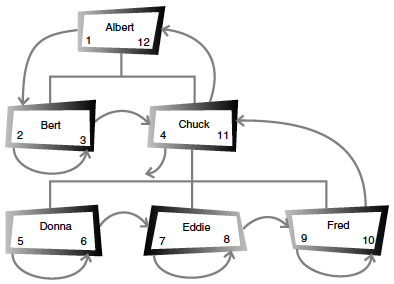
\includegraphics[scale=0.70]{imgs/NestedSetModelTree.png}
	\caption[A Nested Set Model Tree Hiererchy]{A Nested Set Model Tree Hiererchy \citep[page 46]{Celko2004}}
	\label{fig:NestedSetModelTree}
\end{figure}

Nested set model helps us on finding a node's children faster than a usual adjacency set model, where each node only keeps information about its parent node, which is the ID \citep[pages 45--47]{Celko2004}. For example, in order to find all the nodes of the root node named "Albert" in figure \ref{fig:NestedSetModelTree}, we just need to find all nodes whose left value is greater than 1, and right value is less than 12. In the adjacency list, however, we first need to find all the nodes whose parent IDs are equal to "Albert's", then for those nodes' IDs, we need to find other nodes whose parent IDs are equal to them, and it continues on until all nodes are finished in the tree in the same way.
\vspace{1cm}

The template data model in \ref{fig:UML_Prototype} keeps those left and right number information in one column named "ancestry", which is populated by a gem named Ancestry\footnote{https://github.com/stefankroes/ancestry}.

\paragraph{\ac{KVP}s Relation with a Campaign and a Message} \mbox{}\\
As shown in figure \ref{fig:UML_Prototype}, each email message can have more than one value corresponding to a key of \ac{KVP}. This allows us to identify when a \ac{KVP} is added to a message that belongs to a respondent. Keys are organized according to campaigns; therefore, same key's value can be used in different campaigns for different purposes. This is mainly because a word chosen as a key can have different meanings, depending on context.
\vspace{1cm}

After getting an overview of the technical implementation of the prototype, the next section will focus on the evaluation of the prototype by pointing out the missing features of initial requirements due to the limitations on the existing email client, and what new ideas were emerged after the informal user test within the Stanford University.

\section{Evaluation of the Prototype}
\label{sec:4.3:EvalProt}

In this section, we will analyze the limitations of the prototype, despite the fact that it was able to fulfill most of the requirements mentioned in section \ref{subsec:4.2.1:ProtReqiAnal}. Some of these limitations are related with the development of a prototype from an existing application, whose main purpose is different than that of a regular email client. One of the reasons for making a prototype is to let developers and users conceptualize different requirements or review the existing ones. In here is where we will also mention new and different requirements we deducted as we went through the whole process, as well as after the informal user test within the Stanford \ac{HCI} group and with an organization at Stanford University conducting mass email communication regularly to reach their community. As an informal user test, we asked the participants to use the prototype instead of their regular applications or methods to conduct a mass email communication, and collected the feedback.

\subsection{Limitation of the Existing Application}
\label{subsec:4.3.1:LimiEmaiVale}

As mentioned, using EmailValet as an email client on developing a prototype helped us to save time and effort. However, there were some limitations present with it since it focuses on crowd-assisted task manager actions, rather than a simple email client.

\paragraph{Number of Message Limitation}
One of the problems encountered with EmailValet was the limit on the amount of messages synchronized from Gmail. It is limited to the latest 100 messages, to maintain EmailValet's privacy and accountability \citep{Kokkalis2013}. However, a mass email campaign will quickly reach that given limit, which may ignore older emails.

\paragraph{Different Inbox Purpose}
EmailValet offers an email client with a task manager feature, as a replacement to everyone's regular email client. However, a mass email communication is not something a person needs to resort as frequent as a personal email communication. Therefore, a mass email communication application should be separated from a person's regular inbox, since it does not need to show all their emails, except those related to an email campaign. Combining both inboxes also resulted to some drawbacks on the performance while it was synchronizing with Gmail to fetch new emails. It is because EmailValet was also performing some additional steps during the synchronization on the side, such as checking and comparing message headers for changes in the earlier messages up to a date.

\subsection{Limitation of the Prototype}
\label{subsec:4.3.2:ProtDesi}

\paragraph{\ac{KVP}s Relation} In the prototype design, each value of a key belongs to an email message of a respondent. However, we need to see that all \ac{KVP}s are aggregated in a certain way when we browse a set of messages belonging to a specific person. Therefore, assigning \ac{KVP}s to an email message actually means assigning them to a recipient in a mass email campaign. This requires keeping each individual recipient in a separate data model, and relating it with the existing EmailValet's design. Since we have already identified the limitations of EmailValet in the previous section, the decision was to add those enhancements into a new application.

\paragraph{Getting Contact List into the System}
During the informal user test at the Stanford \ac{HCI} group, we realized that the people who performs such mass email communication import their recipient list from a spreadsheet, or a similar data file. Since, the prototype requires them to input a recipient list in a special syntax as mentioned in section \ref{subsec:4.2.2:ProtSyst}, this requires the users to change their existing contact list in a format that the prototype will be able to parse with. This reduces flexibility and adds additional effort on the researchers, whose contact list is already in a data file. With this said, it is a feature considered to be implemented on a different project, separate from EmailValet. 

\section{Conclusion}
\label{sec:4.4:Conc}
In this section, a mass email communication concept was introduced with an illustrative scenario. We pointed out how it could be possible to reduce the efforts on the researchers' side while increasing the personalization of the emails at the same time. Later on, we converted those ideas into software requirements for the prospective prototype, where we introduced its features and architecture. Finally, the informal user test helped us to evaluate the prototype to find out its limitations and to emerge new requirements, which made the basis to the next chapter, where the mentioned limitations are removed and the new requirements are reflected during the final application's iterative design cycles.

\clearemptydoublepage

\begin{comment}
--> message id yi nasil kullanigini yaz
- fotolar daki guzel database diagramlari kullan

--> FOOTNOTE: ORM niye table demiyon da data model diyon acikla

 Some of those information are related with message threading, where email clients recognized of a message is a reply to another message

- goes into details, so you won't need to talk about in the final product
- Sync process

--> Sonra chapter da IMAP e de deyin biraz buna bakarak gdoc: Myriad - Developer Documentation [Fetching]
--> bu prototype aklimiza gelen ilk ozelligi de anlatiyor de
--> bi section da sorunlar neydi diye yaz bunla ilgili
--> Google Formla nasil kolay data aliniyor diye bahset
--> KVP ler sadece son kampnyayala ilgili, hepsi olsa daha iyi olurdu: drawbacks of prototype'a yaz bunu

difficulty to pick a proper one , --> also no need to see old templates aga in since conversation got advanced


--> kimse boyle bir view sunmuyodu yaz, zendesk de var ama sadece bir kisi icin. Diger ozellikleri de saglayan app yok piyasa da diye ekleme yap

--> don't write a generic email, but personalized, effort var

--> there are many cases for maybe case
--> burada visulization koy ver graph i yapistir. listing olsun dashlerler tree yap
--> yukardakileri paragrah title'i kullnarka yaz

only supports hi part, not all

--> Improvements on the content


--> simdi neler olsa kolaytiririza basla

--> write something about this as well: http://blog.mailchimp.com/how-gmails-new-inbox-is-affecting-open-rates/
-->Merge tags allow you to dynamically add content to your email. 

--> Constant Contact'a limitation lari ekle \cite{ConstantContactInc.2011}, same for \cite{TheRocketScienceGroupLLC2013e}

Exploration
Have they taken any online courses before?

--> - Don�t forget Michael�s graph about golden standard
--> flow chart like in slides
--> - Asking follow-up questions are limited in other methods (see the book page 22: Beyond The Usability Lab - Conducting Large Scale Online User Experience Studies(2010))

\end{comment}